% Options for packages loaded elsewhere
\PassOptionsToPackage{unicode}{hyperref}
\PassOptionsToPackage{hyphens}{url}
\PassOptionsToPackage{dvipsnames,svgnames,x11names}{xcolor}
%
\documentclass[
  a4paper,
  DIV=11]{scrreprt}

\usepackage{amsmath,amssymb}
\usepackage{lmodern}
\usepackage{iftex}
\ifPDFTeX
  \usepackage[T1]{fontenc}
  \usepackage[utf8]{inputenc}
  \usepackage{textcomp} % provide euro and other symbols
\else % if luatex or xetex
  \usepackage{unicode-math}
  \defaultfontfeatures{Scale=MatchLowercase}
  \defaultfontfeatures[\rmfamily]{Ligatures=TeX,Scale=1}
\fi
% Use upquote if available, for straight quotes in verbatim environments
\IfFileExists{upquote.sty}{\usepackage{upquote}}{}
\IfFileExists{microtype.sty}{% use microtype if available
  \usepackage[]{microtype}
  \UseMicrotypeSet[protrusion]{basicmath} % disable protrusion for tt fonts
}{}
\makeatletter
\@ifundefined{KOMAClassName}{% if non-KOMA class
  \IfFileExists{parskip.sty}{%
    \usepackage{parskip}
  }{% else
    \setlength{\parindent}{0pt}
    \setlength{\parskip}{6pt plus 2pt minus 1pt}}
}{% if KOMA class
  \KOMAoptions{parskip=half}}
\makeatother
\usepackage{xcolor}
\usepackage[normalem]{ulem}
\setlength{\emergencystretch}{3em} % prevent overfull lines
\setcounter{secnumdepth}{5}
% Make \paragraph and \subparagraph free-standing
\ifx\paragraph\undefined\else
  \let\oldparagraph\paragraph
  \renewcommand{\paragraph}[1]{\oldparagraph{#1}\mbox{}}
\fi
\ifx\subparagraph\undefined\else
  \let\oldsubparagraph\subparagraph
  \renewcommand{\subparagraph}[1]{\oldsubparagraph{#1}\mbox{}}
\fi

\usepackage{color}
\usepackage{fancyvrb}
\newcommand{\VerbBar}{|}
\newcommand{\VERB}{\Verb[commandchars=\\\{\}]}
\DefineVerbatimEnvironment{Highlighting}{Verbatim}{commandchars=\\\{\}}
% Add ',fontsize=\small' for more characters per line
\usepackage{framed}
\definecolor{shadecolor}{RGB}{241,243,245}
\newenvironment{Shaded}{\begin{snugshade}}{\end{snugshade}}
\newcommand{\AlertTok}[1]{\textcolor[rgb]{0.68,0.00,0.00}{#1}}
\newcommand{\AnnotationTok}[1]{\textcolor[rgb]{0.37,0.37,0.37}{#1}}
\newcommand{\AttributeTok}[1]{\textcolor[rgb]{0.40,0.45,0.13}{#1}}
\newcommand{\BaseNTok}[1]{\textcolor[rgb]{0.68,0.00,0.00}{#1}}
\newcommand{\BuiltInTok}[1]{\textcolor[rgb]{0.00,0.23,0.31}{#1}}
\newcommand{\CharTok}[1]{\textcolor[rgb]{0.13,0.47,0.30}{#1}}
\newcommand{\CommentTok}[1]{\textcolor[rgb]{0.37,0.37,0.37}{#1}}
\newcommand{\CommentVarTok}[1]{\textcolor[rgb]{0.37,0.37,0.37}{\textit{#1}}}
\newcommand{\ConstantTok}[1]{\textcolor[rgb]{0.56,0.35,0.01}{#1}}
\newcommand{\ControlFlowTok}[1]{\textcolor[rgb]{0.00,0.23,0.31}{#1}}
\newcommand{\DataTypeTok}[1]{\textcolor[rgb]{0.68,0.00,0.00}{#1}}
\newcommand{\DecValTok}[1]{\textcolor[rgb]{0.68,0.00,0.00}{#1}}
\newcommand{\DocumentationTok}[1]{\textcolor[rgb]{0.37,0.37,0.37}{\textit{#1}}}
\newcommand{\ErrorTok}[1]{\textcolor[rgb]{0.68,0.00,0.00}{#1}}
\newcommand{\ExtensionTok}[1]{\textcolor[rgb]{0.00,0.23,0.31}{#1}}
\newcommand{\FloatTok}[1]{\textcolor[rgb]{0.68,0.00,0.00}{#1}}
\newcommand{\FunctionTok}[1]{\textcolor[rgb]{0.28,0.35,0.67}{#1}}
\newcommand{\ImportTok}[1]{\textcolor[rgb]{0.00,0.46,0.62}{#1}}
\newcommand{\InformationTok}[1]{\textcolor[rgb]{0.37,0.37,0.37}{#1}}
\newcommand{\KeywordTok}[1]{\textcolor[rgb]{0.00,0.23,0.31}{#1}}
\newcommand{\NormalTok}[1]{\textcolor[rgb]{0.00,0.23,0.31}{#1}}
\newcommand{\OperatorTok}[1]{\textcolor[rgb]{0.37,0.37,0.37}{#1}}
\newcommand{\OtherTok}[1]{\textcolor[rgb]{0.00,0.23,0.31}{#1}}
\newcommand{\PreprocessorTok}[1]{\textcolor[rgb]{0.68,0.00,0.00}{#1}}
\newcommand{\RegionMarkerTok}[1]{\textcolor[rgb]{0.00,0.23,0.31}{#1}}
\newcommand{\SpecialCharTok}[1]{\textcolor[rgb]{0.37,0.37,0.37}{#1}}
\newcommand{\SpecialStringTok}[1]{\textcolor[rgb]{0.13,0.47,0.30}{#1}}
\newcommand{\StringTok}[1]{\textcolor[rgb]{0.13,0.47,0.30}{#1}}
\newcommand{\VariableTok}[1]{\textcolor[rgb]{0.07,0.07,0.07}{#1}}
\newcommand{\VerbatimStringTok}[1]{\textcolor[rgb]{0.13,0.47,0.30}{#1}}
\newcommand{\WarningTok}[1]{\textcolor[rgb]{0.37,0.37,0.37}{\textit{#1}}}

\providecommand{\tightlist}{%
  \setlength{\itemsep}{0pt}\setlength{\parskip}{0pt}}\usepackage{longtable,booktabs,array}
\usepackage{calc} % for calculating minipage widths
% Correct order of tables after \paragraph or \subparagraph
\usepackage{etoolbox}
\makeatletter
\patchcmd\longtable{\par}{\if@noskipsec\mbox{}\fi\par}{}{}
\makeatother
% Allow footnotes in longtable head/foot
\IfFileExists{footnotehyper.sty}{\usepackage{footnotehyper}}{\usepackage{footnote}}
\makesavenoteenv{longtable}
\usepackage{graphicx}
\makeatletter
\def\maxwidth{\ifdim\Gin@nat@width>\linewidth\linewidth\else\Gin@nat@width\fi}
\def\maxheight{\ifdim\Gin@nat@height>\textheight\textheight\else\Gin@nat@height\fi}
\makeatother
% Scale images if necessary, so that they will not overflow the page
% margins by default, and it is still possible to overwrite the defaults
% using explicit options in \includegraphics[width, height, ...]{}
\setkeys{Gin}{width=\maxwidth,height=\maxheight,keepaspectratio}
% Set default figure placement to htbp
\makeatletter
\def\fps@figure{htbp}
\makeatother
\newlength{\cslhangindent}
\setlength{\cslhangindent}{1.5em}
\newlength{\csllabelwidth}
\setlength{\csllabelwidth}{3em}
\newlength{\cslentryspacingunit} % times entry-spacing
\setlength{\cslentryspacingunit}{\parskip}
\newenvironment{CSLReferences}[2] % #1 hanging-ident, #2 entry spacing
 {% don't indent paragraphs
  \setlength{\parindent}{0pt}
  % turn on hanging indent if param 1 is 1
  \ifodd #1
  \let\oldpar\par
  \def\par{\hangindent=\cslhangindent\oldpar}
  \fi
  % set entry spacing
  \setlength{\parskip}{#2\cslentryspacingunit}
 }%
 {}
\usepackage{calc}
\newcommand{\CSLBlock}[1]{#1\hfill\break}
\newcommand{\CSLLeftMargin}[1]{\parbox[t]{\csllabelwidth}{#1}}
\newcommand{\CSLRightInline}[1]{\parbox[t]{\linewidth - \csllabelwidth}{#1}\break}
\newcommand{\CSLIndent}[1]{\hspace{\cslhangindent}#1}

\usepackage{amsmath}
\usepackage{booktabs}
\usepackage{caption}
\usepackage{longtable}
\usepackage{array}
\usepackage{multirow}
\usepackage{wrapfig}
\usepackage{float}
\usepackage{colortbl}
\usepackage{pdflscape}
\usepackage{tabu}
\usepackage{threeparttable}
\usepackage{threeparttablex}
\usepackage[normalem]{ulem}
\usepackage{makecell}
\usepackage{xcolor}
\KOMAoption{captions}{tableheading}
\makeatletter
\@ifpackageloaded{tcolorbox}{}{\usepackage[many]{tcolorbox}}
\@ifpackageloaded{fontawesome5}{}{\usepackage{fontawesome5}}
\definecolor{quarto-callout-color}{HTML}{909090}
\definecolor{quarto-callout-note-color}{HTML}{0758E5}
\definecolor{quarto-callout-important-color}{HTML}{CC1914}
\definecolor{quarto-callout-warning-color}{HTML}{EB9113}
\definecolor{quarto-callout-tip-color}{HTML}{00A047}
\definecolor{quarto-callout-caution-color}{HTML}{FC5300}
\definecolor{quarto-callout-color-frame}{HTML}{acacac}
\definecolor{quarto-callout-note-color-frame}{HTML}{4582ec}
\definecolor{quarto-callout-important-color-frame}{HTML}{d9534f}
\definecolor{quarto-callout-warning-color-frame}{HTML}{f0ad4e}
\definecolor{quarto-callout-tip-color-frame}{HTML}{02b875}
\definecolor{quarto-callout-caution-color-frame}{HTML}{fd7e14}
\makeatother
\makeatletter
\makeatother
\makeatletter
\@ifpackageloaded{bookmark}{}{\usepackage{bookmark}}
\makeatother
\makeatletter
\@ifpackageloaded{caption}{}{\usepackage{caption}}
\AtBeginDocument{%
\ifdefined\contentsname
  \renewcommand*\contentsname{Inhaltsverzeichnis}
\else
  \newcommand\contentsname{Inhaltsverzeichnis}
\fi
\ifdefined\listfigurename
  \renewcommand*\listfigurename{Abbildungsverzeichnis}
\else
  \newcommand\listfigurename{Abbildungsverzeichnis}
\fi
\ifdefined\listtablename
  \renewcommand*\listtablename{Tabellenverzeichnis}
\else
  \newcommand\listtablename{Tabellenverzeichnis}
\fi
\ifdefined\figurename
  \renewcommand*\figurename{Abbildung}
\else
  \newcommand\figurename{Abbildung}
\fi
\ifdefined\tablename
  \renewcommand*\tablename{Tabelle}
\else
  \newcommand\tablename{Tabelle}
\fi
}
\@ifpackageloaded{float}{}{\usepackage{float}}
\floatstyle{ruled}
\@ifundefined{c@chapter}{\newfloat{codelisting}{h}{lop}}{\newfloat{codelisting}{h}{lop}[chapter]}
\floatname{codelisting}{Listing}
\newcommand*\listoflistings{\listof{codelisting}{Listingverzeichnis}}
\usepackage{amsthm}
\theoremstyle{definition}
\newtheorem{example}{Beispiel}[chapter]
\theoremstyle{remark}
\renewcommand*{\proofname}{Beweis}
\newtheorem*{remark}{Anmerkung}
\newtheorem*{solution}{Lösung}
\makeatother
\makeatletter
\@ifpackageloaded{caption}{}{\usepackage{caption}}
\@ifpackageloaded{subcaption}{}{\usepackage{subcaption}}
\makeatother
\makeatletter
\@ifpackageloaded{tcolorbox}{}{\usepackage[many]{tcolorbox}}
\makeatother
\makeatletter
\@ifundefined{shadecolor}{\definecolor{shadecolor}{rgb}{.97, .97, .97}}
\makeatother
\makeatletter
\makeatother
\ifLuaTeX
\usepackage[bidi=basic]{babel}
\else
\usepackage[bidi=default]{babel}
\fi
\babelprovide[main,import]{ngerman}
% get rid of language-specific shorthands (see #6817):
\let\LanguageShortHands\languageshorthands
\def\languageshorthands#1{}
\ifLuaTeX
  \usepackage{selnolig}  % disable illegal ligatures
\fi
\IfFileExists{bookmark.sty}{\usepackage{bookmark}}{\usepackage{hyperref}}
\IfFileExists{xurl.sty}{\usepackage{xurl}}{} % add URL line breaks if available
\urlstyle{same} % disable monospaced font for URLs
\hypersetup{
  pdftitle={Start:Bayes!},
  pdfauthor={Sebastian Sauer},
  pdflang={de},
  colorlinks=true,
  linkcolor={blue},
  filecolor={Maroon},
  citecolor={Blue},
  urlcolor={Blue},
  pdfcreator={LaTeX via pandoc}}

\title{Start:Bayes!}
\author{Sebastian Sauer}
\date{11.01.23}

\begin{document}
\maketitle
\ifdefined\Shaded\renewenvironment{Shaded}{\begin{tcolorbox}[interior hidden, enhanced, boxrule=0pt, breakable, frame hidden, sharp corners, borderline west={3pt}{0pt}{shadecolor}]}{\end{tcolorbox}}\fi

\renewcommand*\contentsname{Inhaltsverzeichnis}
{
\hypersetup{linkcolor=}
\setcounter{tocdepth}{2}
\tableofcontents
}
\bookmarksetup{startatroot}

\hypertarget{hinweise}{%
\chapter*{Hinweise}\label{hinweise}}
\addcontentsline{toc}{chapter}{Hinweise}

\markboth{Hinweise}{Hinweise}

\begin{figure}

{\centering 
\includegraphics[width=0.5\textwidth,height=\textheight]{./img/Golem_hex.png}

}

\caption{Bayes:Start! Bildquelle: Klara Schaumann}

\end{figure}

\hypertarget{lernziele}{%
\section*{Lernziele}\label{lernziele}}
\addcontentsline{toc}{section}{Lernziele}

\markright{Lernziele}

Nach diesem Kurs sollten Sie \ldots{}

\begin{itemize}
\tightlist
\item
  grundlegende Konzepte der Inferenzstatistik mit Bayes verstehen und
  mit R anwenden können
\item
  gängige einschlägige Forschungsfragen in statistische Modelle
  übersetzen und mit R auswerten können
\item
  kausale Forschungsfragen in statistische Modelle übersetzen und prüfen
  können
\item
  die Güte und Grenze von statistischen Modellen einschätzen können
\end{itemize}

\hypertarget{voraussetzungen}{%
\section*{Voraussetzungen}\label{voraussetzungen}}
\addcontentsline{toc}{section}{Voraussetzungen}

\markright{Voraussetzungen}

Um von diesem Kurs am besten zu profitieren, sollten Sie folgendes
Wissen mitbringen:

\begin{itemize}
\tightlist
\item
  grundlegende Kenntnisse im Umgang mit R, möglichst auch mit dem
  tidyverse
\item
  grundlegende Kenntnisse der deskriptiven Statistik
\item
  grundlegende Kenntnis der Regressionsanalyse
\end{itemize}

\hypertarget{software}{%
\section*{Software}\label{software}}
\addcontentsline{toc}{section}{Software}

\markright{Software}

Installieren Sie
\href{https://data-se.netlify.app/2021/11/30/installation-von-r-und-seiner-freunde/}{R
und seine Freunde}. Für die Bayes-Inferenz brauchen Sie\footnote{nicht
  gleich zu Beginn, aber nach 2-3 Wochen} zusätzliche Software, was
leider etwas Zusatzaufwand erfordert. Lesen Sie
\href{https://data-se.netlify.app/2022/01/28/bayes-software-installieren-f\%C3\%BCr-r/}{hier}
die Hinweise dazu. Installieren Sie die folgende R-Pakete\footnote{falls
  Sie die Pakete schon installiert haben, könnten Sie mal in RStudio auf
  ``update.packages'' klicken}:

\begin{itemize}
\tightlist
\item
  tidyverse
\item
  rstanarm
\item
  easystats
\item
  weitere Pakete werden im Unterricht bekannt gegeben (es schadet aber
  nichts, jetzt schon Pakete nach eigenem Ermessen zu installieren)
\end{itemize}

\href{https://github.com/sebastiansauer/Lehre}{R Syntax aus dem
Unterricht} findet sich im Github-Repo bzw. Ordner zum jeweiligen
Semester.

\hypertarget{pdf-version}{%
\section*{PDF-Version}\label{pdf-version}}
\addcontentsline{toc}{section}{PDF-Version}

\markright{PDF-Version}

-- EXPERIMENTAL 🔬🧪 -- EXPERIMENTAL

Von diesem ``Webbuch'' (HTML-Format) gibt es
\href{Start-Bayes!.pdf}{hier eine PDF-Version}. Die PDF-Version eignet
sich zum Ausdrucken und zur Offline-Nutzung.

Allerdings wurden die Inhalte \emph{in erster Linie für ein
Webbuch-Format} formatiert, die PDF-Ausgabe ist daher nicht ideal. Es
ist empfehlenswert, mit der Webbuch-Version zu arbeiten. Außerdem wird
die PDF-Version nicht ganz aktuell gehalten - die aktuelle Version ist
immer die Webbuch-Variante. Prüfen Sie im Zweifel das Datum der
Erstellung des Dokuments.

\hypertarget{lernhilfen}{%
\section*{Lernhilfen}\label{lernhilfen}}
\addcontentsline{toc}{section}{Lernhilfen}

\markright{Lernhilfen}

\hypertarget{videos}{%
\subsection*{Videos}\label{videos}}
\addcontentsline{toc}{subsection}{Videos}

Auf dem
\href{https://www.youtube.com/channel/UCkvdtj8maE7g-SOCh4aDB9g}{YouTube-Kanal
des Autors} finden sich eine Reihe von Videos mit Bezug zum Inhalt
dieses Buchs. Besonders
\href{https://www.youtube.com/playlist?list=PLRR4REmBgpIGVptiSN-qDVEJKfFnUqDyL}{diese
Playlist} passt zu den Inhalten dieses Buchs.

\hypertarget{online-zusammenarbeit}{%
\subsection*{Online-Zusammenarbeit}\label{online-zusammenarbeit}}
\addcontentsline{toc}{subsection}{Online-Zusammenarbeit}

Hier finden Sie einige Werkzeuge, die das Online-Zusammenarbeiten
vereinfachen:

\begin{itemize}
\tightlist
\item
  \href{https://frag.jetzt/home}{Frag-Jetzt-Raum zum anonymen Fragen
  stellen während des Unterrichts}. Der Keycode wird Ihnen bei Bedarf
  vom Dozenten bereitgestellt.
\item
  \href{https://de.padlet.com/}{Padlet} zum einfachen (und anonymen)
  Hochladen von Arbeitsergebnissen der Studentis im Unterricht. Wir
  nutzen es als eine Art Pinwand zum Sammeln von Arbeitsbeiträgen. Die
  Zugangsdaten stellt Ihnen der Dozent bereit.
\end{itemize}

\hypertarget{modulzeitplan}{%
\section*{Modulzeitplan}\label{modulzeitplan}}
\addcontentsline{toc}{section}{Modulzeitplan}

\markright{Modulzeitplan}

\begin{longtable}{rlll}
\toprule
Nr & Thema & Datum & Kommentar \\ 
\midrule
1 & Was ist Inferenz? & 3. - 7. Okt. 2022 & Erster Termin: 4. Okt. 22, 14.15-15.00 \\ 
2 & Wahrscheinlichkeit & 10. - 14. Okt. 22 & NA \\ 
3 & Verteilungen & 17. - 21. Okt. 22 & NA \\ 
4 & Globusversuch & 24. - 28. Okt. 22 & NA \\ 
5 & Aufhol-Woche & 31. Okt. - 4. Nov. 22 & Am Di., 1.11. entfällt die Vorlesung. Am Do., 3. 11. entfällt die Übung. \\ 
6 & Frag die Post & 7. - 11. Nov. 22 & Ab diese Woche benötigen wir rstanarm. \\ 
NA & NA & 14. - 18. Nov. 22 & Blockwoche: Kein regulärer Unterricht \\ 
7 & Gauss-Modelle & 21. - 25. Nov. 22 & NA \\ 
8 & Lineare Modelle & 28. Nov. - 2. Dez. 22 & NA \\ 
9 & Metrische AV & 5. Dez. - 9. Dez. 22 & NA \\ 
10 & Kausalinferenz 1 & 12. - 16. Dez. 22 & NA \\ 
11 & Kausalinferenz 2 & 19. - 23. Dez. 22 & NA \\ 
NA & NA & NA & Jahreswechsel: Kein Unterricht \\ 
12 & Abschluss & 9. Jan. 23 - 13. Jan. 23 & NA \\ 
\bottomrule
\end{longtable}

\hypertarget{literatur}{%
\section*{Literatur}\label{literatur}}
\addcontentsline{toc}{section}{Literatur}

\markright{Literatur}

Pro Thema wird Literatur ausgewiesen.

\hypertarget{technische-details}{%
\section*{Technische Details}\label{technische-details}}
\addcontentsline{toc}{section}{Technische Details}

\markright{Technische Details}

Dieses Dokument wurde erzeugt am/um 2023-01-06 11:07:30.

\begin{verbatim}
## - Session info ---------------------------------------------------------------
##  setting  value
##  version  R version 4.2.1 (2022-06-23)
##  os       macOS Big Sur ... 10.16
##  system   x86_64, darwin17.0
##  ui       X11
##  language (EN)
##  collate  en_US.UTF-8
##  ctype    en_US.UTF-8
##  tz       Europe/Berlin
##  date     2023-01-06
##  pandoc   2.19.2 @ /Applications/RStudio.app/Contents/Resources/app/quarto/bin/tools/ (via rmarkdown)
## 
## - Packages -------------------------------------------------------------------
##  package     * version date (UTC) lib source
##  assertthat    0.2.1   2019-03-21 [1] CRAN (R 4.2.0)
##  cellranger    1.1.0   2016-07-27 [1] CRAN (R 4.2.0)
##  cli           3.5.0   2022-12-20 [1] CRAN (R 4.2.0)
##  colorout    * 1.2-2   2022-06-13 [1] local
##  colorspace    2.0-3   2022-02-21 [1] CRAN (R 4.2.0)
##  DBI           1.1.3   2022-06-18 [1] CRAN (R 4.2.0)
##  digest        0.6.31  2022-12-11 [1] CRAN (R 4.2.0)
##  dplyr         1.0.10  2022-09-01 [1] CRAN (R 4.2.0)
##  evaluate      0.19    2022-12-13 [1] CRAN (R 4.2.0)
##  fansi         1.0.3   2022-03-24 [1] CRAN (R 4.2.0)
##  fastmap       1.1.0   2021-01-25 [1] CRAN (R 4.2.0)
##  generics      0.1.3   2022-07-05 [1] CRAN (R 4.2.0)
##  ggplot2       3.4.0   2022-11-04 [1] CRAN (R 4.2.0)
##  glue          1.6.2   2022-02-24 [1] CRAN (R 4.2.0)
##  gt            0.8.0   2022-11-16 [1] CRAN (R 4.2.0)
##  gtable        0.3.1   2022-09-01 [1] CRAN (R 4.2.0)
##  htmltools     0.5.4   2022-12-07 [1] CRAN (R 4.2.0)
##  jsonlite      1.8.4   2022-12-06 [1] CRAN (R 4.2.0)
##  knitr         1.41    2022-11-18 [1] CRAN (R 4.2.0)
##  lifecycle     1.0.3   2022-10-07 [1] CRAN (R 4.2.0)
##  magrittr      2.0.3   2022-03-30 [1] CRAN (R 4.2.0)
##  munsell       0.5.0   2018-06-12 [1] CRAN (R 4.2.0)
##  pillar        1.8.1   2022-08-19 [1] CRAN (R 4.2.0)
##  pkgconfig     2.0.3   2019-09-22 [1] CRAN (R 4.2.0)
##  R6            2.5.1   2021-08-19 [1] CRAN (R 4.2.0)
##  readxl        1.4.1   2022-08-17 [1] CRAN (R 4.2.0)
##  rlang         1.0.6   2022-09-24 [1] CRAN (R 4.2.0)
##  rmarkdown     2.19    2022-12-15 [1] CRAN (R 4.2.0)
##  rstudioapi    0.14    2022-08-22 [1] CRAN (R 4.2.0)
##  scales        1.2.1   2022-08-20 [1] CRAN (R 4.2.0)
##  sessioninfo   1.2.2   2021-12-06 [1] CRAN (R 4.2.0)
##  stringi       1.7.8   2022-07-11 [1] CRAN (R 4.2.0)
##  stringr       1.5.0   2022-12-02 [1] CRAN (R 4.2.0)
##  tibble        3.1.8   2022-07-22 [1] CRAN (R 4.2.0)
##  tidyselect    1.2.0   2022-10-10 [1] CRAN (R 4.2.0)
##  utf8          1.2.2   2021-07-24 [1] CRAN (R 4.2.0)
##  vctrs         0.5.1   2022-11-16 [1] CRAN (R 4.2.0)
##  withr         2.5.0   2022-03-03 [1] CRAN (R 4.2.0)
##  xfun          0.36    2022-12-21 [1] CRAN (R 4.2.0)
##  yaml          2.3.6   2022-10-18 [1] CRAN (R 4.2.0)
## 
##  [1] /Users/sebastiansaueruser/Rlibs
##  [2] /Library/Frameworks/R.framework/Versions/4.2/Resources/library
## 
## ------------------------------------------------------------------------------
\end{verbatim}

\bookmarksetup{startatroot}

\hypertarget{pruxfcfung}{%
\chapter{Prüfung}\label{pruxfcfung}}

\hypertarget{pruxfcfungleistung}{%
\section{Prüfungleistung}\label{pruxfcfungleistung}}

Die Prüfungsleistung besteht aus einer \emph{Open-Book-Prüfung}.

\hypertarget{grundsuxe4tzliches}{%
\section{Grundsätzliches}\label{grundsuxe4tzliches}}

Die folgenden Hinweise gelten \emph{grundsätzlich}, d.h. \emph{soweit
nicht anders} in der jeweiligen Prüfung bzw. der jeweiligen Aufgabe
angegeben.

Nichtbeachten von Prüfungshinweisen kann zu Punkteabzug oder
Nichtbestehen führen.

\hypertarget{wiederholungspruxfcfungen}{%
\section{Wiederholungsprüfungen}\label{wiederholungspruxfcfungen}}

\begin{itemize}
\tightlist
\item
  Wenn Sie bei einer Prüfung durchgefallen sein sollten, so haben Sie
  grundsätzlich die Möglichkeit, die \emph{Prüfung zu wiederholen}.
\item
  Denken Sie daran, sich \emph{rechtzeitig} für Prüfungsleistungen
  \emph{anzumelden}; beachten Sie die Fristen.
\item
  Die Termine für die Wiederholungsprüfungen werden stets
  zusammen/zeitgleich mit denen der regulären Prüfungen bekannt gegeben.
\item
  Wird ein Modul im laufenden Semester nicht angeboten, gibt es eine
  Wiederholungsprüfung.
\item
  Relevanter Stoff und formale Bedingungen (wie Prüfungsform) sind
  \emph{grundsätzlich identisch zur letzten abgehaltenen Prüfung des
  Moduls} (d.h. sofern nicht anders angegeben). Daher sind
  Wiederholungsprüfungen vom Anspruch vergleichbar wie die reguläre
  Klausur. Die Prüfungen sollen möglichst gleich vom Anspruch sein, um
  Fairness zu gewährleisten.
\item
  Beachten Sie immer die \emph{Hinweise}, die für die
  Wiederholungsprüfung angegeben sind. Im Einzelfall keine eine
  Wiederholungsprüfung von der vorherigen Prüfung stärker abweichen. Es
  gelten immer die Regeln, die dis Dozenti bei der jeweiligen
  Wiederholungsprüfung veröffentlicht hat.
\item
  Wird ein \emph{Modul im laufenden Semester} angeboten, so gibt es
  keine Wiederholungsprüfung. Stattdessen können Sie ggf. an der
  regulären Klausur des Moduls teilnehmen. Es gilt der aktuelle Stoff
  bzw. die aktuellen formalen Bedingungen. Es ist möglich, dass der
  Stoff sich dann substanziell ändert; meist halten sich die Änderungen
  (im Stoff) aber in Rahmen.
\item
  Sprechen Sie die \emph{Moduldozentis an für Details zur Prüfung} (bzw.
  lesen Sie vorab auf jeweiligen Modulseite in Moodle nach).
\item
  Manchmal fragen Studentis nach einer \emph{Empfehlung}, ob es besser
  ist, eine Prüfung zu verschieben, wenn man sich nicht ausreichend
  vorbereiten konnte. Es ist schwer, eine Empfehlung pauschal abzugeben,
  es kommt auf den Einzelfall an. Grundsätzlich rate ich aber dazu,
  Prüfungen nicht zu verschieben: Schließlich könnte in einem folgenden
  Semester wieder ein unvorhergesehenes Problem auftreten.
\item
  Bei Fragen zum \emph{Prüfungsrecht} sprechen Sie bitte die
  \emph{Studienberatung} an.
\end{itemize}

\hypertarget{pruxfcfungsstoff}{%
\section{Prüfungsstoff}\label{pruxfcfungsstoff}}

Prüfungsrelevanter Stoff ist alles, was im Unterricht behandelt wurde,
sofern es nicht explizit (und schriftlich) als ``nicht
prüfungsrelevant'' gekennzeichnet ist.

\hypertarget{bearbeitungshinweise}{%
\section{Bearbeitungshinweise}\label{bearbeitungshinweise}}

\hypertarget{allgemeine-hinweise}{%
\subsection{Allgemeine Hinweise}\label{allgemeine-hinweise}}

\begin{itemize}
\tightlist
\item
  Verwenden Sie \emph{Standardwerte} (defaults) der R-Funktionen, soweit
  nicht anders in der jeweiligen Aufgabe verlangt.
\item
  Findet sich in einer Auswahlliste möglicher Antworten nicht die exakte
  Lösung, wählen Sie die \emph{am besten passende}.
\item
  \emph{Treffen Sie Annahmen}, (nur) wo nötig.
\item
  Die Prüfung besteht auch aus \emph{Single- bzw. Multiple-Choice}-
  (MC)-Aufgaben mit mehreren Antwortoptionen.
\item
  Bei Multiple-Choice-Aufgaben (MC-Aufgaben) ist zumeist genau
  \emph{eine} Antwortoption auszuwählen aus vier oder fünf
  Antwortoptionen.
\item
  Im Zweifel ist eine Aussage auf den Stoff, so wie im \emph{Unterricht}
  behandelt, zu beziehen.
\item
  Bei Fragen zu R-Syntax spielen Aspekte wie Enter-Taste o.Ä. bei der
  Beantwortung der Frage keine Rolle; diese Aspekte dürfen zu
  ignorieren.
\item
  Jede Aussage einer MC-Aufgabe ist entweder richtig oder falsch (aber
  nicht beides oder keines).
\item
  Die MC-Aufgaben sind \emph{nur mit Kreuzen} zu beantworten; Text wird
  bei der Korrektur nicht berücksichtigt.
\item
  Jede Aussage gilt \emph{ceteris paribus} (unter sonst gleichen
  Umständen). Aussagen der Art „A ist B`` (z.B. ``Menschen sind
  sterblich'') sind \emph{nur} dann als richtig auszuwählen, wenn die
  Aussage \emph{immer} richtig ist.
\item
  Falls Sie bei einer Aufgabe mehrere Antworten finden, aber nur nach
  einer gefragt ist, geben Sie nur eine an.
\item
  Falls mehrere (widersprüchliche) Antworten gegeben wurden, wird im
  Zweifel die \emph{erst genannte} gewertet.
\item
  Die Aufgabenstellung in einer Moodle-Prüfung wird erst sichtbar, wenn
  Sie den \emph{Prüfungsbedingungen} zugestimmt haben und die
  Prüfungszeit begonnen hat.
\end{itemize}

\hypertarget{aufgaben-zur-datenanalyse}{%
\subsection{Aufgaben zur Datenanalyse}\label{aufgaben-zur-datenanalyse}}

\begin{itemize}
\tightlist
\item
  Je nach Spracheinstellung in Moodle kann es sein, dass Sie als
  \emph{Dezimaltrennzeichen} ein Komma oder einen Punkt verwenden
  müssen. Moodle weist Sie, wenn Sie die Aufgabe verlassen, darauf hin,
  falls eine Zahl nicht als Zahl erkannt wurde.
\item
  \emph{Runden} Sie bei Fragen, die auf Anteile abzielen auf \emph{zwei}
  Dezimalstellen, ansonsten auf eine.
\item
  Geben Sie keine Prozentzahlen an, sondern \emph{Anteile} (also nicht
  ``50\%'', sondern ``0.5'' bzw. ``0,5'').
\item
  Bei Aufgaben, die eine Zahl als Antwort verlangen, ist \emph{nur eine
  Zahl anzugeben} (nicht etwa Buchstaben).
\item
  Alle Berechnungen, die \emph{Zufallszahlen} beinhalten, sollen mit
  \emph{fixierten Startwert} der Zufallszahlen durchgeführt werden. Es
  ist die Zahl \texttt{42} zu verwenden.
\item
  Wie auch bei den übrigen Hinweisen gelten diese Maßgaben nur soweit in
  der Prüfung nicht \emph{explizit andere Hinweise} gegeben wurden.
\item
  Wenn \emph{Stichproben simuliert} werden sollen, ziehen Sie \(10^3\)
  Zufallsstichproben.
\item
  In einigen Aufgaben kann verlangt sein, dass Sie einen
  \emph{bestimmten Datensatz in R importieren} sollen. In diesem Fall
  wird vorausgesetzt, dass Ihnen
  \href{https://vincentarelbundock.github.io/Rdatasets/articles/data.html}{diese
  Bezugsquelle} von Datensätzen bekannt ist und dass Sie wissen, wie man
  einen Datensatz in R importiert.
\item
  Achten Sie darauf, R und R-Pakete sowie R-Studio \emph{in aktueller
  Version} zu verwenden. Das Verwenden älterer Versionen kann (in
  seltenen Fällen) zu abweichenden Lösungen führen. Im Zweifel beziehen
  sich alle Aufgaben auf die jeweils aktuellste Version der verwendeten
  Software.
\item
  Wenn Sie \emph{Text eingeben} sollen: Geben Sie \emph{nur
  Kleinbuchstaben ein}. Geben Sie nur ein einziges Wort ein. Geben Sie
  keine Leerzeichen ein.
\end{itemize}

Speziell zur Bayes-Statistik:

\begin{itemize}
\tightlist
\item
  Verwenden Sie Methoden der \emph{Bayes}-Statistik für
  inferenzstatistische Analysen.
\item
  Bei Aufgaben zur ``\emph{Bayes-Box}'' (Erstellung einer
  Gitterwert-Tabelle) gelten folgende Maßgaben:

  \begin{itemize}
  \tightlist
  \item
    Handelt es sich um Parameter mit einem begrenzten Wertebereich (wie
    etwa \emph{Anteile}), so ist der ganze Wertebereich zu modellieren.
    Es sind 100 verschiedene Parameterwerte zu berechnen.
  \item
    Handelt es sich um Parameter \(X\) mit einem unbegrenzten
    Wertebereich (wie \emph{normalverteilte} Variablen), so ist der
    Wertebereich \(X-2\sigma \le X \le X+2\sigma\) zu simulieren.
  \end{itemize}
\item
  Nutzen Sie die Software \emph{Stan} in Form des R-Pakets
  \texttt{rstanarm} für Regressionsmodelle auf Basis der Bayes-Methode.
\end{itemize}

\hypertarget{teilnahmebedingungen}{%
\section{Teilnahmebedingungen}\label{teilnahmebedingungen}}

\begin{itemize}
\tightlist
\item
  Die Prüfung ist selbständig, also alleine nur durch Sie, \emph{ohne
  Hilfe Dritter}, zu absolvieren.
\item
  Die \emph{Bearbeitungszeiten} der Prüfung sind einzuhalten.
\item
  Es dürfen nur die explizit als zulässig gekennzeichneten
  \emph{Hilfsmittel} verwendet werden.
\item
  Die \emph{zulässigen} Hilfsmittel sind: Notizpapier, Stifte,
  Taschenrechner, Vorlesungsfolien, Skripte, eigene Notizen, Bücher
  sowie Quellen aus dem Internet.
\item
  Die Übernahme von Inhalten Dritter muss also solche gekennzeichnet
  (\emph{zitiert}) werden.
\item
  Eine wörtliche Übernahme (``\emph{copy-paste}'') von Inhalten Dritter
  (etwa aus einer Quelle aus dem Internet) ist unzulässig.
\item
  Bei \emph{technischen Problemen} ist sofort der Prüfer bzw. die
  Prüferin zu verständigen und das technische Problem zu dokumentieren.
  Aus der Dokumentation muss der Fehler erkenntlich sein.
\item
  Es ist \emph{untersagt}, die \emph{Prüfung} bzw. Teile daraus (z.B.
  Prüfungsfragen) zu speichern oder \emph{weiterzugeben.}
\item
  Im Übrigen gelten die allgemeinen \emph{Prüfungsregeln}.
\item
  Es darf \emph{nicht} mit anderen Personen, insbesondere nicht
  Prüflingen, \emph{kommuniziert} werden während der Prüfung. Dies gilt
  auch für den Fall von (vermeintlichen) technischen Problemen.
  Kontaktieren Sie den Prüfer, wenn Sie meinen, es liege ein technisches
  Problem vor.
\end{itemize}

\hypertarget{organisatorische-hinweise}{%
\section{Organisatorische Hinweise}\label{organisatorische-hinweise}}

\begin{itemize}
\tightlist
\item
  Etwaige weitere \emph{Stoffeingrenzungen} werden schriftlich bekannt
  gemacht (auf der Modulseite). Besondere Schwerpunkte gibt es nicht.
\item
  Soweit bestimmte Inhalte nicht explizit ausgeschlossen sind, sind alle
  Inhalte, die im Rahmen des Moduls bearbeitet wurden,
  \emph{prüfungsrelevant.}
\item
  Im Übrigen gelten die Hinweise der \emph{offiziellen Regularien} wie
  SPO, auf dem Modulsteckbrief und der APO. Bitte kontaktieren Sie die
  Studienberatung für formale oder rechtliche Fragen.
\item
  Während der Prüfung werden nur Fragen beantwortet, die für die
  Bearbeitung zwingend nötig sind (etwa bei technischen Problemen).
\item
  Es werden keine Fragen der Art ``Ist diese Aufgabe klar formuliert?''
  beantwortet während der Prüfung. Sollten Sie der Meinung sein, eine
  Frage ist unklar formuliert oder fehlerhaft, so notieren Sie dies
  bitte (z.B. im Kommentarfeld der Prüfung=. Der Prüfer untersucht im
  Nachgang die Angelegenheit. Stellt sich eine Frage als fehlerhaft oder
  unklar formuliert heraus, so wird sie von der Beurteilung
  herausgenommen.
\item
  Eine Teilnahme an der Prüfung ist nur möglich, wenn Sie den
  Teilnahmebedingungen der Prüfung zustimmen.
\item
  Die Aufgabenstellung der Prüfung wird nur während des
  Prüfungszeitraumes angezeigt.
\item
  Beachten Sie eine etwaige Gruppenteilung (zu welcher Gruppe Sie
  zugeteilt sind).
\item
  Beachten Sie die exakte Prüfungsuhrzeit (Beginn, Ende).
\item
  Prüfungszeitraum, Aufgabenstellung und sonstige Materialien können
  variieren zwischen den Prüflingen etwa aufgrund von
  Gruppeneinteilungen oder Nachteilsausgleich.
\item
  Die zusätzliche Bearbeitungszeit bei Studentis mit Nachteilsausgleich
  ist in der Aufgabenstellung bzw. der Prüfung in Moodle hinterlegt. Die
  Zeit wird automatisch um den jeweiligen Faktor erhöht.
\end{itemize}

\hypertarget{open-book-pruxfcfungen}{%
\section{Open-Book-Prüfungen}\label{open-book-pruxfcfungen}}

Einige Prüfungen werden als ``Take-home-Prüfung'' im
``Open-Book-Format'' geschrieben. Was bedeutet dies?

``Take-home-Prüfung'': Sie bearbeiten die Prüfung in Ihrem privaten
Umgebung in Moodle oder in Räumlichkeiten der Hochschule. Eine
Überwachung per Kamera findet nicht statt.

``Open-Book-Prüfung'': Sie dürfen Hilfsmittel wie Bücher und Folien
während der Prüfung nutzen.

Ihre Prüferin/Ihr Prüfer informiert Sie über das Format Ihrer Prüfung.

\hypertarget{zeitrahmen-der-pruxfcfung}{%
\section{Zeitrahmen der Prüfung}\label{zeitrahmen-der-pruxfcfung}}

Die Prüfung beginnt und endet zu einem festen Zeitpunkt. Sie sind selber
verantwortlich, die Prüfung zur korrekten Zeit zu beginnen und zu
beenden (einzureichen). Verspätete Abgaben werden u.U. als nicht
bestanden gewertet. Die Dauer der Prüfung wird Ihnen von Ihrer Prüferin
bzw. Ihrem Prüfer bekannt gegeben.

\hypertarget{technische-und-organisatorische-anforderungen-einer-open-book-pruxfcfung}{%
\section{Technische und organisatorische Anforderungen einer
Open-Book-Prüfung}\label{technische-und-organisatorische-anforderungen-einer-open-book-pruxfcfung}}

Um an einer Open-Book-Prüfung teilzunehmen, benötigen Sie IT-Ausstattung
sowie Räumlichkeiten. An IT-Ausstattung benötigen Sie einen Computer mit
Internetanschluss; ein Smartphone reicht nicht aus. Nutzen Sie Ihr
eigenes Gerät (Computer) für die Prüfung; die Hochschule stellt Ihnen
keinen Computer zur Verfügung. Sie benötigen keine Webcam und kein
Mikrofon. Ein Tablett oder Smartphone reicht nicht für die Prüfung. An
Software benötigen Sie Zugang zu Ihrem Moodle-Konto, was einen aktuellen
Internet-Browser voraussetzt. Zu den organisatorischen Anforderungen
gehören ein Raum, in dem Sie die Prüfung ungestört bearbeiten können
sowie ein Internetanschluss zum Bearbeiten der Klausur in Moodle. Bitte
benutzen Sie während der Prüfung nicht den Zurück-Button in Ihrem
Browser, wenn Sie zu einer vorherigen Frage zurückgehen wollen. Nutzen
Sie die in der Prüfung zur Verfügung gestellten Funktionen/Buttons
dafür.

\hypertarget{technische-probleme-wuxe4hrend-der-pruxfcfung}{%
\section{Technische Probleme während der
Prüfung}\label{technische-probleme-wuxe4hrend-der-pruxfcfung}}

Im Falle eines technischen Problems auf Seiten der
\emph{Prüfungsinfrastruktur} ist sofort der Prüfer zu informieren. Ein
Beispiel für so ein Problem wäre etwa der Ausfall von Moodle. Der
technische Fehler ist zu dokumentieren (z.B. Screenshot) und die
Dokumentation ist einzureichen. Bitte beachten Sie, dass der Prüfer bzw.
die Hochschule keine Gewähr übernimmt für Probleme mit Ihrer eigenen
Ausstattung.

\hypertarget{pruxfcfungsrecht}{%
\section{Prüfungsrecht}\label{pruxfcfungsrecht}}

Für die Open-Book-Prüfungg gilt die aktuelle Prüfungsordnung; die
Open-Book-Prüfung fällt \emph{nicht} unter die BayFEV.

\hypertarget{bitte-formulieren-sie-beanstandungen-nachvollziehbar}{%
\section{Bitte formulieren Sie Beanstandungen
nachvollziehbar}\label{bitte-formulieren-sie-beanstandungen-nachvollziehbar}}

Falls Sie einen Fehler in einer Aufgabenstellung finden (die der Prüfer
zu bestanden hat): Freuen Sie sich! In diesem Fall wird zu Ihren Gunsten
entschieden.

Damit ich Ihre Beanstandung prüfen kann, ist es nötig, dass ich Ihre
\emph{Beanstandung} nachprüfen kann: \emph{Zeigen} Sie mir meinen
Fehler. Es reicht \emph{nicht} zu sagen ``es hat bei mir nicht
funktioniert''. Wenn Sie etwa der Meinung sind, dass es die Variable
``year'' im Datensatz ``penguins'' nicht gebe, dann schicken Sie mir den
R-Code, der an ansprechender Stelle einen Fehler aufwirft (aber
\emph{ansonsten lauffähig} ist). Ein Screenshot kann in einigen
Situationen helfen, wenn aber nur ein Teil der Syntax zu sehen ist, ist
er nicht ausreichend: Wenn der Befehl \texttt{data(penguins)} nicht
funktioniert, so ist zu prüfen, ob Sie vorab mit
\texttt{library(palmerpenguins)} das relevante Paket gestartet haben.
Andernfalls kann \texttt{data(penguins)} nicht funktionieren und der
Fehler läge damit bei Ihnen.

\href{https://data-se.netlify.app/2022/01/31/erbie-einfache-reproduzierbare-beispiele-ihres-problems-mit-r-syntax/}{Hier}
finden Sie Hinweise für \emph{e}infache, \emph{r}eproduzierbare
\emph{Bei}spiele (ERBies); vgl. Sauer (2019), Kap. 3.8.2 (S. 33).

Die gleiche Messlatte lege ich an mich an: Ich stelle eine Musterlösung
(bei der Einsichtnahme) zur Verfügung, die reproduzierbar die Lösung
aufzeigt. Sprich: Wenn der R-Code bei mir durchläuft, so wird er auch
bei Ihnen durchlaufen.

\hypertarget{datenschutz}{%
\section{Datenschutz}\label{datenschutz}}

Persönliche Daten werden an eine Stellen übermittelt: Moodle (über bzw.
in Ihre Konto). Es findet keine Überwachung statt, weder kamaragestützt,
akustisch oder softwaregestützt.

\hypertarget{plagiatskontrolle}{%
\section{Plagiatskontrolle}\label{plagiatskontrolle}}

Ihre Prüfungsarbeiten können auf Plagiate hin untersucht werden. Dabei
kommen auch automatisierte Verfahren zum Einsatz. Ihre Arbeiten werden
dabei nicht online gestellt und auch nicht Dritten zugänglich gemacht.
Alle Prüfungen finden auf Rechnern statt, zu denen nur die Prüfer/innen
Zugang habe. Es werden keine persönlichen Daten (von Ihnen)
weitergegeben.

Bitte beachten: Angenommen in den Projektarbeiten von Studenti A und B
werden (substanzielle) Überlappungen gefunden. In dem Fall ist davon
auszugehen, dass beide Studentis getäuscht haben: eine/r hat
abgeschrieben, der/die andere hat die eigene Arbeit dafür
bereitgestellt. Daher wird in diesem Fall u.U. bei beiden Studentis der
Plagiatsfall festgestellt und geahndet (z.B. mit ``nicht bestanden''
bewertet). Die genauen Konsequenzen legt die Prüfungskommission im
Einzelfall fest.

Lassen Sie es auf keinen Fall soweit kommen: Schreiben Sie nicht ab und
lassen Sie niemanden von Ihrer Arbeit abschreiben.

Eine faire Prüfung heißt: Gleiche Chancen für alle, und gute Leistung
soll belohnt werden, Täuschung nicht.

\hypertarget{typische-fehler-in-der-pruxfcfung}{%
\section{Typische Fehler in der
Prüfung}\label{typische-fehler-in-der-pruxfcfung}}

\begin{itemize}
\tightlist
\item
  \emph{Rechtschreibfehler} Manchmal muss man genau hinschauen, und
  leicht vertippt man sich: So heißt der Datensatz vielleicht
  \texttt{tips} und die Spalte, um die es Ihnen geht \texttt{tip} (oder
  war es umgekehrt?). Oder die Spalte heißt \texttt{bill\_length} aber
  Sie schreiben \texttt{bill\_lenght}.
\item
  \emph{Datensatz nicht richtig importiert} Ob ein Datensatz richtig
  importiert ist, erkennen Sie daran, ob er im Reiter ``Environment''
  angezeigt wird. Außerdem können Sie dort den Datensatz anklicken, um
  zu einer Tabellenansicht des Datensatzes zu gelangen. Dort können Sie
  erkennen, ob z.B. die Anzahl der Spalten korrekt ist (und nicht etwa
  nur eine) oder z.B. ob die Spaltennamen korrekt sind.
\item
  \emph{\texttt{data(datensatz)} ohne vorher das zugehörige R-Paket
  gestartet zu haben}: Mit \texttt{data(datensatz)} können Sie den
  Datensatz \texttt{datensatz} \emph{nur} dann verfügbar machen, wenn
  das Paket, in dem \texttt{datensatz} ``wohnt'', mit
  \texttt{library(paketname)} gestartet worden ist. So ``wohnt'' z.B.
  \texttt{penguins} im Datensatz \texttt{palmerpenguins}.
  \href{https://datenwerk.netlify.app/post/pfad/pfad/}{Hier} finden Sie
  eine Übung (und weitere Erklärung) zum Importieren von Daten in R am
  Beispiel des Datensatzes \texttt{penguins}.
\item
  Verwenden einer \emph{Funktion, ohne das zugehörige R-Paket} vorab
  gestartet zu haben.
\item
  Das Laden \emph{zu vieler R-Pakete}, die gar nicht benötigt werden,
  mit dem Ergebnis, dass es mehrere Funktionen des gleichen Namens gibt
  (z.B. \texttt{filter()}). Das führt dann zu Verwirrung, da dann z.B.
  nicht die Funktion \texttt{filter} aus \texttt{tidyverse}
  (\texttt{dplyr}) verwendet wird, wie Sie annehmen, sondern eine
  Funktion gleichen Namens aus einem anderen Paket, das Sie auch
  gestartet haben. Tipp: Starten Sie nur die Pakete, die Sie für die
  Aufgabe benötigen. Zumeist sind das immer die gleichen wenigen Pakete.
\end{itemize}

\hypertarget{hinweise-zu-scheinmuxe4ngeln}{%
\section{Hinweise zu Scheinmängeln}\label{hinweise-zu-scheinmuxe4ngeln}}

Immer wieder kommt es vor, dass Studierende Beanstandungen zu einer
Prüfung vorbringen. Teilweise sind diese gerechtfertigt, teilweise
nicht. Im Folgenden sehen Sie eine Auswahl an \emph{nicht}
gerechtfertigten Beanstandungen, also nur scheinbaren Mängeln, keine
wirklichen Mängel, in einer Prüfung.

\begin{itemize}
\item
  ``Das zu wählende Vorgehen war nicht 100\% klar'' -- Wenn Sie der
  Meinung sind, dass das zu wählende Vorgehen (zum Lösen der Aufgabe)
  nicht komplett klar ist, treffen Sie Annahmen und weisen Sie darauf
  hin, dass Sie Annahmen getroffen haben. Zum anderen halten Sie sich an
  das Vorgehen aus dem Unterricht (bzw. den Unterlagen und der
  Literatur, die im Unterricht verwendet wurde). Eine andere Situation
  läge vor, wenn die Aufgabe nicht lösbar ist ohne weitere Angaben
  lösbar ist(``Ist ein Effekt bei n=100 signifikant?''). Im Falle einer
  nicht lösbaren Aufgabe liegt fer Fehler beim Prüfer.
\item
  ``Ich sollte einen Punkt (ein Komma) als Dezimaltrennzeichen
  verwenden, aber Moodle hat ein Komma (einen Punkt) verlangt!'' -- Je
  nach Spracheinstellung in Moodle kann es sein, dass Moodle nur einen
  Punkt als Dezimaltrennzeichen bzw. ein Komma als Dezimaltrennzeichen
  verwendet. Moodle weist Sie aber darauf hin, wenn eine Zahl nicht als
  Zahl erkannt wird, und zwar wenn Sie zur nächsten Aufgabe geben. Sie
  können also ohne Probleme den Fehler korrigieren. Darüber hinaus ist
  bei den Prüfungshinweisen vorab auf diesen Punkt verwiesen.
\end{itemize}

\hypertarget{section}{%
\section{---}\label{section}}

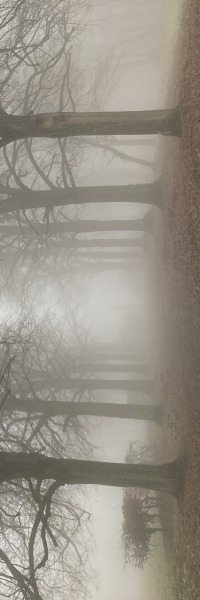
\includegraphics{./img/outro-01.jpg}

\bookmarksetup{startatroot}

\hypertarget{inferenz}{%
\chapter{Inferenz}\label{inferenz}}

\begin{figure}

{\centering 
\includegraphics[width=0.1\textwidth,height=\textheight]{./img/Golem_hex.png}

}

\caption{Bayes:Start!}

\end{figure}

\hypertarget{lernsteuerung}{%
\section{Lernsteuerung}\label{lernsteuerung}}

\hypertarget{lernziele-1}{%
\subsection{Lernziele}\label{lernziele-1}}

Nach Absolvieren des jeweiligen Kapitels sollen folgende Lernziele
erreicht sein.

Sie können \ldots{}

\begin{itemize}
\tightlist
\item
  die Definition von Inferenzstatistik sowie Beispiele für
  inferenzstatistische Fragestellungen nennen
\item
  zentrale Begriffe nennen und in Grundzügen erklären
\item
  den Nutzen von Inferenzstatistik nennen
\item
  erläutern, in welchem Zusammenhang Ungewissheit zur Inferenzstatistik
  steht
\item
  auch anhand von Beispielen erklären, was ein statistisches Modell ist
\item
  die Grundkonzepte der Regression angeben
\item
  Unterschiede zwischen klassischer und Bayes-Inferenz benennen
\item
  Vor- und Nachteile der klassischen vs.~Bayes-Inferenz diskutieren
\item
  Die grundlegende Herangehensweise zur Berechnung des p-Werts informell
  erklären können
\end{itemize}

\hypertarget{begleitvideos}{%
\subsection{Begleitvideos}\label{begleitvideos}}

\begin{itemize}
\tightlist
\item
  \href{https://youtu.be/gcwWwBy0kPI}{Video zur Inferenz, Teil 1}
\item
  \href{https://https://youtu.be/QNMVi6IqQ90}{Video zur Inferenz, Teil
  2}
\end{itemize}

\hypertarget{wozu-ist-statistik-uxfcberhaupt-da}{%
\section{Wozu ist Statistik überhaupt
da?}\label{wozu-ist-statistik-uxfcberhaupt-da}}

Ja, diese Frage haben Sie sich auch schon mal gestellt?

Abb. Abbildung~\ref{fig-goals} gibt einen Überblick über die Ziele der
Statistik.

\begin{figure}

{\centering 

\begin{figure}[H]

{\centering 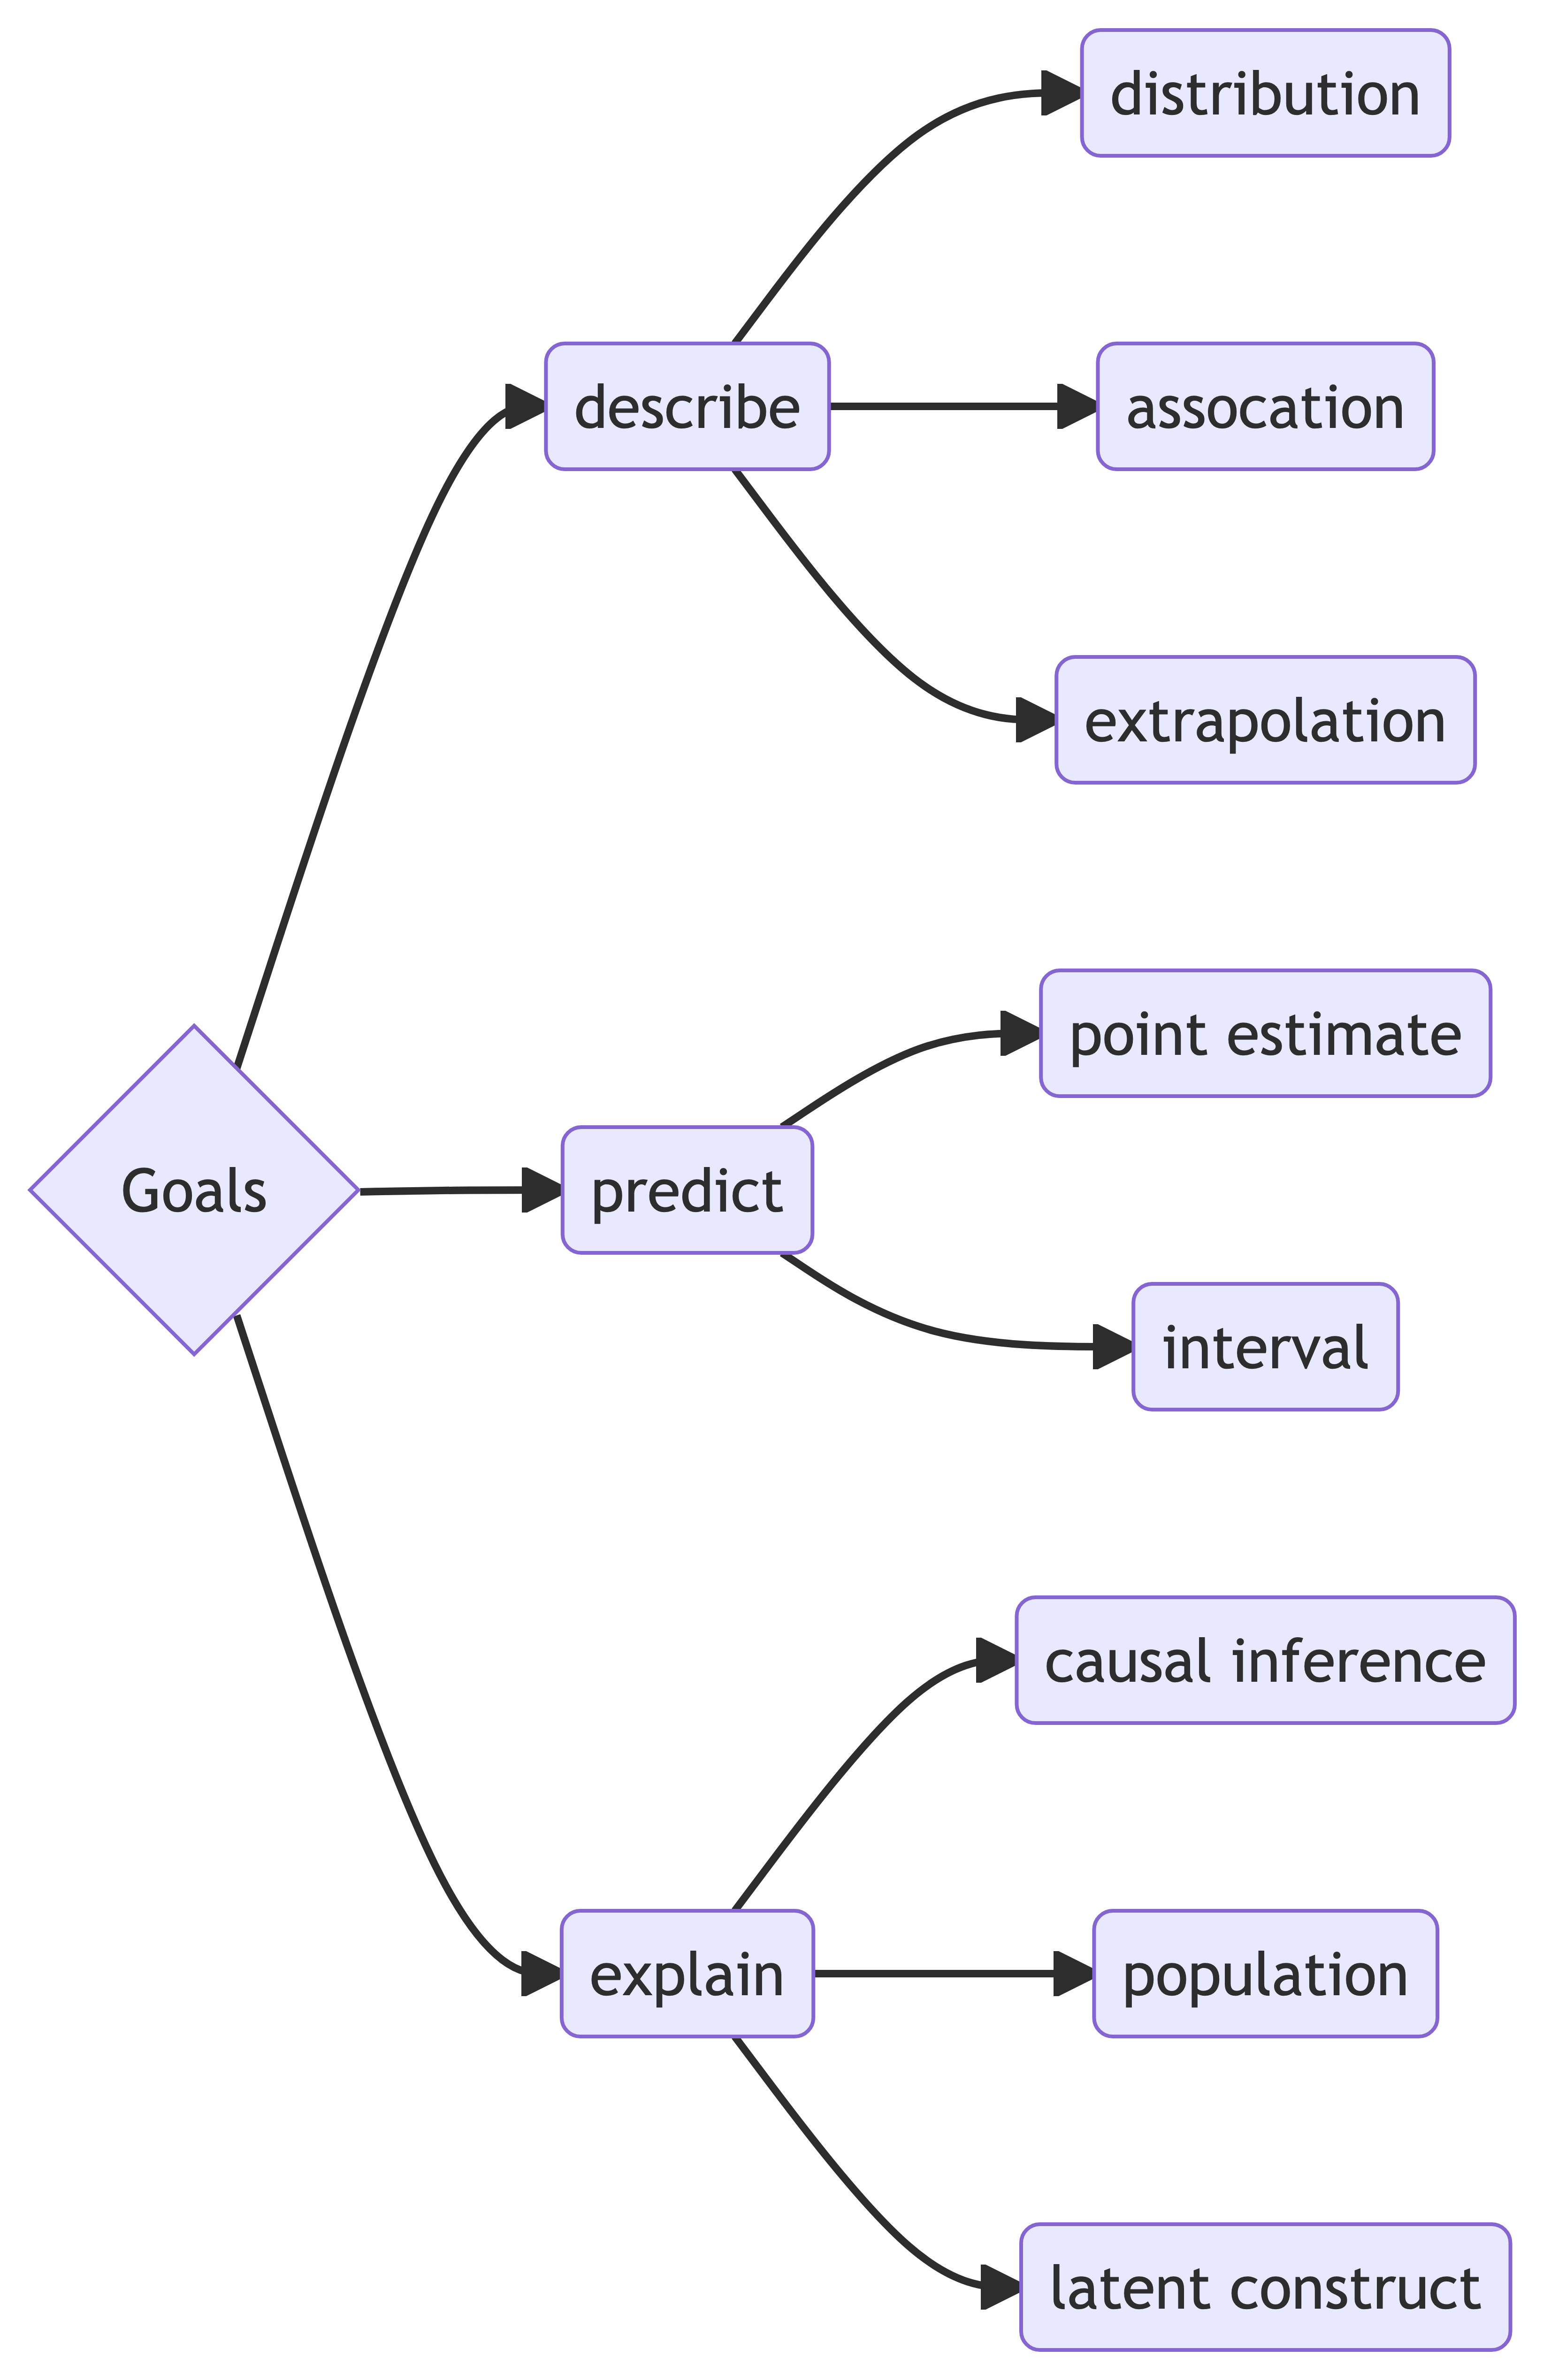
\includegraphics[width=4.29in,height=6.6in]{./Inferenz_files/figure-latex/mermaid-figure-1.png}

}

\end{figure}

}

\caption{\label{fig-goals}A taxonomy of statistical goals}

\end{figure}

\begin{tcolorbox}[enhanced jigsaw, colframe=quarto-callout-note-color-frame, breakable, titlerule=0mm, left=2mm, colbacktitle=quarto-callout-note-color!10!white, opacityback=0, colback=white, opacitybacktitle=0.6, toptitle=1mm, rightrule=.15mm, toprule=.15mm, bottomrule=.15mm, bottomtitle=1mm, title=\textcolor{quarto-callout-note-color}{\faInfo}\hspace{0.5em}{Hinweis}, leftrule=.75mm, arc=.35mm, coltitle=black]

Ziele existieren nicht ``in echt'' in der Welt. Wir denken sie uns aus.
Ziele haben also keine ontologische Wirklichkeit, sie sind
epistemologische Dinge (existieren nur in unserem Kopf). Das heißt, dass
man sich nach Beliebem Ziele ausdenken kann. Allerdings hülfe es, wenn
man andere Menschen vom Nutzen der eigenen Ideen überzeugen kann.

\end{tcolorbox}

\hypertarget{was-ist-inferenz}{%
\section{Was ist Inferenz?}\label{was-ist-inferenz}}

\hypertarget{inferenz-als-generalisieren}{%
\subsection{Inferenz als
Generalisieren}\label{inferenz-als-generalisieren}}

Statistische Inferenz sieht sich drei ``Herausforderungen'' gegenüber,
laut Gelman, Hill, und Vehtari (2021), Kap. 1.1. Diese betreffen das
Schließen (oder Generalisieren) vom Einzelfall auf das Allgemeine:

\begin{enumerate}
\def\labelenumi{\arabic{enumi}.}
\tightlist
\item
  Von der Stichprobe aus die Grundgesamtheit (Population)
\item
  Von der Experimental- auf die Kontrollgruppe (Kausalinferenz)
\item
  Von einem Messwert auf das zugrundeliegende Konstrukt
\end{enumerate}

In diesem Kurs beschäftigen wir uns mit den ersten beiden
Herausforderungen.

\begin{tcolorbox}[enhanced jigsaw, colframe=quarto-callout-important-color-frame, breakable, titlerule=0mm, left=2mm, colbacktitle=quarto-callout-important-color!10!white, opacityback=0, colback=white, opacitybacktitle=0.6, toptitle=1mm, rightrule=.15mm, toprule=.15mm, bottomrule=.15mm, bottomtitle=1mm, title=\textcolor{quarto-callout-important-color}{\faExclamation}\hspace{0.5em}{Wichtig}, leftrule=.75mm, arc=.35mm, coltitle=black]

Statistische Inferenz hat zum Ziel, vom Teil aufs Ganze zu schließen,
bzw. vom Konrketen auf das Abstrakte.

\end{tcolorbox}

\hypertarget{stichprobe-vs.-population}{%
\section{Stichprobe vs.~Population}\label{stichprobe-vs.-population}}

Nehmen wir an, wir möchten herausfinden, wie groß der Anteil der R-Fans
an der Population der Studierenden ist. Den Anteil der F-Fans bezeichnen
wir der Einfachheit halber hier mit \texttt{A}\footnote{\sout{Meistens}
  Manchmal darf man bei der Statistik nicht nach einem tieferen Sinn
  suchen. Ist Statistik eine Art moderne Kunst?}.

Das \emph{Grundproblem der Inferenzstatistik} ist, dass wir an Aussagen
zur Grundgesamtheit interessiert sind, aber nur eine Stichprobe, also
einen Ausschnitt oder eine Teilmenge der Grundgesamtheit vorliegen
haben.

Wir müssen also den Anteil der R-Fans auf Basis des Anteils in der
Stichprobe für die Grundgesamtheit schließen: Wir verallgemeinern oder
generalisieren von der Stichprobe auf die Grundgesamtheit, s. Abb.
Abbildung~\ref{fig-pop-sample}.

\begin{figure}

\begin{minipage}[t]{0.50\linewidth}

{\centering 

\raisebox{-\height}{

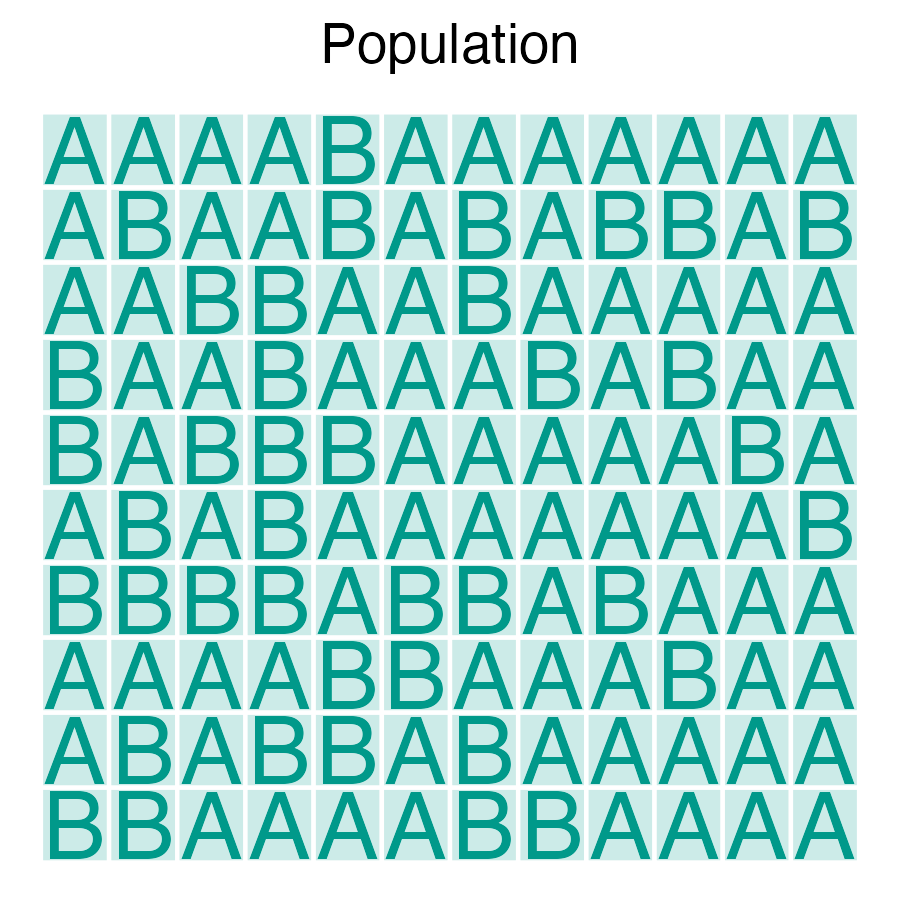
\includegraphics{./img/pvoll.png}

}

}

\subcaption{\label{fig-pop}Population}
\end{minipage}%
%
\begin{minipage}[t]{0.50\linewidth}

{\centering 

\raisebox{-\height}{

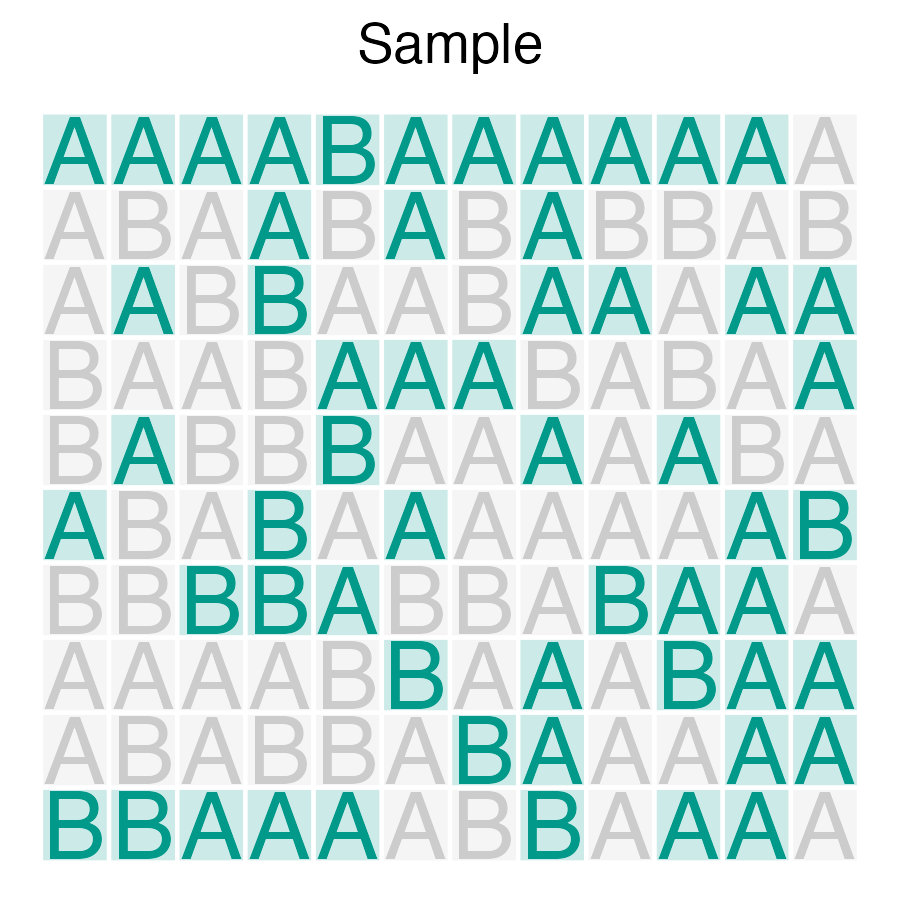
\includegraphics{./img/psti.png}

}

}

\subcaption{\label{fig-sample}Sample}
\end{minipage}%

\caption{\label{fig-pop-sample}Population vs.~sample (Image credit:
Karsten Luebke)}

\end{figure}

Häufig ist das praktische Vorgehen recht simpel: Ah, in unserer
Stichprobe sind 42\% R-Fans!\footnote{Mancheiner hätte mit mehr
  gerechnet}. Man schreibt: \(p = 0.42\) (\texttt{p} wie
\texttt{proportion}). Die Stichprobe sei repräsentativ für die
Grundgesamtheit aller Studierender. Messerscharf schließen wir: In der
Grundgesamtheit ist der Anteil der R-Fans auch 42\%, \(\pi=0.42\).

\hypertarget{deskriptiv--vs.-inferenzstatistik}{%
\subsection{Deskriptiv-
vs.~Inferenzstatistik}\label{deskriptiv--vs.-inferenzstatistik}}

Statistik gibt es in zwei Geschmacksrichtungen, könnte man sagen:
Deskriptiv- und Inferenzstatistik, s. Abb. Abbildung~\ref{fig-inf1}.
Einteilungen in Schubladen existieren nicht auf der Welt, sondern in
unserem Kopf: Sie besitzen keine ontologische Realität, sondern eine
epistemologische. Sie sind frei, sich andere Einteilungen der Statistik
auszudenken. Es hilft allerdings, wenn man andere Menschen vom Wert
seiner Idee überzeugen kann.

\begin{figure}

{\centering 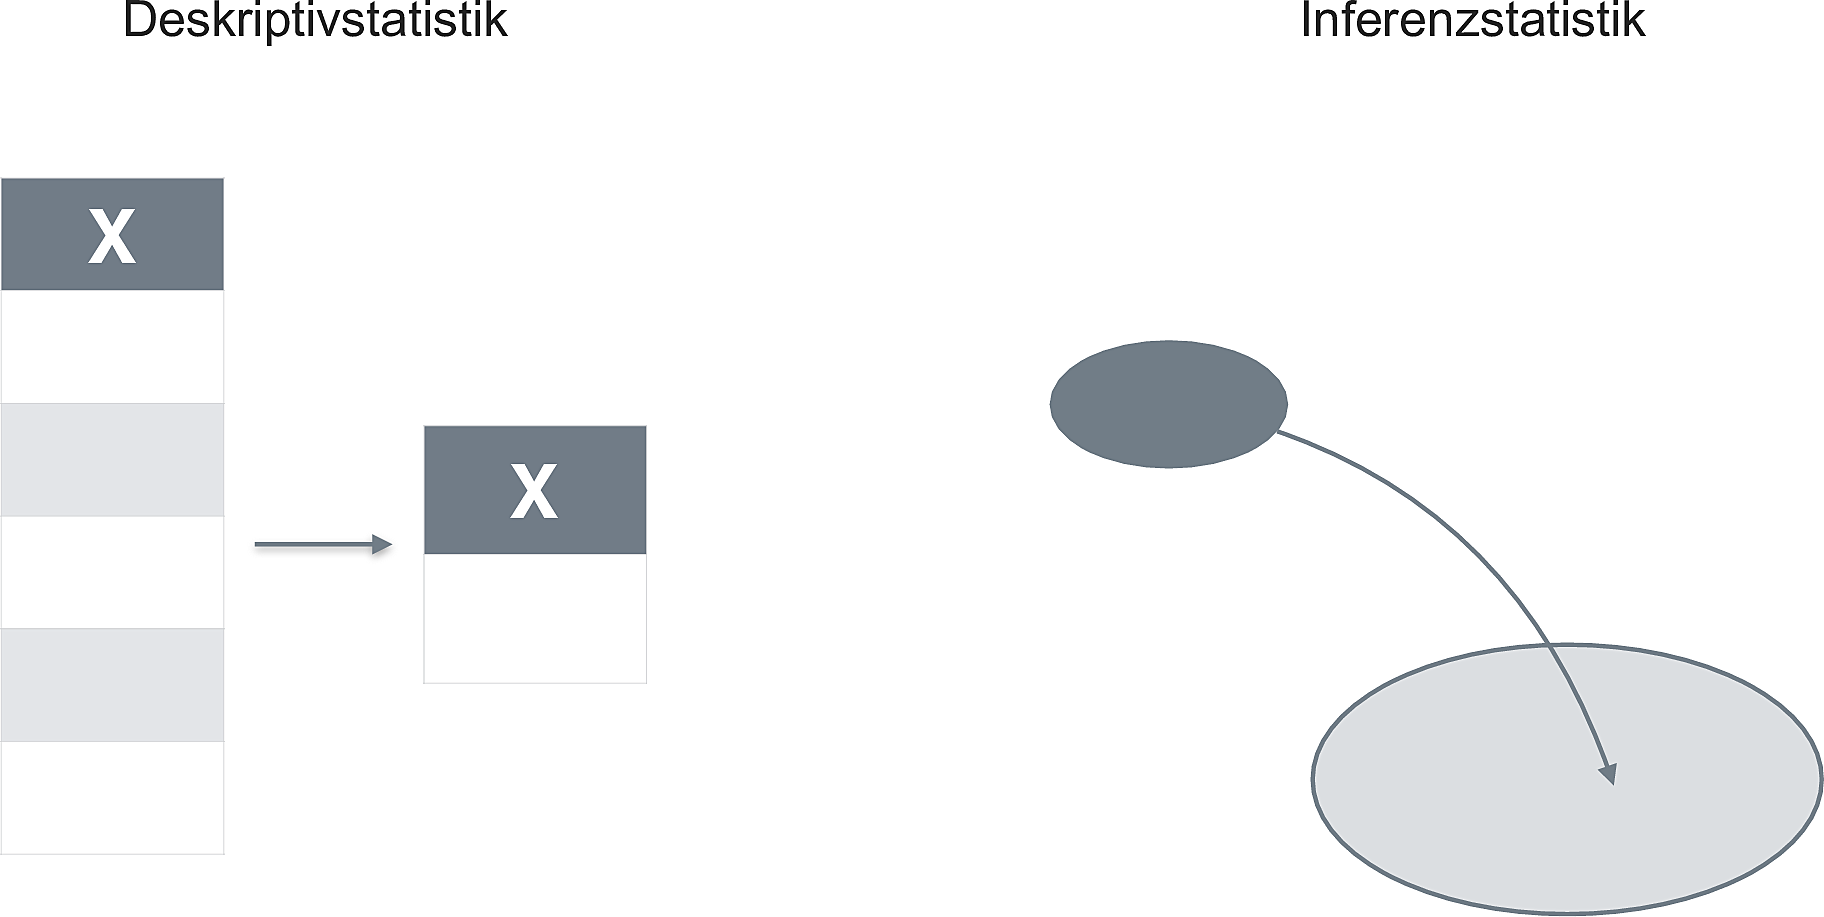
\includegraphics[width=0.7\textwidth,height=\textheight]{./img/desk_vs_inf-crop.png}

}

\caption{\label{fig-inf1}Deskriptiv- vs.~Inferenzstatistik}

\end{figure}

\emph{Deskriptivstastistik} fasst Stichprobenmerkmale zu Kennzahlen
(Statistiken) zusammen.

\emph{Inferenzstatistik} schließt von Statistiken auf Parameter
(Kennzahlen von Grundgesamtheiten).

🏋 Schließen Sie die Augen und zeichnen Sie obiges Diagramm!

\hypertarget{wozu-ist-die-inferenstatistik-gut}{%
\subsection{Wozu ist die Inferenstatistik
gut?}\label{wozu-ist-die-inferenstatistik-gut}}

\begin{tcolorbox}[enhanced jigsaw, colframe=quarto-callout-note-color-frame, breakable, titlerule=0mm, left=2mm, colbacktitle=quarto-callout-note-color!10!white, opacityback=0, colback=white, opacitybacktitle=0.6, toptitle=1mm, rightrule=.15mm, toprule=.15mm, bottomrule=.15mm, bottomtitle=1mm, title=\textcolor{quarto-callout-note-color}{\faInfo}\hspace{0.5em}{Hinweis}, leftrule=.75mm, arc=.35mm, coltitle=black]

Inferenz bedeutet Schließen; auf Basis von vorliegenden Wissen wird
neues Wissen generiert.

\end{tcolorbox}

Inferenzstatistik ist ein Verfahren, das mathematische Modelle (oft aus
der Stochastik) verwendet, um ausgehend von einer bestimmten Datenlage,
die eine Stichprobe einer Grundgesamtheit darstellt, allgemeine Schlüsse
zu ziehen.

🏋️️ Heute Nacht vor dem Schlafen wiederholen Sie die Definition. Üben Sie
jetzt schon mal.

\hypertarget{deskriptiv--und-inferenzstatistik-gehen-hand-in-hand}{%
\subsection{Deskriptiv- und Inferenzstatistik gehen Hand in
Hand}\label{deskriptiv--und-inferenzstatistik-gehen-hand-in-hand}}

Für jede beliebige Statistik (Kennzahl von Stichprobendaten) kann man
die Methoden der Inferenzstatistik verwenden, s. Tabelle
Tabelle~\ref{tbl-kennwerte}.

\hypertarget{tbl-kennwerte}{}
\begin{longtable}[]{@{}lll@{}}
\caption{\label{tbl-kennwerte}Bezeichnungen für
Kennwerte}\tabularnewline
\toprule()
Kennwert & Stichprobe & Grundgesamtheit \\
\midrule()
\endfirsthead
\toprule()
Kennwert & Stichprobe & Grundgesamtheit \\
\midrule()
\endhead
Mittelwert & \(\bar{X}\) & \(\mu\) \\
Streuung & \(sd\) & \(\sigma\) \\
Anteil & \(p\) & \(\pi\) \\
Korrelation & \(r\) & \(\rho\) \\
Regression & \(b\) & \(\beta\) \\
\bottomrule()
\end{longtable}

Für Statistiken (Daten einer Stichprobe) verwendet man
\emph{lateinische} Buchstaben; für Parameter (Population) verwendet man
\emph{griechische} Buchstaben.

🏋️ Geben Sie die griechischen Buchstaben für typische Statistiken an!

\hypertarget{schuxe4tzen-von-parametern-einer-grundgesamtheit}{%
\subsection{Schätzen von Parametern einer
Grundgesamtheit}\label{schuxe4tzen-von-parametern-einer-grundgesamtheit}}

Meist begnügt man sich beim Analysieren von Daten nicht mit Aussagen für
eine Stichprobe, sondern will auf eine Grundgesamtheit verallgemeinern.

Leider sind die Parameter einer Grundgesamtheit zumeist unbekannt, daher
muss man sich mit \emph{Schätzungen} begnügen.

Schätzwerte werden mit einem ``Dach'' über dem Kennwert gekennzeichnet,
z.B.

\begin{longtable}[]{@{}llll@{}}
\toprule()
Kennwert & Stichprobe & Grundgesamtheit & Schätzwert \\
\midrule()
\endhead
Mittelwert & \(\bar{X}\) & \(\mu\) & \(\hat{\mu}\) \\
Streuung & \(sd\) & \(\sigma\) & \(\hat{\sigma}\) \\
Anteil & \(p\) & \(\pi\) & \(\hat{\pi}\) \\
Korrelation & \(r\) & \(\rho\) & \(\hat{\rho}\) \\
Regression & \(b\) & \(\beta\) & \(\hat{\beta}\) \\
\bottomrule()
\end{longtable}

\hypertarget{beispiele-fuxfcr-inferenzstatistische-fragestellungen}{%
\subsection{Beispiele für inferenzstatistische
Fragestellungen}\label{beispiele-fuxfcr-inferenzstatistische-fragestellungen}}

Sie testen zwei Varianten Ihres Webshops (V1 und V2), die sich im
Farbschema unterscheiden und ansonsten identisch sind: Hat das
Farbschema einen Einfluss auf den Umsatz?

\begin{itemize}
\item
  Dazu vergleichen Sie den mittleren Umsatz pro Tag von V1 vs.~V2,
  \(\bar{X}_{V1}\) und \(\bar{X}_{V2}\).
\item
  Die Mittelwerte unterscheiden sich etwas,
  \(\bar{X}_{V1} > \bar{X}_{V2}\)
\item
  Sind diese Unterschiede ``zufällig'' oder ``substanziell''? Gilt also
  \(\mu_{V1} > \mu_{V2}\) oder gilt \(\mu_{V1} \le \mu_{V2}\)?
\item
  Wie groß ist die Wahrscheinlichkeit\footnote{oft mit \emph{Pr} oder
    \emph{p} abgekürzt, für \emph{probability}}
  \(Pr(\mu_{V1} > \mu_{V2})\)?
\end{itemize}

🏋️ \emph{Predictive Maintenance} ist ein Anwendungsfeld
inferenzstatistischer Modellierung. Lesen Sie dazu S. 3
\href{https://www.rolandberger.com/publications/publication_pdf/roland_berger_vdma_predictive_maintenance_d_1.pdf}{dieses
Berichts}!

\hypertarget{modellieren}{%
\section{Modellieren}\label{modellieren}}

\hypertarget{modellieren-als-grundraster-des-erkennens}{%
\subsection{Modellieren als Grundraster des
Erkennens}\label{modellieren-als-grundraster-des-erkennens}}

In der Wissenschaft - wie auch oft in der Technik, Wirtschaft oder im
Alltag - betrachtet man einen Teil der Welt näher, meist mit dem Ziel,
eine Entscheidung zu treffen, was man tun wird oder mit dem Ziel, etwas
zu lernen.

Nun ist die Welt ein weites Feld. Jedes Detail zu berücksichtigen ist
nicht möglich. Wir müssen die Sache vereinfachen: Alle Informationen
ausblenden, die nicht zwingend nötig sind. Aber gleichzeitig die
Strukturelemente der wirklichen Welt, die für unsere Fragestellung
zentral ist, beibehalten.

Dieses Tun nennt man \emph{Modellieren}: Man erstellt sich ein Modell.

\begin{tcolorbox}[enhanced jigsaw, colframe=quarto-callout-important-color-frame, breakable, titlerule=0mm, left=2mm, colbacktitle=quarto-callout-important-color!10!white, opacityback=0, colback=white, opacitybacktitle=0.6, toptitle=1mm, rightrule=.15mm, toprule=.15mm, bottomrule=.15mm, bottomtitle=1mm, title=\textcolor{quarto-callout-important-color}{\faExclamation}\hspace{0.5em}{Wichtig}, leftrule=.75mm, arc=.35mm, coltitle=black]

Ein Modell ist ein vereinfachtes Abbild der Wirklichkeit.

\end{tcolorbox}

Auf die Statistik bezogen heißt das, dass man einen Datensatz zu
zusammenfasst, dass man das Wesentliche erkennt. Was ist das
``Wesentliche''? Meist interessiert man sich für die Ursachen eines
Phänomens? Etwa: ``Wie kommt es bloß, dass ich ohne zu lernen die
Klausur so gut bestanden habe?''\footnote{Das ist natürlich nur ein
  fiktives, komplett unrealistisches Beispiel, das auch unklaren
  Ursachen den Weg auf diese Seite gefunden hat.} Noch allgemeiner ist
vom häufig am Zusammenhang von \texttt{X} und \texttt{Y} interessiert,
s. Abbildung~\ref{fig-xy}, linker Teil, die ein Sinnbild eines
statistischen Modells widergibt.

\begin{figure}

{\centering 

\begin{figure}[H]

{\centering 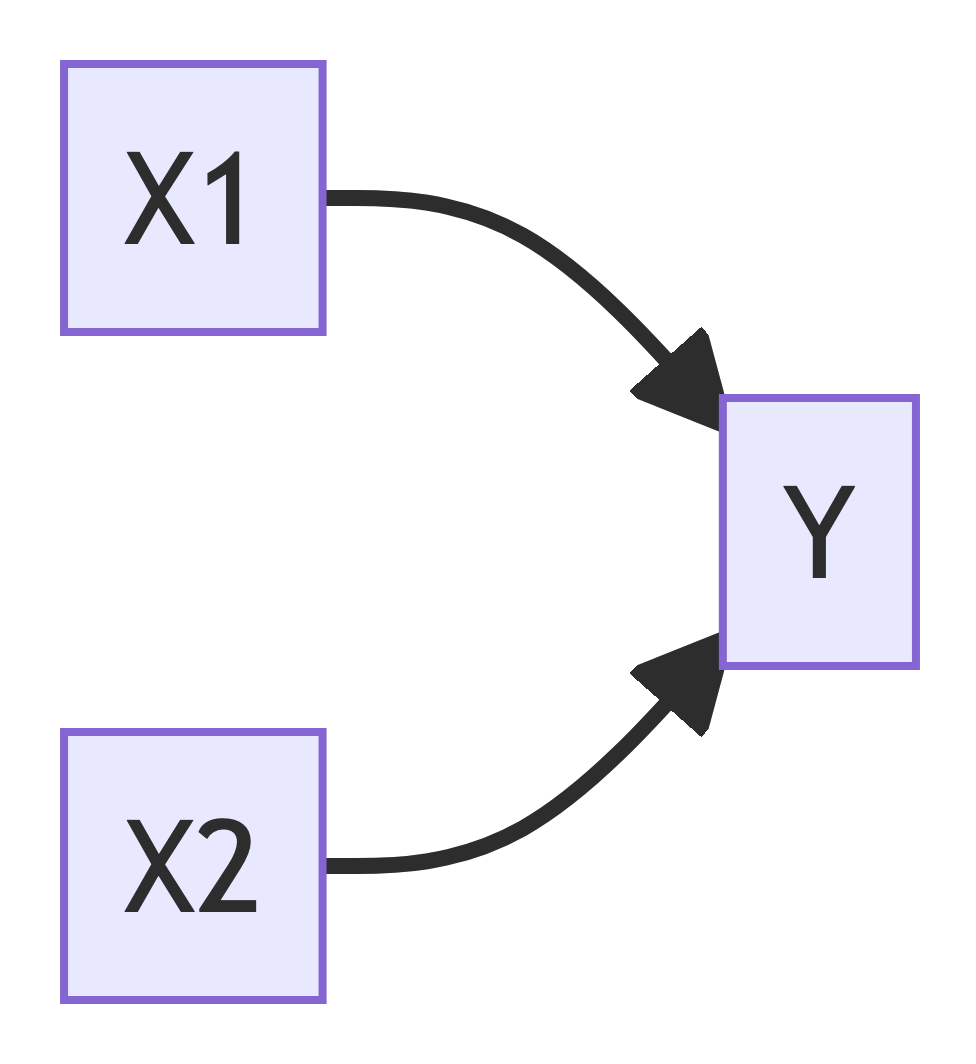
\includegraphics[width=1.36in,height=2.26in]{./Inferenz_files/figure-latex/mermaid-figure-3.png}

}

\end{figure}

}

\caption{\label{fig-xy}oben: Sinnbild eines statistischen Modells;
unten: Sinnbild eines statistischen Modells, mit zwei Inputvariablen
(Ursachen)}

\end{figure}

Das Diagramm hat Sie nicht so vom Hocker? Okay, ein statistisches Modell
kann natürlich komplexer sein, z.B. wie in Abb. Abbildung~\ref{fig-xy},
rechter Teil, dargestellt.

Es hört sich zugspitzt an, aber eigentlich ist fast alles Modellieren:
Wenn man den Anteil der R-Fans in einer Gruppe Studierender ausrechnet,
macht man sich ein Modell: man vereinfacht diesen Ausschnitt der
Wirklichkeit anhand einer statistischen Kennzahl, die das
forschungsleitende Interesse zusammenfasst.

\hypertarget{vertiefung}{%
\subsection{Vertiefung}\label{vertiefung}}

Lesen Sie die Einführung zum Thema Modellieren bei Poldrack (2022) (Kap.
5.1).

\begin{tcolorbox}[enhanced jigsaw, colframe=quarto-callout-note-color-frame, breakable, titlerule=0mm, left=2mm, colbacktitle=quarto-callout-note-color!10!white, opacityback=0, colback=white, opacitybacktitle=0.6, toptitle=1mm, rightrule=.15mm, toprule=.15mm, bottomrule=.15mm, bottomtitle=1mm, title=\textcolor{quarto-callout-note-color}{\faInfo}\hspace{0.5em}{Hinweis}, leftrule=.75mm, arc=.35mm, coltitle=black]

Nutzen Sie die Übersetzungsfunktion Ihres Browsers, wenn Sie einen
englischen Text lieber auf Deutsch lesen wollen. Oder einen deutschen
lieber auf Englisch.

\end{tcolorbox}

\hypertarget{regression}{%
\section{Regression}\label{regression}}

Einflussreiche Leute schwören auf die Regressionsanalyse
(Abbildung~\ref{fig-gandalf}).

\begin{figure}

{\centering 
\includegraphics[width=0.5\textwidth,height=\textheight]{./img/einring.jpg}

}

\caption{\label{fig-gandalf}One regression}

\end{figure}

\hypertarget{regression-zum-modellieren}{%
\subsection{Regression zum
Modellieren}\label{regression-zum-modellieren}}

Die Regression ist eine Art Schweizer Taschenmessen: Für vieles gut
einsetzbar.

Anstelle von vielen verschiedenen Verfahren des statistischen
Modellierens kann man (fast) immer die Regression verwenden. Das ist
nicht nur einfacher, sondern auch schöner. Wir werden im Folgenden stets
die Regression zum Modellieren verwenden.

Dann wenden wir die Methoden der Inferenz auf die Kennzahlen der
Regression an.

\begin{tcolorbox}[enhanced jigsaw, colframe=quarto-callout-note-color-frame, breakable, titlerule=0mm, left=2mm, colbacktitle=quarto-callout-note-color!10!white, opacityback=0, colback=white, opacitybacktitle=0.6, toptitle=1mm, rightrule=.15mm, toprule=.15mm, bottomrule=.15mm, bottomtitle=1mm, title=\textcolor{quarto-callout-note-color}{\faInfo}\hspace{0.5em}{Hinweis}, leftrule=.75mm, arc=.35mm, coltitle=black]

Regression + Inferenz = 💖

\end{tcolorbox}

Alternativ zur Regression könnte man sich in den Wald der statistischen
Verfahren begeben,
\href{https://web.archive.org/web/20091029162244/http://www.wiwi.uni-muenster.de/ioeb/en/organisation/pfaff/stat_overview_table.html}{wie
hier von der Uni Münster als Ausschnitt (!) aufgeführt}.

Auf dieser Basis kann man meditieren, welches statistischen Verfahren
man für eine bestimmte Fragestellung verwenden sollte, s. Abb.
Abbildung~\ref{fig-choose-test}.

\begin{figure}

{\centering 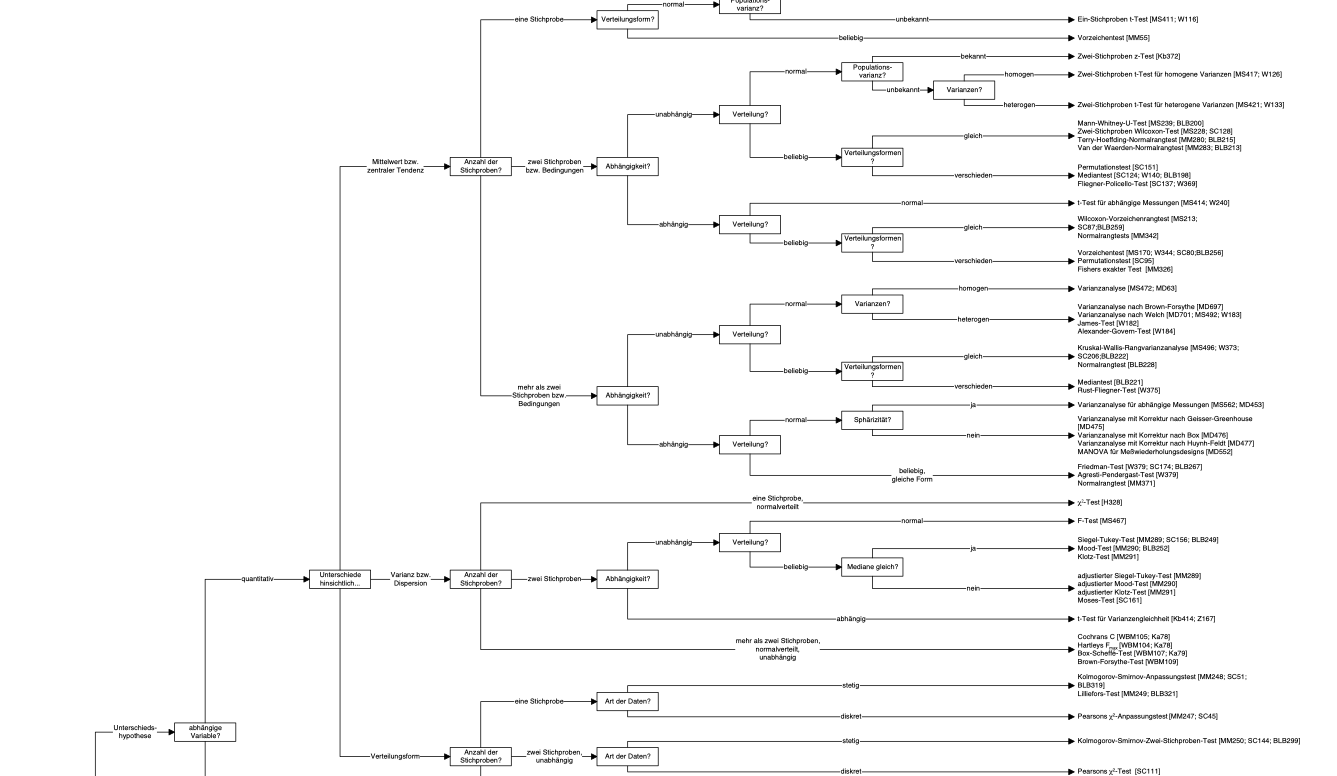
\includegraphics{./img/choose-test.png}

}

\caption{\label{fig-choose-test}Wähle deine Statistik mit Bedacht}

\end{figure}

\hypertarget{viele-statistische-verfahren-sind-spezialfuxe4lle-der-regression}{%
\subsection{Viele statistische Verfahren sind Spezialfälle der
Regression}\label{viele-statistische-verfahren-sind-spezialfuxe4lle-der-regression}}

Wie Jonas Kristoffer Lindeløv uns erklärt, sind viele statistische
Verfahren, wie der sog. t-Test Spezialfälle der Regression, s. Abb.
Abbildung~\ref{fig-lindeloev}.

\begin{figure}

{\centering 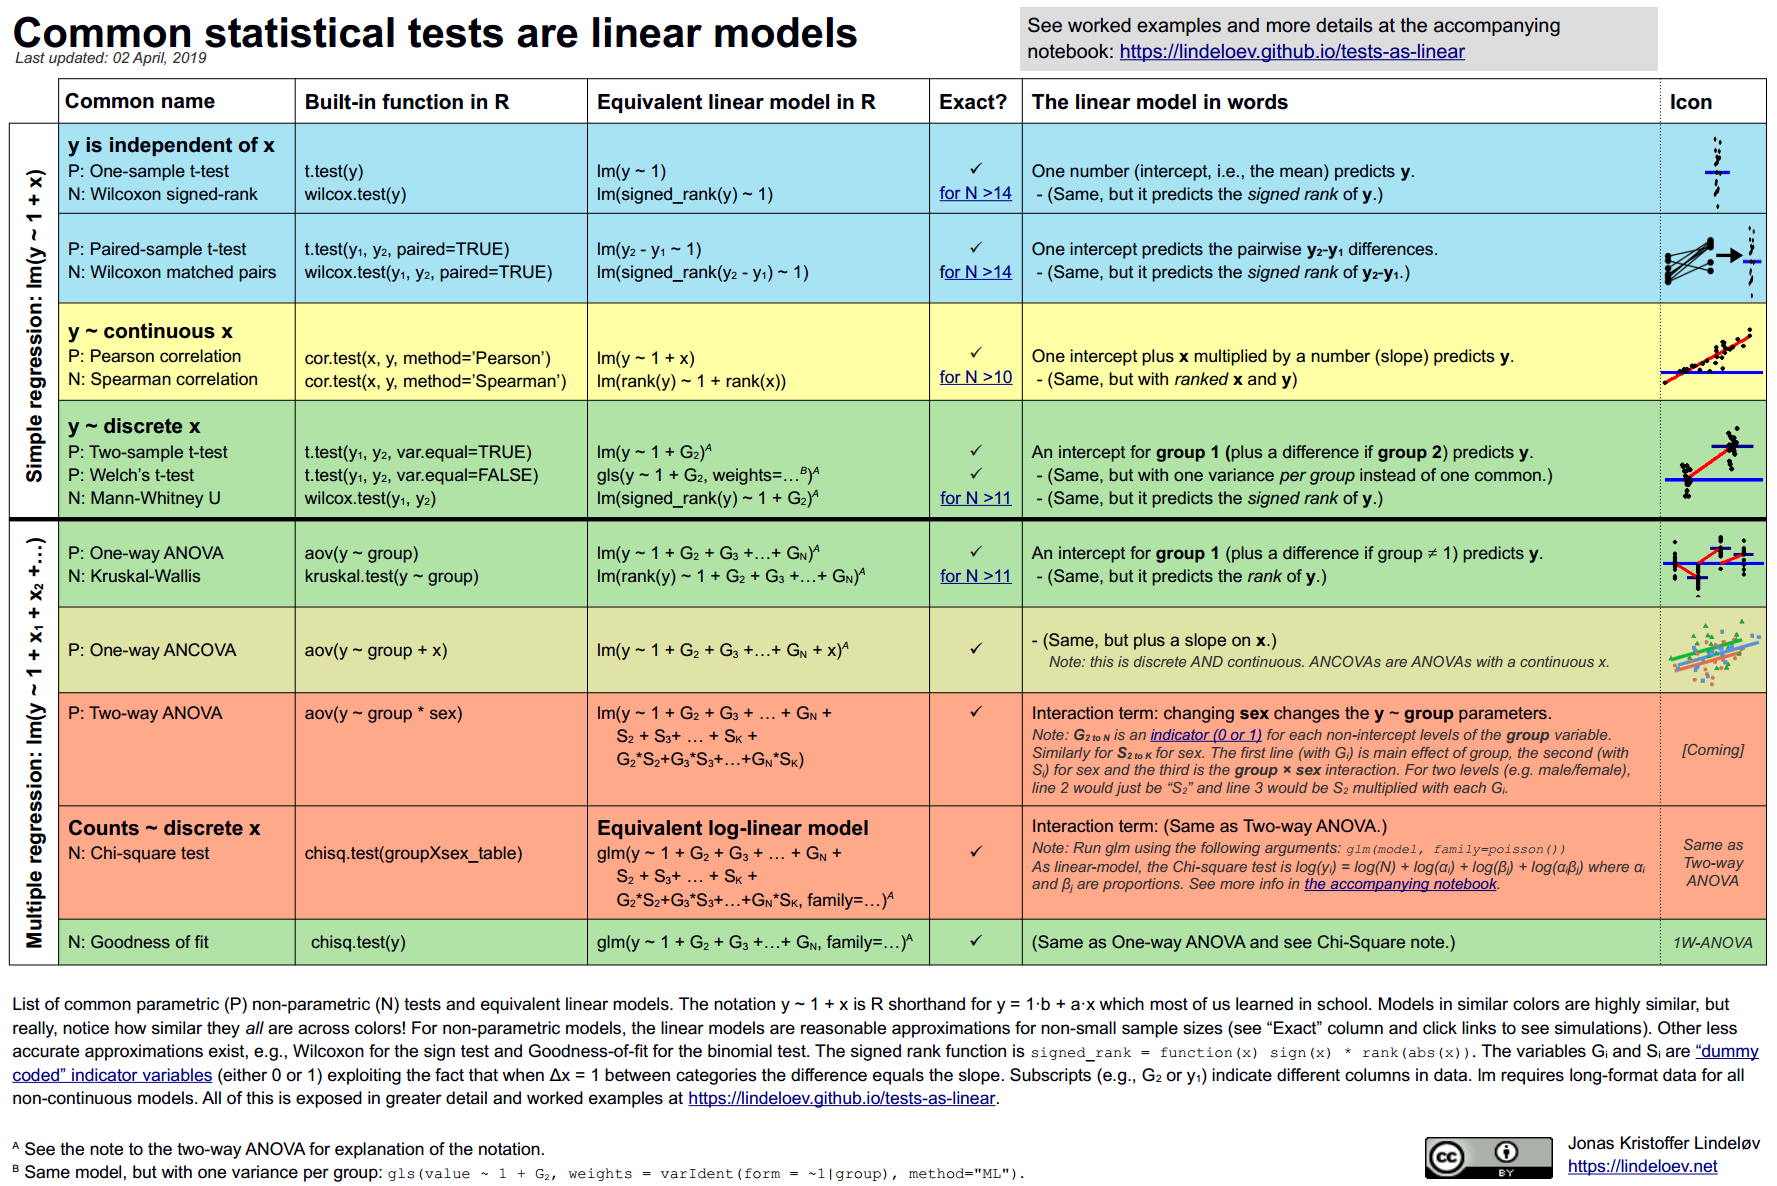
\includegraphics{./img/linear_tests_cheat_sheet.png}

}

\caption{\label{fig-lindeloev}Common statistical tests as linear models}

\end{figure}

\hypertarget{in-voller-pracht}{%
\subsection{In voller Pracht}\label{in-voller-pracht}}

Hier ist die Regressionsgleichung in voller Pracht; Abb.
Abbildung~\ref{fig-regr-rules}.

\[y = \beta_0 + \beta_1 x_1 + \ldots + \beta_k x_k + \epsilon\]

Anhan der Gleichung erkennt man auch, warum man von einem \emph{linearen
Modell} spricht: Y wird als gewichteter Mittelwert mehrerer Summanden
berechnet. Dabei wird X nicht mit ``fortgeschrittenen'' Transformationen
wie Quadradieren oder Exponenzieren beglückt, sondern nur mit den
Regressiongewichten multipliziert.

\begin{figure}

{\centering 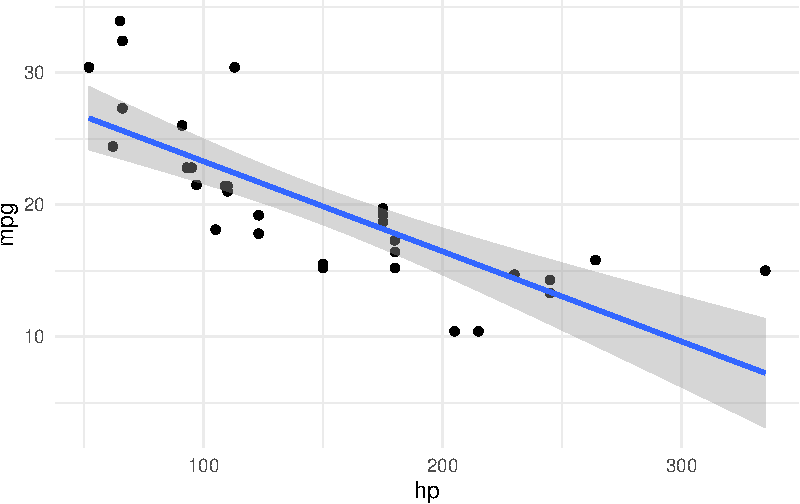
\includegraphics{./Inferenz_files/figure-pdf/fig-regr-rules-1.pdf}

}

\caption{\label{fig-regr-rules}Die Regressionsgerade in voller Pracht}

\end{figure}

\hypertarget{unsicherheit}{%
\section{Unsicherheit}\label{unsicherheit}}

\hypertarget{inferenz-beinhaltet-unsicherheit}{%
\subsection{Inferenz beinhaltet
Unsicherheit}\label{inferenz-beinhaltet-unsicherheit}}

Inferenzstatistische Schlüsse sind mit Unsicherheit behaftet:
Schließlich kennt man nur einen Teil (die Stichprobe) eines Ganzen (die
Population), möchte aber vom Teil auf das Ganze schließen.

\begin{tcolorbox}[enhanced jigsaw, colframe=quarto-callout-important-color-frame, breakable, titlerule=0mm, left=2mm, colbacktitle=quarto-callout-important-color!10!white, opacityback=0, colback=white, opacitybacktitle=0.6, toptitle=1mm, rightrule=.15mm, toprule=.15mm, bottomrule=.15mm, bottomtitle=1mm, title=\textcolor{quarto-callout-important-color}{\faExclamation}\hspace{0.5em}{Wichtig}, leftrule=.75mm, arc=.35mm, coltitle=black]

Nichts Genaues weiß man nicht: Schließt man von einem Teil auf das
Ganze, so geschieht das unter Unsicherheit. Man spricht von
Ungewissheit, da man die Unsicherheit das Wissen über das Ganze
betrifft.

\end{tcolorbox}

Schließt man etwa, dass in einer Grundgesamtheit der Anteil der R-Fans
bei 42\% liegt, so geschieht das unter Unsicherheit. Man ist sich nicht
sicher, dass es wirklich 42\% in der Population sind - und nicht etwa
etwas mehr oder etwas weniger. Schließlich hat man \emph{nicht} die
ganze Population gesehen bzw. vermessen. \emph{Sicher} ist man sich
hingegen für die Stichprobe (Messfehler einmal ausgeblendet).

Zur Bemessung der Unsicherheit (Ungewissheit) bedient man sich der
Wahrscheinlichkeitsrechnung (wo immer möglich).

Die Wahrscheinlichkeitstheorie bzw. -rechnung wird auch als die
Mathematik des Zufalls bezeichnet.

\begin{tcolorbox}[enhanced jigsaw, colframe=quarto-callout-note-color-frame, breakable, titlerule=0mm, left=2mm, colbacktitle=quarto-callout-note-color!10!white, opacityback=0, colback=white, opacitybacktitle=0.6, toptitle=1mm, rightrule=.15mm, toprule=.15mm, bottomrule=.15mm, bottomtitle=1mm, title=\textcolor{quarto-callout-note-color}{\faInfo}\hspace{0.5em}{Hinweis}, leftrule=.75mm, arc=.35mm, coltitle=black]

Unter einem zufälligen Ereignis (random) verstehen wir ein Ereignis, das
nicht (komplett) vorherzusehen ist, wie etwa die Augenzahl Ihres
nächsten Würfelwurfs. Zufällig bedeutet nicht (zwangsläufig), dass das
Ereignisse keine Ursachen besitzt. So gehorchen die Bewegungen eines
Würfels den Gesetzen der Physik, nur sind uns diese oder die genauen
Randbedingungen nicht (ausreichend) bekannt.

\end{tcolorbox}

🏋 Welche physikalischen Randbedingungen wirken wohl auf einen Münzwurf
ein?

\hypertarget{beispiele-zur-quantifizierung-von-ungewissheit}{%
\subsection{Beispiele zur Quantifizierung von
Ungewissheit}\label{beispiele-zur-quantifizierung-von-ungewissheit}}

Aussagen mit Unsicherheit können unterschiedlich präzise formuliert
sein.

\begin{itemize}
\item
  Morgen regnet's \(\Leftrightarrow\) Morgen wird es hier mehr als 0 mm
  Niederschlag geben (\(p=97\%\)).
\item
  Methode \(A\) ist besser als Methode \(B\) \(\Leftrightarrow\) Mit
  einer Wahrscheinlichkeit von 57\% ist der Mittelwert für Methode \(A\)
  höher als für Methode \(B\).
\item
  Die Maschine fällt demnächst aus \(\Leftrightarrow\) Mit einer
  Wahrscheinlichkeit von 97\% wird die Maschine in den nächsten 1-3
  Tagen ausfallen, laut unserem Modell.
\item
  Die Investition lohnt sich \(\Leftrightarrow\) Die Investition hat
  einen Erwartungswert von 42 Euro; mit 90\% Wahrscheinlichkeit wird der
  Gewinn zwischen -10000 und 100 Euro.
\end{itemize}

🏋 Geben Sie weitere Beispiele an!

\hypertarget{zwei-arten-von-ungewissheit}{%
\subsection{Zwei Arten von
Ungewissheit}\label{zwei-arten-von-ungewissheit}}

Im Modellieren im Allgemeinen und in Regressionsmodellen im Besonderen
lassen sich (mindestens) zwei Arten von Ungewissheiten angeben, s. auch
Abb. Abbildung~\ref{fig-zwei-arten}.

\begin{enumerate}
\def\labelenumi{\arabic{enumi}.}
\item
  Wie (un)gewiss ist man sich über den Wert des Regressionsgewichts?
\item
  Wie (un)gewiss ist man sich über den Wert von Y? Schließlich könnte es
  ja Einflüsse (X) geben, die man nicht berücksichtigt hat.
\end{enumerate}

\begin{figure}

{\centering 

\begin{figure}[H]

{\centering 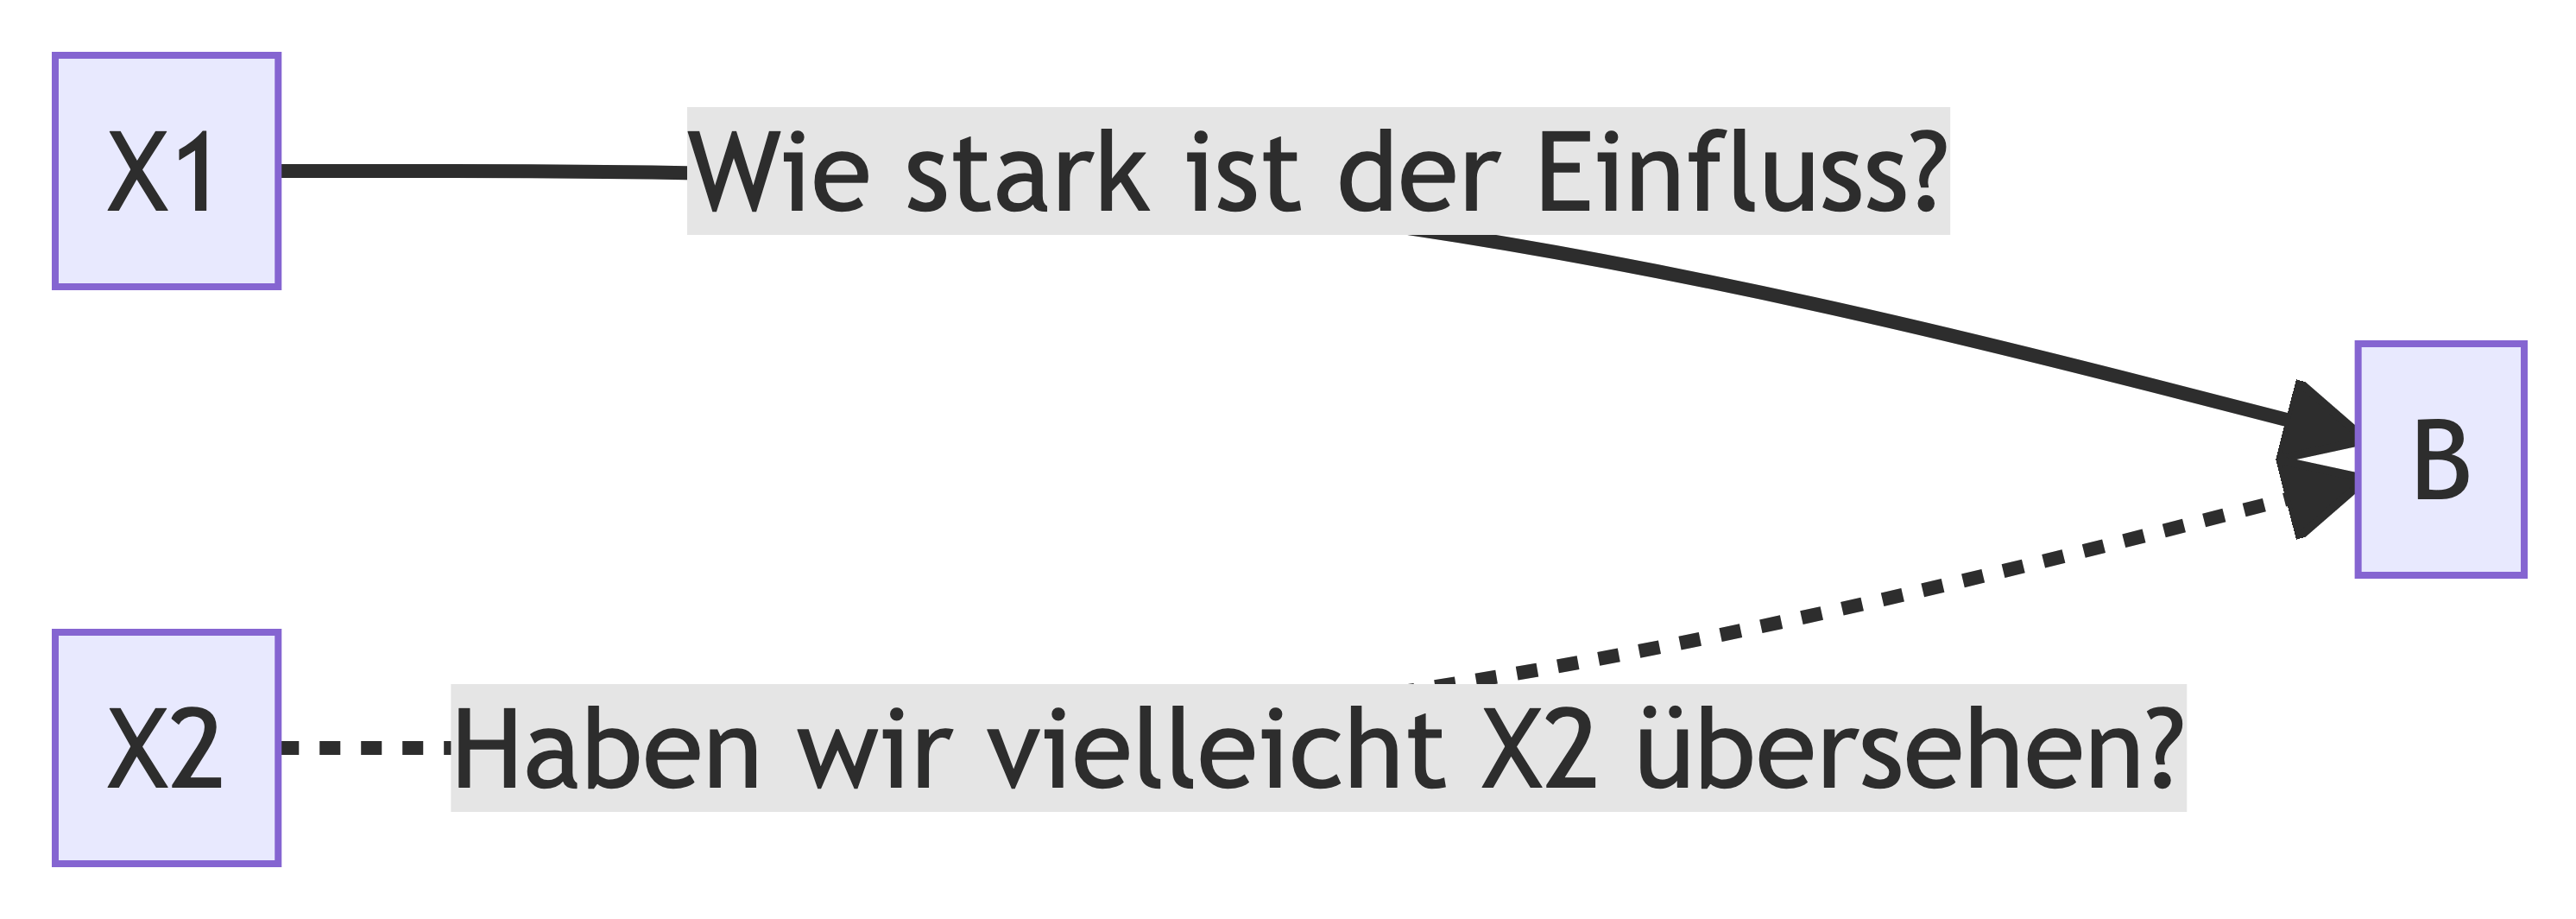
\includegraphics[width=3.89in,height=1.39in]{./Inferenz_files/figure-latex/mermaid-figure-2.png}

}

\end{figure}

}

\caption{\label{fig-zwei-arten}Zwei Arten der Ungewissheit beim
Modellieren}

\end{figure}

\hypertarget{ich-weiuxdf-was-ich-nicht-weiuxdf-ungewissheit-angeben}{%
\subsection{Ich weiß, was ich nicht weiß: Ungewissheit
angeben}\label{ich-weiuxdf-was-ich-nicht-weiuxdf-ungewissheit-angeben}}

Streng genommen ist eine Inferenz aus Angabe der Ungewissheit
(Genuaigkeit der Schätzung) wertlos. Angenommen, jemand sagt, dass sie
den Anteil der R-Fans (in der Population) auf 42\% schätzt, lässt aber
offen wie \emph{sicher} (präzise) die Schätzung ist. Wir wissen also
nicht, ob z.B. 2\% oder 82\% noch erwartbar sind. Oder ob man im
Gegenteil mit hoher Sicherheit sagen kann, die Schätzung schließt sogar
41\% oder 43\% aus.

\begin{tcolorbox}[enhanced jigsaw, colframe=quarto-callout-important-color-frame, breakable, titlerule=0mm, left=2mm, colbacktitle=quarto-callout-important-color!10!white, opacityback=0, colback=white, opacitybacktitle=0.6, toptitle=1mm, rightrule=.15mm, toprule=.15mm, bottomrule=.15mm, bottomtitle=1mm, title=\textcolor{quarto-callout-important-color}{\faExclamation}\hspace{0.5em}{Wichtig}, leftrule=.75mm, arc=.35mm, coltitle=black]

Eine Inferenz nennt man auch Schätzung. Es sollte immer die Genauigkeit
(Ungewissheit) der Schätzung angegeben werden.

\end{tcolorbox}

Im Rahmen der Regressionsanalyse schlägt sich die Ungewissheit an zwei
Stellen nieder:

\begin{enumerate}
\def\labelenumi{\arabic{enumi}.}
\tightlist
\item
  zur Lage der Regressionsgeraden (\(\beta_0\), \(\beta_1\))
\item
  zu Einflüssen (X), die unser Modell nicht kennt (\(\epsilon, \sigma\))
\end{enumerate}

\hypertarget{visualisierung-von-ungewissheit}{%
\subsection{Visualisierung von
Ungewissheit}\label{visualisierung-von-ungewissheit}}

Gibt man nur einen Punktwert an, wie 42\%, als Ergebnis einer Inferenz,
spricht man von einem \emph{Punktschätzer}. Punktschätzer beinhalten
\emph{keine Angabe} der Schätz(un)genauigkeit, s. Abb.
Abbildung~\ref{fig-punktschaetzer2}, links. Rot markiert: Die
Punktschätzung von \texttt{mpg} für \texttt{hp=200}.

\begin{figure}

{\centering 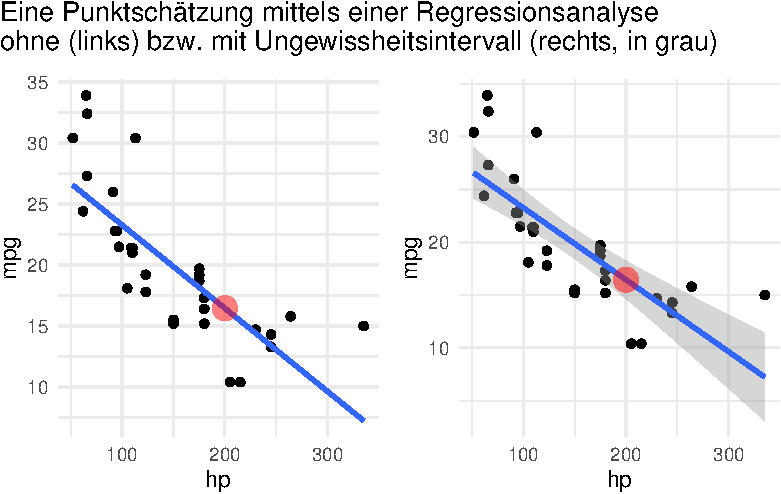
\includegraphics{./Inferenz_files/figure-pdf/fig-punktschaetzer2-1.pdf}

}

\caption{\label{fig-punktschaetzer2}Eine Punktschätzung und ihre
Ungewissheit}

\end{figure}

In Abb. Abbildung~\ref{fig-punktschaetzer2}, rechts, ist die
Ungewissheit in den Regressionskoeffizienten visualisiert: Wie sicher
sind wir uns zur Stärke des Zusammenhangs von X und Y?

Auch wenn wir uns \emph{sicher} im Hinblick auf die Regressionsgewichte
in Abb. Abbildung~\ref{fig-ungewiss2} \emph{bliebe eine
Restungewissheit}: Unsere Schätzungen wären auch dann nicht sicher,
nicht fehlerfrei. Das liegt daran, da das Modell nicht alle Einflüsse
auf Y berücksichtigt, sondern nur einen, hier als X bezeichnet.

In Abb. Abbildung~\ref{fig-ungewiss2} ist nicht nur die Ungewissheit
durch die Regressionsgewichte, sondern auch die ``Restungewissheit''
dargestellt. In diesem Fall spricht man von einem
``Vorhersageintervall'', da man nicht nur von ``typischen Fällen'' auf
der Regressiongeraden spricht, sondern für echte Fälle Vorhersagen
(Schätzungen) tätigt, wo auch die zweite Art von Ungewissheit relevant
ist.

\begin{figure}

{\centering 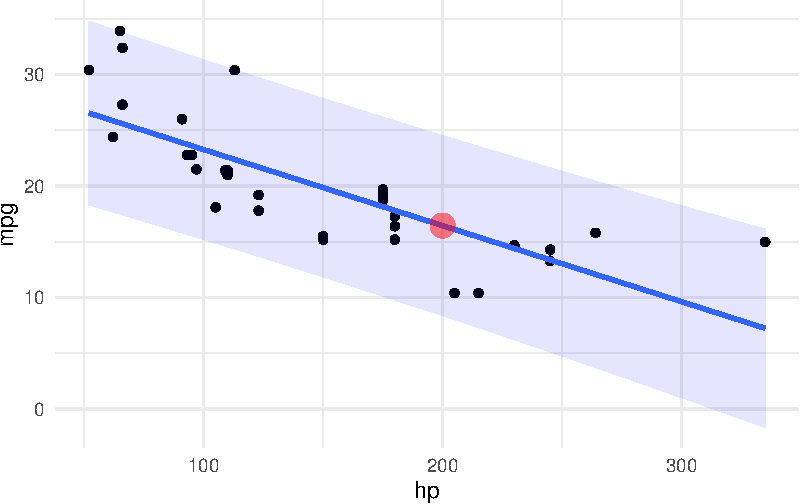
\includegraphics{./Inferenz_files/figure-pdf/fig-ungewiss2-1.pdf}

}

\caption{\label{fig-ungewiss2}Zweifache Ungewissheit in den
Regressionskoeffizienten - Vorhersageintervall}

\end{figure}

Wie man sieht, wird die Ungewissheit \emph{größer}, wenn man beide Arten
der Ungewissheit berücksichtigt. Das Vorhersage-Intervall berücksichtigt
Ungewissheit in \(\beta_0, \beta_1, \epsilon\) bei der Vorhersage von
\(\hat{y_i}\).

🏋 Geben Sie ein vergleichbares Beispiel an!

\hypertarget{konfidenzintervall}{%
\subsection{Konfidenzintervall}\label{konfidenzintervall}}

Wir sehen hier, dass ein ``Ungewissheitskorridor'' angegeben wird.
Entsprechend wird nicht ein \emph{Punktschätzer}, sondern ein
\emph{Schätzbereich} angegeben. Man spricht auch von einem
\emph{Konfidenzintervall} oder \emph{Unsicherheitsbereich}\footnote{Tatsächlich
  gibt es mehrere Synonyme oder ähnliche Begriffe für
  Konfidenzintervall. Wir kommen später darauf detaillierter zu
  sprechen.}

Ein Konfidenzintervall wird häufig mit 90\% oder 95\% Genauigkeit
angegeben. Im Kontext der Bayes-Analyse ist das einfach zu
interpretieren. Sagen wir, wir finden, dass in einem Modell ein
95\%-Konfidenzintervall für den Anteil der R-Fans angegeben wird, dass
sich von 40 bis 44 Prozent erstreckt. Dieser Befund läßt sich so
interpretieren: ``Laut Modell liegt der gesuchte Anteil mit einer
Wahrscheinlichkeit von 95\% im Bereich von 44 bis 44 Prozentpunkten.''

\begin{tcolorbox}[enhanced jigsaw, colframe=quarto-callout-important-color-frame, breakable, titlerule=0mm, left=2mm, colbacktitle=quarto-callout-important-color!10!white, opacityback=0, colback=white, opacitybacktitle=0.6, toptitle=1mm, rightrule=.15mm, toprule=.15mm, bottomrule=.15mm, bottomtitle=1mm, title=\textcolor{quarto-callout-important-color}{\faExclamation}\hspace{0.5em}{Wichtig}, leftrule=.75mm, arc=.35mm, coltitle=black]

Ein Konfidenzintervall gibt einen Schätzbereich plausibler Werte für den
gesuchten Wert in der Population (den Parameter) an.

\end{tcolorbox}

🏋 Interpretieren Sie den Ungewissheitskorridor!

\hypertarget{klassische-vs.-bayes-inferenz}{%
\section{Klassische
vs.~Bayes-Inferenz}\label{klassische-vs.-bayes-inferenz}}

\hypertarget{klassische-inferenz-frequentismus}{%
\subsection{Klassische Inferenz:
Frequentismus}\label{klassische-inferenz-frequentismus}}

\begin{itemize}
\tightlist
\item
  Die Berücksichtigung von Vorwissen zum Sachgegenstand wird vom
  Frequentismus als subjektiv zurückgewiesen.
\item
  Nur die Daten selber fliesen in die Ergebnisse ein
\item
  Wahrscheinlichkeit wird über relative Häufigkeiten definiert.
\item
  Es ist nicht möglich, die Wahrscheinlichkeit einer Hypothese
  anzugeben.
\item
  Stattdessen wird angegeben, wie häufig eine vergleichbare Datenlage zu
  erwarten ist, wenn die Hypothese gilt und der Versuch sehr häufig
  wiederholt ist.
\item
  Ein Großteil der Forschung (in den Sozialwissenschaften) verwendet
  diesen Ansatz.
\end{itemize}

\hypertarget{bayesianische-inferenz}{%
\subsection{Bayesianische Inferenz}\label{bayesianische-inferenz}}

\begin{itemize}
\tightlist
\item
  Vorwissen (Priori-Wissen) fließt explizit in die Analyse ein (zusammen
  mit den Daten).
\item
  \emph{Wenn} das Vorwissen gut ist, wird die Vorhersage genauer,
  ansonsten ungenauer.
\item
  Die Wahl des Vorwissens muss explizit (kritisierbar) sein.
\item
  In der Bayes-Inferenz sind Wahrscheinlichkeitsaussagen für Hypothesen
  möglich.
\item
  Die Bayes-Inferenz erfordert mitunter viel Rechenzeit und ist daher
  erst in den letzten Jahren (für gängige Computer) komfortabel
  geworden.
\end{itemize}

\hypertarget{vergleich-von-wahrscheinlichkeitsaussagen}{%
\subsection{Vergleich von
Wahrscheinlichkeitsaussagen}\label{vergleich-von-wahrscheinlichkeitsaussagen}}

\hypertarget{frequentismus}{%
\subsubsection{Frequentismus}\label{frequentismus}}

Die zentrale Statistik heißt der \emph{p-Wert}

Der p-Wert ist so definiert: ``Wie wahrscheinlich ist der Wert der
Teststatistik (oder noch extremere Werte), vorausgesetzt die
Nullhypothese gilt und man wiederholt den Versuch unendlich oft (mit
gleichen Bedingungen, aber zufällig verschieden und auf Basis unseres
Modells)?''

Findet man \(p<.05\) (oder einen anderen Prozentwert, aber meistens wird
5\% hergenommen), so spricht man von ``(statistischer) Signifikanz'' und
nimmt dies als Beleg, dass man einen Effekt gefunden hat, die Hypothese
eines Nulleffekts (z.B. kein Zusammenhang von X und Y) also verwerfen
kann.

\hypertarget{bayes-statistik}{%
\subsubsection{Bayes-Statistik}\label{bayes-statistik}}

Die zentrale Statistik ist die \emph{Posteriori-Verteilung}.

Die Posteriori-Verteilung beantwortet uns die Frage: ``Wie
wahrscheinlich ist die Forschungshypothese, jetzt, nachdem wir die Daten
kennen, auf Basis unseres Modells?''

🏋 Recherchieren Sie eine Definition des p-Werts und lesen Sie sie genau.

\href{https://data-se.netlify.app/2022/01/27/warum-bayes/}{In diesem
Post} wird für Bayes geworben und (vielleicht einseitig) Stellung pro
Bayes bezogen.

\hypertarget{frequentist-und-bayesianer}{%
\subsection{Frequentist und
Bayesianer}\label{frequentist-und-bayesianer}}

Im Cartoon 1132 \href{https://xkcd.com/}{von xkcd} wird sich über das
Nicht-Berücksichtigen von Vorab-Informationen (Prior-Verteilung) lustig
gemacht, s. Abbildung~\ref{fig-xkcd-bayes}.

\begin{figure}

{\centering 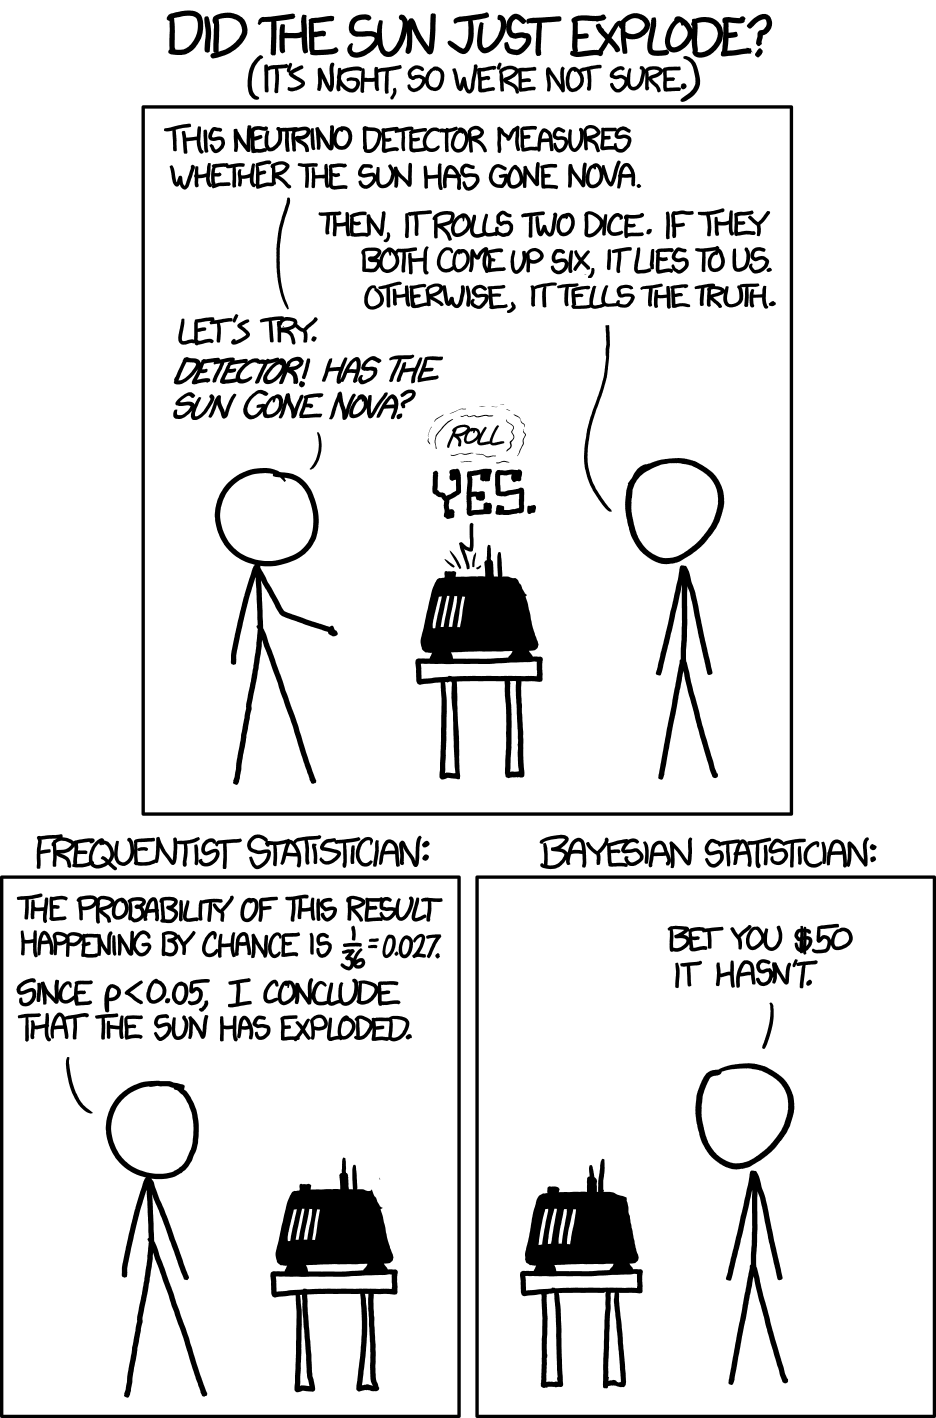
\includegraphics[width=0.5\textwidth,height=\textheight]{./img/frequentists_vs_bayesians_2x.png}

}

\caption{\label{fig-xkcd-bayes}Frequentist wettet mit Bayesianer}

\end{figure}

\href{https://xkcd.com/1132/}{Quelle}

\hypertarget{der-p-wert-ist-wenig-intuitiv}{%
\subsection{Der p-Wert ist wenig
intuitiv}\label{der-p-wert-ist-wenig-intuitiv}}

from Imgflip Meme Generator

\hypertarget{beispiel-zum-nutzen-von-apriori-wissen-1}{%
\subsection{Beispiel zum Nutzen von Apriori-Wissen
1}\label{beispiel-zum-nutzen-von-apriori-wissen-1}}

Ein Betrunkener behauptet, er könne hellsehen. Er wirft eine Münze 10
Mal und sagt jedes Mal korrekt vorher, welche Seite oben landen wird.

Die Wahrscheinlichkeit dieses Ergebnisses ist sehr gering (\(2^{-10}\))
unter der Hypothese, dass die Münze fair ist, dass Ergebnis also
``zufällig'' ist.

Unser Vorwissen lässt uns allerdings trotzdem an der Hellsichtigkeit des
Betrunkenen zweifeln, so dass die meisten von uns die Hypothese von der
Zufälligkeit des Ergebnisses wohl nicht verwerfen.

\hypertarget{beispiel-zum-nutzen-von-apriori-wissen-2}{%
\subsection{Beispiel zum Nutzen von Apriori-Wissen
2}\label{beispiel-zum-nutzen-von-apriori-wissen-2}}

Eine Studie (vgl. Gelman, Hill, und Vehtari (2021)) fand einen ``großen
Effekt'' auf das Einkommen von Babies, eine Stunde pro Woche während
zwei Jahren an einem psychosozialen Entwicklungsprogramm teilnahmen (im
Vergleich zu einer Kontrollgruppe), \(n=127\).

Nach 20 Jahren war das mittlere Einkommen der Experimentalgruppe um 42\%
höher (als in der Kontrollgruppe) mit einem Konfidenzintervall von
{[}+2\%,+98\%{]}.

Allerdings lässt uns unser Vorwissen vermuten, dass so ein Treatment das
Einkommen nach 20 Jahren kaum verdoppeln lässt. Wir würden den Effekt
lieber in einem konservativeren Intervall schätzen (enger um Null).

\hypertarget{literatur-1}{%
\section{Literatur}\label{literatur-1}}

Bei Gelman, Hill, und Vehtari (2021), Kap. 1 findet sich eine
Darstellung ähnlich zu der in diesem Kapitel.

\hypertarget{aufgaben}{%
\section{Aufgaben}\label{aufgaben}}

\begin{enumerate}
\def\labelenumi{\arabic{enumi}.}
\tightlist
\item
  \href{https://datenwerk.netlify.app/posts/griech-buchstaben-inferenz/griech-buchstaben-inferenz/}{Griech-Buchstaben-Inferenz}
\item
  \href{https://datenwerk.netlify.app/posts/korr-als-regr/korr-als-regr/}{korr-als-regr}
\item
  \href{https://datenwerk.netlify.app/posts/ttest-als-regr/ttest-als-regr/}{ttest-als-regr}
\item
  \href{https://datenwerk.netlify.app/posts/ttest-skalenniveau/ttest-skalenniveau/}{ttest-skalenniveau}
\item
  \href{https://datenwerk.netlify.app/posts/adjustieren2/adjustieren2/}{adjustieren2}
\item
  \href{https://datenwerk.netlify.app/posts/inferenz-fuer-alle/inferenz-fuer-alle}{inferenz-fuer-alle}
\item
  \href{https://datenwerk.netlify.app/posts/adjustieren1/adjustieren1.html}{adjustieren1}
\item
  \href{https://datenwerk.netlify.app/posts/ungewiss-arten-regr/ungewiss-arten-regr.html}{ungewiss-arten-regr}
\item
  \href{https://datenwerk.netlify.app/posts/vorhersageintervall1/vorhersageintervall1.html}{vorhersageintervall1}
\item
  \href{https://datenwerk.netlify.app/posts/lm-standardfehler/lm-standardfehler}{lm-standardfehler}
\item
  \href{https://datenwerk.netlify.app/posts/punktschaetzer-reicht-nicht/punktschaetzer-reicht-nicht.html}{punktschaetzer-reicht-nicht}
\end{enumerate}

\hypertarget{section-1}{%
\section{---}\label{section-1}}

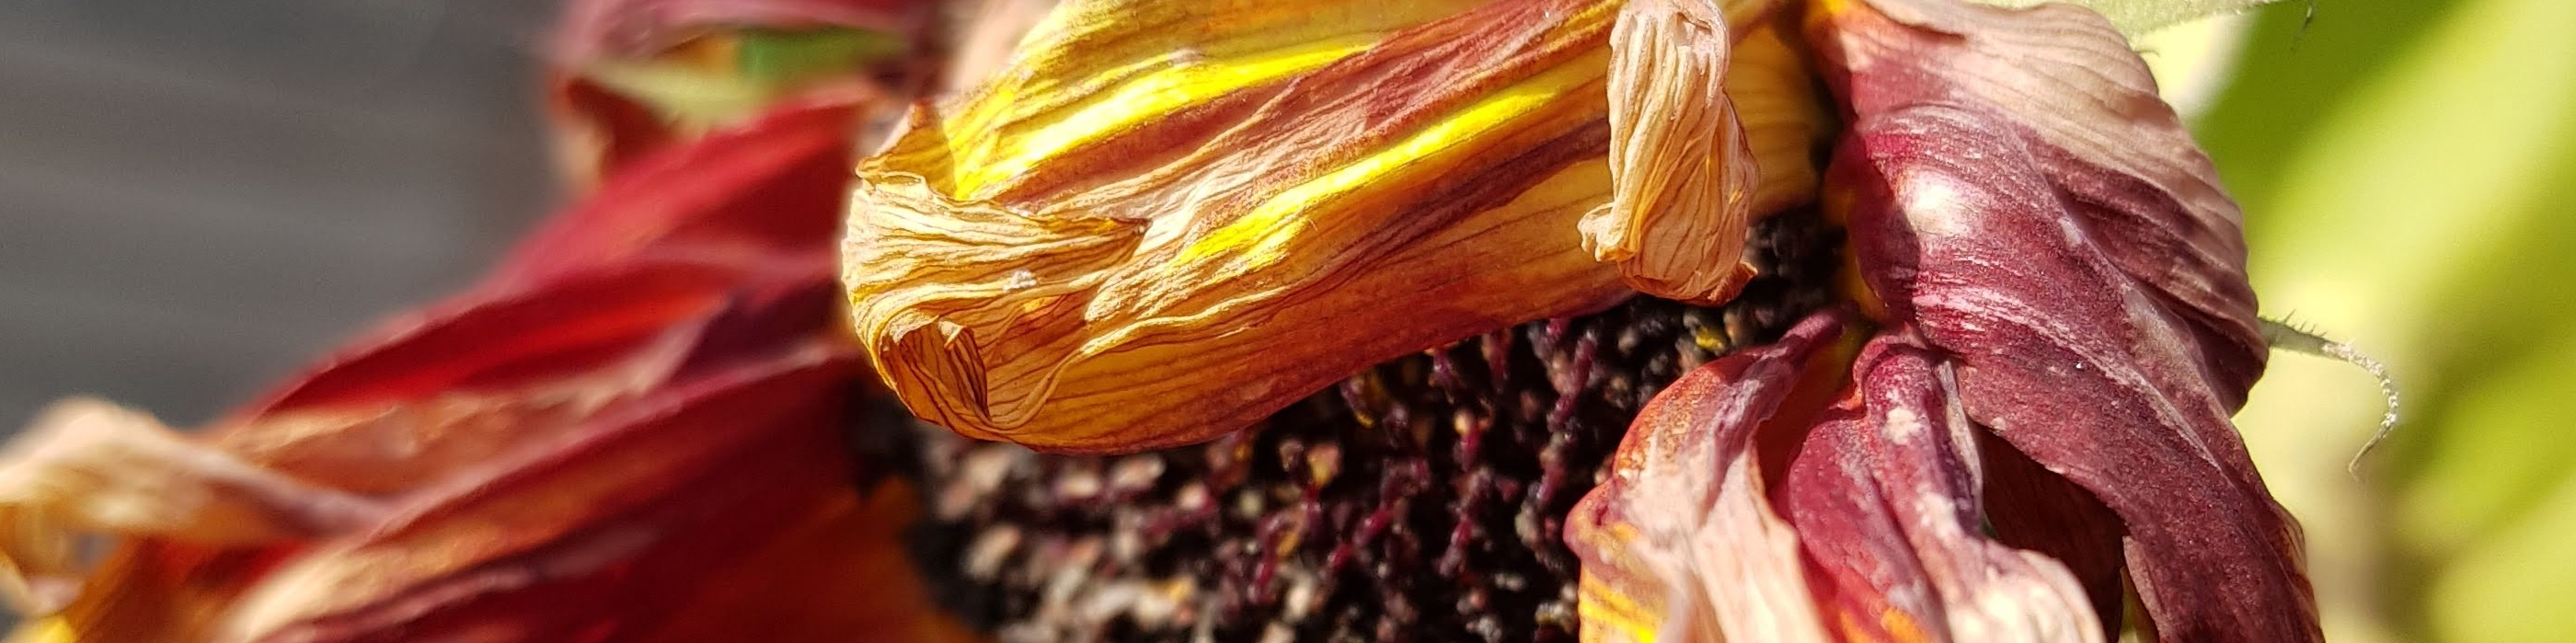
\includegraphics[width=1\textwidth,height=\textheight]{./img/outro-02.jpg}

\bookmarksetup{startatroot}

\hypertarget{wahrscheinlichkeit}{%
\chapter{Wahrscheinlichkeit}\label{wahrscheinlichkeit}}

\hypertarget{lernsteuerung-1}{%
\section{Lernsteuerung}\label{lernsteuerung-1}}

\hypertarget{lernziele-2}{%
\subsection{Lernziele}\label{lernziele-2}}

Nach Absolvieren des jeweiligen Kapitels sollen folgende Lernziele
erreicht sein.

Sie können \ldots{}

\begin{itemize}
\tightlist
\item
  die Grundbegriffe der Wahrscheinlichkeitsrechnung erläuternd
  definieren
\item
  die drei Arten der direkten Ermittlung von Wahrscheinlichkeit
  erläutern
\item
  typische Relationen (Operationen) von Ereignissen anhand von
  Beispielen veranschaulichen
\item
  mit Wahrscheinlichkeiten rechnen
\end{itemize}

\hypertarget{pruxfcfungsrelevanter-stoff}{%
\subsection{Prüfungsrelevanter
Stoff}\label{pruxfcfungsrelevanter-stoff}}

Lesen Sie dazu Bourier (2018), Kap. 2-4. Weitere Übungsaufgaben finden
Sie im dazugehörigen Übungsbuch, Bourier (2022).

\hypertarget{zentrale-begriffe}{%
\subsection{Zentrale Begriffe}\label{zentrale-begriffe}}

\hypertarget{grundbegriffe}{%
\subsubsection{Grundbegriffe}\label{grundbegriffe}}

\begin{itemize}
\tightlist
\item
  Zufallsvorgang (Zufallsexperiment)
\item
  Elementarereignis
\item
  Ereignisraum
\item
  Zufallsereignis (zufälliges Ereignis)
\item
  Sicheres Ereignis
\item
  Unmögliches Ereignis
\end{itemize}

\hypertarget{wahrscheinlichkeitsbegriffe}{%
\subsubsection{Wahrscheinlichkeitsbegriffe}\label{wahrscheinlichkeitsbegriffe}}

\begin{itemize}
\tightlist
\item
  Klassische Wahrscheinlichkeit (LaPlace'sche Wahrscheinlichkeit)
\item
  Statistische (empirische) Wahrscheinlichkeitsermittlung
\item
  Subjektive (Bayes) Wahrscheinlichkeitsermittlung
\end{itemize}

\hypertarget{wahrscheinlichkeitsrelationen}{%
\subsubsection{Wahrscheinlichkeitsrelationen}\label{wahrscheinlichkeitsrelationen}}

\begin{itemize}
\tightlist
\item
  Vereinigung von Ereignissen
\item
  Schnitt(menge) von Ereignissen
\item
  Komplementärereignis
\item
  Vollständiges Ereignissystem
\item
  Kolmogorovs Definition von Wahrscheinlichkeit
\end{itemize}

\hypertarget{wahrscheinlichkeitsrechnung}{%
\subsubsection{Wahrscheinlichkeitsrechnung}\label{wahrscheinlichkeitsrechnung}}

\begin{itemize}
\tightlist
\item
  Allgemeiner Additionsssatz
\item
  Disjunkte Ereignisse
\item
  Additionssatz für disjunkte Ereignisse
\item
  Bedingte Wahrscheinlichkeit
\item
  (Stochastische) Unabhängigkeit
\item
  Baumdiagramm für gemeinsame Wahrscheinlichkeit
\item
  Allgemeiner Multiplikationssatz
\item
  Multiplikationssatz für unabhängige Ereignisse
\item
  Totale Wahrscheinlichkeit
\item
  Satz von Bayes
\end{itemize}

\hypertarget{begleitvideos-1}{%
\subsection{Begleitvideos}\label{begleitvideos-1}}

\begin{itemize}
\tightlist
\item
  \href{https://youtu.be/rR6NspapEyo}{Video zum Thema
  Wahrscheinlichkeit}
\end{itemize}

\hypertarget{unterstuxfctzung-wahrscheinlichkeit-in-bildern}{%
\section{Unterstützung: Wahrscheinlichkeit in
Bildern}\label{unterstuxfctzung-wahrscheinlichkeit-in-bildern}}

Wahrscheinlichkeit in Bildern: zur einfachen Erschließung des Materials,
ein Unterstützungsangebot.

Im Folgenden sind einige Schlüsselbegriffe und -regeln in
(ver-)einfach(t)er Form schematisch bzw. visuell dargestellt mit dem
Ziel, den Stoff einfacher zu erschließen.

\hypertarget{zufall}{%
\subsection{Zufall}\label{zufall}}

Werfen Sie eine Münze!

Diese hier zum Beispiel:

\begin{figure}

{\centering 
\includegraphics[width=0.1\textwidth,height=\textheight]{./img/1024px-Coin-155597.svg.png}

}

\end{figure}

\href{https://pixabay.com/pt/moeda-euro-europa-fran\%C3\%A7a-dinheiro-155597}{Quelle:
By OpenClipartVectors, CC0}

Wiederholen Sie den Versuch 10, nein, 100, nein 1000, nein: \(10^6\)
Mal.

Notieren Sie das Ergebnis!

Oder probieren Sie die
\href{https://seeing-theory.brown.edu/basic-probability/index.html\#section1}{App
der Brown University}.

\hypertarget{relationen-von-mengen}{%
\subsection{Relationen von Mengen}\label{relationen-von-mengen}}

Venn-Diagramme eigenen sich, um typische Operationen (Relationen) auf
Mengen zu visualisieren.

\hypertarget{uxfcberblick}{%
\subsubsection{Überblick}\label{uxfcberblick}}

Die folgenden Diagramme stammen von
\href{https://en.wikipedia.org/wiki/Venn_diagram}{Wikipedia (En)}.

Wir gehen von Ereignisraum \(\Omega\) aus, mit dem Ereignis \(A\) als
Teilmenge: \(A \subset B\).

\begin{figure}

\begin{minipage}[t]{0.50\linewidth}

{\centering 

\raisebox{-\height}{

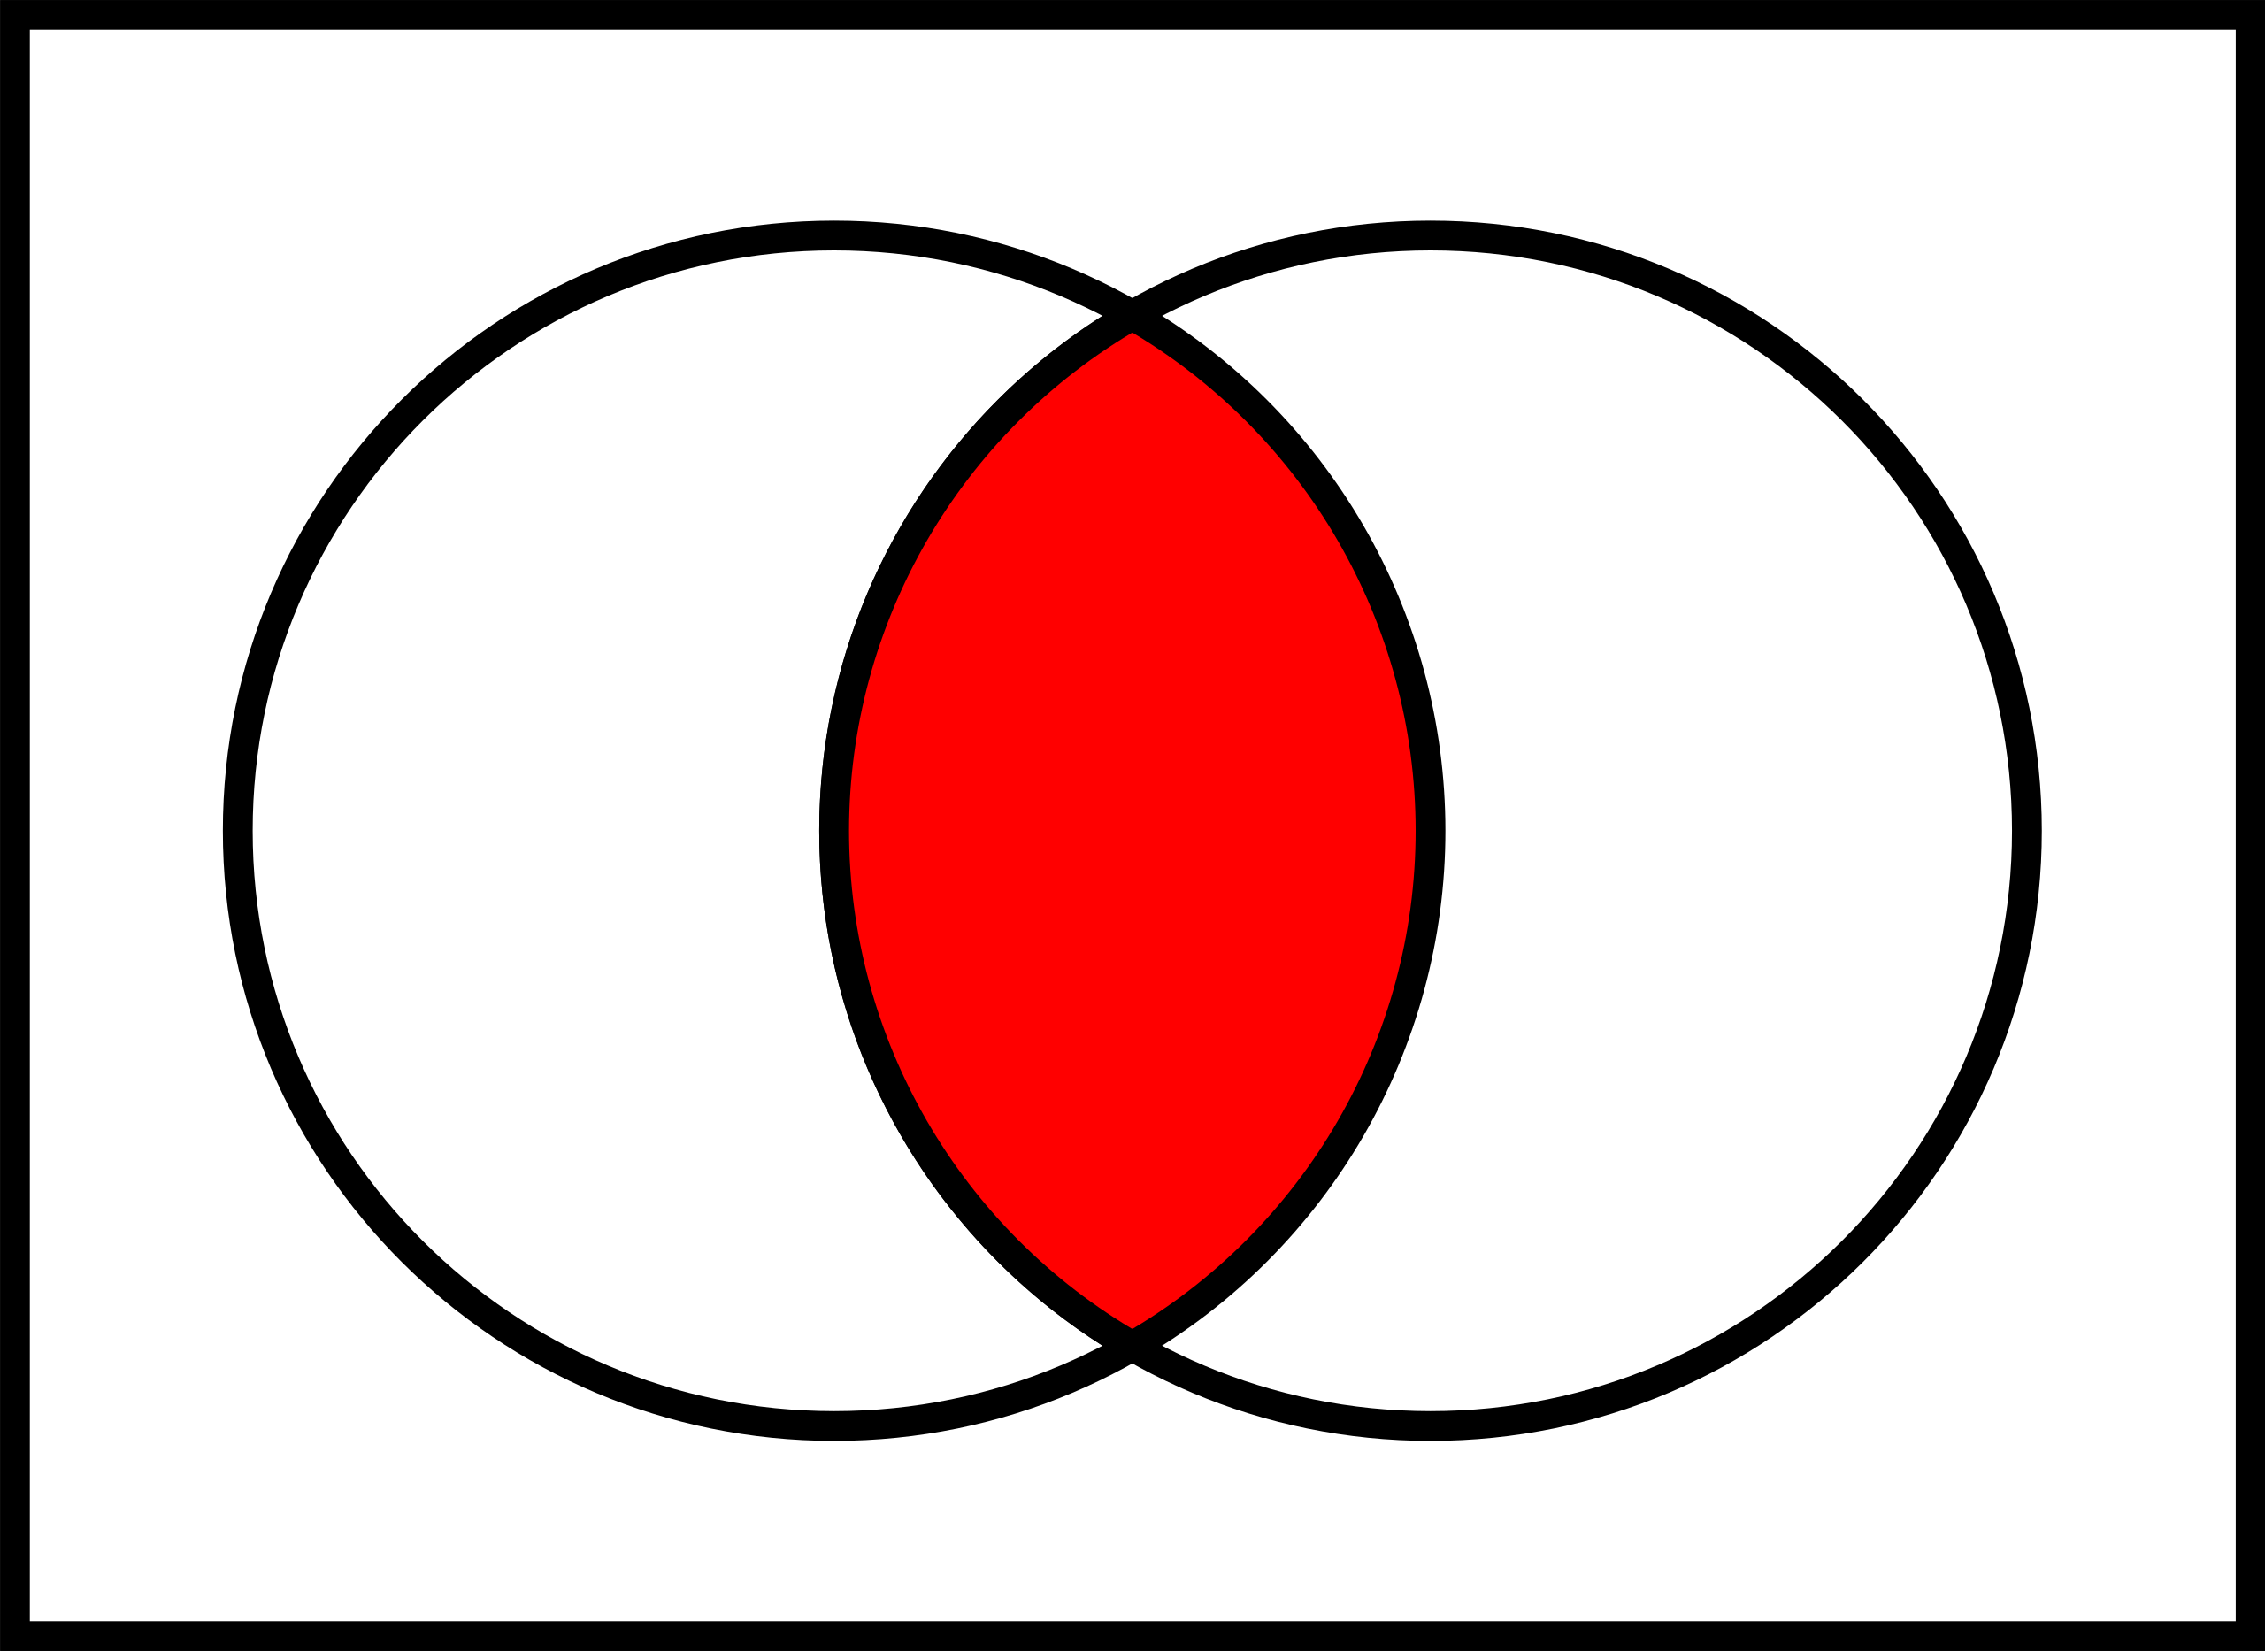
\includegraphics{./img/Venn0001.svg.png}

}

\caption{\(A \cap B\)}

}

\end{minipage}%
%
\begin{minipage}[t]{0.50\linewidth}

{\centering 

\raisebox{-\height}{

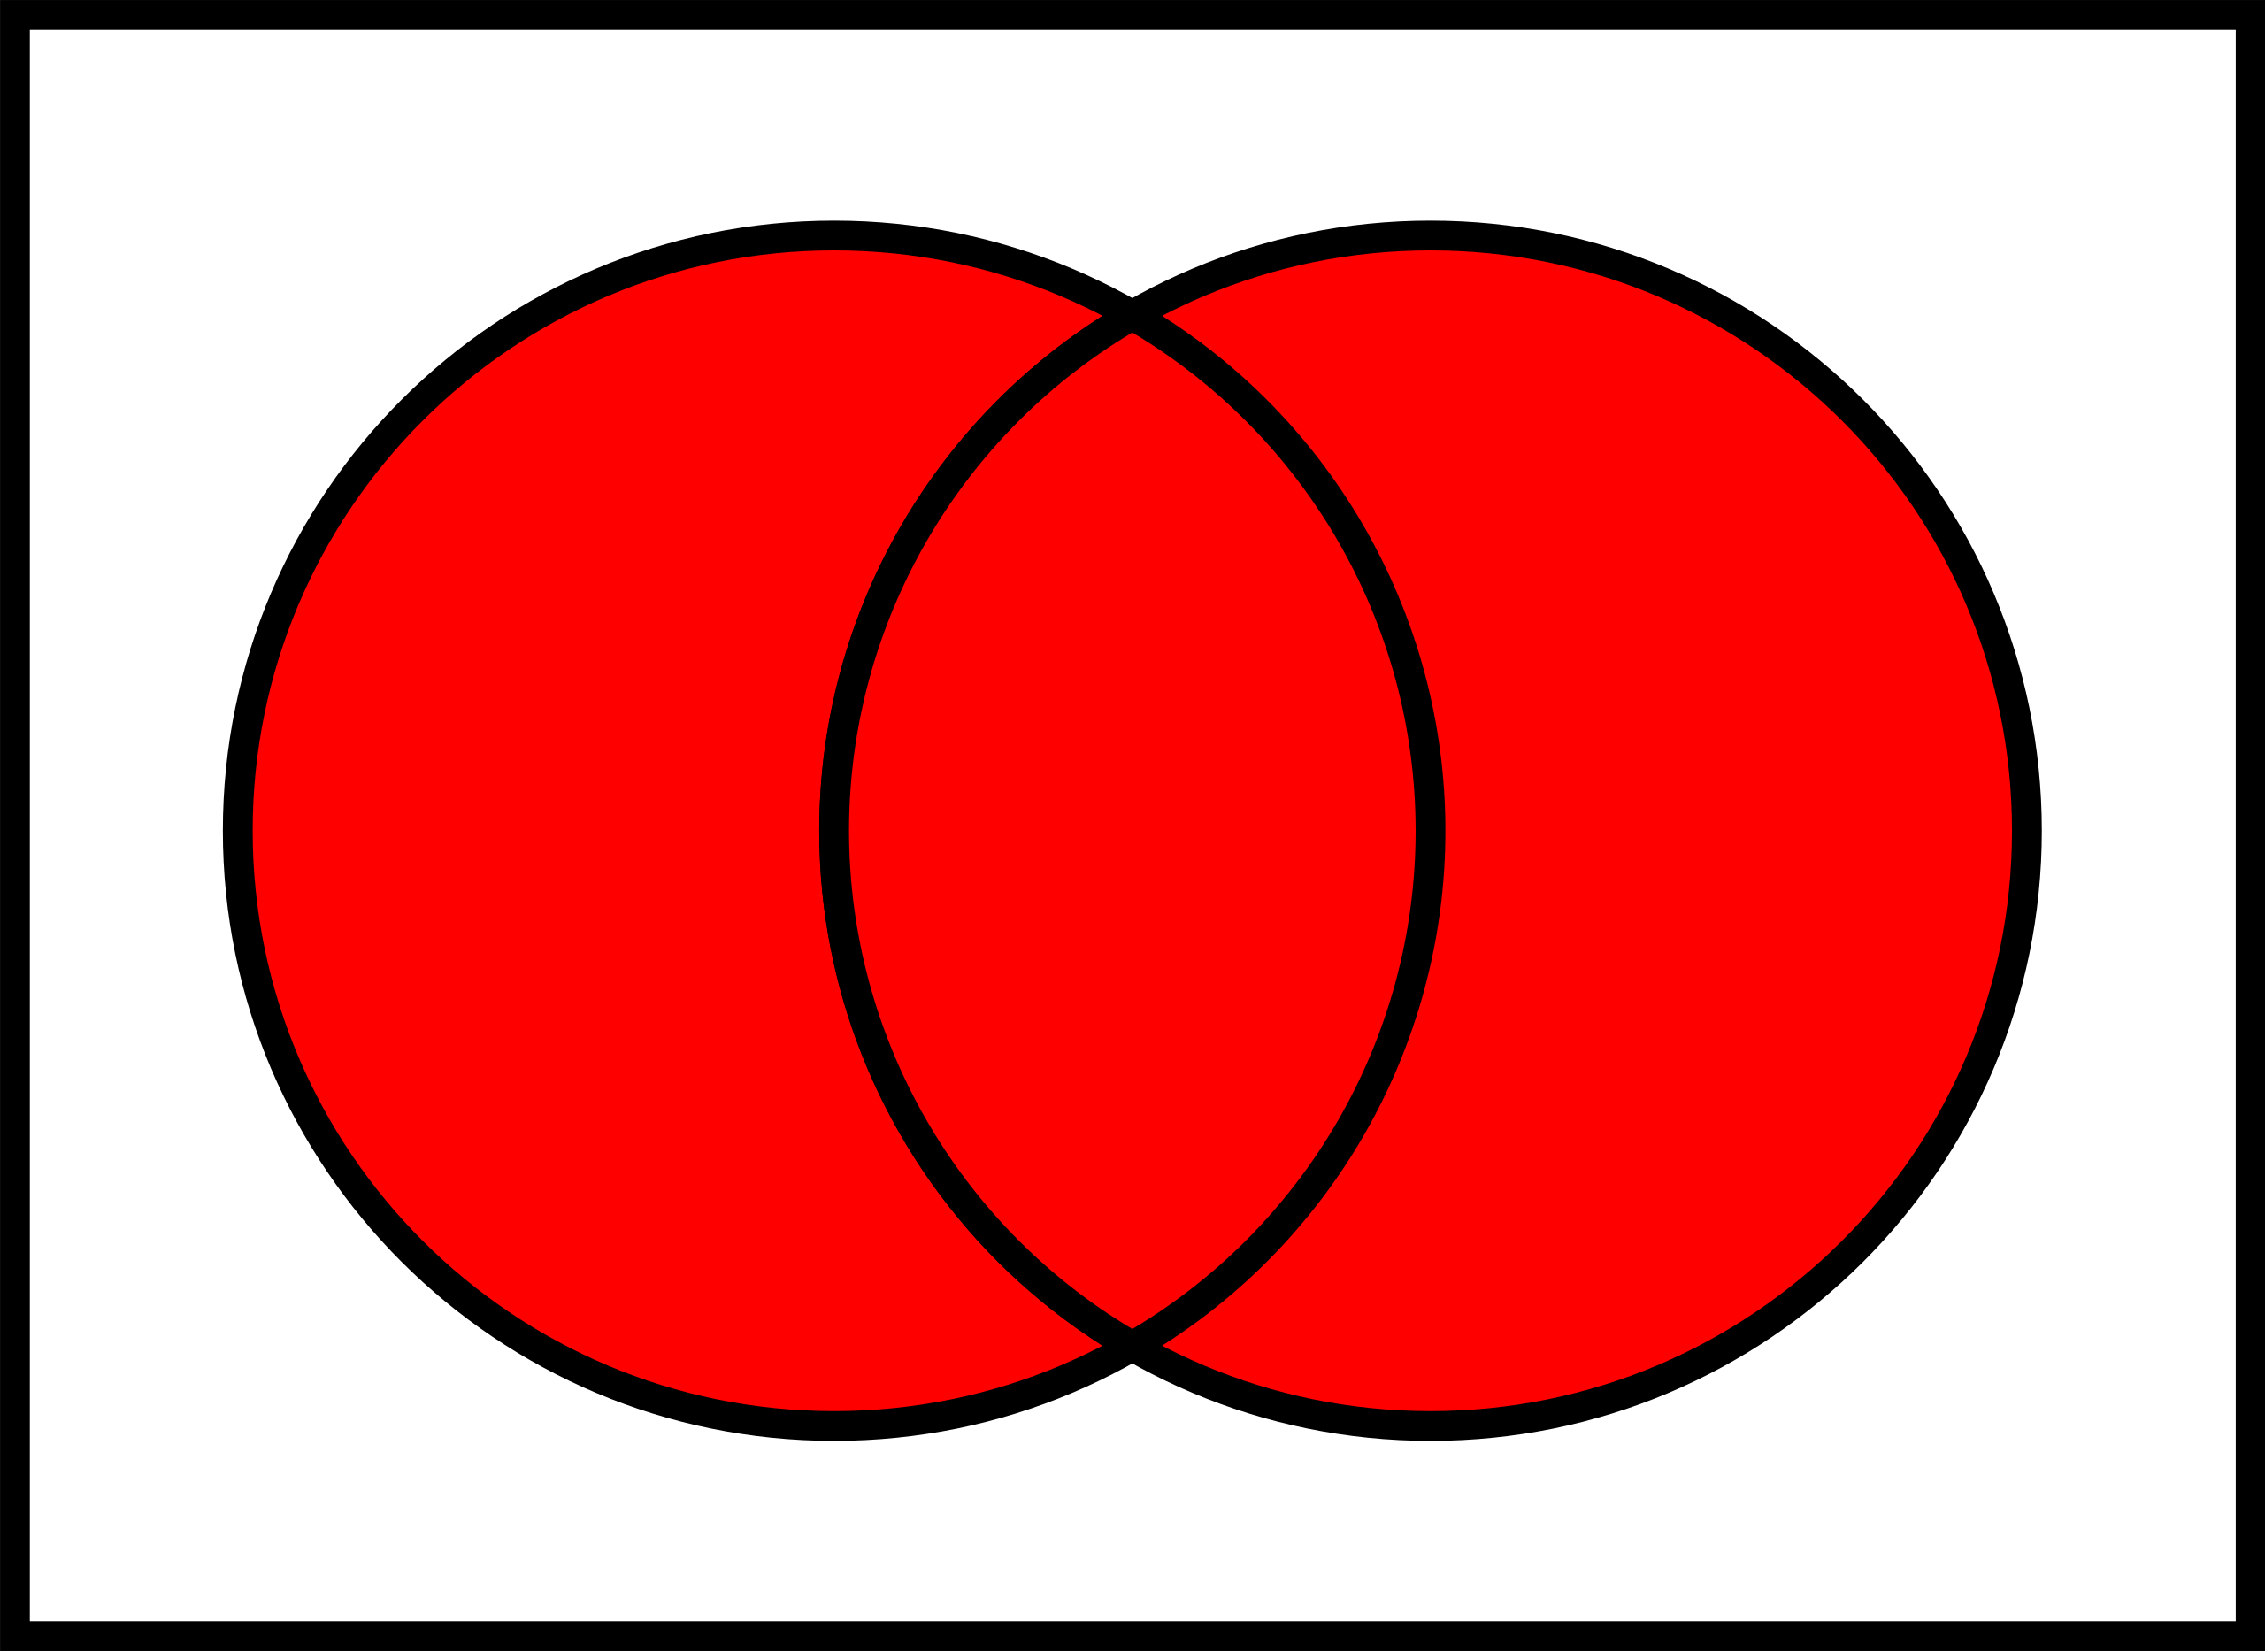
\includegraphics{./img/Venn0111.svg.png}

}

\caption{\(A \cup B\)}

}

\end{minipage}%
\newline
\begin{minipage}[t]{0.50\linewidth}

{\centering 

\raisebox{-\height}{

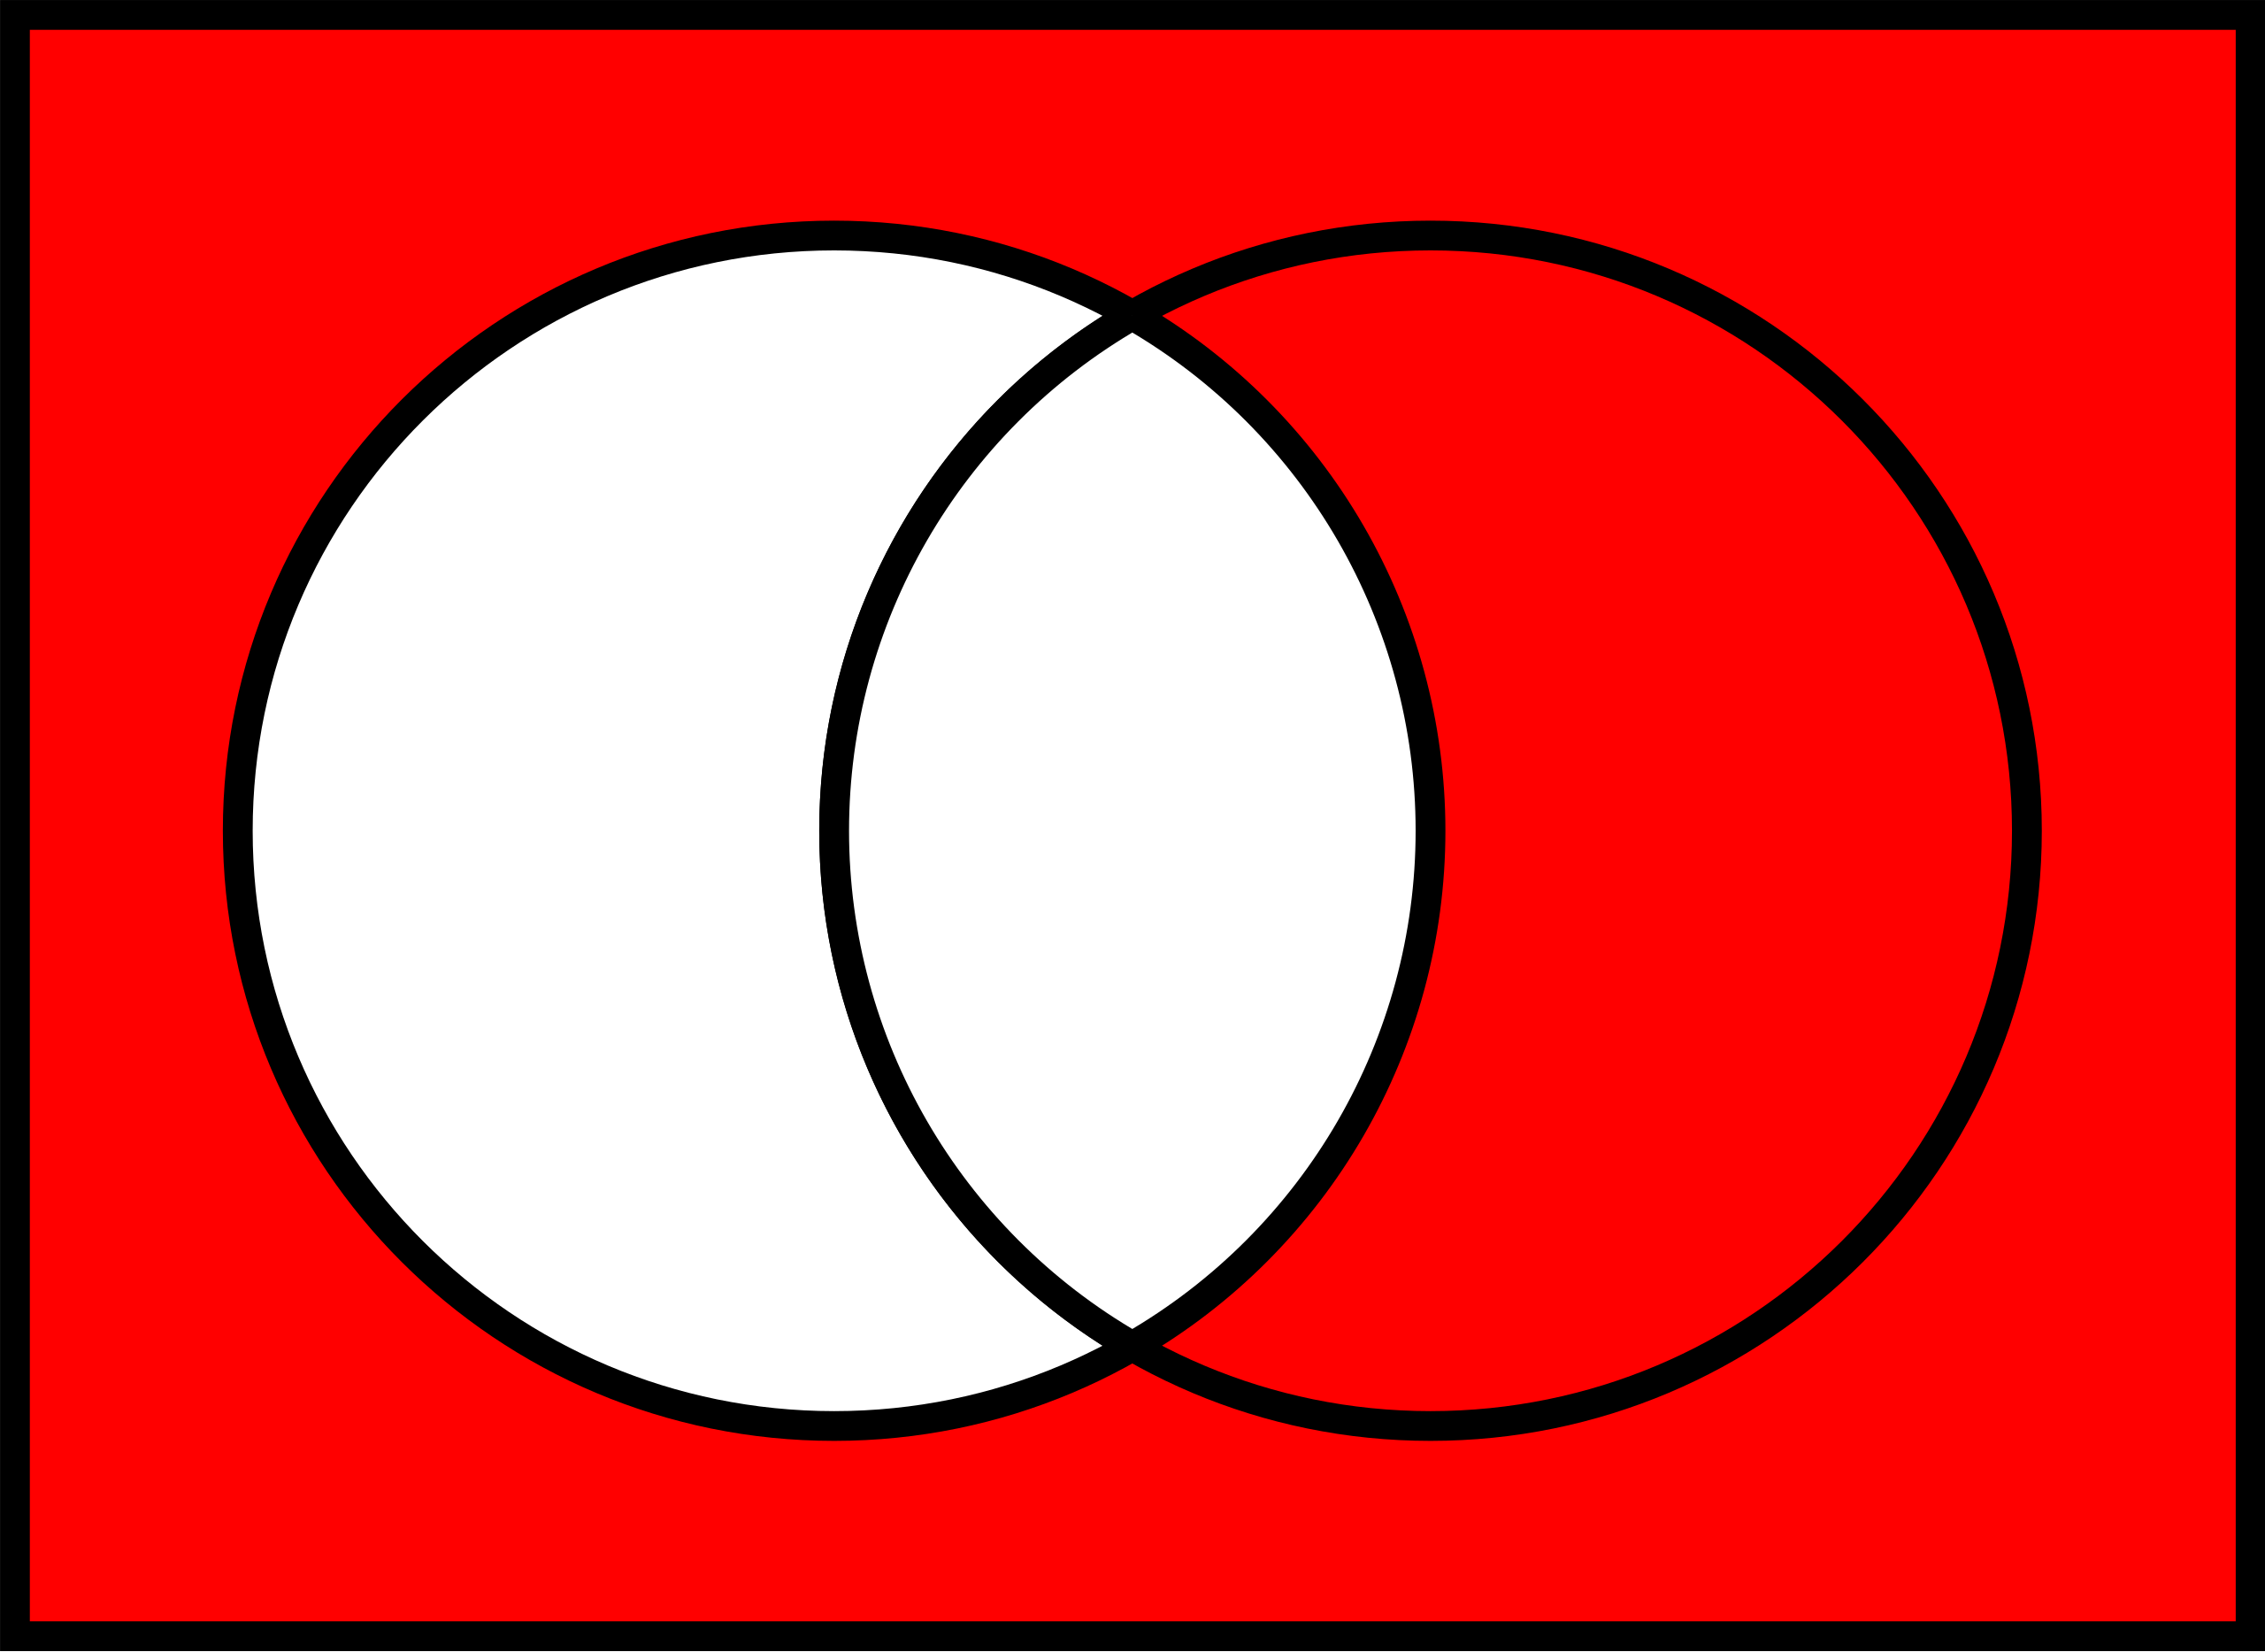
\includegraphics{./img/2560px-Venn1010.svg.png}

}

\caption{\(\bar{A}\)}

}

\end{minipage}%
%
\begin{minipage}[t]{0.50\linewidth}

{\centering 

\raisebox{-\height}{

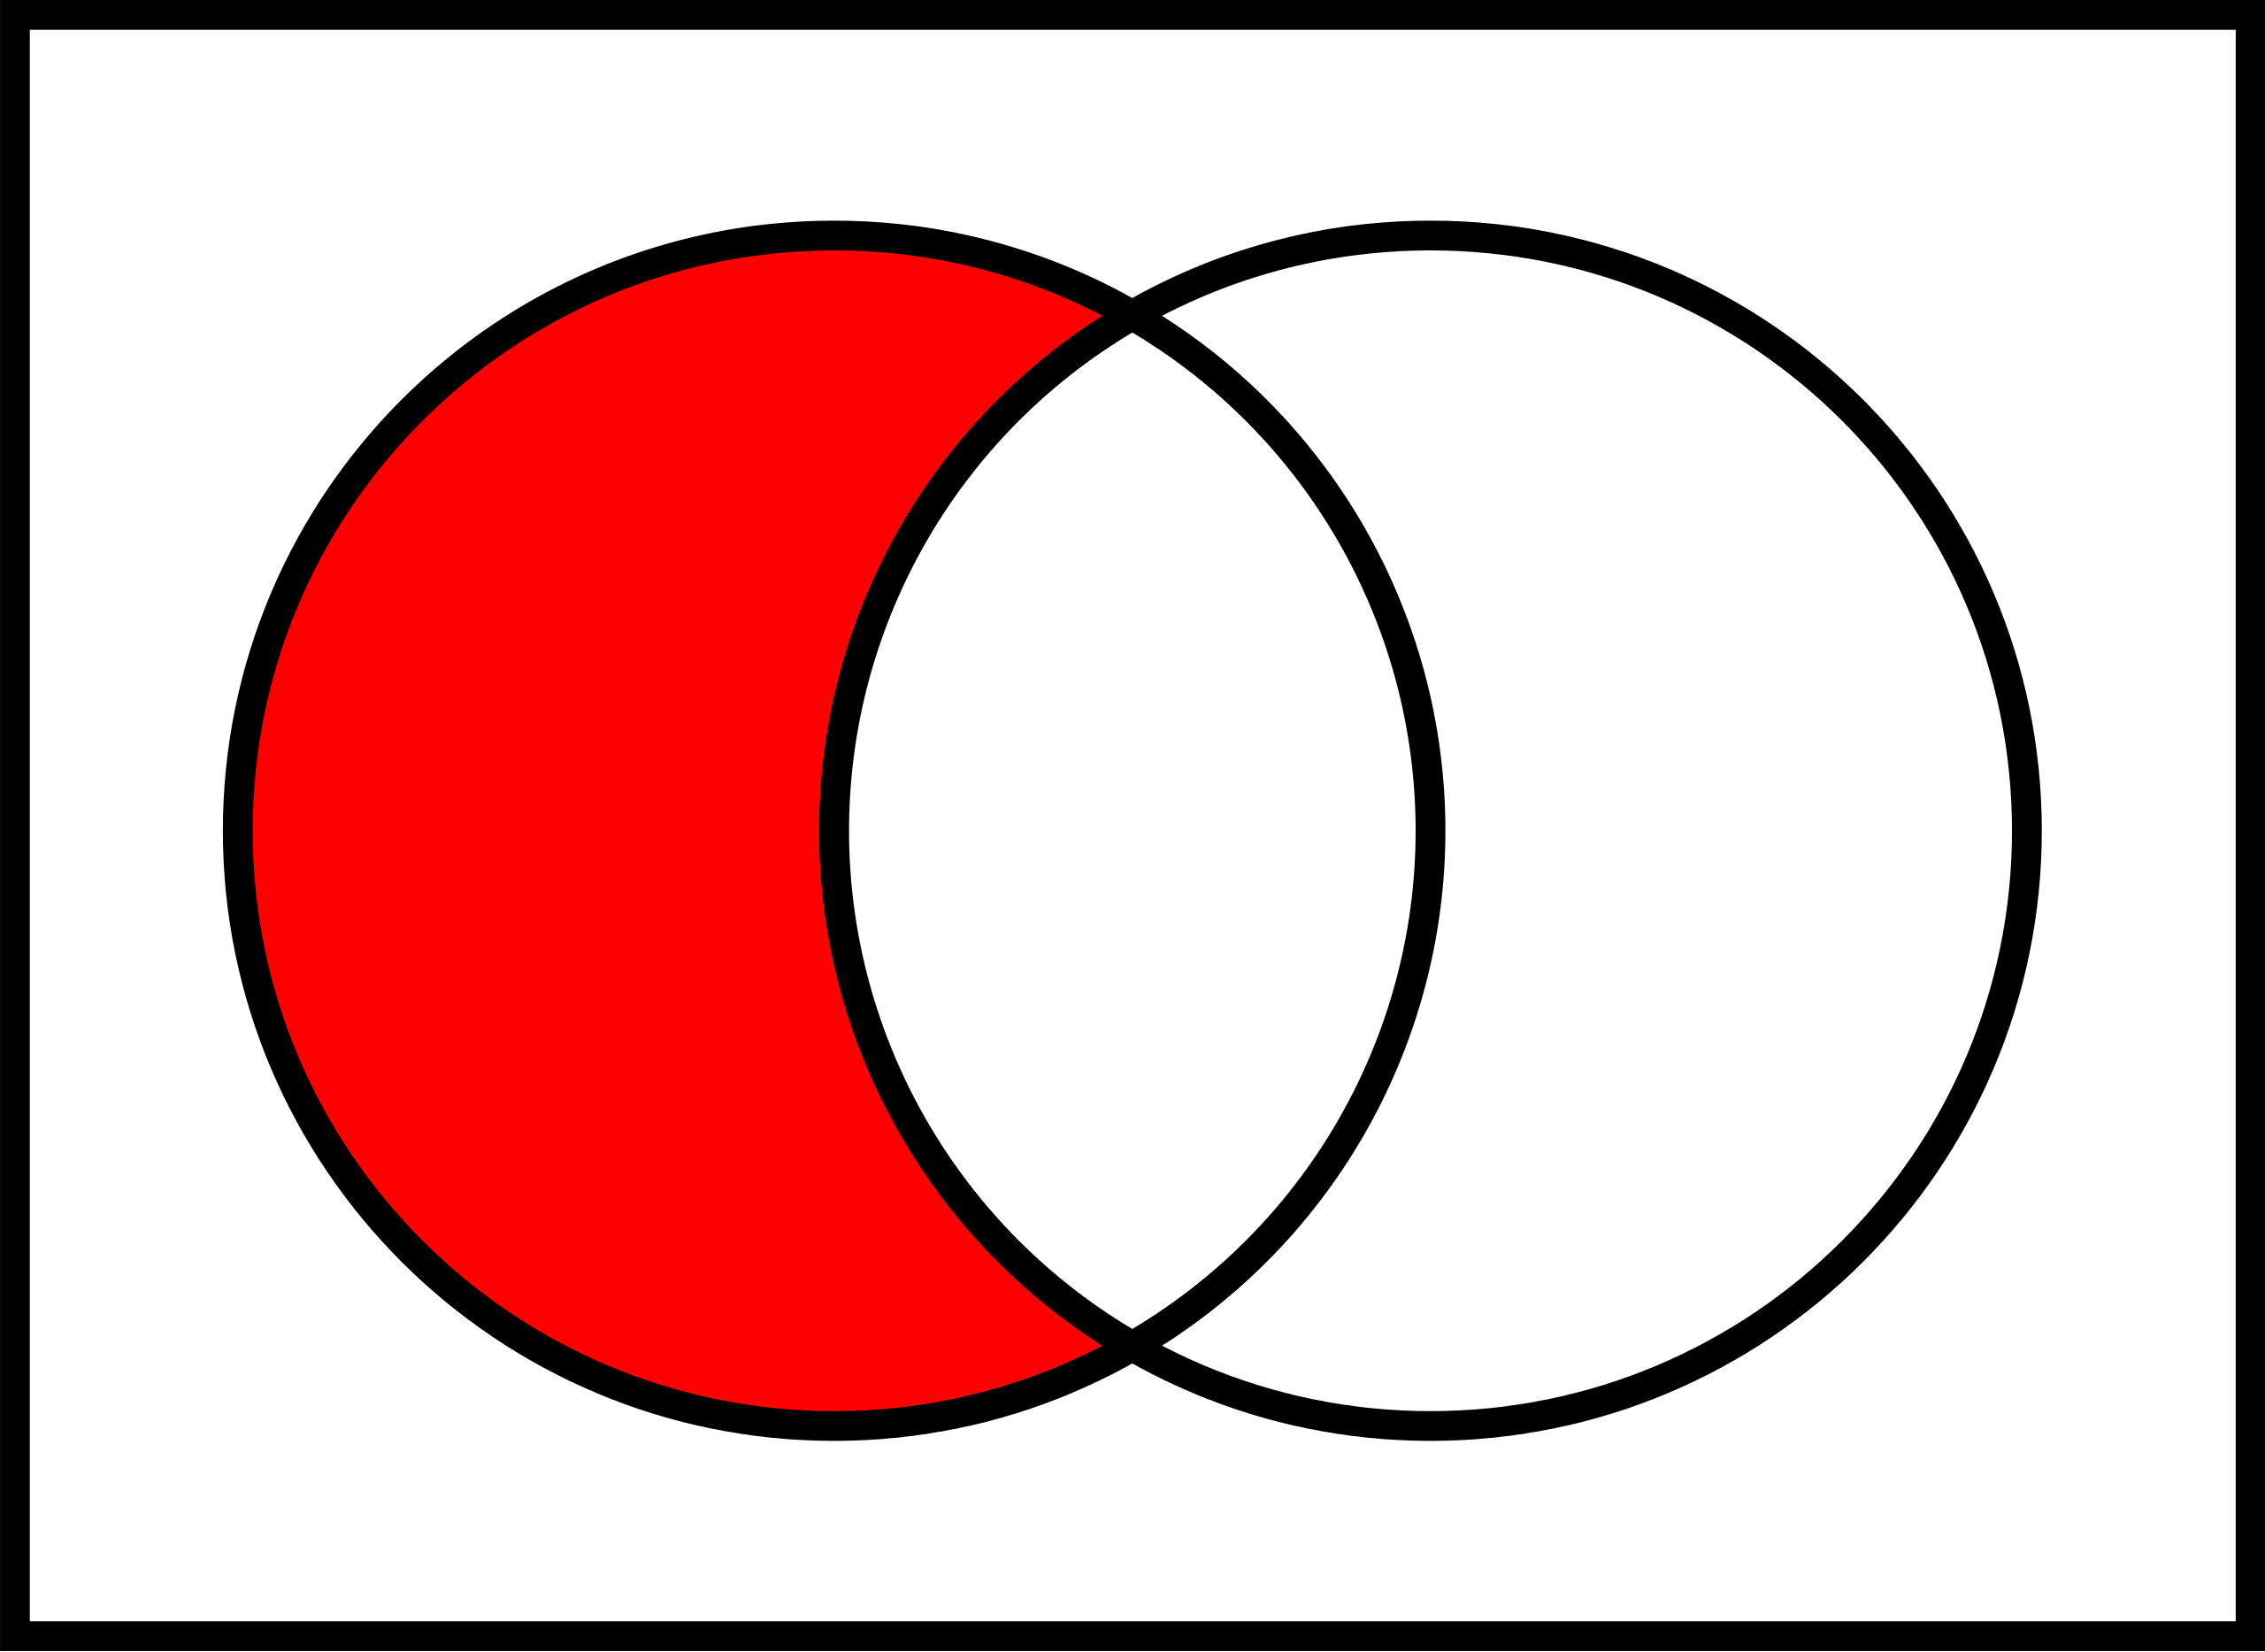
\includegraphics{./img/Venn0100.svg.png}

}

\caption{\(A \setminus B\)}

}

\end{minipage}%

\caption{\label{fig-sets}Typische Mengenoperationen}

\end{figure}

\hypertarget{disjunkte-ereignisse}{%
\subsubsection{Disjunkte Ereignisse}\label{disjunkte-ereignisse}}

(Engl. disjoint events)

\(A= \{1,2,3\}; B= \{4,5,6\}\)

\(A\) und \(B\) sind disjunkt: ihre Schnittmenge ist leer:
\(A \cap B = \emptyset\), s. Abbildung~\ref{fig-disjunkt}

\begin{figure}

{\centering 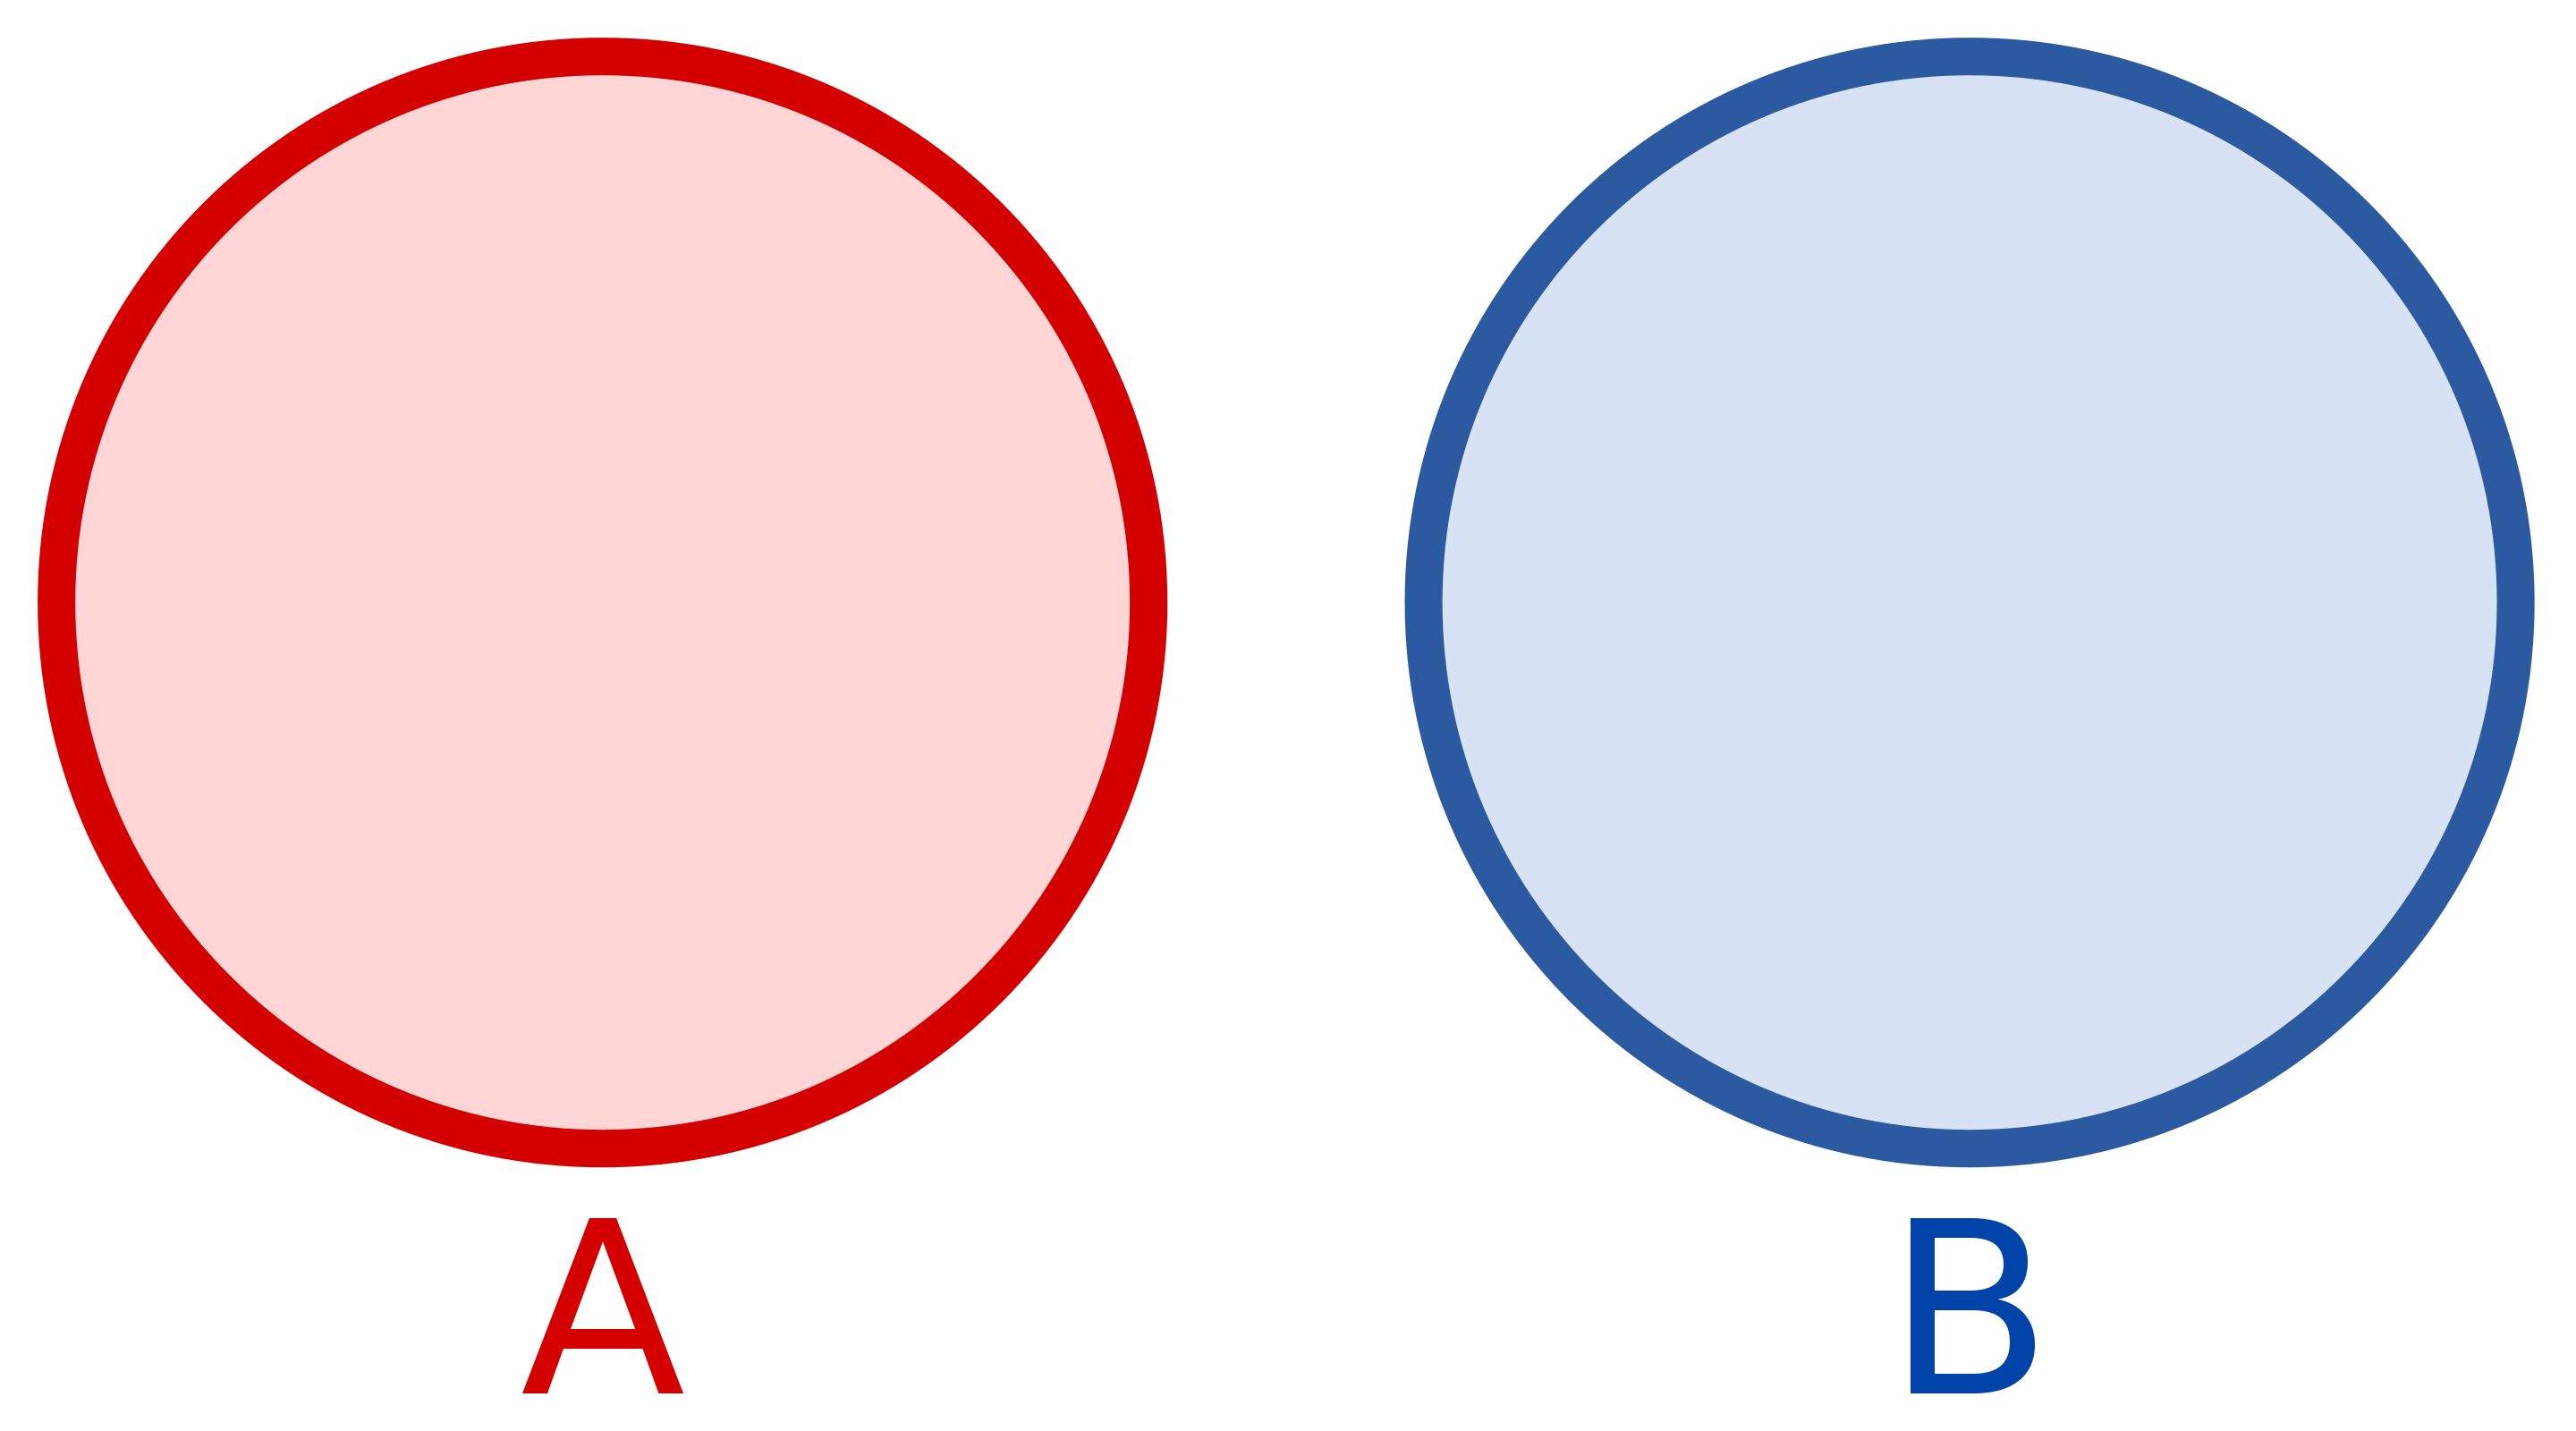
\includegraphics[width=0.25\textwidth,height=\textheight]{./img/2880px-Disjunkte_Mengen.svg.png}

}

\caption{\label{fig-disjunkt}Zwei disunkte Ereignisse, dargestellt noch
überlappungsfreie Kreise}

\end{figure}

\hypertarget{eselsbruxfccke-zur-vereinigungs--und-schnittmenge}{%
\subsubsection{Eselsbrücke zur Vereinigungs- und
Schnittmenge}\label{eselsbruxfccke-zur-vereinigungs--und-schnittmenge}}

Das Zeichen für eine Vereinigung zweier Mengen kann man leicht mit dem
Zeichen für einen Schnitt zweier Mengen leicht verwechseln; daher kommt
eine Eselbrücke gelesen, s. Abbildung~\ref{fig-esel}.

\begin{figure}

{\centering 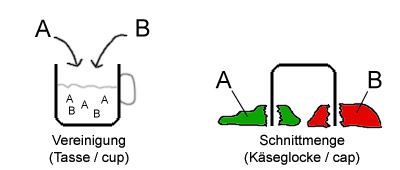
\includegraphics[width=0.55\textwidth,height=\textheight]{./img/ven_cup_cap.jpeg}

}

\caption{\label{fig-esel}Eselsbrücke für Vereinigungs- und Schnittmenge}

\end{figure}

\href{http://www.rither.de/a/mathematik/stochastik/mengentheorie-und-venn-diagramme/}{Quelle:
rither.de}

\hypertarget{animationen}{%
\subsubsection{Animationen}\label{animationen}}

\href{https://seeing-theory.brown.edu/compound-probability/index.html}{Animation
zu Mengenoperationen}

\href{https://www.geogebra.org/m/GEZV4xXc\#material/cmXR8fHN}{Animation
zur Vereinigung von Mengen}

\href{Geogebra,\%20J.\%20Merschhemke}{Quelle}

\hypertarget{additionssatz}{%
\subsection{Additionssatz}\label{additionssatz}}

Der Additionssatz wird verwendet, wenn wir an der Wahrscheinlichkeit
interessiert sind, dass \emph{mindestens eines der Ereignisse} eintritt.

\hypertarget{diskunkte-ereignisse}{%
\subsubsection{Diskunkte Ereignisse}\label{diskunkte-ereignisse}}

\(\Omega = {1,2,3,4,5,6}\)

\(\boxed{1\; 2\; 3\; 4\; 5\; 6}\)

Gesucht sei die Wahrscheinlichkeit des Ereignis \(A=\{1,2\}\).

\(\boxed{\boxed{1\; 2}\; \color{gray}{ 3\; 4\; 5\; 6}}\)

\(P(1 \cup 2) = \frac{1}{6} + \frac{1}{6} = \frac{2}{6}\)

\hypertarget{allgemein-disjunkt-oder-nicht-disjunkt}{%
\subsubsection{Allgemein (disjunkt oder nicht
disjunkt)}\label{allgemein-disjunkt-oder-nicht-disjunkt}}

Bei der Addition der Wahrscheinlichkeiten für \(A\) und \(B\) wird der
Schnitt \(A\cap B\) doppelt erfasst. Er muss daher noch abgezogen werden
(vgl. Abbildung~\ref{fig-sets2}):

\[P(A \cup B) = P(A) + P(B) - P(A\cap B)\]

\begin{figure}

\begin{minipage}[t]{0.50\linewidth}

{\centering 

\raisebox{-\height}{

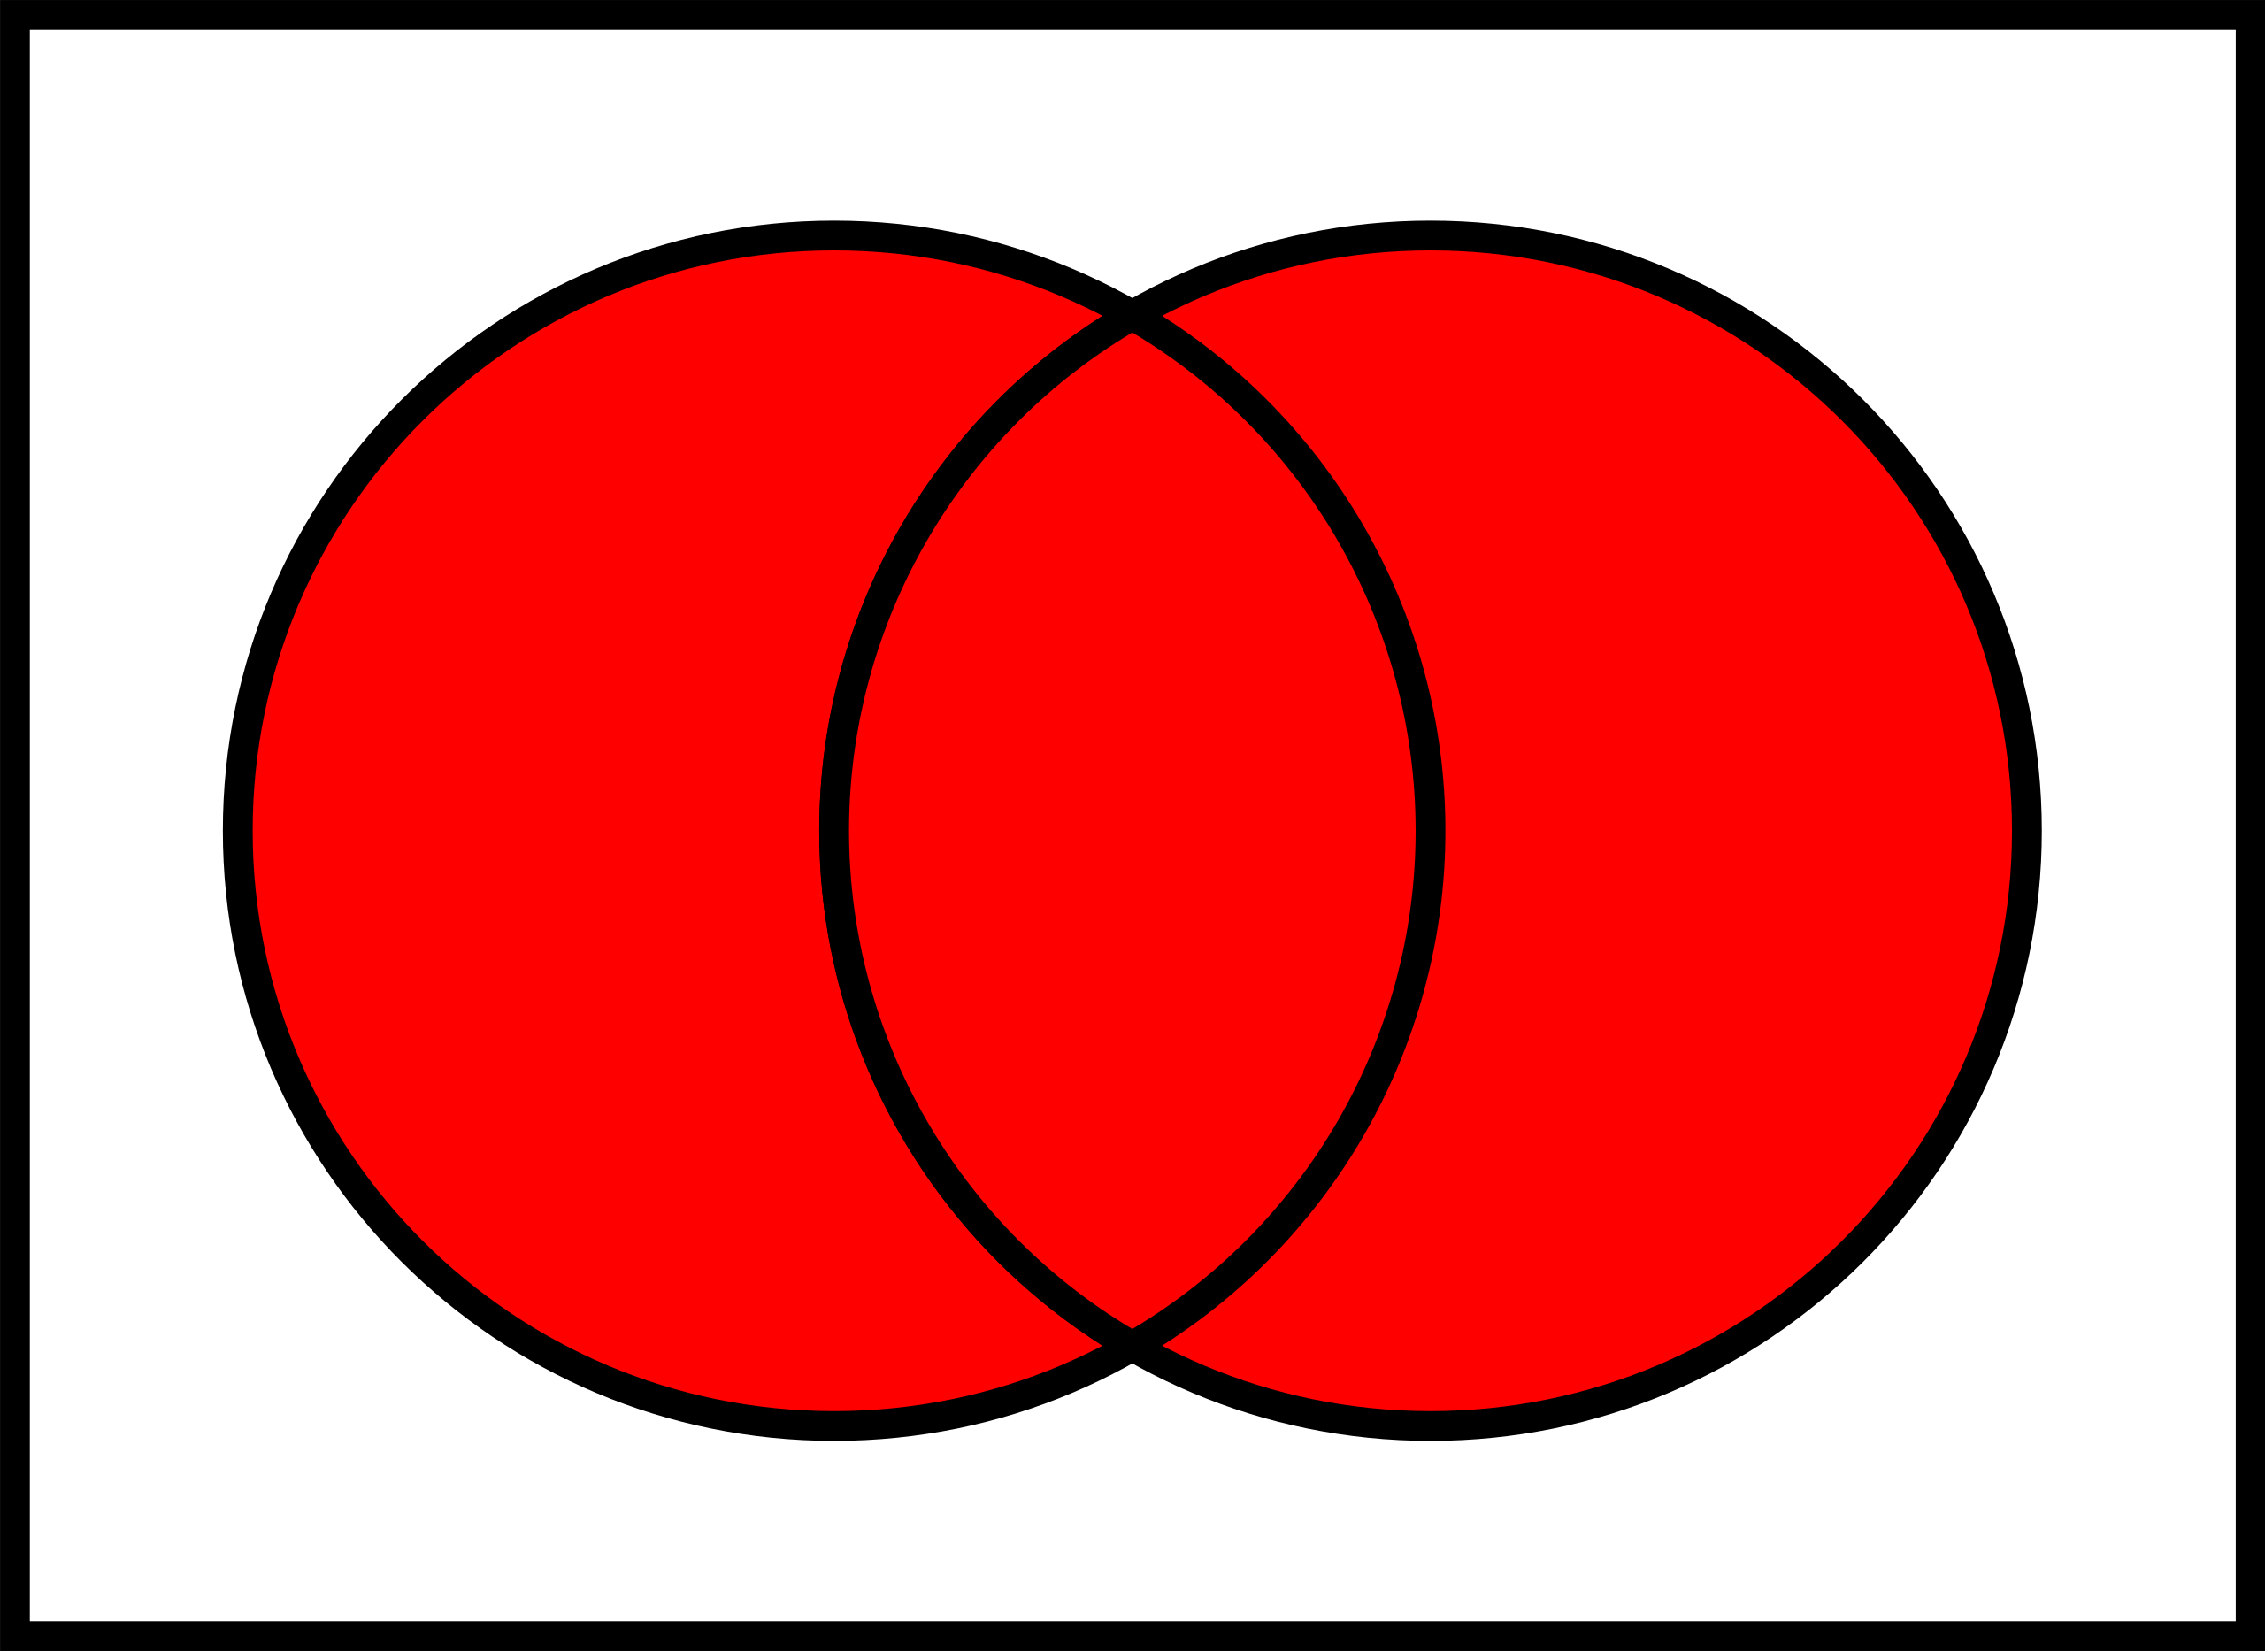
\includegraphics{./img/Venn0111.svg.png}

}

\caption{\(A \cup B\)}

}

\end{minipage}%
%
\begin{minipage}[t]{0.50\linewidth}

{\centering 

\raisebox{-\height}{

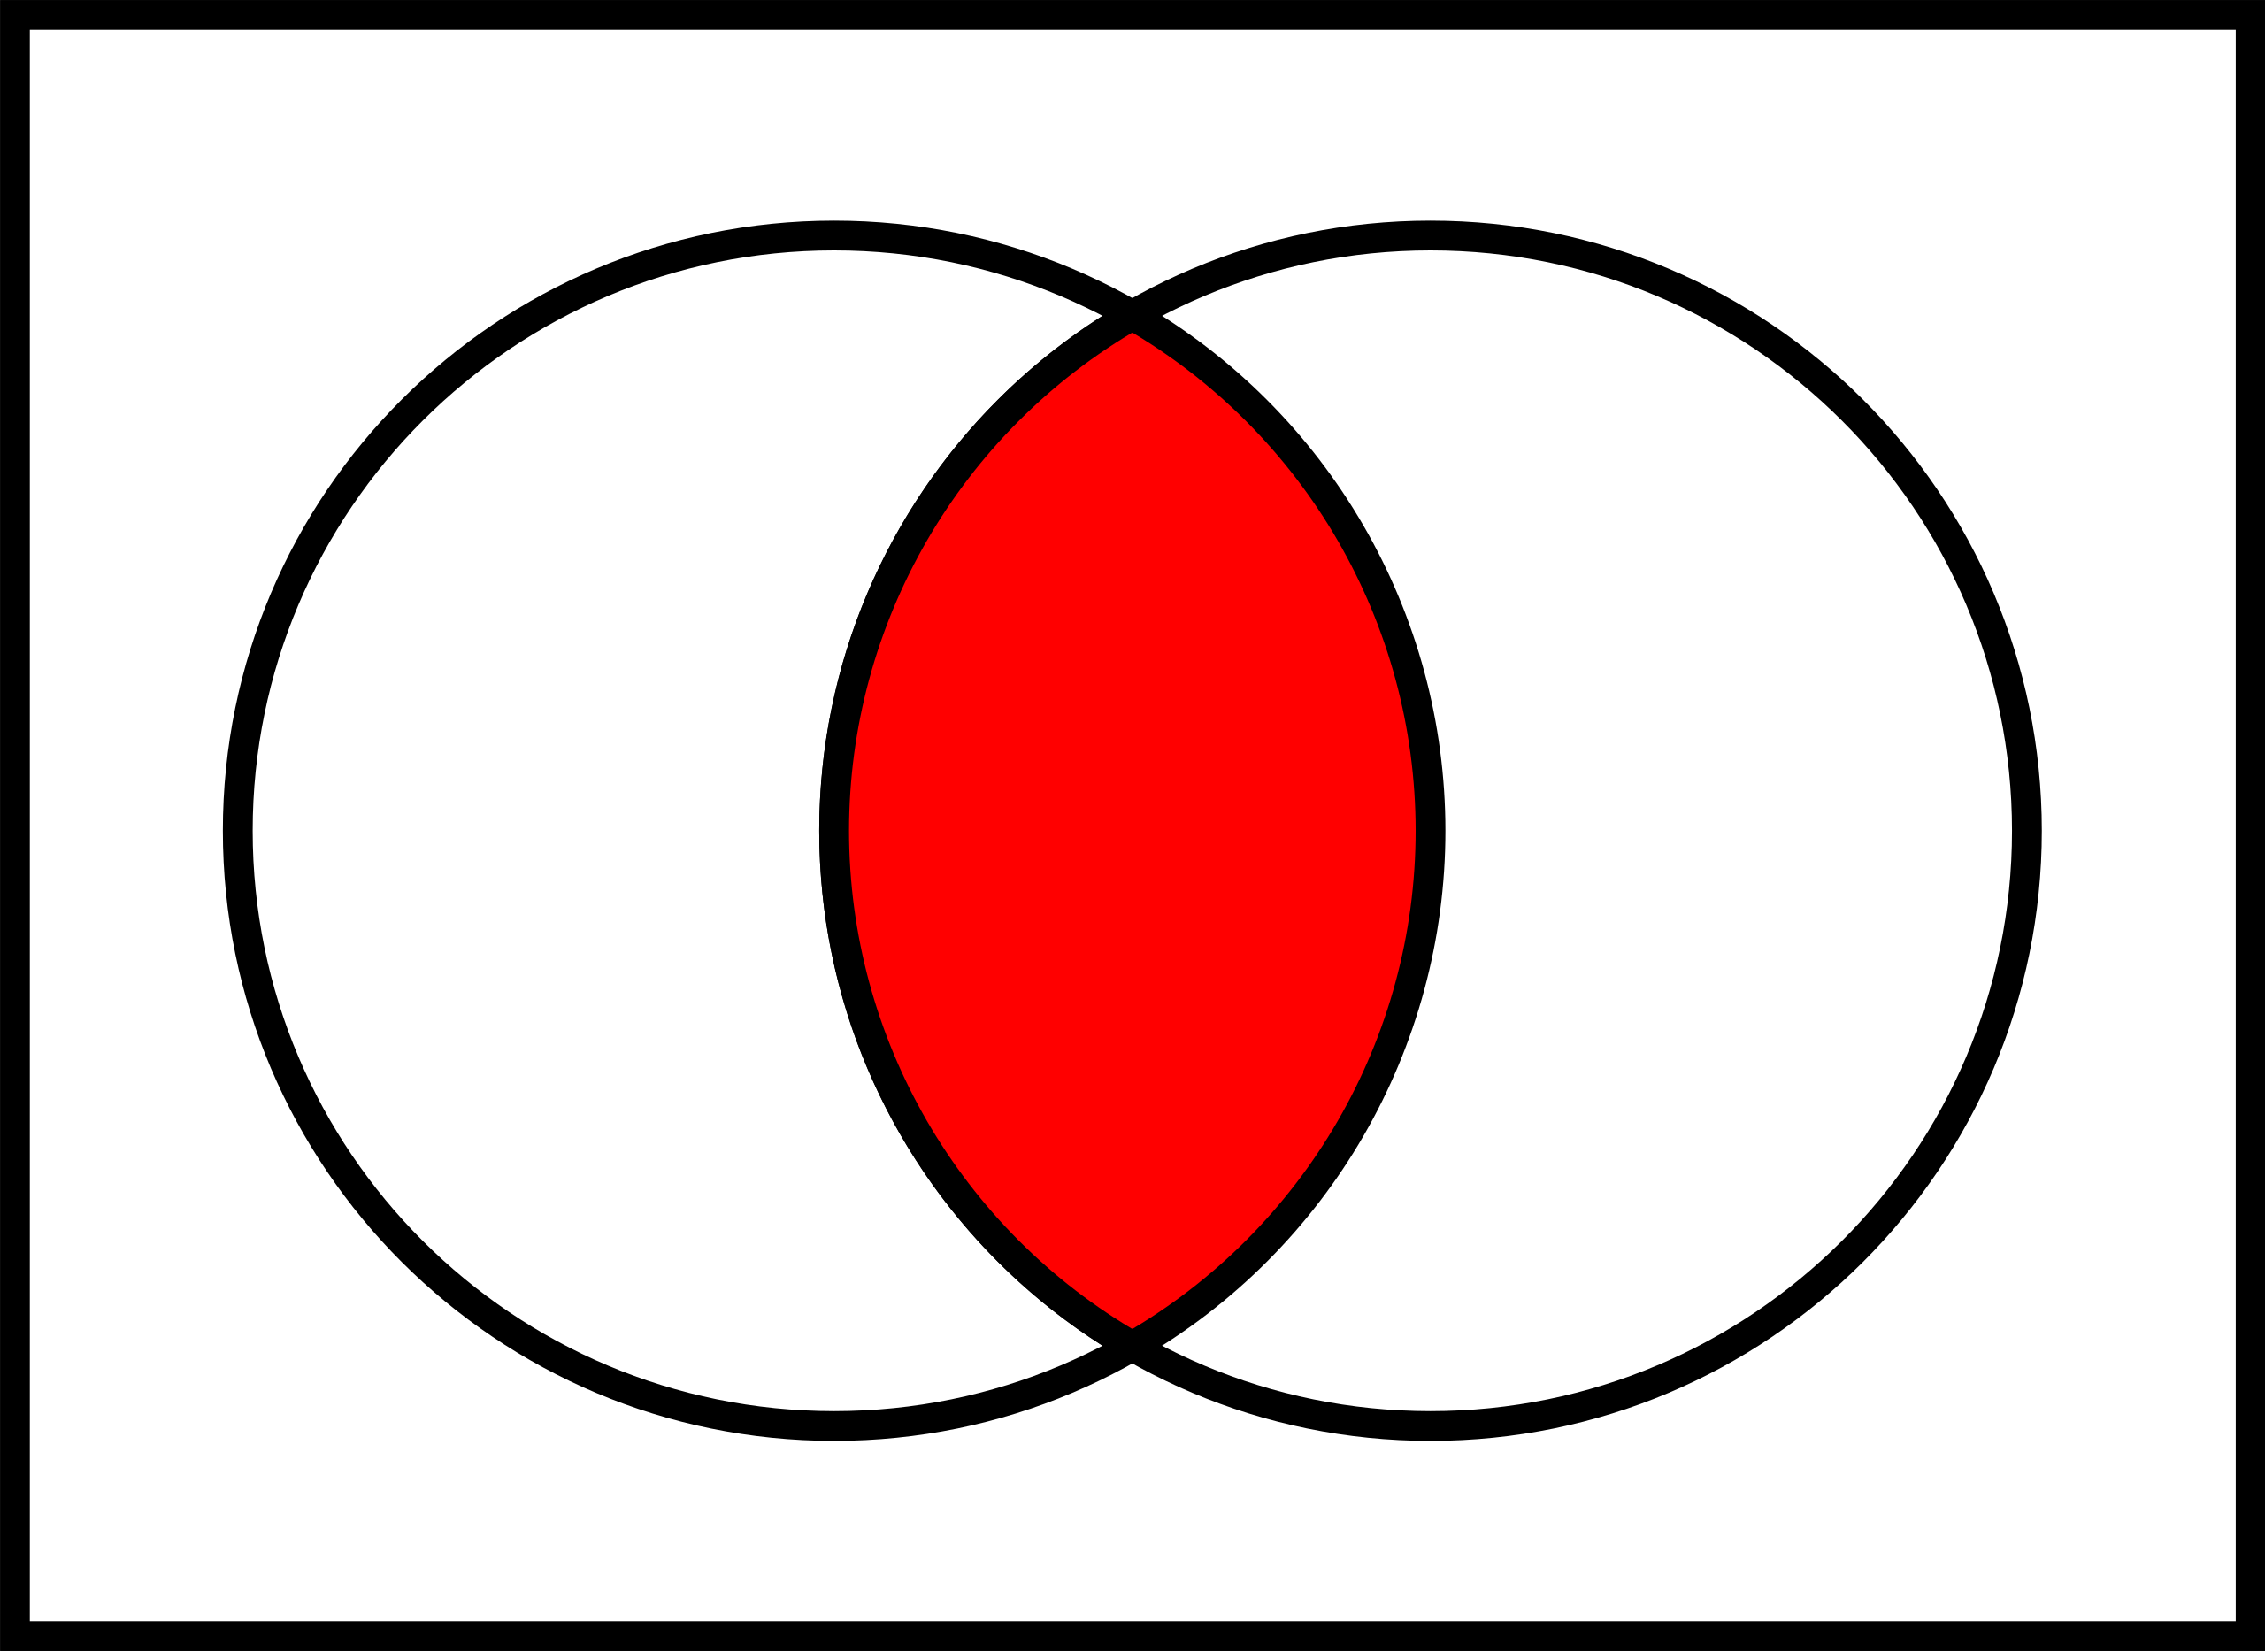
\includegraphics{./img/Venn0001.svg.png}

}

\caption{\(A \cap B\)}

}

\end{minipage}%

\caption{\label{fig-sets2}Die Schnittmenge muss beim Vereinigen
abgezogen werden, damit sie nicht doppelt gezählt wird.}

\end{figure}

\hypertarget{bedingte-wahrscheinlichkeit}{%
\subsection{Bedingte
Wahrscheinlichkeit}\label{bedingte-wahrscheinlichkeit}}

\hypertarget{animation}{%
\subsubsection{Animation}\label{animation}}

Schauen Sie sich mal diese
\href{https://setosa.io/conditional/}{Wahnsinnsanimation von Victor
Powell an}. Hammer!

\hypertarget{schema}{%
\subsubsection{Schema}\label{schema}}

Abb. Abbildung~\ref{fig-schema-p} illustriert gemeinsame
Wahrscheinlichkeit, \$P(A \cap B) und bedingte Wahrscheinlichkeit,
\(P(A|B)\).

\begin{figure}

{\centering 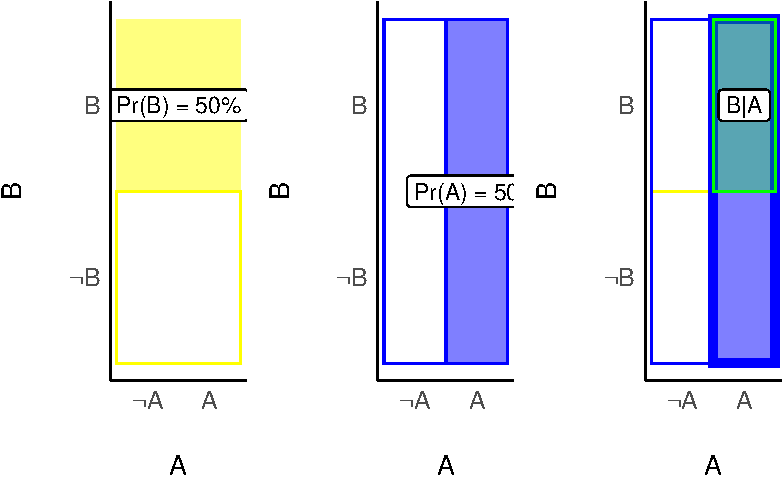
\includegraphics{./Wskt_files/figure-pdf/fig-schema-p-1.pdf}

}

\caption{\label{fig-schema-p}Illustration von gemeinsamer und bedingter
Wahrscheinlichkeit}

\end{figure}

Bedingte Wahrscheinlichkeit ist vergleichbar zu Filtern einer Tabelle:

\begin{Shaded}
\begin{Highlighting}[]
\NormalTok{d }\OtherTok{\textless{}{-}} 
\NormalTok{  tibble}\SpecialCharTok{::}\FunctionTok{tribble}\NormalTok{(}
      \SpecialCharTok{\textasciitilde{}}\NormalTok{id, }\SpecialCharTok{\textasciitilde{}}\NormalTok{A, }\SpecialCharTok{\textasciitilde{}}\NormalTok{B,}
      \StringTok{"1"}\NormalTok{, 0L, 0L,}
      \StringTok{"2"}\NormalTok{, 0L, 1L,}
      \StringTok{"3"}\NormalTok{, 1L, 0L,}
      \StringTok{"4"}\NormalTok{, 1L, 1L,}
  \StringTok{"SUMME"}\NormalTok{, 2L, 2L}
\NormalTok{  )}
\end{Highlighting}
\end{Shaded}

Es ergeben sich folgende Wahrscheinlichkeiten:

\(P(A) = 2/4\)

\(P(B) = 2/4\)

\(P(A \cap B) = 1/4\)

\(P(A|B) = 1/2\)

\hypertarget{un-abhuxe4ngigkeit}{%
\subsection{(Un-)Abhängigkeit}\label{un-abhuxe4ngigkeit}}

Stochastische Unabhängigkeit ist ein Spezialfall von Abhängigkeit: Es
gibt sehr viele Ausprägungen für Abhängigkeit, aber nur eine für
Unabhängigkeit. Können wir Unabhängigkeit nachweisen, haben wir also
eine starke Aussage getätigt.

\emph{Abhängig}, s. Abbildung~\ref{fig-abh}, links: Überleben auf der
Titanic ist offenbar \emph{abhängig} von der Passagierklasse. Auf der
anderen Seite: Das Ereignis \emph{Überleben} auf der Titanic ist
\emph{un}abhängig vom Ereignis \emph{Alter ist eine Primzahl}, s.
Abbildung~\ref{fig-abh}, rechts.

\begin{figure}

{\centering 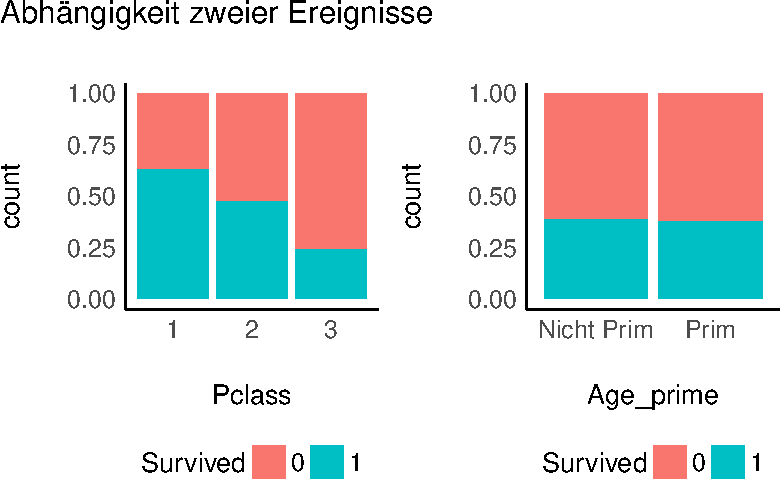
\includegraphics[width=1\textwidth,height=\textheight]{./Wskt_files/figure-pdf/fig-abh-1.pdf}

}

\caption{\label{fig-abh}Abhängigkeit und Unabhängigkeit zweier
Ereignisse}

\end{figure}

Zur Ab- bzw. Un-Abhängigkeit zweier Variablen, an Beispielen
illustriert.

\leavevmode\vadjust pre{\hypertarget{exm-covid}{}}%
\begin{example}[Zusammenhang von Covidsterblichkeit und
Impfquote]\label{exm-covid}

Sind die Ereignisse \emph{Tod durch Covid} bzw. \emph{Impfquote} (\(A\))
und \emph{Land}\footnote{hier mit den zwei Ausprägungen \emph{DEU} und
  \emph{USA}} (\(B\)) voneinander abhängig (Abb.
Abbildung~\ref{fig-covid1})?

\begin{figure}

{\centering 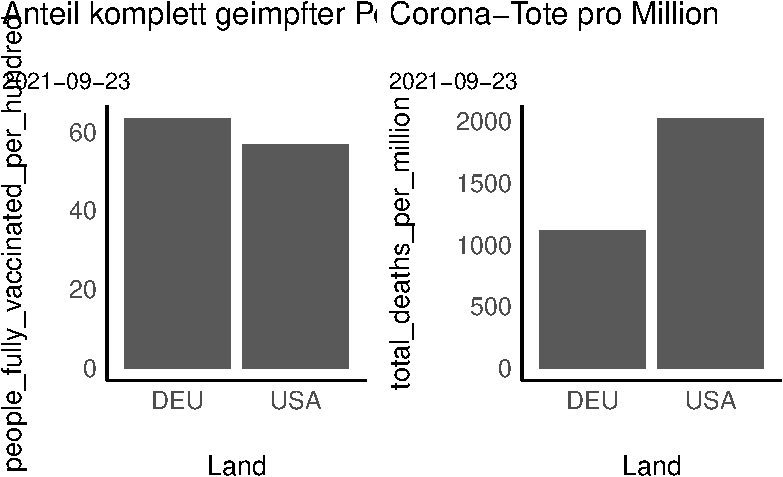
\includegraphics{./Wskt_files/figure-pdf/fig-covid1-1.pdf}

}

\caption{\label{fig-covid1}Impfquote und Sterblichkeit sind voneinander
abhängig (bezogen auf Covid, auf Basis vorliegender Daten)}

\end{figure}

Ja, da in beiden Diagrammen gilt: \(P(A|B) \ne Pr(A) \ne Pr(A|\neg B)\).

Daten von \href{https://ourworldindata.org/covid-deaths}{Our World in
Data}.

\end{example}

\hypertarget{multiplikationssatz}{%
\subsection{Multiplikationssatz}\label{multiplikationssatz}}

Der Multiplikationssatz wird verwendet, wenn wir an der
Wahrscheinlichkeit interessiert sind, dass \emph{alle Ereignisse}
eintreten.

\hypertarget{unabhuxe4ngige-ereignisse}{%
\subsubsection{Unabhängige Ereignisse}\label{unabhuxe4ngige-ereignisse}}

Wir werfen eine faire Münze \emph{zwei} Mal (Abb.
Abbildung~\ref{fig-2muenzen}).

\begin{figure}

{\centering 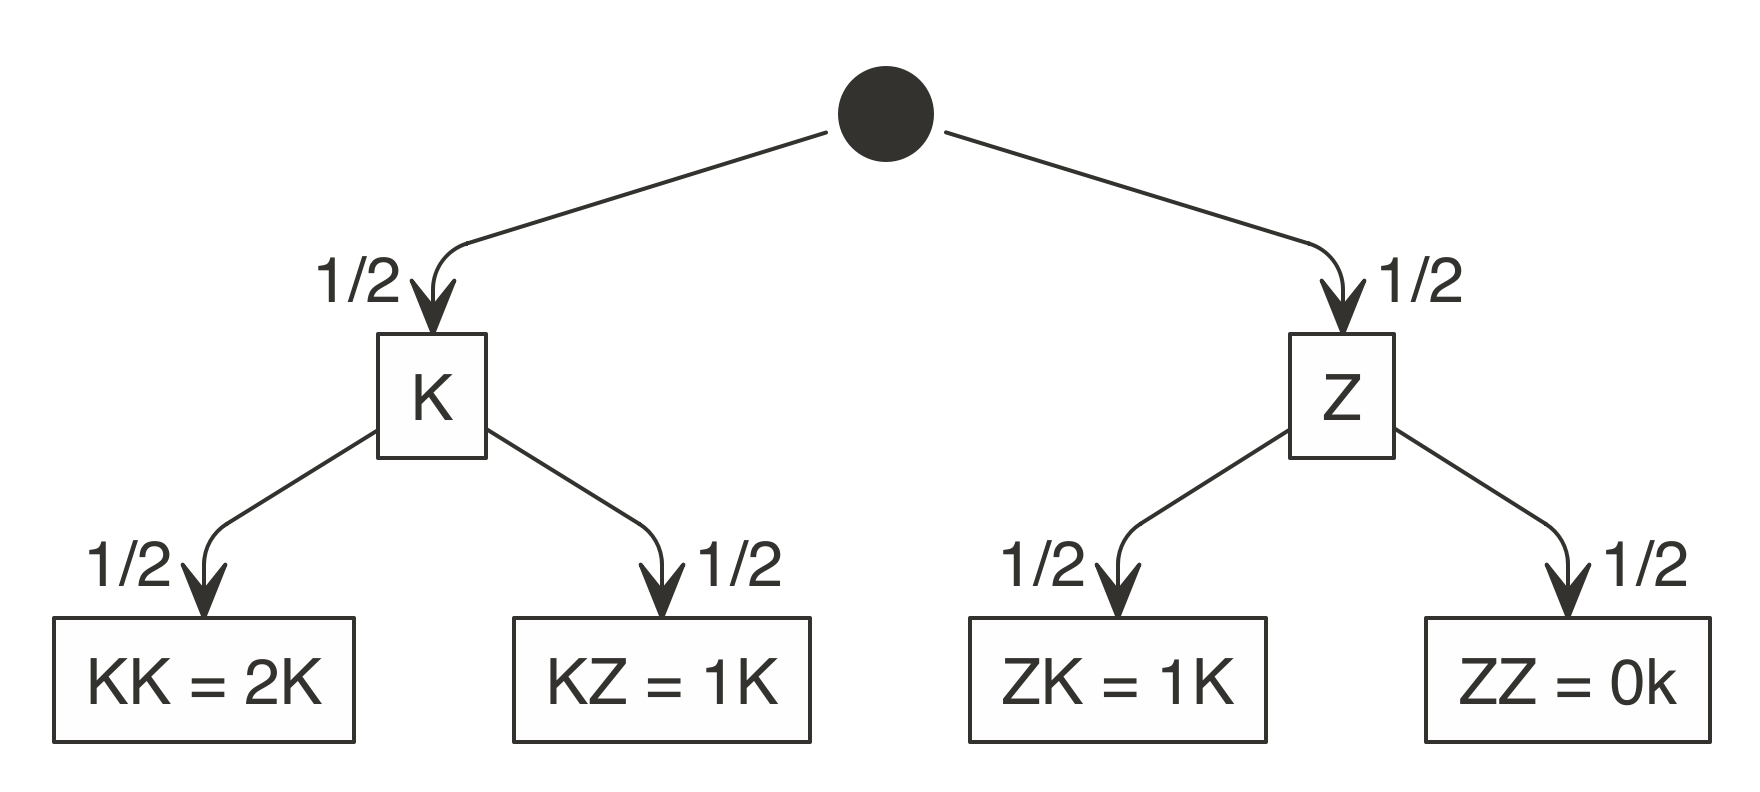
\includegraphics{./img/muenz1.png}

}

\caption{\label{fig-2muenzen}Wir werfen 2 faire Münzen}

\end{figure}

Abb. Abbildung~\ref{fig-2muenzen} zeigt ein \emph{Baumdiagramm}. Jeder
\emph{Kasten} (Knoten) zeigt ein \emph{Ergebnis.} Die Pfeile (Kanten)
symbolisieren die Abfolge des Experiments: Vom ``Start'' (schwarzer
Kreis) führen zwei mögliche Ergebniss ab, jeweils mit Wahrscheinlichkeit
1/2. Die untersten Knoten nennt man auch \emph{Blätter} (Endknoten), sie
zeigen das Endresultat des (in diesem Fall) zweifachen Münzwurfs. Der
Weg vom Start zu einem bestimmten Blatt nennt man \emph{Pfad}. Die
Anzahl der Pfade entspricht der Anzahl der Blätter. In diesen Diagramm
gibt es vier Pfade (und Blätter).

\begin{longtable}[]{@{}ll@{}}
\toprule()
Ereignis & Pr \\
\midrule()
\endhead
0K & 1/2 * 1/2 = 1/4 \\
1K & 1/4 + 1/4 = 1/2 \\
2K & 1/2 * 1/2 = 1/4 \\
\bottomrule()
\end{longtable}

Wir werfen eine faire Münze \emph{drei} Mal (Abb.
Abbildung~\ref{fig-3muenzen})

\begin{figure}

{\centering 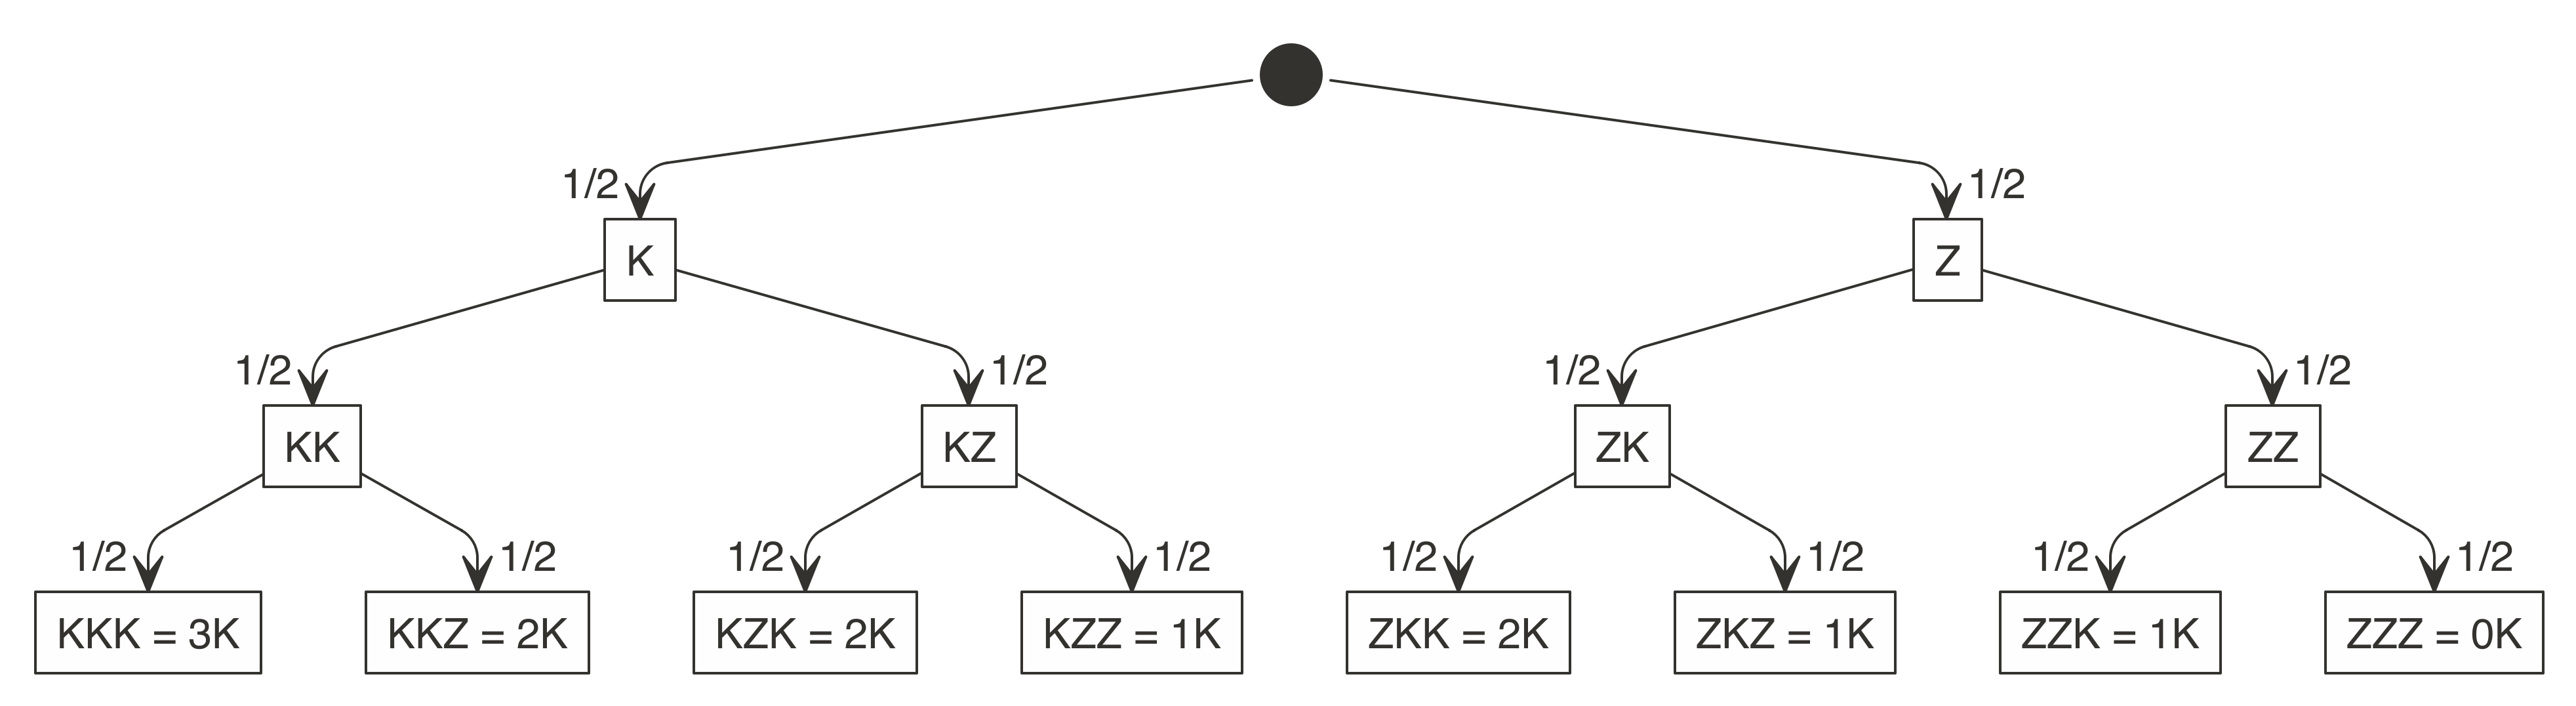
\includegraphics{./img/muenz2.png}

}

\caption{\label{fig-3muenzen}Wir werfen drei faire Münzen}

\end{figure}

\begin{longtable}[]{@{}ll@{}}
\toprule()
Ereignis & Pr \\
\midrule()
\endhead
0K & 1/2 * 1/2 * 1/2 = 1/8 \\
1K & 1/8 + 1/8 + 1/8 = 3/8 \\
2K & 3 * 1/8 = 3/8 \\
3K & 1/2 * 1/2 * 1/2 = 1/8 \\
\bottomrule()
\end{longtable}

\(Pr(AB) = Pr(A) \cdot Pr(B) = 50\% \cdot 50\% = 25\%\)

\begin{figure}

{\centering 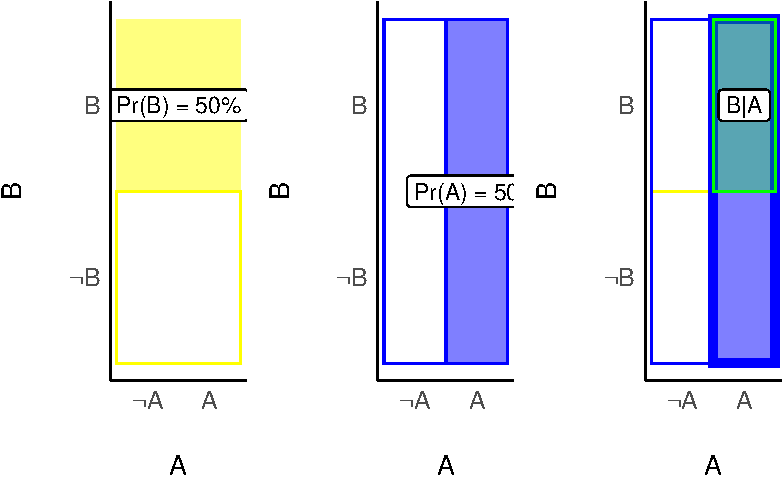
\includegraphics{./Wskt_files/figure-pdf/fig-unabh-e-1.pdf}

}

\caption{\label{fig-unabh-e}Unabhängige Ereignisse visualisiert}

\end{figure}

Abb. Abbildung~\ref{fig-unabh-e} zeigt, dass gilt:
\(P(A\cap B) = P(A) \cdot P(B) = P(B) \cdot P(A)\).

\hypertarget{kalt-und-regen}{%
\subsubsection{Kalt und Regen}\label{kalt-und-regen}}

Von McElreath (2020) stammt diese Verdeutlichung der gmeinsamen
Wahrscheinlichkeit:

Was ist die Wahrscheinlichkeit für \emph{kalt ❄ und Regen ⛈️}?

Die Wahrscheinlichkeit für kalt und Regen ist die Wahrscheinlichkeit von
\emph{Regen} ⛈, wenn's \emph{kalt} ❄ ist mal die Wahrscheinlichkeit von
\emph{Kälte} ❄.

Ebenfalls gilt:

Die Wahrscheinlichkeit für kalt und Regen ist die Wahrscheinlichkeit von
\emph{Kälte} ❄, wenn's \emph{regnet} ⛈️ mal die Wahrscheinlichkeit von
\emph{Regen} ⛈️.

Das Gesagte als Emoji-Gleichung:

\(P(❄️ und ⛈️) = P(⛈️ |❄️ ) \cdot P(❄️) = P(❄️ |⛈️ ) \cdot P(⛈️) = P(⛈️ und ❄️)\)

Allgemein:

\(P(A\cap B) = P(A) \cdot P(B|A) = P(B) \cdot P(A|B)\)

Man kann also die ``Gleichung drehen''.

\hypertarget{abhuxe4ngige-ereignisse}{%
\subsubsection{Abhängige Ereignisse}\label{abhuxe4ngige-ereignisse}}

Ein Baumdiagramm bietet sich zur Visualisierung abhängiger Ereignisse
an, s. Abb. Abbildung~\ref{fig-baum-abh}. Für unabhängige Ereignisse
übrigens auch.

In einer Urne befinden sich fünf Kugeln, von denen vier rot sind und
eine blau ist.

wie groß ist die Wahrscheinlichkeit, dass bei zwei Ziehungen ohne
Zurücklegen (\emph{ZOZ}) \emph{zwei rote Kugeln} gezogen werden (Bourier
2018), S. 47.

Hier ist unsere Urne:

\[\boxed{\color{red}{R, R, R, R}, \color{blue}B}\]

Und jetzt ziehen wir. Hier ist das Baumdiagramm, s. Abb.
Abbildung~\ref{fig-baum-abh}.

\begin{figure}

{\centering 

\begin{figure}[H]

{\centering 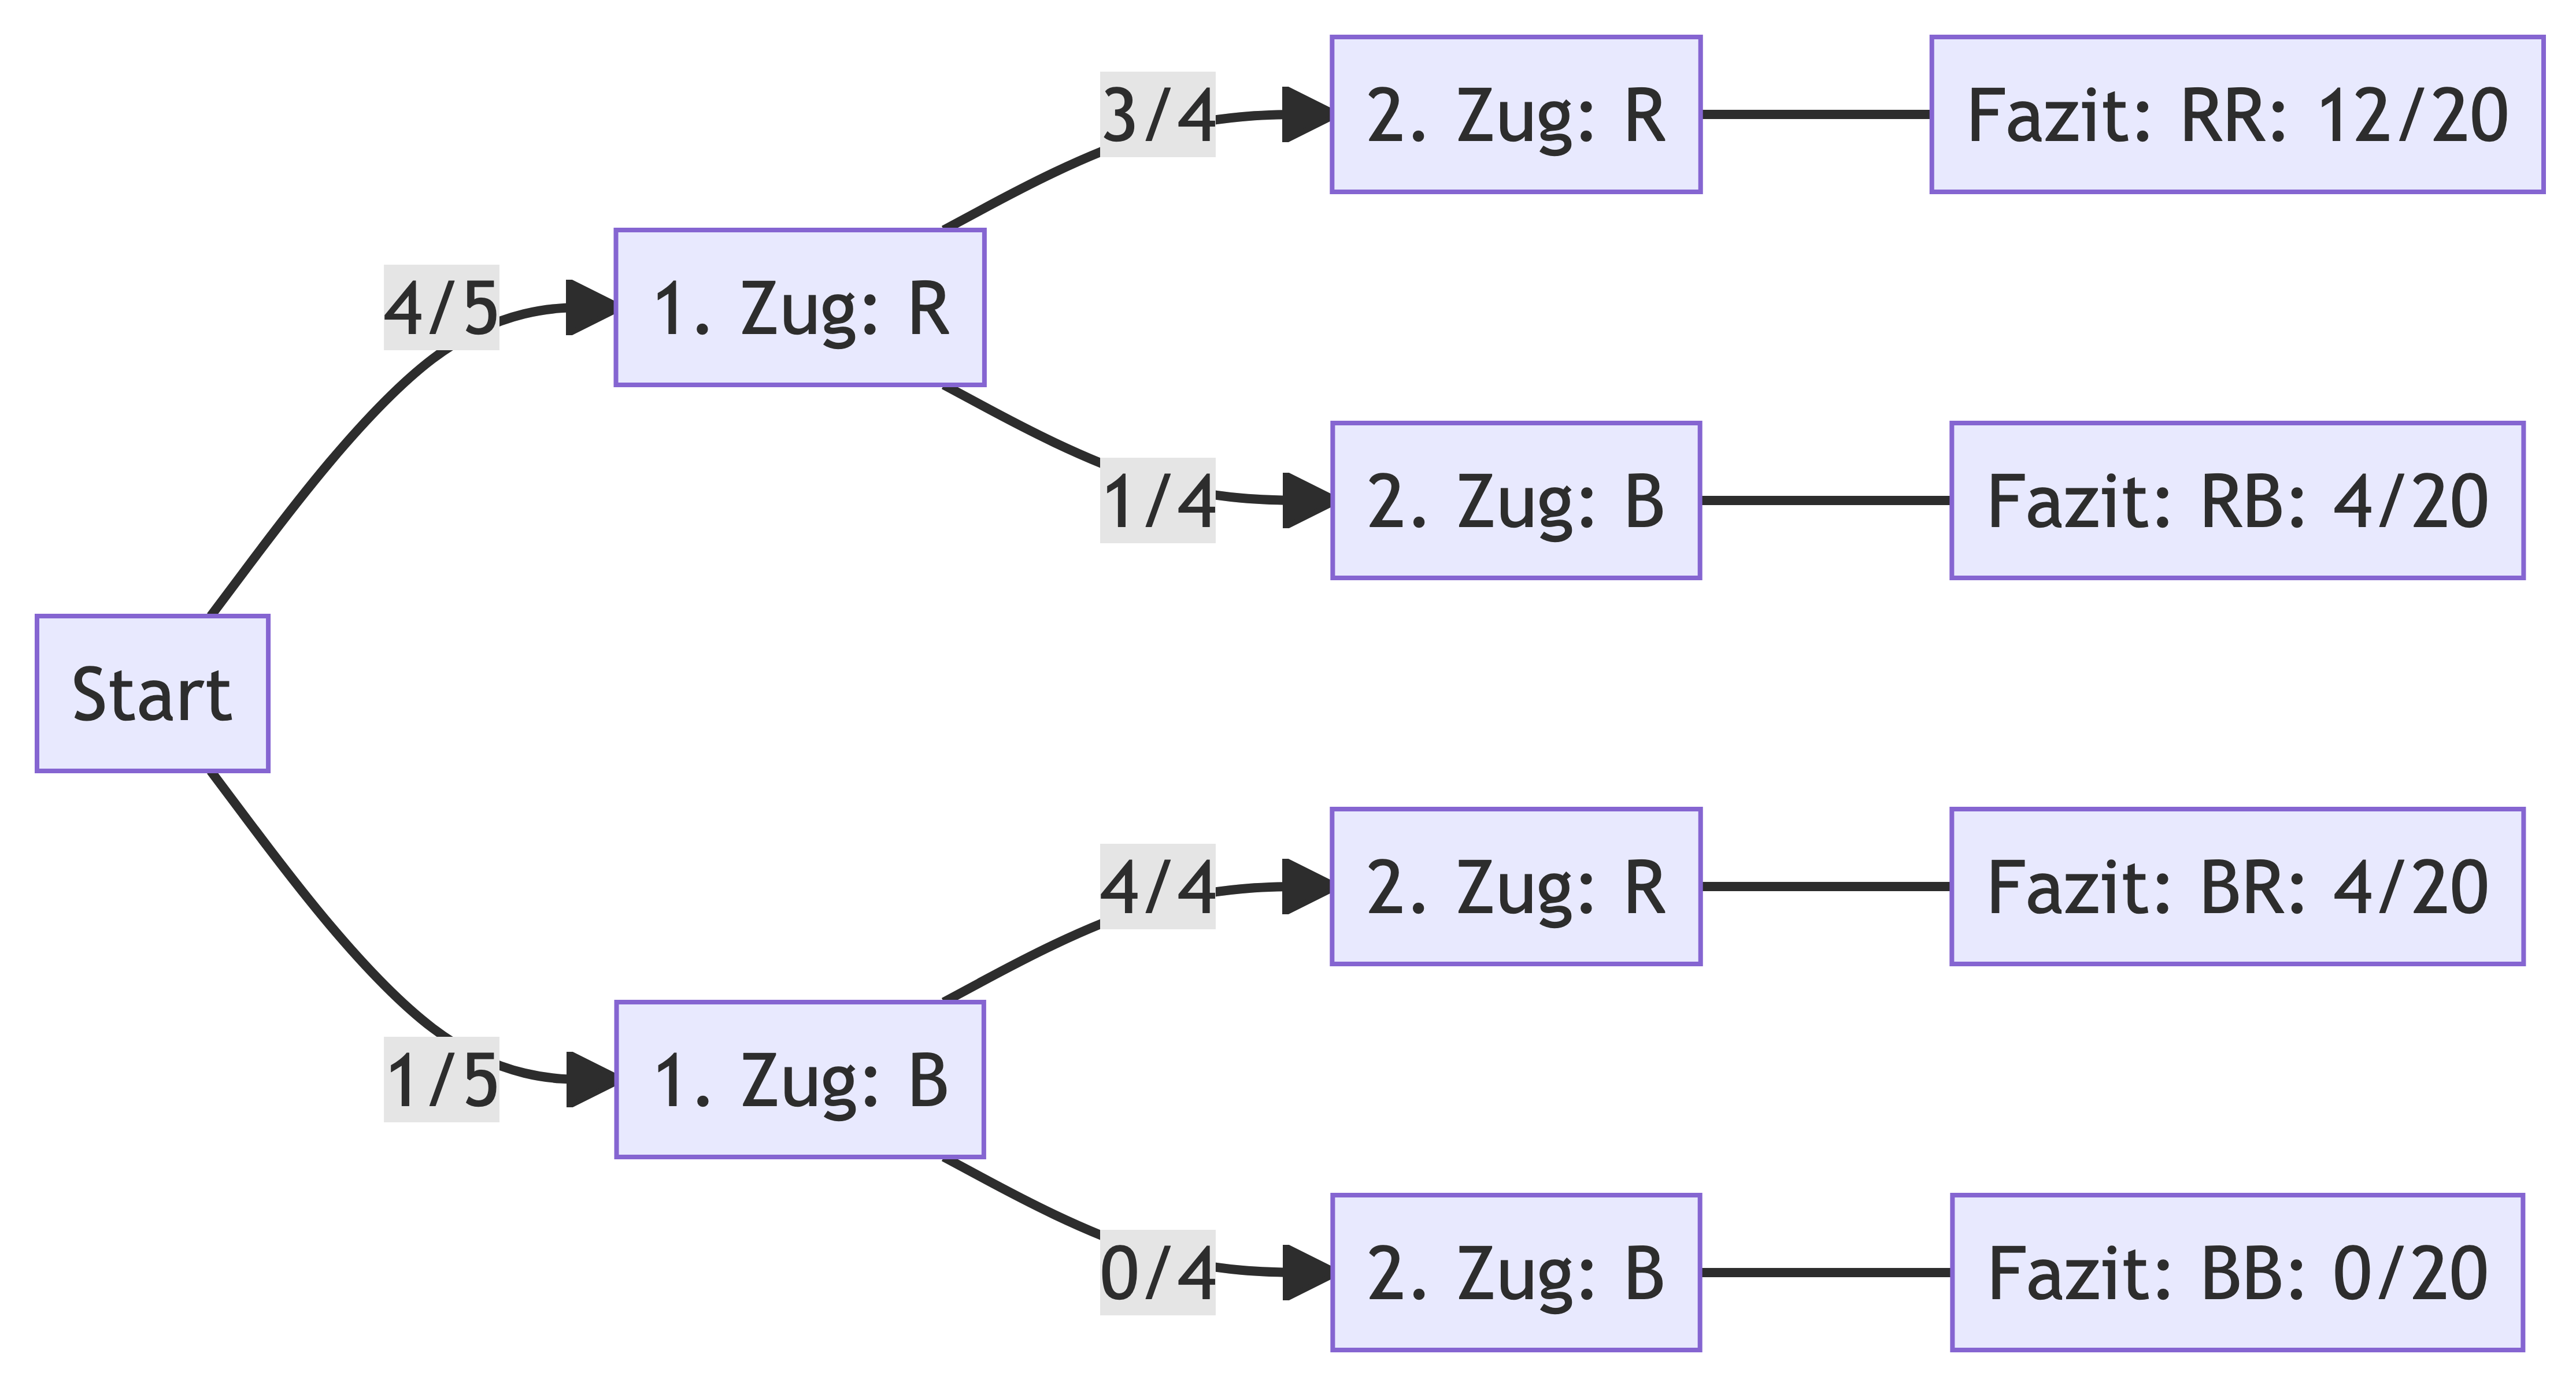
\includegraphics[width=5.81in,height=3.13in]{./Wskt_files/figure-latex/mermaid-figure-1.png}

}

\end{figure}

}

\caption{\label{fig-baum-abh}Baumdiagramm für ein ein zweistufiges
Zufallsereignis, wobei der 2. Zug (Stufe) abhängig ist vom 1. Zug.}

\end{figure}

Es gilt also: \(P(A\cap B) = P(A) \cdot P(B|A)\).

\hypertarget{totale-wahrscheinlichkeit}{%
\subsection{Totale Wahrscheinlichkeit}\label{totale-wahrscheinlichkeit}}

Abbildung~\ref{fig-tot-wskt} zeigt das Baumdiagramm für die Aufgabe
Bourier (2018), S. 56.

\begin{figure}

{\centering 

\begin{figure}[H]

{\centering 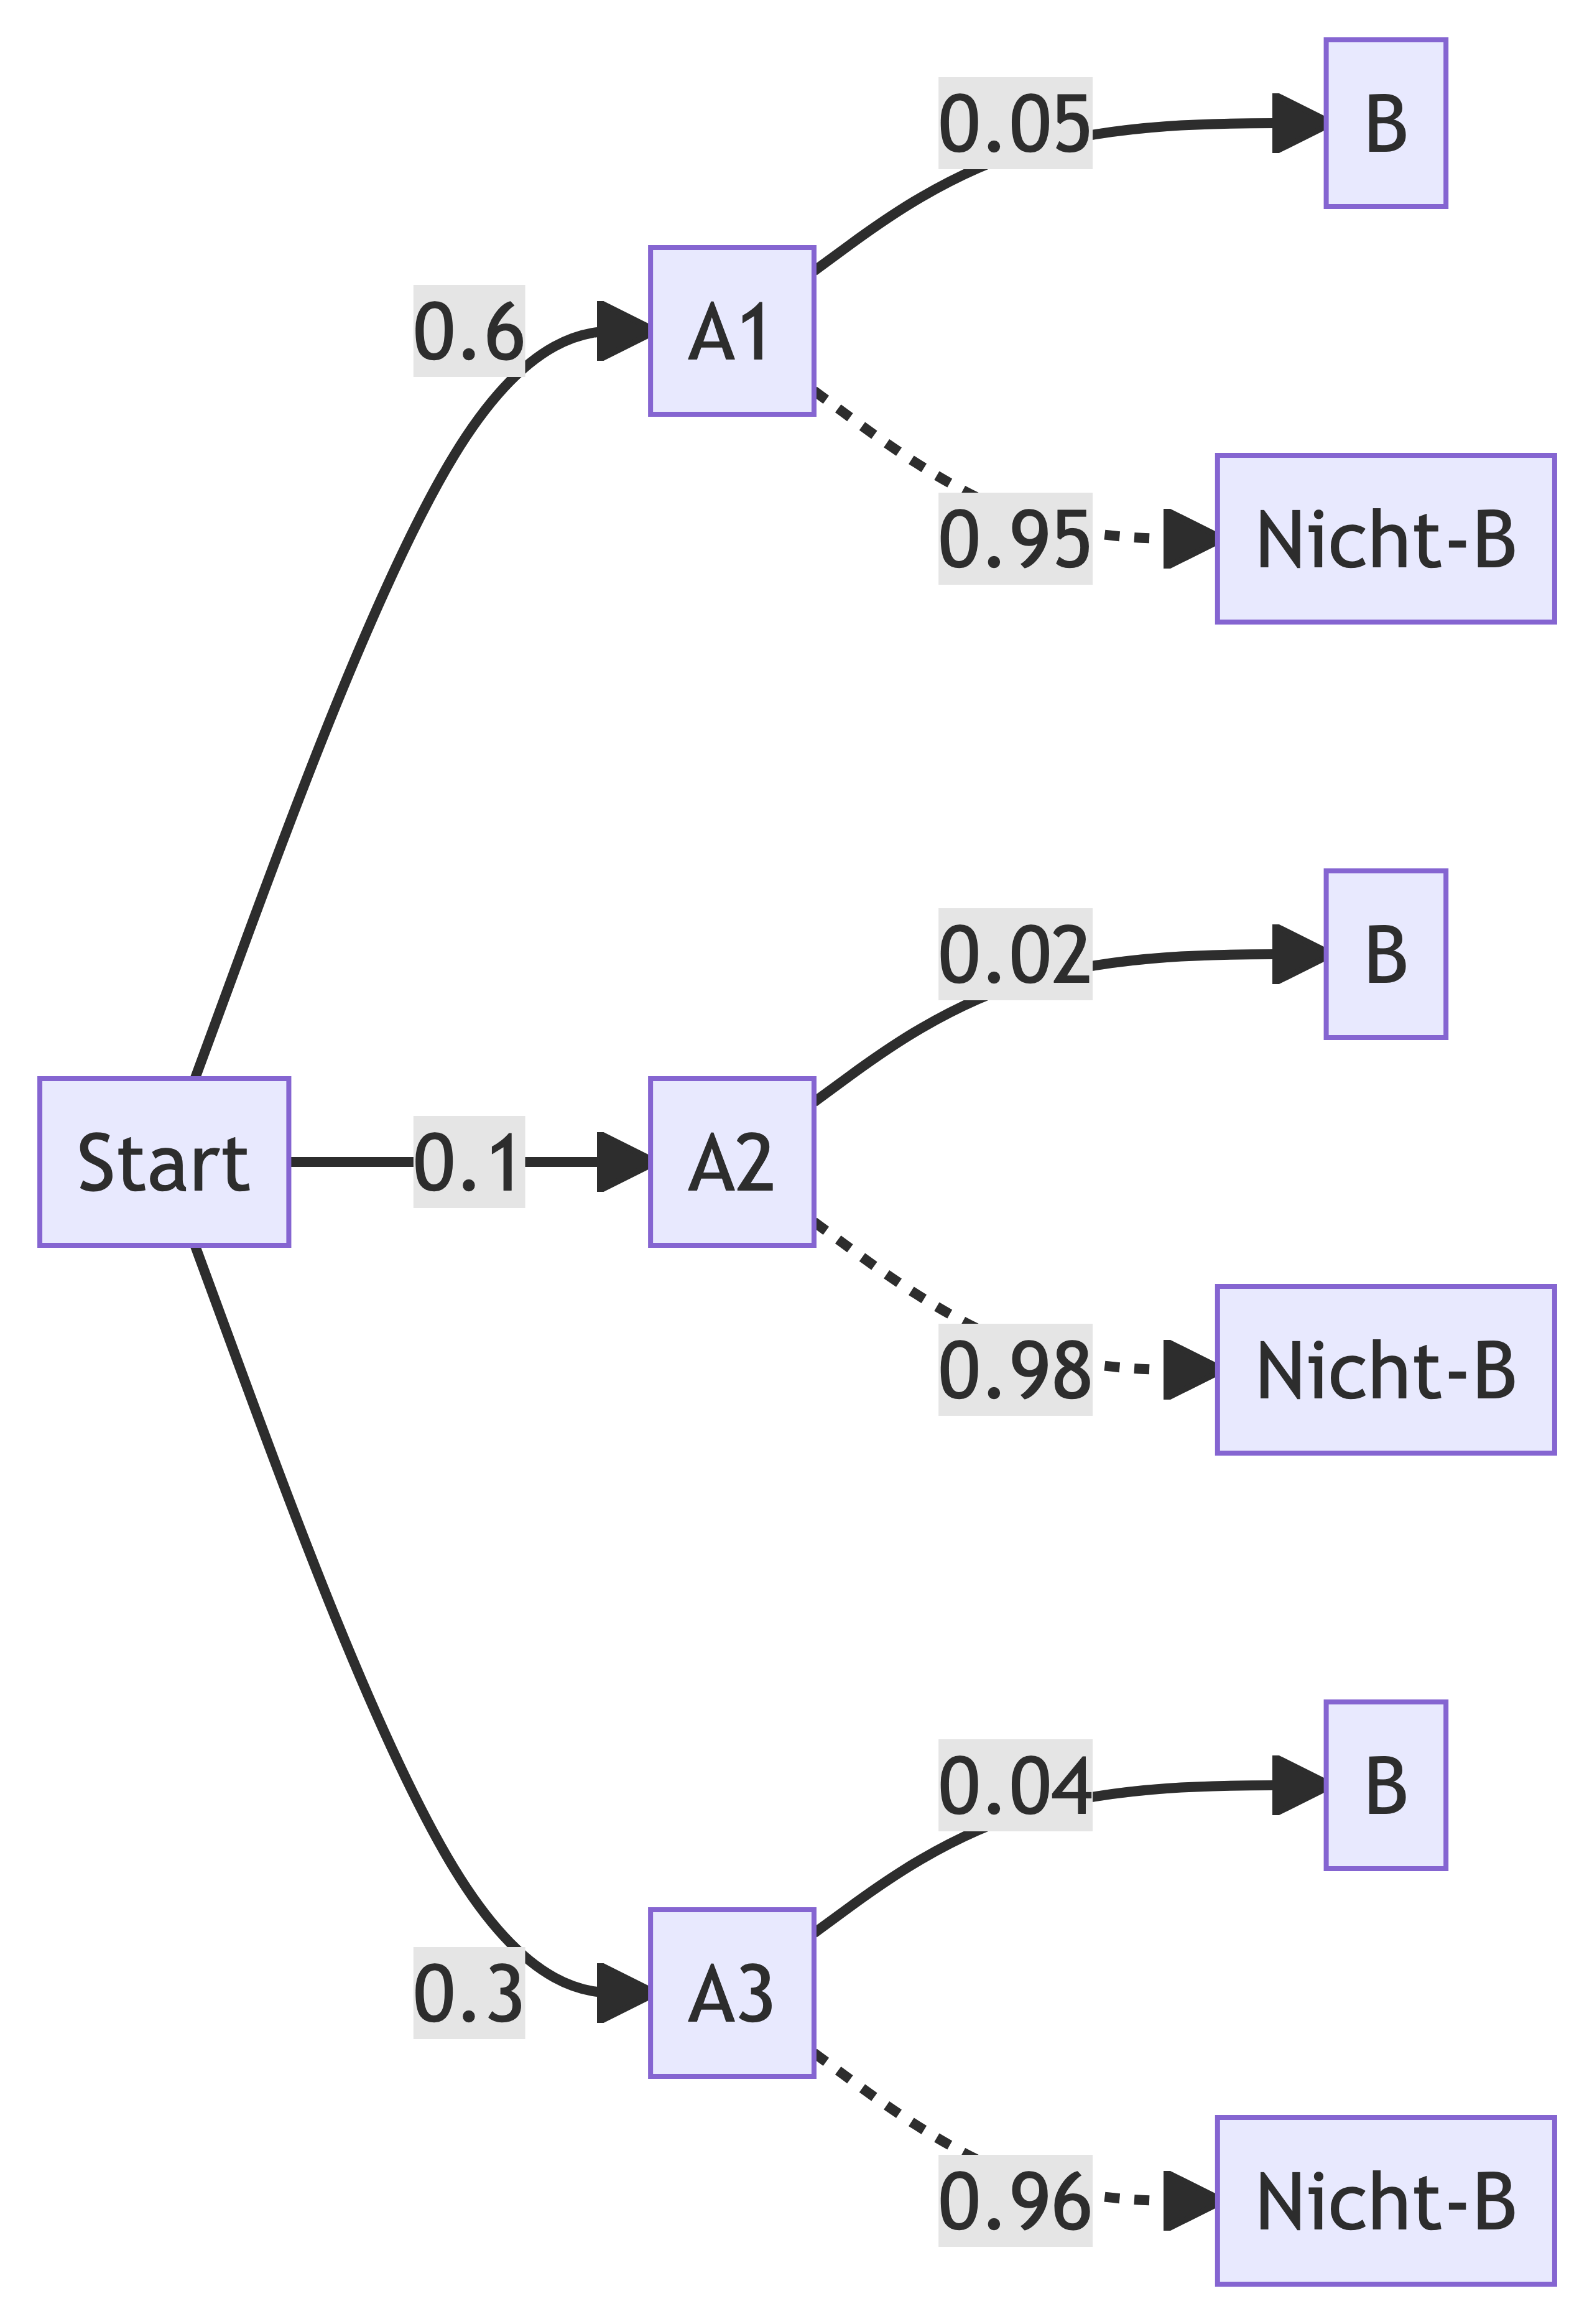
\includegraphics[width=3.34in,height=4.86in]{./Wskt_files/figure-latex/mermaid-figure-3.png}

}

\end{figure}

}

\caption{\label{fig-tot-wskt}Totale Wahrscheinlichkeit}

\end{figure}

Gesucht ist die Wahrscheinlichkeit \(P(B)\).

Dazu addieren wir die Warhscheinlichkeiten der relevanten Äste.

\begin{Shaded}
\begin{Highlighting}[]
\NormalTok{W\_total }\OtherTok{\textless{}{-}} \FloatTok{0.6} \SpecialCharTok{*} \FloatTok{0.05} \SpecialCharTok{+} \FloatTok{0.1} \SpecialCharTok{*} \FloatTok{0.02} \SpecialCharTok{+} \FloatTok{0.3} \SpecialCharTok{*} \FloatTok{0.04}
\NormalTok{W\_total}
\DocumentationTok{\#\# [1] 0.044}
\end{Highlighting}
\end{Shaded}

Die totale Wahrscheinlichkeit beträgt also \(P(B) = 4.4\%\).

Einfacher noch ist es, wenn man anstelle von Wahrscheinlichkeiten
absolute Häufigkeiten verwendet.

\hypertarget{bayes}{%
\subsection{Bayes}\label{bayes}}

\hypertarget{bayes-als-baum}{%
\subsubsection{Bayes als Baum}\label{bayes-als-baum}}

Gesucht sei \(P(A_1|B)\).

Für Bayes' Formel setzt man die Wahrscheinlichkeit des \emph{günstigen}
Ast zur Wahrscheinlichkeit aller relevanten Äste, \(P(B)\).

Der günstige Ast ist hier schwarz gedruckt, die übrigen Äste
gestrichelt, s. Abbildung~\ref{fig-tot-wskt2}.

\begin{figure}

{\centering 

\begin{figure}[H]

{\centering 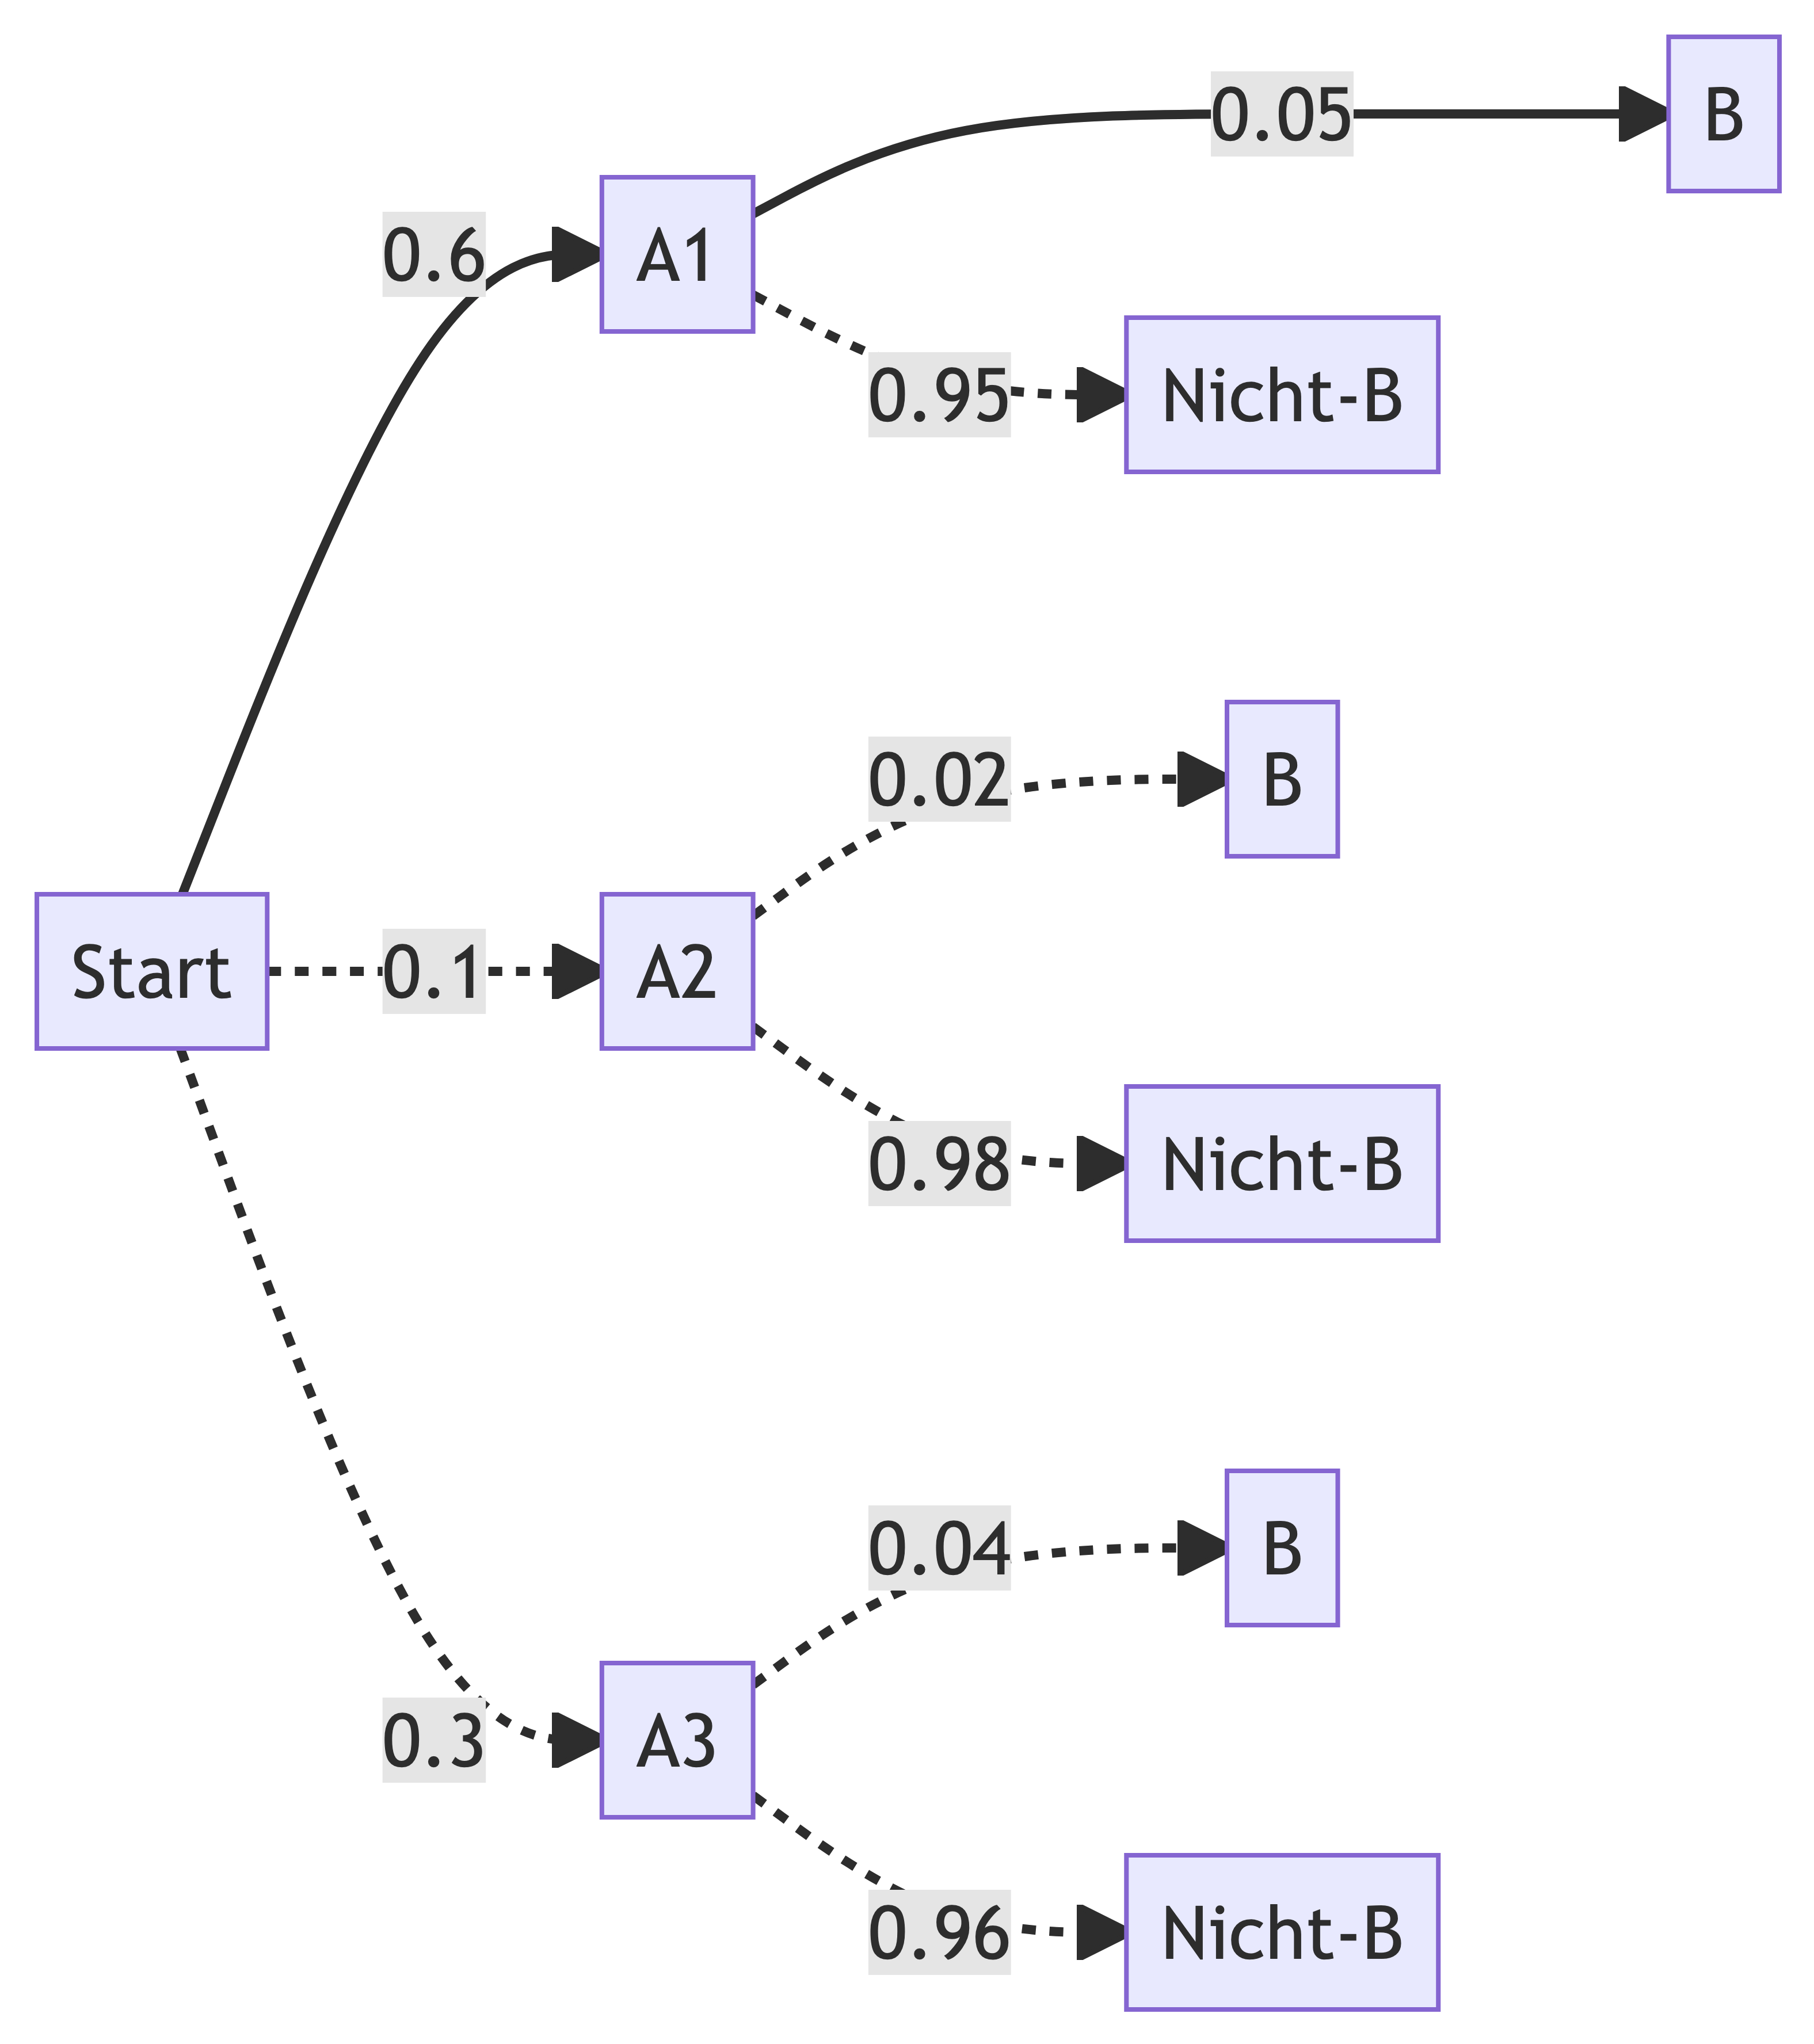
\includegraphics[width=4.11in,height=4.63in]{./Wskt_files/figure-latex/mermaid-figure-2.png}

}

\end{figure}

}

\caption{\label{fig-tot-wskt2}Günstige Pfade}

\end{figure}

\[P(A|B) = \frac{P(A1 \cap B)}{P(B)} = \frac{0.6 \cdot 0.05}{0.03 + 0.002 + 0.012} = \frac{0.03}{0.044} \approx 0.68\]

\(P(A|B)\) beträgt also ca. 68\%.

Zur Erinnerung: \(P(B)\) ist die totale Wahrscheinlichkeit.

\hypertarget{bayes-theorem}{%
\section{Bayes' Theorem}\label{bayes-theorem}}

\hypertarget{bayes-als-bedingte-wahrscheinlichkeit}{%
\subsection{Bayes als bedingte
Wahrscheinlichkeit}\label{bayes-als-bedingte-wahrscheinlichkeit}}

Bayes' Theorem ist auch nur eine normale bedingte Wahrscheinlichkeit:

\(P(A|B) = \frac{\overbrace{ P(A\cap B)}^\text{umformen}}{P(B)}\)

\(P(A\cap B)\) kann man umformen, s. Gleichung~\ref{eq-bayes1}:

\begin{equation}\protect\hypertarget{eq-bayes1}{}{P(A|B) =\frac{P(A\cap B)}{P(B)} = \frac{P(B|A) \cdot P(A)}{P(B)}}\label{eq-bayes1}\end{equation}

Man kann sich Bayes' Theorem auch wie folgt herleiten:

\(P(A\cap B) = P(B \cap A) = P(A) \cdot P(B|A) = P(B) \cdot P(A|B)\)

Dann lösen wir nach P\((A|B)\) auf:

\(P(A|B) = \frac{P(A) \cdot P(B|A)}{P(B)}\)

\hypertarget{wozu-wird-bayes-in-der-praxis-genutzt}{%
\subsection{Wozu wird Bayes in der Praxis
genutzt?}\label{wozu-wird-bayes-in-der-praxis-genutzt}}

In der Praxis nutzt man Bayes häufig, wenn man Daten zu einer Wirkung
\(W\) hat, und auf die Ursache \(U\) zurückschließen möchte, sinngemäß:

\(W \quad \underrightarrow{Bayes} \quad U\).

Dann kann man Gleichung~\ref{eq-bayes1} so schreiben, s.
Gleichung~\ref{eq-bayes2}:

\begin{equation}\protect\hypertarget{eq-bayes2}{}{P(U|W) = \frac{ P(U) \cdot P(W|U) }{P(W)}}\label{eq-bayes2}\end{equation}

Eine ähnliche Situation, die in der Praxis häufig ist, dass man Daten
\(D\) hat und auf die Wahrscheinlichkeit einer Hypothese \(H\) schließen
möchte, s. Gleichung~\ref{eq-bayes3}.

\(D \quad \underrightarrow{Bayes} \quad H\).

\begin{equation}\protect\hypertarget{eq-bayes3}{}{P(H|D) = \frac{ P(H) \cdot P(D|H) }{P(D)}}\label{eq-bayes3}\end{equation}

Gleichung~\ref{eq-bayes3} fragt nach \(P(H|D)\):

\begin{quote}
Was ist die Wahrscheinlichkeit der Hypothese H, jetzt wo wir die Daten
haben (und ein Modell?)
\end{quote}

Und antwortet so (Gleichung~\ref{eq-bayes3}):

\begin{quote}
Diese Wahrscheinlichkeit entspricht der Grundrate
(Apriori-Wahrscheinlichkeit) der Hypothese mal der Plausibilität
(Likelihood) der Daten unter Annahme (gegeben) der Hypothese. Aus
Standardisierungsgründen dividiert man noch die totale
Wahrscheinlichkeit der Daten über alle Hypothesen.
\end{quote}

\hypertarget{zusammengesetzte-hypothesen}{%
\subsection{Zusammengesetzte
Hypothesen}\label{zusammengesetzte-hypothesen}}

Das ist vielleicht ein bisschen fancy, aber man kann Bayes' Theorem auch
nutzen, um die Wahrscheinlichkeit einer \emph{zusammengesetzten
Hypothese} zu berechnen: \(H = H_1 \cap H_2\). Ein Beispiel wäre: ``Was
ist die Wahrscheinlichkeit, dass es Regen (\(R\)) \emph{und} Blitzeis
(\(B\)) gibt, wenn es kalt (\(K\)) ist?''.

Das sieht dann so aus, Gleichung~\ref{eq-bayes4}:

\begin{equation}\protect\hypertarget{eq-bayes4}{}{
\begin{aligned}
P(R \cap B |K) &= \frac{ P(R \cap B) \cdot P(K|R \cap B) }{P(D)} \\
&= \frac{ P(R ) \cdot P(B) \cdot P(K|R \cap B) }{P(D)}
\end{aligned}
}\label{eq-bayes4}\end{equation}

Hier haben wir \(P(R \cap B)\) aufgelöst in \(P(R) \cdot P(B)\), das ist
nur zulässig, wenn \(R\) und \(B\) unabhängig sind.

\hypertarget{bayes-video-von-3b1b}{%
\subsubsection{Bayes-Video von 3b1b}\label{bayes-video-von-3b1b}}

Das \href{https://youtu.be/HZGCoVF3YvM}{Video zu Bayes von 3b1b}
verdeutlicht das Vorgehen der Bayes-Methode auf einfache und
anschauliche Weise.

\hypertarget{aufgaben-1}{%
\section{Aufgaben}\label{aufgaben-1}}

Zusätzlich zu den Aufgaben im Buch:

\begin{itemize}
\tightlist
\item
  \href{https://datenwerk.netlify.app/posts/mtcars-abhaengig/mtcars-abhaengig.html}{mtcars-abhaengig}
\item
  \href{https://datenwerk.netlify.app/posts/voll-normal/voll-normal.html}{voll-normal}
\item
  \href{https://datenwerk.netlify.app/posts/corona-blutgruppe/corona-blutgruppe.html}{corona-blutgruppe}
\item
  \href{https://datenwerk.netlify.app/posts/bed-wskt2/bed-wskt2}{Bed-Wskt2}
\item
  \href{https://datenwerk.netlify.app/posts/gem-wskt1/gem-wskt1}{Gem-Wskt1}
\item
  \href{https://datenwerk.netlify.app/posts/wuerfel01/wuerfel01.html}{wuerfel01}
\item
  \href{https://datenwerk.netlify.app/posts/wuerfel02/wuerfel02.html}{wuerfel02}
\item
  \href{https://datenwerk.netlify.app/posts/wuerfel03/wuerfel03.html}{wuerfel03}
\item
  \href{https://datenwerk.netlify.app/posts/wuerfel04/wuerfel04.html}{wuerfel04}
\end{itemize}

\hypertarget{section-2}{%
\section{---}\label{section-2}}

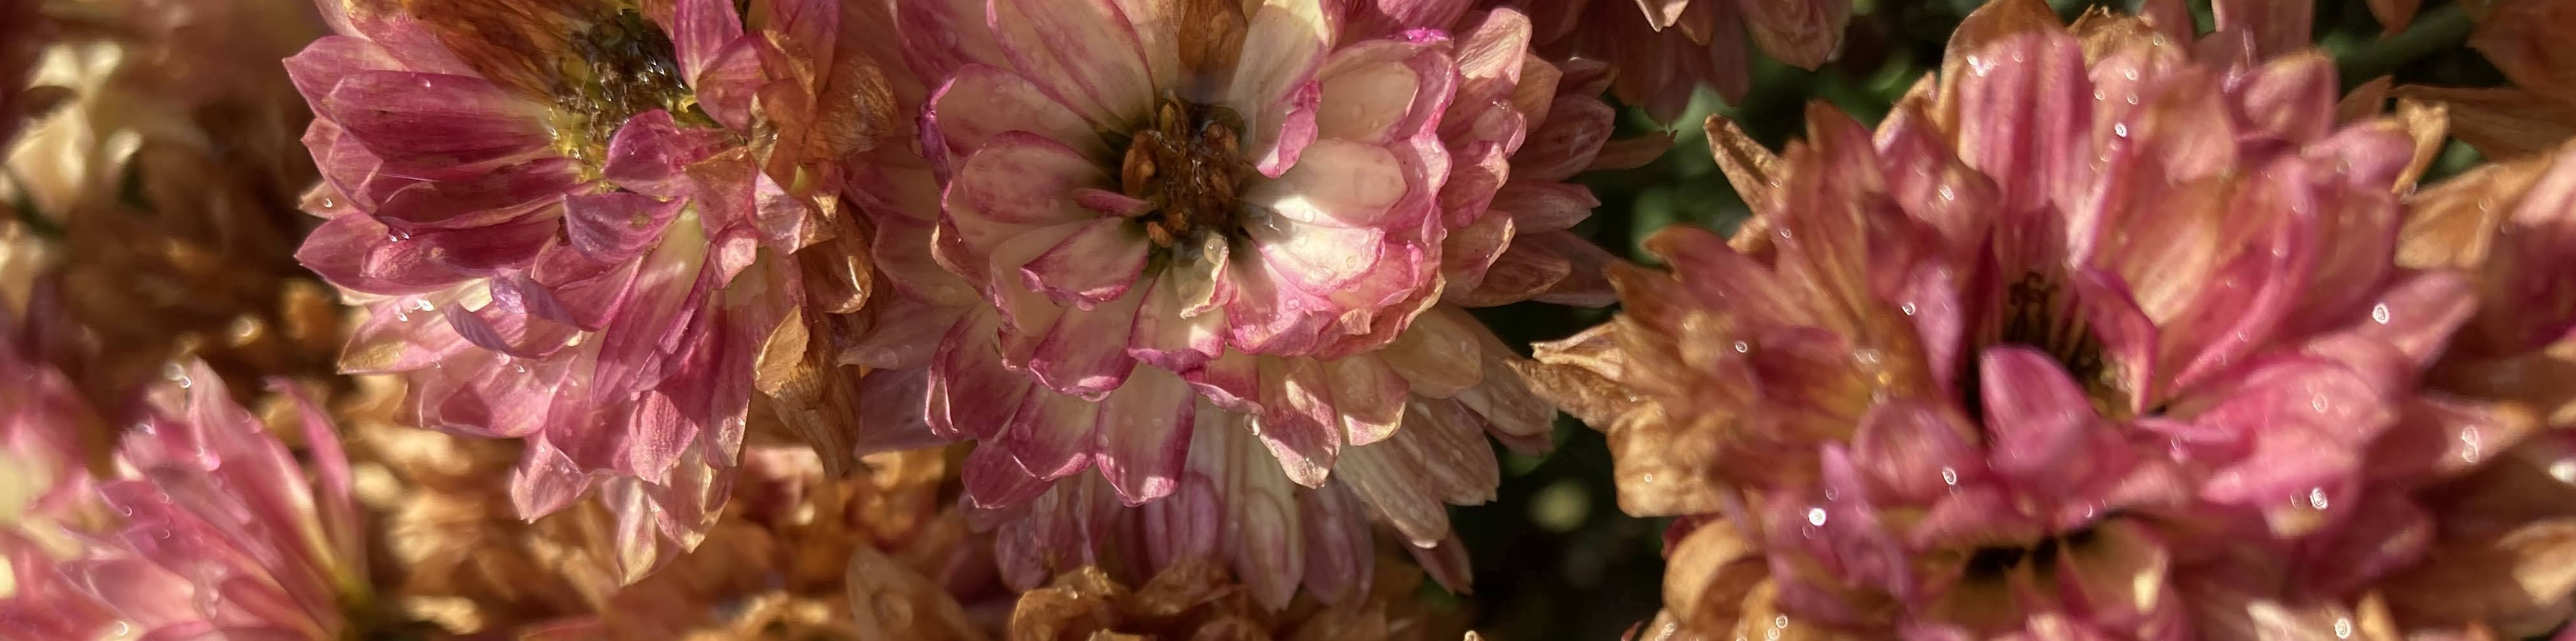
\includegraphics[width=1\textwidth,height=\textheight]{./img/outro-03.jpg}

\bookmarksetup{startatroot}

\hypertarget{verteilungen}{%
\chapter{Verteilungen}\label{verteilungen}}

\hypertarget{lernsteuerung-2}{%
\section{Lernsteuerung}\label{lernsteuerung-2}}

\hypertarget{lernziele-3}{%
\subsection{Lernziele}\label{lernziele-3}}

Nach Absolvieren des jeweiligen Kapitels sollen folgende Lernziele
erreicht sein.

Sie können \ldots{}

\begin{itemize}
\tightlist
\item
  den Begriff der Zufallsvariablen erläutern
\item
  die Begriffe von Wahrscheinlichkeitsdichte und Verteilungsfunktion
  erläutern und anhand einfacher Beispiele ausrechnen
\item
  den Begriff einer Gleichverteilung erläutern und einfache
  Fallbeispiele ausrechnen
\item
  die Parameter einer Normalverteilung nennen und erläutern
\end{itemize}

\hypertarget{pruxfcfungsrelevanter-stoff-1}{%
\subsection{Prüfungsrelevanter
Stoff}\label{pruxfcfungsrelevanter-stoff-1}}

Lesen Sie zusätzlich zum Stoff dieses Kapitels noch Bourier (2018),
folgende Abschnitte:

\begin{itemize}
\tightlist
\item
  Kap. 6.1 (Zum Begriff Zufallsvariable)
\item
  Kap. 6.3 (Stetige Zufallsvariablen)
\item
  Kap. 7.1.1 (Binomialverteilung)
\item
  Kap. 7.2.1 (Gleichverteilung) und 7.2.3 (Normalverteilung)
\end{itemize}

Lösen Sie auch die Übungsaufgaben dazu.

Weitere Übungsaufgaben finden Sie im dazugehörigen Übungsbuch, Bourier
(2022).

\hypertarget{benuxf6tigte-r-pakete}{%
\subsection{Benötigte R-Pakete}\label{benuxf6tigte-r-pakete}}

\begin{Shaded}
\begin{Highlighting}[]
\FunctionTok{library}\NormalTok{(patchwork)}
\FunctionTok{library}\NormalTok{(tidyverse)}
\end{Highlighting}
\end{Shaded}

\hypertarget{zentrale-begriffe-1}{%
\subsection{Zentrale Begriffe}\label{zentrale-begriffe-1}}

\hypertarget{eigenschaften-von-zufallsvariablen}{%
\subsubsection{Eigenschaften von
Zufallsvariablen}\label{eigenschaften-von-zufallsvariablen}}

\begin{itemize}
\tightlist
\item
  Zufallsvariable (random variable)
\item
  Diskret vs.~stetig
\item
  Wahrscheinlichkeitsdichte (Dichte, (probability) density, f)
\item
  Wahrscheinlichkeitsfunktion (kumulierte Wahrscheinlichkeit,
  Wahrscheinlichkeitsmasse)
\end{itemize}

\hypertarget{verteilungen-1}{%
\subsubsection{Verteilungen}\label{verteilungen-1}}

\begin{itemize}
\tightlist
\item
  Gleichverteilung
\item
  Normalverteilung
\item
  Standardnormalverteilung
\end{itemize}

\hypertarget{begleitvideos-2}{%
\subsection{Begleitvideos}\label{begleitvideos-2}}

\begin{itemize}
\tightlist
\item
  \href{https://youtu.be/7GqIE4sKDs4}{Video 1 zum Thema Verteilungen}
\item
  \href{https://youtu.be/HKWwondYsW8}{Video 2 zum Thema Verteilungen}
\end{itemize}

\hypertarget{verteilungen-2}{%
\section{Verteilungen}\label{verteilungen-2}}

\begin{tcolorbox}[enhanced jigsaw, colframe=quarto-callout-important-color-frame, breakable, titlerule=0mm, left=2mm, colbacktitle=quarto-callout-important-color!10!white, opacityback=0, colback=white, opacitybacktitle=0.6, toptitle=1mm, rightrule=.15mm, toprule=.15mm, bottomrule=.15mm, bottomtitle=1mm, title=\textcolor{quarto-callout-important-color}{\faExclamation}\hspace{0.5em}{Wichtig}, leftrule=.75mm, arc=.35mm, coltitle=black]

Eine \emph{Verteilung} zeigt, welche Ausprägungen eine Variable aufweist
und wie häufig bzw. wahrscheinlich diese sind. Einfach gesprochen,
veranschaulicht eine Balken- oder Histogramm eine Verteilung. Man
unterscheidet Häufigkeitsverteilungen (s. Abb.
Abbildung~\ref{fig-mtcars-freq}) von Wahrscheinlichkeitsverteilungen
(Abb. Abbildung~\ref{fig-uniform}).

\end{tcolorbox}

\hypertarget{huxe4ufigkeitsverteilung}{%
\subsection{Häufigkeitsverteilung}\label{huxe4ufigkeitsverteilung}}

Die Häufigkeitsverteilung eines \emph{diskreten} Merkmals \(X\) mit
\(k\) Ausprägungen zeigt, wie häufig die einzelnen Ausprägungen sind. So
hat die Variable \emph{Zylinder} (in einem Datensatz) etwa die
Ausprägungen 4,6 und 8.

\begin{Shaded}
\begin{Highlighting}[]
\FunctionTok{data}\NormalTok{(mtcars)}
\NormalTok{  mtcars }\SpecialCharTok{\%\textgreater{}\%} 
    \FunctionTok{count}\NormalTok{(cyl)}
\end{Highlighting}
\end{Shaded}

\begin{longtable}[]{@{}rr@{}}
\toprule()
cyl & n \\
\midrule()
\endhead
4 & 11 \\
6 & 7 \\
8 & 14 \\
\bottomrule()
\end{longtable}

Abb. Abbildung~\ref{fig-mtcars-freq}, links, visualisiert die
Häufigkeitsverteilung von \texttt{cyl}.

\begin{figure}

{\centering 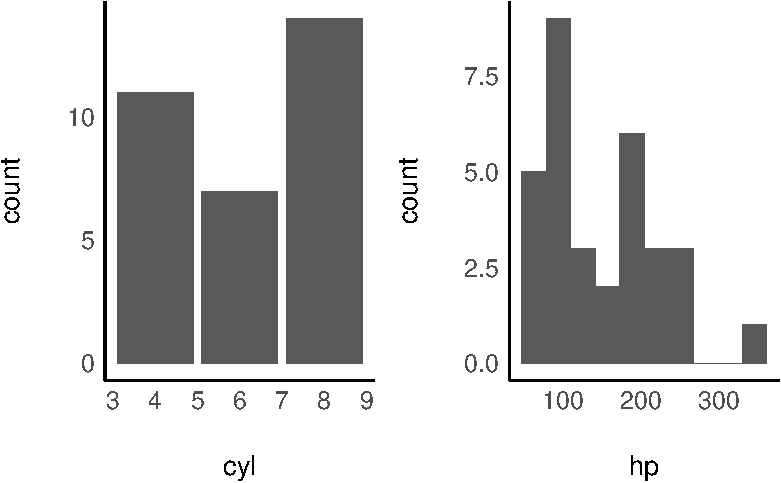
\includegraphics{./Verteilungen_files/figure-pdf/fig-mtcars-freq-1.pdf}

}

\caption{\label{fig-mtcars-freq}Häufigkeitsverteilung von \texttt{cyl}
und \texttt{hp} (diskretisiert in 10 Körbe oder Gruppen)}

\end{figure}

Ein \emph{stetiges} Merkmal, wie \texttt{hp} (PS-Zahl), lässt sich durch
Klassenbildung in ein diskretes umwandeln (diskretisieren), s. Abb.
Abbildung~\ref{fig-mtcars-freq}, rechts.

\hypertarget{wahrscheinlichkeitsverteilung}{%
\subsection{Wahrscheinlichkeitsverteilung}\label{wahrscheinlichkeitsverteilung}}

Wahrscheinlichkeitsverteilungen dienen dazu, Ereignissen einer
Zufallsvariable eine Wahrscheinlichkeit zuzuordnen.

Eine \emph{diskrete} Wahrscheinlichkeitsverteilung der (diskreten)
Zufallsvariablen \(X\) ordnet jeder der \(k\) Ausprägungen \(X=x\) eine
Wahrscheinlichkeit \(p\) zu. So hat die Variable \emph{Geschlecht eines
Babies} die beiden Ausprägungen \emph{Mädchen} und \emph{Junge} mit den
Wahrscheinlichkeiten \(p_M = 51.2\%\) bzw. \(p_J = 48.8\%\) (Gelman,
Hill, und Vehtari 2021).

Bei \emph{stetigen} Zufallsvarialben \(X\) geht man von unendlich vielen
Ausprägungen aus; die Wahrscheinlichkeit einer bestimmten Ausprägung ist
(praktisch) Null: \(p(X=x_j)=0, \quad j=1,...,+\infty\). So ist die
Wahrscheinlichkeit, dass eine Person exakt 166,66666666\ldots{} cm groß
ist, (praktisch) Null. Man gibt stattdessen die \emph{Dichte} der
Wahrscheinlichkeit an: Das ist die Wahrscheinlichkeit(smasse) pro
Einheit von \(X\).

\hypertarget{gleichverteilung}{%
\section{Gleichverteilung}\label{gleichverteilung}}

\hypertarget{indifferenz-als-grundlage}{%
\subsection{Indifferenz als Grundlage}\label{indifferenz-als-grundlage}}

Eine Gleichverteilung nimmt an, dass jeder Wert im Ergebnisraum der
zugehörigen Zufallsvariable \emph{gleichwahrscheinlich} ist. Wenn man
keinen hinreichenden Grund hat, eine Realisation einer Zufallsvariablen
für plausibler als einen anderen zu halten, ist eine Gleichverteilung
eine passende Verteilung. Gleichverteilungen gibt es im diskreten und im
stetigen Fall.

Abb. Abbildung~\ref{fig-uniform} zeigt ein Beispiel für eine (stetige)
Gleichverteilung.

\begin{figure}

{\centering 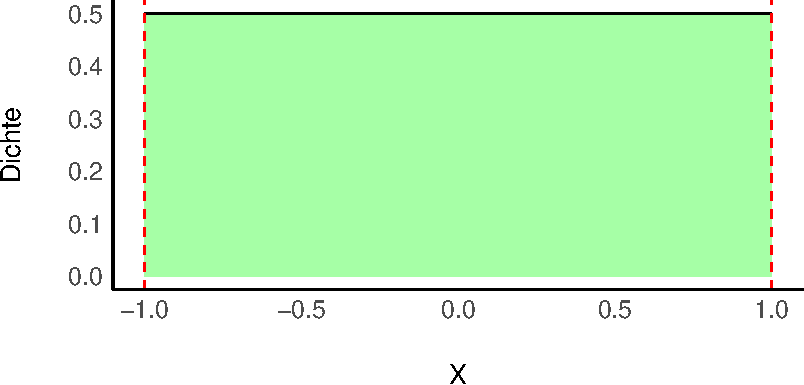
\includegraphics{./Verteilungen_files/figure-pdf/fig-uniform-1.pdf}

}

\caption{\label{fig-uniform}Gleichverteilung min=-1, max=1}

\end{figure}

Bei \(X=0\) hat eine Einheit von \(X\) die Wahrscheinlichkeitsmasse von
50\%.

Definierendes Kennzeichen einer Gleichverteilung ist die \emph{konstante
Dichte}.

\hypertarget{simulation}{%
\subsection{Simulation}\label{simulation}}

Möchte man die Verteilungsfunktion einer stetigen Zufallsvariablen
berechnen, kann das ganz schön kompliziert werden, schließlich muss man
Integrale lösen. Aber es gibt einen Trick, wie man die Sache stark
vereinfachen kann: man simuliert die Verteilung. Was bedeutet das?

Angenommen, die Wartezeit auf einen Bus ist gleichverteilt (engl.
\emph{uniform distribution}); der Bus kommt regelmäßig und püunktlich
alle 10 Minuten. Die minimale Wartezeit beträgt also 0 Minuten und die
maximale 10 Minuten. Nennen wir die zugehörige Zufallsvariable \(X\),
das ist schön kurz.

Dann schreibt man auch:

\[X \sim Unif(0,10).\]

Ja, das sieht fancy aus, aber wo ist der versprochene Trick zum
Vereinfachen? Kommt gleich, Moment.

Eine Frage könnte nun lauten, wie groß ist die Wahrscheinlichkeit, dass
man zwischen 3 und 5 Minuten auf den Bus warten muss?

Der Trick ist, dass wir Integralrechnung gegen stumpfes Zählen
eintauschen.

Computer (und damit R) haben eingebaut Funktionen, die eine beliebige
Zufallszahl ziehen können, zum Beispiel gleichverteilt

Auf Errisch heißt das Zauberwort \texttt{runif()}:

\begin{Shaded}
\begin{Highlighting}[]
\FunctionTok{runif}\NormalTok{(}\AttributeTok{n =} \DecValTok{1}\NormalTok{, }\AttributeTok{min =} \DecValTok{0}\NormalTok{, }\AttributeTok{max =} \DecValTok{10}\NormalTok{)}
\end{Highlighting}
\end{Shaded}

\begin{verbatim}
## [1] 9.14806
\end{verbatim}

Auf Deutsch heißt das: ``Hey R, ich hätte gerne eine (daher
\texttt{n\ =\ 1}) Zufallszahl \emph{r} wie \emph{random}, die
gleichverteilt ist (\emph{uniform}) mit \texttt{min\ =\ 0} und
\texttt{max\ =\ 10}.

(Zu) anschaulich gesprochen: R hat den Bus kommen lassen und es hat gut
9.1 Minuten gedauert, bis er da war.

Achtung, jetzt kommt's: Jetzt lassen wir R mal \(10^5\) (\texttt{1e5}
auf Computersprech) Busse vorfahren. R soll jedes Mal notieren, wie
lange man auf den Bus warten musste.\footnote{Machen Sie das mal ohne
  Computer, wenn Sie ein Wochenende Langeweile haben.}

\begin{Shaded}
\begin{Highlighting}[]
\NormalTok{x\_simu }\OtherTok{\textless{}{-}} \FunctionTok{runif}\NormalTok{(}\AttributeTok{n =} \FloatTok{1e5}\NormalTok{, }\AttributeTok{min =} \DecValTok{0}\NormalTok{, }\AttributeTok{max =} \DecValTok{10}\NormalTok{)}
\end{Highlighting}
\end{Shaded}

Schauen wir uns die Verteilung an, Abbildung~\ref{fig-simu-gleichvert}.

\begin{Shaded}
\begin{Highlighting}[]
\FunctionTok{ggplot}\NormalTok{(x\_simu\_df) }\SpecialCharTok{+}
  \FunctionTok{aes}\NormalTok{(}\AttributeTok{x =}\NormalTok{ x\_simu) }\SpecialCharTok{+}
  \FunctionTok{geom\_histogram}\NormalTok{(}\AttributeTok{bins =} \DecValTok{50}\NormalTok{)}
\end{Highlighting}
\end{Shaded}

\begin{figure}[H]

{\centering 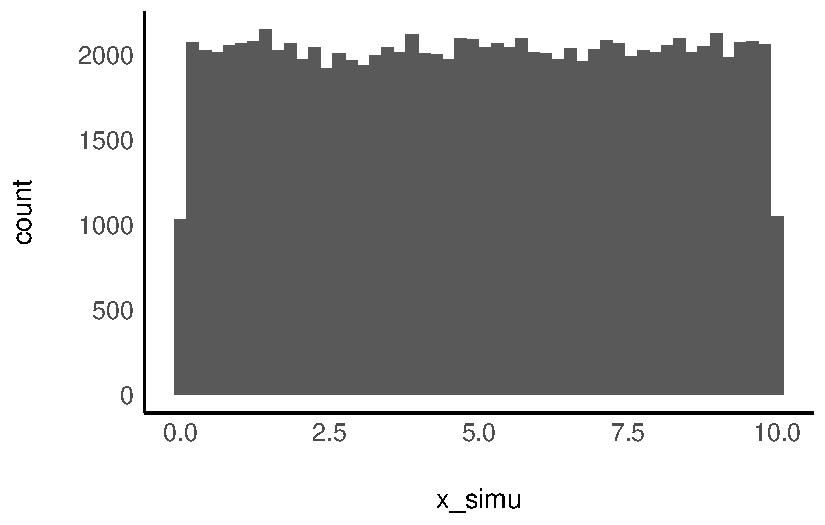
\includegraphics{./Verteilungen_files/figure-pdf/fig-simu-gleichvert-1.pdf}

}

\caption{\label{fig-simu-gleichvert}Simulation einer gleichverteiluten
Zufallsvariablen}

\end{figure}

Okay, unsere Verteilung sieht nicht \emph{exakt} gleichverteilt, aber
einigermaßen. Gut genug für unsere Zwecke!

So, und jetzt kommt das Ernten. Wir können jetzt nämlich einfach zählen
(\texttt{count()}), um die Antwort auf unsere Frage (der Wartezeit 3-5
Min.) zu erhalten.

\begin{Shaded}
\begin{Highlighting}[]
\NormalTok{x\_simu\_df }\SpecialCharTok{\%\textgreater{}\%} 
  \FunctionTok{count}\NormalTok{(}\AttributeTok{Schnittmenge =}\NormalTok{ x }\SpecialCharTok{\textgreater{}} \DecValTok{3} \SpecialCharTok{\&}\NormalTok{ x }\SpecialCharTok{\textless{}} \DecValTok{5}\NormalTok{)}
\end{Highlighting}
\end{Shaded}

\begin{longtable}[]{@{}lr@{}}
\toprule()
Schnittmenge & n \\
\midrule()
\endhead
FALSE & 80072 \\
TRUE & 19928 \\
\bottomrule()
\end{longtable}

Das Zeichen \texttt{\&} ist das logische UND, also die Schnittmenge der
zwei Mengen \(A := \{x|x>3\}\) und \(B := \{x|x<5\}\), also
\(A \cap B\).

Wie man sieht, fallen ca. 20\% der Stichproben in den entsprechenden
Bereich.

Da viele Probleme, wenn sie komplexer werden, kaum noch analytisch (wie
Integrieren) ausrechenbar sind, greift man in der modernen
(Analyse-)Welt oft lieber auf Simulationsverfahren zurück - Dank sei den
schnellen Rechnern. Für uns Menschen ist damit die Aufgabe des
Integrierens auf schnödes Zählen zurückgeführt.

\hypertarget{sec-bin-distrib}{%
\section{Binomialverteilung}\label{sec-bin-distrib}}

\begin{tcolorbox}[enhanced jigsaw, colframe=quarto-callout-important-color-frame, breakable, titlerule=0mm, left=2mm, colbacktitle=quarto-callout-important-color!10!white, opacityback=0, colback=white, opacitybacktitle=0.6, toptitle=1mm, rightrule=.15mm, toprule=.15mm, bottomrule=.15mm, bottomtitle=1mm, title=\textcolor{quarto-callout-important-color}{\faExclamation}\hspace{0.5em}{Wichtig}, leftrule=.75mm, arc=.35mm, coltitle=black]

Die Binomialverteilung dient zur Darstellung der Wahrscheinlichkeit der
Ergebnisse eines wiederholten binomialen Zufallexperiments, eines
Zufallsexperiments mit \emph{zwei} Ergebnissen also. Typisches Beispiel
ist ein Münzwurf. Bei jeder Wiederholung des Zufallexperiments bleibt
die Wahrscheinlichkeit der Ergebnisse gleich: Die Münze verändert sich
nicht durch die Würfe (Ziehen mit Zurücklegen). Außerdem hat ein
bestimmtes Ergebnis im ersten Wurf keinen Einfluss auf die
Wahrscheinlichkeit eines bestimmten Ergebnisses im zweiten Wurf, etc.

\end{tcolorbox}

\hypertarget{veranschaulichung}{%
\subsection{Veranschaulichung}\label{veranschaulichung}}

Stellen wir uns eine Kistchen\footnote{In den Lehrbüchern häufig als
  Urne bezeichnet, was den bösen Spott von ``Friedhofstatistik'' nach
  sich zog.} mit 5 Losen vor, darunter 2 \emph{T}reffer (Gewinn) und 3
\emph{N}ieten, s. Abb. Abbildung~\ref{fig-urne}. Der Versuch läuft so
ab: Wir ziehen ein Los, schauen ob es ein Treffer ist oder nicht, legen
es zurück und ziehen erneut.

\begin{figure}

{\centering 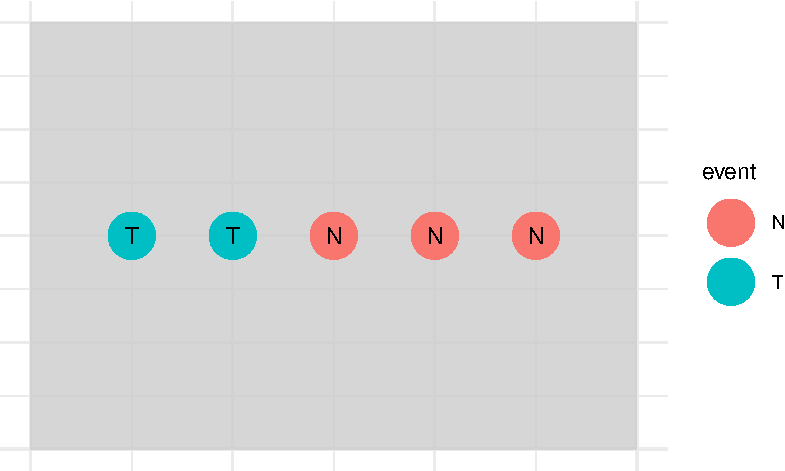
\includegraphics{./Verteilungen_files/figure-pdf/fig-urne-1.pdf}

}

\caption{\label{fig-urne}Ein Kästchen mit 5 Losen, darunter 2 Treffer
und 3 Nieten.}

\end{figure}

\begin{tcolorbox}[enhanced jigsaw, colframe=quarto-callout-important-color-frame, breakable, titlerule=0mm, left=2mm, colbacktitle=quarto-callout-important-color!10!white, opacityback=0, colback=white, opacitybacktitle=0.6, toptitle=1mm, rightrule=.15mm, toprule=.15mm, bottomrule=.15mm, bottomtitle=1mm, title=\textcolor{quarto-callout-important-color}{\faExclamation}\hspace{0.5em}{Wichtig}, leftrule=.75mm, arc=.35mm, coltitle=black]

Um die Wahrscheinlichkeitsverteilung einer binomialverteilte
Zufallsvariable ausrechnen zu können, muss man zwei Dinge wissen:
Erstens die Anzahl der Züge, \(n\) (Stichprobengröße) und zweitens die
Trefferwahrscheinlichkeit, \(p\).

\end{tcolorbox}

Wie groß ist die Wahrscheinlichkeit von \(A^{\prime}\), d.h. bei \(n=4\)
Zügen \(x=2\) Treffer zu erzielen, gegeben dass die
Trefferwahrscheinlichkeit bei \(p=2/4\) liegt?

Wir könnten jetzt ein Baumdiagramm zeichnen und pro Pfad die
Wahrscheinlichkeit ausrechnen (Multiplikationssatz), s.
Abbildung~\ref{fig-3muenzen}. Die Summe der Wahrscheinlichkeiten der
Pfade ist dann die gesuchte Wahrscheinlichkeit, \(W\) (Additionssatz).
Das ist einfach, dauert aber.

In diesem Fall ist die Wahrscheinlichkeit eines (günstigen) Pfades,
\(A\):

\(P(A) = P(T)^2 \cdot P(N)^2 = \left( \frac{2}{5} \right)^2 \cdot \left( \frac{3}{5} \right) ^2\).

\begin{Shaded}
\begin{Highlighting}[]
\NormalTok{p\_a }\OtherTok{=}\NormalTok{ (}\DecValTok{2}\SpecialCharTok{/}\DecValTok{5}\NormalTok{)}\SpecialCharTok{\^{}}\DecValTok{2} \SpecialCharTok{*}\NormalTok{ (}\DecValTok{3}\SpecialCharTok{/}\DecValTok{5}\NormalTok{)}\SpecialCharTok{\^{}}\DecValTok{2}
\NormalTok{p\_a}
\DocumentationTok{\#\# [1] 0.0576}
\end{Highlighting}
\end{Shaded}

Etwas mühevolles Zählen der Pfade würde uns zeigen, dass es \(k=6\)
Pfade gibt, die alle die gleiche Wahrscheinlichkeit, \(P(A)\),
aufweisen.

Damit beträgt die Wahrscheinlichkeit des gesuchten Ereignisses
\(A^{\prime}\) (2 Treffer bei 4 Zügen):

\(P(A^{\prime}) = 6 \cdot P(A)\).

\begin{Shaded}
\begin{Highlighting}[]
\NormalTok{p\_a\_strich }\OtherTok{=} \DecValTok{6} \SpecialCharTok{*}\NormalTok{ p\_a}
\NormalTok{p\_a\_strich}
\DocumentationTok{\#\# [1] 0.3456}
\end{Highlighting}
\end{Shaded}

Mithilfe der Formel der Binomialverteilung lässt sich das Ergebnis, die
Wahrscheinlichkeit von \(A^{\prime}\) schneller ausrechnen. Einfach
gesprochen sieht sie so aus:

\[P(A^{\prime}) = k \cdot P(A)\] Dabei steht \(k\) für die Anzahl der
günstigen Pfade und \(P(A)\) für die Wahrscheinlichkeit eines günstigen
Pfades (d.h. 2 Treffer und 2 Nieten) und alle Pfade haben die gleiche
Wahrscheinlichkeit.

Die Anzahl der Pfade kann man mit dem \emph{Binomialkoeffizient}
ausrechnen, den man so darstellt:

\(\tbinom{n}{k}\)

Lies: ``Wähle aus \(n\) möglichen Ereignissen (Pfade im Baum) \(k\)
günstige Ereignisse (günstige Pfade).

Auf Errisch geht das so:

\begin{Shaded}
\begin{Highlighting}[]
\FunctionTok{choose}\NormalTok{(}\DecValTok{4}\NormalTok{,}\DecValTok{2}\NormalTok{)}
\DocumentationTok{\#\# [1] 6}
\end{Highlighting}
\end{Shaded}

\hypertarget{rechnen-mit-r}{%
\subsection{Rechnen mit R}\label{rechnen-mit-r}}

Die Binomialverteilung ist in R eingebaut; man kann sich leicht
entsprechende Wahrscheinlichkeiten ausrechnen lassen.

Die Wahrscheinlichkeit, bei 4 Zügen 2 Treffer zu erzielen mit \(p=2/5\)
unter der Annahme einer Binomialverteilung lässt sich so mit R
berechnen:

\begin{Shaded}
\begin{Highlighting}[]
\FunctionTok{dbinom}\NormalTok{(}\AttributeTok{x =} \DecValTok{2}\NormalTok{, }\AttributeTok{size =} \DecValTok{4}\NormalTok{, }\AttributeTok{prob =} \DecValTok{2}\SpecialCharTok{/}\DecValTok{5}\NormalTok{)}
\DocumentationTok{\#\# [1] 0.3456}
\end{Highlighting}
\end{Shaded}

\leavevmode\vadjust pre{\hypertarget{exm-binom}{}}%
\begin{example}[Pumpstation-Beispiel zur
Binomialverteilung]\label{exm-binom}

In einer Pumpstation arbeiten 7 Motoren, die wir als identisch annehmen.
Mit einer Wahrscheinlichkeit von 5\% fällt ein Motor aus und ist für den
Rest des Tages nicht einsatzbereit. Der Betrieb kann aufrecht erhalten
werden, solange mindestens 5 Motoren arbeiten. Wie groß ist die
Wahrscheinlichkeit, dass die Pumpstation aus dem Betrieb fällt?

\(P(X=k)\) (oder kurz: \(P(k)\)) gibt die Wahrscheinlichkeit
(Wahrscheinlichkeitsfunktion) an für das Ereignis, dass \emph{k} Motoren
arbeiten.

Lassen wir R mal \(P(X=5)\) ausrechnen.

\begin{Shaded}
\begin{Highlighting}[]
\FunctionTok{dbinom}\NormalTok{(}\AttributeTok{x =} \DecValTok{5}\NormalTok{, }\AttributeTok{size =} \DecValTok{7}\NormalTok{, }\AttributeTok{prob =}\NormalTok{ .}\DecValTok{95}\NormalTok{)}
\DocumentationTok{\#\# [1] 0.0406235}
\end{Highlighting}
\end{Shaded}

Es gilt also \(P(X=5) \approx .04\). Die Wahrscheinlichkeit, dass (nur)
5 Motoren laufen an einem beliebigen Tag ist relativ gering\footnote{wobei
  ``gering'' subjektiv ist, die Betreiberfirma findet diese
  Wahrscheinlichkeit, dass 2 Pumpen ausfallen, wohl viel zu hoch.}.

\texttt{dbinom()} steht für die Wahrscheinlichkeits\emph{d}ichte (im
diskreten Fall, also hier, Wahrscheinlichkeitsfunktion genannt) und
\texttt{binom} für die Binomialverteilung. \texttt{x} gibt die Anzahl
der Treffer an (das gesuchte Ereignis, hier 5 Motoren arbeiten);
\texttt{size} gibt die Stichprobengröße an (hier 7 Motoren).

Damit gilt:

\(P(X\ge 5) = P(X=5) + P(X=6) + P(X=7)\)

\begin{Shaded}
\begin{Highlighting}[]
\NormalTok{p\_5 }\OtherTok{\textless{}{-}} \FunctionTok{dbinom}\NormalTok{(}\AttributeTok{x =} \DecValTok{5}\NormalTok{, }\AttributeTok{size =} \DecValTok{7}\NormalTok{, }\AttributeTok{prob =}\NormalTok{ .}\DecValTok{95}\NormalTok{)}
\NormalTok{p\_6 }\OtherTok{\textless{}{-}} \FunctionTok{dbinom}\NormalTok{(}\AttributeTok{x =} \DecValTok{6}\NormalTok{, }\AttributeTok{size =} \DecValTok{7}\NormalTok{, }\AttributeTok{prob =}\NormalTok{ .}\DecValTok{95}\NormalTok{)}
\NormalTok{p\_7 }\OtherTok{\textless{}{-}} \FunctionTok{dbinom}\NormalTok{(}\AttributeTok{x =} \DecValTok{7}\NormalTok{, }\AttributeTok{size =} \DecValTok{7}\NormalTok{, }\AttributeTok{prob =}\NormalTok{ .}\DecValTok{95}\NormalTok{)}

\NormalTok{p\_mind\_5 }\OtherTok{\textless{}{-}}\NormalTok{ p\_5 }\SpecialCharTok{+}\NormalTok{ p\_6 }\SpecialCharTok{+}\NormalTok{ p\_7}

\NormalTok{p\_mind\_5}
\DocumentationTok{\#\# [1] 0.996243}
\end{Highlighting}
\end{Shaded}

Die Wahrscheinlichkeit, dass mind. 5 Motoren arbeiten beträgt also
0.9962.

Das Komplement zu diesem Ereignis ist, dass \emph{nicht} mind. 5 Motoren
arbeiten, also höchstens 4 und es daher zu einem Ausfall kommt.

Natürlich gilt \(P(\bar{X}) = 1- P(X)\).

\begin{Shaded}
\begin{Highlighting}[]
\NormalTok{p\_weniger\_als\_4 }\OtherTok{\textless{}{-}} \DecValTok{1} \SpecialCharTok{{-}}\NormalTok{ p\_mind\_5}
\NormalTok{p\_weniger\_als\_4}
\DocumentationTok{\#\# [1] 0.003757043}
\end{Highlighting}
\end{Shaded}

Alternativ kann man mit der Verteilungsfunktion rechnen: \(P(X \le 4)\).

In R kann man dafür die Funktion \texttt{pbinom()} nutzen (p für
(kumulierte) Wahrscheinlichkeit).

\begin{Shaded}
\begin{Highlighting}[]
\FunctionTok{pbinom}\NormalTok{(}\AttributeTok{q =} \DecValTok{4}\NormalTok{, }\AttributeTok{size =} \DecValTok{7}\NormalTok{, }\AttributeTok{prob =}\NormalTok{ .}\DecValTok{95}\NormalTok{)}
\DocumentationTok{\#\# [1] 0.003757043}
\end{Highlighting}
\end{Shaded}

\texttt{q\ =\ 4} steht für \(X \le 4\), also für höchstens 4 Treffer
(arbeitende Motoren); \texttt{size\ =\ 7} meint die Stichprobengröße,
hier 7 Motoren.

\end{example}

\begin{tcolorbox}[enhanced jigsaw, colframe=quarto-callout-important-color-frame, breakable, titlerule=0mm, left=2mm, colbacktitle=quarto-callout-important-color!10!white, opacityback=0, colback=white, opacitybacktitle=0.6, toptitle=1mm, rightrule=.15mm, toprule=.15mm, bottomrule=.15mm, bottomtitle=1mm, title=\textcolor{quarto-callout-important-color}{\faExclamation}\hspace{0.5em}{Wichtig}, leftrule=.75mm, arc=.35mm, coltitle=black]

Die Funktion, die die Wahrscheinlichkeit dafür angibt, dass die diskrete
Zufallsvariable \(X\) eine Realisation annimmt, die kleiner oder gleich
(höchstens) einem Wert \(X=x\) ist, heißt \emph{Verteilungsfunktion}.

\(F(X=x) = P(X \le x)\)

\end{tcolorbox}

\hypertarget{simulieren}{%
\subsection{Simulieren}\label{simulieren}}

Die Binomialverteilung lässt sich gut als ``Münzwurf-Verteilung''
auffassen.

Werfen wir eine Münze und sehen wir, was passiert.

\begin{Shaded}
\begin{Highlighting}[]
\FunctionTok{sample}\NormalTok{(}\AttributeTok{x =} \FunctionTok{c}\NormalTok{(}\DecValTok{0}\NormalTok{, }\DecValTok{1}\NormalTok{), }\AttributeTok{size =} \DecValTok{1}\NormalTok{)}
\DocumentationTok{\#\# [1] 1}
\end{Highlighting}
\end{Shaded}

Mit \texttt{sample()} ziehen wir eine Stichprobe aus dem Ereignisraum
\texttt{x}, hier 0 und 1. Dabei vereinbaren wir (willkürlich), dass 0
für ``Kopf'' steht und 1 für ``Zahl''. \texttt{size\ =\ 1} bedeutet, wir
werfen die Münze ein Mal (d.h. Stichprobengröße \emph{size} ist 1).

Okay, noch an Bord? Dann werfen wir die Münze 10 Mal:

\begin{Shaded}
\begin{Highlighting}[]
\FunctionTok{sample}\NormalTok{(}\AttributeTok{x =} \FunctionTok{c}\NormalTok{(}\DecValTok{0}\NormalTok{, }\DecValTok{1}\NormalTok{), }\AttributeTok{size =} \DecValTok{10}\NormalTok{, }\AttributeTok{replace =} \ConstantTok{TRUE}\NormalTok{)}
\DocumentationTok{\#\#  [1] 0 1 1 1 1 0 0 1 0 1}
\end{Highlighting}
\end{Shaded}

\texttt{replace\ =\ TRUE} heißt, wir legen die Münze wieder zurück auf
den Tisch, wenn wir sie geworfen haben. Oder anders ausgedrückt:
\emph{Ziehen mit Zurücklegen}.

R, mach dich bereit, wirf die Münze 1000 (\(n=10^3\) oder \texttt{1e3})
Mal\footnote{R meckert nicht bei langweiligen Aufgaben.}:

\begin{Shaded}
\begin{Highlighting}[]
\NormalTok{n }\OtherTok{\textless{}{-}} \FloatTok{1e3}

\NormalTok{muenze\_oft }\OtherTok{\textless{}{-}} 
  \FunctionTok{sample}\NormalTok{(}\AttributeTok{x =} \FunctionTok{c}\NormalTok{(}\DecValTok{0}\NormalTok{, }\DecValTok{1}\NormalTok{), }\AttributeTok{size =}\NormalTok{ n, }\AttributeTok{replace =} \ConstantTok{TRUE}\NormalTok{) }


\NormalTok{muenze\_oft }\SpecialCharTok{\%\textgreater{}\%} 
  \FunctionTok{sum}\NormalTok{()}
\DocumentationTok{\#\# [1] 539}
\end{Highlighting}
\end{Shaded}

Mit \texttt{sum()} nach dem Pfeifensymbol \texttt{\%\textgreater{}\%}
haben wir aus dem Vektor \texttt{muenze\_oft}, der aus der ersten Zeile
resultiert, die Summe ausgerechnet.

Jetzt wissen wir, wie oft die Münze ``Zahl'' gezeigt hat, nämlich 539
Mal.

\begin{tcolorbox}[enhanced jigsaw, colframe=quarto-callout-note-color-frame, breakable, titlerule=0mm, left=2mm, colbacktitle=quarto-callout-note-color!10!white, opacityback=0, colback=white, opacitybacktitle=0.6, toptitle=1mm, rightrule=.15mm, toprule=.15mm, bottomrule=.15mm, bottomtitle=1mm, title=\textcolor{quarto-callout-note-color}{\faInfo}\hspace{0.5em}{Hinweis}, leftrule=.75mm, arc=.35mm, coltitle=black]

Wenn Sie einen Zufallsversuch wiederholen, muss nicht jedes Mal das
gleiche Ergebnis resultieren. Entsprechend wird bei wiederholten
Ausführung der Funktion \texttt{sample()} nicht immer das gleiche
Ergebnis resultieren. Wundern Sie sich also nicht, wenn bei Ihrem
Computer eine ähnliche, aber nicht gleiche, Zahl herauskommt.

\end{tcolorbox}

Visualisieren wir mal unsere Münzwürfe. Dazu erstellen wir zuerst eine
geeignete Tabelle, Tabelle~\ref{tbl-muenz}.

\begin{Shaded}
\begin{Highlighting}[]
\NormalTok{muenz\_tab }\OtherTok{\textless{}{-}}
  \FunctionTok{tibble}\NormalTok{(}
    \AttributeTok{id =} \DecValTok{1}\SpecialCharTok{:}\NormalTok{n,}
    \AttributeTok{x =}\NormalTok{ muenze\_oft,}
    \AttributeTok{x\_cumsum =} \FunctionTok{cumsum}\NormalTok{(x) }\SpecialCharTok{/}\NormalTok{ id  }\CommentTok{\# gibt Anteil von "Zahl" wieder}
\NormalTok{  )}
\end{Highlighting}
\end{Shaded}

\hypertarget{tbl-muenz}{}
\begin{longtable}[]{@{}rrr@{}}
\caption{\label{tbl-muenz}Die kumulierte Summe beim Münzwurf (nur die
ersten paar Zeilen)}\tabularnewline
\toprule()
id & x & x\_cumsum \\
\midrule()
\endfirsthead
\toprule()
id & x & x\_cumsum \\
\midrule()
\endhead
1 & 1 & 1.0000000 \\
2 & 1 & 1.0000000 \\
3 & 0 & 0.6666667 \\
4 & 0 & 0.5000000 \\
5 & 1 & 0.6000000 \\
6 & 1 & 0.6666667 \\
\bottomrule()
\end{longtable}

Und hier der Anteil von ``Zahl'' im Verlauf unserer Münzwürfe, s.
Abbildung~\ref{fig-lln}.

\begin{Shaded}
\begin{Highlighting}[]
\NormalTok{muenz\_tab }\SpecialCharTok{\%\textgreater{}\%} 
  \FunctionTok{slice\_head}\NormalTok{(}\AttributeTok{n =} \FloatTok{1e3}\NormalTok{) }\SpecialCharTok{\%\textgreater{}\%} 
  \FunctionTok{ggplot}\NormalTok{() }\SpecialCharTok{+}
  \FunctionTok{aes}\NormalTok{(}\AttributeTok{x =}\NormalTok{ id, }\AttributeTok{y =}\NormalTok{ x\_cumsum) }\SpecialCharTok{+}
  \FunctionTok{geom\_line}\NormalTok{()}
\end{Highlighting}
\end{Shaded}

\begin{figure}[H]

{\centering 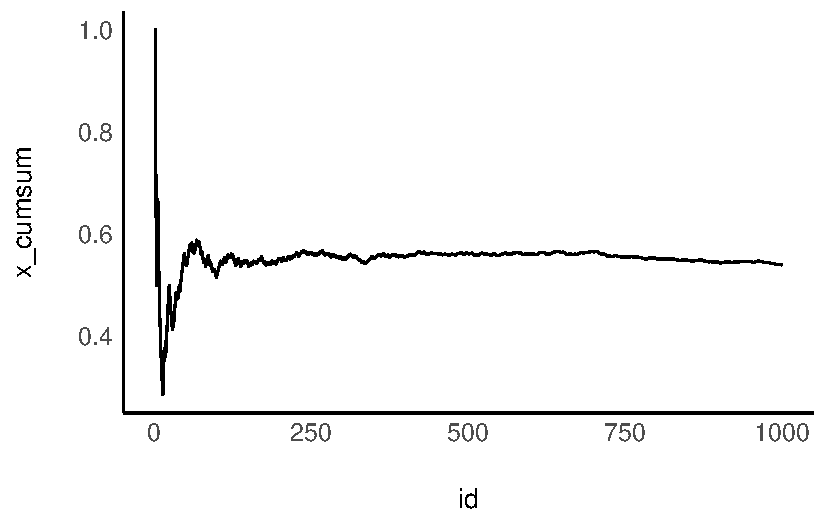
\includegraphics{./Verteilungen_files/figure-pdf/fig-lln-1.pdf}

}

\caption{\label{fig-lln}Das Gesetz der großen Zahl am Beispiel der
Stabilisierung des Trefferanteils beim wiederholten Münzwurf}

\end{figure}

Grob gesagt scheint sich ein Münzwurf nach, naja, vielleicht 500 Würfen
``einigermaßen'' zu stabilisieren.\footnote{Was ``einigermaßen''
  bedeuten soll, ist kein statistischer Begriff, sondern einer, der im
  echten Leben von den Menschen beantwortet werden muss, die eine
  Entscheidung zu treffen haben.}

\begin{tcolorbox}[enhanced jigsaw, colframe=quarto-callout-important-color-frame, breakable, titlerule=0mm, left=2mm, colbacktitle=quarto-callout-important-color!10!white, opacityback=0, colback=white, opacitybacktitle=0.6, toptitle=1mm, rightrule=.15mm, toprule=.15mm, bottomrule=.15mm, bottomtitle=1mm, title=\textcolor{quarto-callout-important-color}{\faExclamation}\hspace{0.5em}{Wichtig}, leftrule=.75mm, arc=.35mm, coltitle=black]

Das Gesetz der großen Zahl

Zieht man (zufällig) immer mehr Werte aus einer Verteilung (mit
endlichem Mittelwert), nähert sich der Mittelwert der Stichprobe immer
mehr mit dem Mittelwert (oft als Erwartungswert bezeichnet) der
Verteilung an

\end{tcolorbox}

\hypertarget{normalverteilung}{%
\section{Normalverteilung}\label{normalverteilung}}

Normalverteilungen haben eine charakteristische Glockenform.
Normalverteilungen können sich unterscheiden in ihrem Mittelwert \(\mu\)
und ihrer Streuung, \(\sigma\). Diese beiden Größen (``Parameter'')
determinieren den Graphen einer bestimmten Normalverteilungsfunktion, s.
Abbildung~\ref{fig-norms}. Sind diese beiden Parameter bekannt, so ist
die Dichte jedes beliebigen Datenpunkts (aus dieser Normalverteilung)
bestimmt.

\begin{figure}

{\centering 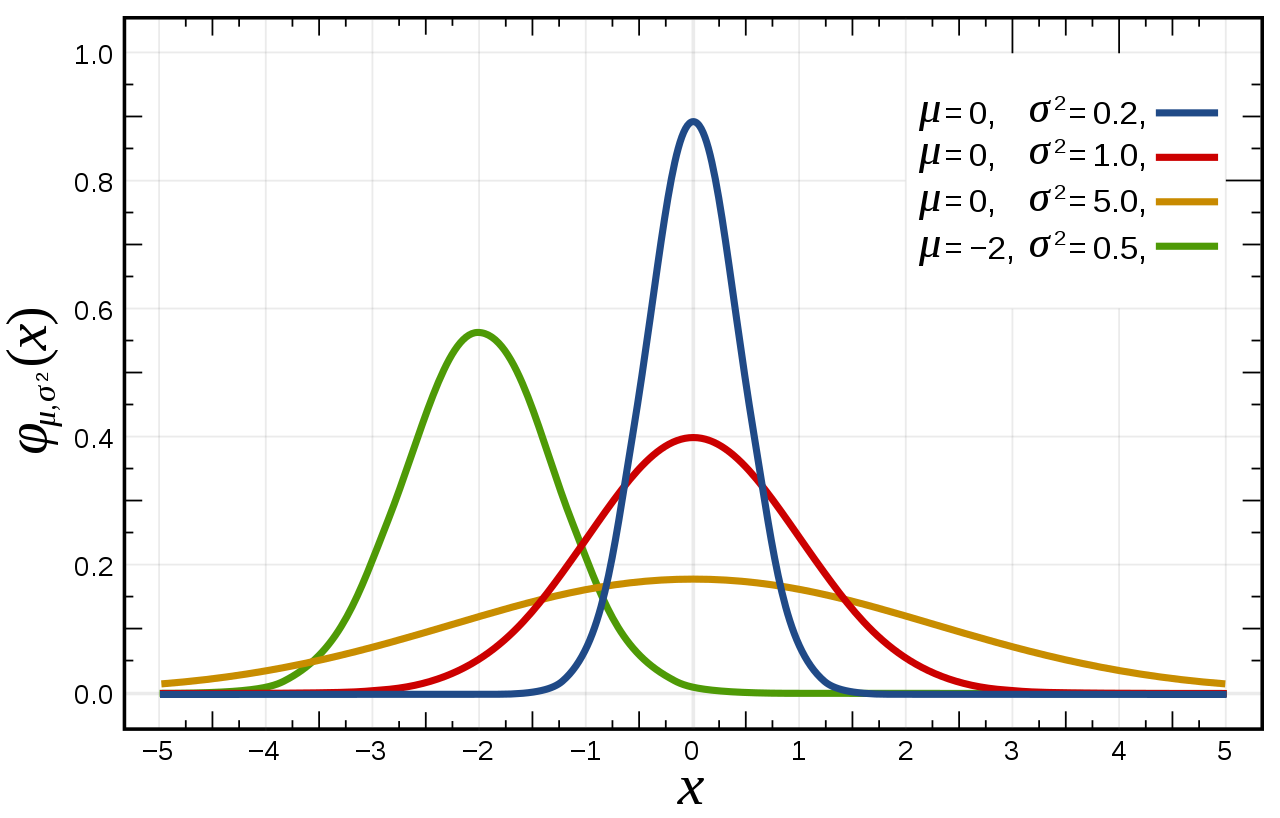
\includegraphics[width=0.5\textwidth,height=\textheight]{./img/normals.png}

}

\caption{\label{fig-norms}Beispiele von Normalverteilungen mit
verschiedenen Mittelwerten und Streuungen, Quelle: Wikipedia}

\end{figure}

Beispiel: Wie groß sind Studentis
(\href{https://rdrr.io/cran/openintro/man/speed_gender_height.html}{Quelle
des Datensatzes})?

Das Quantil von z.B. 25\% zeigt die Körpergröße der 25\% kleinsten
Studentis an, analog für 50\%, 75\%:

\begin{longtable}{rrr}
\toprule
q25 & q50 & q75 \\ 
\midrule
160.02 & 167.64 & 175.26 \\ 
\bottomrule
\end{longtable}

Abbildung~\ref{fig-quantiles} zeigt eine Visualisierung der Quantile.

\begin{figure}

{\centering 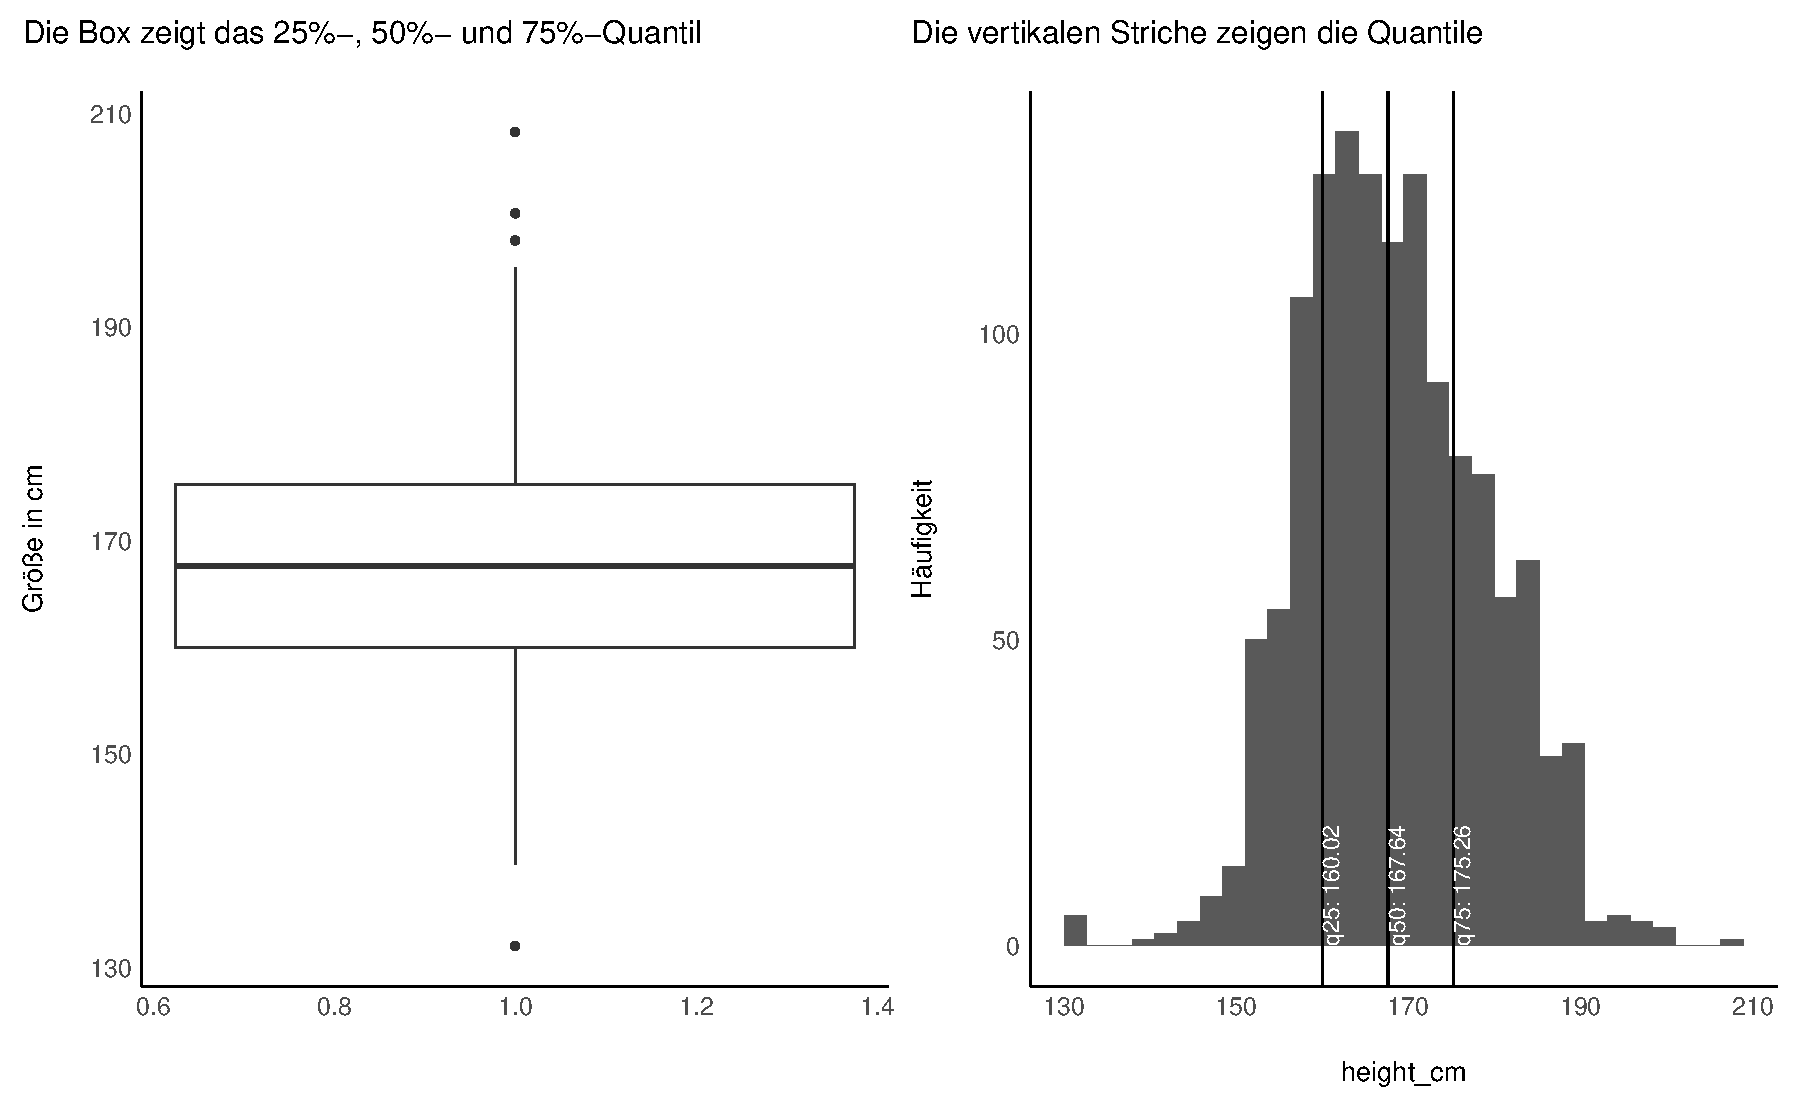
\includegraphics{./Verteilungen_files/figure-pdf/fig-quantiles-1.pdf}

}

\caption{\label{fig-quantiles}Quantile verschieden visualisiert}

\end{figure}

\begin{tcolorbox}[enhanced jigsaw, colframe=quarto-callout-note-color-frame, breakable, titlerule=0mm, left=2mm, colbacktitle=quarto-callout-note-color!10!white, opacityback=0, colback=white, opacitybacktitle=0.6, toptitle=1mm, rightrule=.15mm, toprule=.15mm, bottomrule=.15mm, bottomtitle=1mm, title=\textcolor{quarto-callout-note-color}{\faInfo}\hspace{0.5em}{Hinweis}, leftrule=.75mm, arc=.35mm, coltitle=black]

Das 25\%-Quantil nennt man \emph{1. Quartil}, das 50\%-Quantil auch
\emph{2. Quartil}, das 75\%-Quantil das \emph{3. Quartil}, und das
100\%-Quantil (Maximalwert) das \emph{4. Quartil}.

\end{tcolorbox}

\hypertarget{normal-auf-dem-fuuxdfballfeld}{%
\subsection{Normal auf dem
Fußballfeld}\label{normal-auf-dem-fuuxdfballfeld}}

Sie und 100 Ihrer besten Freunde stehen auf der Mittellinie eines
Fußballfelds. Auf Kommando werfen alle jeweils eine Münze; bei Kopf geht
man einen Schritt nach links, bei Zahl nach rechts. Das wird 16 Mal
wiederholt. Wie wird die Verteilung der Positionen wohl aussehen?

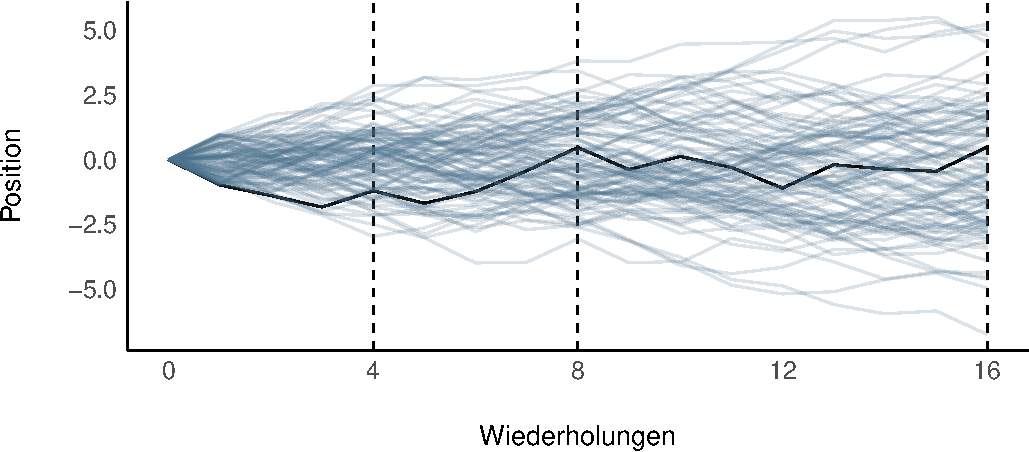
\includegraphics{./Verteilungen_files/figure-pdf/Normalverteilung-6-1.pdf}

(McElreath 2020)

\hypertarget{normal-durch-addieren}{%
\subsection{Normal durch Addieren}\label{normal-durch-addieren}}

Die Summe vieler (gleich starker) Zufallswerte (aus der gleichen
Verteilung) erzeugt eine Normalverteilung; egal aus welcher Verteilung
die Zufallswerte kommen (Zentraler Grenzwertsatz), vgl.
Abbildung~\ref{fig-fussball}.

\begin{figure}

{\centering 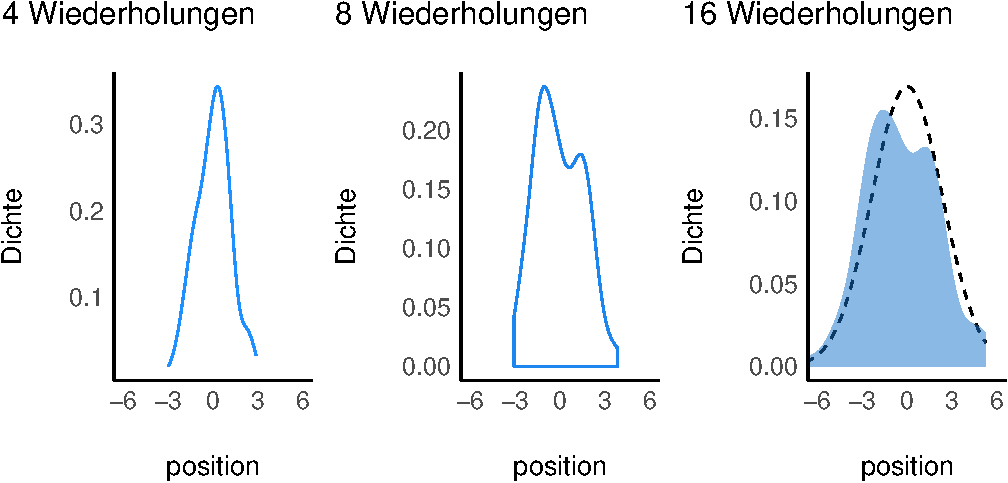
\includegraphics[width=1\textwidth,height=\textheight]{./Verteilungen_files/figure-pdf/fig-fussball-1.pdf}

}

\caption{\label{fig-fussball}Entstehen einer Normalverteilung durch
Addition vieler unabhgängiger Ereignisse}

\end{figure}

Nicht verwechseln:

\begin{figure}

{\centering 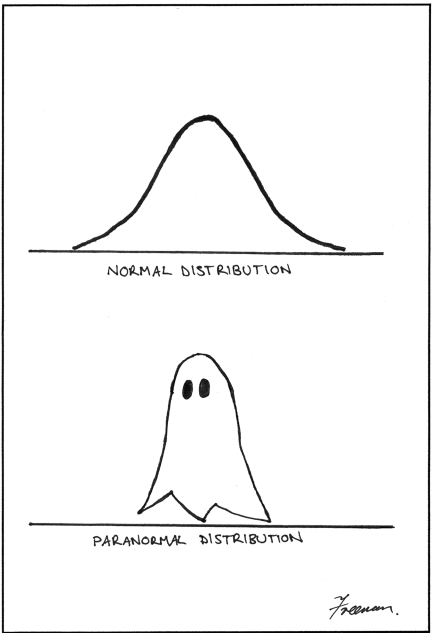
\includegraphics[width=0.3\textwidth,height=\textheight]{./img/ch33910f1.jpg}

}

\end{figure}

\hypertarget{normalverteilung-vs.-randlastige-verteilungen}{%
\subsection{Normalverteilung vs.~randlastige
Verteilungen}\label{normalverteilung-vs.-randlastige-verteilungen}}

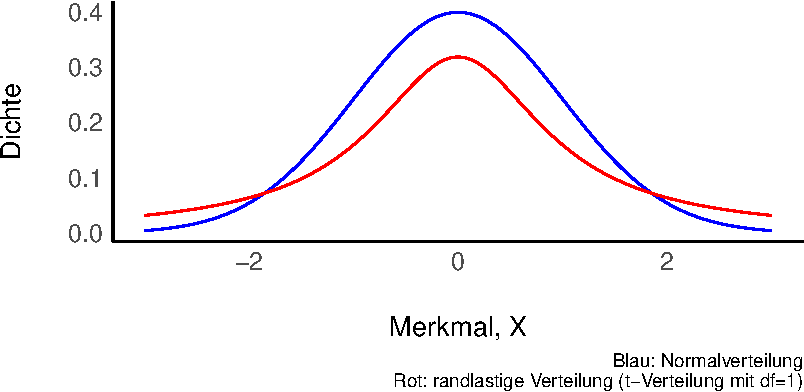
\includegraphics{./Verteilungen_files/figure-pdf/Normalverteilung-9-1.pdf}

Bei randlastigen Verteilungen (``fat tails'') kommen Extremereignisse
viel häufiger vor als bei Normalverteilungen. Deshalb ist es wichtig
sein, zu wissen, ob eine Normalverteilung oder eine randlastige
Verteilung vorliegt. Viele statistische Methoden sind nicht zuverlässig
bei (stark) randlastigen Methoden.

\hypertarget{beispiele-fuxfcr-normal--und-randlastige-verteilungen}{%
\subsection{Beispiele für Normal- und randlastige
Verteilungen}\label{beispiele-fuxfcr-normal--und-randlastige-verteilungen}}

Normal verteilt:

\begin{itemize}
\tightlist
\item
  Größe
\item
  Münzwürfe
\item
  Gewicht
\item
  IQ
\item
  Blutdruck
\item
  Ausschuss einer Maschine
\end{itemize}

Randlastig verteilt:

\begin{itemize}
\tightlist
\item
  Vermögen
\item
  Verkaufte Bücher
\item
  Ruhm
\item
  Aktienkurse
\item
  Erdbeben
\item
  Pandemien
\item
  Kriege
\item
  Erfolg auf Tinder
\item
  Meteroritengröße
\item
  Stadtgrößen
\end{itemize}

\hypertarget{formel-der-normalverteilung}{%
\subsection{Formel der
Normalverteilung}\label{formel-der-normalverteilung}}

Vereinfacht ausgedrückt lässt die Normalverteilung \(\mathcal{N}\) durch
Exponenzieren einer Quadratfunktion beschreiben:

\[\mathcal{N} \propto e^{-x^2}\]

mit \(e=2.71...\), der Eulerschen Zahl.\footnote{Das Zeichen
  \(y \propto x\) bedeutet ``x ist proportional zu y'', also \(y = mx\).}

\begin{Shaded}
\begin{Highlighting}[]
\NormalTok{d }\OtherTok{\textless{}{-}}
  \FunctionTok{tibble}\NormalTok{(}
    \AttributeTok{x =} \FunctionTok{seq}\NormalTok{(}\SpecialCharTok{{-}}\DecValTok{3}\NormalTok{, }\DecValTok{3}\NormalTok{, }
            \AttributeTok{length.out =} \DecValTok{100}\NormalTok{),}
    \AttributeTok{y =} \FunctionTok{exp}\NormalTok{(}\SpecialCharTok{{-}}\NormalTok{x}\SpecialCharTok{\^{}}\DecValTok{2}\NormalTok{)}
\NormalTok{  )}

\NormalTok{d }\SpecialCharTok{\%\textgreater{}\%} 
  \FunctionTok{ggplot}\NormalTok{() }\SpecialCharTok{+}
  \FunctionTok{aes}\NormalTok{(}\AttributeTok{x =}\NormalTok{ x, }\AttributeTok{y =}\NormalTok{ y) }\SpecialCharTok{+}
  \FunctionTok{geom\_line}\NormalTok{()}
\end{Highlighting}
\end{Shaded}

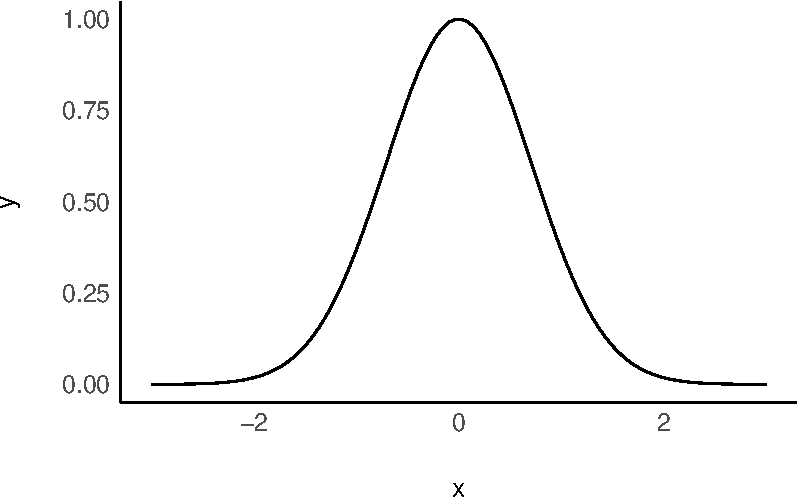
\includegraphics{./Verteilungen_files/figure-pdf/Normalverteilung-10-1.pdf}

Eine Normalverteilung mit \(\mu=0\) und \(\sigma=1\) nennt man auch
\emph{Standardnormalverteilung} und man schreibt:

\[IQ \sim \mathcal{N}(0,1)\]

Die Normalverteilung wird auch
\emph{\href{https://de.wikipedia.org/wiki/Carl_Friedrich_Gau\%C3\%9F}{Gauss}-Verteilung}
oder \emph{Glockenkurve} genannt.

\hypertarget{simulation-einer-normalverteilung}{%
\subsection{Simulation einer
Normalverteilung}\label{simulation-einer-normalverteilung}}

R hat eine Funktion eingebaut zur Erzeugung von Zufallszahlen
(Zufallszahlengenerator), z.B. normalverteilte. Man übergibt dieser
Funktion den gewünschten Mittelwert und die gewünschte Streuung und die
Funktion zieht dann zufällig Werte aus dieser Verteilung.

Diesen Zufallszahlengenerator kann man mit einem Duschkopf vergleichen,
s. Abbildung~\ref{fig-shower}. An diesem Duschkopf kann man einen
Schwenker einstellen, der den Duschkopf ausrichtet, also steuert, ob die
Wassertropfen weit in die eine oder die andere Richtugn fallen. Zweitens
hat unser Duschkopf noch einen Streuregler, der den Wasserstrahl
entweder eng bündelt\footnote{Massagedusche, behauptet der Hersteller}
oder weit auseinanderfächert. Im ersten Fall fällt der Wasserstrahl eng
und schmal aus. Im zweiten Fall fällt der Wasserstrahl breit aus.

\begin{figure}

{\centering 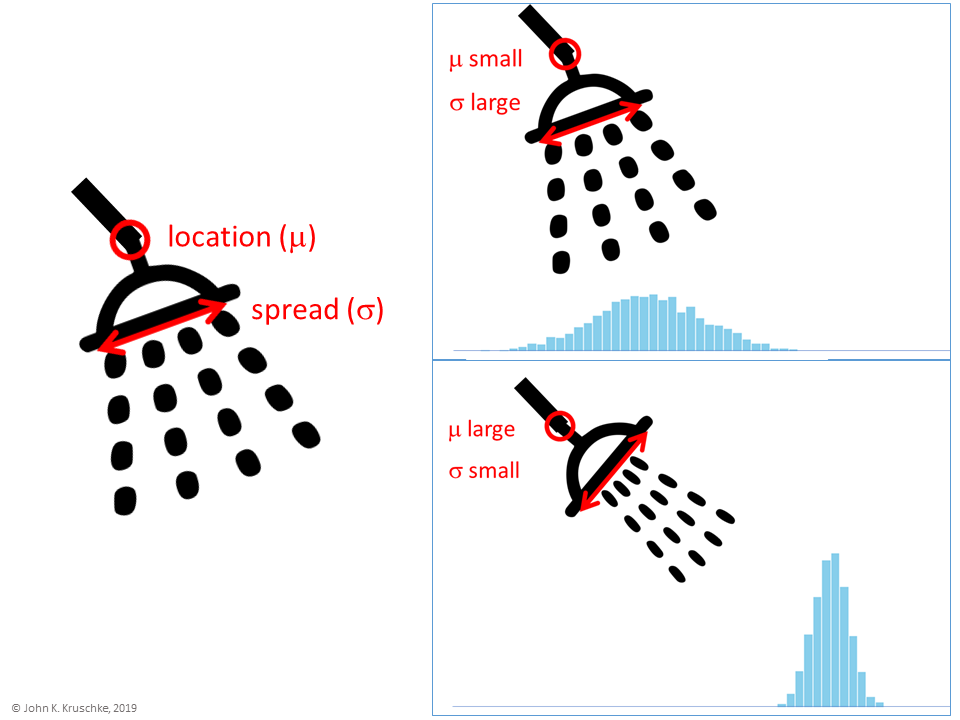
\includegraphics[width=0.5\textwidth,height=\textheight]{./img/shower-data.png}

}

\caption{\label{fig-shower}Zufallszahlengenerator als Duschkopf}

\end{figure}

\href{https://jkkweb.sitehost.iu.edu/KruschkeFreqAndBayesAppTutorial.html\#data_are_described_by_mathematical_models}{Quelle}:
John Kruschke.

Eine Zufallszahl (\emph{r}andom number), die \emph{norm}alverteilt ist,
mit \(\mu=0\) und \(\sigma=1\) kann man in R so erzeugen:

\begin{Shaded}
\begin{Highlighting}[]
\FunctionTok{rnorm}\NormalTok{(}\AttributeTok{n =} \DecValTok{1}\NormalTok{, }\AttributeTok{mean =} \DecValTok{0}\NormalTok{, }\AttributeTok{sd =} \DecValTok{1}\NormalTok{)}
\DocumentationTok{\#\# [1] 0.2664096}
\end{Highlighting}
\end{Shaded}

Ein Fallbeispiel: Der Inhalt einer Tüte mit Zucker, \(X\), sei
normalverteilt mit \(\mu = 10002\) g und \(\sigma=1.5\) g. Aus
vertragsrechtlichen Gründen darf das Füllgewicht von 1000g nicht
unterschritten werden, sonst drohen Konventionalstrafen.

Wie groß ist die Wahrscheinlichkeit, dass 1000g unterschritten werden?

Simulieren wir uns 1e4 Zuckertüten!

\begin{Shaded}
\begin{Highlighting}[]
\NormalTok{n }\OtherTok{\textless{}{-}} \FloatTok{1e4}
\NormalTok{d }\OtherTok{\textless{}{-}} 
  \FunctionTok{tibble}\NormalTok{(}
    \AttributeTok{id =} \DecValTok{1}\SpecialCharTok{:}\NormalTok{n,}
    \AttributeTok{x =} \FunctionTok{rnorm}\NormalTok{(}\AttributeTok{n =}\NormalTok{ n, }\AttributeTok{mean =} \DecValTok{1002}\NormalTok{, }\AttributeTok{sd =} \FloatTok{1.5}\NormalTok{)}
\NormalTok{  )}

\FunctionTok{head}\NormalTok{(d)}
\end{Highlighting}
\end{Shaded}

\begin{longtable}[]{@{}rr@{}}
\toprule()
id & x \\
\midrule()
\endhead
1 & 1002.479 \\
2 & 1001.216 \\
3 & 1003.320 \\
4 & 1001.173 \\
5 & 1001.465 \\
6 & 1003.843 \\
\bottomrule()
\end{longtable}

Zählen wir, viele der Zuckertüten ein Gewicht von weniger als 1000g
aufweisen:

\begin{Shaded}
\begin{Highlighting}[]
\NormalTok{d }\SpecialCharTok{\%\textgreater{}\%} 
  \FunctionTok{count}\NormalTok{(x }\SpecialCharTok{\textless{}} \DecValTok{1000}\NormalTok{)}
\end{Highlighting}
\end{Shaded}

\begin{longtable}[]{@{}lr@{}}
\toprule()
x \textless{} 1000 & n \\
\midrule()
\endhead
FALSE & 9013 \\
TRUE & 987 \\
\bottomrule()
\end{longtable}

Ein ziemlich\footnote{``Ziemlich'' ist natürlich subjektiv; je nach
  Situation kann es zu viel oder nicht zu viel sein.} kleiner Anteil.
Rechnen wir uns noch die Anteile (\emph{prop}ortion) aus:

\begin{Shaded}
\begin{Highlighting}[]
\NormalTok{d }\SpecialCharTok{\%\textgreater{}\%} 
  \FunctionTok{count}\NormalTok{(x }\SpecialCharTok{\textless{}} \DecValTok{1000}\NormalTok{) }\SpecialCharTok{\%\textgreater{}\%} 
  \FunctionTok{mutate}\NormalTok{(}\AttributeTok{prop =}\NormalTok{ n}\SpecialCharTok{/}\FloatTok{1e4}\NormalTok{)}
\end{Highlighting}
\end{Shaded}

\begin{longtable}[]{@{}lrr@{}}
\toprule()
x \textless{} 1000 & n & prop \\
\midrule()
\endhead
FALSE & 9013 & 0.9013 \\
TRUE & 987 & 0.0987 \\
\bottomrule()
\end{longtable}

\hypertarget{iq-verteilung}{%
\subsection{IQ-Verteilung}\label{iq-verteilung}}

Die Verteilung der Zufallsvariablen IQ ist normalverteilt mit einem
Mittelwert von 100 und einer Streuung von 15, s.
Abbildung~\ref{fig-norm-100-15}:

\(IQ \sim \mathcal{N}(100,15)\)

\begin{itemize}
\tightlist
\item
  Wie schlau muss man sein, um zu den unteren 75\%, 50\%, 25\%, 5\%, 1\%
  zu gehören?
\item
  Anders gesagt: Welcher IQ-Wert wird von 75\%, 50\%, \ldots{} der Leute
  nicht überschritten?
\end{itemize}

\begin{figure}

{\centering 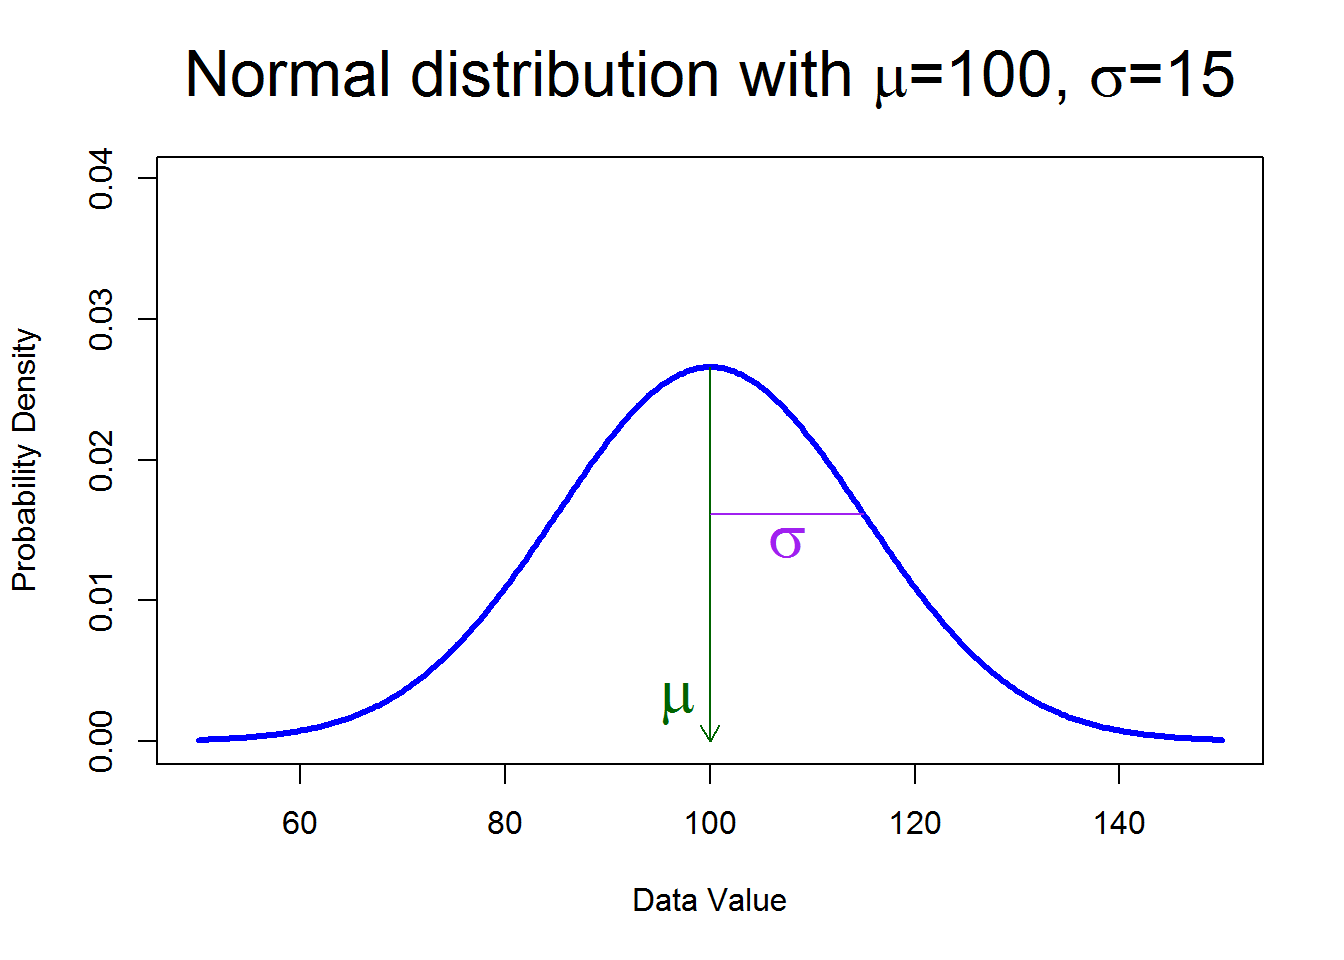
\includegraphics[width=0.5\textwidth,height=\textheight]{./img/norm-100-15.png}

}

\caption{\label{fig-norm-100-15}Visualisierung der theoretischen
IQ-Verteilung}

\end{figure}

\href{https://jkkweb.sitehost.iu.edu/KruschkeFreqAndBayesAppTutorial.html\#data_are_described_by_mathematical_models}{Quelle:}:
John Kruschke.

Ziehen wir zufällig \(1e4\) Stichproben aus \(\mathcal{N}(100,15)\) und
berechnen die Quantile:

\begin{Shaded}
\begin{Highlighting}[]
\NormalTok{d }\OtherTok{\textless{}{-}}
  \FunctionTok{tibble}\NormalTok{(}
  \AttributeTok{iq =} \FunctionTok{rnorm}\NormalTok{(}\AttributeTok{n =} \FloatTok{1e4}\NormalTok{, }
             \AttributeTok{mean =} \DecValTok{100}\NormalTok{, }
             \AttributeTok{sd =} \DecValTok{15}\NormalTok{))}

\NormalTok{probs }\OtherTok{\textless{}{-}} \FunctionTok{c}\NormalTok{(}\FloatTok{0.75}\NormalTok{,.}\DecValTok{5}\NormalTok{,.}\DecValTok{25}\NormalTok{,.}\DecValTok{05}\NormalTok{,.}\DecValTok{01}\NormalTok{)}

\NormalTok{d\_summary }\OtherTok{\textless{}{-}}\NormalTok{ d }\SpecialCharTok{\%\textgreater{}\%} 
  \FunctionTok{summarise}\NormalTok{(}\AttributeTok{p =}\NormalTok{ probs,}
            \AttributeTok{q =} \FunctionTok{quantile}\NormalTok{(iq, probs))}
\end{Highlighting}
\end{Shaded}

\begin{longtable}{rr}
\toprule
p & q \\ 
\midrule
$0.75$ & $110$ \\ 
$0.50$ & $100$ \\ 
$0.25$ & $90$ \\ 
$0.05$ & $75$ \\ 
$0.01$ & $65$ \\ 
\bottomrule
\end{longtable}

Das \emph{Quantil} \(q\) zur kumulierten Wahrscheinlichkeit \(p=75\) ist
110, etc.

Umgekehrt können wir uns auch fragen: Gegeben einer Realisation der
Zufallsvariablen (z.B. IQ), was ist die zugehörige Wahrscheinlichkeit
(Wert der Verteilungsfunktion?)

\begin{itemize}
\tightlist
\item
  Welcher Anteil der Fläche unter der Kurve \(p\) gehört zu den
  IQ-Werten 75, 100, 115, 130?
\item
  Anders gesagt: Welcher Anteil der Wahrscheinlichkeitsmasse der
  Verteilung liegt unter IQ=75, IQ=100, etc.?
\end{itemize}

Ziehen wir Stichproben aus \(\mathcal{N}(100,15)\):

\begin{Shaded}
\begin{Highlighting}[]
\NormalTok{d }\OtherTok{\textless{}{-}}
  \FunctionTok{tibble}\NormalTok{(}
    \AttributeTok{iq =} \FunctionTok{rnorm}\NormalTok{(}\FloatTok{1e4}\NormalTok{, }
               \AttributeTok{mean =} \DecValTok{100}\NormalTok{, }
               \AttributeTok{sd =} \DecValTok{15}\NormalTok{)) }\SpecialCharTok{\%\textgreater{}\%} 
  \FunctionTok{mutate}\NormalTok{(}\AttributeTok{iq =} \FunctionTok{round}\NormalTok{(iq))}

\NormalTok{qs }\OtherTok{\textless{}{-}} \FunctionTok{c}\NormalTok{(}\DecValTok{75}\NormalTok{,}\DecValTok{100}\NormalTok{,}\DecValTok{115}\NormalTok{,}\DecValTok{130}\NormalTok{)}

\NormalTok{d }\SpecialCharTok{\%\textgreater{}\%} 
  \FunctionTok{count}\NormalTok{(}\AttributeTok{p\_100 =}\NormalTok{ iq }\SpecialCharTok{\textless{}} \DecValTok{100}\NormalTok{) }\SpecialCharTok{\%\textgreater{}\%} 
  \FunctionTok{mutate}\NormalTok{(}\AttributeTok{prop =}\NormalTok{ n }\SpecialCharTok{/} \FunctionTok{sum}\NormalTok{(n)) }
\end{Highlighting}
\end{Shaded}

\begin{longtable}{crr}
\toprule
p\_100 & n & prop \\ 
\midrule
FALSE & 5143 & $0.51$ \\ 
TRUE & 4857 & $0.49$ \\ 
\bottomrule
\end{longtable}

Anstelle von \texttt{iq\ \textless{}\ 100} kann man
\texttt{iq\ \textless{}\ 115} einsetzen, etc.

Die \emph{Verteilungsfunktion} (der Anteil der
Wahrscheinlichkeitsmasse), \texttt{p}, für IQ-Werte nicht größer als
100, \(IQ\le100\), ist 50\%, etc.

\hypertarget{quantile-der-normalverteilung}{%
\subsection{Quantile der
Normalverteilung}\label{quantile-der-normalverteilung}}

\begin{itemize}
\tightlist
\item
  \emph{Quantile} teilen eine Verteilung so ein, dass ein Anteil \(p\)
  kleiner oder gleich und der andere Teil \(1-p\) größer dem Quantil
  \(q\) ist.

  \begin{itemize}
  \tightlist
  \item
    \emph{Beispiel}: ``50\%-Quantil = 100'' meint, dass 50\% der
    Elemente der Verteilung einen Wert kleiner oder gleich als 100
    haben.
  \end{itemize}
\item
  Die \emph{Verteilungsfunktion F} (für einen Wert \(x\)) gibt die
  Wahrscheinlichkeit an, dass die zugehörige Zufallsvariable \(X\) einen
  Wert höchstens so groß wie \(x\) annimmt. Sie zeigt also die
  kumulierte Wahrscheinlichkeit \([-\infty, q)\).

  \begin{itemize}
  \tightlist
  \item
    \emph{Beispiel}: ``F(100) = 50\%'' meint: Die Wahrscheinlichkeit für
    eine Ausprägung von höchstens als 100 beträgt 50\%.
  \end{itemize}
\end{itemize}

Schauen wir uns die Quartile der Normalverteilung einmal näher an. Wir
gehen von einer Normalverteilung aus, wie sie zur Beschreibung von
Intelligenz (IQ) verwendet wird, s. Abbildung~\ref{fig-nv-quants}.

\begin{figure}

{\centering \includegraphics{./Verteilungen_files/figure-pdf/fig-nv-quants-1.pdf}

}

\caption{\label{fig-nv-quants}Quantile der Normalverteiltung}

\end{figure}

\[IQ \sim \mathcal{N}(100, 15)\] Mit R kann man sich die beiden Größen
komfortabel berechnen lassen:

\begin{Shaded}
\begin{Highlighting}[]
\FunctionTok{qnorm}\NormalTok{(.}\DecValTok{50}\NormalTok{, }\AttributeTok{mean =} \DecValTok{100}\NormalTok{, }\AttributeTok{sd =} \DecValTok{15}\NormalTok{)  }\CommentTok{\# 50\%{-}Quantil}
\FunctionTok{pnorm}\NormalTok{(}\DecValTok{100}\NormalTok{, }\AttributeTok{mean =} \DecValTok{100}\NormalTok{, }\AttributeTok{sd =} \DecValTok{15}\NormalTok{)  }\CommentTok{\# Verteilungsfunktion für IQ=100}
\end{Highlighting}
\end{Shaded}

Betrachten wir einige wichtigen Quantile, s.
Abbildung~\ref{fig-nv-quants2}.

\begin{figure}

{\centering \includegraphics{./Verteilungen_files/figure-pdf/fig-nv-quants2-1.pdf}

}

\caption{\label{fig-nv-quants2}Verschiedene Quantil der
Normalverteilung}

\end{figure}

\hypertarget{standardnormalverteilung}{%
\subsection{Standardnormalverteilung}\label{standardnormalverteilung}}

\includegraphics{./Verteilungen_files/figure-pdf/Normalverteilung-3-1.pdf}

Bei \(X=0\):

\begin{itemize}
\tightlist
\item
  hat eine Einheit von \(X\) die Wahrscheinlichkeitsmasse von 40\%
  (Wahrscheinlichkeitsdichte)
\item
  sind 50\% der Wahrscheinlichkeitsmasse (Fläche unter der Kurve)
  kleiner als dieser Wert (Verteilungsfunktion).
\end{itemize}

In Summe liegen 100\% der Wahrscheinlichkeitsmasse unter der Kurve.

\hypertarget{normalverteilung-als-konservative-wahl}{%
\subsection{Normalverteilung als konservative
Wahl}\label{normalverteilung-als-konservative-wahl}}

Dem Mathematiker
\href{https://de.wikipedia.org/wiki/Carl_Friedrich_Gau\%C3\%9F}{Carl
Friedrich Gauss} (s. Abbildung~\ref{fig-gauss}) wird die Ehre zuerkannt,
die Normalverteilung eingeführt zu haben.

\begin{figure}

{\centering \includegraphics[width=2.27in,height=\textheight]{./img/10_Deutsche_Mark_-_detail.png}

}

\caption{\label{fig-gauss}Zehn-Mark-Geldschein mit Gauss und
Normalverteilung}

\end{figure}

Quelle: Uni Greifswald, Public domain, via Wikimedia Commons

\begin{tcolorbox}[enhanced jigsaw, colframe=quarto-callout-note-color-frame, breakable, titlerule=0mm, left=2mm, colbacktitle=quarto-callout-note-color!10!white, opacityback=0, colback=white, opacitybacktitle=0.6, toptitle=1mm, rightrule=.15mm, toprule=.15mm, bottomrule=.15mm, bottomtitle=1mm, title=\textcolor{quarto-callout-note-color}{\faInfo}\hspace{0.5em}{Hinweis}, leftrule=.75mm, arc=.35mm, coltitle=black]

\emph{Ontologische Begründung}

\begin{itemize}
\tightlist
\item
  Wirken viele, gleichstarke Einflüsse additiv zusammen, entsteht eine
  Normalverteilung (McElreath 2020), Kap. 4.1.4.
\end{itemize}

\emph{Epistemologische Begründung}

\begin{itemize}
\tightlist
\item
  Wenn wir nur wissen, dass eine Variable über einen endlichen
  Mittelwert und eine endliche Varianz verfügt und wir keine weiteren
  Annahmen treffen bzw. über kein weiteres Vorwissen verfügen, dann ist
  die Normalverteilung die plausibelste Verteilung (maximale Entropie)
  (McElreath 2020), Kap. 7 und 10.
\end{itemize}

\end{tcolorbox}

\hypertarget{aufgaben-2}{%
\section{Aufgaben}\label{aufgaben-2}}

Zusätzlich zu den Aufgaben im Buch:

\begin{itemize}
\tightlist
\item
  \href{https://datenwerk.netlify.app/posts/lose-nieten-binomial-grid/lose-nieten-binomial-grid}{Lose-Nieten-Binomial-Grid}
\item
  \href{https://datenwerk.netlify.app/posts/bsp-binomial/bsp-binomial}{Bsp-Binomial}
\end{itemize}

\hypertarget{section-3}{%
\section{---}\label{section-3}}

\includegraphics[width=1\textwidth,height=\textheight]{./img/outro-04.jpg}

\bookmarksetup{startatroot}

\hypertarget{globusversuch}{%
\chapter{Globusversuch}\label{globusversuch}}

\begin{figure}

{\centering \includegraphics[width=0.05\textwidth,height=\textheight]{./img/Golem_hex.png}

}

\caption{Bayes:Start}

\end{figure}

\hypertarget{lernsteuerung-3}{%
\section{Lernsteuerung}\label{lernsteuerung-3}}

\hypertarget{lernziele-4}{%
\subsection{Lernziele}\label{lernziele-4}}

Nach Absolvieren des jeweiligen Kapitels sollen folgende Lernziele
erreicht sein.

Sie können \ldots{}

\begin{itemize}
\tightlist
\item
  Unterschiede zwischen Modellen und der Realität erläutern
\item
  die Binomialverteilung heranziehen, um geeignete (einfache) Modelle zu
  erstellen
\item
  die weite Einsetzbarkeit anhand mehrerer Beispiele exemplifizieren
\item
  Post-Wahrscheinlichkeiten anhand der Gittermethode berechnen
\end{itemize}

\hypertarget{benuxf6tigte-r-pakete-1}{%
\subsection{Benötigte R-Pakete}\label{benuxf6tigte-r-pakete-1}}

\begin{Shaded}
\begin{Highlighting}[]
\FunctionTok{library}\NormalTok{(tidyverse)}
\end{Highlighting}
\end{Shaded}

\hypertarget{begleitvideos-3}{%
\subsection{Begleitvideos}\label{begleitvideos-3}}

\begin{itemize}
\tightlist
\item
  \href{https://youtu.be/fGlt9Ld4xzk}{Video zum Thema Globusversuch}
\item
  \href{https://youtu.be/YJEZiQvCBgs}{Video zum Thema Übungen zum
  Globusversuch}
\end{itemize}

\hypertarget{von-welten-und-golems}{%
\section{Von Welten und Golems}\label{von-welten-und-golems}}

\hypertarget{kleine-welt-grouxdfe-welt}{%
\subsection{Kleine Welt, große Welt}\label{kleine-welt-grouxdfe-welt}}

Bekanntlich segelte Kolumbus 1492 los, und entdeckte Amerika\footnote{wenn
  auch nicht als Erster}. Das war aber ein glücklicher Zufall, denn auf
seinem Globus existierte Amerika gar nicht. Vielleicht sah sein Globus
so aus wie der von Behaim, s. Abb Abbildung~\ref{fig-behaim}.

\begin{figure}

{\centering \includegraphics{./img/Behaim.jpg}

}

\caption{\label{fig-behaim}Behaims Globus: Kein Amerika}

\end{figure}

\href{https://commons.wikimedia.org/wiki/File:RavensteinBehaim.jpg}{Quelle:
Ernst Ravenstein, Wikimedia, Public Domain}

Die \emph{kleine Welt des Modells} entsprach hier nicht \emph{der großen
Welt, der echten Erdkugel}.

Das ist ein Beispiel, das zeigt, wie Modellieren schiefgehen kann. Es
ist aber auch ein Beispiel für, sagen wir, die Komplexität
wissenschaftlicher (und sonstiger) Erkenntnis. Einfach gesagt: Glück
gehört halt auch dazu.

\begin{tcolorbox}[enhanced jigsaw, colframe=quarto-callout-note-color-frame, breakable, titlerule=0mm, left=2mm, colbacktitle=quarto-callout-note-color!10!white, opacityback=0, colback=white, opacitybacktitle=0.6, toptitle=1mm, rightrule=.15mm, toprule=.15mm, bottomrule=.15mm, bottomtitle=1mm, title=\textcolor{quarto-callout-note-color}{\faInfo}\hspace{0.5em}{Hinweis}, leftrule=.75mm, arc=.35mm, coltitle=black]

Behaims Globus ist nicht gleich der Erde. Die kleine Welt von Behaims
Globus ist nicht die große Welt, ist nicht die Erde.

\end{tcolorbox}

Was in der kleinen Welt funktioniert, muss nicht in der großen Welt
funktionieren. Modelle zeigen immer nur die kleine Welt: Vorsicht vor
schnellen Schlüssen und vermeintlicher Gewissheit.

🏋 Nennen Sie ein Beispiel, in dem ein Modell nicht (exakt) der
Wirklichkeit entspricht!

\hypertarget{der-golem-von-prag}{%
\subsection{Der Golem von Prag}\label{der-golem-von-prag}}

\begin{figure}

{\centering \includegraphics[width=0.33\textwidth,height=\textheight]{./img/170px-Golem_and_Loew.jpg}

}

\caption{\label{fig-golem-prag}Der Golem von Prag}

\end{figure}

\href{https://de.wikipedia.org/wiki/Golem}{Quelle}

\href{http://www.prague.net/golem}{Der Golem von Prag}, die Legende
einer vom Menschen geschaffene Kreatur mit gewaltiger Kraft, die Befehle
wörtlich ausführt, s. Abbildung~\ref{fig-golem-prag}. Die Geschichte
besagt, dass ein Rabbi mit Zauberkräften den Golem aus Lehm erschuf, um
die jüdische Bevölkerung der Stadt zu schätzen. Bei kluger Führung kann
ein Golem Nützliches vollbringen. Bei unüberlegter Verwendung wird er
jedoch großen Schaden anrichten.

\hypertarget{wissenschaftliche-modelle-sind-wie-golems}{%
\subsection{Wissenschaftliche Modelle sind wie
Golems}\label{wissenschaftliche-modelle-sind-wie-golems}}

\textbf{Golem}

\begin{figure}

{\centering \includegraphics[width=0.25\textwidth,height=\textheight]{./img/Golem_hex.png}

}

\caption{``Yeah, ich bin ein Golem!'' - Bildquelle: Klara Schaumann}

\end{figure}

Eigenschaften des \emph{Golems}:

\begin{itemize}
\tightlist
\item
  Besteht aus Lehm
\item
  Belebt durch ``Wahrheit''
\item
  Mächtig
\item
  dumm
\item
  Führt Befehle wörtlich aus
\item
  Missbrauch leicht möglich
\item
  Märchen
\end{itemize}

\textbf{Modell}

Eigenschaften eines \emph{Modells}:

\begin{itemize}
\tightlist
\item
  Besteht aus \sout{Lehm}Silikon
\item
  Belebt durch Wahrheit (?)
\item
  Manchmal mächtig
\item
  simpler als die Realität
\item
  Führt Befehle wörtlich aus
\item
  Missbrauch leicht möglich
\item
  Nicht einmal falsch
\end{itemize}

\begin{tcolorbox}[enhanced jigsaw, colframe=quarto-callout-note-color-frame, breakable, titlerule=0mm, left=2mm, colbacktitle=quarto-callout-note-color!10!white, opacityback=0, colback=white, opacitybacktitle=0.6, toptitle=1mm, rightrule=.15mm, toprule=.15mm, bottomrule=.15mm, bottomtitle=1mm, title=\textcolor{quarto-callout-note-color}{\faInfo}\hspace{0.5em}{Hinweis}, leftrule=.75mm, arc=.35mm, coltitle=black]

Wir bauen Golems.

\end{tcolorbox}

Abbildung~\ref{fig-xy} stellt ein Sinnbild von Modellen dar.

Vergleichen wir die kleine Welt unserer Modellen
(Tabelle~\ref{tbl-klein-gross}), wie z.B. Behaims Globus, mit der Großen
Welt, die Kolumbus und wir befahren.

\hypertarget{tbl-klein-gross}{}
\begin{longtable}[]{@{}
  >{\raggedright\arraybackslash}p{(\columnwidth - 2\tabcolsep) * \real{0.5694}}
  >{\raggedright\arraybackslash}p{(\columnwidth - 2\tabcolsep) * \real{0.4306}}@{}}
\caption{\label{tbl-klein-gross}Kleine Welt vs.~große
Welt}\tabularnewline
\toprule()
\begin{minipage}[b]{\linewidth}\raggedright
Kleine Welt
\end{minipage} & \begin{minipage}[b]{\linewidth}\raggedright
Große Welt
\end{minipage} \\
\midrule()
\endfirsthead
\toprule()
\begin{minipage}[b]{\linewidth}\raggedright
Kleine Welt
\end{minipage} & \begin{minipage}[b]{\linewidth}\raggedright
Große Welt
\end{minipage} \\
\midrule()
\endhead
Die Welt, wie sie der Golem sieht & Die Welt, wie sie in Wirklichkeit
ist \\
ist das Modell, aber nicht (zwangsläufig) die Wirklichkeit & entspricht
nicht (zwangsläufig) dem Modell \\
Verwenden wir beim Modellieren & Ist das, was wir modellieren \\
\bottomrule()
\end{longtable}

\hypertarget{so-denkt-unser-bayes-golem}{%
\subsection{So denkt unser
Bayes-Golem}\label{so-denkt-unser-bayes-golem}}

\begin{figure}

{\centering \includegraphics{./img/bayesupdate2.png}

}

\caption{So denkt unser Bayes-Golem}

\end{figure}

🏋 Bayes-Inferenz ähnelt dem Lernen von Menschen. Geben Sie ein Beispiel
von Lernen bei Menschen, das oben dargestelltem Prozess ähnelt!

\hypertarget{ein-erster-versuch-wir-werfen-den-globus}{%
\section{Ein erster Versuch: Wir werfen den
Globus}\label{ein-erster-versuch-wir-werfen-den-globus}}

\hypertarget{welcher-anteil-der-erdoberfluxe4che-ist-mit-wasser-bedeckt}{%
\subsection{Welcher Anteil der Erdoberfläche ist mit Wasser
bedeckt?}\label{welcher-anteil-der-erdoberfluxe4che-ist-mit-wasser-bedeckt}}

Unsere Forschungsfrage lautet, mit welchem Anteil die Erde wohl mit
Wasser bedeckt ist (Abbildung~\ref{fig-erde})?

\begin{figure}

{\centering \includegraphics[width=0.1\textwidth,height=\textheight]{./img/earth.png}

}

\caption{\label{fig-erde}Die Erde}

\end{figure}

\href{https://pngimg.com/image/25340}{Quelle} CC 4.0 BY-NC

Analog können wir uns vorstellen, 11 Wissenschaftlis haben jeweils eine
andere Hypothese zum Wasseranteil, \(\pi\), der Erde. Die erste Person
hat die Hypothese \(\pi_1 = 0\), die zweite Person geht von
\(\pi_2 = 0.1\) aus \ldots{} die 11. Person von \(\pi_{11} = 1\).

Um die Forschungsfage zu beantworten, werfen Sie einen Globus-Ball in
die Luft und fangen in wieder auf. Sie notieren dann, ob die Stelle
unter Ihrem Zeigefinger Wasser zeigt (W) oder Land (L). Den Versuch
wiederholen Sie, bis Sie den Globusball insgesamt 9 Mal geworfen haben.

So sah \emph{mein}\footnote{\emph{Ihr} Ergebnis kann anders aussehen,
  schließlich ist es ja Zufall.} Ergebnis aus:

\[W \quad L \quad W \quad W \quad W \quad L \quad W \quad L \quad W\]

🏋️️ Besorgen Sie sich einen Globus (zur Not eine Münze) und stellen Sie
den Versuch nach!

\hypertarget{wie-entstanden-die-daten}{%
\subsection{Wie entstanden die Daten?}\label{wie-entstanden-die-daten}}

Der physikalische Prozess, der zur Entstehung der Daten führt, nennt man
den \emph{datengenierenden Prozess}.

In diesem Fall kann man ihn so beschreiben:

\begin{enumerate}
\def\labelenumi{\arabic{enumi}.}
\tightlist
\item
  Der wahre Anteil von Wasser, \(W\), der Erdoberfläche ist \(p\) (und
  \(1-p\) ist der Anteil Land, \(L\)).
\item
  Ein Wurf des Globusballes hat die Wahrscheinlichkeit \(p\), eine
  \(W\)-Beobachtung zu erzeugen.
\item
  Die Würfe des Globusballes sind unabhängig voneinander.
\item
  Wir haben kein Vorwissen über \(p\); jeder Wert ist uns gleich
  wahrscheinlich.
\end{enumerate}

🏋 Welche Annahmen würden Sie ändern? Welche könnte man wegnehmen? Welche
hinzufügen? Was wären die Konsequenzen?

\hypertarget{ein-paar-fachbegriffe}{%
\subsection{Ein paar Fachbegriffe}\label{ein-paar-fachbegriffe}}

\begin{itemize}
\item
  Für jede Hypothese haben wir ein Vorab-Wissen, das die jeweilige
  Plausibilität der Hypothese angibt: \emph{Priori-Verteilung}.
\item
  Für jede Hypothese (d.h. jeden \emph{Parameterwert} \(p\)) möchten wir
  wie wahrscheinlich die Daten sind (unter der Annahme, dass die
  Hypothese richtig ist). Das gibt uns den \emph{Likelihood}.
\item
  Dann gewichten wir den Likelihood mit dem Vorabwissen, so dass wir die
  \emph{Posteriori-Verteilung}\footnote{ Anstatt von \emph{Priori} liest
    man auch \emph{Prior}; anstatt \emph{Posteriori} auch
    \emph{Posterior}} bekommen.
\end{itemize}

\hypertarget{bayes-updates}{%
\subsection{Bayes-Updates}\label{bayes-updates}}

Der Golem denkt eigentlich ganz vernünftig: Zuerst hat er ein Vorwissen
zum Wasseranteil, die dazugehörige Wahrscheinlichkeitsverteilung nennt
man \emph{Priori-Verteilung}. In unserem Beispiel ist das Vorwissen
recht bescheiden: Jeder Wasseranteil ist ihm gleich plausibel. Als
nächstes beschaut sich der Golem die Daten und überlegt, wie
wahrscheinlich die Daten sind, wenn man von einer bestimmten Hypothese
ausgeht, z.B. dass der Wasseranteil 10\% beträgt. Die zugehörige
Wahrscheinlichkeit der Daten unter Annahme einer Hypothese nennt man
die\footnote{oder den?} \emph{Likelihood.} Als letztes bildet sich der
Golem eine abschließende Meinung zur Wahrscheinlichkeit jeder Hypothese.
Diese Wahrscheinlichkeitsverteilung nennt man
\emph{Posteriori-Verteilung}. Sie berechnet als Gewichtung des Vorwissen
mit den neuen Daten. Anders gesagt: Das Vorwissen wird anhand der
Erkenntnisse (der Daten) aktualisiert oder geupatedet, s.
Abbildung~\ref{fig-bayes-update}.

\begin{figure}

{\centering 

\begin{figure}[H]

{\centering \includegraphics[width=4.17in,height=0.93in]{./Globusversuch_files/figure-latex/mermaid-figure-1.png}

}

\end{figure}

}

\caption{\label{fig-bayes-update}Updating mit Bayes}

\end{figure}

\hypertarget{likelihood-mit-binomialverteilung}{%
\subsection{Likelihood mit
Binomialverteilung}\label{likelihood-mit-binomialverteilung}}

Wie wahrscheinlich ist es, einen bestimmten Wasseranteil, z.B. 6
Treffer, (bei 9) Würfen zu bekommen, wenn man eine bestimmte Hypothese
(einen bestimmten Wasseranteil, z.B. 70\%) annimmt? Diese
Wahrscheinlichkeit hat einen eigenen Namen, weil sie eine wichtige Sache
ist. Man mennt sie die \emph{Likelihood}, \(L\)\footnote{\(\mathfrak{L}\)
  für Freunde alter Schriftarten}.

Geht man von einer Binomialverteilng aus, ist die Likelihood einfach zu
berechnen\footnote{Ein Glück!}.

Wenn wir eine Binomialverteilung annehmen, dann gehen wir davon aus,
dass die Daten unabhängig voneinander entstehen und sich der
Parameterwert nicht zwischenzeitlich ändert\footnote{Die sog.
  ``iid-Annahme'', \emph{i}ndependently and \emph{i}dentically
  distributed: Jeder Wurf der Globusballes ist eine Realisation der
  gleichen Zufallsvariablen. Jeder Wurf ist unabhängig von allen
  anderen: Das Ergebnis eines Wurfes hat keinen (stochastischen)
  Einfluss auf ein Ergebnis anderer Würfe. Die
  Wahrscheinlichkeitsverteilung ist bei jedem Wurf identisch.}. Der
Wasseranteil der Erde bleibt während des Versuchs gleich (durchaus
plausibel).

Lassen Sie uns im Folgenden die Wahrscheinlichkeit (\(Pr\)), \(W\) mal
Wasser und \(L\) mal Land zu beobachten, wenn die Wahrscheinlichkeit für
Wasser \(p\) beträgt, so bezeichnen: \((Pr(W,L | p))\). Diese
Wahrscheinlichkeit, \((Pr(W,L | p))\), kann man mit der
\emph{Binomialverteilung} berechnen.

Möchte man die Wahrscheinlichkeit ansprechen für das Ereignis ``5 mal
Wasser und 2 mal Land, wenn wir von einem Wasseranteil von 70\%
ausgehen'', so würden wir kurz schreiben: \(Pr(W=5, L=2 | p=.7)\).

Die Binomialverteilung zeigt die Verteilung der Häufigkeit
(Wahrscheinlichkeit) der Ereignisse (z.B. 2 Mal Kopf) beim wiederholten
Münzwurf (und allen vergleichbaren Zufallsexperimenten):
``Münzwurfverteilung'', s. Kap. Kapitel~\ref{sec-bin-distrib}.

Die Formel der Binomialverteilung sieht so aus:

\begin{equation}\protect\hypertarget{eq-binomial}{}{Pr(W,L|p) = \frac{(W+L)!}{W!L!}p^W(1-p)^L = k \cdot P(A)}\label{eq-binomial}\end{equation}

Formel Gleichung~\ref{eq-binomial} kann wie folgt auf Deutsch
übersetzen:

\begin{quote}
Die Wahrscheinlichkeit für das Ereignis ``W,L'' gegeben p berechnet als
Produkt von zwei Termen. Erstens der Quotient von der Fakultät von W
plus L im Zähler und im Nenner das Produkt von erstens der Fakultät von
W mit zweitens der Fakultät von L. Der zweite Term ist das Produkt von p
hoch W mal der komplementären Wahrscheinlichkeit von p hoch L.
\end{quote}

Oder noch kürzer:

\begin{quote}
Die Wahrscheinlichkeit für das Ereignis ``W,L'' gegeben p berechnet als
Produkt von zwei Termen. Erstens der Anzahl der günstigen Pfade, k und
zweitens der Wahrscheinlichkeit für einen günstigen Pfad, P(A).
\end{quote}

Puh, Formeln sind vielleicht doch ganz praktisch, wenn man sich diese
lange Übersetzung der Formel in Prosa duchliest. Noch praktischer ist es
aber, dass es Rechenmaschinen gibt, die die Formel kennen und für uns
ausrechnen. Los, R, mach mal.

\hypertarget{binomialverteilung-mit-r}{%
\subsection{Binomialverteilung mit R}\label{binomialverteilung-mit-r}}

Was ist der Anteil der gültigen Pfade in einem Baumdiagramm
(Wahrscheinlichkeit), um 2 mal \(W\) bei \(N=W+L=3\) Würfen zu bekommen,
wenn wir von \(p=1/2\) ausgehen?\footnote{Allgemeiner spricht man auch
  von 2 Treffern bei 3 Würfen (d.h. 1 ``Nicht-Treffer'', den wir als
  ``Niete'' bezeichnen). Treffer werden oft mit \texttt{1} und Nieten
  mit \texttt{0} bezeichnet}.

\begin{Shaded}
\begin{Highlighting}[]
\FunctionTok{dbinom}\NormalTok{(}\AttributeTok{x =} \DecValTok{2}\NormalTok{, }\AttributeTok{size =} \DecValTok{3}\NormalTok{, }\AttributeTok{prob =} \DecValTok{1}\SpecialCharTok{/}\DecValTok{2}\NormalTok{)}
\DocumentationTok{\#\# [1] 0.375}
\end{Highlighting}
\end{Shaded}

Von den 8 Endkonten bzw. Pfaden sind 3 günstig. Demnach ist die
Wahrscheinlichkeit des gesuchten Ereignis (2 Treffer bei 3 Würfen,
binomialverteilt) gleich 3 von 8 (alle Pfade sind gleich
wahrscheinlich); 3/8 sind 0.375.

\begin{figure}

{\centering 

\begin{figure}[H]

{\centering \includegraphics[width=7.81in,height=3.7in]{./Globusversuch_files/figure-latex/mermaid-figure-2.png}

}

\end{figure}

}

\caption{\label{fig-binom1a}Wir werfen den Globus (oder eine Münze) 3
Mal}

\end{figure}

Abb. Abbildung~\ref{fig-binom1a} stellt einen einfachen Baum für 3
Globuswürfe mit je zwei möglichen Ereignissen (W vs.~L) dar. In der
ersten (obersten) Zeile (Knoten A; ``Start'') ist Ausgangspunkt
dargestellt: Der Globus ruht wurfbereit in unserer Hand. Jetzt Achtung:
Sie werfen den Globusball hoch. Die Pfeile zeigen zu den (zwei) mögliche
Ergebnissen. Die zweite Zeile (Knoten B und C) stellt die beiden
Ergebnisse des Wurfes dar. Die Ergebnisse sind hier mit \texttt{0} und
\texttt{1} bezeichnet (das eine eine einfache und weiteinsetzbare
Notation). Die dritte Zeile (Knoten D bis G) stellt die Ergebnisse des
des zweiten Wurfes dar. Die vierte Zeile (Knoten H bis P) stellt die
Ergebnisse des des dritten Wurfes dar.

Für mehr Würfe würde das Diagramm irgendwann unübersichtlich werden.

Was ist der Anteil der gültigen Pfade in einem Baumdiagramm
(Wahrscheinlichkeit), um 6 mal \(W\) bei \(N=W+L=9\) Würfen zu bekommen,
wenn wir von \(p=1/2\) ausgehen?

\begin{Shaded}
\begin{Highlighting}[]
\FunctionTok{dbinom}\NormalTok{(}\AttributeTok{x =} \DecValTok{6}\NormalTok{, }\AttributeTok{size =} \DecValTok{9}\NormalTok{, }\AttributeTok{prob =} \DecValTok{1}\SpecialCharTok{/}\DecValTok{2}\NormalTok{)}
\DocumentationTok{\#\# [1] 0.1640625}
\end{Highlighting}
\end{Shaded}

Abb Abbildung~\ref{fig-binom2} ist ein vergeblicher Versuch, so einen
großen Baum (\(n=9\)) darzustellen.

\begin{tcolorbox}[enhanced jigsaw, colframe=quarto-callout-note-color-frame, breakable, titlerule=0mm, left=2mm, colbacktitle=quarto-callout-note-color!10!white, opacityback=0, colback=white, opacitybacktitle=0.6, toptitle=1mm, rightrule=.15mm, toprule=.15mm, bottomrule=.15mm, bottomtitle=1mm, title=\textcolor{quarto-callout-note-color}{\faInfo}\hspace{0.5em}{Hinweis}, leftrule=.75mm, arc=.35mm, coltitle=black]

Visualisierungen wie Baumdiagramme sind eine praktische Hilfe zum
Verständnis, kommen aber bei größeren Daten schnell an ihre Grenze.

\end{tcolorbox}

\begin{figure}

{\centering \includegraphics{./Globusversuch_files/figure-pdf/fig-binom2-1.pdf}

}

\caption{\label{fig-binom2}Wir werfen den Globus (oder eine Münze) 3
Mal}

\end{figure}

Jetzt folgen einige Beispiele.

\leavevmode\vadjust pre{\hypertarget{exm-globus2}{}}%
\begin{example}[Globus mit 9 Treffern bei 9 Würfen]\label{exm-globus2}

Was ist die Wahrscheinlichkeit für \(W=9\) bei \(N=9\) und \(p=1/2\)?

\begin{Shaded}
\begin{Highlighting}[]
\FunctionTok{dbinom}\NormalTok{(}\AttributeTok{x =} \DecValTok{9}\NormalTok{, }\AttributeTok{size =} \DecValTok{9}\NormalTok{, }\AttributeTok{prob =} \DecValTok{1}\SpecialCharTok{/}\DecValTok{2}\NormalTok{)}
\DocumentationTok{\#\# [1] 0.001953125}
\end{Highlighting}
\end{Shaded}

Das ist 1 günstiger Pfad von 512 Pfaden.

\end{example}

\leavevmode\vadjust pre{\hypertarget{exm-globus3}{}}%
\begin{example}[Klausur mit 20-Richtig-Falsch-Fragen]\label{exm-globus3}

Ei Professi stellt einen Klausur mit 20 Richtig-Falsch-Fragen. Wie groß
ist die Wahrscheinlichkeit, durch bloßes Münze werfen genau 15 Fragen
richtig zu raten?\footnote{Hey, endlich mal was für echte Leben!}.

\begin{Shaded}
\begin{Highlighting}[]
\FunctionTok{dbinom}\NormalTok{(}\AttributeTok{x =} \DecValTok{15}\NormalTok{, }\AttributeTok{size =} \DecValTok{20}\NormalTok{, }\AttributeTok{prob =}\NormalTok{ .}\DecValTok{5}\NormalTok{)}
\DocumentationTok{\#\# [1] 0.01478577}
\end{Highlighting}
\end{Shaded}

Um \emph{höchstens} 15 Treffer zu erzielen, müssten wir die
Wahrscheinlichkeiten von 0 bis 15 Treffern addieren.

Praktischerweise gibt es einen R-Befehl, der das für uns übernimmt:

\begin{Shaded}
\begin{Highlighting}[]
\FunctionTok{pbinom}\NormalTok{(}\AttributeTok{q =} \DecValTok{15}\NormalTok{, }\AttributeTok{size =} \DecValTok{20}\NormalTok{, }\AttributeTok{prob =}\NormalTok{ .}\DecValTok{5}\NormalTok{)}
\DocumentationTok{\#\# [1] 0.994091}
\end{Highlighting}
\end{Shaded}

Die Wahrscheinlichkeit 0, 1, 2, \ldots{} oder 15 Treffer zu erzielen,
liegt also bei gut 99\%.

\end{example}

\leavevmode\vadjust pre{\hypertarget{exm-globus4}{}}%
\begin{example}[3 Münzwürfe mit 3 Treffern]\label{exm-globus4}

Was ist die Wahrscheinlichkeit bei 3 Münzwürfen (genau) 3 Treffer (Kopf)
zu erzielen?

Das ist eine Frage an die Binomialverteilung; in R kann man das mit der
Funktion \texttt{dbinom} beantworten.

\begin{Shaded}
\begin{Highlighting}[]
\FunctionTok{dbinom}\NormalTok{(}\AttributeTok{x =} \DecValTok{3}\NormalTok{, }\AttributeTok{size =} \DecValTok{3}\NormalTok{, }\AttributeTok{prob =} \DecValTok{1}\SpecialCharTok{/}\DecValTok{2}\NormalTok{)}
\DocumentationTok{\#\# [1] 0.125}
\end{Highlighting}
\end{Shaded}

\end{example}

\texttt{dbinom} gibt uns die Wahrscheinlichkeit von \texttt{x} Treffern,
bei \texttt{size} Versuchen zurück, wobei eine Binomialverteilung
angenommen wird mit Trefferwahrscheinlichkeit \texttt{prob}.

\hypertarget{unser-modell-ist-geboren}{%
\subsection{Unser Modell ist geboren}\label{unser-modell-ist-geboren}}

Wir fassen das Globusmodell so zusammen:

\[W \sim \text{Bin}(N,p),\]

Lies: ``W ist \emph{bin}omial verteilt mit den Parametern \(N\) und
\(p\)''. \(N\) gibt die Anzahl der Globuswürfe an: \(N=W+L\).

Unser Vorab-Wissen zu \(p\) sei, dass uns alle Werte gleich plausibel
erscheinen (``uniform''):

\[p \sim \text{Unif}(0,1).\]

Lies: ``\(p\) ist gleich (uniform) verteilt mit der Untergrenze 0 und
der Obergrenze 1''.

Man könnte auch sagen: Wir haben praktisch kein Vorwissen, wir sind
erstmal (aprior) indifferent, jeder Parameterwert erscheint uns erstmal
gleich wahrscheinlich.

\hypertarget{visualisierungen}{%
\subsection{Visualisierungen}\label{visualisierungen}}

Abb. Abbildung~\ref{fig-bin-klein} zeigt die Binomialverteilung
\(X \sim Bin(9, 1/2)\).

\begin{figure}

{\centering \includegraphics[width=0.7\textwidth,height=\textheight]{./img/fig-bin-klein.png}

}

\caption{\label{fig-bin-klein}Ein Beispiel für eine Binomialverteilung
mit Parametern N=9 und p=1/2.}

\end{figure}

Abb. Abbildung~\ref{fig-unif} zeigt eine Gleichverteilung
(Uniformverteilung, Rechteckverteilung).

\begin{figure}

{\centering \includegraphics{./Globusversuch_files/figure-pdf/fig-unif-1.pdf}

}

\caption{\label{fig-unif}Gleichverteilung mit Parametern min=0 und
max=1}

\end{figure}

🏋️️ Was fällt Ihnen bei der Binomialverteilung auf? Ist sie symmetrisch?
Verändert sich die Wahrscheinlichkeit linear?

\hypertarget{zur-erinnerung-bayes-theorem}{%
\section{Zur Erinnerung: Bayes
Theorem}\label{zur-erinnerung-bayes-theorem}}

\hypertarget{herleitung-bayes-theorem-12-gemeinsame-wahrscheinlichkeit}{%
\subsection{Herleitung Bayes' Theorem 1/2: Gemeinsame
Wahrscheinlichkeit}\label{herleitung-bayes-theorem-12-gemeinsame-wahrscheinlichkeit}}

Die Wahrscheinlichkeit für \emph{Regen} und \emph{kalt} ist gleich der
Wahrscheinlichkeit von \emph{Regen}, \emph{gegeben kalt} mal der
Wahrscheinlichkeit von \emph{kalt}. Entsprechend gilt: Die
Wahrscheinlichkeit von \(W\), \(L\) und \(p\) ist das Produkt von
\(Pr(W,L|p)\) und der Prior-Wahrscheinlichkeit \(Pr(p)\):

\[Pr(W,L,p) = Pr(W,L|p) \cdot Pr(p)\]

Genauso gilt: Die Wahrscheinlichkeit von \emph{Regen} und \emph{kalt}
ist gleich der Wahrscheinlichkeit \emph{kalt, wenn's regnet} mal der
Wahrscheinlichkeit von \emph{Regen}:

\[Pr(W,L,p) = Pr(p|W,L) \cdot Pr(W, L)\]

\hypertarget{herleitung-bayes-theorem-22-posteriori-wahrscheinlichkeit}{%
\subsection{Herleitung Bayes' Theorem 2/2:
Posteriori-Wahrscheinlichkeit}\label{herleitung-bayes-theorem-22-posteriori-wahrscheinlichkeit}}

Wir setzen die letzten beiden Gleichungen gleich:

\[Pr(W,L|p) \cdot Pr(p) = Pr(p|W,L) \cdot (W,L)\]

Und lösen auf nach der Posteriori-Wahrscheinlichkeit\footnote{kürzen wir
  mit Post-Wahrscheinlichkeit or \(Pr(Post)\) ab}, \(Pr(p|W,L)\):

\[Pr(p|W,L) = \frac{Pr(W,L|p) Pr(p)}{Pr(W,L)}\]

\(Pr(W,L)\) nennt man die \emph{mittlere Wahrscheinlichkeit der Daten}
oder \emph{Evidenz}. Die Evidenz berechnet sich als Mittelwert der
Likelihoods über alle Werte von \(p\). Die Aufgabe dieser Größe ist nur
dafür zu sorgen, dass insgesamt Werte zwischen 0 und 1 herauskommen.

\hypertarget{bayes-theorem-als-formel}{%
\subsection{Bayes' Theorem als Formel}\label{bayes-theorem-als-formel}}

\[Pr(H|D) = \frac{Pr(D|H) Pr(H)}{Pr(D)} = \frac{\text{Likelihood}  \cdot \text{Priori}}{\text{Evidenz}}\]

\begin{itemize}
\item
  Bestandteile:

  \begin{itemize}
  \item
    Posteriori-Wahrscheinlichkeit: \(Pr_{Post} := Pr(H|D)\)
  \item
    Likelihood: \(L := Pr(D|H)\)
  \item
    Priori-Wahrscheinlichkeit: \(Pr_{Priori} := Pr(H)\)
  \item
    Evidenz: \(E := Pr(D)\)
  \end{itemize}
\item
  Bayes' Theorem gibt die \(Pr_{Post}\) an, wenn man die Gleichung mit
  der \(Pr_{Priori}\) und dem \(L\) füttert.
\item
  Bayes' Theorem wird häufig verwendet, um die \(Pr_{Post}\) zu
  quantifizieren.
\item
  Die \(Pr_{Post}\) ist proportional zu \(L \times Pr_{Priori}\).
\end{itemize}

\hypertarget{posteriori-als-produkt-von-priori-und-likelihood}{%
\subsection{Posteriori als Produkt von Priori und
Likelihood}\label{posteriori-als-produkt-von-priori-und-likelihood}}

Die unstandardisierte Post-Wahrscheinlichkeit ist einfach das Produkt
von Likelihood und Priori.

Das Standardisieren dient nur dazu, einen Wert zwischen 0 und 1 zu
erhalten. Dies erreichen wir, indem wir durch die Summe aller
Post-Wahrscheinlichkeiten dividieren. Die Summe der
Post-Wahrscheinlichkeiten bezeichnet man (auch) als Evidenz, vgl.
Gleichung Gleichung~\ref{eq-post}.

\begin{equation}\protect\hypertarget{eq-post}{}{\text{Posteriori} = \frac{\text{Likelihood} \times \text{Priori}}{\text{Evidenz}}}\label{eq-post}\end{equation}

Abb. Abbildung~\ref{fig-post3} visualisiert, dass die Post-Verteilung
eine Gewichtung von Priori und Likelihood ist. Mathematisch gesprochen
beruht diese Gewichtung auf einer einfachen Multiplikationen der beiden
genannten Terme.

\begin{figure}

{\centering \includegraphics{./img/img241.png}

}

\caption{\label{fig-post3}Prior mal Likelihood = Post}

\end{figure}

\hypertarget{wissen-updaten-wir-fuxfcttern-daten-in-das-modell}{%
\subsection{Wissen updaten: Wir füttern Daten in das
Modell}\label{wissen-updaten-wir-fuxfcttern-daten-in-das-modell}}

Golems können lernen?! Abbildung~\ref{fig-lernen-golem} zeigt die
Post-Verteilung, nach \(n=1, 2, ...,n=9\) Datenpunkten, d.h. Würfen mit
dem Globusball. Man sieht: Am Anfang, apriori, also bevor die Daten
haben, vor dem ersten Wurf also, ist jeder Parameterwert gleich
wahrscheinlich für den Golem (das Modell). Je nach Ergebnis des Wurfes
verändert sich die Wahrscheinlichkeit der Parameterwerte, kurz gesagt,
die Post-Verteilung verändert sich in Abhängigkeit von den Daten.

\begin{figure}

{\centering \includegraphics{./img/img221.png}

}

\caption{\label{fig-lernen-golem}Unser Golem lernt}

\end{figure}

Insofern kann man sagen: Unser Golem (das Modell) lernt. Ob das Modell
nützlich ist (präzise Vorhersagen liefert), steht auf einem anderen
Blatt.

\hypertarget{bayes-berechnen-mit-mit-dem-bayes-gitter}{%
\section{Bayes berechnen mit mit dem
Bayes-Gitter}\label{bayes-berechnen-mit-mit-dem-bayes-gitter}}

Wir erstellen uns eine kleine Tabelle, die man ``Bayes-Gitter'' nennen
könnte. Dazu gehen wir so vor:

\hypertarget{idee}{%
\subsection{Idee}\label{idee}}

\begin{enumerate}
\def\labelenumi{\arabic{enumi}.}
\tightlist
\item
  Teile den Wertebereich des Parameter in ein ``Gitter'' auf, z.B.
  \(0.1, 0.2, ..., 0.9, 1\) (``Gitterwerte'').
\item
  Wähle den Priori-Wert des Parameters für jeden Gitterwert.
\item
  Berechne den Likelihood für Gitterwert.
\item
  Berechne den unstandardisierten Posteriori-Wert für jeden Gitterwert
  (Produkt von Priori und Likelihood).
\item
  Standardisiere den Posteriori-Wert durch teilen anhand der Summe alle
  unstand. Posteriori-Werte.
\end{enumerate}

Für jeden ``Gitterwert'' berechnen wir eine (Post-)Wahrscheinlichkeit.
Ein Gitterwert ist eine mögliche Ausprägung des Parameters. Häufig
entspricht eine Hypothese einem Gitterwert, etwa wenn man sagt: ``Ich
glaube, die Münze ist fair'', was auf einem Parameterwert von 50\%
herausläuft. Dazu geben wir an, für wie wahrscheinlich wie
apriori\footnote{synonym: priori} - also bevor wir irgendwelche Daten
erheben - jeden einzelnen Gitterwert halten. Wir machen es uns hier
einfach und halten jeden Gitterwert für gleich wahrscheinlich.
Tatsächlich ist der konkrete Wert hier egal, entscheidend ist das
Verhältnis der Apriori-Werte zueinander: Geben wir einigen Gitterwerten
den Wert 2, aber anderen den Wert 1, so halten wir Erstere für (apriori)
doppelt so plauibel wie Letztere. Der Likelihood wird in diesem Fall mit
der Binomialverteilung berechnet. Der Likelihood gibt an, wie
wahrscheinlich ein Gitterwert ist gegeben einem bestimmten apriori
gewählten Parameterwert. Die ``End-Wahrscheinlichkeit'', die
unstandardisierte Post-Wahrscheinlichkeit, die ``hinten rauskommt'' ist
das Produkt von Priori-Wert und Likelihood. Anschaulich gesprochen: Die
Priori-Werte werden mit den Likelihoodwerten gewichtet\footnote{synonym:
  Die Likelihoodwerte werden mit den Apriori-Werten gewichtet.}. Da wir
letztlich eine Wahrscheinlichkeitverteilung bekommen möchten teilen wir
jeden Posteriori-Wert durch die Summe aller Posteriori-Werte. Dadurch
ist gerantiert, dass sich die Posteriori-Werte zu eins aufaddieren.
Damit haben wir dann die Kolmogorov-Ansprüche an eine
Wahrscheinlichkeitsverteilung erfüllt.

\hypertarget{bayes-gitter-in-r-berechnen}{%
\subsection{Bayes-Gitter in R
berechnen}\label{bayes-gitter-in-r-berechnen}}

Legen wir uns eine Tabelle mit Gitterwerten an, um deren
Posteriori-Wahrscheinlichkeit zu berechnen.

\begin{Shaded}
\begin{Highlighting}[]
\NormalTok{d }\OtherTok{\textless{}{-}}
  \FunctionTok{tibble}\NormalTok{(}
    \CommentTok{\# definiere die Hypothesen (das "Gitter"): }
    \AttributeTok{p\_Gitter =} \FunctionTok{seq}\NormalTok{(}\AttributeTok{from =} \DecValTok{0}\NormalTok{, }\AttributeTok{to =} \DecValTok{1}\NormalTok{, }\AttributeTok{by =} \FloatTok{0.1}\NormalTok{),}
    \CommentTok{\# bestimme den Priori{-}Wert:       }
    \AttributeTok{Priori  =} \DecValTok{1}\NormalTok{) }\SpecialCharTok{\%\textgreater{}\%}  
    \FunctionTok{mutate}\NormalTok{(}
      \CommentTok{\# berechne Likelihood für jeden Gitterwert:}
      \AttributeTok{Likelihood =} \FunctionTok{dbinom}\NormalTok{(}\DecValTok{6}\NormalTok{, }\AttributeTok{size =} \DecValTok{9}\NormalTok{, }\AttributeTok{prob =}\NormalTok{ p\_Gitter),}
      \CommentTok{\# berechen unstand. Posteriori{-}Werte:}
      \AttributeTok{unstd\_Post =}\NormalTok{ Likelihood }\SpecialCharTok{*}\NormalTok{ Priori,}
      \CommentTok{\# berechne stand. Posteriori{-}Werte (summiert zu 1):}
      \AttributeTok{Post =}\NormalTok{ unstd\_Post }\SpecialCharTok{/} \FunctionTok{sum}\NormalTok{(unstd\_Post))  }
\end{Highlighting}
\end{Shaded}

Das ``Bayes-Gitter'' (Tabelle~\ref{tbl-globus}) zeigt, wie sich die
Post-Verteilung berechnet.

\hypertarget{tbl-globus}{}
\begin{longtable}[]{@{}rrrrrr@{}}
\caption{\label{tbl-globus}Die Bayes-Box für den
Globusversuch}\tabularnewline
\toprule()
id & p\_Gitter & Priori & Likelihood & unstd\_Post & Post \\
\midrule()
\endfirsthead
\toprule()
id & p\_Gitter & Priori & Likelihood & unstd\_Post & Post \\
\midrule()
\endhead
1 & 0.0 & 1 & 0.00 & 0.00 & 0.00 \\
2 & 0.1 & 1 & 0.00 & 0.00 & 0.00 \\
3 & 0.2 & 1 & 0.00 & 0.00 & 0.00 \\
4 & 0.3 & 1 & 0.02 & 0.02 & 0.02 \\
5 & 0.4 & 1 & 0.07 & 0.07 & 0.07 \\
6 & 0.5 & 1 & 0.16 & 0.16 & 0.16 \\
7 & 0.6 & 1 & 0.25 & 0.25 & 0.25 \\
8 & 0.7 & 1 & 0.27 & 0.27 & 0.27 \\
9 & 0.8 & 1 & 0.18 & 0.18 & 0.18 \\
10 & 0.9 & 1 & 0.04 & 0.04 & 0.04 \\
11 & 1.0 & 1 & 0.00 & 0.00 & 0.00 \\
\bottomrule()
\end{longtable}

Für jede Hypothese (Spalte \texttt{id}) berechnen wir die
unstandardisierte Posteriori-Wahrscheinlichkeit als Produkt von Priori
und Likelihood:

\(\text{Post}_{\text{unstand}} = \text{Priori} \cdot \text{Likelihood}\)

Um zur standardisierten Posteriori-Wahrscheinlichkeit zu gelangten,
teilen wir in jeder Zeile der Gitterbox (also für jede Hypothese) die
unstandardisierte Post-Wahrscheinlichkeit durch die Summe der
unstandardisierten Post-Wahrscheinlichkeiten.

🏋️ Was wohl mit \emph{Post} passiert, wenn wir \emph{Priori} ändern?

\hypertarget{was-sagt-die-post}{%
\subsection{Was sagt die Post?}\label{was-sagt-die-post}}

Die Posteriori-Verteilung (Kurz: ``Post-Verteilung''), \(Pr_{Post}\),
zeigt, wie plausibel wir jeden Wert von \(p\) halten.

Abbildung~\ref{fig-gitter} zeigt die Post-Wahrscheinlichkeit für 5, 10
und 20 Gitterwerte. Das mittlere Teilbild (10 Gitterwerte) entspricht
unserer Tabelle oben.

\begin{figure}

{\centering \includegraphics{./img/img242.png}

}

\caption{\label{fig-gitter}Je mehr Gitterwerte, desto genauer wird die
Verteilung wiedergegeben.}

\end{figure}

\begin{tcolorbox}[enhanced jigsaw, colframe=quarto-callout-note-color-frame, breakable, titlerule=0mm, left=2mm, colbacktitle=quarto-callout-note-color!10!white, opacityback=0, colback=white, opacitybacktitle=0.6, toptitle=1mm, rightrule=.15mm, toprule=.15mm, bottomrule=.15mm, bottomtitle=1mm, title=\textcolor{quarto-callout-note-color}{\faInfo}\hspace{0.5em}{Hinweis}, leftrule=.75mm, arc=.35mm, coltitle=black]

Unter sonst gleichen Umständen gilt:

\begin{itemize}
\tightlist
\item
  Mehr Gitterwerte glätten die Annäherung.
\item
  Je größer die Stichprobe (\(N\)), desto zuverlässiger wird unsere
  Berechnung.
\end{itemize}

\end{tcolorbox}

\begin{tcolorbox}[enhanced jigsaw, colframe=quarto-callout-important-color-frame, breakable, titlerule=0mm, left=2mm, colbacktitle=quarto-callout-important-color!10!white, opacityback=0, colback=white, opacitybacktitle=0.6, toptitle=1mm, rightrule=.15mm, toprule=.15mm, bottomrule=.15mm, bottomtitle=1mm, title=\textcolor{quarto-callout-important-color}{\faExclamation}\hspace{0.5em}{Wichtig}, leftrule=.75mm, arc=.35mm, coltitle=black]

Die Post-Verteilung ist sowas wie das Ziel all Ihrer Träume (falls Sie
es noch nicht gewusst haben): Aus der Post-Verteilung können Sie
ablesen, wie wahrscheinlich Ihre Hypothese (Ihr Lieblings-Parameterwert)
ist. Und noch einiges mehr, aber das ist Thema des nächsten Kapitels.

\end{tcolorbox}

\hypertarget{aufgaben-3}{%
\section{Aufgaben}\label{aufgaben-3}}

\begin{itemize}
\tightlist
\item
  \href{https://datenwerk.netlify.app/posts/rethink_2e4/rethink_2e4}{Rethink\_2E4}
\item
  \href{https://datenwerk.netlify.app/posts/rethink_2m1/rethink_2m1}{Rethink\_2m1}
\item
  \href{https://datenwerk.netlify.app/posts/rethink_2m2/rethink_2m2}{Rethink\_2m2}
\item
  \href{https://datenwerk.netlify.app/posts/rethink_2m3/rethink_2m3}{Rethink\_2m3}
\item
  \href{https://datenwerk.netlify.app/posts/rethink_2m4/rethink_2m4}{Rethink\_2m4}
\item
  \href{https://datenwerk.netlify.app/posts/rethink_2m5/rethink_2m5}{Rethink\_2m5}
\item
  \href{https://datenwerk.netlify.app/posts/rethink_2m6/rethink_2m6}{Rethink\_2m6}
\item
  \href{https://datenwerk.netlify.app/posts/rethink_2m7/rethink_2m7}{Rethink\_2m7}
\item
  \href{https://datenwerk.netlify.app/posts/kekse01/kekse01.html}{kekse01}
\item
  \href{https://datenwerk.netlify.app/posts/kekse01/kekse02.html}{kekse02}
\item
  \href{https://datenwerk.netlify.app/posts/euro-bayes/euro-bayes.html}{euro-bayes}
\end{itemize}

\hypertarget{abschluss}{%
\section{Abschluss}\label{abschluss}}

\hypertarget{zusammenfassung}{%
\subsection{Zusammenfassung}\label{zusammenfassung}}

\begin{itemize}
\item
  In unserem Modell haben wir Annahmen zu \(Pr_{Priori}\) und \(L\)
  getroffen.
\item
  Auf dieser Basis hat der Golem sein Wissen geupdated zu \(Pr_{Post}\).
\item
  Mit der Gitter-Methode haben wir viele Hypothesen (Parameterwerte)
  untersucht und jeweils die \(Pr_{Post}\) berechnet.
\item
  Unser Modell bildet die kleine Welt ab; ob es in der großen Welt
  nützlich ist, steht auf einem anderen Blatt.
\end{itemize}

🏋️ Wenn Sie auf einen Prozentwert für \(W\) tippen müssten, welchen
würden Sie nehmen, laut dem Modell (und gegeben der Daten)?

\hypertarget{vertiefung-1}{%
\subsection{Vertiefung}\label{vertiefung-1}}

Das \href{https://youtu.be/lG4VkPoG3ko}{``Bayes-Paradox-Video'' von
3b1b} präsentiert eine gut verständliche Darstellung des Bayes-Theorem
aus einer zwar nicht gleichen, aber ähnlichen Darstellung wie in diesem
Kapitel.

\hypertarget{literatur-2}{%
\subsection{Literatur}\label{literatur-2}}

Bourier (2018), Kap. 6.2 und 7.1 erläutern einige (grundlegende)
theoretische Hintergründe zu diskreten Zufallsvariablen und
Wahrscheinlichkeitsverteilungen. Wichtigstes Exemplar ist dabei die
Binomialverteilung. McElreath (2020), Kap. 2, stellt das Globusmodell
mit mehr Erläuterung und etwas mehr theoretischem Hintergrund vor.

\hypertarget{section-4}{%
\section{---}\label{section-4}}

\includegraphics[width=1\textwidth,height=\textheight]{./img/outro-05.jpg}

\bookmarksetup{startatroot}

\hypertarget{die-post-befragen}{%
\chapter{Die Post befragen}\label{die-post-befragen}}

\begin{figure}

{\centering \includegraphics[width=0.05\textwidth,height=\textheight]{./img/Golem_hex.png}

}

\caption{Bayes:Start!}

\end{figure}

\hypertarget{lernsteuerung-4}{%
\section{Lernsteuerung}\label{lernsteuerung-4}}

\hypertarget{lernziele-5}{%
\subsection{Lernziele}\label{lernziele-5}}

Nach Absolvieren des jeweiligen Kapitels sollen folgende Lernziele
erreicht sein.

Sie können \ldots{}

\begin{itemize}
\tightlist
\item
  die Post-Verteilung anhand einer Stichprobenverteilung auslesen
\item
  Fragen nach Wahrscheinlichkeitsanteilen der Post-Verteilung anhand der
  Stichprobenverteilung beantworten
\item
  Fragen nach Quantilen anhand der Stichprobenverteilung beantworten
\end{itemize}

\hypertarget{benuxf6tigte-r-pakete-2}{%
\subsection{Benötigte R-Pakete}\label{benuxf6tigte-r-pakete-2}}

\begin{Shaded}
\begin{Highlighting}[]
\FunctionTok{library}\NormalTok{(tidyverse)}
\end{Highlighting}
\end{Shaded}

\hypertarget{begleitvideos-4}{%
\subsection{Begleitvideos}\label{begleitvideos-4}}

\begin{itemize}
\tightlist
\item
  \href{}{}
\end{itemize}

\hypertarget{mit-stichproben-die-post-verteilung-zusammenfassen}{%
\section{Mit Stichproben die Post-Verteilung
zusammenfassen}\label{mit-stichproben-die-post-verteilung-zusammenfassen}}

\hypertarget{zur-erinnerung-gitterwerte-in-r-berechnen}{%
\subsection{Zur Erinnerung: Gitterwerte in R
berechnen}\label{zur-erinnerung-gitterwerte-in-r-berechnen}}

Berechnen wir mit der Gittermethode (``Bayes-Box'') die Postverteilung
für den Globusversuch.

Die Gittermethode ist ein Weg, die Posteriori-Verteilung zu berechnen.
Die Posteriori-Verteilung birgt viele nützliche Informationen.

Modell: \(W=6\) Wasser, \(N=9\) Würfen und \(k=10\) Gitterwerten, also
mit 10 Wasseranteilswerten zwischen 0 und 1.

Abb. Abbildung~\ref{fig-post1} zeigt die resultierende Post-Verteilung.

\begin{Shaded}
\begin{Highlighting}[]
\NormalTok{n }\OtherTok{\textless{}{-}} \DecValTok{10}
\NormalTok{n\_success }\OtherTok{\textless{}{-}} \DecValTok{6}
\NormalTok{n\_trials  }\OtherTok{\textless{}{-}} \DecValTok{9}

\NormalTok{d }\OtherTok{\textless{}{-}}
  \FunctionTok{tibble}\NormalTok{(}\AttributeTok{p\_grid =} \FunctionTok{seq}\NormalTok{(}\AttributeTok{from =} \DecValTok{0}\NormalTok{, }\AttributeTok{to =} \DecValTok{1}\NormalTok{, }\AttributeTok{length.out =}\NormalTok{ n),}
         \AttributeTok{prior  =} \DecValTok{1}\NormalTok{) }\SpecialCharTok{\%\textgreater{}\%} 
  \FunctionTok{mutate}\NormalTok{(}\AttributeTok{likelihood =} \FunctionTok{dbinom}\NormalTok{(n\_success, }
                             \AttributeTok{size =}\NormalTok{ n\_trials, }
                             \AttributeTok{prob =}\NormalTok{ p\_grid)) }\SpecialCharTok{\%\textgreater{}\%} 
  \FunctionTok{mutate}\NormalTok{(}\AttributeTok{unstand\_post =}\NormalTok{ (likelihood }\SpecialCharTok{*}\NormalTok{ prior),}
         \AttributeTok{post =}\NormalTok{ unstand\_post }\SpecialCharTok{/} \FunctionTok{sum}\NormalTok{(unstand\_post))}
\end{Highlighting}
\end{Shaded}

Voilà, die Post-Verteilung als Tabelle, auch ``Bayes-Box'' (oder
Bayes-Gitter) genannt: s. Tabelle~\ref{tbl-post1}.

\hypertarget{tbl-post1}{}
\begin{longtable}{rrrrr}
\caption{\label{tbl-post1}Postverteilung mit der Gittermethode berechnet }\tabularnewline

\toprule
p\_grid & prior & likelihood & unstand\_post & post \\ 
\midrule
0.00 & 1 & 0.00 & 0.00 & 0.00 \\ 
0.11 & 1 & 0.00 & 0.00 & 0.00 \\ 
0.22 & 1 & 0.00 & 0.00 & 0.01 \\ 
0.33 & 1 & 0.03 & 0.03 & 0.04 \\ 
0.44 & 1 & 0.11 & 0.11 & 0.12 \\ 
0.56 & 1 & 0.22 & 0.22 & 0.24 \\ 
0.67 & 1 & 0.27 & 0.27 & 0.30 \\ 
0.78 & 1 & 0.20 & 0.20 & 0.23 \\ 
0.89 & 1 & 0.06 & 0.06 & 0.06 \\ 
1.00 & 1 & 0.00 & 0.00 & 0.00 \\ 
\bottomrule
\end{longtable}

\begin{figure}

{\centering \includegraphics{./Post_files/figure-pdf/fig-post1-1.pdf}

}

\caption{\label{fig-post1}Die Postverteilung für W=6, N=9, k=10}

\end{figure}

Viele nützliche Fragen (und Antworten) leiten sich ab aus Abb.
Abbildung~\ref{fig-post1}.

\hypertarget{beispiele-fuxfcr-fragen-an-die-post-verteilung}{%
\subsection{Beispiele für Fragen an die
Post-Verteilung}\label{beispiele-fuxfcr-fragen-an-die-post-verteilung}}

\begin{itemize}
\tightlist
\item
  Mit welcher Wahrscheinlichkeit liegt der Parameter unter einem
  bestimmten Wert?
\item
  Mit welcher Wahrscheinlichkeit liegt der Parameter zwischen zwei
  bestimmten Werten?
\item
  Mit 5\% Wahrscheinlichkeit liegt der Parameterwert nicht unter welchem
  Wert?
\item
  Welcher Parameterwert hat die höchste Wahrscheinlichkeit?
\item
  Wie ungewiss ist das Modell über die Parameterwerte?
\end{itemize}

Solche Fragen kann man in zwei Gruppen aufteilen:

\begin{enumerate}
\def\labelenumi{\arabic{enumi}.}
\tightlist
\item
  Fragen zu Parametern
\item
  Fragen zu Wahrscheinlichkeiten
\end{enumerate}

\hypertarget{bayes-box-fuxfcr-komplexe-modelle}{%
\subsection{Bayes-Box für komplexe
Modelle}\label{bayes-box-fuxfcr-komplexe-modelle}}

Bisher, für einfache Fragestellungen hat unsere Bayes-Box, das heißt die
Gittermethode bestens funktioniert: einfach, robust,
formschön\footnote{naja, nicht unbedingt formschön, aber mir fiel kein
  dritter Vorzug ein.}. Allerdings: Funktioniert sie auch bei
komplexeren Modellen? Schließlich wollen wir ja auch irgendwann
Regressionsmodelle berechnen. Angenommen, wir haben ein
Regressionsmodell mit 1 Prädiktor, dann haben wir folgende drei
Größen\footnote{Modellparameter genannt} zu schätzen:
\(\beta_0, \beta_1, \sigma\). Hört sich gar nicht so viel an. Aber
Moment, wir müssten dann z.B. die Frage beantworten, wie wahrscheinlich
die Daten aposteriori sind, wenn z.B. \(\beta_0 = -3.14\) und
\(\beta_1 = 2.71\) und \(\sigma = 0.70\). Demnach müssen wir alle
Ausprägungen (``Gitterwerte'') der Variablen multiplizieren. Puh, das
wird eine große Zahl. Wenn wir für die drei Größen jeweils 10
Ausprägungen annehmen, was wenig ist, kämen wir
\(10\cdot10\cdot10= 1000=10^3\) Kombinationen. Bei 100 Ausprägungen
wären es schon \(100^3=10^6\) Kombinationen. Das wäre doch eine recht
lange Tabelle.

Bei einer multiplen Regression mit sagen wir 10 Prädiktoren mit jeweils
100 Ausprägungen rechnet das arme R bis zum jüngsten Tag:
\$10\^{}\{100\}. Nein, das können wir R nicht zumuten. Wir brauchen eine
andere Lösung!

\hypertarget{wir-arbeiten-jetzt-mit-huxe4ufigkeit-nicht-mit-wahrscheinlichkeit}{%
\subsection{Wir arbeiten jetzt mit Häufigkeit, nicht mit
Wahrscheinlichkeit}\label{wir-arbeiten-jetzt-mit-huxe4ufigkeit-nicht-mit-wahrscheinlichkeit}}

Kurz gesagt: Komplexere Bayes-Modelle können nicht mehr ``einfach mal
eben'' ausgerechnet werden; die Mathematik wird so umfangreich bzw. zu
komplex.

Glücklicherweiße gibt es einen Trick, der die Sache nicht nur
rechnerisch, sondern auch konzeptionell viel einfacher macht.

Dieser Trick lautet: Wir arbeiten nicht mehr mit Wahrscheinlichkeiten,
sondern mit \emph{Häufigkeiten.}

Praktischerweise werden wir in Kürze einen R-Golem kennenlernen, der das
für uns erledigt. Dieser Golem liefert uns Stichproben aus der
Post-Verteilung zurück.

Lernen wir jetzt also, wie man mit solchen Stichproben umgeht.

\begin{tcolorbox}[enhanced jigsaw, colframe=quarto-callout-important-color-frame, breakable, titlerule=0mm, left=2mm, colbacktitle=quarto-callout-important-color!10!white, opacityback=0, colback=white, opacitybacktitle=0.6, toptitle=1mm, rightrule=.15mm, toprule=.15mm, bottomrule=.15mm, bottomtitle=1mm, title=\textcolor{quarto-callout-important-color}{\faExclamation}\hspace{0.5em}{Wichtig}, leftrule=.75mm, arc=.35mm, coltitle=black]

Die Post-Verteilung in Stichprobenform ist viel einfach zu handhaben als
das direkte Arbeiten mit Wahrscheinlichkeiten. Daher sind viele
R-Funktionen für Bayes auf Stichproben eingestellt.

\end{tcolorbox}

Die Grid-Methode ist bei größeren Datensätzen (oder größeren Modellen)
zu rechenintensiv. In der Praxis werden daher andere, schnellere
Verfahren verwendet, sog. Monte-Carlo-Markov-Ketten (MCMC). Wie diese
Verfahren funktionieren sind aber nicht mehr Gegenstand dieses Kurses.
Wir wenden Sie einfach an, freuen uns und lassen es damit gut sein(Eine
gute Einführung in die Hintergründe findet sich bei McElreath 2020.)

\hypertarget{huxe4ufigkeiten-sind-einfacher-als-wahrscheinlichkeiten}{%
\subsection{Häufigkeiten sind einfacher als
Wahrscheinlichkeiten}\label{huxe4ufigkeiten-sind-einfacher-als-wahrscheinlichkeiten}}

Wie gesagt, typische R-Werkzeuge (``R-Golems'') liefern uns die
Post-Verteilung in Stichprobenform zurück.

Bevor wir uns aber mit diesen R-Werkzeugen beschäftigen, sollten wir uns
vertraut machen mit einer Post-Verteilung in Stichprobenform.

Erstellen wir uns also einen Tabelle mit Stichprobendaten aus der
Posteriori-Verteilung (Tabelle \texttt{d}), s.
Listing~\ref{lst-post-sample}.

\begin{codelisting}

\caption{Wir stellen eine Tabelle mit Stichproben aus der
Post-Verteilung}

\hypertarget{lst-post-sample}{%
\label{lst-post-sample}}%
\begin{Shaded}
\begin{Highlighting}[]
\NormalTok{samples }\OtherTok{\textless{}{-}}
\NormalTok{  d }\SpecialCharTok{\%\textgreater{}\%}  \CommentTok{\# nimmt die Tabelle mit Posteriori{-}Daten,}
  \FunctionTok{slice\_sample}\NormalTok{(  }\CommentTok{\# Ziehe daraus eine Stichprobe,}
    \AttributeTok{n =} \FloatTok{1e4}\NormalTok{,  }\CommentTok{\# mit insgesamt n=10000 Zeilen,}
    \AttributeTok{weight\_by =}\NormalTok{ post,  }\CommentTok{\# Gewichte nach Post{-}Wskt.,}
    \AttributeTok{replace =}\NormalTok{ T)  }\SpecialCharTok{\%\textgreater{}\%}  \CommentTok{\# Ziehe mit Zurücklegen}
  \FunctionTok{select}\NormalTok{(p\_grid)}
\end{Highlighting}
\end{Shaded}

\end{codelisting}

Die Wahrscheinlichkeit, einen bestimmten Parameterwert (d.h. aus der
Spalte \texttt{p\_grid}) aus Tabelle \texttt{d} zu ziehen, ist
proportional zur Posteriori-Wahrscheinlichkeit (\texttt{post}) dieses
Werts. Ziehen mit Zurücklegen hält die Wahrscheinlichkeiten während des
Ziehens konstant. Das Argument \texttt{weight\_by} legt die
Wahrscheinlichkeit fest, mit der eine Zeile gezogen wird.

Wir begnügen uns mit der Spalte mit den Wasseranteilswerten
(Parameterwerten), \texttt{p\_grid}, die anderen Spalten brauchen wir
nicht.

Das Ergebnis, Tabelle \texttt{samples}, die aus Stichproben aus der
Post-Verteilung besteht, ist (in Auszügen) in
Tabelle~\ref{tbl-postsample1} dargestellt.

\hypertarget{tbl-postsample1}{}
\begin{longtable}{r}
\caption{\label{tbl-postsample1}Die ersten Zeilen der Stichproben aus der Post-Verteilung }\tabularnewline

\toprule
p\_grid \\ 
\midrule
$0.778$ \\ 
$0.667$ \\ 
$0.778$ \\ 
$0.444$ \\ 
$0.667$ \\ 
\bottomrule
\end{longtable}

Wenn Sie jetzt denken: ``Warum machen wir das jetzt? Brauchen wir doch
gar nicht!'' - Dann haben Sie Recht. Künftig werden wir aber, wenn wir
mit komplexeren Modellen zu tun haben, nur noch mit Post-Verteilungen
auf Stichprobenbasis arbeiten, weil es damit viel einfacher ist.

Hier erstmal die ersten 100 gesampelten Gitterwerte (\texttt{p\_grid}):

\begin{verbatim}
##   [1] 0.78 0.67 0.78 0.44 0.67 0.67 0.67 0.78 0.56 0.56 0.78 0.78 0.67 0.78 0.56
##  [16] 0.56 0.67 0.44 0.78 0.67 0.56 0.89 0.78 0.56 0.67 0.89 0.67 0.78 0.78 0.78
##  [31] 0.33 0.56 0.56 0.89 0.78 0.78 0.89 0.78 0.33 0.56 0.78 0.67 0.67 0.67 0.33
##  [46] 0.78 0.67 0.33 0.67 0.56 0.44 0.67 0.78 0.78 0.44 0.78 0.33 0.56 0.67 0.56
##  [61] 0.78 0.67 0.67 0.67 0.67 0.67 0.56 0.89 0.78 0.56 0.78 0.56 0.78 0.78 0.78
##  [76] 0.78 0.78 0.56 0.89 0.78 0.78 0.67 0.44 0.67 0.44 0.67 0.67 0.56 0.33 0.44
##  [91] 0.67 0.78 0.67 0.67 0.44 0.56 0.67 0.67 0.78 0.78
\end{verbatim}

Wie sieht diese Tabelle wohl als Histogramm\footnote{hier als
  Balkendiagramm, kommt fast aufs selbe raus, sieht aber etwas schöner
  aus in diesem Fall, da er nur wenige Balken sind} aus?

So sieht die Post-Verteilung auf Basis von Stichproben dann aus, s.
Abbildung~\ref{fig-samples1}.

\begin{figure}

{\centering \includegraphics{./Post_files/figure-pdf/fig-samples1-1.pdf}

}

\caption{\label{fig-samples1}Stichprobenverteilung auf Basis von
Stichproben}

\end{figure}

Aus Abbildung~\ref{fig-samples1} können wir einfach auslesen, wie
wahrscheinlich gewisse Parameterwerte sind. So sehen wir, dass das
Modell Parameterwerte (Wasseranteil, \(\pi\)) zwischen ca. 50\% und 70\%
für am wahrscheinlichsten hält. Aber auch kleine Anteile wie 25\% sind
nicht auszuschließen (auf Basis der Daten und der Modellannahmen).

Vergleichen Sie Abbildung~\ref{fig-samples1} mit
Abbildung~\ref{fig-gitter}: beide sind sehr ähnlich! Das
Stichprobenziehen (Abbildung~\ref{fig-samples1}) nähert sich recht gut
an die exakte Berechnung an (Abbildung~\ref{fig-gitter}).

\hypertarget{visualisierung-der-stichprobendaten-mit-k100-gitterwerten}{%
\subsection{\texorpdfstring{Visualisierung der Stichprobendaten mit
\(k=100\)
Gitterwerten}{Visualisierung der Stichprobendaten mit k=100 Gitterwerten}}\label{visualisierung-der-stichprobendaten-mit-k100-gitterwerten}}

\(k=10\) Gitterwerte ist ein grobes Raster. Drehen wir mal die Auflösung
auf \(k=100\) Gitterwerte (Ausprägungen) nach oben.

\begin{Shaded}
\begin{Highlighting}[]
\NormalTok{k }\OtherTok{\textless{}{-}} \DecValTok{100}
\NormalTok{n\_success }\OtherTok{\textless{}{-}} \DecValTok{6}
\NormalTok{n\_trials  }\OtherTok{\textless{}{-}} \DecValTok{9}

\NormalTok{d\_k100 }\OtherTok{\textless{}{-}}
  \FunctionTok{tibble}\NormalTok{(}\AttributeTok{p\_grid =} \FunctionTok{seq}\NormalTok{(}\AttributeTok{from =} \DecValTok{0}\NormalTok{, }
                      \AttributeTok{to =} \DecValTok{1}\NormalTok{, }
                      \AttributeTok{length.out =}\NormalTok{ k),  }\CommentTok{\# 100 Gitterwerte}
         \AttributeTok{prior  =} \DecValTok{1}\NormalTok{) }\SpecialCharTok{\%\textgreater{}\%} 
  \FunctionTok{mutate}\NormalTok{(}\AttributeTok{likelihood =} \FunctionTok{dbinom}\NormalTok{(n\_success, }
                             \AttributeTok{size =}\NormalTok{ n\_trials, }
                             \AttributeTok{prob =}\NormalTok{ p\_grid)) }\SpecialCharTok{\%\textgreater{}\%} 
  \FunctionTok{mutate}\NormalTok{(}\AttributeTok{unstand\_post =}\NormalTok{ (likelihood }\SpecialCharTok{*}\NormalTok{ prior),}
         \AttributeTok{post =}\NormalTok{ unstand\_post }\SpecialCharTok{/} \FunctionTok{sum}\NormalTok{(unstand\_post))}
\end{Highlighting}
\end{Shaded}

\(d_k100\) ist eine Bayes-Box mit \(W=6, N=9, k=100\).

Und daraus ziehen wir uns \(n=1000\) Stichproben:

\begin{Shaded}
\begin{Highlighting}[]
\NormalTok{samples\_k100 }\OtherTok{\textless{}{-}}
\NormalTok{  d\_k100 }\SpecialCharTok{\%\textgreater{}\%}  \CommentTok{\# nimmt die Tabelle mit Posteriori{-}Daten,}
  \FunctionTok{slice\_sample}\NormalTok{(  }\CommentTok{\# Ziehe daraus eine Stichprobe,}
    \AttributeTok{n =} \DecValTok{1000}\NormalTok{,  }\CommentTok{\# mit insgesamt n=1000 Elementen,}
    \AttributeTok{weight\_by =}\NormalTok{ post,  }\CommentTok{\# Gewichte nach Spalte mit Post{-}Wskt.,}
    \AttributeTok{replace =}\NormalTok{ T)  }\CommentTok{\# Ziehe mit Zurücklegen}
\end{Highlighting}
\end{Shaded}

Abbildung~\ref{fig-post100} zeigt sowohl die exakte Post-Verteilung als
auch die Post-Verteilung auf Basis von Stichproben. Im mittleren
Teildiagramm sind die Stichproben einzeln als Kreis dargestellt. Im
rechten Teildiagramm sind die gleichen Daten als Dichtediagramm
dargestellt. In allen Fällen erkennt man gut die zentrale Tendenz: ein
Wasseranteil von 70\% scheint der ``typische'' Wert des Modells zu sein.
Außerdem erkennt man, dass das Modell durchaus einige Streuung in der
Schätzung des Wasseranteils bereithält. Das Modell ist sich nicht sehr
sicher, könnte man sagen.

\begin{figure}

{\centering \includegraphics{./Post_files/figure-pdf/fig-post100-1.pdf}

}

\caption{\label{fig-post100}Post-Verteilung mit 100 Gitterwerten, exakt
vs.~auf Basis von Stichproben}

\end{figure}

Die Stichprobendaten nähern sich der ``echten'' Posteriori-Verteilung
an: Die Stichproben-Post-Verteilung hat jetzt ``glattere'' Ränder.

\begin{tcolorbox}[enhanced jigsaw, colframe=quarto-callout-note-color-frame, breakable, titlerule=0mm, left=2mm, colbacktitle=quarto-callout-note-color!10!white, opacityback=0, colback=white, opacitybacktitle=0.6, toptitle=1mm, rightrule=.15mm, toprule=.15mm, bottomrule=.15mm, bottomtitle=1mm, title=\textcolor{quarto-callout-note-color}{\faInfo}\hspace{0.5em}{Hinweis}, leftrule=.75mm, arc=.35mm, coltitle=black]

Mehr Stichproben und mehr Gitterwerte glätten die Verteilung.

\end{tcolorbox}

Jetzt noch mal mit mehr Stichproben: \(n=10^6\) Stichproben bei
\(k=100\) Gitterwerten aus der Posteriori-Verteilung, s.
Abbildung~\ref{fig-post-dk100}.

\begin{figure}

{\centering \includegraphics{./Post_files/figure-pdf/fig-post-dk100-1.pdf}

}

\caption{\label{fig-post-dk100}Post-Verteilung mit vielen Stichproben
und vielen Parameterwerten (Gitterwerten): schön `glatt'. Mittelwert
(MW), Modus und Median (Md) liegen eng nebeneinander, da die Verteilung
recht symmetrisch ist.}

\end{figure}

\hypertarget{die-post-verteilung-befragen}{%
\section{Die Post-Verteilung
befragen}\label{die-post-verteilung-befragen}}

So, jetzt befragen wir die Post-Verteilung.

\begin{tcolorbox}[enhanced jigsaw, colframe=quarto-callout-important-color-frame, breakable, titlerule=0mm, left=2mm, colbacktitle=quarto-callout-important-color!10!white, opacityback=0, colback=white, opacitybacktitle=0.6, toptitle=1mm, rightrule=.15mm, toprule=.15mm, bottomrule=.15mm, bottomtitle=1mm, title=\textcolor{quarto-callout-important-color}{\faExclamation}\hspace{0.5em}{Wichtig}, leftrule=.75mm, arc=.35mm, coltitle=black]

Die Post-Verteilung ist das zentrale Ergebnis einer Bayes-Analyse. Wir
können viele nützliche Fragen an sie stellen.

\end{tcolorbox}

Es gibt zwei Arten von Fragen:

\begin{enumerate}
\def\labelenumi{\arabic{enumi}.}
\tightlist
\item
  nach Wahrscheinlichkeiten (p)
\item
  nach Parameterwerten (Quantilen, q)
\end{enumerate}

Der Unterschied zwischen beiden Arten von Fragen ist in
Abbildung~\ref{fig-p-vs-q} illustriert.

\begin{figure}

{\centering \includegraphics[width=0.5\textwidth,height=\textheight]{./img/p-vs-q.png}

}

\caption{\label{fig-p-vs-q}Fragen nach p vs.~Fragen nach q}

\end{figure}

Im linken Teildiagramm von Abbildung~\ref{fig-p-vs-q} fragen wir: ``Wie
wahrscheinlich ist ein Wasseranteil von höchstens 80\%?''. Im rechten
Teildiagramm fragen wir: ``Welcher Wasseranteil wird mit einer
Wahrscheinlichkeit von 78\% nicht überschritten?''.

\hypertarget{fragen-nach-wahrscheinlichkeiten}{%
\subsection{Fragen nach
Wahrscheinlichkeiten}\label{fragen-nach-wahrscheinlichkeiten}}

Sagen wir, dass sei unsere Forschungsfrage: \emph{Wie groß ist die
Wahrscheinlichkeit, dass der Wasseranteil unter 50\% liegt?}

Um diese Frage zu beantworten, zählen wir einfach, wie viele Stichproben
die Bedingung erfüllen:

und und summieren die Wahrscheinlichkeiten dieser Stichproben:

Wir zählen (\texttt{count}) also die Stichproben, die sich für einen
Wasseranteil (\texttt{p\_grid}) von weniger als 50\% aussprechen:

\begin{Shaded}
\begin{Highlighting}[]
\NormalTok{samples }\SpecialCharTok{\%\textgreater{}\%}
  \FunctionTok{count}\NormalTok{(p\_grid }\SpecialCharTok{\textless{}}\NormalTok{ .}\DecValTok{5}\NormalTok{) }
\end{Highlighting}
\end{Shaded}

\begin{longtable}[]{@{}lr@{}}
\toprule()
p\_grid \textless{} 0.5 & n \\
\midrule()
\endhead
FALSE & 8356 \\
TRUE & 1644 \\
\bottomrule()
\end{longtable}

Da wir insgesamt 10000 (1e4) Stichproben gezogen haben, können wir noch
durch diese Zahl teilen, um einen Anteil zu bekommen. Dieser Anteil ist
die Antwort auf die Forschungsfrage: Wie Wahrscheinlichkeit (laut
Modell) für einen Wasseranteil kleiner als 50\%.\^{}{[}Der Befehl
\texttt{count} macht Folgendes: Er gruppiert die Stichprobe nach dem
Prüfkriterium, Wasseranteil höchstens 50\%. Dann zählt er in jeder der
beiden Teiltabelle die Zeilen und liefert diese zwei Zahlen dann zurück.
Man könnte also auch in etwa schreiben:

\begin{Shaded}
\begin{Highlighting}[]
\NormalTok{d }\SpecialCharTok{\%\textgreater{}\%}
  \FunctionTok{filter}\NormalTok{(p\_grid }\SpecialCharTok{\textless{}}\NormalTok{ .}\DecValTok{5}\NormalTok{) }\SpecialCharTok{\%\textgreater{}\%}
  \FunctionTok{summarise}\NormalTok{(}\AttributeTok{sum =} \FunctionTok{sum}\NormalTok{(post))}
\end{Highlighting}
\end{Shaded}

\begin{longtable}[]{@{}r@{}}
\toprule()
sum \\
\midrule()
\endhead
0.16653 \\
\bottomrule()
\end{longtable}

Einfach wie 🍰 essen.

\leavevmode\vadjust pre{\hypertarget{exm-param2}{}}%
\begin{example}[Wasseranteil zwischen 50 und 75\%?]\label{exm-param2}

Noch eine Forschungsfrage: \emph{Mit welcher Wahrscheinlichkeit liegt
der Parameter (Wasseranteil) zwischen 0.5 und 0.75?}

\begin{Shaded}
\begin{Highlighting}[]
\NormalTok{samples }\SpecialCharTok{\%\textgreater{}\%} 
  \FunctionTok{count}\NormalTok{(p\_grid }\SpecialCharTok{\textgreater{}}\NormalTok{ .}\DecValTok{5} \SpecialCharTok{\&}\NormalTok{ p\_grid }\SpecialCharTok{\textless{}}\NormalTok{ .}\DecValTok{75}\NormalTok{)}
\end{Highlighting}
\end{Shaded}

\begin{longtable}[]{@{}lr@{}}
\toprule()
p\_grid \textgreater{} 0.5 \& p\_grid \textless{} 0.75 & n \\
\midrule()
\endhead
FALSE & 4524 \\
TRUE & 5476 \\
\bottomrule()
\end{longtable}

\begin{Shaded}
\begin{Highlighting}[]
\NormalTok{samples }\SpecialCharTok{\%\textgreater{}\%} 
  \FunctionTok{count}\NormalTok{(p\_grid }\SpecialCharTok{\textgreater{}}\NormalTok{ .}\DecValTok{5} \SpecialCharTok{\&}\NormalTok{ p\_grid }\SpecialCharTok{\textless{}}\NormalTok{ .}\DecValTok{75}\NormalTok{) }\SpecialCharTok{\%\textgreater{}\%} 
  \FunctionTok{summarise}\NormalTok{(}\AttributeTok{Anteil =}\NormalTok{ n }\SpecialCharTok{/} \FloatTok{1e4}\NormalTok{,}
            \AttributeTok{Prozent =} \DecValTok{100} \SpecialCharTok{*}\NormalTok{ n }\SpecialCharTok{/} \FloatTok{1e4}\NormalTok{)  }\CommentTok{\# In Prozent}
\end{Highlighting}
\end{Shaded}

\begin{longtable}[]{@{}rr@{}}
\toprule()
Anteil & Prozent \\
\midrule()
\endhead
0.4524 & 45.24 \\
0.5476 & 54.76 \\
\bottomrule()
\end{longtable}

Anteile von \texttt{count()} könnte man, wenn man möchte, auch
\texttt{filter()} verwenden:

\begin{Shaded}
\begin{Highlighting}[]
\NormalTok{samples }\SpecialCharTok{\%\textgreater{}\%} 
  \FunctionTok{filter}\NormalTok{(p\_grid }\SpecialCharTok{\textgreater{}}\NormalTok{ .}\DecValTok{5} \SpecialCharTok{\&}\NormalTok{ p\_grid }\SpecialCharTok{\textless{}}\NormalTok{ .}\DecValTok{75}\NormalTok{) }\SpecialCharTok{\%\textgreater{}\%} 
  \FunctionTok{summarise}\NormalTok{(}\AttributeTok{sum     =}       \FunctionTok{n}\NormalTok{() }\SpecialCharTok{/} \FloatTok{1e4}\NormalTok{,}
            \AttributeTok{anteil =} \DecValTok{100} \SpecialCharTok{*} \FunctionTok{n}\NormalTok{() }\SpecialCharTok{/} \FloatTok{1e4}\NormalTok{)  }\CommentTok{\# In Prozent}
\end{Highlighting}
\end{Shaded}

\begin{longtable}[]{@{}rr@{}}
\toprule()
sum & anteil \\
\midrule()
\endhead
0.5476 & 54.76 \\
\bottomrule()
\end{longtable}

\end{example}

\leavevmode\vadjust pre{\hypertarget{exm-param3}{}}%
\begin{example}[Wasseranteil zwischen 90 und 100\%?]\label{exm-param3}

Noch ein Beispiel für eine Forschungsfrage: Mit welcher
Wahrscheinlichkeit liegt der Parameter zwischen 0.9 und 1?

\begin{Shaded}
\begin{Highlighting}[]
\NormalTok{samples }\SpecialCharTok{\%\textgreater{}\%} 
  \FunctionTok{count}\NormalTok{(p\_grid }\SpecialCharTok{\textgreater{}=}\NormalTok{ .}\DecValTok{9} \SpecialCharTok{\&}\NormalTok{ p\_grid }\SpecialCharTok{\textless{}=} \DecValTok{1}\NormalTok{) }\SpecialCharTok{\%\textgreater{}\%} 
  \FunctionTok{summarise}\NormalTok{(}\AttributeTok{prop =} \DecValTok{100} \SpecialCharTok{*} \FunctionTok{n}\NormalTok{() }\SpecialCharTok{/} \FloatTok{1e4}\NormalTok{)  }\CommentTok{\# prop wie "proportion", Anteil}
\end{Highlighting}
\end{Shaded}

\begin{longtable}[]{@{}r@{}}
\toprule()
prop \\
\midrule()
\endhead
0.01 \\
\bottomrule()
\end{longtable}

Laut unserem Modell ist es also sehr unwahrscheinlich, dass der
Wasseranteil der Erde mind. 90\% beträgt.

\end{example}

Wir können auch fragen, welcher Parameterwert am wahrscheinlichsten ist;
dieser Wert entspricht dem ``Gipfel'' des Berges, s.
Abbildung~\ref{fig-post-dk100}.

Für unsere Stichproben-Postverteilung, \texttt{samples}, s.
Abbildung~\ref{fig-samples1}, lässt sich der Modus so berechnen:

\begin{Shaded}
\begin{Highlighting}[]
\FunctionTok{map\_estimate}\NormalTok{(samples}\SpecialCharTok{$}\NormalTok{p\_grid)  }
\DocumentationTok{\#\# MAP Estimate: 0.67}
\end{Highlighting}
\end{Shaded}

Dabei steht \texttt{map} für
\href{https://easystats.github.io/bayestestR/reference/map_estimate.html}{Maximum
Aposteriori}, also das Maximum der Post-Verteilung.

Bei der Gelegenheit könnten wir folgende, ähnliche Fragen stellen:

\begin{itemize}
\tightlist
\item
  Was ist der mittlere Schätzwert (Mittelwert) zum Wasseranteil laut
  Post-Verteilung?
\item
  Was ist der mediane Schätzwert (Median)?
\end{itemize}

Auf Errisch:

\begin{Shaded}
\begin{Highlighting}[]
\NormalTok{samples }\SpecialCharTok{\%\textgreater{}\%} 
  \FunctionTok{summarise}\NormalTok{(}\FunctionTok{mean}\NormalTok{(p\_grid),}
            \FunctionTok{median}\NormalTok{(p\_grid))}
\end{Highlighting}
\end{Shaded}

\begin{longtable}[]{@{}rr@{}}
\toprule()
mean(p\_grid) & median(p\_grid) \\
\midrule()
\endhead
0.6377667 & 0.6666667 \\
\bottomrule()
\end{longtable}

\hypertarget{fragen-nach-parameterwerten}{%
\subsection{Fragen nach
Parameterwerten}\label{fragen-nach-parameterwerten}}

\begin{tcolorbox}[enhanced jigsaw, colframe=quarto-callout-important-color-frame, breakable, titlerule=0mm, left=2mm, colbacktitle=quarto-callout-important-color!10!white, opacityback=0, colback=white, opacitybacktitle=0.6, toptitle=1mm, rightrule=.15mm, toprule=.15mm, bottomrule=.15mm, bottomtitle=1mm, title=\textcolor{quarto-callout-important-color}{\faExclamation}\hspace{0.5em}{Wichtig}, leftrule=.75mm, arc=.35mm, coltitle=black]

Schätzbereiche von Parameterwerten nennt man auch \emph{Konfidenz- oder
Vertrauensintervall}\footnote{Tatsächlich gibt es eine Vielzahl an
  Begriffen, die in der Literatur nicht immer konsistent verwendet
  werden, etwa Kompatibilitätsintervall, Ungewissheitsintervall,
  Passungsbereich.}.

\end{tcolorbox}

Welcher Parameterwert wird mit 90\% Wahrscheinlichkeit nicht
überschritten, laut unserem Modell? (Gesucht sind also die unteren 90\%
der Posteriori-Wahrscheinlichkeit) Wir möchten also ziemlich sicher, was
die Obergrenze an Wasser auf diesem Planeten ist\footnote{Vielleicht
  damit es genug Berge zum Schifahren gibt.}.

\begin{Shaded}
\begin{Highlighting}[]
\NormalTok{samples }\SpecialCharTok{\%\textgreater{}\%} 
  \FunctionTok{summarise}\NormalTok{(}\AttributeTok{quantil90 =} \FunctionTok{quantile}\NormalTok{(p\_grid, }\AttributeTok{p =}\NormalTok{ .}\DecValTok{9}\NormalTok{))}
\end{Highlighting}
\end{Shaded}

\begin{longtable}[]{@{}r@{}}
\toprule()
quantil90 \\
\midrule()
\endhead
0.7777778 \\
\bottomrule()
\end{longtable}

Laut unserem Modell können wir zu 90\% sicher sein, dass der
Wasseranteil kleiner ist als ca. 78\%.

Es hilft vielleicht, sich die Post-Verteilung noch einmal vor Augen zu
führen, s. Abbildung~\ref{fig-post99}.

\begin{Shaded}
\begin{Highlighting}[]
\NormalTok{samples }\SpecialCharTok{\%\textgreater{}\%} 
  \FunctionTok{ggplot}\NormalTok{(}\FunctionTok{aes}\NormalTok{(}\AttributeTok{x =}\NormalTok{ p\_grid)) }\SpecialCharTok{+}
  \FunctionTok{geom\_bar}\NormalTok{()}
\end{Highlighting}
\end{Shaded}

\begin{figure}[H]

{\centering \includegraphics[width=0.5\textwidth,height=\textheight]{./Post_files/figure-pdf/fig-post99-1.pdf}

}

\caption{\label{fig-post99}Die Post-Verteilung im Globusversuch}

\end{figure}

Was ist das \emph{mittlere} Intervall, das mit 90\% Wahrscheinlichkeit
den Parameterwert enthält, laut dem Modell?

Dafür ``schneiden'' wir links und rechts die 5\% der Stichproben mit den
extremsten Werten ab und schauen, bei welchen Parameterwerten wir als
Grenzwerte landen:

\begin{Shaded}
\begin{Highlighting}[]
\NormalTok{samples }\SpecialCharTok{\%\textgreater{}\%} 
  \FunctionTok{summarise}\NormalTok{(}
    \AttributeTok{quant\_05 =} \FunctionTok{quantile}\NormalTok{(p\_grid, }\FloatTok{0.05}\NormalTok{),}
    \AttributeTok{quant\_95 =} \FunctionTok{quantile}\NormalTok{(p\_grid, }\FloatTok{0.95}\NormalTok{))}
\end{Highlighting}
\end{Shaded}

\begin{longtable}[]{@{}rr@{}}
\toprule()
quant\_05 & quant\_95 \\
\midrule()
\endhead
0.4444444 & 0.8888889 \\
\bottomrule()
\end{longtable}

Solche Fragen lassen sich also mit Hilfe von \emph{Quantilen}
beantworten.

\hypertarget{zur-erinnerung-quantile}{%
\subsection{Zur Erinnerung: Quantile}\label{zur-erinnerung-quantile}}

Beispiel: Wie groß sind die Studentis
(\href{https://rdrr.io/cran/openintro/man/speed_gender_height.html}{Quelle
des Datensatzes})?

Das Quantil von z.B. 25\% zeigt die Körpergröße der 25\% kleinsten
Studentis an, analog für 50\%, 75\%, in Inches\footnote{1 Inch
  entspricht 2.54cm}:

\begin{Shaded}
\begin{Highlighting}[]
\NormalTok{speed\_gender\_height }\OtherTok{\textless{}{-}} \FunctionTok{read\_csv}\NormalTok{(}\StringTok{"https://raw.githubusercontent.com/rpruim/OpenIntro/master/data/speed\_gender\_height.csv"}\NormalTok{)}

\NormalTok{height\_summary }\OtherTok{\textless{}{-}} 
\NormalTok{  speed\_gender\_height }\SpecialCharTok{\%\textgreater{}\%} 
  \FunctionTok{mutate}\NormalTok{(}\AttributeTok{height\_cm =}\NormalTok{ height}\SpecialCharTok{*}\FloatTok{2.54}\NormalTok{) }\SpecialCharTok{\%\textgreater{}\%} 
  \FunctionTok{select}\NormalTok{(}\AttributeTok{height\_inch =}\NormalTok{ height, height\_cm) }\SpecialCharTok{\%\textgreater{}\%} 
  \FunctionTok{drop\_na}\NormalTok{() }\SpecialCharTok{\%\textgreater{}\%} 
  \FunctionTok{pivot\_longer}\NormalTok{(}\FunctionTok{everything}\NormalTok{(), }\AttributeTok{names\_to =} \StringTok{"Einheit"}\NormalTok{, }\AttributeTok{values\_to =} \StringTok{"Messwert"}\NormalTok{) }\SpecialCharTok{\%\textgreater{}\%} 
  \FunctionTok{group\_by}\NormalTok{(Einheit) }\SpecialCharTok{\%\textgreater{}\%} 
  \FunctionTok{summarise}\NormalTok{(}\AttributeTok{q25 =} \FunctionTok{quantile}\NormalTok{(Messwert, }\AttributeTok{prob =}\NormalTok{ .}\DecValTok{25}\NormalTok{),}
            \AttributeTok{q50 =} \FunctionTok{quantile}\NormalTok{(Messwert, }\AttributeTok{prob =}\NormalTok{ .}\DecValTok{5}\NormalTok{),}
            \AttributeTok{q75 =} \FunctionTok{quantile}\NormalTok{(Messwert, }\AttributeTok{prob =}\NormalTok{ .}\DecValTok{75}\NormalTok{))}

\NormalTok{height\_summary}
\end{Highlighting}
\end{Shaded}

\begin{longtable}[]{@{}lrrr@{}}
\toprule()
Einheit & q25 & q50 & q75 \\
\midrule()
\endhead
height\_cm & 160.02 & 167.64 & 175.26 \\
height\_inch & 63.00 & 66.00 & 69.00 \\
\bottomrule()
\end{longtable}

Das 25\%-Quantil nennt man auch 1. Quartil; das 50\%-Quantil (Median)
auch 2. Quartil und das 75\%-Quantil auch 3. Quartil.

Abbildung~\ref{fig-stud-height} visualisiert die Quantile und die
Häufigkeitsverteilung.

\begin{figure}

{\centering \includegraphics{./Post_files/figure-pdf/fig-stud-height-1.pdf}

}

\caption{\label{fig-stud-height}Größenverteilung von 1325 amerikanischen
Studentis}

\end{figure}

\hypertarget{den-quantilen-unter-die-motorhaube-geschaut}{%
\subsection{Den Quantilen unter die Motorhaube
geschaut}\label{den-quantilen-unter-die-motorhaube-geschaut}}

Den R-Befehl \texttt{quantile()} kann man sich, wenn man will, einfach
nachbauen und entmystifizieren.

Angenommen, wir wollen wissen, welcher Wasseranteil mit 90\%
Wahrscheinlichkeit nicht überschritten wird. Das können wir mit im
Datensatz \texttt{samples} so erreichen.

\begin{enumerate}
\def\labelenumi{\arabic{enumi}.}
\tightlist
\item
  Sortiere die Stichproben aufsteigend.
\item
  Schneide die oberen 10\% (von 10000) ab (entferne sie).
\item
  Schaue, was der größte verbleibende Wert ist.
\end{enumerate}

\begin{Shaded}
\begin{Highlighting}[]
\NormalTok{samples }\SpecialCharTok{\%\textgreater{}\%} 
  \FunctionTok{arrange}\NormalTok{(p\_grid) }\SpecialCharTok{\%\textgreater{}\%}   \CommentTok{\# sortiere}
  \FunctionTok{slice\_head}\NormalTok{(}\AttributeTok{n =} \DecValTok{9000}\NormalTok{) }\SpecialCharTok{\%\textgreater{}\%}  \CommentTok{\# nur die ersten 90000}
  \FunctionTok{summarise}\NormalTok{(}\AttributeTok{p90 =} \FunctionTok{max}\NormalTok{(p\_grid))}
\end{Highlighting}
\end{Shaded}

\begin{longtable}[]{@{}r@{}}
\toprule()
p90 \\
\midrule()
\endhead
0.7777778 \\
\bottomrule()
\end{longtable}

Das (annähernd) gleiche Ergebnis liefert \texttt{quantile()}:

\begin{Shaded}
\begin{Highlighting}[]
\NormalTok{samples }\SpecialCharTok{\%\textgreater{}\%} 
  \FunctionTok{summarise}\NormalTok{(}\AttributeTok{q90 =} \FunctionTok{quantile}\NormalTok{(p\_grid, .}\DecValTok{9}\NormalTok{))}
\end{Highlighting}
\end{Shaded}

\begin{longtable}[]{@{}r@{}}
\toprule()
q90 \\
\midrule()
\endhead
0.7777778 \\
\bottomrule()
\end{longtable}

\hypertarget{visualisierung-der-intervalle}{%
\subsection{Visualisierung der
Intervalle}\label{visualisierung-der-intervalle}}

Intervalle (Bereiche), die die ``abzuschneidende''
Wahrscheinlichkeitsmasse hälftig auf die beiden Ränder aufteilen, nennen
wir \emph{Perzentilintervalle} oder \emph{Equal-Tails-Intervalle} (ETI),
s. Abb. Abbildung~\ref{fig-eti}, rechtes Teildiagramm.

\begin{figure}

{\centering \includegraphics{./Post_files/figure-pdf/fig-eti-1.pdf}

}

\caption{\label{fig-eti}Perzintilintervalle}

\end{figure}

\hypertarget{schiefe-posteriori-verteilungen-sind-muxf6glich}{%
\section{Schiefe Posteriori-Verteilungen sind
möglich}\label{schiefe-posteriori-verteilungen-sind-muxf6glich}}

Noch einmal zum Globusversuch: Gehen wir von 3 Würfen mit 3 Treffern
aus; auf welche Wasseranteile (Parameterwerte) werden wir jetzt
schließen?

Vermutlich ziemlich hohe.

Erstellen wir uns dazu mal eine Post-Verteilung (3 Treffer, 3 Würfe):

\begin{Shaded}
\begin{Highlighting}[]
\NormalTok{d\_33 }\OtherTok{\textless{}{-}} 
  \FunctionTok{tibble}\NormalTok{(}\AttributeTok{p\_grid =} \FunctionTok{seq}\NormalTok{(}\DecValTok{0}\NormalTok{,}\DecValTok{1}\NormalTok{, }\AttributeTok{by =}\NormalTok{.}\DecValTok{01}\NormalTok{),}
         \AttributeTok{prior =} \DecValTok{1}\NormalTok{) }\SpecialCharTok{\%\textgreater{}\%} 
  \FunctionTok{mutate}\NormalTok{(}\AttributeTok{likelihood =} \FunctionTok{dbinom}\NormalTok{(}\DecValTok{3}\NormalTok{, }\AttributeTok{size =} \DecValTok{3}\NormalTok{, }\AttributeTok{prob =}\NormalTok{ p\_grid)) }\SpecialCharTok{\%\textgreater{}\%} 
  \FunctionTok{mutate}\NormalTok{(}\AttributeTok{unstand\_post =}\NormalTok{ likelihood }\SpecialCharTok{*}\NormalTok{ prior) }\SpecialCharTok{\%\textgreater{}\%} 
  \FunctionTok{mutate}\NormalTok{(}\AttributeTok{post\_33  =}\NormalTok{ unstand\_post }\SpecialCharTok{/} \FunctionTok{sum}\NormalTok{(unstand\_post)) }

\NormalTok{samples\_33 }\OtherTok{\textless{}{-}} 
\NormalTok{  d\_33 }\SpecialCharTok{\%\textgreater{}\%} 
    \FunctionTok{slice\_sample}\NormalTok{(}\AttributeTok{n =} \FloatTok{1e4}\NormalTok{, }
                 \AttributeTok{weight\_by =}\NormalTok{ post\_33, }
                 \AttributeTok{replace =}\NormalTok{ T)}
\end{Highlighting}
\end{Shaded}

So sehen die ersten paar Zeilen der Post-Verteilung,
\texttt{samples\_33}, aus.

\begin{longtable}{rrrr}
\toprule
p\_grid & prior & likelihood & unstand\_post \\ 
\midrule
$0.96$ & 1 & $0.88$ & $0.88$ \\ 
$0.83$ & 1 & $0.57$ & $0.57$ \\ 
$0.99$ & 1 & $0.97$ & $0.97$ \\ 
$0.61$ & 1 & $0.23$ & $0.23$ \\ 
$0.91$ & 1 & $0.75$ & $0.75$ \\ 
$0.98$ & 1 & $0.94$ & $0.94$ \\ 
\bottomrule
\end{longtable}

Mit dieser ``schiefen'' Post-Verteilung können wir gut die Auswirkungen
auf das Perzentil- und das Höchste-Dichte-Intervall anschauen.

\hypertarget{perzentil-intervall}{%
\subsection{50\%-Perzentil-Intervall}\label{perzentil-intervall}}

Hier z.B. ein 50\%-Perzentilintervall, s. Abb.
Abbildung~\ref{fig-schief}.

\begin{figure}

{\centering \includegraphics{./Post_files/figure-pdf/fig-schief-1.pdf}

}

\caption{\label{fig-schief}Schiefe Intervalle}

\end{figure}

Die Grenzwerte dieses ETI (oder jedes beliebig breiten) kann man sich
z.B. so ausgeben lassen:

\begin{Shaded}
\begin{Highlighting}[]
\FunctionTok{library}\NormalTok{(easystats)}

\NormalTok{samples\_33 }\SpecialCharTok{\%\textgreater{}\%} 
  \FunctionTok{select}\NormalTok{(p\_grid) }\SpecialCharTok{\%\textgreater{}\%} 
  \FunctionTok{eti}\NormalTok{(}\AttributeTok{ci =}\NormalTok{ .}\DecValTok{5}\NormalTok{)}
\end{Highlighting}
\end{Shaded}

\begin{longtable}[]{@{}lrrr@{}}
\toprule()
Parameter & CI & CI\_low & CI\_high \\
\midrule()
\endhead
p\_grid & 0.5 & 0.71 & 0.93 \\
\bottomrule()
\end{longtable}

Der wahrscheinlichste Parameterwert (1) ist \emph{nicht} im Intervall
enthalten. Das ist ein Nachteil der ETI.

\hypertarget{intervall-huxf6chster-dichte}{%
\subsection{50\%-Intervall höchster
Dichte}\label{intervall-huxf6chster-dichte}}

Intervalle höchster Dichte (Highest density Intervals, HDI oder HDPI)
sind definiert als die \emph{schmälsten} Intervalle, die den gesuchten
Parameter enthalten.

Der wahrscheinlichste Parameterwert (1) \emph{ist} im Intervall
enthalten, was Sinn macht. Bei einem HDI sind die abgeschnitten Ränder
nicht mehr gleich groß, im Sinne von enthalten nicht (zwangsläufig) die
gleiche Wahrscheinlichkeitsmasse.

Je symmetrischer die Verteilung, desto näher liegen die Punktschätzer
aneinander (und umgekehrt), s. Abb.
Abbildung~\ref{fig-post-pointestimates}.

\begin{figure}

{\centering \includegraphics{./Post_files/figure-pdf/fig-post-pointestimates-1.pdf}

}

\caption{\label{fig-post-pointestimates}Visualisierung der Punktschätzer
bei einer schiefen Post-Verteilung}

\end{figure}

So kann man sich die Grenzwerte eines 50\%-HDI ausgeben lassen, s.
Tabelle~\ref{tbl-samples-hdi}.

\begin{Shaded}
\begin{Highlighting}[]
\NormalTok{samples }\SpecialCharTok{\%\textgreater{}\%} 
  \FunctionTok{select}\NormalTok{(p\_grid) }\SpecialCharTok{\%\textgreater{}\%} 
  \FunctionTok{hdi}\NormalTok{(}\AttributeTok{ci =}\NormalTok{ .}\DecValTok{5}\NormalTok{)  }\CommentTok{\# aus dem Paket \textasciigrave{}\{easystats\}\textasciigrave{}}
\end{Highlighting}
\end{Shaded}

\hypertarget{tbl-samples-hdi}{}
\begin{longtable}[]{@{}lrrr@{}}
\caption{\label{tbl-samples-hdi}50\%-HDI für unser
Globusmodell}\tabularnewline
\toprule()
Parameter & CI & CI\_low & CI\_high \\
\midrule()
\endfirsthead
\toprule()
Parameter & CI & CI\_low & CI\_high \\
\midrule()
\endhead
p\_grid & 0.5 & 0.6666667 & 0.7777778 \\
\bottomrule()
\end{longtable}

Das Modell ist sich also zu 50\% sicher, dass der gesuchte Parameter
(der Wasseranteil der Erdoberfläche) sich im von ca. .67 bis .78
befindet (auf Basis eines HDI).

\hypertarget{fazit}{%
\section{Fazit}\label{fazit}}

\hypertarget{intervalle-huxf6chster-dichte-vs.-perzentilintervalle}{%
\subsection{Intervalle höchster Dichte
vs.~Perzentilintervalle}\label{intervalle-huxf6chster-dichte-vs.-perzentilintervalle}}

\begin{itemize}
\tightlist
\item
  Bei symmetrischer Posteriori-Verteilung sind beide Intervalle ähnlich
\item
  Perzentilintervalle sind verbreiteter
\item
  \emph{Intervalle höchster Dichte} (Highest Density Interval, HDI) sind
  bei schiefen Post-Verteilungen zu bevorzugen
\item
  Intervalle höchster Dichte sind die \emph{schmalsten} Intervalle für
  eine gegebene Wahrscheinlichkeitsmasse
\end{itemize}

\hypertarget{zusammenfassung-1}{%
\subsection{Zusammenfassung}\label{zusammenfassung-1}}

Fassen wir zentrale Punkte an einem Beispiel zusammen.

Im Globusversuch, Datendatz \texttt{samples}, s.
Listing~\ref{lst-post-sample}. Sagen wir, wir haben 6 Treffer bei 9
Würfen erzielt.

Lageparmameter: Welchen mittleren Wasseranteil muss man annehmen?

\begin{Shaded}
\begin{Highlighting}[]
\NormalTok{samples }\SpecialCharTok{\%\textgreater{}\%} 
  \FunctionTok{summarise}\NormalTok{(}
    \AttributeTok{mean   =} \FunctionTok{mean}\NormalTok{(p\_grid),}
    \AttributeTok{median =} \FunctionTok{median}\NormalTok{(p\_grid))  }
\end{Highlighting}
\end{Shaded}

\begin{longtable}[]{@{}rr@{}}
\toprule()
mean & median \\
\midrule()
\endhead
0.6377667 & 0.6666667 \\
\bottomrule()
\end{longtable}

Streuungsparameter: Wie unsicher sind wir in der Schätzung des
Wasseranteils?

\begin{Shaded}
\begin{Highlighting}[]
\NormalTok{samples }\SpecialCharTok{\%\textgreater{}\%} 
  \FunctionTok{summarise}\NormalTok{(}
    \AttributeTok{p\_sd   =} \FunctionTok{sd}\NormalTok{(p\_grid),}
    \AttributeTok{p\_iqr =} \FunctionTok{IQR}\NormalTok{(p\_grid),}
    \AttributeTok{p\_mad =} \FunctionTok{mad}\NormalTok{(p\_grid))  }
\end{Highlighting}
\end{Shaded}

\begin{longtable}[]{@{}rrr@{}}
\toprule()
p\_sd & p\_iqr & p\_mad \\
\midrule()
\endhead
0.1382252 & 0.2222222 & 0.1647333 \\
\bottomrule()
\end{longtable}

Anstelle der Streuungsparameter ist es aber üblicher, ein HDI oder PI
anzugeben.

\begin{tcolorbox}[enhanced jigsaw, colframe=quarto-callout-important-color-frame, breakable, titlerule=0mm, left=2mm, colbacktitle=quarto-callout-important-color!10!white, opacityback=0, colback=white, opacitybacktitle=0.6, toptitle=1mm, rightrule=.15mm, toprule=.15mm, bottomrule=.15mm, bottomtitle=1mm, title=\textcolor{quarto-callout-important-color}{\faExclamation}\hspace{0.5em}{Wichtig}, leftrule=.75mm, arc=.35mm, coltitle=black]

Alles Wasser oder was? Im Beispiel dieses Kapitels haben wir unser
gefragt, was wohl der Wasseranteil auf dem Planeten Erde ist. Halten Sie
sich klar vor Augen: Der Wasseranteil ist ein Beispiel für einen
\emph{Parameter}, einer unbekannten Größes eines Modells.

\end{tcolorbox}

\hypertarget{aufgaben-4}{%
\section{Aufgaben}\label{aufgaben-4}}

\begin{enumerate}
\def\labelenumi{\arabic{enumi}.}
\tightlist
\item
  \href{https://datenwerk.netlify.app/posts/iq01/iq01.html}{iq01}
\item
  \href{https://datenwerk.netlify.app/posts/iq02/iq02.html}{iq02}
\item
  \href{https://datenwerk.netlify.app/posts/iq03/iq03.html}{iq03}
\item
  \href{https://datenwerk.netlify.app/posts/iq04/iq04.html}{iq04}
\item
  \href{https://datenwerk.netlify.app/posts/iq05/iq05.html}{iq05}
\item
  \href{https://datenwerk.netlify.app/posts/iq06/iq06.html}{iq06}
\item
  \href{https://datenwerk.netlify.app/posts/iq07/iq07.html}{iq07}
\item
  \href{https://datenwerk.netlify.app/posts/iq08/iq08.html}{iq08}
\item
  \href{https://datenwerk.netlify.app/posts/iq10/iq10.html}{iq10}
\item
  \href{https://datenwerk.netlify.app/posts/fattails01/fattails01.html}{fattails1}
\item
  \href{https://datenwerk.netlify.app/posts/fattails02/fattails02.html}{fattails2}
\item
  \href{https://datenwerk.netlify.app/posts/rethink3e1-7/rethink3e1-7}{ReThink3e1-7}
\end{enumerate}

\hypertarget{section-5}{%
\section{---}\label{section-5}}

\includegraphics[width=1\textwidth,height=\textheight]{./img/outro-06.jpg}

\bookmarksetup{startatroot}

\hypertarget{vorhersage-verteilung}{%
\chapter{Vorhersage-Verteilung}\label{vorhersage-verteilung}}

\begin{figure}

{\centering \includegraphics[width=0.05\textwidth,height=\textheight]{./img/Golem_hex.png}

}

\caption{Bayes:Start!}

\end{figure}

\hypertarget{lernsteuerung-5}{%
\section{Lernsteuerung}\label{lernsteuerung-5}}

\hypertarget{lernziele-6}{%
\subsection{Lernziele}\label{lernziele-6}}

Nach Absolvieren des jeweiligen Kapitels sollen folgende Lernziele
erreicht sein.

Sie können \ldots{}

\begin{itemize}
\tightlist
\item
  erläutern, was eine Posteriori-Prädiktiv-Verteilung (PPV) ist, und
  inwiefern Sie vor Übergewissheit schützt
\item
  eine informelle Modellprüfung für das Beispiel aus dem Unterricht
  anhand der Posteriori-Prädiktiv-Verteilung durchführen
\end{itemize}

\hypertarget{benuxf6tigte-r-pakete-3}{%
\subsection{Benötigte R-Pakete}\label{benuxf6tigte-r-pakete-3}}

\begin{Shaded}
\begin{Highlighting}[]
\FunctionTok{library}\NormalTok{(tidyverse)}
\end{Highlighting}
\end{Shaded}

\hypertarget{der-zwielichte-dozent-stichproben-vert.-vs.-post-vert.}{%
\section{Der zwielichte Dozent: Stichproben-Vert.
vs.~Post-Vert.}\label{der-zwielichte-dozent-stichproben-vert.-vs.-post-vert.}}

In einer dunklen Gasse fordert Sie ein Statistik-Dozent zu einem
Glücksspiel heraus\footnote{Hier bräuchte es ein passendes Meme;
  Vorschläge bitte an mich.}. Münzwurf; wenn er gewinnt, müssen Sie 10
Euro zahlen. Gewinnen Sie, bekommen Sie 11 Euro. Klingt nach einer guten
Partie, nicht war? Natürlich nehmen Sie sofort an.

Sie spielen also Münzwurf; der Dozent setzt auf Zahl. Sie spielen 10
Runden. Leider gewinnt der Dozent 9 von 10 Mal\footnote{was er mit
  lautem Gelächter quittiert}.

\emph{Ist die Münze fair oder zieht der mich über den Tisch?}, das ist
die Frage, die Ihnen brennend durch den Kopf zieht.

``Sind 9 von 10 Treffern noch realistisch erwartbar, wenn es mit rechten
Dingen zugeht, oder beweist das Ergebnis, dass die Münze gezinkt ist?''

Wütend (und mit leeren Taschen) ziehen Sie von dannen.

Zusammengefasst: Daten: 9 von 10 Treffern beim Münzwurf.
Forschungsfrage: Ist die Münze fair?

Schauen wir uns zunächst einmal an, wie wahrscheinlich 9 von 10 Treffern
sind, \emph{wenn} die Münze fair ist, s. Abbildung~\ref{fig-stiprovert}.

\begin{figure}

{\centering \includegraphics{./ppv_files/figure-pdf/fig-stiprovert-1.pdf}

}

\caption{\label{fig-stiprovert}Stichprobenverteilung einer fairen Münze}

\end{figure}

Die \emph{Stichprobenverteilung} zeigt, wie wahrscheinlich die
empirischen Daten \(D\) (z.B. 9 von 10 Treffer) sind, \emph{gegeben}
eines Parameterwerts \(\pi\) (z.B. \(p=0.5\)): \(Pr(D|\pi)\)\footnote{Das
  griechische kleine p wird ``pi'' genannt und \(\pi\) geschrieben. Zur
  Erinnerung: Parameter- oder Populationskennwerte werden in der
  Statistik häufig mit griechischen Buchstaben benannt, um sie von
  Stichprobenkennwerten abzugrenzen.}.

Anders gesagt, die Stichprobenverteilung zeigt die Verteilung der
Likelihoods eines bestimmten Parameterwerts.

\begin{tcolorbox}[enhanced jigsaw, colframe=quarto-callout-note-color-frame, breakable, titlerule=0mm, left=2mm, colbacktitle=quarto-callout-note-color!10!white, opacityback=0, colback=white, opacitybacktitle=0.6, toptitle=1mm, rightrule=.15mm, toprule=.15mm, bottomrule=.15mm, bottomtitle=1mm, title=\textcolor{quarto-callout-note-color}{\faInfo}\hspace{0.5em}{Hinweis}, leftrule=.75mm, arc=.35mm, coltitle=black]

\emph{Der p-Wert}

Der p-Wert ist die zentrale Statistik der Inferenzstatistik. Er wird
genutzt, um über die Ablehnung einer Hypothese zu entscheiden. In diesem
Fall entspricht der p-Wert dem türkis markierten Flächenanteil in
Abbildung~\ref{fig-stiprovert}. Ist dieser Anteil kleiner als 5\% (der
Gesamtfläche im Balkendiagramm), so wird die Hypothese (hier: faire
Münze) verworfen. Allgemeiner gesprochne berechnet sich der p-Wert als
Summe der Likelihoods, die mindestens so extrem sind wie das beobachtete
empirische Ergebnis.

\end{tcolorbox}

In der Bayes-Statistik ist die Post-Verteilung Dreh- und Angelpunkt der
Entscheidung über eine Hypothese. In Abbildung~\ref{fig-post-zwielicht}
ist die Posteriori-Verteilung für die Daten zum zwielichten Dozent
dargestellt.

\begin{Shaded}
\begin{Highlighting}[]
\CommentTok{\# Post{-}Verteilung:}
\NormalTok{d\_zwielicht }\OtherTok{\textless{}{-}}
  \FunctionTok{tibble}\NormalTok{(}
    \AttributeTok{p\_grid =} \FunctionTok{seq}\NormalTok{( }\AttributeTok{from=}\DecValTok{0}\NormalTok{ , }\AttributeTok{to=}\DecValTok{1}\NormalTok{ , }\AttributeTok{length.out=}\DecValTok{100}\NormalTok{),}
    \AttributeTok{prior =} \DecValTok{1}\NormalTok{,  }\CommentTok{\# Priori{-}Gewichte}
    \AttributeTok{likelihood =} \FunctionTok{dbinom}\NormalTok{(}\DecValTok{8}\NormalTok{, }\AttributeTok{size =} \DecValTok{10}\NormalTok{, }\AttributeTok{prob=}\NormalTok{p\_grid) ,}
    \AttributeTok{unstandardisierte\_posterior =}\NormalTok{ likelihood }\SpecialCharTok{*}\NormalTok{ prior ,}
    \AttributeTok{posterior =}\NormalTok{ unstandardisierte\_posterior }\SpecialCharTok{/} \FunctionTok{sum}\NormalTok{(unstandardisierte\_posterior))}

\CommentTok{\# Stichproben ziehen aus der Posteriori{-}Verteilung:}
\NormalTok{samples\_zwielicht }\OtherTok{\textless{}{-}} 
  \FunctionTok{tibble}\NormalTok{(}
    \AttributeTok{gewinnchance\_muenze =} \FunctionTok{sample}\NormalTok{(}
\NormalTok{      d\_zwielicht}\SpecialCharTok{$}\NormalTok{p\_grid , }
      \AttributeTok{prob=}\NormalTok{d\_zwielicht}\SpecialCharTok{$}\NormalTok{posterior, }
      \AttributeTok{size=}\FloatTok{1e4}\NormalTok{, }
      \AttributeTok{replace=}\ConstantTok{TRUE}\NormalTok{)) }\SpecialCharTok{\%\textgreater{}\%} 
  \FunctionTok{mutate}\NormalTok{(}
    \AttributeTok{id =} \FunctionTok{row\_number}\NormalTok{())}
\end{Highlighting}
\end{Shaded}

\begin{figure}

{\centering \includegraphics{./ppv_files/figure-pdf/fig-post-zwielicht-1.pdf}

}

\caption{\label{fig-post-zwielicht}Post-Verteilung zu den Daten des
zwielichten Dozenten (9 von 10 Treffern im wiederholten Münzwurf)}

\end{figure}

Die \emph{Posteriori-Verteilung} gibt die Wahrscheinlichkeit jedes
Parameterwerts \(p\) wider, gegeben der empirischen Daten \(D\):
\(Pr(p|D)\).

Die meisten Forschungsfragen lassen sich mit der Post-Verteilung
beantworten, nicht mit der Stichprobenverteilung.

Jetzt können wir wieder die Post-Verteilung auslesen, um die Hypothese
zu beantworten. Schauen wir uns einige Beispiel dazu an.

\leavevmode\vadjust pre{\hypertarget{exm-zwielicht1}{}}%
\begin{example}[Einigermaßen fair?]\label{exm-zwielicht1}

Wie wahrscheinlich ist es, dass die Münze ``einigermaßen'' fair ist,
sagen wir, eine Trefferwahrscheinlichkeit
\(0.45 < \pi < 0.55\)\footnote{zwischen 45\% und 55\% mit anderen Worten}
aufweist?

\begin{Shaded}
\begin{Highlighting}[]
\NormalTok{samples\_zwielicht }\SpecialCharTok{\%\textgreater{}\%} 
  \FunctionTok{count}\NormalTok{(gewinnchance\_muenze }\SpecialCharTok{\textgreater{}} \FloatTok{0.45} \SpecialCharTok{\&}\NormalTok{ gewinnchance\_muenze }\SpecialCharTok{\textless{}} \FloatTok{0.55}\NormalTok{) }\SpecialCharTok{\%\textgreater{}\%} 
  \FunctionTok{mutate}\NormalTok{(}\AttributeTok{prop =}\NormalTok{ n}\SpecialCharTok{/}\FunctionTok{sum}\NormalTok{(n))}
\DocumentationTok{\#\# \# A tibble: 2 x 3}
\DocumentationTok{\#\#   \textasciigrave{}gewinnchance\_muenze \textgreater{} 0.45 \& gewinnchance\_muenze \textless{} 0.55\textasciigrave{}     n   prop}
\DocumentationTok{\#\#   \textless{}lgl\textgreater{}                                                     \textless{}int\textgreater{}  \textless{}dbl\textgreater{}}
\DocumentationTok{\#\# 1 FALSE                                                      9485 0.948 }
\DocumentationTok{\#\# 2 TRUE                                                        515 0.0515}
\end{Highlighting}
\end{Shaded}

Die Wahrscheinlichkeit für eine ``einigermaßen faire'' Münze ist klein,
etwa 5\%!

\end{example}

\leavevmode\vadjust pre{\hypertarget{exm-zwielicht2}{}}%
\begin{example}[Münze gezinkt?]\label{exm-zwielicht2}

Schauen wir uns an, wie wahrscheinlich es ist - gegeben der Daten und
unserem Modell - dass die Münze massiv gezinkt ist. ``Massiv''
definieren wir dabei mit ``mindestens 70\%
Trefferwahrscheinlichkeit''\footnote{ja, das ist subjektiv}, also
\(\pi >= .7\)\footnote{Führende Nullen bei Anteilen werden oft
  weggelassen, man schreibt also oft .7 wenn man 0.7 bzw. 70\% meint.
  Das ist nicht nur kürzer, sondern man weiß auch direkt dass es sich um
  einen Anteil handelt. Behält man die führende Null bei, etwa 0.77, so
  würde das signalisieren, dass die Zahl auch größer als Null sein
  könnte.}.

\begin{Shaded}
\begin{Highlighting}[]
\NormalTok{samples\_zwielicht }\SpecialCharTok{\%\textgreater{}\%} 
  \FunctionTok{count}\NormalTok{(gewinnchance\_muenze }\SpecialCharTok{\textgreater{}}\NormalTok{ .}\DecValTok{7}\NormalTok{) }\SpecialCharTok{\%\textgreater{}\%} 
  \FunctionTok{mutate}\NormalTok{(}\AttributeTok{prop =}\NormalTok{ n }\SpecialCharTok{/} \FunctionTok{sum}\NormalTok{(n))}
\DocumentationTok{\#\# \# A tibble: 2 x 3}
\DocumentationTok{\#\#   \textasciigrave{}gewinnchance\_muenze \textgreater{} 0.7\textasciigrave{}     n  prop}
\DocumentationTok{\#\#   \textless{}lgl\textgreater{}                       \textless{}int\textgreater{} \textless{}dbl\textgreater{}}
\DocumentationTok{\#\# 1 FALSE                        3162 0.316}
\DocumentationTok{\#\# 2 TRUE                         6838 0.684}
\end{Highlighting}
\end{Shaded}

Wir finden eine recht hohe Wahrscheinlichkeit für eine ``massive''
Manipulation der Münze.

\end{example}

\begin{tcolorbox}[enhanced jigsaw, colframe=quarto-callout-important-color-frame, breakable, titlerule=0mm, left=2mm, colbacktitle=quarto-callout-important-color!10!white, opacityback=0, colback=white, opacitybacktitle=0.6, toptitle=1mm, rightrule=.15mm, toprule=.15mm, bottomrule=.15mm, bottomtitle=1mm, title=\textcolor{quarto-callout-important-color}{\faExclamation}\hspace{0.5em}{Wichtig}, leftrule=.75mm, arc=.35mm, coltitle=black]

Ist es nicht einfach und schön, wie wir mit Hilfe des Stichprobenziehens
allerlei Forschungsfragen beantworten können? Eine Post-Verteilung aus
Stichproben erlaubt uns, viele Fragen mit einfachen Methoden, nämlich
schlichtes Zählen, zu beantworten.

\end{tcolorbox}

Natürlich könnte (und sollte?) man unser Modell kritisieren. Ist es
wirklich sinnvoll, die Trefferwahrscheinlichkeit apriori als
gleichverteilt anzunehmen? Das heißt ja, wir glauben, dass eine
Trefferwahrscheinlichkeit von 99,99999\% genauso wahrscheinlich ist wie
50,55555\%. Auf der anderen Seite: Der Charme einer Gleichverteilung
ist, dass sie objektiv ist, in dem Sinne, dass wir keinerlei Information
einfließen lassen. Wir sind indifferent gegenüber dem Parameter \(\pi\),
der Trefferwahrscheinlichkeit.

\begin{tcolorbox}[enhanced jigsaw, colframe=quarto-callout-note-color-frame, breakable, titlerule=0mm, left=2mm, colbacktitle=quarto-callout-note-color!10!white, opacityback=0, colback=white, opacitybacktitle=0.6, toptitle=1mm, rightrule=.15mm, toprule=.15mm, bottomrule=.15mm, bottomtitle=1mm, title=\textcolor{quarto-callout-note-color}{\faInfo}\hspace{0.5em}{Hinweis}, leftrule=.75mm, arc=.35mm, coltitle=black]

In einem zweiten Versuch könnten wir jetzt unsere Post-Verteilung als
Priori-Verteilung nutzen. Das Ergebnis des ersten Versuchs wird dann
hergenommen als Ausgangspunkt für einen zweiten Versuch. Damit wird das
Wissen der Wissenschaft weitergegeben\footnote{übrigens auf mathematisch
  gesehen ideale Art und Weise.}, so wie es sein sollte.

\end{tcolorbox}

\hypertarget{mit-stichproben-neue-beobachtungen-simulieren}{%
\section{Mit Stichproben neue Beobachtungen
simulieren}\label{mit-stichproben-neue-beobachtungen-simulieren}}

Zur Erinnerung: Der Likelihood (L) zeigt die Wahrscheinlichkeit eine
Trefferzahl gegeben eines bestimmten Parameterwerts. In unseren Beispiel
könnten wir z.B. die drei Likelihoods für \(w=0,1,2\) ausrechnen,
gegeben \(N=2\) und \(p = 0.5\):

\begin{Shaded}
\begin{Highlighting}[]
\NormalTok{L }\OtherTok{\textless{}{-}} \FunctionTok{dbinom}\NormalTok{(}\DecValTok{0}\SpecialCharTok{:}\DecValTok{2}\NormalTok{, }\AttributeTok{size =} \DecValTok{2}\NormalTok{, }\AttributeTok{prob =} \FloatTok{0.5}\NormalTok{)}
\NormalTok{L}
\DocumentationTok{\#\# [1] 0.25 0.50 0.25}
\end{Highlighting}
\end{Shaded}

Ah, die Wahrscheinlichkeit für 0 oder 2 Treffer beträgt 50\%, wenn
\(pi=1/2\); für 1 Treffer beträgt sie entsprechend 50\%\footnote{das
  sollte uns bekannt vorkommen}.

\hypertarget{sec-rbinom}{%
\subsection{Wir simulieren die Wasserzahl bei
Globuswürfen}\label{sec-rbinom}}

Zurück zu unserem Globusversuch!

Wir könnten uns jetzt Globusbälle basteln mit verschiedenen
Wasseranteilen, und diese oft hochwerfen. Damit könnten wir
herausfinden, welche Trefferzahlen sich bei verschiedenen Wasseranteilen
finden lassen würden.

Wer gerne bastelt, freut sich darauf. Kritischere Geister\footnote{oder
  weniger bastelfreundliche} würden den Aufwand bemängeln und die Frage
nach dem Zweck der Übung stellen\footnote{bravo!}.

\begin{tcolorbox}[enhanced jigsaw, colframe=quarto-callout-important-color-frame, breakable, titlerule=0mm, left=2mm, colbacktitle=quarto-callout-important-color!10!white, opacityback=0, colback=white, opacitybacktitle=0.6, toptitle=1mm, rightrule=.15mm, toprule=.15mm, bottomrule=.15mm, bottomtitle=1mm, title=\textcolor{quarto-callout-important-color}{\faExclamation}\hspace{0.5em}{Wichtig}, leftrule=.75mm, arc=.35mm, coltitle=black]

Wenn wir wissen, welche Trefferzahlen laut einem Modell zu erwarten
sind, können wir die \emph{echten} (beobachteten) Trefferzahlen mit den
laut Modell zu erwartenden vergleichen. Damit haben wir eine Methode,
mit dem wir ein Modell auf Herz und Nieren prüfen können. Ein schlechtes
Modell wird mit seinen Vorhersagen an der Realität scheitern: Erwartung
des Modells und beobachtete Daten passen nicht zusammen. Sagt ein Modell
etwa \(W=9\) vorher bei \(N=9\), aber wir finden \(W=0\), so wird unser
Vertrauen in das Modell erschüttert sein. Simulation von Trefferzahlen
sind also ein Modell, um die Glaubwürdigkeit unseres Golems zu prüfen.
(Nicht nur) bei Golems gilt: Vertrauen ist gut, Kontrolle ist besser.

\end{tcolorbox}

Los geht's: Wir simulieren \(n=1\) neuen Globusversuch mit
\(N=2, p=0.7\) und zählen die (Wasser-)Treffer:

\begin{Shaded}
\begin{Highlighting}[]
\FunctionTok{set.seed}\NormalTok{(}\DecValTok{42}\NormalTok{)  }\CommentTok{\# Zufallszahlen festlegen}
\FunctionTok{rbinom}\NormalTok{(}\AttributeTok{n =} \DecValTok{1}\NormalTok{, }\AttributeTok{size =} \DecValTok{2}\NormalTok{, }\AttributeTok{prob =}\NormalTok{ .}\DecValTok{7}\NormalTok{)  }\CommentTok{\# 0 Treffer (Wasser)}
\DocumentationTok{\#\# [1] 0}
\end{Highlighting}
\end{Shaded}

Das geht wie man sieht mit \texttt{rbinom}: \emph{r} wie \emph{random}
(zufällig) und \emph{binom} wie binomial verteilt, die
Münzwurfverteilung.

Hier sind die Argumente der Funktion \texttt{rbinom} noch etwas näher
erklärt:

\begin{Shaded}
\begin{Highlighting}[]
\FunctionTok{rbinom}\NormalTok{(}\AttributeTok{n =}\NormalTok{ Wie oft soll der Versuch wiederholt werden?,}
       \AttributeTok{size =}\NormalTok{ Wie viele Globuswürfe pro }\FunctionTok{Versuch}\NormalTok{ (Stichprobengröße),}
       \AttributeTok{prob =}\NormalTok{ Wie hoch ist die Wahrscheinlichkeit für }\FunctionTok{Wasser}\NormalTok{ (bzw. für einen Treffer))}
\end{Highlighting}
\end{Shaded}

Weiter: Warum nicht \(n=10\) neue Globusversuche simulieren?

\begin{Shaded}
\begin{Highlighting}[]
\FunctionTok{rbinom}\NormalTok{(}\AttributeTok{n =} \DecValTok{10}\NormalTok{, }\AttributeTok{size =} \DecValTok{2}\NormalTok{, }\AttributeTok{prob =} \FloatTok{0.7}\NormalTok{)}
\DocumentationTok{\#\#  [1] 0 2 1 1 1 1 2 1 1 2}
\end{Highlighting}
\end{Shaded}

``Simulieren'' heißt hier, wir lassen den Computer den Globus werfen,
ganz anschaulich gesprochen. Natürlich wirft der Computer nicht in
Wirklichkeit einen Globus oder eine Münze, sondern er zieht aus der
Menge \texttt{\{0,1\}} eine Zahl, und wir geben die Wahrscheinlichkeit
für jedes der beiden Elemente vor, z.B. jeweils 50\%.\footnote{Übrigens
  können Computer nicht echten Zufall erzeugen (das kann vermutlich
  niemand), aber durch gewisse verzwickte Rechnungen sind die Zahlen,
  die der Computer uns präsentiert, nicht oder kaum vom ``Zufall'' zu
  unterscheiden, also z.B. gleichverteilt ohne besondere Muster.}.

\begin{tcolorbox}[enhanced jigsaw, colframe=quarto-callout-important-color-frame, breakable, titlerule=0mm, left=2mm, colbacktitle=quarto-callout-important-color!10!white, opacityback=0, colback=white, opacitybacktitle=0.6, toptitle=1mm, rightrule=.15mm, toprule=.15mm, bottomrule=.15mm, bottomtitle=1mm, title=\textcolor{quarto-callout-important-color}{\faExclamation}\hspace{0.5em}{Wichtig}, leftrule=.75mm, arc=.35mm, coltitle=black]

Simulationsdaten geben Aufschluss, welche Daten (wie oft Wasser) man bei
einem bestimmten Modell, \(p,N\), erwarten kann. Münzwürfe - und analoge
Versuche, wie Globuswürfe - kann man in R mit \texttt{rbinom} erstellen
(simulieren).

\end{tcolorbox}

\hypertarget{traue-niemals-einem-golem-einem-modell}{%
\subsection{Traue niemals einem Golem (einem
Modell)}\label{traue-niemals-einem-golem-einem-modell}}

\begin{figure}

{\centering \includegraphics[width=0.25\textwidth,height=\textheight]{./img/5qmhmo.jpg}

}

\caption{Never trust a Golem}

\end{figure}

Quelle: https://imgflip.com/i/5qmhmo

Immer prüfen und wachsam bleiben:

\begin{itemize}
\tightlist
\item
  (Inwieweit) decken sich die simulierten Daten mit den tatsächlichen
  Beobachtungen?
\item
  Wie realistisch sind die Modellannahmen?
\item
  Kann man das Modell aus verschiedenen Perspektiven prüfen?
\end{itemize}

\hypertarget{mit-guten-simulationen-kommt-man-den-wahren-werten-nahe}{%
\section{Mit guten Simulationen kommt man den wahren Werten
nahe}\label{mit-guten-simulationen-kommt-man-den-wahren-werten-nahe}}

Warum nicht \(n=10^6\) neue Globusversuche simulieren\footnote{Wer R
  nicht mag, ist eingeladen, diesen Versuch von Hand mit
  selbstgebastelten Globusbällen zu wiederholen.}:

\begin{Shaded}
\begin{Highlighting}[]
\NormalTok{draws }\OtherTok{\textless{}{-}} 
  \FunctionTok{tibble}\NormalTok{(}
    \AttributeTok{draws =} \FunctionTok{rbinom}\NormalTok{(}\FloatTok{1e6}\NormalTok{, }\AttributeTok{size =} \DecValTok{2}\NormalTok{, }\AttributeTok{prob =}\NormalTok{ .}\DecValTok{7}\NormalTok{))}

\NormalTok{draws }\SpecialCharTok{\%\textgreater{}\%} 
  \FunctionTok{count}\NormalTok{(draws) }\SpecialCharTok{\%\textgreater{}\%} 
  \FunctionTok{mutate}\NormalTok{(}\AttributeTok{prop =}\NormalTok{ n }\SpecialCharTok{/} \FunctionTok{sum}\NormalTok{(n))}
\DocumentationTok{\#\# \# A tibble: 3 x 3}
\DocumentationTok{\#\#   draws      n   prop}
\DocumentationTok{\#\#   \textless{}int\textgreater{}  \textless{}int\textgreater{}  \textless{}dbl\textgreater{}}
\DocumentationTok{\#\# 1     0  89770 0.0898}
\DocumentationTok{\#\# 2     1 420629 0.421 }
\DocumentationTok{\#\# 3     2 489601 0.490}
\end{Highlighting}
\end{Shaded}

Diese simulierten Häufigkeiten sind sehr ähnlich zu den theoretisch
bestimmten Häufigkeiten mit \texttt{dbinom}: Unser Modell liefert
plausible Vorhersagen\footnote{Braver Golem!}.

\begin{Shaded}
\begin{Highlighting}[]
\FunctionTok{dbinom}\NormalTok{(}\DecValTok{0}\SpecialCharTok{:}\DecValTok{2}\NormalTok{, }\AttributeTok{size =} \DecValTok{2}\NormalTok{, }\AttributeTok{prob =}\NormalTok{ .}\DecValTok{7}\NormalTok{)}
\DocumentationTok{\#\# [1] 0.09 0.42 0.49}
\end{Highlighting}
\end{Shaded}

\hypertarget{stichprobenverteilung}{%
\section{Stichprobenverteilung}\label{stichprobenverteilung}}

Wir ziehen viele (\(n=10^6\)) Stichproben für unseren typischen
Globusversuch: \(N=9\) Globuswürfe mit \(p=0.7\).

Wie viele Wasser (W) erhalten wir wohl typischerweise in diesem Versuch?
Die Verteilung der zu erwartenden Treffer ist in
Abbildung~\ref{fig-globus-striprovert} dargestellt.

\begin{Shaded}
\begin{Highlighting}[]
\NormalTok{n\_draws }\OtherTok{\textless{}{-}} \FloatTok{1e6}

\NormalTok{draws }\OtherTok{\textless{}{-}} 
  \FunctionTok{tibble}\NormalTok{(}\AttributeTok{draws =} \FunctionTok{rbinom}\NormalTok{(n\_draws, }\AttributeTok{size =} \DecValTok{9}\NormalTok{, }\AttributeTok{prob =}\NormalTok{ .}\DecValTok{7}\NormalTok{))}

\NormalTok{plot1 }\OtherTok{\textless{}{-}} 
\NormalTok{  draws }\SpecialCharTok{\%\textgreater{}\%} 
  \FunctionTok{ggplot}\NormalTok{(}\FunctionTok{aes}\NormalTok{(}\AttributeTok{x =}\NormalTok{ draws)) }\SpecialCharTok{+}
  \FunctionTok{geom\_histogram}\NormalTok{() }
\end{Highlighting}
\end{Shaded}

\begin{figure}

{\centering \includegraphics{./ppv_files/figure-pdf/fig-globus-striprovert-1.pdf}

}

\caption{\label{fig-globus-striprovert}Anteile (Wahrscheinlichkeit), die
man für jede Wasserzahl in unserem Globusversuch erwarten kann}

\end{figure}

Die \emph{Stichprobenverteilung} zeigt, welche Stichprobendaten laut
unserem Modell (einem bestimmten Parameterwert) zu erwarten sind. Wir
können jetzt prüfen, ob die echten Daten zu den Vorhersagen des Modells
passen.

\begin{tcolorbox}[enhanced jigsaw, colframe=quarto-callout-note-color-frame, breakable, titlerule=0mm, left=2mm, colbacktitle=quarto-callout-note-color!10!white, opacityback=0, colback=white, opacitybacktitle=0.6, toptitle=1mm, rightrule=.15mm, toprule=.15mm, bottomrule=.15mm, bottomtitle=1mm, title=\textcolor{quarto-callout-note-color}{\faInfo}\hspace{0.5em}{Hinweis}, leftrule=.75mm, arc=.35mm, coltitle=black]

Die Stichprobenverteilung ist keine empirische Verteilung: Wir führen
diese vielen Versuche nicht wirklich durch\footnote{Nur die extremen
  Bastelfreunde machen das}, wir simulieren sie nur am Computer.

\end{tcolorbox}

\hypertarget{die-posterior-pruxe4diktiv-verteilung-ppv}{%
\section{Die Posterior-Prädiktiv-Verteilung
(PPV)}\label{die-posterior-pruxe4diktiv-verteilung-ppv}}

\hypertarget{was-ist-die-ppv-und-wozu-ist-sie-gut}{%
\subsection{Was ist die PPV und wozu ist sie
gut?}\label{was-ist-die-ppv-und-wozu-ist-sie-gut}}

Unsere Stichprobenverteilung zeigt, welche Trefferzahlen bei einem
bestimmten Parameterwert, z.B. \(\pi=.7\) in welchen Anteilen zu
erwarten sind. Allerdings sind wir uns ja nicht sicher, dass der
Wasseranteil genau 70\% beträgt. Unser (Un-)Wissen über den Wasseranteil
wird ja gerade in der Post-Verteilung gespeichert.

Um eine ehrliche(re) Antwort auf die Frage zu erhalten, wie viele
Treffer\footnote{Im Globusversuch ist Wasser der ``Treffer''; in einem
  Münzwurf-Versuch könnte ``Kopf'' der Treffer und die Anzahl der
  geworfenen Köpfe die Trefferzahl sein} zu erhalten ist, müssen wir die
Post-Verteilung berücksichtigen.

Wir brauche ein Stichprobenverteilung für \emph{jeden} Wert der
Post-Verteilung. Wenn wir dann die resultierenden
Strichprobenverteilungen mitteln, haben wir einen ehrlichen Überblick
über die zu erwartenden Trefferzahlen. Dabei sollten wir natürlich
wahrscheinliche Parameterwerte höher gewichten als unwahrscheinliche. So
sollte etwa der (hoch wahrscheinliche) Wasseranteil von 70\% ein hohes
Gewicht beim Mitteln der Stichprobenverteilung erhalten; der sehr
unwahrscheinliche Wasseranteil\footnote{zumindest laut unserer
  Post-Verteilung} von 1\% Wasser, sollte entsprechend weniger gewichtet
werden, beim Zusammenfassen (d.h. Mittelwert bilden) der
Stichprobenverteilungen.

Die resultierende Verteilung - gemittelte Stichprobenverteilungen über
alle Werte der Post-Verteilungen - nennt man
\emph{Posterior-Prädiktiv-Verteilung} (PPV).

\begin{tcolorbox}[enhanced jigsaw, colframe=quarto-callout-important-color-frame, breakable, titlerule=0mm, left=2mm, colbacktitle=quarto-callout-important-color!10!white, opacityback=0, colback=white, opacitybacktitle=0.6, toptitle=1mm, rightrule=.15mm, toprule=.15mm, bottomrule=.15mm, bottomtitle=1mm, title=\textcolor{quarto-callout-important-color}{\faExclamation}\hspace{0.5em}{Wichtig}, leftrule=.75mm, arc=.35mm, coltitle=black]

Die PPV entsteht als gewichteter Mittelwert der Stichprobenverteilungen.
Die Gewichte sind die Wahrscheinlichkeiten (bzw.
Wahrscheinlichkeitsdichten) der Post-Verteilung.

\end{tcolorbox}

\leavevmode\vadjust pre{\hypertarget{exm-wozu-ppv}{}}%
\begin{example}[Magnus Lagrande braucht die PVV]\label{exm-wozu-ppv}

Im Jahre \(10^{99}\) wird das Universum von Magnus Lagrande regiert. Die
Weltraumbehörde, für die Sie arbeiten, ist ihm unterstellt. Der Regent
findet Ihre Untersuchungen zwar ganz nett, aber leider versteht er keine
Wahrscheinlichkeit. Ist ihm zu abstrakt, sagt er. ``Oder können Sie mir
mal so eine Wahrscheinlichkeit in die Hand geben? Können Sie sagen,
Achtung, da hinten rennt eine Wahrscheinlichkeit, fang sie!'' Magnus ist
also ein Freund für des Konkreten. Einige einflussreiche Gruppen an
Statistiks
\href{https://www.routledge.com/Predictive-Inference/Geisser/p/book/9780367449919}{unterstützen
diese Haltung}

Jedenfalls hätte Magnus gerne eine Aussage wie ``Vermutlich sehen wir
beim nächsten Versuch irgendwas zwischen 4 und 7 Treffern''.

Natürlich haben Sie den Anspruch, eine wissenschaftlich belastbare
Aussage zu tätigen.

Was nun? Sie müssen sozusagen die Post-Verteilung in eine
Post-Verteilung der Beobachtungen, also der konkreten Werte - in diesem
Fall die Anzahl der Wassertreffer - übersetzen. Genau das macht die PPV
für Sie!

\end{example}

\hypertarget{visualisierung-der-ppv}{%
\subsection{Visualisierung der PPV}\label{visualisierung-der-ppv}}

Der Prozess des gewichteten Zusammenfassens der Stichprobenverteilungen
ist in Abbildung~\ref{fig-ppv} dargestellt.

\begin{figure}

{\centering \includegraphics{./img/ppv.png}

}

\caption{\label{fig-ppv}PPV als gewichtetes Kombinieren der
Stichprobenverteilungen}

\end{figure}

Quelle: McElreath (2020)

\hypertarget{ppv-berechnen}{%
\subsection{PPV berechnen}\label{ppv-berechnen}}

Die PPV für unseren Standard-Globusversuch (\(N=9\)) berechnen wir so:

Wir berechnen viele (z.B. \(10^4\)) Stichprobenverteilungen. Dabei
müssen wir jedes Mal fragen, wie groß die Wahrscheinlichkeit \(\pi\) für
Wasser\footnote{d.h. einen Treffer} ist. Wasseranteile \(\pi\), die laut
Post-Verteilung \emph{wahrscheinlich} sind, müssen wir entsprechend
\emph{oft} als Parameterwert (\(\pi\)) der Stichprobenverteilung
verwenden; umgekehrt dürfen wir nur wenige Stichprobenverteilungen für
unwahrscheinliche Parameterwerte erstellen.

Beispielsweise würden wir \emph{viele} Stichprobenverteilungen für
\(\pi=.7\) erstellen; für \(\pi=0.01\) würden wir \emph{wenige}
Stichprobenverteilungen erstellen, s. Abbildung~\ref{fig-ppv}.

Glücklicherweise spiegelt unsere Stichproben-Postverteilung
\texttt{samples} wahrscheinlichere Parameterwerte wieder, indem
wahrscheinlichere Parameterwerte häufiger vorkommen.

\begin{tcolorbox}[enhanced jigsaw, colframe=quarto-callout-note-color-frame, breakable, titlerule=0mm, left=2mm, colbacktitle=quarto-callout-note-color!10!white, opacityback=0, colback=white, opacitybacktitle=0.6, toptitle=1mm, rightrule=.15mm, toprule=.15mm, bottomrule=.15mm, bottomtitle=1mm, title=\textcolor{quarto-callout-note-color}{\faInfo}\hspace{0.5em}{Hinweis}, leftrule=.75mm, arc=.35mm, coltitle=black]

Wahrscheinliche Parameterwerte kommen in der Stichproben-Postverteilung
\texttt{samples} häufiger vor. Die Häufigkeit der Parameterwerte
spiegelt die Wahrscheinlichkeit der jeweiligen Parameterwerte in der
(theoretischen) Postverteilung wider.

\end{tcolorbox}

Schauen Sie sich vielleicht zur Erinnerung noch einmal die Definition
von \texttt{samples} an, s. Listing~\ref{lst-post-sample}. Tabelle
\texttt{samples}, die aus Stichproben aus der Post-Verteilung besteht,
ist (in Auszügen) in Tabelle~\ref{tbl-postsample1} dargestellt. Wie die
Post-Verteilung auf Basis von Stichproben dann aussieht sieht man in
Abbildung~\ref{fig-samples1}. Globusversuche kann man mit
\texttt{rbinom} simulieren, s. Kapitel~\ref{sec-rbinom}.

Wir simulieren also viele (z.B \(10^4\)) Globusversuche, jeweils mit
\(N=9\) Würfen. Wahrscheinliche Parameterwerte, etwa \(\pi=7\), sollen
häufiger verwendet werden (bei unseren vielen Globusversuchen) als
unwahrscheinliche.

Praktischerweise sind die Werte in der Spalte \texttt{p\_grid} in
\texttt{samples} so häufig vertreten, wie ihre Wahrscheinlichkeit es
erwarten lässt. Hier ist ein Auszug aus \texttt{samples}:

\begin{Shaded}
\begin{Highlighting}[]
\NormalTok{samples }\SpecialCharTok{\%\textgreater{}\%} 
  \FunctionTok{select}\NormalTok{(p\_grid) }\SpecialCharTok{\%\textgreater{}\%} 
  \FunctionTok{slice\_head}\NormalTok{(}\AttributeTok{n =} \DecValTok{10}\NormalTok{)}
\DocumentationTok{\#\# \# A tibble: 10 x 1}
\DocumentationTok{\#\#    p\_grid}
\DocumentationTok{\#\#     \textless{}dbl\textgreater{}}
\DocumentationTok{\#\#  1  0.444}
\DocumentationTok{\#\#  2  0.333}
\DocumentationTok{\#\#  3  0.667}
\DocumentationTok{\#\#  4  0.778}
\DocumentationTok{\#\#  5  0.778}
\DocumentationTok{\#\#  6  0.556}
\DocumentationTok{\#\#  7  0.889}
\DocumentationTok{\#\#  8  0.778}
\DocumentationTok{\#\#  9  0.556}
\DocumentationTok{\#\# 10  0.444}
\end{Highlighting}
\end{Shaded}

Wie man sieht, sind wahrscheinliche Parameterwerte häufiger
vertreten.\footnote{An dieser Stelle sollten Sie sichd die ganze Spalte
  \texttt{p\_grid} anschauen, um sich von dieser Behauptung mit eigenen
  Augen zu überzeugen.}

\texttt{p\_grid} ist also eine Liste\footnote{technisch in R ein
  \emph{Vektor}} von Parameterwerten, deren Häufigkeit die
Wahrscheinlichkeit der Parameterwerte gewichtet.

Auf dieser Basis können wir die PPV erstellen:

\begin{Shaded}
\begin{Highlighting}[]
\NormalTok{ppv }\OtherTok{\textless{}{-}} 
  \FunctionTok{rbinom}\NormalTok{(}\FloatTok{1e4}\NormalTok{, }
         \AttributeTok{size =} \DecValTok{9}\NormalTok{, }
         \AttributeTok{prob =}\NormalTok{ samples}\SpecialCharTok{$}\NormalTok{p\_grid) }\SpecialCharTok{\%\textgreater{}\%} 
  \FunctionTok{as\_tibble}\NormalTok{()}

\FunctionTok{head}\NormalTok{(ppv)}
\DocumentationTok{\#\# \# A tibble: 6 x 1}
\DocumentationTok{\#\#   value}
\DocumentationTok{\#\#   \textless{}int\textgreater{}}
\DocumentationTok{\#\# 1     3}
\DocumentationTok{\#\# 2     4}
\DocumentationTok{\#\# 3     6}
\DocumentationTok{\#\# 4     7}
\DocumentationTok{\#\# 5     6}
\DocumentationTok{\#\# 6     3}
\end{Highlighting}
\end{Shaded}

Schauen wir uns ein Histogramm aller Trefferzahlen an, s.
Abbildung~\ref{fig-ppv2}.\footnote{Es kann auch dem Verständnis helfen,
  dass Sie sich alle Werte der Tabelle \texttt{ppv} selber in Ruhe
  anschauen, um sich zu überzeugen, welche Wasserzahlen (Trefferzahlen)
  häufiger und welche seltener vorkommen.}

\begin{figure}

{\centering \includegraphics{./ppv_files/figure-pdf/fig-ppv2-1.pdf}

}

\caption{\label{fig-ppv2}Die PPV für unseren Standard-Globusversuch
(N=9)}

\end{figure}

Die PPV unseres Modells zeigt uns (Abbildung~\ref{fig-ppv2}), dass wir
in künftigen Versuchen zumeist 6 Treffer zu erwarten haben. Aber ein
relativer breiter Bereich an Treffern ist ebenfalls gut laut unserer PPV
erwartbar.

\begin{tcolorbox}[enhanced jigsaw, colframe=quarto-callout-important-color-frame, breakable, titlerule=0mm, left=2mm, colbacktitle=quarto-callout-important-color!10!white, opacityback=0, colback=white, opacitybacktitle=0.6, toptitle=1mm, rightrule=.15mm, toprule=.15mm, bottomrule=.15mm, bottomtitle=1mm, title=\textcolor{quarto-callout-important-color}{\faExclamation}\hspace{0.5em}{Wichtig}, leftrule=.75mm, arc=.35mm, coltitle=black]

Die PPV zeigt, welche Beobachtungen laut unserem Modell häufig und
welche selten sind. Die PPV zeigt keine Parameterwerte, sondern welche
Daten (Beobachtungen, Wasserzahlen) wir in künftigen Versuchen wie
häufig erwarten können.

\end{tcolorbox}

\leavevmode\vadjust pre{\hypertarget{exm-ppv1}{}}%
\begin{example}[Der nächste Planet]\label{exm-ppv1}

Nur zum Spaß spulen wir kurz die Zeit im Universum vor, sagen wir so
\(10^{99}\) Jahre. Sie arbeiten bei einer Raumfahrtbehörde, die nach
neuen Planeten sucht. Nun wurde ein aussichtsreicher Planet gesichtet.
Ihre Behörde hat eine Studie gestartet, im Rahmen derer 9 Sonden zu
diesem (weit entfernten) Planeten geschossen sind. Von den 9 Sonden sind
6 im Wasser gelandet, was aus Gründen intergalaktischer Wasserknappheit
eine gute Nachricht ist.

\begin{quote}
``Der nächste Planet wird sicher 6 von 9 Wassertreffer erzielen!''
\end{quote}

-- Presse-Chefi der intergalaktischer SpaceY Raumfahrtsbehörde

Jetzt plant Ihre Behörde den Versuch zu wiederholen: Wieder sollen 9
Sonden zu diesem Planeten geschossen werden. Dis Presse-Chefi\footnote{In
  der Zeit dieses Beispiels ist es üblich, kein fixes Geschlecht zu
  haben} tönt vollmundig: ``Ich bin sicher, dass wir wieder 6 von 9
Treffer, also 6 von 9 Mal Wasser, haben werden!''.

Kann man diese Aussage mit (hoher) Sicherheit leisten? Perfekte
Sicherheit gibt es bekanntlich nur, was Tod und Steuern betrifft, aber
kann diese Aussage mit zumindest hoher Sicherheit geleistet werden?

Nein, die PPV (Abbildung~\ref{fig-ppv2}) zeigt deutlich, dass unser
Wissen nicht ausreicht, um präzise Vorhersagen über künftige Ausgänge
des Versuchs zu leisten. So sind auch 5 oder 7 Treffer gut möglich. Auch
4 oder 8 Treffer sind nicht so selten. Sogar 9 Treffer sind nicht super
selten.

Dis Presse-Chefi Ihrer Behörde sollte also den Mund nicht so voll
nehmen.

\end{example}

\hypertarget{fazit-1}{%
\section{Fazit}\label{fazit-1}}

\hypertarget{vorhersagen-sind-schwierig}{%
\subsection{Vorhersagen sind
schwierig}\label{vorhersagen-sind-schwierig}}

\ldots{} gerade wenn sie die Zukunft betreffen, so ein Sprichwort.

Das zeigt uns die PPV: Der PPV unseres Modells gelingt es zwar, der
theoretisch wahrscheinlichste Parameterwert ist auch der häufigste in
unseren Stichproben, aber die Vorhersagen haben eine große Streuung,
bergen also recht hohe Ungewissheit. Die PPV zeigt also, welche
Beobachtungen laut unserem Modell künftig zu erwarten sind, s.
Abbildung~\ref{fig-ppv2}.

Würde man die Vorhersagen nur anhand eines bestimmten Parameterwertes
(z.B \(p=0.6\)) vornehmen, hätten die Vorhersagen \emph{zu wenig
Streuung} in den Vorhersagen, würden also die Ungewissheit nicht
ausreichend abbilden. Es würde \emph{Übergewissheit} (Overconfidence,
Overfitting) resultieren.

\href{https://imgflip.com/i/6zm1hh}{Wir brauchen die PPV}. Ohne die PPV
können wir nicht seriös abschätzen, wie viel Ungewissheit in unseren
Vorhersagen steckt.

\hypertarget{zwei-arten-von-ungewissheit-in-vorhersagen-von-modellen}{%
\subsection{Zwei Arten von Ungewissheit in Vorhersagen von
Modellen}\label{zwei-arten-von-ungewissheit-in-vorhersagen-von-modellen}}

\begin{enumerate}
\def\labelenumi{\arabic{enumi}.}
\item
  \emph{Ungewissheit innerhalb des Modells} (``intrinsische''
  Ungewissheit): Auch wenn der (oder die) Modellparameter eines Modells
  mit Sicherheit bekannt sind, so bleibt Unsicherheit, welche
  Beobachtung eintreten wird: Auch wenn man sicher weiß, dass \(p=1/4\)
  Murmeln blau sind, so kann man nicht sicher sagen, welche Farbe die
  nächste Murmel haben wird (Ausnahme: \(p=1\) oder \(p=0\)).
\item
  \emph{Ungewissheit in den Modellparametern}: Wir sind uns nicht
  sicher, welchen Wert \(p\) (bzw. die Modellparameter) haben. Diese
  Unsicherheit ist in der Post-Verteilung dargestellt.
\end{enumerate}

Um zu realistischen Vorhersagen zu kommen, möchte man beide Arten von
Ungewissheit berücksichtigen: Das macht die
\emph{Posteriori-Prädiktiv-Verteilung (PPV)}.

Die PPV zeigt, welche Daten das Modell vorhersagt (prädiktiv) und mit
welcher Häufigkeit, basierend auf der Post-Verteilung.

\begin{tcolorbox}[enhanced jigsaw, colframe=quarto-callout-note-color-frame, breakable, titlerule=0mm, left=2mm, colbacktitle=quarto-callout-note-color!10!white, opacityback=0, colback=white, opacitybacktitle=0.6, toptitle=1mm, rightrule=.15mm, toprule=.15mm, bottomrule=.15mm, bottomtitle=1mm, title=\textcolor{quarto-callout-note-color}{\faInfo}\hspace{0.5em}{Hinweis}, leftrule=.75mm, arc=.35mm, coltitle=black]

Der Unterschied zwischen der Post-Verteilung und der PPV ist erstmal,
dass die PPV \emph{Ausprägungen} in ihrer Wahrscheinlichkeit bemisst,
also z.B. wie wahrscheinlich 4 von 9 Wassertreffern sind. Die
Post-Verteilung bemisst die Wahrscheinlichkeit von Parameterwerten, also
z.B. des Wasseranteils.

Etwas tiefer betrachtet zeigt die PPV zwei Arten von Ungewissheit, die
Post-Verteilung nur eine. Die PPV zeigt erstens die Ungewissheit zur
Verteilung des Parameters (wie die Post-Verteilung), aber auch noch die
intrinsische Ungewissheit. Denn auch wenn wir keine Ungewissheit zum
Parameter hätten, bliebe Ungewissheit, welche Beobachtungen sich
manifestieren. Insofern ist die PVV ``ehrlicher'', sie spiegelt die
Ungewissheit zu den Beobachtungen wider.

\end{tcolorbox}

\hypertarget{vergleich-der-verteilungen}{%
\subsection{Vergleich der
Verteilungen}\label{vergleich-der-verteilungen}}

\textbf{?@fig-post-pred-ppv-anim} stellt die in diesem Kapitel
diskutierten Verteilungen gegenüber:

\begin{itemize}
\tightlist
\item
  Links - \emph{Posterior-Verteilung}: Wahrscheinlichkeiten der
  Parameterwerte
\item
  Mitte - \emph{Stichprobenverteilung}: Wahrscheinlichkeiten der
  Beobachtungen gegeben eines bestimmten Parameterwertes
\item
  Rechts - \emph{Posterior-Prädiktiv-Verteilung}: Wahrscheinlichkeiten
  der Beobachtungen unter Berücksichtigung der Unsicherheit der
  Posteriori-Verteilung
\end{itemize}

\href{https://twitter.com/rlmcelreath/status/1448978045247893505}{Quelle:
R. McElreath}

\hypertarget{so-viele-verteilungen}{%
\subsection{So viele Verteilungen\ldots{}}\label{so-viele-verteilungen}}

\begin{itemize}
\tightlist
\item
  Die \emph{Posteriori-Verteilung} gibt Aufschluss zur Häufigkeit
  (Wahrscheinlichkeit) von Parameterwerten:

  \begin{itemize}
  \tightlist
  \item
    Wie wahrscheinlich ist es, dass ``in Wirklichkeit'' der Wasseranteil
    70\% beträgt, also \(\pi=.7\)
  \item
    In der Wissenschaft ist man meist an den Parametern interessiert.
  \end{itemize}
\item
  Die \emph{PPV} gibt Aufschluss zur Häufigkeit von neuen Beobachtungen:

  \begin{itemize}
  \tightlist
  \item
    Welche Beobachtungen (wie viele Wasser/Treffer) sind in Zukunft, bei
    erneuter Durchführung, zu erwarten.
  \item
    Für die Praxis kann das eine interessante Frage sein.
  \end{itemize}
\item
  Der \emph{Likelihood} gibt Aufschluss, wie gut eine bestimmte
  Hypothese die Datenlage erklärt.

  \begin{itemize}
  \tightlist
  \item
    Wie gut passt die Hypothese \(\pi=0.7\) auf die Datenlage 6 von 9
    Treffern beim Globusversuch?
  \item
    Der Likelihood kann aus der Stichprobenverteilung herausgelesen
    werden.
  \end{itemize}
\end{itemize}

\hypertarget{aufgaben-5}{%
\section{Aufgaben}\label{aufgaben-5}}

\begin{enumerate}
\def\labelenumi{\arabic{enumi}.}
\tightlist
\item
  \href{https://datenwerk.netlify.app/posts/zwielichter-dozent-bayes/zwielichter-dozent-bayes}{Zwielichter
  Dozent-Bayes}
\item
  \href{https://datenwerk.netlify.app/posts/warum-bayes/warum-bayes}{Warum
  Bayes?}
\item
  \href{https://datenwerk.netlify.app/posts/subjektiv-bayes/subjektiv-bayes}{subjektiv-Bayes}
\item
  \href{https://datenwerk.netlify.app/posts/likelihood2/likelihood2}{Likelihood2}
\item
  \href{https://datenwerk.netlify.app/posts/anteil-apple/anteil-apple}{Anteil-Apple}
\item
  \href{https://datenwerk.netlify.app/posts/rethink3m1/rethink3m1}{ReThink3m1}
\item
  \href{https://datenwerk.netlify.app/posts/rethink3m2/rethink3m2}{ReThink3m2}
\item
  \href{https://datenwerk.netlify.app/posts/rethink3m3/rethink3m3}{ReThink3m3}
\item
  \href{https://datenwerk.netlify.app/posts/rethink3m4/rethink3m4}{ReThink3m4}
\item
  \href{https://datenwerk.netlify.app/posts/rethink3m5/rethink3m5}{ReThink3m5}
\item
  \href{https://datenwerk.netlify.app/\#category=Verteilungen-Quiz}{Quiz
  zu Verteilungen}
\end{enumerate}

\hypertarget{section-6}{%
\section{---}\label{section-6}}

\includegraphics[width=1\textwidth,height=\textheight]{./img/outro-07.jpg}

\bookmarksetup{startatroot}

\hypertarget{gauss-modelle}{%
\chapter{Gauss-Modelle}\label{gauss-modelle}}

\begin{figure}

{\centering \includegraphics[width=0.1\textwidth,height=\textheight]{./img/Golem_hex.png}

}

\caption{Bayes:Start!}

\end{figure}

\hypertarget{lernsteuerung-6}{%
\section{Lernsteuerung}\label{lernsteuerung-6}}

\hypertarget{lernziele-7}{%
\subsection{Lernziele}\label{lernziele-7}}

Nach Absolvieren des jeweiligen Kapitels sollen folgende Lernziele
erreicht sein.

Sie können \ldots{}

\begin{itemize}
\tightlist
\item
  ein Gaussmodell spezifizieren und inR berechnen
\item
  an Beispielen verdeutlichen, wie sich eine vage bzw. eine
  informationsreiche Priori-Verteilung auf die Posteriori-Verteilung
  auswirkt
\end{itemize}

\hypertarget{benuxf6tigte-r-pakete-4}{%
\subsection{Benötigte R-Pakete}\label{benuxf6tigte-r-pakete-4}}

Für \texttt{rstanarm} wird ggf.
\href{https://github.com/stan-dev/rstan/wiki/RStan-Getting-Started}{weitere
Software} benötigt.

\begin{tcolorbox}[enhanced jigsaw, colframe=quarto-callout-note-color-frame, breakable, titlerule=0mm, left=2mm, colbacktitle=quarto-callout-note-color!10!white, opacityback=0, colback=white, opacitybacktitle=0.6, toptitle=1mm, rightrule=.15mm, toprule=.15mm, bottomrule=.15mm, bottomtitle=1mm, title=\textcolor{quarto-callout-note-color}{\faInfo}\hspace{0.5em}{Hinweis}, leftrule=.75mm, arc=.35mm, coltitle=black]

Software, und das sind R-Pakete, müssen Sie nur einmalig installieren.
Aber bei jedem Start von R bzw. RStudio müssen Sie die (benötigten!)
Pakete starten.

\end{tcolorbox}

\begin{Shaded}
\begin{Highlighting}[]
\FunctionTok{library}\NormalTok{(tidyverse)}
\FunctionTok{library}\NormalTok{(rstanarm)}
\FunctionTok{library}\NormalTok{(easystats)}
\end{Highlighting}
\end{Shaded}

\hypertarget{begleitvideos-5}{%
\subsection{Begleitvideos}\label{begleitvideos-5}}

\begin{itemize}
\tightlist
\item
  \href{https://youtu.be/cYHArln1DkM}{Teil 1}
\item
  \href{https://youtu.be/qIuu-4qRT_0}{Teil 2}
\end{itemize}

\hypertarget{wie-grouxdf-sind-die-kung-san}{%
\section{Wie groß sind die !Kung
San?}\label{wie-grouxdf-sind-die-kung-san}}

Dieser Abschnitt basiert auf McElreath (2020), Kap. 4.3.

\hypertarget{kung-san}{%
\subsection{!Kung San}\label{kung-san}}

In diesem Abschnitt untersuchen wir eine Forschungsfrage in Zusammenhang
mit dem Volk der !Kung, s. Abbildung~\ref{fig-kungs}.

The ǃKung are one of the San peoples who live mostly on the western edge
of the Kalahari desert, Ovamboland (northern Namibia and southern
Angola), and Botswana.The names ǃKung (ǃXun) and Ju are variant words
for `people', preferred by different ǃKung groups. This band level
society used traditional methods of hunting and gathering for
subsistence up until the 1970s. Today, the great majority of ǃKung
people live in the villages of Bantu pastoralists and European ranchers.

\href{https://en.wikipedia.org/wiki/\%C7\%83Kung_people}{Quelle}

\begin{figure}

\begin{minipage}[t]{0.50\linewidth}

{\centering 

\raisebox{-\height}{

\includegraphics{./img/kung.jpg}

}

}

\subcaption{\label{fig-kung1}Kung People}
\end{minipage}%
%
\begin{minipage}[t]{0.50\linewidth}

{\centering 

\raisebox{-\height}{

\includegraphics{./img/kung-lang.png}

}

}

\subcaption{\label{fig-kung2}Verbreitung der Kung-Sprachen}
\end{minipage}%

\caption{\label{fig-kungs}Die !Kung im südlichen Afrika}

\end{figure}

\href{https://upload.wikimedia.org/wikipedia/commons/b/b5/Wandering_hunters_\%28Masarwa_bushmen\%29\%2C_North_Kalahari_Desert.jpg}{Quelle:
Internet Archive Book Images, No restrictions, via Wikimedia Commons}

\href{https://commons.wikimedia.org/w/index.php?curid=79801340}{Quelle:
By Andrewwik.0 - Own work, CC BY-SA 4.0,}{]}

\hypertarget{kung-data}{%
\subsection{!Kung Data}\label{kung-data}}

Zuerst laden wir die Daten; Quelle der Daten ist McElreath (2020) mit
Bezug auf Howell.

\href{https://raw.githubusercontent.com/sebastiansauer/2021-wise/main/Data/Howell1a.csv}{Datenquelle}

\begin{Shaded}
\begin{Highlighting}[]
\NormalTok{Kung\_path }\OtherTok{\textless{}{-}}  
  \StringTok{"https://raw.githubusercontent.com/sebastiansauer/Lehre/main/data/Howell1a.csv"}  

\NormalTok{d }\OtherTok{\textless{}{-}} \FunctionTok{data\_read}\NormalTok{(Kung\_path)  }\CommentTok{\# aus dem Paket \textasciigrave{}easystats\textasciigrave{}}

\FunctionTok{head}\NormalTok{(d)}
\end{Highlighting}
\end{Shaded}

\begin{longtable}[]{@{}rrrr@{}}
\toprule()
height & weight & age & male \\
\midrule()
\endhead
151.765 & 47.82561 & 63 & 1 \\
139.700 & 36.48581 & 63 & 0 \\
136.525 & 31.86484 & 65 & 0 \\
156.845 & 53.04191 & 41 & 1 \\
145.415 & 41.27687 & 51 & 0 \\
163.830 & 62.99259 & 35 & 1 \\
\bottomrule()
\end{longtable}

Wir interessieren uns für die Größe der erwachsenen !Kung, also filtern
wir die Daten entsprechend und speichern die neue Tabelle als
\texttt{d2}.

\begin{Shaded}
\begin{Highlighting}[]
\NormalTok{d2 }\OtherTok{\textless{}{-}}\NormalTok{ d }\SpecialCharTok{\%\textgreater{}\%} 
  \FunctionTok{filter}\NormalTok{(age }\SpecialCharTok{\textgreater{}=} \DecValTok{18}\NormalTok{)}

\FunctionTok{nrow}\NormalTok{(d2)}
\DocumentationTok{\#\# [1] 352}
\end{Highlighting}
\end{Shaded}

\(N=352\).

Lassen wir uns einige typische deskriptive Statistiken zum Datensatz
ausgeben. \texttt{\{easystats}\} macht das tatsächlich recht easy.

\begin{Shaded}
\begin{Highlighting}[]
\FunctionTok{describe\_distribution}\NormalTok{(d2)}
\end{Highlighting}
\end{Shaded}

\begin{longtable}{lrrrrrrrrr}
\toprule
Variable & Mean & SD & IQR & Min & Max & Skewness & Kurtosis & n & n\_Missing \\ 
\midrule
height & $154.60$ & $7.74$ & $12.06$ & $136.53$ & $179.07$ & $0.15$ & $-0.48$ & $352.00$ & $0$ \\ 
weight & $44.99$ & $6.46$ & $9.19$ & $31.07$ & $62.99$ & $0.13$ & $-0.51$ & $352.00$ & $0$ \\ 
age & $41.14$ & $15.97$ & $23.00$ & $18.00$ & $88.00$ & $0.67$ & $-0.21$ & $352.00$ & $0$ \\ 
male & $0.47$ & $0.50$ & $1.00$ & $0.00$ & $1.00$ & $0.13$ & $-2.00$ & $352.00$ & $0$ \\ 
\bottomrule
\end{longtable}

\hypertarget{wir-gehen-apriori-von-normalverteilter-gruxf6uxdfe-der-kung-aus}{%
\subsection{Wir gehen apriori von normalverteilter Größe Der !Kung
aus}\label{wir-gehen-apriori-von-normalverteilter-gruxf6uxdfe-der-kung-aus}}

\emph{Forschungsfrage:} Wie groß sind die erwachsenen !Kung im
\emph{Durchschnitt}?

Wir interessieren uns also für den Mittelwert der Körpergröße
(erwachsener Kung beider Geschlechter), \(\mu\).

\begin{figure}

{\centering \includegraphics[width=0.05\textwidth,height=\textheight]{./img/human.png}

}

\caption{Mensch}

\end{figure}

\href{https://creativecommons.org/licenses/by-sa/3.0}{Quelle: Own
alterations andFile:SVG\_Human\_With\_All\_Organs.svg by Madhero88, CC
BY-SA, via Wikimedia Commons 3.0}

Wir sind uns über diesen Mittelwert nicht sicher\footnote{Darum machen
  wir hier ja die ganz Show!}, und unsere Ungewissheit quantifizieren
wir anhand einer Normalverteilung mit Mittelwert von 178cm und Streuung
von 20 cm:

\[\mu \sim \mathcal{N}(178, 20)\]

Warum 178 cm? Kein besonderer Grund. Hier wollen wir den Effekt
verschiedener Priori-Werte untersuchen.\footnote{Der Autor des
  zugrundeliegenden Fachbuchs, Richard McElreath gibt 178cm als seine
  Körpergröße an.} In einer echten Untersuchung sollte man immer einen
inhaltlichen Grund für einen Priori-Wert haben. \emph{Oder} man wählt
``schwach informative'' Prioris, wie das \texttt{\{rstanarm\}} tut:
Damit lässt man kaum Vorab-Information in das Modell einfließen, aber
man verhindert extreme Prioris, die meistens unsinnig sind (so wie eine
SD von 100 Metern in diesem Fall).

\begin{tcolorbox}[enhanced jigsaw, colframe=quarto-callout-note-color-frame, breakable, titlerule=0mm, left=2mm, colbacktitle=quarto-callout-note-color!10!white, opacityback=0, colback=white, opacitybacktitle=0.6, toptitle=1mm, rightrule=.15mm, toprule=.15mm, bottomrule=.15mm, bottomtitle=1mm, title=\textcolor{quarto-callout-note-color}{\faInfo}\hspace{0.5em}{Hinweis}, leftrule=.75mm, arc=.35mm, coltitle=black]

Wir haben zwar vorab nicht viel Wissen, aber auch nicht gar keines: Eine
Gleichverteilung der Körpergrößen kommt nicht in Frage und ein vages
Wissen zum Mittelwert haben wir auch. Darüber hinaus ist eine
Normalverteilung nicht unplausibel.

\end{tcolorbox}

\hypertarget{die-exponentialverteilung}{%
\section{Die Exponentialverteilung}\label{die-exponentialverteilung}}

\hypertarget{die-apfel-fuxe4llt-nicht-weit-vom-stamm-verteilung}{%
\subsection{Die
Apfel-fällt-nicht-weit-vom-Stamm-Verteilung}\label{die-apfel-fuxe4llt-nicht-weit-vom-stamm-verteilung}}

Darf ich vorstellen \ldots{}

Bevor wir unser Kung-Modell spezifizieren können, sollten wir noch
überlegen, welches Vorab-Wissen wir zur Streuung um den Mittelwert herum
haben. Da wir uns nicht 100\% sicher zur gesuchten Größe sind, müssen
wir angeben, wie groß die Streuung um den Mittelwert sein soll. Hier
werden wir eingestehen, dass wir uns auch nicht 100\% sicher sind, wie
groß die Streuung exakt ist. Also geben wir eine Verteilung für die
Streuung an.

Etwas Wissen über diese Verteilung haben wir:

\begin{itemize}
\tightlist
\item
  Eine Streuung muss positiv sein (es gibt keine negative Streuung).
\item
  Eine Gleichverteilung der Streuung ist vielleicht möglich, aber nicht
  sehr plausibel.
\item
  Wenn wir der Meinung sind, der Mittelwert betrage ``ungefähr 178cm'',
  so halten wir 180cm für plausibel, aber 18000 cm für unmöglich und
  schon 200 für sehr unplausibel. Also: Je größer die die Abweichung vom
  Mittelwert desto unplausibler.
\end{itemize}

Diese Anforderungen\footnote{``Desiderata''} spiegeln sich in
Abbildung~\ref{fig-exp} wider. Außerdem zeigt die Abbilung verschiedene
Quantile, wie das 95\%-Quantil, das bei 3 liegt; 95\% der Werte dieser
Verteilung sind also nicht größer als 3.

\begin{Shaded}
\begin{Highlighting}[]
\NormalTok{d }\OtherTok{\textless{}{-}}
  \FunctionTok{tibble}\NormalTok{(}
    \AttributeTok{x =} \FunctionTok{seq}\NormalTok{(}\DecValTok{0}\NormalTok{, }\DecValTok{5}\NormalTok{,.}\DecValTok{1}\NormalTok{),}
    \AttributeTok{y =} \FunctionTok{dexp}\NormalTok{(x, }\AttributeTok{rate =} \DecValTok{1}\NormalTok{)}
\NormalTok{  )}


\NormalTok{d\_qs }\OtherTok{\textless{}{-}}
  \FunctionTok{tibble}\NormalTok{(}
    \AttributeTok{prob =} \FunctionTok{c}\NormalTok{(}\FloatTok{0.05}\NormalTok{, .}\DecValTok{25}\NormalTok{, .}\DecValTok{50}\NormalTok{, .}\DecValTok{75}\NormalTok{, .}\DecValTok{95}\NormalTok{),}
    \AttributeTok{q =} \FunctionTok{qexp}\NormalTok{(prob) }
\NormalTok{  )}

\NormalTok{d }\SpecialCharTok{\%\textgreater{}\%} 
  \FunctionTok{ggplot}\NormalTok{(}\FunctionTok{aes}\NormalTok{(x,y)) }\SpecialCharTok{+}
  \FunctionTok{geom\_line}\NormalTok{() }\SpecialCharTok{+}
  \FunctionTok{geom\_area}\NormalTok{(}\AttributeTok{fill =} \StringTok{"grey60"}\NormalTok{) }\SpecialCharTok{+}
  \FunctionTok{geom\_vline}\NormalTok{(}\AttributeTok{data =}\NormalTok{ d\_qs,}
             \FunctionTok{aes}\NormalTok{(}\AttributeTok{xintercept =}\NormalTok{ q)) }\SpecialCharTok{+}
  \FunctionTok{geom\_label}\NormalTok{(}\AttributeTok{data =}\NormalTok{ d\_qs,}
             \FunctionTok{aes}\NormalTok{(}\AttributeTok{x =}\NormalTok{ q, }
                 \AttributeTok{label =}\NormalTok{ prob,}
                 \AttributeTok{y =}\NormalTok{ prob)) }\SpecialCharTok{+}
  \FunctionTok{labs}\NormalTok{(}
       \AttributeTok{caption =} \StringTok{"Vertikale Striche zeigen die Quantile für 5\%, 25\%, 50\%, 75\%, 95\%"}\NormalTok{,}
       \AttributeTok{y =} \StringTok{"Dichte"}\NormalTok{)}
\end{Highlighting}
\end{Shaded}

\begin{figure}[H]

{\centering \includegraphics{./gauss_files/figure-pdf/fig-exp-1.pdf}

}

\caption{\label{fig-exp}Die Exponentialverteilung mit einigen ihrer
Quantilen}

\end{figure}

Für eine exponentialverteilte Variable \(X\) schreibt man auch:

\[X \sim \operatorname{Exp}(1)\]

Eine Verteilung dieser Form nennt man \emph{Exponentialverteilung}.

\begin{itemize}
\tightlist
\item
  Eine \emph{Exp}onentialverteilung ist nur für positive Werte, \(x>0\),
  definiert.
\item
  Steigt X um eine \emph{Einheit}, so ändert sich Y um einen
  \emph{konstanten Faktor}.
\item
  Sie hat nur einen Parameter, genannt \emph{Rate} oder \(\lambda\)
  (``lambda'').
\item
  \(\frac{1}{\lambda}\) gibt gleichzeitig Mittelwert und Streuung
  (``Gestrecktheit'') der Verteilung an.
\item
  Je größer die Rate \(\lambda\), desto \emph{kleiner} die Streuung und
  der Mittelwert der Verteilung.
\item
  Je größer \(1/\lambda\), desto \emph{größer} die Streuung und der
  Mittelwert der Verteilung.
\end{itemize}

Ohne auf die mathematischen Eigenschaften im Detail einzugehen, halten
wir fest, dass der Graph dieser Funktion gut zu unseren Plänen passt.

\hypertarget{visualisierung-verschiedener-exponentialverteilungen}{%
\subsection{Visualisierung verschiedener
Exponentialverteilungen}\label{visualisierung-verschiedener-exponentialverteilungen}}

Schauen wir uns einige Beispiele von Exponentialverteilungen an.
Unterschiede in Exponentialverteilungen sind rein auf Unterschiede in
\(\lambda\) (lambda) zurückzuführen, s. Abbildung~\ref{fig-exps}.

\begin{figure}

{\centering \includegraphics{./gauss_files/figure-pdf/fig-exps-1.pdf}

}

\caption{\label{fig-exps}Beispiele von Expnentialverteilungen mit
unterschiedlichem lambda}

\end{figure}

Wie wir in Abbildung~\ref{fig-exps} sehen, könnte eine
Exponentialverteilung mit \(\lambda=1/8\) grob passen.

\begin{tcolorbox}[enhanced jigsaw, colframe=quarto-callout-note-color-frame, breakable, titlerule=0mm, left=2mm, colbacktitle=quarto-callout-note-color!10!white, opacityback=0, colback=white, opacitybacktitle=0.6, toptitle=1mm, rightrule=.15mm, toprule=.15mm, bottomrule=.15mm, bottomtitle=1mm, title=\textcolor{quarto-callout-note-color}{\faInfo}\hspace{0.5em}{Hinweis}, leftrule=.75mm, arc=.35mm, coltitle=black]

Die ``richtigen'' Priori-Verteilung zu finden, bzw. die richtigen
Parameter für die Priori-Verteilung zu wählen, ist nicht möglichn, denn
es gibt nicht die eine, richtige Priori-Verteilung. Eine ``gut
passende'' Verteilung zu finden, ist häufig nicht leicht. Gut beraten
ist man mit der Regel, im Zweifel lieber eine liberale Verteilung zu
wählen, die einen breiteren Raum an möglichen Werten zulässt. Allerdings
sollte man nicht das Baby mit dem Wasser auskippen und extreme Werte,
wie mehrere Meter Körpergröße Streuung, erlauben.

\end{tcolorbox}

Man kann sich die Quantile der Exponentialverteilung mit \texttt{qexp}
ausgeben lassen, wobei mit man \texttt{p} den Wert der
Verteilungsfunktion angibt, für den man das Quantil haben möchte. Mit
\texttt{rate} wird \(\lambda\) bezeichnet.

Dieser Aufruf zum Beispiel:

\begin{Shaded}
\begin{Highlighting}[]
\FunctionTok{qexp}\NormalTok{(}\AttributeTok{p =}\NormalTok{ .}\DecValTok{5}\NormalTok{, }\AttributeTok{rate =} \DecValTok{1}\SpecialCharTok{/}\DecValTok{8}\NormalTok{)}
\DocumentationTok{\#\# [1] 5.545177}
\end{Highlighting}
\end{Shaded}

Gibt uns die Verteilungsfunktion einer Exponentialverteilung mit Rate
(\(\lambda\)) von 1/8 zurück, ca. 5.5.

Die Grenzen der inneren 95\% dieser Verteilung kann man sich so ausgeben
lassen:

\begin{Shaded}
\begin{Highlighting}[]
\FunctionTok{qexp}\NormalTok{(}\AttributeTok{p =} \FunctionTok{c}\NormalTok{(}\FloatTok{0.025}\NormalTok{, .}\DecValTok{975}\NormalTok{), }\AttributeTok{rate =} \DecValTok{1}\SpecialCharTok{/}\DecValTok{8}\NormalTok{)}
\DocumentationTok{\#\# [1]  0.2025425 29.5110356}
\end{Highlighting}
\end{Shaded}

Diese Grenzen scheinen hinreichend weit, das wir noch von den Daten
überrascht werden können, aber schmal genug, um unsinnige Werte
auszuschließen. Ein guter Start! Weiter geht's!

\hypertarget{unser-gauss-modell-der-kung}{%
\section{Unser Gauss-Modell der
!Kung}\label{unser-gauss-modell-der-kung}}

\hypertarget{modelldefinition}{%
\subsection{Modelldefinition}\label{modelldefinition}}

Wir nehmen an, dass \(\mu\) und \(h_i\) normalverteilt sind und
\(\sigma\) exponentialverteilt (da notwendig positiv) ist:

Likelihood: \(h_i \sim \mathcal{N}(\mu, \sigma)\)

Prior für \(\mu\): \(\mu \sim \mathcal{N}(178, 20)\)

Prior für \(\sigma\): \(\sigma \sim \mathcal{E}(0, 0.1)\)

Daher: \(95\%KI( \mu): 178 \pm 40\)

In Abbildung~\ref{fig-kung-model1} sind unsere Priori-Verteilungen
visualisiert.

\begin{figure}

{\centering \includegraphics{./gauss_files/figure-pdf/fig-kung-model1-1.pdf}

}

\caption{\label{fig-kung-model1}Unser (erstes) Kung-Modell}

\end{figure}

\hypertarget{priori-gewichtet-mit-likelihood-ergibt-posteriori}{%
\subsection{Priori gewichtet mit Likelihood ergibt
Posteriori}\label{priori-gewichtet-mit-likelihood-ergibt-posteriori}}

Zu Erinnerung: Die Posteriori-Wahrscheinlichkeit ist das Ergebnis von
Priori-Wahrscheinlichkeit und Likelihood.

Die \emph{Körpergrößen der einzelnen Personen} \(h_i\) nehmen wir als
normalverteilt an mit Mittelwert \(\mu\) und Streuung \(\sigma\):

\[h_i \sim \mathcal{N}(\color{blue}{\mu},\color{green}{\sigma})\]

\hypertarget{prioris}{%
\subsection{Prioris}\label{prioris}}

Mittelwert der Größe ist normalverteilt mit \(\mu=178\) und
\(\sigma=20\):

\[\color{blue}{\mu \sim \mathcal{N}(178, 20)}\]

Die Streuung \(\sigma\) der Größen ist exponentialverteil mit
\(\lambda = 1/8\).

\[\color{green}{\sigma \sim \mathcal{E}(1/8)}\]

\hypertarget{fertig}{%
\subsection{Fertig!}\label{fertig}}

Jetzt haben wir unser Modell definiert!

Weil es so schön ist, schreiben wir es hier noch einmal auf,
Gleichung~\ref{eq-mod-kung1}.

\begin{equation}\protect\hypertarget{eq-mod-kung1}{}{
\begin{aligned}
h_i &\sim \mathcal{N}(\mu, \sigma) \\
\mu &\sim \mathcal{N}(178, 20) \\
\sigma &\sim \mathcal{E}(1/8)
\end{aligned}
}\label{eq-mod-kung1}\end{equation}

Zur Berechnung nutzen wir jetzt dieses Mal aber \emph{nicht} die
Gittermethode (Bayes-Box), sondern lassen R die Arbeit verrichten.

Da gibt es einen neuen Golem, ziemlich kräftig der Bursche, der soll die
Arbeit für uns tun. Der Golem hört auf den Namen
\texttt{rstanarm}\footnote{Hey, \emph{ich} habe ihn diesne Namen nicht
  gegeben.}.

\hypertarget{zufuxe4llige-motivationsseite}{%
\section{Zufällige
Motivationsseite}\label{zufuxe4llige-motivationsseite}}

\hypertarget{posteriori-verteilung-des-gruxf6uxdfen-modells-m41}{%
\section{\texorpdfstring{Posteriori-Verteilung des Größen-Modells,
\texttt{m41}}{Posteriori-Verteilung des Größen-Modells, m41}}\label{posteriori-verteilung-des-gruxf6uxdfen-modells-m41}}

Okay, Golem, an die Arbeit! Berechne uns das Kung-Modell! Nennen wir das
Modell \texttt{m41}\footnote{\emph{m} wie Modell und 4, weil das Modell
  in Kapitel 4 von McElreath (2020) in ähnlicher Form berichtet wird,
  und 1 weil es unsere erste Variante dieses Modells ist.}.

\begin{Shaded}
\begin{Highlighting}[]
\NormalTok{m41 }\OtherTok{\textless{}{-}} \FunctionTok{stan\_glm}\NormalTok{(height }\SpecialCharTok{\textasciitilde{}} \DecValTok{1}\NormalTok{, }\AttributeTok{data =}\NormalTok{ d2, }\AttributeTok{refresh =} \DecValTok{0}\NormalTok{)}
\NormalTok{m41\_post }\OtherTok{\textless{}{-}} \FunctionTok{as\_tibble}\NormalTok{(m41)  }\CommentTok{\# Modellergebnis in Tabelle umwandeln}
\FunctionTok{names}\NormalTok{(m41\_post) }\OtherTok{\textless{}{-}} \FunctionTok{c}\NormalTok{(}\StringTok{"mu"}\NormalTok{, }\StringTok{"sigma"}\NormalTok{)  }\CommentTok{\# schönere Namen für die Spalten}
\end{Highlighting}
\end{Shaded}

Das Argument \texttt{refresh\ =\ 0} verhindert, dass die Details zum
Ziehen der Stichproben am Bildschirm ausgegeben werden. Ich finde diese
Ausgabe meist nicht informativ, so dass ich sie lieber unterdrücke.

\texttt{stan\_glm} ist eine Funktion, mit der man Regressionsmodelle
berechnen kann. Nun haben wir in diesem Fall kein ``richtiges''
Regressionsmodell. Man könnte sagen, wir haben eine AV (Körpergröße),
aber keine UV (keine Prädiktoren). Glücklicherweise können wir auch
solche ``armen'' Regressionsmodelle formulieren:

\texttt{av\ \textasciitilde{}\ 1} bzw. in unserem Beispiel
\texttt{height\ \textasciitilde{}\ 1} bedeutet, dass man nur die
Verteilung der AV berechnen möchte, aber keine Prädiktoren hat (das soll
die \texttt{1} symbolisieren).

Für das Modell \texttt{m41} haben wir \emph{keine} Prioris spezifiziert.
Wir greifen damit auf die Voreinstellung der Prioris von
\texttt{rstanarm} zurück. Das ist ok, aber wenn Sie Vorab-Wissen haben,
sollten Sie das an \texttt{rstanarm} weitergeben, weil es ja schade
wäre, wenn Sie Wissen haben, das von Ihrem Modell nicht genutzt wird.

Plotten wir mal die Posteriori-Verteilung von \texttt{m41}, s.
Abbildung~\ref{fig-m42-post-joint}.

\begin{Shaded}
\begin{Highlighting}[]
\NormalTok{m41\_post }\SpecialCharTok{\%\textgreater{}\%} 
  \FunctionTok{ggplot}\NormalTok{() }\SpecialCharTok{+}
  \FunctionTok{aes}\NormalTok{(}\AttributeTok{x =}\NormalTok{ mu, }\AttributeTok{y =}\NormalTok{ sigma) }\SpecialCharTok{\%\textgreater{}\%} 
  \FunctionTok{geom\_hex}\NormalTok{() }\SpecialCharTok{+}
  \FunctionTok{scale\_fill\_viridis\_c}\NormalTok{() }
\end{Highlighting}
\end{Shaded}

\begin{figure}[H]

{\centering \includegraphics{./gauss_files/figure-pdf/fig-m42-post-joint-1.pdf}

}

\caption{\label{fig-m42-post-joint}Die gemeinsame Verteilung von
Mittelwert und Streuung.}

\end{figure}

Da das Modell \emph{zwei} Parameter hat, können wir auch beide
gleichzeitig plotten. Wie man sieht, sind die beiden Parameter
unkorreliert. In anderen Modellen können die Parameter korreliert sein.

Abbildung~\ref{fig-m42-post-joint} erlaubt uns, für jede Kombination von
Mittelwert und Streuung zu fragen, wie wahrscheinlich diese bestimmte
Kombination ist.

Hier sind noch zwei andere Visualisierungen der Post-Verteilung von
\texttt{m42}, s. Abbildung~\ref{fig-m42-post-anders}.

\begin{figure}

{\centering \includegraphics{./gauss_files/figure-pdf/fig-m42-post-anders-1.pdf}

}

\caption{\label{fig-m42-post-anders}Die Postverteilung in
unterschiedlicher Darstellung}

\end{figure}

Natürlich können wir auch nur einen Parameter plotten.

Fassen wir die Ergebnisse dieses Modells zusammen:

\begin{itemize}
\item
  Wir bekommen eine Wahrscheinlichkeitsverteilung für \(\mu\) und eine
  für \(\sigma\) (bzw. eine zweidimensionale Verteilung, für die
  \(\mu,\sigma\)-Paare).
\item
  Trotz des eher vagen Priors ist die Streuung Posteriori-Werte für
  \(\mu\) und \(\sigma\) klein: Die große Stichprobe hat die
  Priori-Werte überstimmt.
\item
  Ziehen wir Stichproben aus der Posteriori-Verteilung, so können wir
  interessante Fragen stellen.
\end{itemize}

\hypertarget{hallo-posteriori-verteilung}{%
\subsection{Hallo,
Posteriori-Verteilung}\label{hallo-posteriori-verteilung}}

\ldots{} wir hätten da mal ein paar Fragen an Sie. 🕵

\begin{enumerate}
\def\labelenumi{\arabic{enumi}.}
\tightlist
\item
  Mit welcher Wahrscheinlichkeit ist die \emph{mittlere} !Kung-Person
  größer als 1,55m?
\item
  Welche mittlere Körpergröße wird mit 95\% Wahrscheinlichkeit nicht
  überschritten, laut dem Modell?
\item
  In welchem 90\%-PI liegt \(\mu\) vermutlich?
\item
  Mit welcher Unsicherheit ist die Schätzung der mittleren Körpergröße
  behaftet?
\item
  Was ist der mediane Schätzwert der mittleren Körpergröße, sozusagen
  der ``Best Guess''?
\end{enumerate}

Antworten folgen etwas weiter unten.

Abschließend, eigentlich nur Spielerei, noch eine andere Visualisierung
der Post-Verteilung von \(\mu\) und von \(\sigma\),
Abbildung~\ref{fig-kung3}.

\begin{figure}

{\centering \includegraphics{./gauss_files/figure-pdf/fig-kung3-1.pdf}

}

\caption{\label{fig-kung3}Die beiden Randverteilungen der
Post-Verteilungen, d.h. die Verteilungen für mu und für sigma}

\end{figure}

\hypertarget{posteriori-stichproben-mit-stan_glm-berechnen}{%
\subsection{\texorpdfstring{Posteriori-Stichproben mit
\texttt{stan\_glm()}
berechnen}{Posteriori-Stichproben mit stan\_glm() berechnen}}\label{posteriori-stichproben-mit-stan_glm-berechnen}}

Mit \texttt{stan\_glm()} können wir komfortabel die
Posteriori-Verteilung berechnen. Die Gittermethode wird nicht verwendet,
aber die Ergebnisse sind - in bestimmten Situationen - ähnlich. Es
werden aber auch viele Stichproben simuliert (sog. MCMC-Methode). Gibt
man keine Priori-Werte an, so greift die Funktion auf Standardwerte
zurück.

Grob gesagt berechnen wir die Post-Verteilung mit \texttt{stan\_glm} so:

\begin{Shaded}
\begin{Highlighting}[]
\FunctionTok{library}\NormalTok{(rstanarm)  }\CommentTok{\# Paket muss gestartet sein.}

\CommentTok{\# berechnet Post.{-}Vert.:}
\FunctionTok{stan\_glm}\NormalTok{(}
  \CommentTok{\# modelldefinition:}
\NormalTok{  AV }\SpecialCharTok{\textasciitilde{}}\NormalTok{ UV,}
  \CommentTok{\# Datensatz:}
  \AttributeTok{data =}\NormalTok{ meine\_daten}
\NormalTok{)}
\end{Highlighting}
\end{Shaded}

Modelldefinition:

\(h_i \sim \mathcal{N}(\mu, \sigma)\), Likelihood

\(\mu \sim \mathcal{N}(155, 19)\), Prior zum Größenmittelwert

\(\sigma \sim \mathcal{E}(0.125)\), Prior zur Streuung der Größen

\hypertarget{ausgabe-von-stan_glm}{%
\subsection{\texorpdfstring{Ausgabe von
\texttt{stan\_glm()}}{Ausgabe von stan\_glm()}}\label{ausgabe-von-stan_glm}}

Wir können, wie wir es oben getan haben, uns die Stichproben der
Post-Verteilung ausgeben lassen, und diese z.B. plotten.

Wir können es aber auch komfortabler haben \ldots{} Mit dem Befehl
\texttt{parameters} kann man sich die geschätzten Parameterwerte einfach
ausgeben lassen.

\begin{Shaded}
\begin{Highlighting}[]
\NormalTok{m41 }\OtherTok{\textless{}{-}} \FunctionTok{stan\_glm}\NormalTok{(height }\SpecialCharTok{\textasciitilde{}} \DecValTok{1}\NormalTok{, }\AttributeTok{data =}\NormalTok{ d2, }\AttributeTok{refresh =} \DecValTok{0}\NormalTok{)  }\CommentTok{\# aus Paket rstanarm}

\FunctionTok{parameters}\NormalTok{(m41)  }\CommentTok{\# aus Paket \textasciigrave{}easystats\textasciigrave{}}
\end{Highlighting}
\end{Shaded}

\begin{longtable}[]{@{}
  >{\raggedright\arraybackslash}p{(\columnwidth - 12\tabcolsep) * \real{0.1395}}
  >{\centering\arraybackslash}p{(\columnwidth - 12\tabcolsep) * \real{0.0930}}
  >{\centering\arraybackslash}p{(\columnwidth - 12\tabcolsep) * \real{0.2093}}
  >{\centering\arraybackslash}p{(\columnwidth - 12\tabcolsep) * \real{0.0698}}
  >{\centering\arraybackslash}p{(\columnwidth - 12\tabcolsep) * \real{0.0814}}
  >{\centering\arraybackslash}p{(\columnwidth - 12\tabcolsep) * \real{0.1047}}
  >{\centering\arraybackslash}p{(\columnwidth - 12\tabcolsep) * \real{0.3023}}@{}}
\caption{Fixed effects}\tabularnewline
\toprule()
\begin{minipage}[b]{\linewidth}\raggedright
Parameter
\end{minipage} & \begin{minipage}[b]{\linewidth}\centering
Median
\end{minipage} & \begin{minipage}[b]{\linewidth}\centering
95\% CI
\end{minipage} & \begin{minipage}[b]{\linewidth}\centering
pd
\end{minipage} & \begin{minipage}[b]{\linewidth}\centering
Rhat
\end{minipage} & \begin{minipage}[b]{\linewidth}\centering
ESS
\end{minipage} & \begin{minipage}[b]{\linewidth}\centering
Prior
\end{minipage} \\
\midrule()
\endfirsthead
\toprule()
\begin{minipage}[b]{\linewidth}\raggedright
Parameter
\end{minipage} & \begin{minipage}[b]{\linewidth}\centering
Median
\end{minipage} & \begin{minipage}[b]{\linewidth}\centering
95\% CI
\end{minipage} & \begin{minipage}[b]{\linewidth}\centering
pd
\end{minipage} & \begin{minipage}[b]{\linewidth}\centering
Rhat
\end{minipage} & \begin{minipage}[b]{\linewidth}\centering
ESS
\end{minipage} & \begin{minipage}[b]{\linewidth}\centering
Prior
\end{minipage} \\
\midrule()
\endhead
(Intercept) & 154.59 & (153.79, 155.39) & 100\% & 1.000 & 2946.00 &
Normal (154.60 +- 19.36) \\
\bottomrule()
\end{longtable}

Das Wesentliche: Unser Golem schätzt den Größenmittelwert der Kung auf
ca. 155cm bzw. auf einen Bereich von etwa 153.787897 bis 155.3906913
schätzt.

Informativ ist vielleicht noch, dass wir den Prior erfahren, der im
Modell verwendet wurde. Dazu später mehr.

In dieser Ausgabe sind ein paar Angaben, die wir nicht verstehen, wie
\texttt{pd}, \texttt{Rhat} und \texttt{ESS}. Kein Problem: Einfach
ignorieren :-)

Wer Näheres wissen will, findet \href{}{hier} einen Anfang. Außerdem sei
an McElreath (2020) und Gelman, Hill, und Vehtari (2021) verwiesen.

\hypertarget{wie-tickt-stan_glm}{%
\section{\texorpdfstring{Wie tickt
\texttt{stan\_glm()}?}{Wie tickt stan\_glm()?}}\label{wie-tickt-stan_glm}}

\includegraphics[width=0.1\textwidth,height=\textheight]{./img/stanlogo.png}

\href{https://mc-stan.org/}{Quelle}

Hier ein paar Kernimnfos zu \texttt{stan\_glm}:

\begin{itemize}
\tightlist
\item
  \emph{Stan} ist eine Software zur Berechnung von Bayesmodellen; das
  Paket \texttt{rstanarm} stellt Stan für uns bereit.
\item
  \texttt{stan\_glm()} ist für die Berechnung von Regressionsmodellen
  ausgelegt.
\item
  Will man nur die Verteilung einer Variablen (wie \texttt{heights})
  schätzen, so hat man man \ldots{} eine Regression ohne Prädiktor.
\item
  Eine Regression ohne Prädiktor schreibt man auf Errisch so:
  \texttt{y\ \textasciitilde{}\ 1}. Die \texttt{1} steht also für die
  nicht vorhandene UV; \texttt{y} meint die AV (\texttt{height}).
\item
  \texttt{(Intercept)} (Achsenabschnitt) gibt den Mittelwert an.
\end{itemize}

Mehr findet sich in der
\href{https://mc-stan.org/rstanarm/}{Dokumentation von RstanArm}.

\hypertarget{schuxe4tzwerte-zu-den-modellparameter}{%
\subsection{Schätzwerte zu den
Modellparameter}\label{schuxe4tzwerte-zu-den-modellparameter}}

Die Parameter eines Modells sind die Größen, für die wir eine
Priori-Verteilung annehmen sowie einen Likelihood und dann aus den Daten
schätzen. Ich sage schätzen um hervorzuheben, dass wir die wahren Werte
nicht kennen, sondern nur eine Vermutung haben, unsere Ungewissheit
vorab also (wie immer) in der Priori-Verteilung festnageln und unsere
Ungewissheit nach Kenntnis der Daten in der Posteriori-Verteilung
quantifizieren.

Wie gerade gesehen, lassen sich die Modellparameter (bzw. genauer gesagt
deren Schätzungen) einfach mit \texttt{parameters(modellname)} auslesen.

\hypertarget{stichproben-aus-der-posteriori-verteilung-ziehen}{%
\subsection{Stichproben aus der Posteriori-Verteilung
ziehen}\label{stichproben-aus-der-posteriori-verteilung-ziehen}}

Wie wir es vom Globusversuch gewohnt sind, können wir aber auch
Stichproben aus der Post-Verteilung ziehen.

Hier die ersten paar Zeilen von \texttt{post\_m41}:

\begin{Shaded}
\begin{Highlighting}[]
\NormalTok{post\_m41 }\OtherTok{\textless{}{-}} \FunctionTok{as\_tibble}\NormalTok{(m41)}
\FunctionTok{head}\NormalTok{(post\_m41)}
\end{Highlighting}
\end{Shaded}

\begin{longtable}[]{@{}rr@{}}
\toprule()
(Intercept) & sigma \\
\midrule()
\endhead
154.4013 & 7.796408 \\
154.9187 & 7.633990 \\
154.3258 & 7.843193 \\
154.7968 & 7.382052 \\
154.6290 & 7.347776 \\
154.6547 & 7.229462 \\
\bottomrule()
\end{longtable}

In einer Regression ohne Prädiktoren entspricht der Achsenabschnitt dem
Mittelwert der AV, daher gibt uns die Spalte \texttt{(Intercept)}
Aufschluss über unsere Schätzwerte zu \(\mu\) (der Körpergröße).

\leavevmode\vadjust pre{\hypertarget{exm-kung1}{}}%
\begin{example}[Mit welcher Wahrscheinlichkeit ist
\(\mu>155\)?]\label{exm-kung1}

~

\begin{Shaded}
\begin{Highlighting}[]

\FunctionTok{names}\NormalTok{(post\_m41) }\OtherTok{\textless{}{-}} 
  \FunctionTok{c}\NormalTok{(}\StringTok{"mu"}\NormalTok{, }\StringTok{"sigma"}\NormalTok{)  }\CommentTok{\# den Namen "(Intercept)" durch "mu" ersetzen, ist prägnanter}

\NormalTok{post\_m41 }\SpecialCharTok{\%\textgreater{}\%} 
  \FunctionTok{count}\NormalTok{(mu }\SpecialCharTok{\textgreater{}} \DecValTok{155}\NormalTok{) }\SpecialCharTok{\%\textgreater{}\%} 
  \FunctionTok{mutate}\NormalTok{(}\AttributeTok{prop =}\NormalTok{ n}\SpecialCharTok{/}\FunctionTok{sum}\NormalTok{(n))}
\end{Highlighting}
\end{Shaded}

\begin{longtable}[]{@{}lrr@{}}
\toprule()
mu \textgreater{} 155 & n & prop \\
\midrule()
\endhead
FALSE & 3393 & 0.84825 \\
TRUE & 607 & 0.15175 \\
\bottomrule()
\end{longtable}

Die Wahrscheinlichkeit ist nicht hoch, aber nicht auszuschließen, dass
die Kung im Schnitt größer als 155 cm sind. Wahrscheinlicher ist jedoch,
dass sie kleiner als 155 cm sind.

\end{example}

\leavevmode\vadjust pre{\hypertarget{exm-kung2}{}}%
\begin{example}[Mit welcher Wahrscheinlichkeit ist
\(\mu>165\)?]\label{exm-kung2}

~

\begin{Shaded}
\begin{Highlighting}[]
\FunctionTok{names}\NormalTok{(post\_m41) }\OtherTok{\textless{}{-}} 
  \FunctionTok{c}\NormalTok{(}\StringTok{"mu"}\NormalTok{, }\StringTok{"sigma"}\NormalTok{)  }\CommentTok{\# den Namen "(Intercept)" durch "mu" ersetzen, ist prägnanter}

\NormalTok{post\_m41 }\SpecialCharTok{\%\textgreater{}\%} 
  \FunctionTok{count}\NormalTok{(mu }\SpecialCharTok{\textgreater{}} \DecValTok{165}\NormalTok{) }\SpecialCharTok{\%\textgreater{}\%} 
  \FunctionTok{mutate}\NormalTok{(}\AttributeTok{prop =}\NormalTok{ n}\SpecialCharTok{/}\FunctionTok{sum}\NormalTok{(n))}
\end{Highlighting}
\end{Shaded}

\begin{longtable}[]{@{}lrr@{}}
\toprule()
mu \textgreater{} 165 & n & prop \\
\midrule()
\endhead
FALSE & 4000 & 1 \\
\bottomrule()
\end{longtable}

Oh, diese Hypothese können wir mit an Sicherheit grenzender
Wahrscheinlichkeit ausschließen. Aber Achtung: Das war eine
Kleine-Welt-Aussage! Die Wahrscheinlichkeit, die Hypothese \(\mu > 165\)
auszuschließen ist \emph{nur} dann hoch, wenn das Modell gilt! Wenn also
der Golem keinen Mist gebaut hat. Und sind wir mal ehrlich, der Golem
tut, was sein:e Herr:in und Meister:in ihm befiehlt. Letztlich liegt es
an uns, den Golem auf Spur zu kriegen.

\end{example}

\leavevmode\vadjust pre{\hypertarget{exm-kung3}{}}%
\begin{example}[Welche mittlere Körpergröße wird mit 95\%
Wahrscheinlichkeit nicht überschritten, laut dem Modell
\texttt{m41}?]\label{exm-kung3}

~

\begin{Shaded}
\begin{Highlighting}[]
\NormalTok{post\_m41 }\SpecialCharTok{\%\textgreater{}\%} 
  \FunctionTok{summarise}\NormalTok{(}\AttributeTok{q95 =} \FunctionTok{quantile}\NormalTok{(mu, .}\DecValTok{95}\NormalTok{))}
\end{Highlighting}
\end{Shaded}

\begin{longtable}[]{@{}r@{}}
\toprule()
q95 \\
\midrule()
\endhead
155.2435 \\
\bottomrule()
\end{longtable}

\end{example}

\leavevmode\vadjust pre{\hypertarget{exm-kung4}{}}%
\begin{example}[In welchem 90\%-PI liegt \(\mu\)
vermutlich?]\label{exm-kung4}

~

\begin{Shaded}
\begin{Highlighting}[]
\NormalTok{post\_m41 }\SpecialCharTok{\%\textgreater{}\%} 
  \FunctionTok{eti}\NormalTok{()}
\end{Highlighting}
\end{Shaded}

\begin{longtable}[]{@{}lrrr@{}}
\toprule()
Parameter & CI & CI\_low & CI\_high \\
\midrule()
\endhead
mu & 0.95 & 153.787897 & 155.390691 \\
sigma & 0.95 & 7.207513 & 8.378112 \\
\bottomrule()
\end{longtable}

Ein ETI ist synonym zu PI.

\end{example}

\leavevmode\vadjust pre{\hypertarget{exm-kung5}{}}%
\begin{example}[Mit welcher Unsicherheit ist die Schätzung der mittleren
Körpergröße behaftet?]\label{exm-kung5}

~

\begin{Shaded}
\begin{Highlighting}[]
\NormalTok{m41 }\SpecialCharTok{\%\textgreater{}\%} 
  \FunctionTok{parameters}\NormalTok{()}
\end{Highlighting}
\end{Shaded}

\begin{longtable}[]{@{}
  >{\raggedright\arraybackslash}p{(\columnwidth - 12\tabcolsep) * \real{0.1395}}
  >{\centering\arraybackslash}p{(\columnwidth - 12\tabcolsep) * \real{0.0930}}
  >{\centering\arraybackslash}p{(\columnwidth - 12\tabcolsep) * \real{0.2093}}
  >{\centering\arraybackslash}p{(\columnwidth - 12\tabcolsep) * \real{0.0698}}
  >{\centering\arraybackslash}p{(\columnwidth - 12\tabcolsep) * \real{0.0814}}
  >{\centering\arraybackslash}p{(\columnwidth - 12\tabcolsep) * \real{0.1047}}
  >{\centering\arraybackslash}p{(\columnwidth - 12\tabcolsep) * \real{0.3023}}@{}}
\caption{Fixed effects}\tabularnewline
\toprule()
\begin{minipage}[b]{\linewidth}\raggedright
Parameter
\end{minipage} & \begin{minipage}[b]{\linewidth}\centering
Median
\end{minipage} & \begin{minipage}[b]{\linewidth}\centering
95\% CI
\end{minipage} & \begin{minipage}[b]{\linewidth}\centering
pd
\end{minipage} & \begin{minipage}[b]{\linewidth}\centering
Rhat
\end{minipage} & \begin{minipage}[b]{\linewidth}\centering
ESS
\end{minipage} & \begin{minipage}[b]{\linewidth}\centering
Prior
\end{minipage} \\
\midrule()
\endfirsthead
\toprule()
\begin{minipage}[b]{\linewidth}\raggedright
Parameter
\end{minipage} & \begin{minipage}[b]{\linewidth}\centering
Median
\end{minipage} & \begin{minipage}[b]{\linewidth}\centering
95\% CI
\end{minipage} & \begin{minipage}[b]{\linewidth}\centering
pd
\end{minipage} & \begin{minipage}[b]{\linewidth}\centering
Rhat
\end{minipage} & \begin{minipage}[b]{\linewidth}\centering
ESS
\end{minipage} & \begin{minipage}[b]{\linewidth}\centering
Prior
\end{minipage} \\
\midrule()
\endhead
(Intercept) & 154.59 & (153.79, 155.39) & 100\% & 1.000 & 2946.00 &
Normal (154.60 +- 19.36) \\
\bottomrule()
\end{longtable}

Seeing is believing, Abbildung~\ref{fig-m41-params-intercept}.

\begin{Shaded}
\begin{Highlighting}[]
\NormalTok{m41 }\SpecialCharTok{\%\textgreater{}\%} 
  \FunctionTok{parameters}\NormalTok{() }\SpecialCharTok{\%\textgreater{}\%} 
  \FunctionTok{plot}\NormalTok{(}\AttributeTok{show\_intercept =} \ConstantTok{TRUE}\NormalTok{)}
\end{Highlighting}
\end{Shaded}

\begin{figure}[H]

{\centering \includegraphics{./gauss_files/figure-pdf/fig-m41-params-intercept-1.pdf}

}

\caption{\label{fig-m41-params-intercept}Parameter von m41, nur einer:
der Intercept}

\end{figure}

Das Modell ist sich recht sicher: die Ungewissheit der mittleren
Körpergröße liegt bei nicht viel mehr als einem Zentimeter (95\%-CI).

\end{example}

\leavevmode\vadjust pre{\hypertarget{exm-kung6}{}}%
\begin{example}[Was ist der mediane Schätzwert der mittleren
Körpergröße, sozusagen der ``Best Guess''?]\label{exm-kung6}

\texttt{parameters(m41)} hat uns die Antwort schon gegeben: Ca. 155 cm.

\end{example}

🏋️ Ähnliche Fragen bleiben als Übung für die Lesis 🤓.

\hypertarget{standard-prioriwerte-bei-stan_glm}{%
\subsection{\texorpdfstring{Standard-Prioriwerte bei
\texttt{stan\_glm()}}{Standard-Prioriwerte bei stan\_glm()}}\label{standard-prioriwerte-bei-stan_glm}}

\texttt{stan\_glm()} nimmt für uns Priori-Wert an. Welche das sind, kann
man sich so anzeigen lassen:

\begin{Shaded}
\begin{Highlighting}[]
\FunctionTok{prior\_summary}\NormalTok{(m41)}
\DocumentationTok{\#\# Priors for model \textquotesingle{}m41\textquotesingle{} }
\DocumentationTok{\#\# {-}{-}{-}{-}{-}{-}}
\DocumentationTok{\#\# Intercept (after predictors centered)}
\DocumentationTok{\#\#   Specified prior:}
\DocumentationTok{\#\#     \textasciitilde{} normal(location = 155, scale = 2.5)}
\DocumentationTok{\#\#   Adjusted prior:}
\DocumentationTok{\#\#     \textasciitilde{} normal(location = 155, scale = 19)}
\DocumentationTok{\#\# }
\DocumentationTok{\#\# Auxiliary (sigma)}
\DocumentationTok{\#\#   Specified prior:}
\DocumentationTok{\#\#     \textasciitilde{} exponential(rate = 1)}
\DocumentationTok{\#\#   Adjusted prior:}
\DocumentationTok{\#\#     \textasciitilde{} exponential(rate = 0.13)}
\DocumentationTok{\#\# {-}{-}{-}{-}{-}{-}}
\DocumentationTok{\#\# See help(\textquotesingle{}prior\_summary.stanreg\textquotesingle{}) for more details}
\end{Highlighting}
\end{Shaded}

\texttt{stan\_glm()} verwendet (in der Voreinstellung) \emph{schwach
informative} Priori-Werte, die nur wenig Vorabwissen in das Modell
geben. Es werden dafür die Stichproben-Daten als Priori-Daten verwendet:
Mittelwerte und Streuungen der AV werden als Grundlage für die
Priori-Verteilungen herangezogen. Strenggenommen ist das nicht ``pures
Bayes'', weil die Priori-Werte ja \emph{vorab}, also vor Kenntnis der
Daten bestimmt werden sollen. Bitte reichen Sie Ihre Beschwerden bei
Andrew Gelman ein.

Man sollte diese Standardwerte als Minimalvorschlag sehen. Kennt man
sich im Sachgebiet aus, kann man meist bessere Prioris finden. Die
Voreinstellung ist nicht zwingend; andere Werte wären auch denkbar.

\begin{itemize}
\tightlist
\item
  \texttt{Intercept}: \(\mu\), der Mittelwert der Verteilung \(Y\)

  \begin{itemize}
  \tightlist
  \item
    \(\mu \sim \mathcal{N}(\bar{Y}, sd(Y)\cdot 2.5)\)
  \item
    als Streuung von \(\mu\) wird die 2.5-fache Streuung der Stichprobe
    (für \(Y\)) angenommen.
  \end{itemize}
\item
  \texttt{Auxiliary\ (sigma)}: \(\sigma\), die Streuung der Verteilung
  \(Y\)

  \begin{itemize}
  \tightlist
  \item
    \(\sigma \sim \mathcal{E}(\lambda=1/sd(Y))\)
  \item
    als ``Streuung'', d.h. \(\lambda\) von \(h_i\) wird
    \(\frac{1}{sd(Y)}\) angenommen.
  \end{itemize}
\end{itemize}

Eine sinnvolle Strategie ist, einen Prior so zu wählen, dass man nicht
übergewiss ist, also nicht zu sicher Dinge behauptet, die dann
vielleicht doch passieren (also die Ungewissheit zu gering
spezifiziert), andererseits sollte man extreme, unplausible Werte
ausschließen.

\begin{tcolorbox}[enhanced jigsaw, colframe=quarto-callout-important-color-frame, breakable, titlerule=0mm, left=2mm, colbacktitle=quarto-callout-important-color!10!white, opacityback=0, colback=white, opacitybacktitle=0.6, toptitle=1mm, rightrule=.15mm, toprule=.15mm, bottomrule=.15mm, bottomtitle=1mm, title=\textcolor{quarto-callout-important-color}{\faExclamation}\hspace{0.5em}{Wichtig}, leftrule=.75mm, arc=.35mm, coltitle=black]

Bei der Wahl der Prioris gibt es nicht die eine, richtige Wahl. Die
beste Entscheidung ist auf transparente Art den Stand der Forschung
einfließen zu lassen und eigene Entscheidungen zu begründen. Häufig sind
mehrere Entscheidungen möglich. Möchte man lieber vorsichtig sein, weil
man wenig über den Gegenstand weiß, dann könnte man z.B. auf die
Voreinstellung von \texttt{rstanarm} vertrauen, die
``schwachinformativ'' ist, also nur wenig Priori-Information ind das
Modell einfließen lässt.

\end{tcolorbox}

\hypertarget{modell-m42-unsere-priori-werte}{%
\section{\texorpdfstring{Modell \texttt{m42}: unsere
Priori-Werte}{Modell m42: unsere Priori-Werte}}\label{modell-m42-unsere-priori-werte}}

Im Modell \texttt{m41} haben wir auf die Priori-Werte der Voreinstellung
von \texttt{rstanarm} vertraut. Jetzt lassen wir mal unsere eigenen
Priori-Werte einfließen, in unserem zweiten Kung-Modell, \texttt{m42}.

\hypertarget{m42}{%
\subsection{m42}\label{m42}}

Dann lassen wir \texttt{stan\_glm()} unser zweites Modell
berechnen.\footnote{Hey Stan, los, an die Arbeit!} Dieses Mal geben wir
die Priori-Werte explizit an, Tabelle~\ref{tbl-m42-params}.

\begin{Shaded}
\begin{Highlighting}[]
\NormalTok{m42 }\OtherTok{\textless{}{-}} 
  \FunctionTok{stan\_glm}\NormalTok{(height }\SpecialCharTok{\textasciitilde{}} \DecValTok{1}\NormalTok{, }
           \AttributeTok{prior\_intercept =} \FunctionTok{normal}\NormalTok{(}\DecValTok{178}\NormalTok{, }\DecValTok{20}\NormalTok{),  }\CommentTok{\# mu}
           \AttributeTok{prior\_aux =} \FunctionTok{exponential}\NormalTok{(}\FloatTok{0.125}\NormalTok{),  }\CommentTok{\# sigma}
           \AttributeTok{refresh =} \ConstantTok{FALSE}\NormalTok{,  }\CommentTok{\# bitte nicht so viel Ausgabe drucken}
           \AttributeTok{data =}\NormalTok{ d2)}
\FunctionTok{parameters}\NormalTok{(m42)}
\end{Highlighting}
\end{Shaded}

\hypertarget{tbl-m42-params}{}
\begin{longtable}[]{@{}
  >{\raggedright\arraybackslash}p{(\columnwidth - 12\tabcolsep) * \real{0.1500}}
  >{\centering\arraybackslash}p{(\columnwidth - 12\tabcolsep) * \real{0.1000}}
  >{\centering\arraybackslash}p{(\columnwidth - 12\tabcolsep) * \real{0.2250}}
  >{\centering\arraybackslash}p{(\columnwidth - 12\tabcolsep) * \real{0.0750}}
  >{\centering\arraybackslash}p{(\columnwidth - 12\tabcolsep) * \real{0.0875}}
  >{\centering\arraybackslash}p{(\columnwidth - 12\tabcolsep) * \real{0.1125}}
  >{\centering\arraybackslash}p{(\columnwidth - 12\tabcolsep) * \real{0.2500}}@{}}
\caption{\label{tbl-m42-params}Parameter von m42 mit eigenen
Prioriwerten}\tabularnewline
\toprule()
\begin{minipage}[b]{\linewidth}\raggedright
Parameter
\end{minipage} & \begin{minipage}[b]{\linewidth}\centering
Median
\end{minipage} & \begin{minipage}[b]{\linewidth}\centering
95\% CI
\end{minipage} & \begin{minipage}[b]{\linewidth}\centering
pd
\end{minipage} & \begin{minipage}[b]{\linewidth}\centering
Rhat
\end{minipage} & \begin{minipage}[b]{\linewidth}\centering
ESS
\end{minipage} & \begin{minipage}[b]{\linewidth}\centering
Prior
\end{minipage} \\
\midrule()
\endfirsthead
\toprule()
\begin{minipage}[b]{\linewidth}\raggedright
Parameter
\end{minipage} & \begin{minipage}[b]{\linewidth}\centering
Median
\end{minipage} & \begin{minipage}[b]{\linewidth}\centering
95\% CI
\end{minipage} & \begin{minipage}[b]{\linewidth}\centering
pd
\end{minipage} & \begin{minipage}[b]{\linewidth}\centering
Rhat
\end{minipage} & \begin{minipage}[b]{\linewidth}\centering
ESS
\end{minipage} & \begin{minipage}[b]{\linewidth}\centering
Prior
\end{minipage} \\
\midrule()
\endhead
(Intercept) & 154.61 & (153.78, 155.42) & 100\% & 1.000 & 2932.00 &
Normal (178 +- 20) \\
\bottomrule()
\end{longtable}

Wir haben noch nicht alle Informationen kennengelernt, die in
Tabelle~\ref{tbl-m42-params} ausgegeben werden. Im Zweifel: Einfach
ignorieren. Wichtige Fähigkeit im Studium. 🤓

\begin{tcolorbox}[enhanced jigsaw, colframe=quarto-callout-important-color-frame, breakable, titlerule=0mm, left=2mm, colbacktitle=quarto-callout-important-color!10!white, opacityback=0, colback=white, opacitybacktitle=0.6, toptitle=1mm, rightrule=.15mm, toprule=.15mm, bottomrule=.15mm, bottomtitle=1mm, title=\textcolor{quarto-callout-important-color}{\faExclamation}\hspace{0.5em}{Wichtig}, leftrule=.75mm, arc=.35mm, coltitle=black]

Vergleichen Sie die Parameterwerte von \texttt{m41} und \texttt{m42}!
Was fällt Ihnen auf? Nichts? Gut! Tatsächlich liefern beide Modelle sehr
ähnliche Parameterwerte. Die Prioriwerte waren nicht so wichtig, weil
wir genug Daten haben. Hat man einigermaßen viele Daten, so fallen
Prioriwerte nicht mehr ins Gewicht, zumindest wenn sie moderat gewählt
waren.

\end{tcolorbox}

\hypertarget{posteriori-verteilung-und-parameter-plotten}{%
\subsection{Posteriori-Verteilung und Parameter
plotten}\label{posteriori-verteilung-und-parameter-plotten}}

\begin{Shaded}
\begin{Highlighting}[]
\NormalTok{m42 }\SpecialCharTok{\%\textgreater{}\%} 
  \FunctionTok{as\_tibble}\NormalTok{() }\SpecialCharTok{\%\textgreater{}\%} 
  \FunctionTok{ggplot}\NormalTok{(}\FunctionTok{aes}\NormalTok{(}\AttributeTok{x =} \StringTok{\textasciigrave{}}\AttributeTok{(Intercept)}\StringTok{\textasciigrave{}}\NormalTok{)) }\SpecialCharTok{+}
  \FunctionTok{geom\_histogram}\NormalTok{()}
\end{Highlighting}
\end{Shaded}

\begin{figure}[H]

{\centering \includegraphics{./gauss_files/figure-pdf/unnamed-chunk-8-1.pdf}

}

\end{figure}

Ein Vergleich mehrerer Priori-Werte wäre auch nützlich, um ein
skeptisches Publikum von der Wahl (bzw. der Indifferenz) der gewählten
Priori-Werte zu überzeugen.

\hypertarget{fazit-2}{%
\section{Fazit}\label{fazit-2}}

Wir haben die Posteriori-Verteilung für ein Gauss-Modell berechnet.
Dabei hatten wir ein einfaches Modell mit metrischer Zielvariablen, ohne
Prädiktoren, betrachtet. Die Zielvariable, Körpergröße
(\texttt{height}), haben wir als normalverteilt mit den Parametern
\(\mu\) und \(\sigma\) angenommen. Für \(\mu\) und \(\sigma\) haben wir
jeweils keinen einzelnen (fixen) Wert angenommen, sondern eine
Wahrscheinlichkeitsverteilung, der mit der Priori-Verteilung für \(\mu\)
bzw. \(\sigma\) festgelegt ist.

\begin{figure}

{\centering \includegraphics{./img/chicken_standard_deviation.jpg}

}

\caption{🧡 Bleiben Sie dran!}

\end{figure}

\hypertarget{wahl-der-priori-werte}{%
\section{Wahl der Priori-Werte}\label{wahl-der-priori-werte}}

🏎️ Dieser Abschnitt ist eine VERTIEFUNG und nicht prüfungsrelevant. 🏎

\hypertarget{welche-beobachtungen-sind-auf-basis-unseres-modells-zu-erwarten}{%
\subsection{Welche Beobachtungen sind auf Basis unseres Modells zu
erwarten?}\label{welche-beobachtungen-sind-auf-basis-unseres-modells-zu-erwarten}}

\begin{Shaded}
\begin{Highlighting}[]
\NormalTok{n }\OtherTok{\textless{}{-}} \FloatTok{1e4}

\NormalTok{sim }\OtherTok{\textless{}{-}} \FunctionTok{tibble}\NormalTok{(}\AttributeTok{sample\_mu  =} 
      \FunctionTok{rnorm}\NormalTok{(n, }
            \AttributeTok{mean =} \DecValTok{178}\NormalTok{, }
            \AttributeTok{sd   =} \DecValTok{20}\NormalTok{),}
    \AttributeTok{sample\_sigma =} 
      \FunctionTok{rexp}\NormalTok{(n, }
            \AttributeTok{rate =} \FloatTok{0.1}\NormalTok{)) }\SpecialCharTok{\%\textgreater{}\%} 
  \FunctionTok{mutate}\NormalTok{(}\AttributeTok{height  =} 
      \FunctionTok{rnorm}\NormalTok{(n, }
            \AttributeTok{mean =}\NormalTok{ sample\_mu, }
            \AttributeTok{sd   =}\NormalTok{ sample\_sigma))}

\NormalTok{height\_sim\_sd }\OtherTok{\textless{}{-}} 
  \FunctionTok{sd}\NormalTok{(sim}\SpecialCharTok{$}\NormalTok{height) }\SpecialCharTok{\%\textgreater{}\%} \FunctionTok{round}\NormalTok{()}
\NormalTok{height\_sim\_mean }\OtherTok{\textless{}{-}} 
  \FunctionTok{mean}\NormalTok{(sim}\SpecialCharTok{$}\NormalTok{height) }\SpecialCharTok{\%\textgreater{}\%} \FunctionTok{round}\NormalTok{()}
\end{Highlighting}
\end{Shaded}

💭 Was denkt der Golem (\texttt{m41}) \emph{apriori} von der Größe der
!Kung?

🦾 Ziehen wir mal ein paar Stichproben auf Basis des Modells. Voilà:

\begin{Shaded}
\begin{Highlighting}[]
\NormalTok{p3 }\OtherTok{\textless{}{-}} 
\NormalTok{  sim }\SpecialCharTok{\%\textgreater{}\%} 
  \FunctionTok{ggplot}\NormalTok{(}\FunctionTok{aes}\NormalTok{(}\AttributeTok{x =}\NormalTok{ height)) }\SpecialCharTok{+}
  \FunctionTok{geom\_density}\NormalTok{(}\AttributeTok{fill =} \StringTok{"grey33"}\NormalTok{) }\SpecialCharTok{+}
  \FunctionTok{scale\_x\_continuous}\NormalTok{(}\AttributeTok{breaks =} \FunctionTok{c}\NormalTok{(}\DecValTok{0}\NormalTok{, }\DecValTok{178{-}3}\SpecialCharTok{*}\NormalTok{height\_sim\_sd, }\DecValTok{178}\NormalTok{, }\DecValTok{178}\SpecialCharTok{+}\DecValTok{3}\SpecialCharTok{*}\NormalTok{height\_sim\_sd)) }\SpecialCharTok{+}
  \FunctionTok{scale\_y\_continuous}\NormalTok{(}\ConstantTok{NULL}\NormalTok{, }\AttributeTok{breaks =} \ConstantTok{NULL}\NormalTok{) }\SpecialCharTok{+}
  \FunctionTok{labs}\NormalTok{(}\AttributeTok{title =} \StringTok{"height \textasciitilde{} dnorm(mu, sigma)"}\NormalTok{,}
       \AttributeTok{caption =} \StringTok{"X{-}Achse zeigt MW±3SD"}\NormalTok{,}
       \AttributeTok{x =} \StringTok{"Größe"}\NormalTok{) }\SpecialCharTok{+}
  \FunctionTok{theme}\NormalTok{(}\AttributeTok{panel.grid =} \FunctionTok{element\_blank}\NormalTok{()) }

\NormalTok{p3}
\end{Highlighting}
\end{Shaded}

\begin{figure}[H]

{\centering \includegraphics{./gauss_files/figure-pdf/Kung-12-1.pdf}

}

\end{figure}

\href{https://bookdown.org/content/4857/geocentric-models.html\#a-gaussian-model-of-height}{Quellcode}

\hypertarget{priori-werte-pruxfcfen-mit-der-priori-pruxe4diktiv-verteilung}{%
\subsection{Priori-Werte prüfen mit der
Priori-Prädiktiv-Verteilung}\label{priori-werte-pruxfcfen-mit-der-priori-pruxe4diktiv-verteilung}}

\begin{itemize}
\tightlist
\item
  Die Priori-Prädiktiv-Verteilung (\texttt{sim}) simuliert Beobachtungen
  (nur) auf Basis der Priori-Annahmen:
  \(h_i \sim \mathcal{N}(\mu, \sigma),\)
  \(\mu \sim \mathcal{N}(178, 20),\) \(\sigma \sim \mathcal{E}(0.1)\)
\item
  So können wir prüfen, ob die Priori-Werte vernünftig sind.
\end{itemize}

Die Priori-Prädiktiv-Verteilung zeigt, dass unsere Priori-Werte ziemlich
vage sind, also einen zu breiten Bereich an Größenwerten zulassen:

\begin{Shaded}
\begin{Highlighting}[]
\NormalTok{p3}
\end{Highlighting}
\end{Shaded}

\begin{figure}[H]

{\centering \includegraphics{./gauss_files/figure-pdf/Kung-13-1.pdf}

}

\end{figure}

Anteil \(h_i > 200\):

\begin{Shaded}
\begin{Highlighting}[]
\NormalTok{anteil\_großer\_kung }\OtherTok{\textless{}{-}} 
\NormalTok{sim }\SpecialCharTok{\%\textgreater{}\%} 
  \FunctionTok{count}\NormalTok{( height }\SpecialCharTok{\textgreater{}} \DecValTok{200}\NormalTok{) }\SpecialCharTok{\%\textgreater{}\%} 
  \FunctionTok{mutate}\NormalTok{(}\AttributeTok{prop =}\NormalTok{ n}\SpecialCharTok{/}\FunctionTok{sum}\NormalTok{(n))}
\NormalTok{anteil\_großer\_kung}
\end{Highlighting}
\end{Shaded}

\begin{longtable}[]{@{}lrr@{}}
\toprule()
height \textgreater{} 200 & n & prop \\
\midrule()
\endhead
FALSE & 8320 & 0.832 \\
TRUE & 1680 & 0.168 \\
\bottomrule()
\end{longtable}

🤔 Sehr große Buschleute? 17 Prozent sind größer als 2 Meter. Das ist
diskutabel, muss aber nicht zwangsläufig ein schlechter Prior sein.

\hypertarget{vorhersagen-der-priori-werte}{%
\subsection{Vorhersagen der
Priori-Werte}\label{vorhersagen-der-priori-werte}}

\includegraphics{./gauss_files/figure-pdf/Kung-15-1.pdf}

\hypertarget{extrem-vage-priori-verteilung-fuxfcr-die-streuung}{%
\subsection{Extrem vage Priori-Verteilung für die
Streuung?}\label{extrem-vage-priori-verteilung-fuxfcr-die-streuung}}

\[\sigma \sim \mathcal{E}(\lambda=0.01)\]

\includegraphics{./gauss_files/figure-pdf/Kung-16-1.pdf}

Die Streuung der Größen ist weit:

\begin{Shaded}
\begin{Highlighting}[]
\NormalTok{d }\OtherTok{\textless{}{-}} 
  \FunctionTok{tibble}\NormalTok{(}\AttributeTok{x =} \FunctionTok{seq}\NormalTok{(}\DecValTok{0}\NormalTok{,}\DecValTok{75}\NormalTok{, }\AttributeTok{by =}\NormalTok{.}\DecValTok{01}\NormalTok{),}
         \AttributeTok{y =} \FunctionTok{dexp}\NormalTok{(x, }\AttributeTok{rate =}\NormalTok{ .}\DecValTok{01}\NormalTok{))}

\NormalTok{d }\SpecialCharTok{\%\textgreater{}\%} 
  \FunctionTok{ggplot}\NormalTok{(}\FunctionTok{aes}\NormalTok{(x,y)) }\SpecialCharTok{+}
  \FunctionTok{geom\_line}\NormalTok{()}
\end{Highlighting}
\end{Shaded}

\begin{figure}[H]

{\centering \includegraphics{./gauss_files/figure-pdf/Kung-3-1.pdf}

}

\end{figure}

🤔 Das Modell geht apriori von ein paar Prozent Menschen mit
\emph{negativer} Größe aus. Ein Haufen Riesen 👹 werden auch erwartet.

🤯 Vage (flache, informationslose, ``neutrale'', ``objektive'')
Priori-Werte machen oft keinen Sinn, weil sie extreme, unplausible Werte
zulassen.

\hypertarget{aufgaben-6}{%
\section{Aufgaben}\label{aufgaben-6}}

\begin{itemize}
\tightlist
\item
  \href{https://datenwerk.netlify.app/posts/stan_glm01/stan_glm01.html}{stan\_glm01}
\item
  \href{https://datenwerk.netlify.app/posts/rethink4e1/rethink4e1}{ReThink4e1}
\item
  \href{https://datenwerk.netlify.app/posts/rethink4e2/rethink4e2}{ReThink4e2}
\item
  \href{https://datenwerk.netlify.app/posts/rethink4e3/rethink4e3}{ReThink4e3}
\item
  \href{https://datenwerk.netlify.app/posts/kung-height/kung-height}{Kung-height}
\item
  \href{https://datenwerk.netlify.app/posts/pupil-size/pupil-size}{Pupil-size}
\item
  \href{https://datenwerk.netlify.app/posts/iq-studentis/iq-studentis}{IQ-Studentis}
\item
  \href{https://datenwerk.netlify.app/posts/priori-streuung/priori-streuung}{Priori-Streuung}
\item
  \href{https://datenwerk.netlify.app/posts/priorwahl1/priorwahl1}{Priorwahl1}
\end{itemize}

\hypertarget{section-7}{%
\section{---}\label{section-7}}

\includegraphics[width=1\textwidth,height=\textheight]{./img/outro-08.jpg}

\bookmarksetup{startatroot}

\hypertarget{lineare-modelle}{%
\chapter{Lineare Modelle}\label{lineare-modelle}}

\hypertarget{lernsteuerung-7}{%
\section{Lernsteuerung}\label{lernsteuerung-7}}

\hypertarget{lernziele-8}{%
\subsection{Lernziele}\label{lernziele-8}}

Nach Absolvieren des jeweiligen Kapitels sollen folgende Lernziele
erreicht sein.

Sie können \ldots{}

\begin{itemize}
\tightlist
\item
  die Post-Verteilung für einfache lineare Modelle in R berechnen
\item
  zentrale Informationen zu Modellparametern - wie Lage- oder
  Streuungsmaße und auch Schätzintervalle - aus der Post-Verteilung
  herauslesen
\item
  künftige, laut Modell zu erwartende Beobachtungen mit der PPV
  simulieren
\end{itemize}

\hypertarget{benuxf6tigte-r-pakete-5}{%
\subsection{Benötigte R-Pakete}\label{benuxf6tigte-r-pakete-5}}

In diesem Kapitel benötigen Sie folgende R-Pakete.

\begin{Shaded}
\begin{Highlighting}[]
\FunctionTok{library}\NormalTok{(tidyverse)}
\FunctionTok{library}\NormalTok{(easystats)}
\FunctionTok{library}\NormalTok{(rstanarm)}
\end{Highlighting}
\end{Shaded}

Da wir in diesem Kapitel immer mal wieder eine Funktion aus dem R-Paket
\texttt{\{easystats\}} verwenden:
\href{https://easystats.github.io/easystats/articles/list_of_functions.html}{Hier}
finden Sie eine Übersicht aller Funktionen des Pakets.\footnote{Da es
  viele Funktionen sind, bietet es sich an mit \emph{Strg-F} auf der
  Webseite nach Ihrem Lieblingsbefehl zu suchen.}

\hypertarget{begleitvideso}{%
\subsection{Begleitvideso}\label{begleitvideso}}

\begin{itemize}
\tightlist
\item
  \href{https://youtu.be/3Z1dXPO_MSE}{Prädiktoren zentrieren}
\end{itemize}

\hypertarget{post-verteilung-der-regression}{%
\section{Post-Verteilung der
Regression}\label{post-verteilung-der-regression}}

\hypertarget{einfache-regression}{%
\subsection{Einfache Regression}\label{einfache-regression}}

Die (einfache) Regression prüft, inwieweit zwei Variablen, \(Y\) und
\(X\) linear zusammenhängen. Je mehr sie zusammenhängen, desto besser
kann man \(X\) nutzen, um \(Y\) vorherzusagen (und umgekehrt). Hängen
\(X\) und \(Y\) zusammen, heißt das nicht (unbedingt), dass es einen
\emph{kausalen} Zusammenhang zwischen \(X\) und \(Y\) gibt.
\emph{Linear} ist ein Zusammenhang, wenn der Zuwachs in \(Y\) relativ zu
\(X\) konstant ist: wenn \(X\) um eine Einheit steigt, steigt \(Y\)
immer um \(b\) Einheiten (nicht kausal, sondern deskriptiv gemeint).

\href{https://raw.githubusercontent.com/sebastiansauer/Lehre/main/data/Howell1a.csv}{Datenquelle},
McElreath (2020).

Laden wir die !Kung-Daten und visualisieren wir uns den Zusammenhang
zwischen Gewicht (X) und Größe (Y), Abbildung~\ref{fig-kung-zshg}.

\begin{Shaded}
\begin{Highlighting}[]
\NormalTok{Kung\_path }\OtherTok{\textless{}{-}} \StringTok{"https://raw.githubusercontent.com/sebastiansauer/Lehre/main/data/Howell1a.csv"}

\NormalTok{d }\OtherTok{\textless{}{-}} \FunctionTok{read\_csv}\NormalTok{(Kung\_path)  }

\NormalTok{d2 }\OtherTok{\textless{}{-}} 
\NormalTok{  d }\SpecialCharTok{\%\textgreater{}\%} 
  \FunctionTok{filter}\NormalTok{(age }\SpecialCharTok{\textgreater{}} \DecValTok{18}\NormalTok{) }

\NormalTok{d2 }\SpecialCharTok{\%\textgreater{}\%} 
  \FunctionTok{ggplot}\NormalTok{(}
       \FunctionTok{aes}\NormalTok{(}\AttributeTok{x =}\NormalTok{ weight, }\AttributeTok{y =}\NormalTok{ height)) }\SpecialCharTok{+}
  \FunctionTok{geom\_point}\NormalTok{(}\AttributeTok{alpha =}\NormalTok{ .}\DecValTok{7}\NormalTok{) }\SpecialCharTok{+}
  \FunctionTok{geom\_smooth}\NormalTok{(}\AttributeTok{method =} \StringTok{"lm"}\NormalTok{)}
\end{Highlighting}
\end{Shaded}

\begin{figure}[H]

{\centering \includegraphics{./lineare-modelle_files/figure-pdf/fig-kung-zshg-1.pdf}

}

\caption{\label{fig-kung-zshg}Der Zusammenhang von Größe und Gewicht im
!Kung-Datensatz}

\end{figure}

\hypertarget{bei-jedem-pruxe4diktorwert-eine-post-verteilung-fuxfcr-mu}{%
\subsection{\texorpdfstring{Bei jedem Prädiktorwert eine Post-Verteilung
für
\(\mu\)}{Bei jedem Prädiktorwert eine Post-Verteilung für \textbackslash mu}}\label{bei-jedem-pruxe4diktorwert-eine-post-verteilung-fuxfcr-mu}}

Komfort pur: Unser Modell erlaubt uns für jeden beliebigen Wert des
Prädiktors eine Post-Verteilung (von \(\mu\)) zu berechnen.

Hier am Beispiel von \texttt{m42}, s. Abbildung~\ref{fig-post42}.

\begin{figure}

{\centering \includegraphics[width=1\textwidth,height=\textheight]{./lineare-modelle_files/figure-pdf/fig-post42-1.pdf}

}

\caption{\label{fig-post42}Für jeden beliebigen Prädiktorwert kann man
eine Post-Verteilung bekommen. A: Regressionsmodell mit einigen
ausgewählten Gewichtswerten. B: Für jeden beliebigen Gewichtswert
bekommt man eine Post-Verteilung}

\end{figure}

\hypertarget{statistiken-zum-kung-datensatz}{%
\subsection{Statistiken zum
!Kung-Datensatz}\label{statistiken-zum-kung-datensatz}}

\href{https://raw.githubusercontent.com/sebastiansauer/Lehre/main/data/Howell1a.csv}{Datenquelle}

Tabelle~\ref{tbl-kung1} zeigt die zentralen deskriptiven Statistiken zum
!Kung-Datensatz.

\begin{Shaded}
\begin{Highlighting}[]
\NormalTok{Kung\_path }\OtherTok{\textless{}{-}} \StringTok{"https://raw.githubusercontent.com/sebastiansauer/Lehre/main/data/Howell1a.csv"}  
\NormalTok{d }\OtherTok{\textless{}{-}} \FunctionTok{read\_csv}\NormalTok{(Kung\_path)  }

\NormalTok{d2 }\OtherTok{\textless{}{-}}\NormalTok{ d }\SpecialCharTok{\%\textgreater{}\%} \FunctionTok{filter}\NormalTok{(age }\SpecialCharTok{\textgreater{}} \DecValTok{18}\NormalTok{)}

\FunctionTok{describe\_distribution}\NormalTok{(d2)}
\end{Highlighting}
\end{Shaded}

\hypertarget{tbl-kung1}{}
\begin{longtable}[]{@{}
  >{\raggedright\arraybackslash}p{(\columnwidth - 16\tabcolsep) * \real{0.1034}}
  >{\centering\arraybackslash}p{(\columnwidth - 16\tabcolsep) * \real{0.1149}}
  >{\centering\arraybackslash}p{(\columnwidth - 16\tabcolsep) * \real{0.0805}}
  >{\centering\arraybackslash}p{(\columnwidth - 16\tabcolsep) * \real{0.0805}}
  >{\centering\arraybackslash}p{(\columnwidth - 16\tabcolsep) * \real{0.2069}}
  >{\centering\arraybackslash}p{(\columnwidth - 16\tabcolsep) * \real{0.1149}}
  >{\centering\arraybackslash}p{(\columnwidth - 16\tabcolsep) * \real{0.1149}}
  >{\centering\arraybackslash}p{(\columnwidth - 16\tabcolsep) * \real{0.0575}}
  >{\centering\arraybackslash}p{(\columnwidth - 16\tabcolsep) * \real{0.1264}}@{}}
\caption{\label{tbl-kung1}Verteiung der (metrischen) Variablen im
!Kung-Datensatz}\tabularnewline
\toprule()
\begin{minipage}[b]{\linewidth}\raggedright
Variable
\end{minipage} & \begin{minipage}[b]{\linewidth}\centering
Mean
\end{minipage} & \begin{minipage}[b]{\linewidth}\centering
SD
\end{minipage} & \begin{minipage}[b]{\linewidth}\centering
IQR
\end{minipage} & \begin{minipage}[b]{\linewidth}\centering
Range
\end{minipage} & \begin{minipage}[b]{\linewidth}\centering
Skewness
\end{minipage} & \begin{minipage}[b]{\linewidth}\centering
Kurtosis
\end{minipage} & \begin{minipage}[b]{\linewidth}\centering
n
\end{minipage} & \begin{minipage}[b]{\linewidth}\centering
n\_Missing
\end{minipage} \\
\midrule()
\endfirsthead
\toprule()
\begin{minipage}[b]{\linewidth}\raggedright
Variable
\end{minipage} & \begin{minipage}[b]{\linewidth}\centering
Mean
\end{minipage} & \begin{minipage}[b]{\linewidth}\centering
SD
\end{minipage} & \begin{minipage}[b]{\linewidth}\centering
IQR
\end{minipage} & \begin{minipage}[b]{\linewidth}\centering
Range
\end{minipage} & \begin{minipage}[b]{\linewidth}\centering
Skewness
\end{minipage} & \begin{minipage}[b]{\linewidth}\centering
Kurtosis
\end{minipage} & \begin{minipage}[b]{\linewidth}\centering
n
\end{minipage} & \begin{minipage}[b]{\linewidth}\centering
n\_Missing
\end{minipage} \\
\midrule()
\endhead
height & 154.64 & 7.77 & 12.06 & (136.53, 179.07) & 0.14 & -0.50 & 346 &
0 \\
weight & 45.05 & 6.46 & 9.14 & (31.52, 62.99) & 0.14 & -0.53 & 346 &
0 \\
age & 41.54 & 15.81 & 22.00 & (19.00, 88.00) & 0.68 & -0.20 & 346 & 0 \\
male & 0.47 & 0.50 & 1.00 & (0.00, 1.00) & 0.10 & -2.00 & 346 & 0 \\
weight\_c & 2.63e-15 & 6.46 & 9.14 & (-13.52, 17.95) & 0.14 & -0.53 &
346 & 0 \\
\bottomrule()
\end{longtable}

Wie aus Tabelle~\ref{tbl-kung1} abzulesen ist, beträgt das mittlere
Körpergewicht (\texttt{weight}) liegt ca. 45kg (sd 7 kg).

\hypertarget{etwas-mehr-eda}{%
\subsection{Etwas mehr EDA}\label{etwas-mehr-eda}}

Wir brauchen die EDA hier nicht wirklich, aber es ist praktisch. Das
Paket \texttt{DataExplorer} hat ein paar nette Hilfen zur explorativen
Datenanalyse.

\begin{Shaded}
\begin{Highlighting}[]
\FunctionTok{library}\NormalTok{(DataExplorer)}
\end{Highlighting}
\end{Shaded}

\hypertarget{gibt-es-fehlende-werte}{%
\subsubsection{Gibt es fehlende Werte?}\label{gibt-es-fehlende-werte}}

Nein, s. Abb. Abbildung~\ref{fig-na}.

\begin{Shaded}
\begin{Highlighting}[]
\NormalTok{d2 }\SpecialCharTok{\%\textgreater{}\%} \FunctionTok{plot\_missing}\NormalTok{()}
\end{Highlighting}
\end{Shaded}

\begin{figure}[H]

{\centering \includegraphics{./lineare-modelle_files/figure-pdf/fig-na-1.pdf}

}

\caption{\label{fig-na}Fehlende Werte - fehlen.}

\end{figure}

\hypertarget{verteilung-der-numerischen-variablen}{%
\subsubsection{Verteilung der numerischen
Variablen}\label{verteilung-der-numerischen-variablen}}

Betrachten wir die Verteilung der \emph{numerischen} Variablen des
Datensatzes, s. Abbildung~\ref{fig-d2-hists}.

\begin{Shaded}
\begin{Highlighting}[]
\NormalTok{d2 }\SpecialCharTok{\%\textgreater{}\%} \FunctionTok{plot\_histogram}\NormalTok{()}
\end{Highlighting}
\end{Shaded}

\begin{figure}[H]

{\centering \includegraphics{./lineare-modelle_files/figure-pdf/fig-d2-hists-1.pdf}

}

\caption{\label{fig-d2-hists}Verteilung (als Histogramme dargestellt)
der numerischen Variablen des Datensatzes}

\end{figure}

\hypertarget{verteilung-der-kategorialen-variablen}{%
\subsubsection{Verteilung der kategorialen
Variablen}\label{verteilung-der-kategorialen-variablen}}

Betrachten wir die Verteilung der \emph{kategorialen} Variablen des
Datensatzes, s. Abbildung~\ref{fig-d2-bars}.

\begin{Shaded}
\begin{Highlighting}[]
\NormalTok{d2 }\SpecialCharTok{\%\textgreater{}\%} \FunctionTok{plot\_bar}\NormalTok{()}
\end{Highlighting}
\end{Shaded}

\begin{figure}[H]

{\centering \includegraphics{./lineare-modelle_files/figure-pdf/fig-d2-bars-1.pdf}

}

\caption{\label{fig-d2-bars}Verteilung (als Balkendiagramme dargestellt)
der kategorialen Variablen des Datensatzes}

\end{figure}

\hypertarget{korrelationen}{%
\subsubsection{Korrelationen}\label{korrelationen}}

Die Korrelationen der (numerischen) Variablen sind in
Abbildung~\ref{fig-num-korrs} dargestellt.

\begin{Shaded}
\begin{Highlighting}[]
\NormalTok{d2 }\SpecialCharTok{\%\textgreater{}\%} \FunctionTok{plot\_correlation}\NormalTok{()}
\end{Highlighting}
\end{Shaded}

\begin{figure}[H]

{\centering \includegraphics{./lineare-modelle_files/figure-pdf/fig-num-korrs-1.pdf}

}

\caption{\label{fig-num-korrs}Korrelationsmatrix}

\end{figure}

\hypertarget{bonus}{%
\subsubsection{Bonus}\label{bonus}}

Probieren Sie mal die folgende Funktion aus, die Ihnen einen Bericht zur
EDA erstellt: \texttt{create\_report(d2)}.

\hypertarget{pruxe4diktor-zentrieren}{%
\subsection{Prädiktor zentrieren}\label{pruxe4diktor-zentrieren}}

Zieht man von jedem Gewichtswert den Mittelwert ab, so bekommt man die
Abweichung des Gewichts vom Mittelwert (Prädiktor ``zentrieren''). Wenn
man den Prädiktor (\texttt{weight}) zentriert hat, ist der
Achsenabschnitt, \(\alpha\), einfacher zu verstehen. In einem Modell mit
zentriertem Prädiktor (\texttt{weight}) gibt der Achsenabschnitt die
Größe einer Person mit durchschnittlichem Gewicht an. Würde man
\texttt{weight} nicht zentrieren, gibt der Achsenabschnitt die Größe
einer Person mit \texttt{weight=0} an, was nicht wirklich sinnvoll zu
interpretieren ist.

Vgl. Gelman, Hill, und Vehtari (2021), Kap. 10.4, 12.2.

So kann man das Zentrieren bewerkstelligen:

\begin{Shaded}
\begin{Highlighting}[]
\NormalTok{d3 }\OtherTok{\textless{}{-}} 
\NormalTok{  d2 }\SpecialCharTok{\%\textgreater{}\%} 
  \FunctionTok{center}\NormalTok{(weight)}
\end{Highlighting}
\end{Shaded}

Oder so, von Hand:

\begin{Shaded}
\begin{Highlighting}[]
\NormalTok{d3 }\OtherTok{\textless{}{-}}
\NormalTok{  d2 }\SpecialCharTok{\%\textgreater{}\%} 
  \FunctionTok{mutate}\NormalTok{(}\AttributeTok{weight\_c =}\NormalTok{ weight }\SpecialCharTok{{-}} \FunctionTok{mean}\NormalTok{(weight))}
\end{Highlighting}
\end{Shaded}

\begin{longtable}{rrrrr}
\toprule
height & weight & age & male & weight\_c \\ 
\midrule
$152$ & $48$ & $63$ & $1$ & $3$ \\ 
$140$ & $36$ & $63$ & $0$ & $-9$ \\ 
$137$ & $32$ & $65$ & $0$ & $-13$ \\ 
\bottomrule
\end{longtable}

Wie man sieht, ist die Verteilung ``zur Seite geschoben'': Der
Mittelwert liegt jetzt eben bei 0.

\includegraphics{./lineare-modelle_files/figure-pdf/Post-Regression-9-1.pdf}

Das schwierigste ist dabei, nicht zu vergessen, dass \texttt{d3} die
Tabelle mit zentriertem Prädiktor ist, nicht \texttt{d2}.

\hypertarget{modell-m43-zentrierter-pruxe4diktor}{%
\section{Modell m43: zentrierter
Prädiktor}\label{modell-m43-zentrierter-pruxe4diktor}}

Einige Regressionskoeffizienten, wie der Achsenabschnitt (Intercept)
sind schwer zu interpretieren: Bei einem (erwachsenen) Menschen mit
\emph{Gewicht 0}, was wäre wohl die Körpergröße? Hm, Philosophie steht
heute nicht auf der Tagesordnung.

Da wäre es schön, wenn wir die Daten so umformen könnten, dass der
Achsenabschnitt eine sinnvolle Aussage macht. Zum Glück geht das leicht:
Wir zentrieren den Prädiktor (Gewicht)!

\begin{tcolorbox}[enhanced jigsaw, colframe=quarto-callout-important-color-frame, breakable, titlerule=0mm, left=2mm, colbacktitle=quarto-callout-important-color!10!white, opacityback=0, colback=white, opacitybacktitle=0.6, toptitle=1mm, rightrule=.15mm, toprule=.15mm, bottomrule=.15mm, bottomtitle=1mm, title=\textcolor{quarto-callout-important-color}{\faExclamation}\hspace{0.5em}{Wichtig}, leftrule=.75mm, arc=.35mm, coltitle=black]

Durch Zentrieren kann man die Ergebnisse einer Regression einfacher
interpretieren.

\end{tcolorbox}

\hypertarget{modelldefinition-von-m43}{%
\subsection{\texorpdfstring{Modelldefinition von
\texttt{m43}}{Modelldefinition von m43}}\label{modelldefinition-von-m43}}

Für jede Ausprägung des Prädiktors (\texttt{weight\_centered}),
\(wc_i\), wird eine Post-Verteilung für die abhängige Variable
(\texttt{height}, \(h_i\)) berechnet. Der Mittelwert \(\mu\) für jede
Post-Verteilung ergibt sich aus dem linearen Modell (unserer
Regressionsformel). Die Post-Verteilung berechnet sich auf Basis der
Priori-Werte und des Likelihood (Bayes-Formel). Wir brauchen
Priori-Werte für die Steigung \(\beta\) und den Achsenabschnitt
\(\alpha\) der Regressionsgeraden. Außerdem brauchen wir einen
Priori-Wert, der die Streuung \(\sigma\) der Größe (\texttt{height})
angibt; dieser Wert wird als exonentialverteilt angenommen. Der
Likelihood gibt an, wie wahrscheinlich ein Wert \texttt{height} ist,
gegeben \(\mu\) und \(\sigma\).

\begin{align*}
\color{red}{\text{height}_i} & \color{red}\sim \color{red}{\operatorname{Normal}(\mu_i, \sigma)} && \color{red}{\text{Likelihood}} \\
\color{green}{\mu_i} & \color{green}= \color{green}{\alpha + \beta\cdot \text{weightcentered}_i}  && \color{green}{\text{Lineares Modell} } \\
\color{blue}\alpha & \color{blue}\sim \color{blue}{\operatorname{Normal}(178, 20)} && \color{blue}{\text{Priori}} \\
\color{blue}\beta  & \color{blue}\sim \color{blue}{\operatorname{Normal}(0, 10)}  && \color{blue}{\text{Priori}}\\
\color{blue}\sigma & \color{blue}\sim \color{blue}{\operatorname{Exp}(0.1)}  && \color{blue}{\text{Priori}}
\end{align*}

\begin{tcolorbox}[enhanced jigsaw, colframe=quarto-callout-note-color-frame, breakable, titlerule=0mm, left=2mm, colbacktitle=quarto-callout-note-color!10!white, opacityback=0, colback=white, opacitybacktitle=0.6, toptitle=1mm, rightrule=.15mm, toprule=.15mm, bottomrule=.15mm, bottomtitle=1mm, title=\textcolor{quarto-callout-note-color}{\faInfo}\hspace{0.5em}{Hinweis}, leftrule=.75mm, arc=.35mm, coltitle=black]

Der Achsenabschnit (engl. \emph{intercept}) eines Regressionsmodell wird
in der Literatur oft mit \(\beta_0\) bezeichnet, aber manchmal auch mit
\(\alpha\). Und manchmal mit noch anderen Buchstaben, das Alphabet ist
weit. 🤷

\end{tcolorbox}

\hypertarget{likelihood-m43}{%
\subsection{\texorpdfstring{Likelihood,
\texttt{m43}}{Likelihood, m43}}\label{likelihood-m43}}

\[
\begin{aligned}
\color{red}{\text{height}_i} & \color{red}\sim \color{red}{\operatorname{Normal}(\mu_i, \sigma)} && \color{red}{\text{Likelihood}}
\end{aligned}
\]

Der Likelihood von \texttt{m43} ist ähnlich zu den vorherigen Modellen
(\texttt{m41,\ m42}). Nur gibt es jetzt ein kleines ``Index-i'' am
\(\mu\) und am \(h\) (h wie \texttt{heights}). Es gibt jetzt nicht mehr
nur einen Mittelwert \(\mu\), sondern für jede Beobachtung (Zeile) einen
Mittelwert \(\mu_i\). Lies etwa so:

\begin{quote}
``Die Wahrscheinlichkeit, eine bestimmte Größe bei Person \(i\) zu
beobachten, gegeben \(\mu\) und \(\sigma\) ist normalverteilt (mit
Mittelwert \(\mu\) und Streuung \(\sigma\))''.
\end{quote}

\hypertarget{regressionsformel-m43}{%
\subsection{\texorpdfstring{Regressionsformel,
\texttt{m43}}{Regressionsformel, m43}}\label{regressionsformel-m43}}

\[
\begin{aligned}
\color{green}{\mu_i} & \color{green}= \color{green}{\alpha + \beta\cdot \text{weight}_i}  && \color{green}{\text{Lineares Modell} } \\
\end{aligned}
\]

\(\mu\) ist jetzt nicht mehr ein Parameter, der (stochastisch) geschätzt
werden muss. \(\mu\) wird jetzt (deterministisch) \emph{berechnet}.
Gegeben \(\alpha\) und \(\beta\) ist \(\mu\) ohne Ungewissheit bekannt.
\(\text{weight}_i\) ist der Prädiktorwert (\texttt{weight}) der \(i\)ten
Beobachtung, also einer !Kung-Person (Zeile \(i\) im Datensatz). Lies
etwa so:

\begin{quote}
``Der Mittelwert \(\mu_i\) der \(i\)ten Person berechnet sich als Summe
von \(\alpha\) und \(\beta\) mal \(\text{weight}_i\)''.
\end{quote}

\(\mu_i\) ist eine lineare Funktion von \texttt{weight}. \(\beta\) gibt
den Unterschied in \texttt{height} zweier Beobachtung an, die sich um
eine Einheit in \texttt{weight} unterscheiden (Steigung der
Regressionsgeraden). \(\alpha\) gibt an, wie groß \(\mu\) ist, wenn
\texttt{weight} Null ist (Achsenabschnitt, engl. intercept).

\hypertarget{priori-werte-des-modells-m43}{%
\subsection{\texorpdfstring{Priori-Werte des Modells
\texttt{m43}}{Priori-Werte des Modells m43}}\label{priori-werte-des-modells-m43}}

\begin{align*}
\color{blue}\alpha & \color{blue}\sim \color{blue}{\operatorname{Normal}(178, 20)} && \color{blue}{\text{Priori Achsenabschnitt}} \\
\color{blue}\beta  & \color{blue}\sim \color{blue}{\operatorname{Normal}(0, 10)}  && \color{blue}{\text{Priori Regressionsgewicht}}\\
\color{blue}\sigma & \color{blue}\sim \color{blue}{\operatorname{Exp}(0.1)}  && \color{blue}{\text{Priori Sigma}}
\end{align*}

\begin{itemize}
\tightlist
\item
  Parameter sind hypothetische Kreaturen: Man kann sie nicht beobachten,
  sie existieren nicht wirklich. Ihre Verteilungen nennt man
  Priori-Verteilungen.
\item
  \(\alpha\) wurde in \texttt{m41} als \(\mu\) bezeichnet, da wir dort
  eine ``Regression ohne Prädiktoren'' berechnet haben.
\item
  \(\sigma\) ist uns schon als Parameter bekannt und behält seine
  Bedeutung aus dem letzten Kapitel.
\item
  Da \texttt{height} nicht zentriert ist, der Mittelwert von \(\alpha\)
  bei 178 und nicht 0.
\item
  \(\beta\) fasst unser Vorwissen, ob und wie sehr der Zusammenhang
  zwischen Gewicht und Größe positiv (gleichsinnig) ist.
\end{itemize}

\hypertarget{vertiefung-prior-pruxe4diktiv-verteilung}{%
\section{Vertiefung:
Prior-Prädiktiv-Verteilung}\label{vertiefung-prior-pruxe4diktiv-verteilung}}

🏎️ VERTIEFUNG, nicht prüfungsrelevant 🏎️

\hypertarget{moment}{%
\subsection{Moment}\label{moment}}

🤔 Moment. Dieser Prior, \(\beta\) in \texttt{m43} erachtet positive und
negative Zusammenhang als gleich wahrscheinlich?!

Sind wir wirklich indifferent, ob der Zusammenhang von Gewicht und Größe
positiv oder negativ ist?
\href{https://media.giphy.com/media/daPCSjwus6UR2JxRX1/giphy.gif}{Nein,
sind wir nicht.}

\hypertarget{priori-pruxe4diktiv-verteilung-fuxfcr-m43}{%
\subsection{\texorpdfstring{Priori-Prädiktiv-Verteilung für
\texttt{m43}}{Priori-Prädiktiv-Verteilung für m43}}\label{priori-pruxe4diktiv-verteilung-fuxfcr-m43}}

Was denkt
\href{https://media.giphy.com/media/Aausss8uUBIe3bZ3d2/giphy.gif}{wir}
bzw. unser Golem \emph{apriori} über den Zusammenhang von Größe und
Gewicht? Um diese Frage zu beantworten ziehen wir Stichproben aus den
Priori-Verteilungen des Modells, also für \(\alpha\), \(\beta\) und
\(\sigma\).

\begin{Shaded}
\begin{Highlighting}[]
\NormalTok{m43\_prior\_pred }\OtherTok{\textless{}{-}}
    \FunctionTok{stan\_glm}\NormalTok{(height }\SpecialCharTok{\textasciitilde{}}\NormalTok{ weight\_c, }
             \AttributeTok{prior =} \FunctionTok{normal}\NormalTok{(}\DecValTok{0}\NormalTok{, }\DecValTok{10}\NormalTok{),}
             \AttributeTok{prior\_intercept =} \FunctionTok{normal}\NormalTok{(}\DecValTok{178}\NormalTok{, }\DecValTok{20}\NormalTok{),  }\CommentTok{\# mu}
             \AttributeTok{prior\_aux =} \FunctionTok{exponential}\NormalTok{(}\FloatTok{0.1}\NormalTok{),  }\CommentTok{\# sigma}
             \AttributeTok{refresh =} \ConstantTok{FALSE}\NormalTok{, }
             \AttributeTok{prior\_PD =} \ConstantTok{TRUE}\NormalTok{,  }\CommentTok{\# Schalter für Prior{-}Pred{-}Verteilung}
             \AttributeTok{data =}\NormalTok{ d2)}


\NormalTok{m43\_prior\_pred\_draws }\OtherTok{\textless{}{-}} 
\NormalTok{  m43\_prior\_pred }\SpecialCharTok{\%\textgreater{}\%} 
  \FunctionTok{as\_tibble}\NormalTok{() }\SpecialCharTok{\%\textgreater{}\%} 
  \FunctionTok{rename}\NormalTok{(}\AttributeTok{a =} \StringTok{\textasciigrave{}}\AttributeTok{(Intercept)}\StringTok{\textasciigrave{}}\NormalTok{,}
         \AttributeTok{b =}\NormalTok{ weight\_c) }\SpecialCharTok{\%\textgreater{}\%} 
  \FunctionTok{slice\_sample}\NormalTok{(}\AttributeTok{n =} \DecValTok{50}\NormalTok{)}
\end{Highlighting}
\end{Shaded}

\begin{longtable}{rrr}
\toprule
a & b & sigma \\ 
\midrule
$199.3$ & $5.2$ & $6.0$ \\ 
$191.6$ & $0.2$ & $4.6$ \\ 
$169.3$ & $-24.9$ & $0.7$ \\ 
$205.4$ & $2.2$ & $7.8$ \\ 
$174.8$ & $7.9$ & $9.4$ \\ 
\bottomrule
\end{longtable}

Jede Zeile definiert eine Regressionsgerade.

\hypertarget{prior-pruxe4diktiv-simulation-fuxfcr-m43-mit-stan_glm}{%
\subsection{\texorpdfstring{Prior-Prädiktiv-Simulation für \texttt{m43}
mit
\texttt{stan\_glm()}}{Prior-Prädiktiv-Simulation für m43 mit stan\_glm()}}\label{prior-pruxe4diktiv-simulation-fuxfcr-m43-mit-stan_glm}}

\begin{Shaded}
\begin{Highlighting}[]
\NormalTok{m43\_prior\_pred }\OtherTok{\textless{}{-}}
    \FunctionTok{stan\_glm}\NormalTok{(height }\SpecialCharTok{\textasciitilde{}}\NormalTok{ weight\_c, }
             \AttributeTok{prior =} \FunctionTok{normal}\NormalTok{(}\DecValTok{0}\NormalTok{, }\DecValTok{10}\NormalTok{),  }\CommentTok{\# beta}
             \AttributeTok{prior\_intercept =} \FunctionTok{normal}\NormalTok{(}\DecValTok{178}\NormalTok{, }\DecValTok{20}\NormalTok{),  }\CommentTok{\# alpha}
             \AttributeTok{prior\_aux =} \FunctionTok{exponential}\NormalTok{(}\FloatTok{0.1}\NormalTok{),  }\CommentTok{\# sigma}
             \AttributeTok{refresh =} \ConstantTok{FALSE}\NormalTok{, }
             \AttributeTok{prior\_PD =} \ConstantTok{TRUE}\NormalTok{,  }\CommentTok{\# DIESER Schalter macht\textquotesingle{}s}
             \AttributeTok{data =}\NormalTok{ d2)}

\NormalTok{m43\_prior\_pred\_draws }\OtherTok{\textless{}{-}} 
\NormalTok{  m43\_prior\_pred }\SpecialCharTok{\%\textgreater{}\%} 
  \FunctionTok{as\_tibble}\NormalTok{() }\SpecialCharTok{\%\textgreater{}\%} 
  \FunctionTok{rename}\NormalTok{(}\AttributeTok{a =} \StringTok{\textasciigrave{}}\AttributeTok{(Intercept)}\StringTok{\textasciigrave{}}\NormalTok{,}
         \AttributeTok{b =}\NormalTok{ weight\_c) }\SpecialCharTok{\%\textgreater{}\%} 
  \FunctionTok{slice\_sample}\NormalTok{(}\AttributeTok{n =} \DecValTok{50}\NormalTok{)}
\end{Highlighting}
\end{Shaded}

\hypertarget{visualisieren-der-prior-pruxe4diktiv-verteilung}{%
\subsection{Visualisieren der
Prior-Prädiktiv-Verteilung}\label{visualisieren-der-prior-pruxe4diktiv-verteilung}}

\begin{Shaded}
\begin{Highlighting}[]
\NormalTok{d2 }\SpecialCharTok{\%\textgreater{}\%} \FunctionTok{ggplot}\NormalTok{() }\SpecialCharTok{+}
  \FunctionTok{geom\_point}\NormalTok{(}\FunctionTok{aes}\NormalTok{(}\AttributeTok{x =}\NormalTok{ weight\_c, }\AttributeTok{y =}\NormalTok{ height)) }\SpecialCharTok{+} 
  \FunctionTok{geom\_abline}\NormalTok{(}\AttributeTok{data =}\NormalTok{ m43\_prior\_pred\_draws,}
\FunctionTok{aes}\NormalTok{(}\AttributeTok{intercept =}\NormalTok{ a, }\AttributeTok{slope =}\NormalTok{ b), }\AttributeTok{color =} \StringTok{"skyblue"}\NormalTok{, }\AttributeTok{size =} \FloatTok{0.2}\NormalTok{) }\SpecialCharTok{+}
  \FunctionTok{scale\_y\_continuous}\NormalTok{(}\AttributeTok{limits =} \FunctionTok{c}\NormalTok{(}\DecValTok{0}\NormalTok{, }\DecValTok{500}\NormalTok{)) }\SpecialCharTok{+}
  \FunctionTok{geom\_hline}\NormalTok{(}\AttributeTok{yintercept =} \DecValTok{272}\NormalTok{, }\AttributeTok{size =}\NormalTok{ .}\DecValTok{5}\NormalTok{) }\SpecialCharTok{+}
  \FunctionTok{geom\_hline}\NormalTok{(}\AttributeTok{yintercept =} \DecValTok{0}\NormalTok{, }\AttributeTok{linetype =} \StringTok{"dashed"}\NormalTok{)}
\end{Highlighting}
\end{Shaded}

🤯 Einige dieser Regressionsgeraden sind unsinnig!

\begin{Shaded}
\begin{Highlighting}[]
\NormalTok{d2 }\SpecialCharTok{\%\textgreater{}\%} \FunctionTok{ggplot}\NormalTok{() }\SpecialCharTok{+}
  \FunctionTok{geom\_point}\NormalTok{(}\FunctionTok{aes}\NormalTok{(}\AttributeTok{x =}\NormalTok{ weight\_c, }\AttributeTok{y =}\NormalTok{ height)) }\SpecialCharTok{+} 
  \FunctionTok{geom\_abline}\NormalTok{(}\AttributeTok{data =}\NormalTok{ m43\_prior\_pred\_draws,}
\FunctionTok{aes}\NormalTok{(}\AttributeTok{intercept =}\NormalTok{ a, }\AttributeTok{slope =}\NormalTok{ b), }\AttributeTok{color =} \StringTok{"skyblue"}\NormalTok{, }\AttributeTok{size =} \FloatTok{0.2}\NormalTok{) }\SpecialCharTok{+}
  \FunctionTok{scale\_y\_continuous}\NormalTok{(}\AttributeTok{limits =} \FunctionTok{c}\NormalTok{(}\DecValTok{0}\NormalTok{, }\DecValTok{500}\NormalTok{)) }\SpecialCharTok{+}
  \FunctionTok{geom\_hline}\NormalTok{(}\AttributeTok{yintercept =} \DecValTok{272}\NormalTok{, }\AttributeTok{size =}\NormalTok{ .}\DecValTok{5}\NormalTok{) }\SpecialCharTok{+}
  \FunctionTok{geom\_hline}\NormalTok{(}\AttributeTok{yintercept =} \DecValTok{0}\NormalTok{, }\AttributeTok{linetype =} \StringTok{"dashed"}\NormalTok{)}
\end{Highlighting}
\end{Shaded}

\begin{figure}[H]

{\centering \includegraphics{./lineare-modelle_files/figure-pdf/unnamed-chunk-11-1.pdf}

}

\end{figure}

Die durchgezogene horizontale Linie gibt die Größe des
\href{https://en.wikipedia.org/wiki/Robert_Wadlow}{größten Menschens,
Robert Pershing Wadlow}, an.

\hypertarget{ein-positiver-wert-fuxfcr-beta-ist-plausibler}{%
\subsection{\texorpdfstring{Ein positiver Wert für \(\beta\) ist
plausibler}{Ein positiver Wert für \textbackslash beta ist plausibler}}\label{ein-positiver-wert-fuxfcr-beta-ist-plausibler}}

\hypertarget{oh-no}{%
\subsubsection{Oh no}\label{oh-no}}

Eine Normalverteilung mit viel Streuung:

\includegraphics{./lineare-modelle_files/figure-pdf/Post-Regression-16-1.pdf}

👎 \(\beta=-20\) wäre mit diesem Prior gut möglich: Pro kg Gewicht sind
Menschen im Schnitt 20cm kleiner, laut dem Modell. Quatsch.

\hypertarget{oh-yes}{%
\subsubsection{Oh yes}\label{oh-yes}}

Wir bräuchten eher so eine Verteilung, mit mehr Masse auf der positiven
Seite (x\textgreater0):

\includegraphics{./lineare-modelle_files/figure-pdf/Post-Regression-17-1.pdf}

👍 Vermutlich besser: Ein Großteil der Wahrscheinlichkeitsmasse ist
\(X>0\). Allerdings gibt's keine Gewähr, dass unser Prior ``richtig''
ist.

\hypertarget{priori-pruxe4diktiv-simulation-2.-versuch}{%
\subsection{Priori-Prädiktiv-Simulation, 2.
Versuch}\label{priori-pruxe4diktiv-simulation-2.-versuch}}

\begin{Shaded}
\begin{Highlighting}[]
\NormalTok{m43a\_prior\_pred }\OtherTok{\textless{}{-}}
    \FunctionTok{stan\_glm}\NormalTok{(}
\NormalTok{      height }\SpecialCharTok{\textasciitilde{}}\NormalTok{ weight\_c, }
      \AttributeTok{prior =} \FunctionTok{normal}\NormalTok{(}\DecValTok{2}\NormalTok{, }\DecValTok{2}\NormalTok{),  }\CommentTok{\# Regressionsgewicht}
      \AttributeTok{prior\_intercept =} \FunctionTok{normal}\NormalTok{(}\DecValTok{178}\NormalTok{, }\DecValTok{20}\NormalTok{),  }\CommentTok{\# mu}
      \AttributeTok{prior\_aux =} \FunctionTok{exponential}\NormalTok{(}\FloatTok{0.1}\NormalTok{),  }\CommentTok{\# sigma}
      \AttributeTok{refresh =} \ConstantTok{FALSE}\NormalTok{, }
      \CommentTok{\# Schalter für Prior{-}Pred{-}Verteilung:}
      \AttributeTok{prior\_PD =} \ConstantTok{TRUE}\NormalTok{, }
      \AttributeTok{data =}\NormalTok{ d2)}


\NormalTok{m43a\_prior\_pred\_draws }\OtherTok{\textless{}{-}} 
\NormalTok{  m43a\_prior\_pred }\SpecialCharTok{\%\textgreater{}\%} 
  \FunctionTok{as\_tibble}\NormalTok{() }\SpecialCharTok{\%\textgreater{}\%} 
  \CommentTok{\# Spaltennamen kürzen: }
  \FunctionTok{rename}\NormalTok{(}\AttributeTok{a =} \StringTok{\textasciigrave{}}\AttributeTok{(Intercept)}\StringTok{\textasciigrave{}}\NormalTok{) }\SpecialCharTok{\%\textgreater{}\%}  
  \FunctionTok{rename}\NormalTok{(}\AttributeTok{b =}\NormalTok{ weight\_c,}
         \AttributeTok{s =}\NormalTok{ sigma)}
\end{Highlighting}
\end{Shaded}

\begin{longtable}{rrr}
\toprule
a & b & s \\ 
\midrule
$188.2$ & $0.8$ & $14.2$ \\ 
$145.9$ & $2.2$ & $15.1$ \\ 
$150.4$ & $2.5$ & $15.0$ \\ 
$202.1$ & $1.5$ & $5.8$ \\ 
$215.5$ & $2.5$ & $6.3$ \\ 
\bottomrule
\end{longtable}

Das Argument \texttt{prior\_PD\ =\ TRUE} sorgt dafür, dass keine
Posteriori-Verteilung, sondern eine Prior-Prädiktiv-Verteilung berechnet
wird.

\hypertarget{visualisieren-der-prior-pruxe4diktiv-verteilung-m43a}{%
\subsection{\texorpdfstring{Visualisieren der
Prior-Prädiktiv-Verteilung,
\texttt{m43a}}{Visualisieren der Prior-Prädiktiv-Verteilung, m43a}}\label{visualisieren-der-prior-pruxe4diktiv-verteilung-m43a}}

Unsere Priori-Werte scheinen einigermaßen vernünftige Vorhersagen zu
tätigen. Allerdings erwartet unser Golem einige Riesen.

\begin{Shaded}
\begin{Highlighting}[]
\NormalTok{d2 }\SpecialCharTok{\%\textgreater{}\%} 
  \FunctionTok{ggplot}\NormalTok{(}\FunctionTok{aes}\NormalTok{(}\AttributeTok{x =}\NormalTok{ weight\_c, }\AttributeTok{y =}\NormalTok{ height)) }\SpecialCharTok{+}
  \FunctionTok{geom\_point}\NormalTok{() }\SpecialCharTok{+}
  \FunctionTok{geom\_abline}\NormalTok{(}\AttributeTok{data =}\NormalTok{ \{m43a\_prior\_pred\_draws }\SpecialCharTok{\%\textgreater{}\%} \FunctionTok{slice\_head}\NormalTok{(}\AttributeTok{n=}\DecValTok{50}\NormalTok{)\},}
              \FunctionTok{aes}\NormalTok{(}\AttributeTok{slope =}\NormalTok{ b,}
                  \AttributeTok{intercept =}\NormalTok{ a),}
              \AttributeTok{color =} \StringTok{"skyblue"}\NormalTok{,}
              \AttributeTok{size =}\NormalTok{ .}\DecValTok{2}\NormalTok{,}
              \AttributeTok{alpha =}\NormalTok{ .}\DecValTok{7}\NormalTok{) }\SpecialCharTok{+}
  \FunctionTok{geom\_hline}\NormalTok{(}\AttributeTok{yintercept =} \DecValTok{272}\NormalTok{, }\AttributeTok{size =}\NormalTok{ .}\DecValTok{5}\NormalTok{) }\SpecialCharTok{+}
  \FunctionTok{geom\_hline}\NormalTok{(}\AttributeTok{yintercept =} \DecValTok{0}\NormalTok{, }\AttributeTok{linetype =} \StringTok{"dashed"}\NormalTok{)}\SpecialCharTok{+}
  \FunctionTok{scale\_y\_continuous}\NormalTok{(}\AttributeTok{limits =} \FunctionTok{c}\NormalTok{(}\DecValTok{0}\NormalTok{, }\DecValTok{500}\NormalTok{)) }
\end{Highlighting}
\end{Shaded}

\begin{figure}[H]

{\centering \includegraphics{./lineare-modelle_files/figure-pdf/unnamed-chunk-14-1.pdf}

}

\end{figure}

Die durchgezogene horizontale Linie gibt die Größe des
\href{https://en.wikipedia.org/wiki/Robert_Wadlow}{größten Menschens,
Robert Pershing Wadlow}, an.

\hypertarget{moment-kann-hier-jeder-machen-was-er-will}{%
\subsection{Moment, kann hier jeder machen, was er
will?}\label{moment-kann-hier-jeder-machen-was-er-will}}

Es doch den einen, richtigen, objektiven Priori-Wert geben?!

Kann denn jeder hier machen, was er will?! Wo kommen wir da hin?!

\begin{quote}
This is a mistake. There is no more a uniquely correct prior than there
is a uniquely correct likelihood. Statistical models are machines for
inference. Many machines will work, but some work better than others.
Priors can be wrong, but only in the same sense that a kind of hammer
can be wrong for building a table.
\end{quote}

McElreath (2020), p.~96.

\hypertarget{hier-ist-unser-modell-m43a}{%
\subsection{\texorpdfstring{Hier ist unser Modell,
\texttt{m43a}}{Hier ist unser Modell, m43a}}\label{hier-ist-unser-modell-m43a}}

\begin{align}
\text{height}_i &\sim \operatorname{Normal}(\mu_i, \sigma) \\
\mu_i &= \alpha + \beta \cdot  \text{weight}_i\\
\alpha &\sim \operatorname{Normal}(178, 20)\\
\beta &\sim \operatorname{Normal}(5,3)\\
\sigma &\sim \operatorname{Exp}(0.1)
\end{align}

\begin{Shaded}
\begin{Highlighting}[]
\CommentTok{\# Zufallszahlen festlegen:}
\FunctionTok{set.seed}\NormalTok{(}\DecValTok{42}\NormalTok{)  }
\CommentTok{\# Posteriori{-}Vert. berechnen:}
\NormalTok{m43a }\OtherTok{\textless{}{-}}
  \FunctionTok{stan\_glm}\NormalTok{(}
\NormalTok{    height }\SpecialCharTok{\textasciitilde{}}\NormalTok{ weight\_c,  }\CommentTok{\# Regressionsformel}
    \AttributeTok{prior =} \FunctionTok{normal}\NormalTok{(}\DecValTok{5}\NormalTok{, }\DecValTok{3}\NormalTok{),  }\CommentTok{\# Regressionsgewicht (beta 1)}
    \AttributeTok{prior\_intercept =} \FunctionTok{normal}\NormalTok{(}\DecValTok{178}\NormalTok{, }\DecValTok{20}\NormalTok{),  }\CommentTok{\# mu}
    \AttributeTok{prior\_aux =} \FunctionTok{exponential}\NormalTok{(}\FloatTok{0.1}\NormalTok{),  }\CommentTok{\# sigma}
    \AttributeTok{refresh =} \DecValTok{0}\NormalTok{,  }\CommentTok{\# zeig mir keine Details}
    \AttributeTok{data =}\NormalTok{ d2)}
\end{Highlighting}
\end{Shaded}

\hypertarget{eine-zusammenfassung-der-posteriori-verteilung-fuxfcr-m43a}{%
\subsection{\texorpdfstring{Eine Zusammenfassung der
Posteriori-Verteilung für
\texttt{m43a}}{Eine Zusammenfassung der Posteriori-Verteilung für m43a}}\label{eine-zusammenfassung-der-posteriori-verteilung-fuxfcr-m43a}}

\begin{Shaded}
\begin{Highlighting}[]
\NormalTok{m43a }\SpecialCharTok{\%\textgreater{}\%} 
  \FunctionTok{parameters}\NormalTok{()}
\end{Highlighting}
\end{Shaded}

\begin{longtable}[]{@{}
  >{\raggedright\arraybackslash}p{(\columnwidth - 12\tabcolsep) * \real{0.1500}}
  >{\centering\arraybackslash}p{(\columnwidth - 12\tabcolsep) * \real{0.1000}}
  >{\centering\arraybackslash}p{(\columnwidth - 12\tabcolsep) * \real{0.2250}}
  >{\centering\arraybackslash}p{(\columnwidth - 12\tabcolsep) * \real{0.0750}}
  >{\centering\arraybackslash}p{(\columnwidth - 12\tabcolsep) * \real{0.0875}}
  >{\centering\arraybackslash}p{(\columnwidth - 12\tabcolsep) * \real{0.1125}}
  >{\centering\arraybackslash}p{(\columnwidth - 12\tabcolsep) * \real{0.2500}}@{}}
\caption{Fixed effects}\tabularnewline
\toprule()
\begin{minipage}[b]{\linewidth}\raggedright
Parameter
\end{minipage} & \begin{minipage}[b]{\linewidth}\centering
Median
\end{minipage} & \begin{minipage}[b]{\linewidth}\centering
95\% CI
\end{minipage} & \begin{minipage}[b]{\linewidth}\centering
pd
\end{minipage} & \begin{minipage}[b]{\linewidth}\centering
Rhat
\end{minipage} & \begin{minipage}[b]{\linewidth}\centering
ESS
\end{minipage} & \begin{minipage}[b]{\linewidth}\centering
Prior
\end{minipage} \\
\midrule()
\endfirsthead
\toprule()
\begin{minipage}[b]{\linewidth}\raggedright
Parameter
\end{minipage} & \begin{minipage}[b]{\linewidth}\centering
Median
\end{minipage} & \begin{minipage}[b]{\linewidth}\centering
95\% CI
\end{minipage} & \begin{minipage}[b]{\linewidth}\centering
pd
\end{minipage} & \begin{minipage}[b]{\linewidth}\centering
Rhat
\end{minipage} & \begin{minipage}[b]{\linewidth}\centering
ESS
\end{minipage} & \begin{minipage}[b]{\linewidth}\centering
Prior
\end{minipage} \\
\midrule()
\endhead
(Intercept) & 154.65 & (154.09, 155.21) & 100\% & 0.999 & 4132.00 &
Normal (178 +- 20) \\
weight\_c & 0.91 & (0.83, 0.99) & 100\% & 1.000 & 3837.00 & Normal (5 +-
3) \\
\bottomrule()
\end{longtable}

Unser Modell \texttt{m43a} schätzt die typische Körpergröße einer
!Kung-Person \emph{mittleren Gewichts} (\texttt{weight\_c\ =\ 0}) auf
knapp 155 cm, und ist sich dieses Werts ziemlich sicher. Pro Kilogramm
kommt (laut unserem Modell) ein knapper Zentimeter hinzu,
typischerweise; auch hier ist sich das Modell ziemlich sicher, da dass
zugehörige 95\%-CI keine 20 Zentimenter umfasst.

\hypertarget{die-post-verteilung-befragen-1}{%
\section{Die Post-Verteilung
befragen}\label{die-post-verteilung-befragen-1}}

\hypertarget{m43a}{%
\subsection{m43a}\label{m43a}}

Sagen wir, auf Basis gut geprüfter Evidenz haben wir folgendes Modell
festgelegt: \texttt{height\ \textasciitilde{}\ weight\_c}, s.
Gleichung~\ref{eq-m43a}.

Prioris:

\begin{equation}\protect\hypertarget{eq-m43a}{}{\beta_1 \sim N(5,3); \\
\beta_0 \sim N(178, 20); \\
\sigma \sim E(0.1)}\label{eq-m43a}\end{equation}

Wir nennen das Modell \texttt{m43a}\footnote{Wer ist hier für die
  Namensgebung zuständig? Besoffen oder was?}, s.
Listing~\ref{lst-m43a}.

\begin{codelisting}

\caption{Modelldefinition von m43a in R}

\hypertarget{lst-m43a}{%
\label{lst-m43a}}%
\begin{Shaded}
\begin{Highlighting}[]
\NormalTok{m43a }\OtherTok{\textless{}{-}}
  \FunctionTok{stan\_glm}\NormalTok{(}
\NormalTok{    height }\SpecialCharTok{\textasciitilde{}}\NormalTok{ weight\_c,  }\CommentTok{\# Regressionsformel}
    \AttributeTok{prior =} \FunctionTok{normal}\NormalTok{(}\DecValTok{5}\NormalTok{, }\DecValTok{3}\NormalTok{),  }\CommentTok{\# Regressionsgewicht (beta 1)}
    \AttributeTok{prior\_intercept =} \FunctionTok{normal}\NormalTok{(}\DecValTok{178}\NormalTok{, }\DecValTok{20}\NormalTok{),  }\CommentTok{\# mu}
    \AttributeTok{prior\_aux =} \FunctionTok{exponential}\NormalTok{(}\FloatTok{0.1}\NormalTok{),  }\CommentTok{\# sigma}
    \AttributeTok{refresh =} \DecValTok{0}\NormalTok{,  }\CommentTok{\# zeig mir keine Details}
    \AttributeTok{seed =} \DecValTok{42}\NormalTok{,  }\CommentTok{\# lege die Zufallszahlen fest für Reproduzierbarkeit}
    \AttributeTok{data =}\NormalTok{ d3)}
\end{Highlighting}
\end{Shaded}

\end{codelisting}

\begin{tcolorbox}[enhanced jigsaw, colframe=quarto-callout-note-color-frame, breakable, titlerule=0mm, left=2mm, colbacktitle=quarto-callout-note-color!10!white, opacityback=0, colback=white, opacitybacktitle=0.6, toptitle=1mm, rightrule=.15mm, toprule=.15mm, bottomrule=.15mm, bottomtitle=1mm, title=\textcolor{quarto-callout-note-color}{\faInfo}\hspace{0.5em}{Hinweis}, leftrule=.75mm, arc=.35mm, coltitle=black]

Mit \texttt{seed} kann man die Zufallszahlen fixieren, so dass jedes Mal
die gleichen Werte resultieren. So ist die Nachprüfbarkeit der
Ergebnisse (``Reproduzierbarkeit'') sichergestellt\footnote{oder
  zumindest \emph{besser} sichergestellt}. Welche Wert für \texttt{seed}
man verwendet, ist egal, solange alle den gleichen verwenden. Der Autor
verwendet z.B. oft den Wert 42. Zur Erinnerung: Der Golem zieht
Zufallszahlen, damit erstellt er Stichproben, die die Postverteilung
schätzen.

\end{tcolorbox}

\hypertarget{mittelwerte-von-alpha-und-beta-aus-der-post-verteilung}{%
\subsection{\texorpdfstring{Mittelwerte von \(\alpha\) und \(\beta\) aus
der
Post-Verteilung}{Mittelwerte von \textbackslash alpha und \textbackslash beta aus der Post-Verteilung}}\label{mittelwerte-von-alpha-und-beta-aus-der-post-verteilung}}

Die ersten paar Zeilen:

\begin{longtable}{rrrr}
\toprule
id & (Intercept) & weight\_c & sigma \\ 
\midrule
1 & $155.1$ & $0.9$ & $5.0$ \\ 
2 & $155.5$ & $0.8$ & $5.1$ \\ 
3 & $155.5$ & $0.9$ & $5.1$ \\ 
\bottomrule
\end{longtable}

Hier sind die Zusammenfassungen der Stichproben aus der Post-Verteilung,
komfortabel zu erhalten mit dem Befehle \texttt{parameters}:

\begin{Shaded}
\begin{Highlighting}[]
\FunctionTok{parameters}\NormalTok{(m43a)}
\end{Highlighting}
\end{Shaded}

\begin{longtable}[]{@{}
  >{\raggedright\arraybackslash}p{(\columnwidth - 12\tabcolsep) * \real{0.1500}}
  >{\centering\arraybackslash}p{(\columnwidth - 12\tabcolsep) * \real{0.1000}}
  >{\centering\arraybackslash}p{(\columnwidth - 12\tabcolsep) * \real{0.2250}}
  >{\centering\arraybackslash}p{(\columnwidth - 12\tabcolsep) * \real{0.0750}}
  >{\centering\arraybackslash}p{(\columnwidth - 12\tabcolsep) * \real{0.0875}}
  >{\centering\arraybackslash}p{(\columnwidth - 12\tabcolsep) * \real{0.1125}}
  >{\centering\arraybackslash}p{(\columnwidth - 12\tabcolsep) * \real{0.2500}}@{}}
\caption{Fixed effects}\tabularnewline
\toprule()
\begin{minipage}[b]{\linewidth}\raggedright
Parameter
\end{minipage} & \begin{minipage}[b]{\linewidth}\centering
Median
\end{minipage} & \begin{minipage}[b]{\linewidth}\centering
95\% CI
\end{minipage} & \begin{minipage}[b]{\linewidth}\centering
pd
\end{minipage} & \begin{minipage}[b]{\linewidth}\centering
Rhat
\end{minipage} & \begin{minipage}[b]{\linewidth}\centering
ESS
\end{minipage} & \begin{minipage}[b]{\linewidth}\centering
Prior
\end{minipage} \\
\midrule()
\endfirsthead
\toprule()
\begin{minipage}[b]{\linewidth}\raggedright
Parameter
\end{minipage} & \begin{minipage}[b]{\linewidth}\centering
Median
\end{minipage} & \begin{minipage}[b]{\linewidth}\centering
95\% CI
\end{minipage} & \begin{minipage}[b]{\linewidth}\centering
pd
\end{minipage} & \begin{minipage}[b]{\linewidth}\centering
Rhat
\end{minipage} & \begin{minipage}[b]{\linewidth}\centering
ESS
\end{minipage} & \begin{minipage}[b]{\linewidth}\centering
Prior
\end{minipage} \\
\midrule()
\endhead
(Intercept) & 154.65 & (154.14, 155.19) & 100\% & 0.999 & 3214.00 &
Normal (178 +- 20) \\
weight\_c & 0.91 & (0.82, 0.99) & 100\% & 1.001 & 4134.00 & Normal (5 +-
3) \\
\bottomrule()
\end{longtable}

Die Kennzahl \texttt{pd} (propability of direction) gibt die
Wahrscheinlichkeit an, dass der Effekt positiv (also größer als Null)
oder negativ ist (jenachdem ob der Median des Effekts positiv oder
negativ ist). \texttt{pd} gibt aber nicht an, wie stark der Effekt ist,
nur ob er klar auf einer Seite der Null liegt. Damit ist er so etwas
(grob!) Ähnliches wie der p-Wert in der Frequentistischen Statistik
(Makowski u.~a. 2019).

Am besten das Diagramm dazu anschauen, s Abbildung~\ref{fig-pd1}.

\begin{Shaded}
\begin{Highlighting}[]
\FunctionTok{plot}\NormalTok{(}\FunctionTok{p\_direction}\NormalTok{(m43a))}
\end{Highlighting}
\end{Shaded}

\begin{figure}[H]

{\centering \includegraphics{./lineare-modelle_files/figure-pdf/fig-pd1-1.pdf}

}

\caption{\label{fig-pd1}Diagramm zur Probability of Direction, Modell
m43a}

\end{figure}

\texttt{Rhat} und \texttt{ESS} sind Kennzahlen, die untersuchen, ob mit
der Stichprobenziehung im Bayes-Modell alles gut funktioniert hat. Bei
einfachen Modellen (die wir hier berechnen) sollte da in der Regel alles
in Ordnung sein. \texttt{Rhat} sollte nicht (viel) größer als 1 oder
1,01 sein. \texttt{ESS} (effective sample size) gibt die Anzahl der
effektiv nutzbaren Stichproben an (im Standard werden 4000 berechnet).
Die Zahl sollte nicht deutlich geringer sein.

Wir werden uns aber mit diesen beiden Kennwerten nicht weiter
beschäftigen in diesem Kurs.

\hypertarget{visualisieren-der-mittleren-regressiongeraden}{%
\subsection{Visualisieren der ``mittleren''
Regressiongeraden}\label{visualisieren-der-mittleren-regressiongeraden}}

Zur Erinnerung: Die Bayes-Analyse liefert uns viele Stichproben zu den
gesuchten Parametern, hier \(\beta_0\), \(\beta_1\) und \(\sigma\).
Überzeugen wir uns mit einem Blick in die Post-Verteilung von
\texttt{m43a}:

\begin{Shaded}
\begin{Highlighting}[]
\NormalTok{m43a }\SpecialCharTok{\%\textgreater{}\%} 
  \FunctionTok{as\_tibble}\NormalTok{() }\SpecialCharTok{\%\textgreater{}\%} 
  \FunctionTok{head}\NormalTok{()}
\end{Highlighting}
\end{Shaded}

\begin{longtable}[]{@{}rrr@{}}
\toprule()
(Intercept) & weight\_c & sigma \\
\midrule()
\endhead
155.1421 & 0.8581434 & 5.042898 \\
155.4658 & 0.8348727 & 5.071101 \\
155.4522 & 0.8549260 & 5.144382 \\
155.2342 & 0.8816371 & 5.352756 \\
155.3172 & 0.8745051 & 5.349856 \\
154.9315 & 0.9030495 & 5.207581 \\
\bottomrule()
\end{longtable}

Wir können z.B. ein Lagemaß wie den Median hernehmen, um die
``mittlere'' Regressionsgerade zu betrachten:

\begin{Shaded}
\begin{Highlighting}[]
\NormalTok{d2 }\SpecialCharTok{\%\textgreater{}\%} 
  \FunctionTok{ggplot}\NormalTok{() }\SpecialCharTok{+}
  \FunctionTok{aes}\NormalTok{(}\AttributeTok{x =}\NormalTok{ weight\_c, }\AttributeTok{y =}\NormalTok{ height) }\SpecialCharTok{+}
  \FunctionTok{geom\_point}\NormalTok{() }\SpecialCharTok{+}
  \FunctionTok{geom\_abline}\NormalTok{(}
    \AttributeTok{slope =} \FloatTok{0.9}\NormalTok{,  }\CommentTok{\# Median beta 1}
    \AttributeTok{intercept =} \DecValTok{154}\NormalTok{,  }\CommentTok{\# Median beta 0}
    \AttributeTok{color =} \StringTok{"blue"}\NormalTok{)}
\end{Highlighting}
\end{Shaded}

\begin{figure}[H]

{\centering \includegraphics{./lineare-modelle_files/figure-pdf/Post-Regression-befragen-6-1.pdf}

}

\end{figure}

Einfacher ist die Syntax vielleicht, wenn man die Funktion
\texttt{estimate\_expectation} benutzt, s.
Abbildung~\ref{fig-expect-m43a}. Mit ``expectation'' sind hier die
erwarteten Werte, also die Regressionsgerade, gemeint.

\begin{Shaded}
\begin{Highlighting}[]
\NormalTok{m43\_expect }\OtherTok{\textless{}{-}} \FunctionTok{estimate\_expectation}\NormalTok{(m43a)}
\FunctionTok{plot}\NormalTok{(m43\_expect)}
\end{Highlighting}
\end{Shaded}

\begin{figure}[H]

{\centering \includegraphics{./lineare-modelle_files/figure-pdf/fig-expect-m43a-1.pdf}

}

\caption{\label{fig-expect-m43a}Erwartete Werte des Modell m43a, sprich,
die Regressionsgerade}

\end{figure}

\hypertarget{zentrale-statistiken-zu-den-parametern}{%
\subsection{Zentrale Statistiken zu den
Parametern}\label{zentrale-statistiken-zu-den-parametern}}

In diesem Modell gibt es drei Parameter: \(\alpha, \beta, \sigma\).

Hier folgen einige Beispiele an Fragen, die wir an unser Modell bzw. die
Post-Verteilung stellen können.

\hypertarget{lagemauxdfe-zu-den-parametern}{%
\subsubsection{Lagemaße zu den
Parametern}\label{lagemauxdfe-zu-den-parametern}}

\begin{itemize}
\tightlist
\item
  Was ist die mittlere Größe einer !Kung-Person? (\(\beta_0\))
\item
  Was ist der Schätzwert für den Zusammenhang von Gewicht und Größe?
  (\(\beta_1\))
\item
  Was ist der Schätzwert für Ungewissheit in der Schätzung der Größe?
  (\(\sigma\))
\item
  Was ist der wahrscheinlichste Wert für z.B: \(\beta_1\)?
\end{itemize}

Eine nützliche Zusammenfassung der Post-Verteilung bekommt man mit
\texttt{parameters(modell)}:

\begin{Shaded}
\begin{Highlighting}[]
\NormalTok{m43a }\SpecialCharTok{\%\textgreater{}\%} 
  \FunctionTok{parameters}\NormalTok{()}
\end{Highlighting}
\end{Shaded}

\begin{longtable}[]{@{}
  >{\raggedright\arraybackslash}p{(\columnwidth - 12\tabcolsep) * \real{0.1500}}
  >{\centering\arraybackslash}p{(\columnwidth - 12\tabcolsep) * \real{0.1000}}
  >{\centering\arraybackslash}p{(\columnwidth - 12\tabcolsep) * \real{0.2250}}
  >{\centering\arraybackslash}p{(\columnwidth - 12\tabcolsep) * \real{0.0750}}
  >{\centering\arraybackslash}p{(\columnwidth - 12\tabcolsep) * \real{0.0875}}
  >{\centering\arraybackslash}p{(\columnwidth - 12\tabcolsep) * \real{0.1125}}
  >{\centering\arraybackslash}p{(\columnwidth - 12\tabcolsep) * \real{0.2500}}@{}}
\caption{Fixed effects}\tabularnewline
\toprule()
\begin{minipage}[b]{\linewidth}\raggedright
Parameter
\end{minipage} & \begin{minipage}[b]{\linewidth}\centering
Median
\end{minipage} & \begin{minipage}[b]{\linewidth}\centering
95\% CI
\end{minipage} & \begin{minipage}[b]{\linewidth}\centering
pd
\end{minipage} & \begin{minipage}[b]{\linewidth}\centering
Rhat
\end{minipage} & \begin{minipage}[b]{\linewidth}\centering
ESS
\end{minipage} & \begin{minipage}[b]{\linewidth}\centering
Prior
\end{minipage} \\
\midrule()
\endfirsthead
\toprule()
\begin{minipage}[b]{\linewidth}\raggedright
Parameter
\end{minipage} & \begin{minipage}[b]{\linewidth}\centering
Median
\end{minipage} & \begin{minipage}[b]{\linewidth}\centering
95\% CI
\end{minipage} & \begin{minipage}[b]{\linewidth}\centering
pd
\end{minipage} & \begin{minipage}[b]{\linewidth}\centering
Rhat
\end{minipage} & \begin{minipage}[b]{\linewidth}\centering
ESS
\end{minipage} & \begin{minipage}[b]{\linewidth}\centering
Prior
\end{minipage} \\
\midrule()
\endhead
(Intercept) & 154.65 & (154.14, 155.19) & 100\% & 0.999 & 3214.00 &
Normal (178 +- 20) \\
weight\_c & 0.91 & (0.82, 0.99) & 100\% & 1.001 & 4134.00 & Normal (5 +-
3) \\
\bottomrule()
\end{longtable}

Wandelt man das Ausgabe-Objekt der Bayes-Regression, d.h. \texttt{m43a},
mit \texttt{as\_tibble()} in eine Tabelle um, so bekommt man eine
Tabelle mit den Stichproben der Post-Verteilung:

\begin{Shaded}
\begin{Highlighting}[]
\NormalTok{m43a\_post }\OtherTok{\textless{}{-}} 
\NormalTok{  m43a }\SpecialCharTok{\%\textgreater{}\%} 
  \FunctionTok{as\_tibble}\NormalTok{()}

\NormalTok{m43a\_post }\SpecialCharTok{\%\textgreater{}\%} 
  \FunctionTok{head}\NormalTok{()}
\end{Highlighting}
\end{Shaded}

\begin{longtable}[]{@{}rrr@{}}
\toprule()
(Intercept) & weight\_c & sigma \\
\midrule()
\endhead
155.1421 & 0.8581434 & 5.042898 \\
155.4658 & 0.8348727 & 5.071101 \\
155.4522 & 0.8549260 & 5.144382 \\
155.2342 & 0.8816371 & 5.352756 \\
155.3172 & 0.8745051 & 5.349856 \\
154.9315 & 0.9030495 & 5.207581 \\
\bottomrule()
\end{longtable}

Wie wir gesehen haben, nutzen wir diese Tabelle der Post-Verteilung
immer wieder. Speichern wir uns sie also als ein Objekt ab,
\texttt{m43\_post}.

Jetzt haben wir wieder eine schöne Tabelle mit Stichproben aus der
Post-Verteilung, die wir wie gewohnt befragen können.

Eine Visualisierung zeigt gut sowohl Lage- als auch Streuungsmaße der
Parameter, zumindest grob.,

Oder man erstellt selber ein Diagramm mit \texttt{ggplot}.

\begin{Shaded}
\begin{Highlighting}[]
\NormalTok{m43a\_post }\SpecialCharTok{\%\textgreater{}\%} 
  \FunctionTok{ggplot}\NormalTok{(}\FunctionTok{aes}\NormalTok{(}\AttributeTok{x =}\NormalTok{ weight\_c)) }\SpecialCharTok{+}
  \FunctionTok{geom\_density}\NormalTok{(}\AttributeTok{fill =} \StringTok{"orange"}\NormalTok{)}
\end{Highlighting}
\end{Shaded}

\begin{figure}[H]

{\centering \includegraphics{./lineare-modelle_files/figure-pdf/unnamed-chunk-21-1.pdf}

}

\end{figure}

Das Diagramm zeigt, dass Mittelwert, Median und Modus eng
zusammenliegen. Zur Erinnerung: Der Modus gibt den häufigsten, d.h. hier
also den wahrscheinlichsten, Wert an.

Der Modus wird hier auch \emph{Maximum a Posteriori} (MAP) genannt,
daher:

\begin{Shaded}
\begin{Highlighting}[]
\NormalTok{m43a\_post }\SpecialCharTok{\%\textgreater{}\%} 
  \FunctionTok{summarise}\NormalTok{(}\AttributeTok{map\_b1 =} \FunctionTok{map\_estimate}\NormalTok{(weight\_c))}
\end{Highlighting}
\end{Shaded}

Hier ist die Verteilung von \(\sigma\) visualisiert, s.
Abbildung~\ref{fig-m43a-post}.

\begin{Shaded}
\begin{Highlighting}[]
\NormalTok{m43a\_post }\SpecialCharTok{\%\textgreater{}\%} 
  \FunctionTok{ggplot}\NormalTok{(}\FunctionTok{aes}\NormalTok{(}\AttributeTok{x =}\NormalTok{ sigma)) }\SpecialCharTok{+}
  \FunctionTok{geom\_density}\NormalTok{(}\AttributeTok{fill =} \StringTok{"orange"}\NormalTok{)}
\end{Highlighting}
\end{Shaded}

\begin{figure}[H]

{\centering \includegraphics{./lineare-modelle_files/figure-pdf/fig-m43a-post-1.pdf}

}

\caption{\label{fig-m43a-post}Die Post-Verteilung für den Parameter
sigma, m43a}

\end{figure}

Alternativ kann man sich die Verteilung eines Parameters auch so
ausgeben lassen, gleich mit Intervallgrenzen, z.B. 95\%,
s.@fig-m43a-plot.

\begin{Shaded}
\begin{Highlighting}[]
\NormalTok{m43a\_hdi }\OtherTok{\textless{}{-}} \FunctionTok{hdi}\NormalTok{(m43a\_post)  }\CommentTok{\# analog mit eti(m43a)}

\FunctionTok{plot}\NormalTok{(m43a\_hdi)}
\end{Highlighting}
\end{Shaded}

\begin{figure}[H]

{\centering \includegraphics{./lineare-modelle_files/figure-pdf/fig-m43a-plot-1.pdf}

}

\caption{\label{fig-m43a-plot}Die Parameter Gewicht (zentriert) und
sigma des Modells m43a}

\end{figure}

Ergänzt man bei \texttt{plot()} noch \texttt{show\_intercept\ =\ TRUE}
wird auch der Achsenabschnitt angezeigt.

\hypertarget{streuungsmauxdfe-zu-den-parametern}{%
\subsection{Streuungsmaße zu den
Parametern}\label{streuungsmauxdfe-zu-den-parametern}}

\begin{itemize}
\tightlist
\item
  Wie unsicher sind wir uns in den Schätzungen der Parameter?
\end{itemize}

Diese Frage wird durch die Ungewissheitsintervalle in der Ausgabe
beantwortet.

\begin{tcolorbox}[enhanced jigsaw, colframe=quarto-callout-note-color-frame, breakable, titlerule=0mm, left=2mm, colbacktitle=quarto-callout-note-color!10!white, opacityback=0, colback=white, opacitybacktitle=0.6, toptitle=1mm, rightrule=.15mm, toprule=.15mm, bottomrule=.15mm, bottomtitle=1mm, title=\textcolor{quarto-callout-note-color}{\faInfo}\hspace{0.5em}{Hinweis}, leftrule=.75mm, arc=.35mm, coltitle=black]

An einigen Stellen wird empfohlen, anstelle eines (gebräuchlichen)
95\%-Intervalls auf ein 90\%- oder 89\%-Intervall auszuweichen, aufgrund
der besseren numerischen Stabilität.

\end{tcolorbox}

\hypertarget{ungewissheit-von-alpha-und-beta-aus-der-post-verteilung-visualisiert}{%
\subsection{\texorpdfstring{Ungewissheit von \(\alpha\) und \(\beta\)
aus der Post-Verteilung
visualisiert}{Ungewissheit von \textbackslash alpha und \textbackslash beta aus der Post-Verteilung visualisiert}}\label{ungewissheit-von-alpha-und-beta-aus-der-post-verteilung-visualisiert}}

Die ersten 10 Stichproben:

\begin{Shaded}
\begin{Highlighting}[]
\NormalTok{d2 }\SpecialCharTok{\%\textgreater{}\%} 
  \FunctionTok{ggplot}\NormalTok{(}\FunctionTok{aes}\NormalTok{(}\AttributeTok{x =}\NormalTok{ weight\_c, }
             \AttributeTok{y =}\NormalTok{ height)) }\SpecialCharTok{+}
  \FunctionTok{geom\_point}\NormalTok{() }\SpecialCharTok{+}
  \FunctionTok{geom\_abline}\NormalTok{(}
    \AttributeTok{data =}\NormalTok{ m43a\_post }\SpecialCharTok{\%\textgreater{}\%} 
      \FunctionTok{slice\_head}\NormalTok{(}\AttributeTok{n =} \DecValTok{10}\NormalTok{),}
    \FunctionTok{aes}\NormalTok{(}\AttributeTok{slope =}\NormalTok{ weight\_c,}
        \AttributeTok{intercept =} \StringTok{\textasciigrave{}}\AttributeTok{(Intercept)}\StringTok{\textasciigrave{}}\NormalTok{),}
    \AttributeTok{alpha =}\NormalTok{ .}\DecValTok{3}\NormalTok{)}
\end{Highlighting}
\end{Shaded}

\begin{figure}[H]

{\centering \includegraphics{./lineare-modelle_files/figure-pdf/Post-Regression-befragen-10-1.pdf}

}

\end{figure}

Die ersten 100 Stichproben:

\begin{Shaded}
\begin{Highlighting}[]
\NormalTok{d2 }\SpecialCharTok{\%\textgreater{}\%} 
  \FunctionTok{ggplot}\NormalTok{(}\FunctionTok{aes}\NormalTok{(}\AttributeTok{x =}\NormalTok{ weight\_c, }
             \AttributeTok{y =}\NormalTok{ height)) }\SpecialCharTok{+}
  \FunctionTok{geom\_point}\NormalTok{() }\SpecialCharTok{+}
  \FunctionTok{geom\_abline}\NormalTok{(}
    \AttributeTok{data =}\NormalTok{ m43a\_post }\SpecialCharTok{\%\textgreater{}\%} 
      \FunctionTok{slice\_head}\NormalTok{(}\AttributeTok{n =} \DecValTok{100}\NormalTok{),}
     \FunctionTok{aes}\NormalTok{(}\AttributeTok{slope =}\NormalTok{ weight\_c,}
        \AttributeTok{intercept =} \StringTok{\textasciigrave{}}\AttributeTok{(Intercept)}\StringTok{\textasciigrave{}}\NormalTok{),}
    \AttributeTok{alpha =}\NormalTok{ .}\DecValTok{1}\NormalTok{)}
\end{Highlighting}
\end{Shaded}

\begin{figure}[H]

{\centering \includegraphics{./lineare-modelle_files/figure-pdf/Post-Regression-befragen-11-ersten-1000-1.pdf}

}

\end{figure}

Die ersten \texttt{1e3} Stichproben:

\begin{Shaded}
\begin{Highlighting}[]
\NormalTok{d2 }\SpecialCharTok{\%\textgreater{}\%} 
  \FunctionTok{ggplot}\NormalTok{(}\FunctionTok{aes}\NormalTok{(}\AttributeTok{x =}\NormalTok{ weight\_c, }
             \AttributeTok{y =}\NormalTok{ height)) }\SpecialCharTok{+}
  \FunctionTok{geom\_point}\NormalTok{() }\SpecialCharTok{+}
  \FunctionTok{geom\_abline}\NormalTok{(}
    \AttributeTok{data =}\NormalTok{ m43a\_post }\SpecialCharTok{\%\textgreater{}\%} 
      \FunctionTok{slice\_head}\NormalTok{(}\AttributeTok{n =} \FloatTok{1e3}\NormalTok{),}
     \FunctionTok{aes}\NormalTok{(}\AttributeTok{slope =}\NormalTok{ weight\_c,}
        \AttributeTok{intercept =} \StringTok{\textasciigrave{}}\AttributeTok{(Intercept)}\StringTok{\textasciigrave{}}\NormalTok{),}
    \AttributeTok{alpha =}\NormalTok{ .}\DecValTok{01}\NormalTok{)}
\end{Highlighting}
\end{Shaded}

\begin{figure}[H]

{\centering \includegraphics{./lineare-modelle_files/figure-pdf/Post-Regression-befragen-11-die-ersten-1000-1.pdf}

}

\end{figure}

Die ersten 1000000 \ldots{} okay, lassen wir es gut sein\footnote{Im
  Standard beschert uns \texttt{stan\_glm()} 4000 Stichproben.}.

Einfacher ist die Visualisierung mit \texttt{estimate\_expectation}:

\begin{Shaded}
\begin{Highlighting}[]
\FunctionTok{estimate\_expectation}\NormalTok{(m43a) }\SpecialCharTok{\%\textgreater{}\%} \FunctionTok{plot}\NormalTok{()}
\end{Highlighting}
\end{Shaded}

\begin{figure}[H]

{\centering \includegraphics{./lineare-modelle_files/figure-pdf/unnamed-chunk-24-1.pdf}

}

\end{figure}

\hypertarget{fragen-zu-quantilen-des-achsenabschnitts}{%
\subsection{Fragen zu Quantilen des
Achsenabschnitts}\label{fragen-zu-quantilen-des-achsenabschnitts}}

\begin{tcolorbox}[enhanced jigsaw, colframe=quarto-callout-note-color-frame, breakable, titlerule=0mm, left=2mm, colbacktitle=quarto-callout-note-color!10!white, opacityback=0, colback=white, opacitybacktitle=0.6, toptitle=1mm, rightrule=.15mm, toprule=.15mm, bottomrule=.15mm, bottomtitle=1mm, title=\textcolor{quarto-callout-note-color}{\faInfo}\hspace{0.5em}{Hinweis}, leftrule=.75mm, arc=.35mm, coltitle=black]

Zur Erinnerung: Bei einem zentrierten Prädiktor misst der
Achsenabschnitt die mittlere Größe.

\end{tcolorbox}

\begin{itemize}
\tightlist
\item
  Welche mittlere Größe wird mit zu 50\%, 90\% bzw. 95\%
  Wahrscheinlichkeit nicht überschritten?
\item
  Welche mittlere Größe mit zu 95\% Wskt. nicht unterschritten?
\item
  Von wo bis wo reicht der innere 50\%-Schätzbereich der mittleren
  Größe?
\end{itemize}

Quantile:

\begin{Shaded}
\begin{Highlighting}[]
\NormalTok{m43a\_post }\SpecialCharTok{\%\textgreater{}\%} 
  \FunctionTok{summarise}\NormalTok{(}
    \AttributeTok{q\_50 =} \FunctionTok{quantile}\NormalTok{(}\StringTok{\textasciigrave{}}\AttributeTok{(Intercept)}\StringTok{\textasciigrave{}}\NormalTok{, }\AttributeTok{prob =}\NormalTok{ .}\DecValTok{5}\NormalTok{),}
    \AttributeTok{q\_90 =} \FunctionTok{quantile}\NormalTok{(}\StringTok{\textasciigrave{}}\AttributeTok{(Intercept)}\StringTok{\textasciigrave{}}\NormalTok{, }\AttributeTok{prob =}\NormalTok{ .}\DecValTok{9}\NormalTok{),}
    \AttributeTok{q\_05 =} \FunctionTok{quantile}\NormalTok{(}\StringTok{\textasciigrave{}}\AttributeTok{(Intercept)}\StringTok{\textasciigrave{}}\NormalTok{, }\AttributeTok{prob =}\NormalTok{ .}\DecValTok{95}\NormalTok{))}
\end{Highlighting}
\end{Shaded}

\begin{longtable}[]{@{}rrr@{}}
\toprule()
q\_50 & q\_90 & q\_05 \\
\midrule()
\endhead
154.6548 & 155.0032 & 155.0951 \\
\bottomrule()
\end{longtable}

50\%-PI:

\begin{Shaded}
\begin{Highlighting}[]
\NormalTok{m43a }\SpecialCharTok{\%\textgreater{}\%} 
  \FunctionTok{eti}\NormalTok{(}\AttributeTok{ci =}\NormalTok{ .}\DecValTok{5}\NormalTok{)}
\end{Highlighting}
\end{Shaded}

\begin{longtable}[]{@{}lrrrll@{}}
\toprule()
Parameter & CI & CI\_low & CI\_high & Effects & Component \\
\midrule()
\endhead
(Intercept) & 0.5 & 154.4632928 & 154.8373635 & fixed & conditional \\
weight\_c & 0.5 & 0.8772824 & 0.9354291 & fixed & conditional \\
\bottomrule()
\end{longtable}

\hypertarget{fragen-zu-wahrscheinlichkeitsmassen-des-achsenabschnitts}{%
\subsection{Fragen zu Wahrscheinlichkeitsmassen des
Achsenabschnitts}\label{fragen-zu-wahrscheinlichkeitsmassen-des-achsenabschnitts}}

Wie wahrscheinlich ist es, dass die mittlere Größe bei mind. 155 cm
liegt?

\begin{Shaded}
\begin{Highlighting}[]
\NormalTok{m43a\_post }\SpecialCharTok{\%\textgreater{}\%} 
  \FunctionTok{count}\NormalTok{(}\AttributeTok{gross =} \StringTok{\textasciigrave{}}\AttributeTok{(Intercept)}\StringTok{\textasciigrave{}} \SpecialCharTok{\textgreater{}=} \DecValTok{155}\NormalTok{) }\SpecialCharTok{\%\textgreater{}\%} 
  \FunctionTok{mutate}\NormalTok{(}\AttributeTok{prop =}\NormalTok{ n }\SpecialCharTok{/} \FunctionTok{sum}\NormalTok{(n))}
\end{Highlighting}
\end{Shaded}

\begin{longtable}[]{@{}lrr@{}}
\toprule()
gross & n & prop \\
\midrule()
\endhead
FALSE & 3593 & 0.89825 \\
TRUE & 407 & 0.10175 \\
\bottomrule()
\end{longtable}

Die Wahrscheinlichkeit beträgt 0.1.

Wie wahrscheinlich ist es, dass die mittlere Größe höchstens 154.5 cm
beträgt?

\begin{Shaded}
\begin{Highlighting}[]
\NormalTok{m43a\_post }\SpecialCharTok{\%\textgreater{}\%} 
  \FunctionTok{count}\NormalTok{(}\AttributeTok{klein =}\NormalTok{ (}\StringTok{\textasciigrave{}}\AttributeTok{(Intercept)}\StringTok{\textasciigrave{}} \SpecialCharTok{\textless{}=} \FloatTok{154.5}\NormalTok{)) }\SpecialCharTok{\%\textgreater{}\%} 
  \FunctionTok{mutate}\NormalTok{(}\AttributeTok{prop =}\NormalTok{ n }\SpecialCharTok{/} \FunctionTok{sum}\NormalTok{(n))}
\end{Highlighting}
\end{Shaded}

\begin{longtable}[]{@{}lrr@{}}
\toprule()
klein & n & prop \\
\midrule()
\endhead
FALSE & 2833 & 0.70825 \\
TRUE & 1167 & 0.29175 \\
\bottomrule()
\end{longtable}

Die Wahrscheinlichkeit beträgt 0.29.

‚

\hypertarget{typischer-bayes-nutzer-in-aktion}{%
\subsection{Typischer Bayes-Nutzer in
Aktion}\label{typischer-bayes-nutzer-in-aktion}}

\begin{figure}

{\centering \includegraphics[width=0.5\textwidth,height=\textheight]{./img/bayesianMaster.jpg}

}

\caption{Typischer Bayes-Nutzer, der ein Ungewissheitsintervall
berechnet. Bildquelle: Easystats, bayestestR}

\end{figure}

\href{https://easystats.github.io/bayestestR/articles/bayestestR.html}{Quelle}

\hypertarget{post-verteilung-bedingt-auf-einen-pruxe4diktorwert}{%
\section{Post-Verteilung bedingt auf einen
Prädiktorwert}\label{post-verteilung-bedingt-auf-einen-pruxe4diktorwert}}

\hypertarget{visualisierung}{%
\subsection{Visualisierung}\label{visualisierung}}

Was ist wohl die Wahrscheinlichkeit der Körpergröße bei einem bestimmten
Gewicht?

Angenommen wir wissen, dass das Gewicht bei, sagen wir 45 kg liegt.
Welche Körpergröße ist (im Schnitt) zu erwarten? Wie unsicher sind wir
uns über diesen Mittelwert?

Etwas formaler ausgedrückt:

\(\mu|\text{weight}=45\)

45 kg entspricht genau dem Mittelwert von \texttt{weight}. Geht man von
zentrierten Prädiktorwerten aus, gilt in dem Fall
\texttt{weight\_c\ =\ 0}. Erstellen wir uns dazu eine Tabelle:

\begin{Shaded}
\begin{Highlighting}[]
\NormalTok{mu\_at\_45 }\OtherTok{\textless{}{-}}
\NormalTok{  m43a\_post }\SpecialCharTok{\%\textgreater{}\%} 
  \FunctionTok{mutate}\NormalTok{(}\AttributeTok{mu\_at\_45 =} \StringTok{\textasciigrave{}}\AttributeTok{(Intercept)}\StringTok{\textasciigrave{}}\NormalTok{)}
\end{Highlighting}
\end{Shaded}

Und plotten diese, s. Abbildung~\ref{fig-mu-at-45}.

\begin{Shaded}
\begin{Highlighting}[]
\NormalTok{mu\_at\_45 }\SpecialCharTok{\%\textgreater{}\%} 
  \FunctionTok{ggplot}\NormalTok{(}\FunctionTok{aes}\NormalTok{(}\AttributeTok{x =}\NormalTok{ mu\_at\_45)) }\SpecialCharTok{+}
  \FunctionTok{geom\_density}\NormalTok{()}
\end{Highlighting}
\end{Shaded}

\begin{figure}

{\centering \includegraphics{./lineare-modelle_files/figure-pdf/fig-mu-at-45-1.pdf}

}

\caption{\label{fig-mu-at-45}Post-Verteilung der Größe (laut unserem
Modell) bei einem Gewicht von 45kg}

\end{figure}

Analog können wir fragen, wie groß wohl eine Person mit 50 kg im
Mittelwert sein wird und wie (un)gewiss wir uns über diesen Mittelwert
sind.

50 kg, das sind 5 über dem Mittelwert, in zentrierten Einheiten
ausgedrückt also \texttt{weight\_c\ =\ 5}. Auch dazu erstellen wir uns
eine Tabelle.

\begin{Shaded}
\begin{Highlighting}[]
\NormalTok{mu\_at\_50 }\OtherTok{\textless{}{-}}
\NormalTok{  mu\_at\_45 }\SpecialCharTok{\%\textgreater{}\%} 
  \FunctionTok{mutate}\NormalTok{(}\AttributeTok{mu\_at\_50 =} \StringTok{\textasciigrave{}}\AttributeTok{(Intercept)}\StringTok{\textasciigrave{}} \SpecialCharTok{+} \DecValTok{5} \SpecialCharTok{*}\NormalTok{ weight\_c)}

\FunctionTok{head}\NormalTok{(mu\_at\_50)}
\end{Highlighting}
\end{Shaded}

\begin{longtable}[]{@{}rrrrr@{}}
\toprule()
(Intercept) & weight\_c & sigma & mu\_at\_45 & mu\_at\_50 \\
\midrule()
\endhead
155.1421 & 0.8581434 & 5.042898 & 155.1421 & 159.4329 \\
155.4658 & 0.8348727 & 5.071101 & 155.4658 & 159.6402 \\
155.4522 & 0.8549260 & 5.144382 & 155.4522 & 159.7269 \\
155.2342 & 0.8816371 & 5.352756 & 155.2342 & 159.6424 \\
155.3172 & 0.8745051 & 5.349856 & 155.3172 & 159.6897 \\
154.9315 & 0.9030495 & 5.207581 & 154.9315 & 159.4467 \\
\bottomrule()
\end{longtable}

Die Verteilung der mittleren Größe bei einem Gewicht von 50kg ist weiter
``rechts'' (Richtung höhere Größe) zentriert, s.
Abbildung~\ref{fig-mu-at-50}.

\begin{Shaded}
\begin{Highlighting}[]
\NormalTok{mu\_at\_50 }\SpecialCharTok{\%\textgreater{}\%} 
  \FunctionTok{ggplot}\NormalTok{(}\FunctionTok{aes}\NormalTok{(}\AttributeTok{x =}\NormalTok{ mu\_at\_50)) }\SpecialCharTok{+}
  \FunctionTok{geom\_density}\NormalTok{()}
\end{Highlighting}
\end{Shaded}

\begin{figure}

{\centering \includegraphics{./lineare-modelle_files/figure-pdf/fig-mu-at-50-1.pdf}

}

\caption{\label{fig-mu-at-50}Post-Verteilung der mittleren Größe (laut
unserem Modell) bedingt auf ein Gewicht von 50 kg}

\end{figure}

\hypertarget{lagemauxdfe-und-streuungen}{%
\subsection{Lagemaße und Streuungen}\label{lagemauxdfe-und-streuungen}}

Befragen wir die bedingte Post-Verteilung. Eine erste Frage zielt nach
den typischen deskriptiven Statistiken, also nach Lage und Streuung der
Verteilung der Körpergröße.

Was ist das 90\% PI für \(\mu|w=50\) ?

\begin{Shaded}
\begin{Highlighting}[]
\NormalTok{mu\_at\_50 }\SpecialCharTok{\%\textgreater{}\%} 
  \FunctionTok{eti}\NormalTok{(mu\_at\_50, }\AttributeTok{ci =}\NormalTok{ .}\DecValTok{9}\NormalTok{)}
\end{Highlighting}
\end{Shaded}

\begin{longtable}[]{@{}lrrr@{}}
\toprule()
Parameter & CI & CI\_low & CI\_high \\
\midrule()
\endhead
(Intercept) & 0.9 & 154.2144131 & 155.0950875 \\
weight\_c & 0.9 & 0.8358413 & 0.9763181 \\
sigma & 0.9 & 4.8298399 & 5.4758137 \\
mu\_at\_45 & 0.9 & 154.2144131 & 155.0950875 \\
mu\_at\_50 & 0.9 & 158.6294638 & 159.7578370 \\
\bottomrule()
\end{longtable}

Die mittlere Größe - gegeben \(w=50\) - liegt mit 90\%
Wahrscheinlichkeit zwischen den beiden Werten (ca.) 159cm und 160cm.

Welche mittlere Größe wird mit 95\% Wahrscheinlichkeit nicht
überschritten, wenn die Person 45kg wiegt?

\begin{Shaded}
\begin{Highlighting}[]
\NormalTok{mu\_at\_45 }\SpecialCharTok{\%\textgreater{}\%} 
  \FunctionTok{summarise}\NormalTok{(}\AttributeTok{q\_95 =} \FunctionTok{quantile}\NormalTok{(mu\_at\_45, }\AttributeTok{prob =}\NormalTok{ .}\DecValTok{95}\NormalTok{))}
\end{Highlighting}
\end{Shaded}

\begin{longtable}[]{@{}r@{}}
\toprule()
q\_95 \\
\midrule()
\endhead
155.0951 \\
\bottomrule()
\end{longtable}

\hypertarget{die-ppv-befragen}{%
\section{Die PPV befragen}\label{die-ppv-befragen}}

Die Posterior-Prädiktiv-Verteilung (PPV) gibt uns die Möglichkeit, nach
der Wahrscheinlichkeit \emph{tatsächlicher} Körpergrößen zu fragen - und
nicht nur nach \emph{mittleren} Körpergrößen anhand der Post-Verteilung.

\begin{tcolorbox}[enhanced jigsaw, colframe=quarto-callout-important-color-frame, breakable, titlerule=0mm, left=2mm, colbacktitle=quarto-callout-important-color!10!white, opacityback=0, colback=white, opacitybacktitle=0.6, toptitle=1mm, rightrule=.15mm, toprule=.15mm, bottomrule=.15mm, bottomtitle=1mm, title=\textcolor{quarto-callout-important-color}{\faExclamation}\hspace{0.5em}{Wichtig}, leftrule=.75mm, arc=.35mm, coltitle=black]

Die Post-Verteilung macht nur Aussagen zur mittleren Körpergröße, denn
das ist was wir modellieren wollten. Möchten wir Aussagen zur
Wahrscheinlichkeit tatsächlicher Größen treffen, brauchen wir die PPV.

\end{tcolorbox}

\hypertarget{perzentil-intervalle-fuxfcr-verschiedenen-pruxe4diktor-werte}{%
\subsection{Perzentil-Intervalle für verschiedenen
Prädiktor-Werte}\label{perzentil-intervalle-fuxfcr-verschiedenen-pruxe4diktor-werte}}

Wir erstellen uns eine Sequenz an Prädiktorwerten, die uns
interessieren, \texttt{weight\_df}:

\begin{Shaded}
\begin{Highlighting}[]
\NormalTok{weight\_df }\OtherTok{\textless{}{-}} \FunctionTok{tibble}\NormalTok{(}\AttributeTok{weight\_c =} \FunctionTok{seq}\NormalTok{(}\SpecialCharTok{{-}}\DecValTok{20}\NormalTok{,}\DecValTok{20}\NormalTok{, }\AttributeTok{by =} \DecValTok{5}\NormalTok{))}
\end{Highlighting}
\end{Shaded}

Für diese Werte lassen wir uns dann die Perzentil-Intervalle (PI)
ausgeben:

\begin{Shaded}
\begin{Highlighting}[]
\NormalTok{mus }\OtherTok{\textless{}{-}} 
  \FunctionTok{predictive\_interval}\NormalTok{(}
\NormalTok{    m43a, }
    \AttributeTok{seed =} \DecValTok{42}\NormalTok{,}
    \AttributeTok{newdata =}\NormalTok{ weight\_df) }\SpecialCharTok{\%\textgreater{}\%} 
  \FunctionTok{as\_tibble}\NormalTok{() }\SpecialCharTok{\%\textgreater{}\%} 
  \FunctionTok{bind\_cols}\NormalTok{(weight\_df)}

\FunctionTok{head}\NormalTok{(mus)}
\end{Highlighting}
\end{Shaded}

\begin{longtable}[]{@{}rrr@{}}
\toprule()
5\% & 95\% & weight\_c \\
\midrule()
\endhead
128.1147 & 145.1597 & -20 \\
132.4176 & 149.6384 & -15 \\
136.9562 & 154.3366 & -10 \\
141.3568 & 158.6287 & -5 \\
146.0105 & 163.4098 & 0 \\
150.4892 & 167.5851 & 5 \\
\bottomrule()
\end{longtable}

Um die Perzentilintervalle zu erstellen, wird von
\texttt{predictive\_interval()} für jeden Prädiktorwert eine PPV
erstellt und (in der Voreinstellung) das 5\%- sowie 95\%-Quantil dafür
berechnet. Sie können die Voreinstellung ändern mittels des Arguments
\texttt{prob}; um ein 89\%-PI zu berechnen, würde man z.B. schreiben
\texttt{prob\ =\ .89}.

Um Reproduzierbarkeit sicherzustellen, haben wir mit
\texttt{seed\ =\ 42} die Zufallszahlen fixiert.

Wir sehen etwa, dass wir bei einer Person mittleren Gewichts, eine
Körpergröße von ca. 146 cm bis 163 cm zu erwarten haben (95\%-KI).
Hoppla! Das ist ja viel ungenauer, als die Angaben der Post-Verteilung
oben. Ja, denn die Post-Verteilung hat die Ungewissheit zum
\emph{Mittelwert} ausgedrückt; die PPV gibt die Ungewissheit
\emph{tatsächlicher} beobachtbarer Körpergrößen aus, nicht nur die
Ungewissheit zum Mittelwert.

Berechnen wir die PPV für \texttt{m43a}:

\begin{Shaded}
\begin{Highlighting}[]
\NormalTok{ppv\_m43a }\OtherTok{\textless{}{-}} \FunctionTok{posterior\_predict}\NormalTok{(}
\NormalTok{  m43a,}
  \AttributeTok{newdata =}\NormalTok{ weight\_df,}
  \AttributeTok{draws =} \DecValTok{100}\NormalTok{) }\SpecialCharTok{\%\textgreater{}\%} 
  \FunctionTok{as\_tibble}\NormalTok{() }\SpecialCharTok{\%\textgreater{}\%} 
  \FunctionTok{pivot\_longer}\NormalTok{(}
    \AttributeTok{cols =} \FunctionTok{everything}\NormalTok{(),}
    \AttributeTok{names\_to =} \StringTok{"weight\_condition"}\NormalTok{,}
    \AttributeTok{values\_to =} \StringTok{"height"}\NormalTok{)}
\end{Highlighting}
\end{Shaded}

Hier ist ein Auszug aus der PPV-Tabelle:

\begin{longtable}{rrr}
\toprule
weight\_c & 5\% & 95\% \\ 
\midrule
$-20.0$ & $128.1$ & $145.2$ \\ 
$-15.0$ & $132.4$ & $149.6$ \\ 
$-10.0$ & $137.0$ & $154.3$ \\ 
$-5.0$ & $141.4$ & $158.6$ \\ 
$0.0$ & $146.0$ & $163.4$ \\ 
$5.0$ & $150.5$ & $167.6$ \\ 
\bottomrule
\end{longtable}

\hypertarget{perzentilintervalle-fuxfcr-verschiedenen-pruxe4diktorwerte-visualisiert}{%
\subsection{Perzentilintervalle für verschiedenen Prädiktorwerte
visualisiert}\label{perzentilintervalle-fuxfcr-verschiedenen-pruxe4diktorwerte-visualisiert}}

Abbildung~\ref{fig-m43a-nochmal} visualisiert die Ungewissheit von
Vorhersagen laut der PPV. Die Ungewissheit in
Abbildung~\ref{fig-m43a-nochmal} ist die Antwort auf die Frage: ``Wie
sicher sind wir uns, zur Größe einer !Kung-Person, gegeben dass die z.B.
10 kg mehr als der Durchschnitt wiegt?'' Eine Vorhersage bezeichnet man
auch als ``bedingte Verteilung'', da man den Wert einer Verteilung
voraussagt, \emph{gegeben} einer Bedingung, z.B.
\texttt{weight\_c\ =\ 10}.

\begin{figure}

{\centering \includegraphics{./lineare-modelle_files/figure-pdf/fig-m43a-nochmal-1.pdf}

}

\caption{\label{fig-m43a-nochmal}Visualisierung der Ungewissheit der
Vorhersagen laut PPV: Die Vorhersage von Beobachtungen beinhaltet mehr
Ungewissheit als die Vorhersage von zu erwartenden Werten, daher sind
die Ungewissheitsintervalle der PPV größer als die der Post-Verteilung.}

\end{figure}

Die vertikalen Balken geben die 95\%-KI wieder, die wir jeweils zu
erwarten haben.

Noch eine andere Visualisierung, s. Abbildung~\ref{fig-katzenaugen}; je
dicker die ``Katzenaugen'', desto mehr Stichproben (samples) liegen vor
an der Stelle, und umso genauer ist die Schätzung.

\begin{figure}

{\centering \includegraphics{./lineare-modelle_files/figure-pdf/fig-katzenaugen-1.pdf}

}

\caption{\label{fig-katzenaugen}Die PPV für bestimmte Gewichtswerte w,
visualisiert mit Katzenaugen-Diagrammen}

\end{figure}

Also: Je dicker die Violine, desto wahrscheinlicher \(\mu | w_i\).

\hypertarget{die-ppv-visualisiert}{%
\subsection{Die PPV visualisiert}\label{die-ppv-visualisiert}}

Gerade eben haben wir bedingte PPVen angeschaut: Also eine PPV für einen
bestimmten Prädiktorwert, z.B. bei einer Person mittleren Gewichts. Wir
können auch den Mittelwert über alle bedingten PPV anschauen, sozusagen
die ``Master-PPV'' oder ``unbedingte PPV'' oder schlicht PPV.
Vergleichen wir die echten Werte für \texttt{height}, \(y\), mit den von
der PPV simulierten Werten für \texttt{height}, \(y_{rep}\), s.
Abbildung~\ref{fig-ppv-check}.

\begin{Shaded}
\begin{Highlighting}[]
\FunctionTok{check\_predictions}\NormalTok{(m43a) }
\end{Highlighting}
\end{Shaded}

\begin{figure}[H]

{\centering \includegraphics{./lineare-modelle_files/figure-pdf/fig-ppv-check-1.pdf}

}

\caption{\label{fig-ppv-check}Vergleich der Vorhersagen für y (leichte,
blaue Linien) mit der beobachteten Verteilung von y}

\end{figure}

\texttt{?check\_predictions} zeigt Hilfe für diese Funktion. Die
Funktion zeigt die Vorhersagen für die AV laut der
Posteriori-Verteilung.

Die zwei Gipfel hat unser Modell nicht mitgekriegt, ansonsten decken
sich die Vorhersagen der PPV gut mit den echten Daten.

\hypertarget{fragen-an-die-ppv}{%
\subsection{Fragen an die PPV}\label{fragen-an-die-ppv}}

\begin{itemize}
\tightlist
\item
  Wie groß sind die !Kung im Schnitt?
\item
  Welche Größe wird von 90\% der Personen nicht überschritten?
\item
  Wie groß sind die 10\% kleinsten?
\end{itemize}

\begin{Shaded}
\begin{Highlighting}[]
\NormalTok{ppv\_m43a }\SpecialCharTok{\%\textgreater{}\%} 
  \FunctionTok{summarise}\NormalTok{(}
    \AttributeTok{q\_10 =} \FunctionTok{quantile}\NormalTok{(height, }\AttributeTok{prob =}\NormalTok{ .}\DecValTok{1}\NormalTok{),}
    \AttributeTok{height\_mean =} \FunctionTok{mean}\NormalTok{(height),}
    \AttributeTok{q\_50 =} \FunctionTok{quantile}\NormalTok{(height, }\AttributeTok{prob =}\NormalTok{ .}\DecValTok{5}\NormalTok{),}
    \AttributeTok{q\_90 =} \FunctionTok{quantile}\NormalTok{(height, }\AttributeTok{prob =}\NormalTok{ .}\DecValTok{9}\NormalTok{)}
\NormalTok{  )}
\end{Highlighting}
\end{Shaded}

\begin{longtable}[]{@{}rrrr@{}}
\toprule()
q\_10 & height\_mean & q\_50 & q\_90 \\
\midrule()
\endhead
137.0299 & 154.6521 & 154.6775 & 171.8119 \\
\bottomrule()
\end{longtable}

Was ist der 50\% Bereich der Körpergröße?

\begin{Shaded}
\begin{Highlighting}[]
\NormalTok{ppv\_m43a }\SpecialCharTok{\%\textgreater{}\%} 
  \FunctionTok{eti}\NormalTok{(}\AttributeTok{ci =}\NormalTok{ .}\DecValTok{5}\NormalTok{)}
\end{Highlighting}
\end{Shaded}

\begin{longtable}[]{@{}lrrr@{}}
\toprule()
Parameter & CI & CI\_low & CI\_high \\
\midrule()
\endhead
height & 0.5 & 144.8201 & 165.2368 \\
\bottomrule()
\end{longtable}

\hypertarget{aufgaben-7}{%
\section{Aufgaben}\label{aufgaben-7}}

\begin{itemize}
\tightlist
\item
  \href{https://datenwerk.netlify.app/posts/bayes-ziel1/bayes-ziel1}{Bayes-Ziel1}
\item
  \href{https://datenwerk.netlify.app/posts/bayesmod-bestimmen01/bayesmod-bestimmen01}{Bayesmod-bestimmen01}
\item
  \href{https://datenwerk.netlify.app/posts/likelihood2/likelihood2}{Likelihood2}
\item
  \href{https://datenwerk.netlify.app/posts/post-befragen1/post-befragen1}{Post-befragen1}
\item
  \href{https://datenwerk.netlify.app/posts/postvert-regr-01/postvert-regr-01}{Postvert-Regr-01}
\item
  \href{https://datenwerk.netlify.app/posts/regression1a/regression1a.html}{regression1a}
\item
  \href{https://datenwerk.netlify.app/posts/regression2/regression2}{Regression2}
\item
  \href{https://datenwerk.netlify.app/posts/bed-post-wskt1/bed-post-wskt1}{Bed-Post-Wskt1}
\item
  \href{https://datenwerk.netlify.app/posts/priorwahl1/priorwahl1}{Priorwahl1}
\item
  \href{https://datenwerk.netlify.app/posts/bayesmod-bestimmen02/bayesmod-bestimmen02}{Bayesmod-bestimmen02}
\item
  \href{https://datenwerk.netlify.app/posts/aussagen-einfache-regr/aussagen-einfache-regr}{Aussagen-einfache-Regr}
\item
  \href{https://datenwerk.netlify.app/posts/likelihood-identifizieren/likelihood-identifizieren}{Likelihood-identifizieren}
\item
  \href{https://datenwerk.netlify.app/posts/priorwahl2/priorwahl2}{Priorwahl2}
\item
  \href{https://datenwerk.netlify.app/posts/penguins-stan-01/penguins-stan-01.html}{penguins-stan-01}
\end{itemize}

\hypertarget{section-8}{%
\section{---}\label{section-8}}

\includegraphics[width=1\textwidth,height=\textheight]{./img/outro-09.jpg}

\bookmarksetup{startatroot}

\hypertarget{forschungsfragen-mit-metrischer-av}{%
\chapter{Forschungsfragen mit metrischer
AV}\label{forschungsfragen-mit-metrischer-av}}

\hypertarget{lernsteuerung-8}{%
\section{Lernsteuerung}\label{lernsteuerung-8}}

\hypertarget{r-pakete}{%
\subsection{R-Pakete}\label{r-pakete}}

Benötigte R-Pakete für dieses Thema:

\begin{Shaded}
\begin{Highlighting}[]
\FunctionTok{suppressPackageStartupMessages}\NormalTok{(}\StringTok{"rstanarm"}\NormalTok{)}
\DocumentationTok{\#\# [1] "rstanarm"}
\CommentTok{\#| message: false}
\CommentTok{\#| results: "hide"}
\CommentTok{\#| warnings: false}
\FunctionTok{library}\NormalTok{(rstanarm)}
\FunctionTok{library}\NormalTok{(tidyverse)}
\FunctionTok{library}\NormalTok{(easystats)}
\end{Highlighting}
\end{Shaded}

\hypertarget{lernziele-9}{%
\subsection{Lernziele}\label{lernziele-9}}

Nach Absolvieren des jeweiligen Kapitels sollen folgende Lernziele
erreicht sein.

Sie können\ldots{}

\begin{itemize}
\tightlist
\item
  typische, deskriptive Forschungsfragen spezifizieren als Regression
\item
  Forschungsfragen in Regressionsterme übersetzen
\item
  typische Forschungsfragen auswerten
\end{itemize}

\hypertarget{begleitvideos-6}{%
\subsection{Begleitvideos}\label{begleitvideos-6}}

\begin{itemize}
\tightlist
\item
  \href{https://youtu.be/WQOmGUyMkxU}{Teil 1}
\item
  \href{https://youtu.be/k-CB0VGRENY}{Teil 2}
\end{itemize}

\hypertarget{wissenschaft-als-gerechtigkeitsprojekt}{%
\section{Wissenschaft als
Gerechtigkeitsprojekt}\label{wissenschaft-als-gerechtigkeitsprojekt}}

\hypertarget{meinungen-als-grundlage-der-konfliktluxf6sung}{%
\subsection{Meinungen als Grundlage der Konfliktlösung
?}\label{meinungen-als-grundlage-der-konfliktluxf6sung}}

Contra:

\begin{itemize}
\tightlist
\item
  ``Ich find Masken doof!''
\item
  ``Impfen ist schädlich!''
\item
  ``Corona gibt's gar nicht!''
\end{itemize}

Pro:

\begin{itemize}
\tightlist
\item
  ``Ich find Masken gut!''
\item
  ``Impfen ist nützlich!''
\item
  ``Corona ist gefährlich!''
\end{itemize}

Meinungen kennen kein richtig und kein falsch: Meinungen sind keine
Fakten. Konflikte können auf Basis von Meinungen nur schwer gelöst
werden.

\hypertarget{fakten-als-grundlage-der-konfliktluxf6sung}{%
\subsection{Fakten als Grundlage der
Konfliktlösung}\label{fakten-als-grundlage-der-konfliktluxf6sung}}

Wissenschaft produziert Fakten. Da Fakten universell sind (sein können),
ist Wissenschaft potenziell ein Weg zur Konfliktlösung. Warum helfen
Fakten bei Konflikten?

Fakten sind neutral gegenüber Personen. Fakten bieten daher eine Chance
zur fairen Einigung.

Wann ist ein Fakt ein Fakt?

Fakten müssen vor allem nachprüfbar sein (Daten, Analyse und Bericht
müssen offen zugänglich sein).

\hypertarget{beispiel-corona-datenlage-spricht-zugunsten-der-covid19-impfung}{%
\subsection{Beispiel Corona: Datenlage spricht zugunsten der
Covid19-Impfung}\label{beispiel-corona-datenlage-spricht-zugunsten-der-covid19-impfung}}

\begin{quote}
The effectiveness of full messenger RNA (mRNA) vaccination (≥14 days
after the second dose) was 89\% (95\% confidence interval {[}CI{]}, 87
to 91) against laboratory-confirmed SARS-CoV-2 infection leading to
hospitalization, 90\% (95\% CI, 86 to 93) against infection leading to
an ICU admission, and 91\% (95\% CI, 89 to 93) against infection leading
to an emergency department or urgent care clinic visit.
\end{quote}

Thompson u.~a. (2021); vgl. auch Nasreen u.~a. (2021); Pormohammad u.~a.
(2021)

Drei Anforderungen an die Qualität von Studien:

\begin{enumerate}
\def\labelenumi{\arabic{enumi}.}
\tightlist
\item
  \emph{handwerklich gut}: z.B. vergleichbare Gruppen, genaue
  Messinstrumente
\item
  \emph{bescheiden}: die Forschungsfrage wird nur dann selbstbewusst
  beantwortet, wenn es die handwerkliche Qualität der Studie zulässt.
  Gibt es eine Vielzahl weiterer Studien mit abweichenden Ergebnissen,
  wird dies bei der Beantwortung der Forschungsfrage berücksichtigt.
\item
  \emph{transparent}: Das Vorgehen, die Hintergründe und Ziele werden
  offengelegt. Das betrifft auch möglich Befangenheit oder
  Interessenskonflikte der Autoren und Autorinnen
\end{enumerate}

\hypertarget{psychologische-intervention-zur-erhuxf6hung-der-impfquote}{%
\subsection{Psychologische Intervention zur Erhöhung der
Impfquote}\label{psychologische-intervention-zur-erhuxf6hung-der-impfquote}}

Dai u.~a. (2021) zeigen den Effekt einer psychologischen Intervention
zur Erhöhung der Impfquote, s. Abbildung~\ref{fig-dai}.

\begin{quote}
Here we present two sequential randomized controlled trials to test the
effect of behavioural interventions on the uptake of COVID-19 vaccines.
\ldots{} We designed text-based reminders that make vaccination salient
and easy, and delivered them to participants drawn from a healthcare
system one day (first randomized controlled trial) (n = 93,354
participants; clinicaltrials number NCT04800965) and eight days (second
randomized controlled trial) (n = 67,092 individuals; clinicaltrials
number NCT04801524) after they received a notification of vaccine
eligibility. The first reminder boosted appointment and vaccination
rates within the healthcare system by 6.07 (84\%) and 3.57 (26\%)
percentage points, respectively; the second reminder increased those
outcomes by 1.65 and 1.06 percentage points, respectively. The first
reminder had a greater effect when it was designed to make participants
feel ownership of the vaccine dose.
\end{quote}

\begin{figure}

{\centering \includegraphics[width=1\textwidth,height=\textheight]{./img/41586_2021_3843_Fig2_HTML.png}

}

\caption{\label{fig-dai}a, b, Proportion of participants in each
condition who scheduled an appointment for the first dose of the
COVID-19 vaccine at UCLA Health between 15:00 h on the first reminder
date and 23:59 h on the fifth day following the first reminder date (a)
and the proportion of participants in each condition who obtained the
first dose of the COVID-19 vaccine at UCLA Health within four weeks of
the first reminder date (b). Error bars represent ± 1 s.e.m. The number
of participants in each condition (from left to right in each panel) is
18,629, 18,592, 18,757, 18,627 and 18,749.}

\end{figure}

\href{https://www.nature.com/articles/s41586-021-03843-2}{Quelle/Volltext}

\hypertarget{was-heiuxdft-ist-effektiv}{%
\subsection{Was heißt ``ist
effektiv''?}\label{was-heiuxdft-ist-effektiv}}

Nasreen u.~a. (2021) definieren \emph{effectivity}, \(e\), so:

\[e = 1 - C; C= \frac{n_{vacc|pos}}{n_{vacc|neg}}\]

\begin{itemize}
\tightlist
\item
  \(C\) nennt man das \emph{Chancenverhältnis} (\emph{odds ratio}), es
  beschreibt einen Bruchterm: \(\frac{x}{y}\).
\item
  \(n_{vacc|pos}\): Anzahl der geimpften Personen unter allen Personen
  mit positiver Corona-Diagnose
\item
  \(n_{vacc|neg}\): Anzahl der geimpften Personen unter allen Personen
  mit negativer Corona-Diagnose
\end{itemize}

\emph{Beispiel}: Von den 100 Personen mit \emph{positiver}
Corona-Diagnose sind 10 geimpft, \(n_{vacc|pos}=10\). Von den 100
Personen mit \emph{negativer} Corona-Diagnose sind 90 geimpft,
\(n_{vacc|neg}=90\)

\[C= \frac{10}{90} = \frac{1}{9}; e = 1 - \frac{1}{9} = \frac{8}{9} \approx 0.88\]

In diesem Beispiel liegt die Effektvitität \(e\) bei knapp 90\%.

\hypertarget{arten-von-forschungsfragen}{%
\section{Arten von Forschungsfragen}\label{arten-von-forschungsfragen}}

\hypertarget{nach-dem-erkenntnisziel}{%
\subsection{Nach dem Erkenntnisziel}\label{nach-dem-erkenntnisziel}}

\emph{Deskriptiv} (beschreibend)

\begin{itemize}
\tightlist
\item
  Wie stark ist der (lineare) Zusammenhang \(r\) von Größe und Gewicht?
\item
  Wie stark ist der (lineare) Zusammenhang \(b\) von Lernzeit und Note?
\item
  Bevorzugen unsere Kunden Webshop A oder B?
\end{itemize}

\emph{Prädiktiv} (prognostisch, vorhersagend)

\begin{itemize}
\tightlist
\item
  Wie schwer ist ein deutscher Mann der Größe 1,80m im Schnitt?
\item
  Welche Note kann man erwarten, wenn man nichts für die Klausur lernt?
\item
  Wieviel wird ein Kunde ausgeben, wenn er sich in dieser Variante des
  Webshops aufhält?
\end{itemize}

\emph{Präskriptiv} (erklärend, kausal)

\begin{itemize}
\tightlist
\item
  Ist Größe eine Ursache von Gewicht (bei deutschen Männern)?
\item
  Wenn ich 100 Stunden lerne, welche Note schreibe ich dann?
\item
  Hat die Art des Webshops einen Einfluss auf unseren Umsatz?
\end{itemize}

\begin{tcolorbox}[enhanced jigsaw, colframe=quarto-callout-note-color-frame, breakable, titlerule=0mm, left=2mm, colbacktitle=quarto-callout-note-color!10!white, opacityback=0, colback=white, opacitybacktitle=0.6, toptitle=1mm, rightrule=.15mm, toprule=.15mm, bottomrule=.15mm, bottomtitle=1mm, title=\textcolor{quarto-callout-note-color}{\faInfo}\hspace{0.5em}{Hinweis}, leftrule=.75mm, arc=.35mm, coltitle=black]

Das Erkenntnisziel wissenschaftlicher Studien ist zumeist erklärend.
Anhand der verwendeten statistischen Methode (z.B. Regressionsanalyse)
kann man nicht feststellen, zu welchem Erkenntnisziel die Studie gehört.

\end{tcolorbox}

\hypertarget{nach-dem-skalenniveau}{%
\subsection{Nach dem Skalenniveau}\label{nach-dem-skalenniveau}}

Wir konzentrieren uns im Folgenden auf Forschungsfragen auf Basis von
Regressionsmodellen mit \emph{metrischer} AV. Andere Skalenniveaus bei
der AV klammern wir aus.

Für die UV(s) sind nominale und metrische Skalenniveaus erlaubt. Modelle
mit mehreren UV (und mehreren Stufen an UV) sind erlaubt.

\hypertarget{eine-binuxe4re-uv}{%
\section{Eine binäre UV}\label{eine-binuxe4re-uv}}

\hypertarget{forschungsfrage}{%
\subsection{Forschungsfrage}\label{forschungsfrage}}

\emph{Hintergrund:}

Eine Psychologin, die im öffentlichen Dienst arbeitet, versucht
herauszufinden, warum einige Kinder intelligenter sind als andere. Dazu
wurden in einer aufwändigen Studie die Intelligenz vieler Kinder
gemessen. Zusätzliche wurden verschiedene Korrelate der Intelligenz
erhoben, in der Hoffnung, ``Risikofaktoren'' für geringere Intelligenz
zu entdecken.

\emph{Forschungsfrage:}

\begin{quote}
Unterscheidet sich der mittlere IQ-Wert (\texttt{kid\_score}) von
Kindern in Abhängigkeit davon, ob ihre jeweilige Mutter über einen
Schlusabschluss (\texttt{mom\_hs}, \(x=1\)) verfügt (bzw. nicht,
\(x=0\))? (ceteris paribus)\^{}{[}Häufig erlaubt uns unser Vorwissen
eine gerichtete Hypothese - ``größer als/kleiner als'' - zu formulieren,
anstelle der hier verwendeteten ``empirisch ärmeren'' einfachen,
ungerichteten Ungleichheit.
\end{quote}

Formaler ausgedrückt und als Behauptung (Hypothese) formuliert, sieht
die Forschungsfrage so aus (Gleichung~\ref{eq-fofra1}):

\begin{equation}\protect\hypertarget{eq-fofra1}{}{\mu_{x=1|\alpha, \beta, \sigma} \ne \mu_{x=0|\alpha, \beta, \sigma}}\label{eq-fofra1}\end{equation}

\hypertarget{iq-von-kindern-binuxe4rer-pruxe4diktor}{%
\subsection{IQ von Kindern, binärer
Prädiktor}\label{iq-von-kindern-binuxe4rer-pruxe4diktor}}

\begin{Shaded}
\begin{Highlighting}[]
\FunctionTok{data}\NormalTok{(}\StringTok{"kidiq"}\NormalTok{)  }\CommentTok{\# Paket rstanarm}
\NormalTok{m10}\FloatTok{.1} \OtherTok{\textless{}{-}} \FunctionTok{stan\_glm}\NormalTok{(}
\NormalTok{  kid\_score }\SpecialCharTok{\textasciitilde{}}\NormalTok{ mom\_hs, }
  \AttributeTok{seed =} \DecValTok{42}\NormalTok{,}
  \AttributeTok{data =}\NormalTok{ kidiq)}
\end{Highlighting}
\end{Shaded}

Alternativ können Sie die Daten
\href{https://raw.githubusercontent.com/sebastiansauer/Lehre/main/data/kidiq.csv}{hier}
herunterladen.

Mit \texttt{parameters(m10.1)} bekommt man die Parameter des Modells, s.
Tabelle~\ref{tbl-m101}.

\hypertarget{tbl-m101}{}
\begin{longtable}[]{@{}
  >{\raggedright\arraybackslash}p{(\columnwidth - 12\tabcolsep) * \real{0.1446}}
  >{\centering\arraybackslash}p{(\columnwidth - 12\tabcolsep) * \real{0.0964}}
  >{\centering\arraybackslash}p{(\columnwidth - 12\tabcolsep) * \real{0.1928}}
  >{\centering\arraybackslash}p{(\columnwidth - 12\tabcolsep) * \real{0.0723}}
  >{\centering\arraybackslash}p{(\columnwidth - 12\tabcolsep) * \real{0.0843}}
  >{\centering\arraybackslash}p{(\columnwidth - 12\tabcolsep) * \real{0.1084}}
  >{\centering\arraybackslash}p{(\columnwidth - 12\tabcolsep) * \real{0.3012}}@{}}
\caption{\label{tbl-m101}Parameter des Modells m10.1 (sigma ist nicht
dargestellt)}\tabularnewline
\toprule()
\begin{minipage}[b]{\linewidth}\raggedright
Parameter
\end{minipage} & \begin{minipage}[b]{\linewidth}\centering
Median
\end{minipage} & \begin{minipage}[b]{\linewidth}\centering
95\% CI
\end{minipage} & \begin{minipage}[b]{\linewidth}\centering
pd
\end{minipage} & \begin{minipage}[b]{\linewidth}\centering
Rhat
\end{minipage} & \begin{minipage}[b]{\linewidth}\centering
ESS
\end{minipage} & \begin{minipage}[b]{\linewidth}\centering
Prior
\end{minipage} \\
\midrule()
\endfirsthead
\toprule()
\begin{minipage}[b]{\linewidth}\raggedright
Parameter
\end{minipage} & \begin{minipage}[b]{\linewidth}\centering
Median
\end{minipage} & \begin{minipage}[b]{\linewidth}\centering
95\% CI
\end{minipage} & \begin{minipage}[b]{\linewidth}\centering
pd
\end{minipage} & \begin{minipage}[b]{\linewidth}\centering
Rhat
\end{minipage} & \begin{minipage}[b]{\linewidth}\centering
ESS
\end{minipage} & \begin{minipage}[b]{\linewidth}\centering
Prior
\end{minipage} \\
\midrule()
\endhead
(Intercept) & 77.56 & (73.28, 81.64) & 100\% & 1.001 & 3917.00 & Normal
(86.80 +- 51.03) \\
mom\_hs & 11.80 & (7.18, 16.48) & 100\% & 1.001 & 3789.00 & Normal (0.00
+- 124.21) \\
\bottomrule()
\end{longtable}

In Abbildung~\ref{fig-momkid} ist der Unterschied im IQ der Kinder als
Funktion des Schlussabschlusses der Mutter dargestellt.

\begin{Shaded}
\begin{Highlighting}[]
\FunctionTok{ggplot}\NormalTok{(kidiq) }\SpecialCharTok{+}
  \FunctionTok{aes}\NormalTok{(}\AttributeTok{x =}\NormalTok{ mom\_hs, }\AttributeTok{y =}\NormalTok{ kid\_score) }\SpecialCharTok{+}
  \FunctionTok{geom\_jitter}\NormalTok{(}\AttributeTok{width =} \FloatTok{0.1}\NormalTok{, }\AttributeTok{alpha =}\NormalTok{ .}\DecValTok{5}\NormalTok{) }\SpecialCharTok{+}
  \FunctionTok{geom\_abline}\NormalTok{(}\AttributeTok{slope =} \FunctionTok{coef}\NormalTok{(m10}\FloatTok{.1}\NormalTok{)[}\DecValTok{2}\NormalTok{],}
              \AttributeTok{intercept =} \FunctionTok{coef}\NormalTok{(m10}\FloatTok{.1}\NormalTok{)[}\DecValTok{1}\NormalTok{])  }\SpecialCharTok{+}
  \FunctionTok{scale\_x\_continuous}\NormalTok{(}\AttributeTok{breaks =} \FunctionTok{c}\NormalTok{(}\DecValTok{0}\NormalTok{, }\DecValTok{1}\NormalTok{))}
\end{Highlighting}
\end{Shaded}

\begin{figure}[H]

{\centering \includegraphics{./metrische-AV_files/figure-pdf/fig-momkid-1.pdf}

}

\caption{\label{fig-momkid}Kinder, deren Mütter über einen
Schulabschluss verfügen, haben im Mittel einen höheren
Intelligenztestwert, laut dem vorliegenden Modell}

\end{figure}

\hypertarget{interpretation-von-m10.1}{%
\subsection{\texorpdfstring{Interpretation von
\texttt{m10.1}}{Interpretation von m10.1}}\label{interpretation-von-m10.1}}

\texttt{m10.1:\ kid\_score\ =\ 78\ +\ 12*mom\_hs\ +\ error}

\begin{itemize}
\tightlist
\item
  Der \emph{Achsensabschnitt} (intercept, \(\beta_0\) oder auch mit
  \(\alpha\) bezeichnet) ist der mittlere (bzw. vorhergesagte) IQ-Wert
  von Kindern, deren Mütter über keinen Schulabschluss
  (\texttt{mom\_hs\ =\ 0}) verfügen:
\end{itemize}

\texttt{kid\_score\ =\ 78\ +\ 0*12\ +\ error}

\begin{itemize}
\tightlist
\item
  Das \emph{Regressionsgewicht} (slope, \(\beta\)) ist der Unterschied
  im IQ-Wert von Kindern mit Mütter mit Schlulabschluss (im Vergleich
  zum IQ-Wert von Kindern mit Mütter ohne Schlusabschluss). Dieser
  Unterschied entspricht der Steigung der Regressionsgeraden.
\end{itemize}

\texttt{kid\_score\ =\ 78\ +\ 1*12\ +\ error\ =\ 90\ +\ error}

\begin{itemize}
\tightlist
\item
  Die Größer der Konfidenzintervalle zeigt, wie genau die Schätzung
  (Vorhersage) ist bzw. wie stark Prädiktor (UV) und Kriterium (AV)
  zusammenhängen.
\end{itemize}

\hypertarget{m10.1-als-mittelwertsdifferenz}{%
\subsection{\texorpdfstring{\texttt{m10.1} als
Mittelwertsdifferenz}{m10.1 als Mittelwertsdifferenz}}\label{m10.1-als-mittelwertsdifferenz}}

\begin{itemize}
\tightlist
\item
  UV: binär (zweistufig nominal/kategorial)
\item
  AV: metrisch (quantitativ)
\end{itemize}

Hey R-Golem! Nimm den Datensatz \texttt{kidiq}, gruppiere nach
\texttt{mom\_hs} und fasse zusammen anhand des Mittelwerts. Die
resultierende Zahl soll heißen \texttt{kid\_score\_avg}. An die Arbeit!

\begin{Shaded}
\begin{Highlighting}[]
\NormalTok{kidiq }\SpecialCharTok{\%\textgreater{}\%} 
  \FunctionTok{group\_by}\NormalTok{(mom\_hs) }\SpecialCharTok{\%\textgreater{}\%} 
  \FunctionTok{summarise}\NormalTok{(}\AttributeTok{kid\_score\_avg =} 
              \FunctionTok{mean}\NormalTok{(kid\_score))}
\end{Highlighting}
\end{Shaded}

\begin{longtable}[]{@{}rr@{}}
\toprule()
mom\_hs & kid\_score\_avg \\
\midrule()
\endhead
0 & 77.54839 \\
1 & 89.31965 \\
\bottomrule()
\end{longtable}

In der frequentistischen Statistik (die mehrheitlich unterricht wird)
untersucht man diese Datensituation mit einem \emph{t-Test}. Der t-Test
ist ein inferenzstatistisches Verfahren, das prüft, ob die
Mittelwertsdifferenz (in der Population) \(\mu_d\) Null ist:
\(\mu_d = 0\).\footnote{Genauer gesagt wird geprüft, wie wahrscheinlich
  es auf Basis des Modell ist, noch extremere Ergebnisse zu beachten
  unter der Annahme, dass die (exakte) Nullhypothese wahr ist. Es ist
  etwas kompliziert.} In der Bayes-Statistik betrachtet man dazu
stattdessen die Posteriori-Verteilung (z.B. mit 95\%PI).

Der mittlere (average, avg) IQ-Wert unterscheidet sich um ca. 12 Punkte
(89.4-77.6), zugunsten der Kinder von Müttern mit Abschluss. Allerdings
gibt es viel Streuung um die Mittelwerte herum.

\hypertarget{antwort-auf-die-forschungsfrage-m10.1}{%
\subsection{\texorpdfstring{Antwort auf die Forschungsfrage,
\texttt{m10.1}}{Antwort auf die Forschungsfrage, m10.1}}\label{antwort-auf-die-forschungsfrage-m10.1}}

Betrachten wir die Ergebnisse von \texttt{m10.1}. Hier sind die ersten
paar Zeilen.

\begin{Shaded}
\begin{Highlighting}[]
\NormalTok{m10}\FloatTok{.1}\NormalTok{\_post }\OtherTok{\textless{}{-}}
\NormalTok{  m10}\FloatTok{.1} \SpecialCharTok{\%\textgreater{}\%} 
  \FunctionTok{as\_tibble}\NormalTok{() }

\FunctionTok{names}\NormalTok{(m10}\FloatTok{.1}\NormalTok{\_post) }\OtherTok{\textless{}{-}} \FunctionTok{c}\NormalTok{(}\StringTok{"Achsenabschnitt"}\NormalTok{, }\StringTok{"momhs"}\NormalTok{, }\StringTok{"sigma"}\NormalTok{)  }\CommentTok{\# schönere Namen}
\end{Highlighting}
\end{Shaded}

\begin{longtable}{rrr}
\caption*{
{\large Stichprobe aus der Post-Verteilung}
} \\ 
\toprule
Achsenabschnitt & momhs & sigma \\ 
\midrule
$80.2$ & $7.7$ & $19.8$ \\ 
$79.6$ & $9.7$ & $19.9$ \\ 
$79.4$ & $8.6$ & $20.5$ \\ 
$78.1$ & $10.5$ & $20.7$ \\ 
$76.3$ & $13.0$ & $20.7$ \\ 
\bottomrule
\end{longtable}

Berechnen wir ein 95\%-PI von Hand:\footnote{komfortabler geht es mit
  \texttt{eti(m10.1)}.}

\begin{Shaded}
\begin{Highlighting}[]
\NormalTok{pi\_mom\_hs }\OtherTok{\textless{}{-}}
\NormalTok{  m10}\FloatTok{.1}\NormalTok{\_post }\SpecialCharTok{\%\textgreater{}\%} 
  \FunctionTok{summarise}\NormalTok{(}\AttributeTok{pi\_95 =} \FunctionTok{quantile}\NormalTok{(momhs, }\FunctionTok{c}\NormalTok{(.}\DecValTok{025}\NormalTok{, .}\DecValTok{975}\NormalTok{)))}

\NormalTok{pi\_mom\_hs}
\end{Highlighting}
\end{Shaded}

\begin{longtable}[]{@{}r@{}}
\toprule()
pi\_95 \\
\midrule()
\endhead
7.177759 \\
16.482883 \\
\bottomrule()
\end{longtable}

Mit 95\% Wahrscheinlichkeit liegt der Unterschied im mittleren IQ-Wert
zwischen Kindern von Müttern mit bzw. ohne Schulabschluss im Bereich von
7 bis 14 IQ-Punkten, laut unserem Modell: \(95\%PI: [7,16]\). Die
Hypothese, dass es keinen Unterschied oder einen Unterschied in die
andere Richtung geben sollte, ist vor diesem Hintergrund als
unwahrscheinlich abzulehnen.

Visualisieren wir abschließend die Posteriori-Verteilung, s.
Abbildung~\ref{fig-m101hdi}.

\begin{Shaded}
\begin{Highlighting}[]
\FunctionTok{plot}\NormalTok{(}\FunctionTok{eti}\NormalTok{(m10}\FloatTok{.1}\NormalTok{))}
\end{Highlighting}
\end{Shaded}

\begin{figure}[H]

{\centering \includegraphics{./metrische-AV_files/figure-pdf/fig-m101hdi-1.pdf}

}

\caption{\label{fig-m101hdi}Das 95\% ETI zum (statistischen) Effekt des
mütterlichen Schulabschlusses}

\end{figure}

Zur Einnerung: Korrelation ungleich Kausation. Von einem ``Effekt'' zu
sprechen, lässt in den meisten Köpfen wohl die Assoziation zu einem
\emph{kausalen} Effekt entstehen. Ein Kausaleffekt ist eine starke (und
sehr interessante und wichtige) Behauptung, die mehr Fundierung bedarf
als eine einfache Korrelation bzw. ein einfacher Zusammenhang.

\hypertarget{variante-zur-forschungsfrage}{%
\subsection{Variante zur
Forschungsfrage}\label{variante-zur-forschungsfrage}}

Unsere Psychologin könnte auch folgende Hypothese formulieren:

\begin{quote}
Die Wahrscheinlichkeit für ein Kind mit guten Testwerten (y) ist höher,
wenn die Mutter über einen Schulabschluss verfügt.
\end{quote}

Präziser formuliert:

\[Pr(y > 100|x=1, \alpha, \beta, \sigma) > Pr(y > 100|x=0, \alpha, \beta, \sigma)\]

Der vertikale Balken ``\textbar{}'' liest sich als ``gegeben, dass''.
Hier wird auf die Wahrscheinlichkeit für ein Testergebnis \(y>100\),
\emph{gegeben, dass} die Mutter über einen Schulabschluss verfügt
(\(x=1\)) und gegeben der Modellparameter \(\alpha, \beta, \sigma\).

\hypertarget{eine-metrische-plus-eine-nominale-uv}{%
\section{Eine metrische plus eine nominale
UV}\label{eine-metrische-plus-eine-nominale-uv}}

\hypertarget{forschungsfrage-1}{%
\subsection{Forschungsfrage}\label{forschungsfrage-1}}

\begin{quote}
Wie stark ist der Zusammenhang von jeweils Schulabschluss der Mutter
(\texttt{mom\_hs}) und IQ der Mutter (\texttt{mom\_iq}) auf den IQ des
Kindes (\texttt{kid\_score}) ?
\end{quote}

Deskriptive Statistiken zum Datensatz sind in Tabelle
Tabelle~\ref{tbl-kidiq1} dargestellt.

\begin{Shaded}
\begin{Highlighting}[]
\FunctionTok{data}\NormalTok{(}\StringTok{"kidiq"}\NormalTok{)  }\CommentTok{\# Paket rstanarm, alternativ über CSV einlesen}
\FunctionTok{describe\_distribution}\NormalTok{(kidiq)}
\end{Highlighting}
\end{Shaded}

\hypertarget{tbl-kidiq1}{}
\begin{longtable}[]{@{}
  >{\raggedright\arraybackslash}p{(\columnwidth - 16\tabcolsep) * \real{0.1176}}
  >{\centering\arraybackslash}p{(\columnwidth - 16\tabcolsep) * \real{0.0941}}
  >{\centering\arraybackslash}p{(\columnwidth - 16\tabcolsep) * \real{0.0824}}
  >{\centering\arraybackslash}p{(\columnwidth - 16\tabcolsep) * \real{0.0824}}
  >{\centering\arraybackslash}p{(\columnwidth - 16\tabcolsep) * \real{0.2000}}
  >{\centering\arraybackslash}p{(\columnwidth - 16\tabcolsep) * \real{0.1176}}
  >{\centering\arraybackslash}p{(\columnwidth - 16\tabcolsep) * \real{0.1176}}
  >{\centering\arraybackslash}p{(\columnwidth - 16\tabcolsep) * \real{0.0588}}
  >{\centering\arraybackslash}p{(\columnwidth - 16\tabcolsep) * \real{0.1294}}@{}}
\caption{\label{tbl-kidiq1}Variablen und ihre Verteilung im Datenatz
kidiq}\tabularnewline
\toprule()
\begin{minipage}[b]{\linewidth}\raggedright
Variable
\end{minipage} & \begin{minipage}[b]{\linewidth}\centering
Mean
\end{minipage} & \begin{minipage}[b]{\linewidth}\centering
SD
\end{minipage} & \begin{minipage}[b]{\linewidth}\centering
IQR
\end{minipage} & \begin{minipage}[b]{\linewidth}\centering
Range
\end{minipage} & \begin{minipage}[b]{\linewidth}\centering
Skewness
\end{minipage} & \begin{minipage}[b]{\linewidth}\centering
Kurtosis
\end{minipage} & \begin{minipage}[b]{\linewidth}\centering
n
\end{minipage} & \begin{minipage}[b]{\linewidth}\centering
n\_Missing
\end{minipage} \\
\midrule()
\endfirsthead
\toprule()
\begin{minipage}[b]{\linewidth}\raggedright
Variable
\end{minipage} & \begin{minipage}[b]{\linewidth}\centering
Mean
\end{minipage} & \begin{minipage}[b]{\linewidth}\centering
SD
\end{minipage} & \begin{minipage}[b]{\linewidth}\centering
IQR
\end{minipage} & \begin{minipage}[b]{\linewidth}\centering
Range
\end{minipage} & \begin{minipage}[b]{\linewidth}\centering
Skewness
\end{minipage} & \begin{minipage}[b]{\linewidth}\centering
Kurtosis
\end{minipage} & \begin{minipage}[b]{\linewidth}\centering
n
\end{minipage} & \begin{minipage}[b]{\linewidth}\centering
n\_Missing
\end{minipage} \\
\midrule()
\endhead
kid\_score & 86.80 & 20.41 & 28.00 & (20.00, 144.00) & -0.46 & -0.16 &
434 & 0 \\
mom\_hs & 0.79 & 0.41 & 0.00 & (0.00, 1.00) & -1.40 & -0.05 & 434 & 0 \\
mom\_iq & 100.00 & 15.00 & 21.67 & (71.04, 138.89) & 0.47 & -0.57 & 434
& 0 \\
mom\_age & 22.79 & 2.70 & 4.00 & (17.00, 29.00) & 0.18 & -0.63 & 434 &
0 \\
\bottomrule()
\end{longtable}

\href{https://raw.githubusercontent.com/sebastiansauer/2021-wise/main/Data/kidiq.csv}{Datenquelle}

\hypertarget{metrischer-pruxe4diktor}{%
\subsection{1 metrischer Prädiktor}\label{metrischer-pruxe4diktor}}

Berechnen wir folgendens Modell:
\texttt{kid\_score\ \textasciitilde{}\ mom\_iq} (\texttt{m10.2}), s.
Tab. Tabelle~\ref{tbl-m102}.

\begin{Shaded}
\begin{Highlighting}[]
\NormalTok{m10}\FloatTok{.2} \OtherTok{\textless{}{-}}
  \FunctionTok{stan\_glm}\NormalTok{(kid\_score }\SpecialCharTok{\textasciitilde{}}\NormalTok{ mom\_iq, }\AttributeTok{data =}\NormalTok{ kidiq, }\AttributeTok{seed =} \DecValTok{42}\NormalTok{)}

\NormalTok{m10}\FloatTok{.2} \SpecialCharTok{\%\textgreater{}\%} 
  \FunctionTok{parameters}\NormalTok{()}
\end{Highlighting}
\end{Shaded}

\hypertarget{tbl-m102}{}
\begin{longtable}[]{@{}
  >{\raggedright\arraybackslash}p{(\columnwidth - 12\tabcolsep) * \real{0.1446}}
  >{\centering\arraybackslash}p{(\columnwidth - 12\tabcolsep) * \real{0.0964}}
  >{\centering\arraybackslash}p{(\columnwidth - 12\tabcolsep) * \real{0.1928}}
  >{\centering\arraybackslash}p{(\columnwidth - 12\tabcolsep) * \real{0.0723}}
  >{\centering\arraybackslash}p{(\columnwidth - 12\tabcolsep) * \real{0.0843}}
  >{\centering\arraybackslash}p{(\columnwidth - 12\tabcolsep) * \real{0.1084}}
  >{\centering\arraybackslash}p{(\columnwidth - 12\tabcolsep) * \real{0.3012}}@{}}
\caption{\label{tbl-m102}Parameter des Modells m10.2}\tabularnewline
\toprule()
\begin{minipage}[b]{\linewidth}\raggedright
Parameter
\end{minipage} & \begin{minipage}[b]{\linewidth}\centering
Median
\end{minipage} & \begin{minipage}[b]{\linewidth}\centering
95\% CI
\end{minipage} & \begin{minipage}[b]{\linewidth}\centering
pd
\end{minipage} & \begin{minipage}[b]{\linewidth}\centering
Rhat
\end{minipage} & \begin{minipage}[b]{\linewidth}\centering
ESS
\end{minipage} & \begin{minipage}[b]{\linewidth}\centering
Prior
\end{minipage} \\
\midrule()
\endfirsthead
\toprule()
\begin{minipage}[b]{\linewidth}\raggedright
Parameter
\end{minipage} & \begin{minipage}[b]{\linewidth}\centering
Median
\end{minipage} & \begin{minipage}[b]{\linewidth}\centering
95\% CI
\end{minipage} & \begin{minipage}[b]{\linewidth}\centering
pd
\end{minipage} & \begin{minipage}[b]{\linewidth}\centering
Rhat
\end{minipage} & \begin{minipage}[b]{\linewidth}\centering
ESS
\end{minipage} & \begin{minipage}[b]{\linewidth}\centering
Prior
\end{minipage} \\
\midrule()
\endhead
(Intercept) & 25.78 & (14.04, 36.99) & 100\% & 1.000 & 3518.00 & Normal
(86.80 +- 51.03) \\
mom\_iq & 0.61 & (0.50, 0.73) & 100\% & 1.000 & 3486.00 & Normal (0.00
+- 3.40) \\
\bottomrule()
\end{longtable}

\texttt{kid\_score\ =\ 26\ +\ 0.6\ *\ mom\_iq\ +\ error}

Visualisieren wir uns noch das Modell m10.2, s.
Abbildung~\ref{fig-kidiqmomiq}.

\begin{Shaded}
\begin{Highlighting}[]
\NormalTok{kidiq }\SpecialCharTok{\%\textgreater{}\%} 
  \FunctionTok{ggplot}\NormalTok{(}\FunctionTok{aes}\NormalTok{(}\AttributeTok{x =}\NormalTok{ mom\_iq, }\AttributeTok{y =}\NormalTok{ kid\_score)) }\SpecialCharTok{+}
  \FunctionTok{geom\_point}\NormalTok{(}\AttributeTok{alpha =}\NormalTok{ .}\DecValTok{7}\NormalTok{) }\SpecialCharTok{+}
  \FunctionTok{geom\_abline}\NormalTok{(}\AttributeTok{slope =} \FunctionTok{coef}\NormalTok{(m10}\FloatTok{.2}\NormalTok{)[}\DecValTok{2}\NormalTok{],}
              \AttributeTok{intercept =} \FunctionTok{coef}\NormalTok{(m10}\FloatTok{.2}\NormalTok{)[}\DecValTok{1}\NormalTok{],}
              \AttributeTok{color =} \StringTok{"blue"}\NormalTok{)}
\end{Highlighting}
\end{Shaded}

\begin{figure}[H]

{\centering \includegraphics{./metrische-AV_files/figure-pdf/fig-kidiqmomiq-1.pdf}

}

\caption{\label{fig-kidiqmomiq}Die Intelligenz eines Kindes als Funktion
der Intelligenz der Mutter (m10.2)}

\end{figure}

Alternativ kann man sich - einfacher - das Modell (m10.2) so
visualisieren, s. Abbildung~\ref{fig-m102-a}.

\begin{Shaded}
\begin{Highlighting}[]
\FunctionTok{plot}\NormalTok{(}\FunctionTok{estimate\_expectation}\NormalTok{(m10}\FloatTok{.2}\NormalTok{))}
\end{Highlighting}
\end{Shaded}

\begin{figure}[H]

{\centering \includegraphics{./metrische-AV_files/figure-pdf/fig-m102-a-1.pdf}

}

\caption{\label{fig-m102-a}Die geschätzten Erwartungswerte von m10.2
visualisiert}

\end{figure}

Die Linie zeigt die vorhergesagten IQ-Werte der Kinder für verschiedene
IQ-Werte der Mütter. Vergleicht man Teilpopulationen von Müttern mit
mittleren Unterschied von einem IQ-Punkt, so findet man 0.6 IQ-Punkte
Unterschied bei ihren Kindern \emph{im Durchschnitt}, laut dem Modell
m10.2. Der Achsenabschnitt hilft uns nicht weiter, da es keine Menschen
mit einem IQ von 0 gibt.

\hypertarget{beide-pruxe4diktoren-m10.3}{%
\subsection{\texorpdfstring{Beide Prädiktoren,
\texttt{m10.3}}{Beide Prädiktoren, m10.3}}\label{beide-pruxe4diktoren-m10.3}}

Berechnen wir als nächstes ein Modell mit beiden Prädiktoren:
\texttt{kid\_score\ \textasciitilde{}\ mom\_hs\ +\ mom\_iq}, s.
Tabelle~\ref{tbl-m103}.

\begin{Shaded}
\begin{Highlighting}[]
\NormalTok{m10}\FloatTok{.3} \OtherTok{\textless{}{-}} 
  \FunctionTok{stan\_glm}\NormalTok{(}
\NormalTok{    kid\_score }\SpecialCharTok{\textasciitilde{}}\NormalTok{ mom\_iq }\SpecialCharTok{+}\NormalTok{ mom\_hs, }
    \AttributeTok{refresh =} \DecValTok{0}\NormalTok{,}
    \AttributeTok{seed =} \DecValTok{42}\NormalTok{,}
    \AttributeTok{data =}\NormalTok{ kidiq)}
\end{Highlighting}
\end{Shaded}

\hypertarget{tbl-m103}{}
\begin{longtable}[]{@{}
  >{\raggedright\arraybackslash}p{(\columnwidth - 12\tabcolsep) * \real{0.1412}}
  >{\centering\arraybackslash}p{(\columnwidth - 12\tabcolsep) * \real{0.0941}}
  >{\centering\arraybackslash}p{(\columnwidth - 12\tabcolsep) * \real{0.1882}}
  >{\centering\arraybackslash}p{(\columnwidth - 12\tabcolsep) * \real{0.0941}}
  >{\centering\arraybackslash}p{(\columnwidth - 12\tabcolsep) * \real{0.0824}}
  >{\centering\arraybackslash}p{(\columnwidth - 12\tabcolsep) * \real{0.1059}}
  >{\centering\arraybackslash}p{(\columnwidth - 12\tabcolsep) * \real{0.2941}}@{}}
\caption{\label{tbl-m103}Parameter des Modells m10.3 (ohne
sigma)}\tabularnewline
\toprule()
\begin{minipage}[b]{\linewidth}\raggedright
Parameter
\end{minipage} & \begin{minipage}[b]{\linewidth}\centering
Median
\end{minipage} & \begin{minipage}[b]{\linewidth}\centering
95\% CI
\end{minipage} & \begin{minipage}[b]{\linewidth}\centering
pd
\end{minipage} & \begin{minipage}[b]{\linewidth}\centering
Rhat
\end{minipage} & \begin{minipage}[b]{\linewidth}\centering
ESS
\end{minipage} & \begin{minipage}[b]{\linewidth}\centering
Prior
\end{minipage} \\
\midrule()
\endfirsthead
\toprule()
\begin{minipage}[b]{\linewidth}\raggedright
Parameter
\end{minipage} & \begin{minipage}[b]{\linewidth}\centering
Median
\end{minipage} & \begin{minipage}[b]{\linewidth}\centering
95\% CI
\end{minipage} & \begin{minipage}[b]{\linewidth}\centering
pd
\end{minipage} & \begin{minipage}[b]{\linewidth}\centering
Rhat
\end{minipage} & \begin{minipage}[b]{\linewidth}\centering
ESS
\end{minipage} & \begin{minipage}[b]{\linewidth}\centering
Prior
\end{minipage} \\
\midrule()
\endhead
(Intercept) & 25.74 & (13.87, 36.76) & 100\% & 1.001 & 3961.00 & Normal
(86.80 +- 51.03) \\
mom\_iq & 0.57 & (0.45, 0.69) & 100\% & 1.001 & 3456.00 & Normal (0.00
+- 3.40) \\
mom\_hs & 6.04 & (1.62, 10.15) & 99.60\% & 0.999 & 3616.00 & Normal
(0.00 +- 124.21) \\
\bottomrule()
\end{longtable}

Will man nur schnell die Koeffizienten des Modells (d.h. Punktschätzer
der Modellparametern, in diesem Fall den Median) wissen, so kann man
anstelle von \texttt{parameters(mein\_modell)} auch
\texttt{coef(mein\_modell)} schreiben:

\begin{Shaded}
\begin{Highlighting}[]
\FunctionTok{coef}\NormalTok{(m10}\FloatTok{.3}\NormalTok{)}
\DocumentationTok{\#\# (Intercept)      mom\_iq      mom\_hs }
\DocumentationTok{\#\#  25.7447712   0.5654851   6.0376396}
\end{Highlighting}
\end{Shaded}

\texttt{m10.3:\ kid\_score\ =\ 26\ +\ mom\_hs\ +\ 0.6*mom\_iq\ +\ error}

Möchte man nur z.B. den 3. Wert aus diesem Vektor, so kann man
schreiben:

\begin{Shaded}
\begin{Highlighting}[]
\FunctionTok{coef}\NormalTok{(m10}\FloatTok{.3}\NormalTok{)[}\DecValTok{3}\NormalTok{]}
\DocumentationTok{\#\#  mom\_hs }
\DocumentationTok{\#\# 6.03764}
\end{Highlighting}
\end{Shaded}

Aber natürlich ist es möglich (und einfacher) anstelle von \texttt{coef}
den Befehl \texttt{parameters} zu verwenden.

Und die Visualisierung des Modells \texttt{m10.3}, s.
Abbildung~\ref{fig-m103}.

\begin{Shaded}
\begin{Highlighting}[]
\NormalTok{kidiq2 }\OtherTok{\textless{}{-}}
\NormalTok{  kidiq }\SpecialCharTok{\%\textgreater{}\%} 
  \FunctionTok{mutate}\NormalTok{(}\AttributeTok{mom\_hs =} \FunctionTok{as.factor}\NormalTok{(mom\_hs))}

\NormalTok{m10}\FloatTok{.3}\NormalTok{a }\OtherTok{\textless{}{-}} 
  \FunctionTok{stan\_glm}\NormalTok{(}
\NormalTok{    kid\_score }\SpecialCharTok{\textasciitilde{}}\NormalTok{ mom\_iq }\SpecialCharTok{+}\NormalTok{ mom\_hs, }
    \AttributeTok{refresh =} \DecValTok{0}\NormalTok{,}
    \AttributeTok{seed =} \DecValTok{42}\NormalTok{,}
    \AttributeTok{data =}\NormalTok{ kidiq2)}

\FunctionTok{plot}\NormalTok{(}\FunctionTok{estimate\_expectation}\NormalTok{(m10}\FloatTok{.3}\NormalTok{a))}
\end{Highlighting}
\end{Shaded}

\begin{figure}[H]

{\centering \includegraphics{./metrische-AV_files/figure-pdf/fig-m103-1.pdf}

}

\caption{\label{fig-m103}Der Effekt von sowohl mütterlicher Intelligenz
als auch mütterlichem Schulabschluss.}

\end{figure}

\begin{itemize}
\tightlist
\item
  \emph{Achsenabschnitt}: Hat das Kind eine Mutter mit einem IQ von 0
  und ohne Schulabschluss, dann schätzt das Modell den IQ-Wert des
  Kindes auf 26.
\item
  \emph{Koeffizient zum mütterlichen Schulabschluss}: Vergleicht man
  Kinder von Müttern gleicher Intelligenz, aber mit Unterschied im
  Schulabschluss, so sagt das Modell einen Unterschied von 6 Punkten im
  IQ voraus.
\item
  \emph{Koeffizient zur mütterlichen IQ}: Vergleicht man Kinder von
  Müttern mit gleichem Wert im Schulabschluss, aber mit 1 IQ-Punkt
  Unterschied, so sagt das Modell einen Unterschied von 0.6 IQ-Punkten
  bei den Kindern voraus.
\end{itemize}

\hypertarget{interaktion}{%
\section{Interaktion}\label{interaktion}}

In \texttt{m10.3} hat das Modell die Regressionsgeraden gezwungen,
parallel zu sein. Betrachtet man das Streudiagramm, so sieht man, das
nicht-parallele Geraden besser passen. Sind die Regressionsgeraden nicht
parallel, so spricht man von einer Interaktion (synonym:
Interaktionseffekt, Moderation).

\begin{tcolorbox}[enhanced jigsaw, colframe=quarto-callout-important-color-frame, breakable, titlerule=0mm, left=2mm, colbacktitle=quarto-callout-important-color!10!white, opacityback=0, colback=white, opacitybacktitle=0.6, toptitle=1mm, rightrule=.15mm, toprule=.15mm, bottomrule=.15mm, bottomtitle=1mm, title=\textcolor{quarto-callout-important-color}{\faExclamation}\hspace{0.5em}{Wichtig}, leftrule=.75mm, arc=.35mm, coltitle=black]

Liegt eine Interaktion vor, so unterscheidet sich die Steigung der
Geraden in den Gruppen.

\end{tcolorbox}

Wir berechnen mit m10.4 folgendes Modell:
\texttt{kid\_score\ \textasciitilde{}\ mom\_hs\ +\ mom\_iq\ +\ mom\_hs:mom\_iq},
s. Abbildung~\ref{fig-m104} und Tabelle~\ref{tbl-m104}.

\begin{Shaded}
\begin{Highlighting}[]
\NormalTok{m10}\FloatTok{.4} \OtherTok{\textless{}{-}} 
  \FunctionTok{stan\_glm}\NormalTok{(kid\_score }\SpecialCharTok{\textasciitilde{}}\NormalTok{ mom\_hs }\SpecialCharTok{+}\NormalTok{ mom\_iq }\SpecialCharTok{+}\NormalTok{ mom\_hs}\SpecialCharTok{:}\NormalTok{mom\_iq, }
           \AttributeTok{seed =} \DecValTok{42}\NormalTok{,}
           \AttributeTok{data =}\NormalTok{ kidiq, }
           \AttributeTok{refresh =} \DecValTok{0}\NormalTok{)}
\end{Highlighting}
\end{Shaded}

\hypertarget{tbl-m104}{}
\begin{longtable}[]{@{}
  >{\raggedright\arraybackslash}p{(\columnwidth - 12\tabcolsep) * \real{0.1591}}
  >{\centering\arraybackslash}p{(\columnwidth - 12\tabcolsep) * \real{0.0909}}
  >{\centering\arraybackslash}p{(\columnwidth - 12\tabcolsep) * \real{0.1932}}
  >{\centering\arraybackslash}p{(\columnwidth - 12\tabcolsep) * \real{0.0909}}
  >{\centering\arraybackslash}p{(\columnwidth - 12\tabcolsep) * \real{0.0795}}
  >{\centering\arraybackslash}p{(\columnwidth - 12\tabcolsep) * \real{0.1023}}
  >{\centering\arraybackslash}p{(\columnwidth - 12\tabcolsep) * \real{0.2841}}@{}}
\caption{\label{tbl-m104}Parameter von m10.4}\tabularnewline
\toprule()
\begin{minipage}[b]{\linewidth}\raggedright
Parameter
\end{minipage} & \begin{minipage}[b]{\linewidth}\centering
Median
\end{minipage} & \begin{minipage}[b]{\linewidth}\centering
95\% CI
\end{minipage} & \begin{minipage}[b]{\linewidth}\centering
pd
\end{minipage} & \begin{minipage}[b]{\linewidth}\centering
Rhat
\end{minipage} & \begin{minipage}[b]{\linewidth}\centering
ESS
\end{minipage} & \begin{minipage}[b]{\linewidth}\centering
Prior
\end{minipage} \\
\midrule()
\endfirsthead
\toprule()
\begin{minipage}[b]{\linewidth}\raggedright
Parameter
\end{minipage} & \begin{minipage}[b]{\linewidth}\centering
Median
\end{minipage} & \begin{minipage}[b]{\linewidth}\centering
95\% CI
\end{minipage} & \begin{minipage}[b]{\linewidth}\centering
pd
\end{minipage} & \begin{minipage}[b]{\linewidth}\centering
Rhat
\end{minipage} & \begin{minipage}[b]{\linewidth}\centering
ESS
\end{minipage} & \begin{minipage}[b]{\linewidth}\centering
Prior
\end{minipage} \\
\midrule()
\endhead
(Intercept) & -10.59 & (-37.44, 16.30) & 77.62\% & 1.001 & 1427.00 &
Normal (86.80 +- 51.03) \\
mom\_hs & 49.76 & (21.49, 79.27) & 100\% & 1.003 & 1401.00 & Normal
(0.00 +- 124.21) \\
mom\_iq & 0.96 & (0.67, 1.25) & 100\% & 1.001 & 1412.00 & Normal (0.00
+- 3.40) \\
mom\_hs:mom\_iq & -0.47 & (-0.78, -0.17) & 99.85\% & 1.003 & 1367.00 &
Normal (0.00 +- 1.16) \\
\bottomrule()
\end{longtable}

\begin{figure}

{\centering \includegraphics{./metrische-AV_files/figure-pdf/fig-m104-1.pdf}

}

\caption{\label{fig-m104}Wie m10.3, aber mit Interaktionseffekt. Es ist
gut zu erkennen, dass der Achsenabschnitt für diese Daten kaum zu
interpretieren ist.}

\end{figure}

\hypertarget{interpretation-von-m10.4}{%
\subsection{\texorpdfstring{Interpretation von
\texttt{m10.4}}{Interpretation von m10.4}}\label{interpretation-von-m10.4}}

\begin{itemize}
\tightlist
\item
  \emph{Achsenabschnitt:} IQ-Schätzwerte für Kinder mit Mütter ohne
  Abschluss und mit einem IQ von 0. Kaum zu interpretieren.
\item
  \texttt{mom\_hs}: Unterschied der IQ-Schätzwerte zwischen Kindern mit
  Mutter ohne bzw. mit Schulabschluss und jeweils mit einem IQ von 0.
  Puh.
\item
  \texttt{mom\_iq}: Unterschied der IQ-Schätzwerte zwischen Kindern mit
  Müttern, die sich um einen IQ-Punkt unterscheiden aber jeweils ohne
  Schulabschluss.
\item
  \emph{Interaktion}: Der Unterschied in den Steigungen der
  Regressiongeraden, also der Unterschied des Koeffizienten für
  \texttt{mom\_iq} zwischen Mütter mit bzw. ohne Schulabschluss.
\end{itemize}

\begin{verbatim}
mom_hs=0:
kid_score = -11 + 51*0 + 1.1* mom_iq + 0.5*0*mom_iq

          = -11 + 1.1*mom_iq


mom_hs=1: 
kid_score = -11 + 51*1 + 1.1* mom_iq + 0.5*1*mom_iq

          = 40 + 0.6*mom_iq
\end{verbatim}

Gelman, Hill, und Vehtari (2021), Kap. 10.3

\hypertarget{nach-der-interpretation-von-20-unzentrierten-koeffizienten}{%
\subsection{Nach der Interpretation von 20 unzentrierten
Koeffizienten}\label{nach-der-interpretation-von-20-unzentrierten-koeffizienten}}

via GIPHY

\hypertarget{zentrieren-von-pruxe4diktoren}{%
\section{Zentrieren von
Prädiktoren}\label{zentrieren-von-pruxe4diktoren}}

Unter \emph{Zentrieren} (to center) versteht man das Bilden der
Differenz eines Messwerts zu seinem Mittelwert. Zentrierte Werte geben
also an, wie weit ein Messwert vom mittleren (typischen) Messwert
entfernt ist. Mit zentrierten Werten ist eine Regression einfacher zu
interpretieren. Hier zentrieren wir (nur) \texttt{mom\_iq}.

Man könnte auch \texttt{mom\_hs} zentrieren, aber für eine einfache
Interpretation ist es meist nützlich, nur metrische Prädiktoren zu
zentrieren.

\begin{Shaded}
\begin{Highlighting}[]
\NormalTok{kidiq }\OtherTok{\textless{}{-}}
\NormalTok{  kidiq }\SpecialCharTok{\%\textgreater{}\%} 
  \FunctionTok{mutate}\NormalTok{(}\AttributeTok{mom\_iq\_c =}\NormalTok{ mom\_iq }\SpecialCharTok{{-}} \FunctionTok{mean}\NormalTok{(mom\_iq))}

\NormalTok{m10}\FloatTok{.5} \OtherTok{\textless{}{-}} \FunctionTok{stan\_glm}\NormalTok{(kid\_score }\SpecialCharTok{\textasciitilde{}}\NormalTok{ mom\_hs }\SpecialCharTok{+}\NormalTok{ mom\_iq\_c }\SpecialCharTok{+}\NormalTok{ mom\_hs}\SpecialCharTok{:}\NormalTok{mom\_iq\_c, }
                  \AttributeTok{data =}\NormalTok{ kidiq, }
                  \AttributeTok{seed =} \DecValTok{42}\NormalTok{,}
                  \AttributeTok{refresh =} \DecValTok{0}\NormalTok{)}
\FunctionTok{coef}\NormalTok{(m10}\FloatTok{.5}\NormalTok{)}
\end{Highlighting}
\end{Shaded}

\begin{verbatim}
## NULL
\end{verbatim}

\hypertarget{interpretation-von-m10.5}{%
\subsection{\texorpdfstring{Interpretation von
\texttt{m10.5}}{Interpretation von m10.5}}\label{interpretation-von-m10.5}}

\begin{itemize}
\tightlist
\item
  Der \emph{Achsenabschnitt} (\texttt{Intercept}) gibt den geschätzten
  IQ des Kindes an, wenn man eine Mutter \emph{mittlerer} Intelligenz
  und \emph{ohne} Schulabschluss betrachtet.
\item
  \texttt{mom\_hs} gibt den Unterschied im geschätzten IQ des Kindes an,
  wenn man Mütter mittlerer Intelligenz aber mit bzw. ohne
  Schlusabschluss vergleicht.
\item
  \texttt{mom\_iq\_c} gibt den Unterschied im geschätzten IQ des Kindes
  an, wenn man Mütter ohne Schlusabschluss aber mit einem IQ-Punkt
  Unterschied vergleicht.
\item
  \texttt{mom\_hs:mom\_iq\_c} gibt den Unterschied in den Koeffizienten
  für \texttt{mom\_iq\_c} an zwischen den beiden Grupen von
  \texttt{mom\_hs}.
\end{itemize}

\texttt{m10.5} ist in Abbildung~\ref{fig-m105} dargestellt.

\begin{figure}

{\centering \includegraphics{./metrische-AV_files/figure-pdf/fig-m105-1.pdf}

}

\caption{\label{fig-m105}m10.5: Interaktionsmodell mit zentriertem
Prädiktor für mütterlicher Intelligenz}

\end{figure}

\hypertarget{zentrieren-uxe4ndert-nichts-an-den-vorhersagen}{%
\subsection{Zentrieren ändert nichts an den
Vorhersagen}\label{zentrieren-uxe4ndert-nichts-an-den-vorhersagen}}

Betrachten wir die Vorhersagen von \texttt{m10.4}:

\begin{Shaded}
\begin{Highlighting}[]
\NormalTok{new }\OtherTok{\textless{}{-}} \FunctionTok{tibble}\NormalTok{(}\AttributeTok{mom\_hs =} \DecValTok{0}\NormalTok{, }\AttributeTok{mom\_iq =} \FunctionTok{mean}\NormalTok{(kidiq}\SpecialCharTok{$}\NormalTok{mom\_iq))}
\NormalTok{pred\_new }\OtherTok{\textless{}{-}} \FunctionTok{posterior\_predict}\NormalTok{(m10}\FloatTok{.4}\NormalTok{, }\AttributeTok{newdata =}\NormalTok{ new)}
\FunctionTok{mean}\NormalTok{(pred\_new)}
\DocumentationTok{\#\# [1] 84.9496}
\end{Highlighting}
\end{Shaded}

Und vergleichen wir mit diesen die Vorhersagen von \texttt{m10.5}:

\begin{Shaded}
\begin{Highlighting}[]
\NormalTok{new }\OtherTok{\textless{}{-}} \FunctionTok{tibble}\NormalTok{(}\AttributeTok{mom\_hs =} \DecValTok{0}\NormalTok{, }\AttributeTok{mom\_iq\_c =} \DecValTok{0}\NormalTok{)}
\NormalTok{pred\_new }\OtherTok{\textless{}{-}} \FunctionTok{posterior\_predict}\NormalTok{(m10}\FloatTok{.5}\NormalTok{, }\AttributeTok{newdata =}\NormalTok{ new)}
\FunctionTok{mean}\NormalTok{(pred\_new)}
\DocumentationTok{\#\# [1] 84.55406}
\end{Highlighting}
\end{Shaded}

Wir sehen, die Vorhersagen sind (bis auf Rundungsfehler) identisch.

Auch die Streuungen der vorhergesagten Werte unterscheiden sich nicht
(wirklich): \(\sigma_{m10.4}= 18\); \(\sigma_{m10.5}= 18\).

Das Zentrieren ändert auch \emph{nicht} die Regressionskoeffizienten, da
die Streuungen der Prädiktoren nicht verändert wurden.

\hypertarget{perzentilintervalle-aus-der-posterori-verteilung}{%
\subsection{Perzentilintervalle aus der
Posterori-Verteilung}\label{perzentilintervalle-aus-der-posterori-verteilung}}

Tabelle~\ref{tbl-m105} zeigt die Punktschätzer der Parameter für m10.5
sowie ihre Perzentilintervalle\footnote{auch ETI genannt}. Nutzen Sie
dafür \texttt{parameters(m10.5)}.

\begin{table}

\caption{\label{tbl-m105}\textbf{?(caption)}}\begin{minipage}[t]{\linewidth}
\subcaption{\label{tbl-m105-1}Fixed effects}

{\centering 

\begin{tabular}[t]{lcccccc}
\toprule
Parameter & Median & 95\% CI & pd & Rhat & ESS & Prior\\
\midrule
(Intercept) & 85.31 & (80.99, 89.72) & 100\% & 1.001 & 2610.00 & Normal
(86.80 +- 51.03)\\
mom\_hs & 2.91 & (-1.89, 7.69) & 88.00\% & 1.001 & 2832.00 & Normal
(0.00 +- 124.21)\\
mom\_iq\_c & 0.97 & (0.67, 1.24) & 100\% & 1.002 & 1982.00 & Normal
(0.00 +- 3.40)\\
mom\_hs:mom\_iq\_c & -0.48 & (-0.78,
-0.16) & 99.78\% & 1.002 & 1992.00 & Normal (0.00 +- 3.87)\\
\bottomrule
\end{tabular}

}

\end{minipage}%
\newline
\begin{minipage}[t]{\linewidth}

{\centering 

Parameter von m10.5 und ETIs

}

\end{minipage}%

\end{table}

Highest Density (Posterior) Intervalle (HDI oder HDPI) kann man sich
komfortabel ausgeben lassen mit \texttt{hdi(m10.5)} oder mit
\texttt{parameters(m10.5,\ ci\_method\ =\ "hdi")}, s.
Tabelle~\ref{tbl-m105-hdi}

\begin{Shaded}
\begin{Highlighting}[]
\FunctionTok{parameters}\NormalTok{(m10}\FloatTok{.5}\NormalTok{, }\AttributeTok{ci\_method =} \StringTok{"hdi"}\NormalTok{) }\SpecialCharTok{\%\textgreater{}\%} 
  \FunctionTok{display}\NormalTok{()}
\end{Highlighting}
\end{Shaded}

\hypertarget{tbl-m105-hdi}{}
\begin{longtable}[]{@{}
  >{\raggedright\arraybackslash}p{(\columnwidth - 12\tabcolsep) * \real{0.1798}}
  >{\centering\arraybackslash}p{(\columnwidth - 12\tabcolsep) * \real{0.0899}}
  >{\centering\arraybackslash}p{(\columnwidth - 12\tabcolsep) * \real{0.1798}}
  >{\centering\arraybackslash}p{(\columnwidth - 12\tabcolsep) * \real{0.0899}}
  >{\centering\arraybackslash}p{(\columnwidth - 12\tabcolsep) * \real{0.0787}}
  >{\centering\arraybackslash}p{(\columnwidth - 12\tabcolsep) * \real{0.1011}}
  >{\centering\arraybackslash}p{(\columnwidth - 12\tabcolsep) * \real{0.2809}}@{}}
\caption{\label{tbl-m105-hdi}Parameter von m10.5 und
HDIs}\tabularnewline
\toprule()
\begin{minipage}[b]{\linewidth}\raggedright
Parameter
\end{minipage} & \begin{minipage}[b]{\linewidth}\centering
Median
\end{minipage} & \begin{minipage}[b]{\linewidth}\centering
95\% CI
\end{minipage} & \begin{minipage}[b]{\linewidth}\centering
pd
\end{minipage} & \begin{minipage}[b]{\linewidth}\centering
Rhat
\end{minipage} & \begin{minipage}[b]{\linewidth}\centering
ESS
\end{minipage} & \begin{minipage}[b]{\linewidth}\centering
Prior
\end{minipage} \\
\midrule()
\endfirsthead
\toprule()
\begin{minipage}[b]{\linewidth}\raggedright
Parameter
\end{minipage} & \begin{minipage}[b]{\linewidth}\centering
Median
\end{minipage} & \begin{minipage}[b]{\linewidth}\centering
95\% CI
\end{minipage} & \begin{minipage}[b]{\linewidth}\centering
pd
\end{minipage} & \begin{minipage}[b]{\linewidth}\centering
Rhat
\end{minipage} & \begin{minipage}[b]{\linewidth}\centering
ESS
\end{minipage} & \begin{minipage}[b]{\linewidth}\centering
Prior
\end{minipage} \\
\midrule()
\endhead
(Intercept) & 85.31 & (81.26, 89.88) & 100\% & 1.001 & 2610.00 & Normal
(86.80 +- 51.03) \\
mom\_hs & 2.91 & (-1.89, 7.70) & 88.00\% & 1.001 & 2832.00 & Normal
(0.00 +- 124.21) \\
mom\_iq\_c & 0.97 & (0.68, 1.24) & 100\% & 1.002 & 1982.00 & Normal
(0.00 +- 3.40) \\
mom\_hs:mom\_iq\_c & -0.48 & (-0.79, -0.17) & 99.78\% & 1.002 & 1992.00
& Normal (0.00 +- 3.87) \\
\bottomrule()
\end{longtable}

Im Falle symmetrischer Posteriori-Verteilungen (wie hier) kommen beide
Arten von Intervallen zu gleichen Ergebnissen.

\hypertarget{beantworten-der-forschungsfrage}{%
\subsection{Beantworten der
Forschungsfrage}\label{beantworten-der-forschungsfrage}}

\begin{quote}
Das Model zeigt keine Belege, dass sich die mittlere Intelligenz von
Kindern bei Müttern mit bzw. ohne Schlusabluss unterscheidet (95\%PI:
{[}-2.0, 7.8{]}). Hingegen fand sich ein Effekt der mütterlichen
Intelligenz; pro Punkt Unterschied in müttlerlichem IQ fand sich ein
Unterschied von 0.7 bis 1.3 IQ-Punkte (95\%PI). Außerdem fand sich ein
Beleg, dass der Zusammenhang des IQ zwischen Mutter und Kind durch den
Schulabschluss moderiert wird: Bei Mütter mit Schulabschluss war der
Zusammenhang zwischen Mutter-IQ und Kind-IQ geringer (95\%PI: {[}-0.80,
-0.17{]}).
\end{quote}

\begin{tcolorbox}[enhanced jigsaw, colframe=quarto-callout-important-color-frame, breakable, titlerule=0mm, left=2mm, colbacktitle=quarto-callout-important-color!10!white, opacityback=0, colback=white, opacitybacktitle=0.6, toptitle=1mm, rightrule=.15mm, toprule=.15mm, bottomrule=.15mm, bottomtitle=1mm, title=\textcolor{quarto-callout-important-color}{\faExclamation}\hspace{0.5em}{Wichtig}, leftrule=.75mm, arc=.35mm, coltitle=black]

Das Modell macht \emph{keine} kausalen Aussagen. Es werden lediglich
Unterschiede bzw. Zusammenhänge beschrieben. Für kausale Aussagen ist
mehr nötig, als einen Zusammenhang festzustellen.

\end{tcolorbox}

\hypertarget{eine-nominale-uv-mit-mehreren-stufen}{%
\section{Eine nominale UV mit mehreren
Stufen}\label{eine-nominale-uv-mit-mehreren-stufen}}

\hypertarget{forschungsfrage-2}{%
\subsection{Forschungsfrage}\label{forschungsfrage-2}}

\emph{Hintergrund}:

Nach Ihrem Studium wurden Sie reich als Unternehmensberater:in; Ihre
Kompetenz als Wirtschaftspsychologi war heiß begehrt. Von Statistik
wollte niemand etwas wissen\ldots{} Doch nach einiger Zeit kamen Sie in
eine Sinnkrise. Sie warfen Ihre Job hin und beschlossen, in die
Wissenschaft zu gehen. Kurz entschlossen bewarben Sie sich auf das erste
Stellenangebot als Nachwuchswissenschaftler:in.

Ihr Forschungsprojekt führte Sie in die Antarktis\ldots{} Nun, das war
zumindest ein Gegenentwurf zu Ihrem bisherigen Jet-Set-Leben.

Ihre Aufgabe bestand nun darin, Pinguine zu untersuchen. Genauer gesagt
ging es um Größenunterschiede zwischen drei Pinguinarten. Ja, stimmt, an
so ein Forschungsprojekt hatten Sie vorher nie auch nur nur im Traum
gedacht.

\begin{quote}
Unterscheiden sich die mittleren Körpergewichte der drei Pinguinarten?
\end{quote}

\hypertarget{alle-mittelwerte-sind-gleich-exakt-gleich}{%
\subsection{Alle Mittelwerte sind gleich, exakt gleich
(?)}\label{alle-mittelwerte-sind-gleich-exakt-gleich}}

\begin{itemize}
\item
  Formal: \(\mu_1 = \mu_2 = \ldots = \mu_k\) mit \(k\) verschiedenen
  Gruppen von Pinguinarten.
\item
  Hypothesen, die keinen (Null) Unterschied zwischen Gruppen oder keinen
  Zusammenhang zwischen Variablen postulieren, kann man als
  \emph{Nullhypothesen} bezeichnen.
\item
  Moment. Dass sich \emph{alle} Mittelwerte um 0,00000000 unterscheiden,
  ist wohl nicht zu vermuten. Wer glaubt sowas? 🤔 Daher ist die bessere
  Forschungsfrage:
\end{itemize}

\begin{quote}
\emph{Wie sehr} unterscheiden sich mittlere Körpergewichte in
Abhängigkeit von der Pinguinart?
\end{quote}

Alternativ können wir die Hypothese prüfen, ob die Mittelwerte
``praktisch'' gleich sind, also sich ``kaum'' unterscheiden. Der
Grenzwert für ``praktisch gleich'' bzw. ``kaum unterschiedlich'' ist
subjektiv. Dazu in Kapitel~\ref{sec-rope} mehr.

\hypertarget{erster-blick-in-den-datensatz-penguins}{%
\subsection{\texorpdfstring{Erster Blick in den Datensatz
\texttt{penguins}}{Erster Blick in den Datensatz penguins}}\label{erster-blick-in-den-datensatz-penguins}}

\href{https://vincentarelbundock.github.io/Rdatasets/csv/palmerpenguins/penguins.csv}{Datenquelle},
\href{https://vincentarelbundock.github.io/Rdatasets/doc/palmerpenguins/penguins.html}{Beschreibung
des Datensatzes}

Hier ist die Quelle der Daten:

\begin{Shaded}
\begin{Highlighting}[]
\NormalTok{penguins\_url }\OtherTok{\textless{}{-}} \StringTok{"https://vincentarelbundock.github.io/Rdatasets/csv/palmerpenguins/penguins.csv"}

\CommentTok{\#| results: "hide"}
\CommentTok{\#| message: false}
\NormalTok{penguins }\OtherTok{\textless{}{-}} 
  \FunctionTok{read\_csv}\NormalTok{(penguins\_url)}
\end{Highlighting}
\end{Shaded}

Hier ist die Verteilung des Gewichts jeder Spezies im Datensatz,
Tabelle~\ref{tbl-penguins}.

\begin{Shaded}
\begin{Highlighting}[]
\NormalTok{penguins }\SpecialCharTok{\%\textgreater{}\%} 
  \FunctionTok{select}\NormalTok{(body\_mass\_g, species) }\SpecialCharTok{\%\textgreater{}\%} 
  \FunctionTok{group\_by}\NormalTok{(species) }\SpecialCharTok{\%\textgreater{}\%} 
  \FunctionTok{describe\_distribution}\NormalTok{(}\AttributeTok{range =} \ConstantTok{FALSE}\NormalTok{, }\AttributeTok{iqr =} \ConstantTok{FALSE}\NormalTok{)}
\end{Highlighting}
\end{Shaded}

\hypertarget{tbl-penguins}{}
\begin{longtable}[]{@{}
  >{\raggedright\arraybackslash}p{(\columnwidth - 14\tabcolsep) * \real{0.1446}}
  >{\raggedleft\arraybackslash}p{(\columnwidth - 14\tabcolsep) * \real{0.1084}}
  >{\raggedleft\arraybackslash}p{(\columnwidth - 14\tabcolsep) * \real{0.1084}}
  >{\raggedleft\arraybackslash}p{(\columnwidth - 14\tabcolsep) * \real{0.1205}}
  >{\raggedleft\arraybackslash}p{(\columnwidth - 14\tabcolsep) * \real{0.1325}}
  >{\raggedleft\arraybackslash}p{(\columnwidth - 14\tabcolsep) * \real{0.0482}}
  >{\raggedleft\arraybackslash}p{(\columnwidth - 14\tabcolsep) * \real{0.1205}}
  >{\raggedright\arraybackslash}p{(\columnwidth - 14\tabcolsep) * \real{0.2169}}@{}}
\caption{\label{tbl-penguins}Die Verteilung des Körpergewichts pro
Spezies der Pinguine}\tabularnewline
\toprule()
\begin{minipage}[b]{\linewidth}\raggedright
Variable
\end{minipage} & \begin{minipage}[b]{\linewidth}\raggedleft
Mean
\end{minipage} & \begin{minipage}[b]{\linewidth}\raggedleft
SD
\end{minipage} & \begin{minipage}[b]{\linewidth}\raggedleft
Skewness
\end{minipage} & \begin{minipage}[b]{\linewidth}\raggedleft
Kurtosis
\end{minipage} & \begin{minipage}[b]{\linewidth}\raggedleft
n
\end{minipage} & \begin{minipage}[b]{\linewidth}\raggedleft
n\_Missing
\end{minipage} & \begin{minipage}[b]{\linewidth}\raggedright
.group
\end{minipage} \\
\midrule()
\endfirsthead
\toprule()
\begin{minipage}[b]{\linewidth}\raggedright
Variable
\end{minipage} & \begin{minipage}[b]{\linewidth}\raggedleft
Mean
\end{minipage} & \begin{minipage}[b]{\linewidth}\raggedleft
SD
\end{minipage} & \begin{minipage}[b]{\linewidth}\raggedleft
Skewness
\end{minipage} & \begin{minipage}[b]{\linewidth}\raggedleft
Kurtosis
\end{minipage} & \begin{minipage}[b]{\linewidth}\raggedleft
n
\end{minipage} & \begin{minipage}[b]{\linewidth}\raggedleft
n\_Missing
\end{minipage} & \begin{minipage}[b]{\linewidth}\raggedright
.group
\end{minipage} \\
\midrule()
\endhead
body\_mass\_g & 3700.662 & 458.5661 & 0.2853361 & -0.5737376 & 151 & 1 &
species=Adelie \\
body\_mass\_g & 3733.088 & 384.3351 & 0.2474331 & 0.5933789 & 68 & 0 &
species=Chinstrap \\
body\_mass\_g & 5076.016 & 504.1162 & 0.0696349 & -0.7227912 & 123 & 1 &
species=Gentoo \\
\bottomrule()
\end{longtable}

Was fällt Ihnen auf?

\hypertarget{visualisierung-eda}{%
\subsection{Visualisierung (EDA)}\label{visualisierung-eda}}

Hier kommen die Pinguine! Wie schwer sind die Tiere in unserer
Stichprobe, s. Abbildung~\ref{fig-penguines1},
Abbildung~\ref{fig-penguines2}, Abbildung~\ref{fig-penguines3} ?

\begin{figure}

{\centering \includegraphics{./metrische-AV_files/figure-pdf/fig-penguines1-1.pdf}

}

\caption{\label{fig-penguines1}Verteilung des Körpergewichts dreier
Arten von Pinguinen - Geom Violine}

\end{figure}

Abbildung~\ref{fig-penguines2} zeigt die Gewichtsverteilung pro Spezies
als ``Bergrücken'' (\texttt{geom\_ridges}).

\begin{figure}

{\centering \includegraphics{./metrische-AV_files/figure-pdf/fig-penguines2-1.pdf}

}

\caption{\label{fig-penguines2}Verteilung des Körpergewichts dreier
Arten von Pinguinen - Geom Ridges}

\end{figure}

Abbildung~\ref{fig-penguines3} zeigt die Gewichtsverteilung pro Spezies
als ``halbe Violinen'' (\texttt{geom\_ridges}), sozusagen
Dichtediagramme um 90 Grad gedreht.

\begin{Shaded}
\begin{Highlighting}[]
\NormalTok{penguins }\SpecialCharTok{\%\textgreater{}\%} 
  \FunctionTok{ggplot}\NormalTok{(}\FunctionTok{aes}\NormalTok{(}\AttributeTok{x =}\NormalTok{ species, }\AttributeTok{y =}\NormalTok{ body\_mass\_g, }\AttributeTok{fill =}\NormalTok{ species)) }\SpecialCharTok{+}
  \FunctionTok{geom\_violindot}\NormalTok{(}\AttributeTok{fill\_dots =} \StringTok{"black"}\NormalTok{)}
\end{Highlighting}
\end{Shaded}

\begin{figure}[H]

{\centering \includegraphics{./metrische-AV_files/figure-pdf/fig-penguines3-1.pdf}

}

\caption{\label{fig-penguines3}Verteilung des Körpergewichts dreier
Arten von Pinguinen - Geom Violindot}

\end{figure}

\hypertarget{mittlere-gewichtsunterschiede-in-der-population}{%
\subsection{Mittlere Gewichtsunterschiede in der
Population}\label{mittlere-gewichtsunterschiede-in-der-population}}

Berechnen wir das mittlere Gewicht pro Spezies (Gruppe) der Pinguine, s.
\texttt{m10.6} und Tabelle~\ref{tbl-m106-params}.

\begin{Shaded}
\begin{Highlighting}[]
\FunctionTok{options}\NormalTok{(}\AttributeTok{mc.cores =}\NormalTok{ parallel}\SpecialCharTok{::}\FunctionTok{detectCores}\NormalTok{())  }\CommentTok{\# Turbo einschalten}

\NormalTok{m10}\FloatTok{.6} \OtherTok{\textless{}{-}} \FunctionTok{stan\_glm}\NormalTok{(body\_mass\_g }\SpecialCharTok{\textasciitilde{}}\NormalTok{ species, }
                  \AttributeTok{data =}\NormalTok{ penguins, }
                  \AttributeTok{refresh =} \DecValTok{0}\NormalTok{,  }\CommentTok{\# unterdrückt Ausgabe der Posteriori{-}Stichproben}
                  \AttributeTok{seed =} \DecValTok{42}\NormalTok{)}


\NormalTok{m10}\FloatTok{.6} \SpecialCharTok{\%\textgreater{}\%} 
  \FunctionTok{parameters}\NormalTok{()}
\end{Highlighting}
\end{Shaded}

\hypertarget{tbl-m106-params}{}
\begin{longtable}[]{@{}
  >{\raggedright\arraybackslash}p{(\columnwidth - 12\tabcolsep) * \real{0.1717}}
  >{\centering\arraybackslash}p{(\columnwidth - 12\tabcolsep) * \real{0.0909}}
  >{\centering\arraybackslash}p{(\columnwidth - 12\tabcolsep) * \real{0.2020}}
  >{\centering\arraybackslash}p{(\columnwidth - 12\tabcolsep) * \real{0.0808}}
  >{\centering\arraybackslash}p{(\columnwidth - 12\tabcolsep) * \real{0.0707}}
  >{\centering\arraybackslash}p{(\columnwidth - 12\tabcolsep) * \real{0.0909}}
  >{\centering\arraybackslash}p{(\columnwidth - 12\tabcolsep) * \real{0.2929}}@{}}
\caption{\label{tbl-m106-params}Parameter des Modells m10.6; neben dem
Achsenabschnitt sind die Effekte der Gruppe Adelie und Chinstrap
ausgewiesen}\tabularnewline
\toprule()
\begin{minipage}[b]{\linewidth}\raggedright
Parameter
\end{minipage} & \begin{minipage}[b]{\linewidth}\centering
Median
\end{minipage} & \begin{minipage}[b]{\linewidth}\centering
95\% CI
\end{minipage} & \begin{minipage}[b]{\linewidth}\centering
pd
\end{minipage} & \begin{minipage}[b]{\linewidth}\centering
Rhat
\end{minipage} & \begin{minipage}[b]{\linewidth}\centering
ESS
\end{minipage} & \begin{minipage}[b]{\linewidth}\centering
Prior
\end{minipage} \\
\midrule()
\endfirsthead
\toprule()
\begin{minipage}[b]{\linewidth}\raggedright
Parameter
\end{minipage} & \begin{minipage}[b]{\linewidth}\centering
Median
\end{minipage} & \begin{minipage}[b]{\linewidth}\centering
95\% CI
\end{minipage} & \begin{minipage}[b]{\linewidth}\centering
pd
\end{minipage} & \begin{minipage}[b]{\linewidth}\centering
Rhat
\end{minipage} & \begin{minipage}[b]{\linewidth}\centering
ESS
\end{minipage} & \begin{minipage}[b]{\linewidth}\centering
Prior
\end{minipage} \\
\midrule()
\endhead
(Intercept) & 3700.35 & (3629.70, 3774.26) & 100\% & 1.000 & 4156.00 &
Normal (4201.75 +- 2004.89) \\
speciesChinstrap & 33.23 & (-101.11, 164.89) & 68.08\% & 1.000 & 4139.00
& Normal (0.00 +- 5015.92) \\
speciesGentoo & 1374.51 & (1265.81, 1486.61) & 100\% & 1.000 & 4201.00 &
Normal (0.00 +- 4171.63) \\
\bottomrule()
\end{longtable}

\hypertarget{interpretation-von-m10.6}{%
\subsection{\texorpdfstring{Interpretation von
\texttt{m10.6}}{Interpretation von m10.6}}\label{interpretation-von-m10.6}}

Die UV hat drei verschiedene Stufen (Werte, Ausprägungen; hier:
Spezies), aber es werden in Tabelle~\ref{tbl-m106-params} nur zwei
Stufen angezeigt (also eine weniger) zusätzlich zum Achsenabsdhnitt. Die
fehlende Stufe (\texttt{Adelie}, nicht ausgegeben) ist die
\emph{Vergleichs- oder Referenzkategorie} (baseline) und ist im
Achsenabschnitt ausgedrückt (Intercept). Die Koeffizienten für
\texttt{species} geben jeweils den (vorhergesagten) Unterschied zur
Vergleichskategorie wieder. Pinguine der Spezies \texttt{Adelie} haben
laut Modell ein mittleres Gewicht von ca. 3700g. Pinguine der Spezies
Gentoo sind laut Modell im Mittel gut 1000g schwerer als Pinguine der
Spezies \texttt{Adelie}, etc.

Der Unterschied im mittleren Gewicht von den Gruppen Chinstrap und
Gentoo zur Referenzgruppe (Adelie) ist in
Abbildung~\ref{fig-m106-params} verdeutlicht.

\begin{Shaded}
\begin{Highlighting}[]
\FunctionTok{plot}\NormalTok{(}\FunctionTok{hdi}\NormalTok{(m10}\FloatTok{.6}\NormalTok{))}
\end{Highlighting}
\end{Shaded}

\begin{figure}[H]

{\centering \includegraphics{./metrische-AV_files/figure-pdf/fig-m106-params-1.pdf}

}

\caption{\label{fig-m106-params}Effekt der UV: Unterschiede zur
Referenzgruppe (95\%-HDI)}

\end{figure}

\hypertarget{glauben-wir-jetzt-an-gruppeneffekte}{%
\subsection{Glauben wir jetzt an
Gruppeneffekte?}\label{glauben-wir-jetzt-an-gruppeneffekte}}

Glauben wir jetzt, auf Basis der Modellparameter, an Unterschiede
(hinsichtlich der AV) zwischen den Gruppen (UV)?

Es scheinen sich nicht alle Gruppen voneinander zu unterscheiden. So ist
der Mittelwert der Gruppe \texttt{Gentoo} deutlich höher als der der
beiden anderen Gruppen. Umgekehrt sind sich die Pinguinarten
\texttt{Adelie} und \texttt{Chinstrap} in ihren Mittelwerten ziemlich
ähnlich.

Wie in Abbildung~\ref{fig-m106-params} ersichtlich, überlappt sich der
Schätzbereich für den Parameter von Gentoo \emph{nicht} mit der Null;
hingegen überlappt sich der Schätzbereich des Parameters für Chinstrap
deutlich mit der Nullinie.

Auf Basis unseres Modells verwerfen wir die also (mit hoher Sicherheit)
die Hypothese, dass \emph{alle} Mittelwerte \emph{exakt} identisch sind.

Ehrlicherweise hätte sowieso (fast) niemand geglaubt, dass die
\emph{exakte Nullhypothese} \(\mu_1 = \mu_2 = \ldots = \mu_k\) bis in
die letzte Dezimale gilt. Anders gesagt: Die Wahrscheinlichkeit eines
bestimmten Wertes einer stetigen Zufallsvariable ist praktisch Null.
Aber: Viele Forschis prüfen gerne die Nullhypothese, daher diskutieren
wir den Begriff der (exakten) Nullhypothese. Das Verfahren der
Frequentistischen Statistik, um die Nullhypothese
\(\mu_1 = \mu_2 = \ldots = \mu_k\) zu testen, nennt man
\emph{Varianzanalyse} (analysis of variance, kurz \emph{ANOVA}). In der
Bayes-Statistik nutzt man - wie immer - primär die Post-Verteilung, um
Fragen der Inferenz (z.B. Gruppenunterschiede dieser Art)
inferenzstatistisch zu beurteilen.

\hypertarget{priori-werte}{%
\section{Priori-Werte}\label{priori-werte}}

Unser Modell \texttt{m10.6} hat schwach informierte (weakly informative)
Priors. Für Achsenabschnitt und die Regressionskoeffizienten trifft
unser Golem Stan folgende Annahmen in der Voreinstellung:

\begin{itemize}
\tightlist
\item
  Achsenabschnitt und Regressionsgewichte werden als normalverteilt
  angenommen
\item
  mit Mittelwert entsprechend den Stichprobendaten
\item
  und einer Streuung des Mittelwerts, die der 2.5-fachen der Streuung in
  der Stichprobe entspricht
\item
  für Sigma wird eine Exponentialverteilung mit Rate \(\lambda=1\)
  angenommen, skaliert mit der Streuung der AV.
\end{itemize}

Mehr Infos kann man sich so ausgeben lassen:
\texttt{prior\_summary(modell)}:

\begin{Shaded}
\begin{Highlighting}[]
\FunctionTok{prior\_summary}\NormalTok{(m10}\FloatTok{.6}\NormalTok{)}
\DocumentationTok{\#\# Priors for model \textquotesingle{}m10.6\textquotesingle{} }
\DocumentationTok{\#\# {-}{-}{-}{-}{-}{-}}
\DocumentationTok{\#\# Intercept (after predictors centered)}
\DocumentationTok{\#\#   Specified prior:}
\DocumentationTok{\#\#     \textasciitilde{} normal(location = 4202, scale = 2.5)}
\DocumentationTok{\#\#   Adjusted prior:}
\DocumentationTok{\#\#     \textasciitilde{} normal(location = 4202, scale = 2005)}
\DocumentationTok{\#\# }
\DocumentationTok{\#\# Coefficients}
\DocumentationTok{\#\#   Specified prior:}
\DocumentationTok{\#\#     \textasciitilde{} normal(location = [0,0], scale = [2.5,2.5])}
\DocumentationTok{\#\#   Adjusted prior:}
\DocumentationTok{\#\#     \textasciitilde{} normal(location = [0,0], scale = [5015.92,4171.63])}
\DocumentationTok{\#\# }
\DocumentationTok{\#\# Auxiliary (sigma)}
\DocumentationTok{\#\#   Specified prior:}
\DocumentationTok{\#\#     \textasciitilde{} exponential(rate = 1)}
\DocumentationTok{\#\#   Adjusted prior:}
\DocumentationTok{\#\#     \textasciitilde{} exponential(rate = 0.0012)}
\DocumentationTok{\#\# {-}{-}{-}{-}{-}{-}}
\DocumentationTok{\#\# See help(\textquotesingle{}prior\_summary.stanreg\textquotesingle{}) for more details}
\end{Highlighting}
\end{Shaded}

Wo man man über mehr inhaltliches Wissen verfügt, so wird man die
Prioris anpassen wollen, z.B.:

\begin{Shaded}
\begin{Highlighting}[]
\NormalTok{m10}\FloatTok{.6}\NormalTok{b }\OtherTok{\textless{}{-}} \FunctionTok{stan\_glm}\NormalTok{(}
\NormalTok{  body\_mass\_g }\SpecialCharTok{\textasciitilde{}}\NormalTok{ species, }
  \AttributeTok{data =}\NormalTok{ penguins, }
  \AttributeTok{refresh =} \DecValTok{0}\NormalTok{,}
  \AttributeTok{seed =} \DecValTok{42}\NormalTok{,}
  \AttributeTok{prior =} \FunctionTok{normal}\NormalTok{(}\AttributeTok{location =} \FunctionTok{c}\NormalTok{(}\DecValTok{0}\NormalTok{, }\DecValTok{0}\NormalTok{),  }\CommentTok{\# betas, Mittelwert}
                 \AttributeTok{scale =} \FunctionTok{c}\NormalTok{(}\DecValTok{500}\NormalTok{, }\DecValTok{500}\NormalTok{)),  }\CommentTok{\# betas, Streuung}
  \AttributeTok{prior\_intercept =} \FunctionTok{normal}\NormalTok{(}\DecValTok{3000}\NormalTok{, }\DecValTok{500}\NormalTok{),  }\CommentTok{\# Achsenabschnitt, Mittelwert und Streuung}
  \AttributeTok{prior\_aux =} \FunctionTok{exponential}\NormalTok{(}\FloatTok{0.001}\NormalTok{)}
\NormalTok{)}
\FunctionTok{coef}\NormalTok{(m10}\FloatTok{.6}\NormalTok{b)}
\DocumentationTok{\#\#      (Intercept) speciesChinstrap    speciesGentoo }
\DocumentationTok{\#\#       3704.89008         22.93895       1356.65099}
\end{Highlighting}
\end{Shaded}

Anstelle von Rohwerten (hier Angabe von Gramm Gewicht) kann man die
Streuung auch in z-Werten eingeben, das macht es etwas einfacher. Dazu
gibt man bei dem oder den entsprechenden Parametern den Zusatz
\texttt{autoscale\ =\ TRUE} an.

\begin{Shaded}
\begin{Highlighting}[]
\NormalTok{m10}\FloatTok{.6}\NormalTok{c }\OtherTok{\textless{}{-}} \FunctionTok{stan\_glm}\NormalTok{(}
\NormalTok{  body\_mass\_g }\SpecialCharTok{\textasciitilde{}}\NormalTok{ species, }
  \AttributeTok{data =}\NormalTok{ penguins, }
  \AttributeTok{refresh =} \DecValTok{0}\NormalTok{,}
  \AttributeTok{seed =} \DecValTok{42}\NormalTok{,}
  \AttributeTok{prior =} \FunctionTok{normal}\NormalTok{(}\AttributeTok{location =} \FunctionTok{c}\NormalTok{(}\DecValTok{0}\NormalTok{, }\DecValTok{0}\NormalTok{),  }\CommentTok{\# betas, Mittelwert}
                 \AttributeTok{scale =} \FunctionTok{c}\NormalTok{(}\FloatTok{2.5}\NormalTok{, }\FloatTok{2.5}\NormalTok{),  }\CommentTok{\# betas, Streuung}
                 \AttributeTok{autoscale =} \ConstantTok{TRUE}\NormalTok{),  }\CommentTok{\# in z{-}Einheiten}
  \AttributeTok{prior\_intercept =} \FunctionTok{normal}\NormalTok{(}\DecValTok{4200}\NormalTok{, }\FloatTok{2.5}\NormalTok{,   }\CommentTok{\# Achsenabschnitt, Mittelwert und Streuung}
                           \AttributeTok{autoscale =} \ConstantTok{TRUE}\NormalTok{), }
  \AttributeTok{prior\_aux =} \FunctionTok{exponential}\NormalTok{(}\DecValTok{1}\NormalTok{, }\AttributeTok{autoscale =} \ConstantTok{TRUE}\NormalTok{)}
\NormalTok{)}
\FunctionTok{coef}\NormalTok{(m10}\FloatTok{.6}\NormalTok{c)}
\DocumentationTok{\#\#      (Intercept) speciesChinstrap    speciesGentoo }
\DocumentationTok{\#\#       3700.99471         32.08176       1374.15711}
\end{Highlighting}
\end{Shaded}

Den Parameter für die Streuung des Modells, \(\sigma\), kann man sich
mit \texttt{sigma(modell)} ausgeben lassen:

\begin{Shaded}
\begin{Highlighting}[]
\FunctionTok{sigma}\NormalTok{(m10}\FloatTok{.6}\NormalTok{b)}
\DocumentationTok{\#\# [1] 463.7358}
\end{Highlighting}
\end{Shaded}

Implizit bekommt man die Informationen zu \(\sigma\) mitgeteilt durch
die Größe der Konfidenzintervalle.

Übrigens macht es meistens keinen Sinn, extrem weite Prioris zu
definieren\footnote{s. Details
  \href{https://mc-stan.org/rstanarm/articles/priors.html\#how-to-specify-flat-priors-and-why-you-typically-shouldnt}{hier}.}.

\hypertarget{wechsel-der-referenzkategorie}{%
\subsection{Wechsel der
Referenzkategorie}\label{wechsel-der-referenzkategorie}}

\begin{itemize}
\tightlist
\item
  \texttt{species} ist eine nominale Variable, da passt in R der Typ
  \texttt{factor} (Faktor) am besten. Aktuell ist der Typ noch
  \texttt{character} (Text):
\end{itemize}

\begin{Shaded}
\begin{Highlighting}[]
\NormalTok{penguins }\OtherTok{\textless{}{-}}\NormalTok{ penguins }\SpecialCharTok{\%\textgreater{}\%} 
  \FunctionTok{mutate}\NormalTok{(}\AttributeTok{species =} \FunctionTok{factor}\NormalTok{(species))}
\end{Highlighting}
\end{Shaded}

Im Standard sortiert R die Faktorstufen alphabetisch, aber man kann die
Reihenfolge ändern.

\begin{Shaded}
\begin{Highlighting}[]
\FunctionTok{levels}\NormalTok{(penguins}\SpecialCharTok{$}\NormalTok{species)}
\DocumentationTok{\#\# [1] "Adelie"    "Chinstrap" "Gentoo"}
\end{Highlighting}
\end{Shaded}

Setzen wir \texttt{Gentoo} als Referenzkategorie und lassen die
restliche Reihenfolge, wie sie ist:

\begin{Shaded}
\begin{Highlighting}[]
\FunctionTok{library}\NormalTok{(forcats)}
\NormalTok{penguins }\OtherTok{\textless{}{-}}\NormalTok{ penguins }\SpecialCharTok{\%\textgreater{}\%} 
  \FunctionTok{mutate}\NormalTok{(}\AttributeTok{species =} \FunctionTok{factor}\NormalTok{(species),}
    \AttributeTok{species =} \FunctionTok{fct\_relevel}\NormalTok{(species, }\StringTok{"Gentoo"}\NormalTok{))}
\end{Highlighting}
\end{Shaded}

Beachten Sie, dass dazu das Paket \texttt{forcats} verfügbar sein muss.

Jetzt haben wir die Referenzkategorie geändert:

\begin{Shaded}
\begin{Highlighting}[]
\FunctionTok{levels}\NormalTok{(penguins}\SpecialCharTok{$}\NormalTok{species)}
\DocumentationTok{\#\# [1] "Gentoo"    "Adelie"    "Chinstrap"}
\end{Highlighting}
\end{Shaded}

Der Wechsel der Referenzkategorie ändert nichts Wesentliches am Modell,
s. Tabelle~\ref{tbl-m106a}.

\begin{Shaded}
\begin{Highlighting}[]
\NormalTok{m10}\FloatTok{.6}\NormalTok{a }\OtherTok{\textless{}{-}} \FunctionTok{stan\_glm}\NormalTok{(body\_mass\_g }\SpecialCharTok{\textasciitilde{}}\NormalTok{ species, }\AttributeTok{data =}\NormalTok{ penguins, }\AttributeTok{refresh =} \DecValTok{0}\NormalTok{)}
\FunctionTok{hdi}\NormalTok{(m10}\FloatTok{.6}\NormalTok{a)}
\end{Highlighting}
\end{Shaded}

\hypertarget{tbl-m106a}{}
\begin{longtable}[]{@{}ll@{}}
\caption{\label{tbl-m106a}m10.6a mit geänderter Referenzkategorie; die
Effekte der UVs bleiben gleich.}\tabularnewline
\toprule()
Parameter & 95\% HDI \\
\midrule()
\endfirsthead
\toprule()
Parameter & 95\% HDI \\
\midrule()
\endhead
(Intercept) & {[} 4990.27, 5153.86{]} \\
speciesAdelie & {[}-1483.92, -1263.83{]} \\
speciesChinstrap & {[}-1486.13, -1213.39{]} \\
\bottomrule()
\end{longtable}

\hypertarget{modellguxfcte-mit-r-quadrat-bestimmen}{%
\section{Modellgüte mit R-Quadrat
bestimmen}\label{modellguxfcte-mit-r-quadrat-bestimmen}}

\hypertarget{modellguxfcte-mit-r2-bestimmen}{%
\subsection{\texorpdfstring{Modellgüte mit \(R^2\)
bestimmen}{Modellgüte mit R\^{}2 bestimmen}}\label{modellguxfcte-mit-r2-bestimmen}}

\(R^2\) gibt den Anteil der Gesamtvarianz (der AV) an, den das Modell
erklärt. - Höhere Wert von \(R^2\) bedeuten, dass das Modell die Daten
besser erklärt. \(R^2\) wird normalerweise auf Basis eines
Punktschätzers definiert. Solch eine Definition lässt aber viel
Information - über die Ungewissheit der Schätzung - außen vor. Daher ist
es wünschenswert, diese Information in \(R^2\) einfließen zu lassen:
\emph{Bayes-R-Quadrat}.

\begin{Shaded}
\begin{Highlighting}[]
\FunctionTok{r2}\NormalTok{(m10}\FloatTok{.6}\NormalTok{)}
\DocumentationTok{\#\# \# Bayesian R2 with Compatibility Interval}
\DocumentationTok{\#\# }
\DocumentationTok{\#\#   Conditional R2: 0.667 (95\% CI [0.619, 0.712])}
\end{Highlighting}
\end{Shaded}

Möchte man es ausführlicher, und im Komfort einer Bayes-Analyse
schwelgen, so kann man sich die Posteriori-Verteilung von \(R2\)
ausgeben lassen, s. Abbildung~\ref{fig-m106-r2}.

\begin{Shaded}
\begin{Highlighting}[]
\NormalTok{m10}\FloatTok{.6}\NormalTok{\_r2 }\OtherTok{\textless{}{-}}
\NormalTok{m10}\FloatTok{.6} \SpecialCharTok{\%\textgreater{}\%} 
  \FunctionTok{r2\_posterior}\NormalTok{() }\SpecialCharTok{\%\textgreater{}\%} 
  \FunctionTok{as\_tibble}\NormalTok{()}

\FunctionTok{hdi}\NormalTok{(m10}\FloatTok{.6}\NormalTok{\_r2) }\SpecialCharTok{\%\textgreater{}\%} 
  \FunctionTok{plot}\NormalTok{()}
\end{Highlighting}
\end{Shaded}

\begin{figure}[H]

{\centering \includegraphics{./metrische-AV_files/figure-pdf/fig-m106-r2-1.pdf}

}

\caption{\label{fig-m106-r2}Die Verteilung von R-Quadrat im Modell
m10.6}

\end{figure}

\hypertarget{definition-vom-klassischen-r2}{%
\subsection{\texorpdfstring{Definition vom ``klassischen''
\(R^2\)}{Definition vom ``klassischen'' R\^{}2}}\label{definition-vom-klassischen-r2}}

Wie genau sind die Vorhersagen des Modells? \(\sigma\)
(Vorhersagefehler) quantifiziert die Streuung der Residuen
\(r_i = y_i - X_i\hat{\beta}\), mit \(\hat{y}_i = X_i\hat{\beta}\).
Anders gesagt:
\(\hat{y} = \beta_0 + \beta_1x_1 + \beta_2x_2 + \cdots = X\hat{\beta}\).
Anders gesagt gibt \(\sigma\) die ``typische'' Abweichung einer
Beobachtung vom vorhergesagten Wert an. Es ist nützlich, \(\sigma\) in
Bezug zu setzen zur Streuung der AV, \(sd_y=s_y\):
\(R^2 = 1- (\hat{\sigma}^2/s^2_y)\). \(R2\) gibt damit den Anteil der
vom Modell erklärten Varianz, \(V\), an. Berechnet man das Modell mit
der Methode der kleinsten Quadrate (nicht mit Bayes), dann ist der obige
Ausdruck äquivalent zu: \(R^2=V_{i=1}^n \hat{y}_i/s_y^2\) Die beiden
obigen Ausdrücke nehmen \(\hat{y}_i\) als fix (sicher) an und
vernachlässigen Ungewissheit; sie sind übergewiss aus Bayes-Sicht.

\hypertarget{bayes-r2}{%
\subsection{\texorpdfstring{Bayes'
\(R^2\)}{Bayes' R\^{}2}}\label{bayes-r2}}

Besser ist es (aus Bayes-Sicht), die Ungewissheit der Vorhersagen bei
der Berechnung der Modellgüte miteinzubeziehen:
\(\text{Bayes }R^2 = \frac{\text{erkärte Varianz}}{\text{Erklärte Varianz + Residualvarianz}}= \frac{V_{mod}}{V_{mod} + V_{res}}\).

\(V_{mod}\) ist die Varianz in der PPV mit \(s = 1, \ldots, S\)
simulierten Stichproben, \(V(\hat{y}_i)\) und \(V_{res}\) ist die
Residualvarianz im Modell. Für jede Stichprobe \(s\) berechnet man die
vorhergesagten Werte, \(\hat{y}_i^s\), die Residualvarianz
\(\sigma^2_s\) und den Anteil der erklärten Varianz:
\(\text{Bayes }R^2_s = \frac{V(\hat{y}_i^s)}{V(\hat{y}_i^s+\sigma_s^2)}\),
vgl. Gelman u.~a. (2019), Gelman, Hill, und Vehtari (2021), Kap. 11.7.

\hypertarget{sec-rope}{%
\section{Nullhypothesen sind praktisch immer falsch}\label{sec-rope}}

Nullhypothesen sind fast immer falsch, s. Abbildung~\ref{fig-nullmeme}.

\begin{figure}

{\centering \includegraphics[width=1.67in,height=\textheight]{./img/5v5531.jpg}

}

\caption{\label{fig-nullmeme}Du testest Nullhypothesen?}

\end{figure}

\href{https://imgflip.com/i/5v5531}{Quelle: Imgflip Meme Generator}

\begin{quote}
We do not generally use null hypothesis significance testing in our own
work. In the fields in which we work, we do not generally think null
hyptheses can be true: in social science and public health, just about
every treatment one might consider will have \emph{some} effect, and no
comparison or regression coefficient of interest will be exactly zero.
We do not find it particularly helpful to formulate and test null
hypothess that we knowe ahead of time cannot be true.
\end{quote}

Gelman, Hill, und Vehtari (2021)

\hypertarget{alternativen-zu-nullhypothesen}{%
\subsection{Alternativen zu
Nullhypothesen}\label{alternativen-zu-nullhypothesen}}

Nullhypothesen, \(H_0\), sind z.B.: \(\rho=0\), \(\rho_1 = rho_2\),
\(\mu_1 = \mu_2\), \(\mu=0\), \(\beta_1=0\). Nullhypothesen zu testen,
ist sehr verbreitet. Ein Grund ist, dass in der Frequentistischen
Statistik keine andere Art von Hypothesentest möglich ist\footnote{Mittlerweile
  gibt es Ansätze für einem Verfahren ähnlich dem ROPE-Ansatz, der
  weiter unten vorgestellt wird.}

Ein anderer Grund ist vermutlich, \ldots{} wir haben es schon immer so
gemacht.

Alternativen zum Testen von Nullhypothesen sind:

\begin{itemize}
\tightlist
\item
  Posteriori-Intervalle (PI oder HDI) berichten
\item
  Rope-Konzept (Kruschke 2018)
\item
  Wahrscheinlichkeit von inhaltlich bedeutsamen Hypothesen
  quantifizieren.
\item
  Wahrscheinlichkeit quantifizieren, dass der Effekt ein positives bzw.
  ein negatives Vorzeichen hat.
\end{itemize}

\hypertarget{praktisch-kein-unterschied-das-rope-konzept}{%
\subsection{``Praktisch'' kein Unterschied: Das
Rope-Konzept}\label{praktisch-kein-unterschied-das-rope-konzept}}

Sagen wir, wenn sich zwei Preismittelwerte um höchstens \(d=100\)€
unterscheiden, gilt dieser Unterschied für uns als ``praktisch gleich'',
``praktisch kein Unterschied'' bzw. vernachlässigbar. Nimmt man
(praktisch) keinen Unterschied/Zusammenhang/Effekt an, spricht man von
einer \emph{Nullhypothese}: \(H_0\). Die Wahl von \(d\) ist
\emph{subjektiv} in dem Sinne als sie von inhaltlichen Überlegungen
geleitet sein sollte. Diesen Bereich bezeichnen wir den
\emph{Indifferenzbereich} (Äquivalenzzone, Bereich eines
vernachlässigbaren Unterschieds oder \emph{Region of practical
equivalence}, Rope). Jetzt prüfen wir, ob ein ``Großteil'' der
Posteriori-Stichproben im Rope liegt. Unter ``Großteil'' wird häufig das
\emph{95\%-HDI} verstanden (das ist auch der Standard der R-Funktion
\texttt{rope()}, die wir hier nutzen).

\emph{Entscheidungsregel} nach Kruschke (2018):

\begin{itemize}
\tightlist
\item
  Großteil liegt \emph{innerhalb} von Rope ➡️ \emph{Annahme} der
  Nullhypothese ``praktisch kein Effekt'', \(H_0\)
\item
  Großteil liegt \emph{außerhalb} von Rope ➡️ \emph{Ablehnung} der
  Nullhypothese ``praktisch kein Effekt'', \(H_0\)
\item
  Ansonsten ➡️ keine Entscheidung
\end{itemize}

\hypertarget{hdi-rope-entscheidungsregel-visualisiert}{%
\subsection{HDI-Rope-Entscheidungsregel
visualisiert}\label{hdi-rope-entscheidungsregel-visualisiert}}

\begin{figure}

{\centering \includegraphics[width=1\textwidth,height=\textheight]{./img/Kruschke-2018-Fig1.png}

}

\caption{\label{fig-kruschke-rope}Die Entscheidungsregeln zum ROPE
illustiert.}

\end{figure}

Abbildung~\ref{fig-kruschke-rope} illustriert die Entscheidungsregel zum
ROPE für mehrere Situatioenen (Kruschke 2018, Abb. 1, S. 272):

\begin{itemize}
\tightlist
\item
  Liegt das HDI komplett außerhalb des ROPE, verwirft man die
  Nullhypothese.
\item
  Liegt das HDI komplett innerhalb des ROPE, akzeptiert man die
  Nullhypothese.
\item
  Ansonsten ist keine Entscheidung möglich; die Datenlage ist unklar.
\end{itemize}

\hypertarget{rope-berechnen}{%
\subsection{Rope berechnen}\label{rope-berechnen}}

Den Rope berechnet man mit \texttt{rope(model)}.

\begin{Shaded}
\begin{Highlighting}[]
\FunctionTok{rope}\NormalTok{(m10}\FloatTok{.6}\NormalTok{)}
\end{Highlighting}
\end{Shaded}

\begin{longtable}[]{@{}
  >{\raggedright\arraybackslash}p{(\columnwidth - 12\tabcolsep) * \real{0.2179}}
  >{\raggedleft\arraybackslash}p{(\columnwidth - 12\tabcolsep) * \real{0.0641}}
  >{\raggedleft\arraybackslash}p{(\columnwidth - 12\tabcolsep) * \real{0.1282}}
  >{\raggedleft\arraybackslash}p{(\columnwidth - 12\tabcolsep) * \real{0.1282}}
  >{\raggedleft\arraybackslash}p{(\columnwidth - 12\tabcolsep) * \real{0.2051}}
  >{\raggedright\arraybackslash}p{(\columnwidth - 12\tabcolsep) * \real{0.1026}}
  >{\raggedright\arraybackslash}p{(\columnwidth - 12\tabcolsep) * \real{0.1538}}@{}}
\toprule()
\begin{minipage}[b]{\linewidth}\raggedright
Parameter
\end{minipage} & \begin{minipage}[b]{\linewidth}\raggedleft
CI
\end{minipage} & \begin{minipage}[b]{\linewidth}\raggedleft
ROPE\_low
\end{minipage} & \begin{minipage}[b]{\linewidth}\raggedleft
ROPE\_high
\end{minipage} & \begin{minipage}[b]{\linewidth}\raggedleft
ROPE\_Percentage
\end{minipage} & \begin{minipage}[b]{\linewidth}\raggedright
Effects
\end{minipage} & \begin{minipage}[b]{\linewidth}\raggedright
Component
\end{minipage} \\
\midrule()
\endhead
(Intercept) & 0.95 & -80.19545 & 80.19545 & 0.0000000 & fixed &
conditional \\
speciesChinstrap & 0.95 & -80.19545 & 80.19545 & 0.7434211 & fixed &
conditional \\
speciesGentoo & 0.95 & -80.19545 & 80.19545 & 0.0000000 & fixed &
conditional \\
\bottomrule()
\end{longtable}

Die Faktorstufe \texttt{Chinstrap} von \texttt{species} hat doch einen
beträchtlichen Teil ihrer Wahrscheinlichkeitsmasse der
Posteriori-Verteilung im ROPE.

Wir können daher für diese Gruppe das ROPE \emph{nicht} verwerfen.

Aber: \texttt{Gentoo} liegt zu 0\% im Rope. Für Gentoo können wir das
Rope verwerfen.

Das hört sich abstrakt an? Dann lassen Sie uns das lieber visualisieren.

\begin{tcolorbox}[enhanced jigsaw, colframe=quarto-callout-note-color-frame, breakable, titlerule=0mm, left=2mm, colbacktitle=quarto-callout-note-color!10!white, opacityback=0, colback=white, opacitybacktitle=0.6, toptitle=1mm, rightrule=.15mm, toprule=.15mm, bottomrule=.15mm, bottomtitle=1mm, title=\textcolor{quarto-callout-note-color}{\faInfo}\hspace{0.5em}{Hinweis}, leftrule=.75mm, arc=.35mm, coltitle=black]

Die angegebenen Prozentwerte beziehen sich nicht auf die 100\% der
Post-Verteilung, sondern (in der Voreinstellung) auf das 95\%-ETI, s.
\texttt{help(rope)}.

\end{tcolorbox}

\hypertarget{visualisierung-unserer-rope-werte-m10.6}{%
\subsection{Visualisierung unserer Rope-Werte,
m10.6}\label{visualisierung-unserer-rope-werte-m10.6}}

\begin{itemize}
\tightlist
\item
  Ein Großteil der Posteriori-Masse von \texttt{m10.6} liegt
  \emph{nicht} innerhalb des Rope.
\item
  Aber können wir umgekehrt sagen, dass ein Großteil außerhalb liegt?
  Das erkennt man optisch ganz gut.
\end{itemize}

\begin{Shaded}
\begin{Highlighting}[]
\FunctionTok{rope}\NormalTok{(m10}\FloatTok{.6}\NormalTok{) }\SpecialCharTok{\%\textgreater{}\%} \FunctionTok{plot}\NormalTok{()}
\end{Highlighting}
\end{Shaded}

\begin{figure}[H]

{\centering \includegraphics{./metrische-AV_files/figure-pdf/unnamed-chunk-37-1.pdf}

}

\end{figure}

Das ROPE druchkreuzt die ``Berge'' der Posteriori-Verteilung für
Chinstrap deutlich. Aber: Das 95\%-HDI liegt nicht komplett innerhalb
des Rope. Wir können das Rope für Chinstrap \emph{nicht verwerfen}, aber
auch \emph{nicht bestätigen}.

Gentoo hingegen wird vom vom Rope nicht durchkreuzt, es ist weit
entfernt vom ``blauen Fluss'' des Rope: Gentoo liegt außerhalb des Rope.
Es gibt einen ``substanziellen'' Unterschied, größer als das ROPE. Wir
verwerfen die ``Praktisch-Null-Hypothese'' in diesem Fall.

\hypertarget{finetuning-des-rope}{%
\subsection{Finetuning des Rope}\label{finetuning-des-rope}}

Wir können festlegen, was wir unter ``praktischer Äquivalenz''
verstehen, also die Grenzen des Ropes verändern. Sagen wir, 100 Gramm
sind unsere Grenze für einen vernachlässigbaren Effekt, s.
Abbildung~\ref{fig-rope-range}.

\begin{Shaded}
\begin{Highlighting}[]
\FunctionTok{rope}\NormalTok{(m10}\FloatTok{.6}\NormalTok{, }\AttributeTok{range =} \FunctionTok{c}\NormalTok{(}\SpecialCharTok{{-}}\DecValTok{100}\NormalTok{, }\DecValTok{100}\NormalTok{))}
\FunctionTok{plot}\NormalTok{(}\FunctionTok{rope}\NormalTok{(m10}\FloatTok{.6}\NormalTok{, }\AttributeTok{range =} \FunctionTok{c}\NormalTok{(}\SpecialCharTok{{-}}\DecValTok{100}\NormalTok{, }\DecValTok{100}\NormalTok{)))}
\end{Highlighting}
\end{Shaded}

\begin{figure}[H]

{\centering \includegraphics{./metrische-AV_files/figure-pdf/fig-rope-range-1.pdf}

}

\caption{\label{fig-rope-range}ROPE mit selber eingestellter Grenze von
±100 (Gramm)}

\end{figure}

Im Standard werden 95\%-HDI berichtet, das kann man so ändern, wenn man
möchte:

\begin{Shaded}
\begin{Highlighting}[]
\FunctionTok{rope}\NormalTok{(m10}\FloatTok{.6}\NormalTok{, }\AttributeTok{range =} \FunctionTok{c}\NormalTok{(}\SpecialCharTok{{-}}\DecValTok{100}\NormalTok{,}\DecValTok{100}\NormalTok{), }\AttributeTok{ci =}\NormalTok{ .}\DecValTok{89}\NormalTok{, }\AttributeTok{ci\_method =} \StringTok{"ETI"}\NormalTok{)}
\end{Highlighting}
\end{Shaded}

\texttt{ETI} (equal tails interval) steht für ein PI. Jetzt wird
berichtet, welcher Teil eines 89\%-CI sich im Rope befindet.

\hypertarget{beantwortung-der-forschungsfrage}{%
\subsection{Beantwortung der
Forschungsfrage}\label{beantwortung-der-forschungsfrage}}

Für die Spezeis \emph{Gentoo} wurde ein substanzieller
Gewichtsunterschied zur Referenzgruppe, Adelie, vom Modell entdeckt. Für
\emph{Chinstrap} hingegen ist keine klare inferenzstatistische Aussage
hinsichtlich eines Indifferenzbereichs möglich: Es ist plauibel, laut
dem Modell, dass es einen praktisch bedeutsamen Unterschied gibt, aber
es ist auch plausibel, dass es keinen praktisch bedeutsamen Unterschied
gibt.

\hypertarget{mehrere-metrische-uv}{%
\section{Mehrere metrische UV}\label{mehrere-metrische-uv}}

\hypertarget{forschungsfrage-3}{%
\subsection{Forschungsfrage}\label{forschungsfrage-3}}

\begin{quote}
Stehen sowohl der IQ der Mutter als auch, unabhängig davon, das Alter
der Mutter im Zusammenhang mit dem IQ des Kindes?
\end{quote}

\begin{itemize}
\tightlist
\item
  Das ist wieder eine \emph{deskriptive} Forschungsfrage. \emph{Keine}
  Kausalwirkung (etwa ``IQ der Mutter ist die Ursache zum IQ des
  Kindes'') wird impliziert.
\item
  Es geht rein darum, Zusammenhänge in den Daten - bzw. in der
  Population - aufzuzeigen.
\item
  Viele Forschungsfagen gehen allerdings weiter und haben explizit
  Kausalwirkungen im Fokus. Für solche Fragen ist eine deskriptive
  Untersuchung nicht geeignet, sondern eine Kausalanalyse ist nötig.
\end{itemize}

\href{https://raw.githubusercontent.com/sebastiansauer/Lehre/data/main/Data/kidiq.csv}{Datenquelle}
als CSV-Datei oder alternativ:

\begin{Shaded}
\begin{Highlighting}[]
\FunctionTok{library}\NormalTok{(rstanarm)}
\FunctionTok{data}\NormalTok{(}\StringTok{"kidiq"}\NormalTok{)}
\end{Highlighting}
\end{Shaded}

\hypertarget{was-heiuxdft-x-huxe4ngt-mit-y-zusammen}{%
\subsection{Was heißt, X hängt mit Y
zusammen?}\label{was-heiuxdft-x-huxe4ngt-mit-y-zusammen}}

\begin{itemize}
\tightlist
\item
  Der Begriff ``Zusammenhang'' ist nicht exakt.
\item
  Häufig wird er (für metrische Variablen) verstanden als

  \begin{itemize}
  \tightlist
  \item
    lineare Korrelation \(\rho\) bzw. \(r\)
  \item
    lineare Regression \(\beta\), bzw. \(b\)
  \end{itemize}
\item
  Der Regressionskoeffizient

  \begin{itemize}
  \tightlist
  \item
    misst die \emph{Steigung} der Regressionsgerade
  \item
    zeigt, wie groß der vorhergesagte Unterschied in Y, wenn man zwei
    Personen (Beobachtungseinheiten) vergleicht, die sich um eine
    Einheit in X unterscheiden
  \item
    wird manchmal mit dem ``Effekt von X auf Y'' übersetzt. Vorsicht:
    ``Effekt'' klingt nach Kausalzusammenhang. Eine Regression ist keine
    hinreichende Begründung für einen Kausalzusammenhang.
  \end{itemize}
\item
  Der Korrelationskoeffizient

  \begin{itemize}
  \tightlist
  \item
    misst eine Art der Stärke des linearen Zusammenhangs
  \item
    zeigt, wie klein die Vorhersagefehler der zugehörigen Regrssion im
    Schnitt sind.
  \item
    \href{https://xkcd.com/552/}{Korrelation ist nicht (automatisch)
    Kausation.}
  \end{itemize}
\end{itemize}

\hypertarget{korrelationen-zur-forschungsfrage}{%
\subsection{Korrelationen zur
Forschungsfrage}\label{korrelationen-zur-forschungsfrage}}

\begin{Shaded}
\begin{Highlighting}[]
\NormalTok{kidiq }\SpecialCharTok{\%\textgreater{}\%} 
  \FunctionTok{correlation}\NormalTok{()}
\end{Highlighting}
\end{Shaded}

\begin{longtable}[]{@{}
  >{\raggedright\arraybackslash}p{(\columnwidth - 10\tabcolsep) * \real{0.1642}}
  >{\centering\arraybackslash}p{(\columnwidth - 10\tabcolsep) * \real{0.1791}}
  >{\centering\arraybackslash}p{(\columnwidth - 10\tabcolsep) * \real{0.0896}}
  >{\centering\arraybackslash}p{(\columnwidth - 10\tabcolsep) * \real{0.2836}}
  >{\centering\arraybackslash}p{(\columnwidth - 10\tabcolsep) * \real{0.1194}}
  >{\centering\arraybackslash}p{(\columnwidth - 10\tabcolsep) * \real{0.1642}}@{}}
\caption{Correlation Matrix (pearson-method)}\tabularnewline
\toprule()
\begin{minipage}[b]{\linewidth}\raggedright
Parameter1
\end{minipage} & \begin{minipage}[b]{\linewidth}\centering
Parameter2
\end{minipage} & \begin{minipage}[b]{\linewidth}\centering
r
\end{minipage} & \begin{minipage}[b]{\linewidth}\centering
95\% CI
\end{minipage} & \begin{minipage}[b]{\linewidth}\centering
t(432)
\end{minipage} & \begin{minipage}[b]{\linewidth}\centering
p
\end{minipage} \\
\midrule()
\endfirsthead
\toprule()
\begin{minipage}[b]{\linewidth}\raggedright
Parameter1
\end{minipage} & \begin{minipage}[b]{\linewidth}\centering
Parameter2
\end{minipage} & \begin{minipage}[b]{\linewidth}\centering
r
\end{minipage} & \begin{minipage}[b]{\linewidth}\centering
95\% CI
\end{minipage} & \begin{minipage}[b]{\linewidth}\centering
t(432)
\end{minipage} & \begin{minipage}[b]{\linewidth}\centering
p
\end{minipage} \\
\midrule()
\endhead
kid\_score & mom\_hs & 0.24 & (0.15, 0.32) & 5.07 & \textless{}
.001*** \\
kid\_score & mom\_iq & 0.45 & (0.37, 0.52) & 10.42 & \textless{}
.001*** \\
kid\_score & mom\_age & 0.09 & (-2.15e-03, 0.18) & 1.92 & 0.111 \\
mom\_hs & mom\_iq & 0.28 & (0.19, 0.37) & 6.13 & \textless{} .001*** \\
mom\_hs & mom\_age & 0.21 & (0.12, 0.30) & 4.57 & \textless{} .001*** \\
mom\_iq & mom\_age & 0.09 & (-2.54e-03, 0.18) & 1.91 & 0.111 \\
\bottomrule()
\end{longtable}

p-value adjustment method: Holm (1979) Observations: 434

Tabelle~\ref{tbl-kidiq-corr} zeigt die Korrelationsmatrix als
Korrelationsmatrix:

\begin{Shaded}
\begin{Highlighting}[]
\NormalTok{kidiq }\SpecialCharTok{\%\textgreater{}\%} 
  \FunctionTok{correlation}\NormalTok{() }\SpecialCharTok{\%\textgreater{}\%} 
  \FunctionTok{summary}\NormalTok{()}
\end{Highlighting}
\end{Shaded}

\hypertarget{tbl-kidiq-corr}{}
\begin{longtable}[]{@{}lccc@{}}
\caption{\label{tbl-kidiq-corr}Die Korrelationen zwischen den Variablen
der Tabelle kidiq}\tabularnewline
\toprule()
Parameter & mom\_age & mom\_iq & mom\_hs \\
\midrule()
\endfirsthead
\toprule()
Parameter & mom\_age & mom\_iq & mom\_hs \\
\midrule()
\endhead
kid\_score & 0.09 & 0.45*** & 0.24*** \\
mom\_hs & 0.21*** & 0.28*** & \\
mom\_iq & 0.09 & & \\
\bottomrule()
\end{longtable}

p-value adjustment method: Holm (1979)

Nützlich ist auch die Visualisierung der Korrelationstabelle als
Heatmap, Abbildung~\ref{fig-kidiq-heatmap}.

\begin{Shaded}
\begin{Highlighting}[]
\NormalTok{kidiq }\SpecialCharTok{\%\textgreater{}\%} 
  \FunctionTok{correlation}\NormalTok{() }\SpecialCharTok{\%\textgreater{}\%} 
  \FunctionTok{summary}\NormalTok{() }\SpecialCharTok{\%\textgreater{}\%} 
  \FunctionTok{plot}\NormalTok{()}
\end{Highlighting}
\end{Shaded}

\begin{figure}[H]

{\centering \includegraphics{./metrische-AV_files/figure-pdf/fig-kidiq-heatmap-1.pdf}

}

\caption{\label{fig-kidiq-heatmap}Visualisierung der Korrelationsmatrix
als Heatmap}

\end{figure}

\hypertarget{univariate-regressionen}{%
\subsection{Univariate Regressionen}\label{univariate-regressionen}}

Wir berechnen jeweils eine univariate Regression, pro Prädiktor, also
eine für \texttt{mom\_iq} und eine für \texttt{mom\_age}.

\begin{Shaded}
\begin{Highlighting}[]
\NormalTok{m10}\FloatTok{.7} \OtherTok{\textless{}{-}} \FunctionTok{stan\_glm}\NormalTok{(kid\_score }\SpecialCharTok{\textasciitilde{}}\NormalTok{ mom\_iq, }\AttributeTok{data =}\NormalTok{ kidiq, }\AttributeTok{refresh =} \DecValTok{0}\NormalTok{)}
\NormalTok{m10}\FloatTok{.8} \OtherTok{\textless{}{-}} \FunctionTok{stan\_glm}\NormalTok{(kid\_score }\SpecialCharTok{\textasciitilde{}}\NormalTok{ mom\_age, }\AttributeTok{data =}\NormalTok{ kidiq, }\AttributeTok{refresh =} \DecValTok{0}\NormalTok{)}
\end{Highlighting}
\end{Shaded}

Hier die Ergebnisse für \texttt{mom\_iq}:

\begin{Shaded}
\begin{Highlighting}[]
\FunctionTok{coef}\NormalTok{(m10}\FloatTok{.7}\NormalTok{)}
\DocumentationTok{\#\# (Intercept)      mom\_iq }
\DocumentationTok{\#\#  25.9700313   0.6095024}
\end{Highlighting}
\end{Shaded}

Hier die Ergebnisse für \texttt{mom\_age}:

\begin{Shaded}
\begin{Highlighting}[]
\FunctionTok{coef}\NormalTok{(m10}\FloatTok{.8}\NormalTok{)}
\DocumentationTok{\#\# (Intercept)     mom\_age }
\DocumentationTok{\#\#  70.8090337   0.7003239}
\end{Highlighting}
\end{Shaded}

\hypertarget{visualisierung-der-univariaten-regressionen}{%
\subsection{Visualisierung der univariaten
Regressionen}\label{visualisierung-der-univariaten-regressionen}}

In Abbildung~\ref{fig-regr-one-pred} ist die univariate Regression mit
jeweils einem der beiden Prädiktoren dargestellt.

\texttt{m10.7}: Die Steigung beträgt 0.6. \texttt{m10.8}: Die Steigung
beträgt 0.7.

\begin{figure}

{\centering \includegraphics{./metrische-AV_files/figure-pdf/fig-regr-one-pred-1.pdf}

}

\caption{\label{fig-regr-one-pred}Zwei univariate Regressionen}

\end{figure}

Univariate Regressionen

\hypertarget{multiples-modell-beide-pruxe4diktoren-m10.9}{%
\subsection{Multiples Modell (beide Prädiktoren),
m10.9}\label{multiples-modell-beide-pruxe4diktoren-m10.9}}

\texttt{m10.9} stellt das multiple Regressionsmodell dar;
\emph{multipel} bedeutet in diesem Fall, dass mehr als ein Prädiktor im
Modell aufgenommen ist.

\begin{Shaded}
\begin{Highlighting}[]
\NormalTok{m10}\FloatTok{.9} \OtherTok{\textless{}{-}} \FunctionTok{stan\_glm}\NormalTok{(kid\_score }\SpecialCharTok{\textasciitilde{}}\NormalTok{ mom\_iq }\SpecialCharTok{+}\NormalTok{ mom\_age, }
                  \AttributeTok{data =}\NormalTok{ kidiq, }
                  \AttributeTok{refresh =} \DecValTok{0}\NormalTok{)}
\FunctionTok{coef}\NormalTok{(m10}\FloatTok{.9}\NormalTok{)}
\DocumentationTok{\#\# (Intercept)      mom\_iq     mom\_age }
\DocumentationTok{\#\#  17.3163924   0.6041154   0.3896040}
\end{Highlighting}
\end{Shaded}

\begin{tcolorbox}[enhanced jigsaw, colframe=quarto-callout-important-color-frame, breakable, titlerule=0mm, left=2mm, colbacktitle=quarto-callout-important-color!10!white, opacityback=0, colback=white, opacitybacktitle=0.6, toptitle=1mm, rightrule=.15mm, toprule=.15mm, bottomrule=.15mm, bottomtitle=1mm, title=\textcolor{quarto-callout-important-color}{\faExclamation}\hspace{0.5em}{Wichtig}, leftrule=.75mm, arc=.35mm, coltitle=black]

Die Regressionsgewichte unterscheiden sich zu den von den jeweiligen
univariaten Regressionen.

\end{tcolorbox}

\begin{itemize}
\tightlist
\item
  Bei einer multiplen Regression ist ein Regressionsgewicht jeweils
  ``bereinigt'' vom Zusammenhang mit dem (oder den) anderen
  Regressionsgewicht.
\item
  Das bedeutet, man betrachtet den den Zusammenhang eines Prädiktors mit
  der AV, wobei man gleichzeitig den anderen Prädiktor konstant hält.
\end{itemize}

\begin{Shaded}
\begin{Highlighting}[]
\FunctionTok{coef}\NormalTok{(m10}\FloatTok{.9}\NormalTok{)}
\DocumentationTok{\#\# (Intercept)      mom\_iq     mom\_age }
\DocumentationTok{\#\#  17.3163924   0.6041154   0.3896040}
\end{Highlighting}
\end{Shaded}

\hypertarget{d-visualisierung-eines-modells-mit-zwei-pruxe4diktoren-1}{%
\subsection{3D-Visualisierung eines Modells mit zwei Prädiktoren
1}\label{d-visualisierung-eines-modells-mit-zwei-pruxe4diktoren-1}}

In Abbildung~\ref{fig-m109-plotly} ist das Modell \texttt{m10.9} in 3D
dargestellt via \href{https://plotly.com/r/}{Plotly}.

\begin{figure}

{\centering \includegraphics[width=1\textwidth,height=\textheight]{./img/m109-plotly.jpg}

}

\caption{\label{fig-m109-plotly}3D-Visualisierung von m10.9 (zwei
Prädiktoren)}

\end{figure}

\hypertarget{visualisierung-mit-farbe-statt-3.-dimension}{%
\subsection{Visualisierung mit Farbe statt 3.
Dimension}\label{visualisierung-mit-farbe-statt-3.-dimension}}

3D-Visualisierungen haben Vorteile, aber auch Nachteile;
Abbildung~\ref{fig-m109-color} zeigt eine alternative Visualisierung, in
der die 3. Dimension durch eine Farbschattierung ersetzt ist.

\begin{figure}

{\centering \includegraphics{./metrische-AV_files/figure-pdf/fig-m109-color-1.pdf}

}

\caption{\label{fig-m109-color}Modell m10.9; die Farbverläufe zeigen der
Wert der abhängigen Variablen}

\end{figure}

Auf der Achse von mom\_iq erkennt man deutlich (anhand der Farbänderung)
die Veränderung für die AV (kid\_score). Auf der Achse für
\texttt{mom\_age} sieht man, dass sich die AV kaum ändert, wenn sich
\texttt{mom\_age} ändert.

\hypertarget{visualisierung-in-10-dimensionen}{%
\subsection{Visualisierung in 10
Dimensionen}\label{visualisierung-in-10-dimensionen}}

Abbildung~\ref{fig-ten-dims} visualisiert den Zusammenhang von 10
Variablen untereinander.

\begin{figure}

{\centering \includegraphics[width=0.5\textwidth,height=\textheight]{./metrische-AV_files/figure-pdf/fig-ten-dims-1.pdf}

}

\caption{\label{fig-ten-dims}So sieht der Zusammenhang im
10-dimensionalen Raum aus}

\end{figure}

Leider macht mein Hirn hier nicht mit. Unsere Schwächen, eine große Zahl
an Dimensionen zu visualisieren, ist der Grund, warum wir mathematische
Modelle brauchen.

Daher kann man ein Modell verstehen als eine Zusammenfassung eines (ggf.
hochdimensionalen) Variablenraums.

\hypertarget{relevanz-der-pruxe4diktoren}{%
\subsection{Relevanz der
Prädiktoren}\label{relevanz-der-pruxe4diktoren}}

Woher weiß man, welcher Prädiktor am stärksten mit der AV zusammenhängt?
Man könnte auch sagen: Welcher Prädiktor (welche UV) am ``wichtigsten''
ist oder den ``stärksten Einfluss'' auf die AV ausübt? Bei solchen
kausal konnotierten Ausdrücken muss man vorsichtig sein: Die
Regressionsanalyse als solche ist keine Kausalanalyse. Die
Regressionsanalyse - wie jede statistische Methoden - kann für sich
\emph{nur Muster in den Daten}, also Zusammenhänge bzw. Unterschiede,
entdecken, s. Abbildung~\ref{fig-how-would-i-know}.

\begin{figure}

{\centering \includegraphics[width=0.5\textwidth,height=\textheight]{./img/5sps62.jpg}

}

\caption{\label{fig-how-would-i-know}Made at imgflip.com}

\end{figure}

Welcher Prädiktor ist nun ``wichtiger'' oder ``stärker'' in Bezug auf
den Zusammenhang mit der AV, \texttt{mom\_iq} oder \texttt{mom\_age}
(Modell \texttt{m10.9})?

\begin{itemize}
\tightlist
\item
  \texttt{mom\_iq} hat den größeren Koeffizienten.
\item
  \texttt{mom\_age} hat weniger Streuung.
\end{itemize}

Um die Relevanz der Prädiktoren vergleichen zu können, müsste man
vielleicht die Veränderung von \texttt{kid\_score} betrachten, wenn man
von kleinsten zum größten Prädiktorwert geht. Allerdings sind
Extremwerte meist instabil (da sie von einer einzigen Beobachtung
bestimmt werden). Sinnvoller ist es daher, die Veränderung in der AV zu
betrachten, wenn man den Prädiktor von ``unterdurchschnittlich'' auf
``überdurchschnittlich'' ändert. Das kann man mit
\emph{z-Standardisierung} erreichen.

\hypertarget{z-standardisierung}{%
\subsection{z-Standardisierung}\label{z-standardisierung}}

\emph{z-Standardisierung} bedeutet, eine Variable so zu transformieren,
dass sie über einen Mittelwert von 0 und eine SD von 1 verfügt:

\[z = \frac{x - \bar{x}}{sd(x)}\]

\begin{Shaded}
\begin{Highlighting}[]
\FunctionTok{data}\NormalTok{(}\StringTok{"kidiq"}\NormalTok{)}
\NormalTok{kidiq2 }\OtherTok{\textless{}{-}} 
\NormalTok{  kidiq }\SpecialCharTok{\%\textgreater{}\%} 
  \FunctionTok{mutate}\NormalTok{(}\AttributeTok{mom\_iq\_z =}\NormalTok{ ((mom\_iq }\SpecialCharTok{{-}} \FunctionTok{mean}\NormalTok{(mom\_iq)) }\SpecialCharTok{/} \FunctionTok{sd}\NormalTok{(mom\_iq)))  }\SpecialCharTok{\%\textgreater{}\%} 
  \FunctionTok{select}\NormalTok{(mom\_iq, mom\_iq\_z) }\SpecialCharTok{\%\textgreater{}\%} 
  \FunctionTok{head}\NormalTok{()}
\end{Highlighting}
\end{Shaded}

Der Nutzen von Standardisieren (dieser Art) ist die bessere
Vergleichbarkeit von Variablen, die (zuvor) verschiedene Mittelwerte und
Streuungen hatten\footnote{am nützlichsten ist diese Standardisierung
  bei normal verteilten Variablen.}. Die Standardisierung ist ähnlich
zur Vergabe von Prozenträngen: ``Dieser Messwert gehört zu den
Top-3-Prozent''. Diese Aussage ist bedeutsam für Variablen mit
verschiedenem Mittelwert und Streuung. So werden vergleichende Aussagen
für verschiedene Verteilungen möglich.

\hypertarget{statistiken-zu-den-z-transformierten-variablen}{%
\subsection{Statistiken zu den z-transformierten
Variablen}\label{statistiken-zu-den-z-transformierten-variablen}}

\textbf{?@tbl-kidiq1zeigt} die Verteilung der (metrischen) Variablen im
Datensatz \texttt{kidiq}.

Metrische Variablen in z-Werte zu transformieren, hat verschiedenen
Vorteile:

\begin{itemize}
\tightlist
\item
  der Achsenabschnitt ist einfacher zu interpretieren (da er sich dann
  auf ein Objekt mit mittlerer Ausprägung bezieht)
\item
  Interaktionen sind einfacher zu interpretieren (aus dem gleichen
  Grund)
\item
  Prioriwerte sind einfacher zu definieren (wieder aus dem gleichen
  Grund)
\end{itemize}

Man kann die z-Transformation (``Skalierung'') mit \texttt{standardize}
durchführen, s. Tabelle~\ref{tbl-kidiq-z}.

\begin{Shaded}
\begin{Highlighting}[]
\NormalTok{kidiq\_z }\OtherTok{\textless{}{-}} 
  \FunctionTok{standardize}\NormalTok{(kidiq, }\AttributeTok{append =} \ConstantTok{TRUE}\NormalTok{)}
\end{Highlighting}
\end{Shaded}

\hypertarget{tbl-kidiq-z}{}
\begin{longtable}[]{@{}
  >{\raggedleft\arraybackslash}p{(\columnwidth - 14\tabcolsep) * \real{0.1389}}
  >{\raggedleft\arraybackslash}p{(\columnwidth - 14\tabcolsep) * \real{0.0972}}
  >{\raggedright\arraybackslash}p{(\columnwidth - 14\tabcolsep) * \real{0.0972}}
  >{\raggedleft\arraybackslash}p{(\columnwidth - 14\tabcolsep) * \real{0.1111}}
  >{\raggedleft\arraybackslash}p{(\columnwidth - 14\tabcolsep) * \real{0.1667}}
  >{\raggedleft\arraybackslash}p{(\columnwidth - 14\tabcolsep) * \real{0.1250}}
  >{\raggedleft\arraybackslash}p{(\columnwidth - 14\tabcolsep) * \real{0.1250}}
  >{\raggedleft\arraybackslash}p{(\columnwidth - 14\tabcolsep) * \real{0.1389}}@{}}
\caption{\label{tbl-kidiq-z}z-transformierte Variablen im Datensatz
kidiq (erste paar Zeilen)}\tabularnewline
\toprule()
\begin{minipage}[b]{\linewidth}\raggedleft
kid\_score
\end{minipage} & \begin{minipage}[b]{\linewidth}\raggedleft
mom\_hs
\end{minipage} & \begin{minipage}[b]{\linewidth}\raggedright
mom\_iq
\end{minipage} & \begin{minipage}[b]{\linewidth}\raggedleft
mom\_age
\end{minipage} & \begin{minipage}[b]{\linewidth}\raggedleft
kid\_score\_z
\end{minipage} & \begin{minipage}[b]{\linewidth}\raggedleft
mom\_hs\_z
\end{minipage} & \begin{minipage}[b]{\linewidth}\raggedleft
mom\_iq\_z
\end{minipage} & \begin{minipage}[b]{\linewidth}\raggedleft
mom\_age\_z
\end{minipage} \\
\midrule()
\endfirsthead
\toprule()
\begin{minipage}[b]{\linewidth}\raggedleft
kid\_score
\end{minipage} & \begin{minipage}[b]{\linewidth}\raggedleft
mom\_hs
\end{minipage} & \begin{minipage}[b]{\linewidth}\raggedright
mom\_iq
\end{minipage} & \begin{minipage}[b]{\linewidth}\raggedleft
mom\_age
\end{minipage} & \begin{minipage}[b]{\linewidth}\raggedleft
kid\_score\_z
\end{minipage} & \begin{minipage}[b]{\linewidth}\raggedleft
mom\_hs\_z
\end{minipage} & \begin{minipage}[b]{\linewidth}\raggedleft
mom\_iq\_z
\end{minipage} & \begin{minipage}[b]{\linewidth}\raggedleft
mom\_age\_z
\end{minipage} \\
\midrule()
\endhead
65 & 1 & 121.12 & 27 & -1.07 & 0.52 & 1.41 & 1.56 \\
98 & 1 & 89.36 & 25 & 0.55 & 0.52 & -0.71 & 0.82 \\
85 & 1 & 115.44 & 27 & -0.09 & 0.52 & 1.03 & 1.56 \\
83 & 1 & 99.45 & 25 & -0.19 & 0.52 & -0.04 & 0.82 \\
115 & 1 & 92.75 & 27 & 1.38 & 0.52 & -0.48 & 1.56 \\
98 & 0 & 107.90 & 18 & 0.55 & -1.91 & 0.53 & -1.77 \\
\bottomrule()
\end{longtable}

Der Schalter \texttt{append\ =\ TRUE} sorgt dafür, dass die
ursprünglichen Variablen beim Z-Standardisieren nicht überschrieben
werden, sondern angehängt werden (mit einem Suffix \texttt{\_z}).

Man kann auch nur einzelne Variablen mit \texttt{standardize}
standardisieren, indem man das Argument \texttt{select} nutzt.

\begin{Shaded}
\begin{Highlighting}[]
\NormalTok{kidiq }\SpecialCharTok{\%\textgreater{}\%} 
  \FunctionTok{standardize}\NormalTok{(}\AttributeTok{select =} \FunctionTok{c}\NormalTok{(}\StringTok{"mom\_iq"}\NormalTok{, }\StringTok{"mom\_age"}\NormalTok{, }\StringTok{"kid\_score"}\NormalTok{))}
\end{Highlighting}
\end{Shaded}

Man kann das Standardisieren auch von Hand machen, ohne ein Extra-Paket,
s. Tabelle~\ref{tbl-scale-manual}. Dazu verwendet man den Befehl
\texttt{scale()}.

\begin{Shaded}
\begin{Highlighting}[]
\NormalTok{kidiq }\SpecialCharTok{\%\textgreater{}\%} 
  \FunctionTok{mutate}\NormalTok{(}\AttributeTok{mom\_iq\_z2 =} \FunctionTok{scale}\NormalTok{(mom\_iq),}
         \AttributeTok{mom\_age\_z2 =} \FunctionTok{scale}\NormalTok{(mom\_age),}
         \AttributeTok{kid\_score\_z2 =} \FunctionTok{scale}\NormalTok{(kid\_score))}
\end{Highlighting}
\end{Shaded}

\hypertarget{tbl-scale-manual}{}
\begin{longtable}[]{@{}
  >{\raggedleft\arraybackslash}p{(\columnwidth - 12\tabcolsep) * \real{0.1429}}
  >{\raggedleft\arraybackslash}p{(\columnwidth - 12\tabcolsep) * \real{0.1000}}
  >{\raggedleft\arraybackslash}p{(\columnwidth - 12\tabcolsep) * \real{0.1429}}
  >{\raggedleft\arraybackslash}p{(\columnwidth - 12\tabcolsep) * \real{0.1143}}
  >{\raggedleft\arraybackslash}p{(\columnwidth - 12\tabcolsep) * \real{0.1571}}
  >{\raggedleft\arraybackslash}p{(\columnwidth - 12\tabcolsep) * \real{0.1571}}
  >{\raggedleft\arraybackslash}p{(\columnwidth - 12\tabcolsep) * \real{0.1857}}@{}}
\caption{\label{tbl-scale-manual}Z-Standardisierung ohne
Extrapaket''}\tabularnewline
\toprule()
\begin{minipage}[b]{\linewidth}\raggedleft
kid\_score
\end{minipage} & \begin{minipage}[b]{\linewidth}\raggedleft
mom\_hs
\end{minipage} & \begin{minipage}[b]{\linewidth}\raggedleft
mom\_iq
\end{minipage} & \begin{minipage}[b]{\linewidth}\raggedleft
mom\_age
\end{minipage} & \begin{minipage}[b]{\linewidth}\raggedleft
mom\_iq\_z2
\end{minipage} & \begin{minipage}[b]{\linewidth}\raggedleft
mom\_age\_z2
\end{minipage} & \begin{minipage}[b]{\linewidth}\raggedleft
kid\_score\_z2
\end{minipage} \\
\midrule()
\endfirsthead
\toprule()
\begin{minipage}[b]{\linewidth}\raggedleft
kid\_score
\end{minipage} & \begin{minipage}[b]{\linewidth}\raggedleft
mom\_hs
\end{minipage} & \begin{minipage}[b]{\linewidth}\raggedleft
mom\_iq
\end{minipage} & \begin{minipage}[b]{\linewidth}\raggedleft
mom\_age
\end{minipage} & \begin{minipage}[b]{\linewidth}\raggedleft
mom\_iq\_z2
\end{minipage} & \begin{minipage}[b]{\linewidth}\raggedleft
mom\_age\_z2
\end{minipage} & \begin{minipage}[b]{\linewidth}\raggedleft
kid\_score\_z2
\end{minipage} \\
\midrule()
\endhead
65 & 1 & 121.11753 & 27 & 1.4078352 & 1.5602285 & -1.06793237 \\
98 & 1 & 89.36188 & 25 & -0.7092079 & 0.8197811 & 0.54886757 \\
85 & 1 & 115.44316 & 27 & 1.0295443 & 1.5602285 & -0.08805362 \\
83 & 1 & 99.44964 & 25 & -0.0366907 & 0.8197811 & -0.18604150 \\
115 & 1 & 92.74571 & 27 & -0.4836193 & 1.5602285 & 1.38176451 \\
98 & 0 & 107.90184 & 18 & 0.5267892 & -1.7717849 & 0.54886757 \\
\bottomrule()
\end{longtable}

\hypertarget{modell-m10.10}{%
\section{\texorpdfstring{Modell
\texttt{m10.10}}{Modell m10.10}}\label{modell-m10.10}}

Im Modell \texttt{m10.10} sind die Prädiktoren z-standardisiesrt. Das
Standardisieren der AV, \texttt{kid\_score} ist \emph{nicht} nötig, um
den Effekt der Prädiktoren (UV) auf die AV zu untersuchen.
Standardisiert man aber die AV, so liefern die Regressionskoeffizienten
(Betas) Aussage darüber, um wie viele \emph{SD-}Einheiten sich die AV
verändert, wenn sich ein Prädiktor um eine \emph{SD-}Einheit verändert.

\begin{Shaded}
\begin{Highlighting}[]
\NormalTok{m10}\FloatTok{.10} \OtherTok{\textless{}{-}} \FunctionTok{stan\_glm}\NormalTok{(kid\_score\_z }\SpecialCharTok{\textasciitilde{}}\NormalTok{ mom\_iq\_z }\SpecialCharTok{+}\NormalTok{ mom\_age\_z, }
                   \AttributeTok{data =}\NormalTok{ kidiq\_z, }
                   \AttributeTok{refresh =} \DecValTok{0}\NormalTok{)}
\FunctionTok{coef}\NormalTok{(m10}\FloatTok{.10}\NormalTok{)}
\DocumentationTok{\#\#  (Intercept)     mom\_iq\_z    mom\_age\_z }
\DocumentationTok{\#\# {-}0.001692989  0.441667126  0.050596788}
\end{Highlighting}
\end{Shaded}

\begin{itemize}
\tightlist
\item
  Der \emph{Achsenabschnitt} gibt den Mittelwert der AV
  (\texttt{kid\_score}) an, da \texttt{kid\_score\_z\ =\ 0} identisch
  ist zum Mittelwert von \texttt{kid\_score}.
\item
  Der Koeffizient für \texttt{mom\_iq\_z} gibt an, um wie viele
  SD-Einheiten sich \texttt{kid\_score} (die AV) ändert, wenn sich
  \texttt{mom\_iq} um eine SD-Einheit ändert.
\item
  Der Koeffizient für \texttt{mom\_age\_z} gibt an, um wie viele
  SD-Einheiten sich \texttt{kid\_score} (die AV) ändert, wenn sich
  \texttt{mom\_age} um eine SD-Einheit ändert.
\end{itemize}

Jetzt sind die Prädiktoren in ihrer Relevanz (Zusammenhang mit der AV)
vergleichbar:

\begin{itemize}
\tightlist
\item
  Man sieht, dass die Intelligenz der Mutter \emph{deutlich wichtiger}
  ist das Alter der Mutter (im Hinblick auf die Vorhersage bzw. den
  Zusammenhang mit mit der AV).
\end{itemize}

\hypertarget{pi}{%
\subsection{95\%-PI}\label{pi}}

Mit \texttt{parameters} können wir uns ein PI für \texttt{m10.10}
ausgeben lassen, s. Abbildung~\ref{fig-m1010hdi}; im Standard wird ein
95\%-ETI berichtet\footnote{Zumindest zur Zeit als ich diese Zeilen
  schreibe. Achtung: Voreinstellungen können sich ändern. Am besten in
  der Dokumentation nachlesen: \texttt{?parameters}.}.

\begin{Shaded}
\begin{Highlighting}[]
\FunctionTok{parameters}\NormalTok{(m10}\FloatTok{.10}\NormalTok{) }
\end{Highlighting}
\end{Shaded}

\begin{longtable}[]{@{}
  >{\raggedright\arraybackslash}p{(\columnwidth - 12\tabcolsep) * \real{0.1333}}
  >{\centering\arraybackslash}p{(\columnwidth - 12\tabcolsep) * \real{0.1222}}
  >{\centering\arraybackslash}p{(\columnwidth - 12\tabcolsep) * \real{0.1667}}
  >{\centering\arraybackslash}p{(\columnwidth - 12\tabcolsep) * \real{0.0889}}
  >{\centering\arraybackslash}p{(\columnwidth - 12\tabcolsep) * \real{0.0778}}
  >{\centering\arraybackslash}p{(\columnwidth - 12\tabcolsep) * \real{0.1000}}
  >{\centering\arraybackslash}p{(\columnwidth - 12\tabcolsep) * \real{0.3111}}@{}}
\caption{Fixed effects}\tabularnewline
\toprule()
\begin{minipage}[b]{\linewidth}\raggedright
Parameter
\end{minipage} & \begin{minipage}[b]{\linewidth}\centering
Median
\end{minipage} & \begin{minipage}[b]{\linewidth}\centering
95\% CI
\end{minipage} & \begin{minipage}[b]{\linewidth}\centering
pd
\end{minipage} & \begin{minipage}[b]{\linewidth}\centering
Rhat
\end{minipage} & \begin{minipage}[b]{\linewidth}\centering
ESS
\end{minipage} & \begin{minipage}[b]{\linewidth}\centering
Prior
\end{minipage} \\
\midrule()
\endfirsthead
\toprule()
\begin{minipage}[b]{\linewidth}\raggedright
Parameter
\end{minipage} & \begin{minipage}[b]{\linewidth}\centering
Median
\end{minipage} & \begin{minipage}[b]{\linewidth}\centering
95\% CI
\end{minipage} & \begin{minipage}[b]{\linewidth}\centering
pd
\end{minipage} & \begin{minipage}[b]{\linewidth}\centering
Rhat
\end{minipage} & \begin{minipage}[b]{\linewidth}\centering
ESS
\end{minipage} & \begin{minipage}[b]{\linewidth}\centering
Prior
\end{minipage} \\
\midrule()
\endhead
(Intercept) & -1.69e-03 & (-0.09, 0.08) & 51.45\% & 1.000 & 4775.00 &
Normal (-2.81e-16 +- 2.50) \\
mom\_iq\_z & 0.44 & (0.36, 0.53) & 100\% & 1.000 & 5025.00 & Normal
(0.00 +- 2.50) \\
mom\_age\_z & 0.05 & (-0.03, 0.14) & 88.40\% & 1.000 & 4089.00 & Normal
(0.00 +- 2.50) \\
\bottomrule()
\end{longtable}

\begin{Shaded}
\begin{Highlighting}[]
\FunctionTok{plot}\NormalTok{(}\FunctionTok{eti}\NormalTok{(m10}\FloatTok{.10}\NormalTok{))}
\end{Highlighting}
\end{Shaded}

\begin{figure}[H]

{\centering \includegraphics{./metrische-AV_files/figure-pdf/fig-m1010hdi-1.pdf}

}

\caption{\label{fig-m1010hdi}Im Standard wird ein 95\%-Intervall gezeigt
bzw. berechnet; hier das ETI für m10.10}

\end{figure}

\hypertarget{was-ist-ein-kleiner-was-ein-grouxdfer-effekt}{%
\subsection{Was ist ein kleiner, was ein großer
Effekt?}\label{was-ist-ein-kleiner-was-ein-grouxdfer-effekt}}

Cohen (1988) definiert Effektstärken in Bezug auf Mittelwertsvergleiche
anhand von \(d=(\mu_1 - \mu_o) / \sigma\). Für kleine, mittlere und
große Werte gab er folgende Richtwerte:

\begin{itemize}
\tightlist
\item
  klein: \(d \approx 0.2\)
\item
  mittel: \(d \approx 0.5\)
\item
  groß: \(d \approx 0.8\)
\end{itemize}

Auf dieser Basis schlägt Kruschke (2018) einen Rope von \(\pm0.1\) vor.
Fällt ein Intervall (mit vorab definierter Sicherheit, z.B. 95\%)
komplett in das Rope, so gilt der Effekt als ``praktisch null''.
Richtlinien für Effektstärken sind nur Notlösungen, die durch
Sachverstand ersetzt werden sollen, wo immer möglich. Man kann
Effektstärken ineinander überführen, s.
\href{https://www.escal.site/}{hier}, z.B. von Korrelation (\emph{r}) zu
Cohens \emph{d} oder \(R^2\).

\hypertarget{vernachluxe4ssigbarer-regressionseffekt}{%
\subsection{Vernachlässigbarer
Regressionseffekt}\label{vernachluxe4ssigbarer-regressionseffekt}}

Kruschke (2018) schlägt vor, einen Regressionskoeffizienten unter
folgenden Umständen als ``praktisch Null'' zu bezeichnen:

Wenn eine Veränderung über ``praktisch den ganzen Wertebereich'' von
\(x\) nur einen vernachlässigbaren Effekt auf \(y\) hat. Ein
vernachlässigbarer Effekt ist dabei \(\hat{y}= \pm 0.1 sd_y\). Der
``praktisch ganze Wertebereich'' von \(x\) sei \(\bar{x} \pm 2 sd_x\).
Resultiert der Vergleich von \(\bar{x} -2 sd\) mit \(\bar{x}+2sd\) nur
eine Veränderung in \(\hat{y}\) von \(\bar{y} - 0.1sd_y\) auf
\(\bar{y} + 0.1 sd_y\), so ist der Regressionskoeffizient praktisch
Null, der Effekt also vernachlässigbar. Das impliziert Rope-Grenzen von
\(\beta_x = \pm 0.05\) für z-standardisierte Variablen.

\hypertarget{modellguxfcte}{%
\subsection{Modellgüte}\label{modellguxfcte}}

\begin{Shaded}
\begin{Highlighting}[]
\FunctionTok{r2}\NormalTok{(m10}\FloatTok{.10}\NormalTok{)}
\DocumentationTok{\#\# \# Bayesian R2 with Compatibility Interval}
\DocumentationTok{\#\# }
\DocumentationTok{\#\#   Conditional R2: 0.202 (95\% CI [0.142, 0.265])}
\end{Highlighting}
\end{Shaded}

Ist dieser Wert von \(R2\) ``gut''? Diese Frage ist ähnlich zur Frage
``Ist das viel Geld?''; man kann die Frage nur im Kontext beantworten.

Eine einfache Lösung ist immer, Modelle zu vergleichen. Dann kann man
angeben, welches Modell die Daten am besten erklärt, z.B. auf Basis von
\(R^2\).

Zu beachten ist, dass das Modell theoretisch fundiert sein sollte.
Vergleicht man viele Modelle aufs Geratewohl, so muss man von zufällig
hohen Werten der Modellgüte im Einzelfall ausgehen.

Wenn Sie aber unbedingt eine ``objektive'' Antwort auf die Frage ``wie
viel ist viel?'' haben wollen, ziehen wir Herrn Cohen zu Rate:

\begin{Shaded}
\begin{Highlighting}[]
\FunctionTok{interpret\_r2}\NormalTok{(}\FloatTok{0.2}\NormalTok{)  }\CommentTok{\# aus \textasciigrave{}easystats\textasciigrave{}}
\DocumentationTok{\#\# [1] "moderate"}
\DocumentationTok{\#\# (Rules: cohen1988)}
\end{Highlighting}
\end{Shaded}

Danke, Herr Cohen!

\hypertarget{priori-verteilung-fuxfcr-m10.10-und-modelldefinition}{%
\subsection{\texorpdfstring{Priori-Verteilung für \texttt{m10.10} und
Modelldefinition}{Priori-Verteilung für m10.10 und Modelldefinition}}\label{priori-verteilung-fuxfcr-m10.10-und-modelldefinition}}

Stan hat für uns folgende Prioris ausgesucht:

\begin{Shaded}
\begin{Highlighting}[]
\FunctionTok{prior\_summary}\NormalTok{(m10}\FloatTok{.10}\NormalTok{)  }\CommentTok{\# aus rstanarm}
\DocumentationTok{\#\# Priors for model \textquotesingle{}m10.10\textquotesingle{} }
\DocumentationTok{\#\# {-}{-}{-}{-}{-}{-}}
\DocumentationTok{\#\# Intercept (after predictors centered)}
\DocumentationTok{\#\#  \textasciitilde{} normal(location = {-}2.8e{-}16, scale = 2.5)}
\DocumentationTok{\#\# }
\DocumentationTok{\#\# Coefficients}
\DocumentationTok{\#\#  \textasciitilde{} normal(location = [0,0], scale = [2.5,2.5])}
\DocumentationTok{\#\# }
\DocumentationTok{\#\# Auxiliary (sigma)}
\DocumentationTok{\#\#  \textasciitilde{} exponential(rate = 1)}
\DocumentationTok{\#\# {-}{-}{-}{-}{-}{-}}
\DocumentationTok{\#\# See help(\textquotesingle{}prior\_summary.stanreg\textquotesingle{}) for more details}
\end{Highlighting}
\end{Shaded}

Wie gesagt, Stan nimmt dafür einfach die empirischen Mittelwerte und
Streuungen her\footnote{Nicht unbedingt die feine bayesianische Art,
  denn die Prioris sollten ja eigentlich apriori, also vor Kenntnis der
  Daten, bestimmt werden. Auf der anderen Seite behauptet Stan, von uns
  zur Rede gestellt, dass die empirischen Mittelwerte ja doch gute
  Schätzer der echten Parameter sein müssten, wenn die Stichprobe, die
  wir ihm angeschleppt hätten, tatsächlich gut ist\ldots{}}.

Stans Ausgabe kann man in Mathe-Sprech so darstellen, s.
Gleichung~\ref{eq-m1010}.

\begin{equation}\protect\hypertarget{eq-m1010}{}{
\begin{aligned}
\text{kidscore}  &\sim \mathcal{N}(0,2.5)\\
\mu_i &= \alpha + \beta_1\text{momiq}_i + \beta_2\text{momage}_i \\
\alpha &\sim \mathcal{N}(0,2.5)\\
\beta_1 &\sim \mathcal{N}(0,2.5)\\
\beta_2 &\sim \mathcal{N}(0,2.5)\\
\sigma &\sim \mathcal{E}(1)
\end{aligned}
}\label{eq-m1010}\end{equation}

Man beachte, dass der Achsenabschnitt zur Intelligenz der Kinder auf
Null festgelegt wird: Bei \emph{mittlerer} Intelligenz und
\emph{mittlerem} Alter der Mutter wird \emph{mittlere} Intelligenz des
Kindes erwartet in \texttt{m10.10}. Dadurch, dass nicht nur UV, sondern
auch AV zentriert (und in der Streuung auf 1 standardisiert) sind, ist
der Mittelwert der AV Null.

Schreibt man einen Bericht, so bietet es sich an, die Modelldefinition
\emph{zumindest} im Anhang aufzuführen.

\hypertarget{beantwortung-der-forschungsfrage-1}{%
\subsection{Beantwortung der
Forschungsfrage}\label{beantwortung-der-forschungsfrage-1}}

\begin{quote}
Das Modell spricht sich klar für einen statistischen, linearen Effekt
von Intelligenz der Mutter auf die Intelligenz des Kindes aus, wenn das
Alter der Mutter statistisch kontrolliert wird (95\%PI: {[}0.38,
0.51{]}). Hingegen zeigt das Modell, dass das Alter der Mutter
statistisch eher keine Rolle spielt (95\%PI: {[}-0.02, 0.12{]}). Alle
Variablen wurden z-transformiert. Insgesamt erkärt das Modell im Median
einen Anteil von ca. 0.2 an der Varianz der Kinderintelligenz. Das
Modell griff auf die Standard-Priori-Werte aus dem R-Paket rstanarm
(Goodrich u.~a. 2022) zurück (s. Anhang für Details).
\end{quote}

\begin{tcolorbox}[enhanced jigsaw, colframe=quarto-callout-important-color-frame, breakable, titlerule=0mm, left=2mm, colbacktitle=quarto-callout-important-color!10!white, opacityback=0, colback=white, opacitybacktitle=0.6, toptitle=1mm, rightrule=.15mm, toprule=.15mm, bottomrule=.15mm, bottomtitle=1mm, title=\textcolor{quarto-callout-important-color}{\faExclamation}\hspace{0.5em}{Wichtig}, leftrule=.75mm, arc=.35mm, coltitle=black]

Hier wird von einem ``statistischen Effekt'' gesprochen, um klar zu
machen, dass es sich lediglich um assoziative Zusammenhänge, und nicht
um kausale Zusammenhänge, handelt. Kausale Zusammenhänge dürfen wir nur
verkünden, wenn wir sie a) explizit untersuchen, b) sich in der
Literatur Belege dafür finden oder c) wir ein Experiment fachgerecht
durchgeführt haben.

\end{tcolorbox}

\hypertarget{vertiefung-2}{%
\section{Vertiefung}\label{vertiefung-2}}

🏎️VERTIEFUNG, nicht prüfungsrelevant🏎️

\hypertarget{verwandtheit-von-korrelation-und-regression}{%
\subsection{Verwandtheit von Korrelation und
Regression}\label{verwandtheit-von-korrelation-und-regression}}

Sind X und Y \emph{z-standardisiert}, so sind Korrelation und Regression
identisch.

\[b = r \frac{sd_x}{sd_y}\]

Berechnen wir dazu ein einfaches Modell mit z-standardisierten Variablen
und betrachten die Punktschätzer für die Regressionskoeffizienten:

\begin{Shaded}
\begin{Highlighting}[]
\NormalTok{m10}\FloatTok{.11} \OtherTok{\textless{}{-}} 
  \FunctionTok{stan\_glm}\NormalTok{(kid\_score\_z }\SpecialCharTok{\textasciitilde{}}\NormalTok{ mom\_iq\_z , }\AttributeTok{data =}\NormalTok{ kidiq\_z, }\AttributeTok{refresh =} \DecValTok{0}\NormalTok{)}
\FunctionTok{coef}\NormalTok{(m10}\FloatTok{.11}\NormalTok{)}
\DocumentationTok{\#\# (Intercept)    mom\_iq\_z }
\DocumentationTok{\#\# 0.001197158 0.448762856}
\end{Highlighting}
\end{Shaded}

Vergleichen Sie diese Werte mit der Korrelation, s.
Tabelle~\ref{tbl-m10.11-corr}.\footnote{Ignorieren Sie die Zeile mit dem
  Befehl \texttt{display()}. Dieser Befehl dient nur dazu, die Ausgabe
  zu verschönern in Markdown-Dokumenten, wie im Quelltext dieses
  Kapitels.}

\begin{Shaded}
\begin{Highlighting}[]
\NormalTok{kidiq\_z }\SpecialCharTok{\%\textgreater{}\%} 
  \FunctionTok{select}\NormalTok{(kid\_score, mom\_iq, kid\_score\_z, mom\_iq\_z) }\SpecialCharTok{\%\textgreater{}\%} 
  \FunctionTok{correlation}\NormalTok{() }\SpecialCharTok{|\textgreater{}} 
  \FunctionTok{display}\NormalTok{()}
\end{Highlighting}
\end{Shaded}

\begin{table}

\caption{\label{tbl-m10.11-corr}\textbf{?(caption)}}\begin{minipage}[t]{\linewidth}
\subcaption{\label{tbl-m10.11-corr-1}Correlation Matrix
(pearson-method)}

{\centering 

\begin{tabular}[t]{lccccc}
\toprule
Parameter1 & Parameter2 & r & 95\% CI & t(432) & p\\
\midrule
kid\_score & mom\_iq & 0.45 & (0.37, 0.52) & 10.42 & \textless{}
.001***\\
kid\_score & kid\_score\_z & 1.00 & (1.00, 1.00) & Inf & \textless{}
.001***\\
kid\_score & mom\_iq\_z & 0.45 & (0.37, 0.52) & 10.42 & \textless{}
.001***\\
mom\_iq & kid\_score\_z & 0.45 & (0.37, 0.52) & 10.42 & \textless{}
.001***\\
mom\_iq & mom\_iq\_z & 1.00 & (1.00, 1.00) & Inf & \textless{} .001***\\
kid\_score\_z & mom\_iq\_z & 0.45 & (0.37, 0.52) & 10.42 & \textless{}
.001***\\
\bottomrule
\end{tabular}

}

\end{minipage}%
\newline
\begin{minipage}[t]{\linewidth}

{\centering 

p-value adjustment method: Holm (1979) Observations: 434

}

\end{minipage}%
\newline
\begin{minipage}[t]{\linewidth}

{\centering 

Korrelationen der z-transformierten Variablen im Datensatz kidiq

}

\end{minipage}%

\end{table}

\hypertarget{pruxfcfen-der-linearituxe4tsannahme}{%
\subsection{Prüfen der
Linearitätsannahme}\label{pruxfcfen-der-linearituxe4tsannahme}}

Zentrale Annahme: Die AV ist eine \emph{lineare} Funktion der einzelnen
Prädiktoren:

\[y= \alpha + \beta_1x_1 + \beta_2 x_2 + \cdots .\]

Hingegen ist es weniger, dass die AV (y) normalverteilt ist. Zwar nimmt
die Regression häufig normalverteilte Residuen an, aber diese Annahme
ist nicht wichtig, wenn es nur darum geht, die Regressionskoeffizienten
zu schätzen (Gelman, Hill, und Vehtari 2021).

Ist die Linearitätsannahme erfüllt, so sollte der Residualplot nur
\emph{zufällige} Streuung um \(y=0\) herum zeigen, s.
Abbildung~\ref{fig-kidiqresiduum}.

Ein Residuum \(e\) ist der Vorhersagefehler, also die Differenz zwischen
vorhergesagtem und tatsächlichem Wert:

\(e_i = y_i - \hat{y}_i\)

\begin{Shaded}
\begin{Highlighting}[]
\NormalTok{kidiq }\OtherTok{\textless{}{-}}
\NormalTok{  kidiq }\SpecialCharTok{\%\textgreater{}\%} 
  \FunctionTok{mutate}\NormalTok{(}\AttributeTok{m10.10\_pred =} \FunctionTok{predict}\NormalTok{(m10}\FloatTok{.10}\NormalTok{),  }\CommentTok{\# vorhergesagten Werte}
         \AttributeTok{m10.10\_resid =} \FunctionTok{resid}\NormalTok{(m10}\FloatTok{.10}\NormalTok{))  }\CommentTok{\# Residuen}
\end{Highlighting}
\end{Shaded}

\begin{Shaded}
\begin{Highlighting}[]
\NormalTok{kidiq }\SpecialCharTok{\%\textgreater{}\%} 
  \FunctionTok{ggplot}\NormalTok{(}\FunctionTok{aes}\NormalTok{(}\AttributeTok{x =}\NormalTok{ m10}\FloatTok{.10}\NormalTok{\_pred, }\AttributeTok{y =}\NormalTok{ m10}\FloatTok{.10}\NormalTok{\_resid)) }\SpecialCharTok{+}
  \FunctionTok{geom\_hline}\NormalTok{(}\AttributeTok{color=}\StringTok{"white"}\NormalTok{, }\AttributeTok{yintercept =} \DecValTok{0}\NormalTok{, }\AttributeTok{size =} \DecValTok{2}\NormalTok{) }\SpecialCharTok{+}
  \FunctionTok{geom\_hline}\NormalTok{(}\AttributeTok{color =} \StringTok{"grey40"}\NormalTok{, }
             \AttributeTok{yintercept =} \FunctionTok{c}\NormalTok{(}\SpecialCharTok{{-}}\DecValTok{1}\NormalTok{,}\DecValTok{1}\NormalTok{), }
             \AttributeTok{size =} \DecValTok{1}\NormalTok{, }
             \AttributeTok{linetype =} \StringTok{"dashed"}\NormalTok{) }\SpecialCharTok{+}
  \FunctionTok{geom\_point}\NormalTok{(}\AttributeTok{alpha =}\NormalTok{ .}\DecValTok{7}\NormalTok{) }\SpecialCharTok{+}
  \FunctionTok{geom\_smooth}\NormalTok{()}
\end{Highlighting}
\end{Shaded}

\begin{figure}[H]

{\centering \includegraphics{./metrische-AV_files/figure-pdf/fig-kidiqresiduum-1.pdf}

}

\caption{\label{fig-kidiqresiduum}Die Verteilung der Fehler scheint
keinem starken Trend (in Abhängigkeit zum vorhergesagten Wert) zu
folgen, was ein gutes Zeichen ist.}

\end{figure}

Hier erkennt man keine größeren Auffälligkeiten.

\hypertarget{modellpruxfcfung-mit-der-ppv}{%
\subsection{Modellprüfung mit der
PPV}\label{modellpruxfcfung-mit-der-ppv}}

\begin{Shaded}
\begin{Highlighting}[]
\FunctionTok{pp\_check}\NormalTok{(m10}\FloatTok{.10}\NormalTok{)}
\end{Highlighting}
\end{Shaded}

\begin{figure}[H]

{\centering \includegraphics{./metrische-AV_files/figure-pdf/m10-10-pp-check-1.pdf}

}

\end{figure}

Unser Modell - bzw. die Stichproben unserer Posteriori-Verteilung,
\(y_{rep}\) verfehlt den Mittelwert von \(y\) leider recht häufig.

\hypertarget{visualisierung-der-bereinigten-regressionskoeffizienten}{%
\subsection{Visualisierung der bereinigten
Regressionskoeffizienten}\label{visualisierung-der-bereinigten-regressionskoeffizienten}}

\begin{figure}

{\centering \includegraphics{./metrische-AV_files/figure-pdf/fig-bereinigt-1.pdf}

}

\caption{\label{fig-bereinigt}Bereinigte Regressionskoeffizienten}

\end{figure}

Abbildung~\ref{fig-bereinigt} zeigt in der oberen Reihe die Regression
eines Prädiktors auf den anderen Prädiktor. Untere Reihe: Regression der
Residuen der oberen Reihe auf die AV, \texttt{kid-score\_z}. Unten links
(C): Die Residuen von \texttt{mom\_iq\_c} sind kaum mit der AV
assoziiert. Das heißt, nutzt man den Teil von \texttt{mom\_age\_z}, der
nicht mit \texttt{mom\_iq\_z} zusammenhängt, um \texttt{kid\_score}
vorher zusagen, findet man keinen (\emph{kaum}) Zusammenhang. Unten
rechts (D): Die Residuen von \texttt{mom\_age\_c} sind \emph{stark} mit
der AV assoziiert. Das heißt, nutzt man den Teil von
\texttt{mom\_iq\_z}, der nicht mit \texttt{mom\_age\_z} zusammenhängt,
um \texttt{kid\_score} vorher zusagen, findet man einen starken
Zusammenhang.

Eine multiple Regression liefert die gleichen Regressionskoeffizienten
wie die Modelle aus Teildiagrammen (C) und (D).

\hypertarget{bayesianisch-gleich-frequentistisch}{%
\subsection{Bayesianisch gleich
Frequentistisch?}\label{bayesianisch-gleich-frequentistisch}}

Übrigens liefern \texttt{stan\_glm()} und \texttt{lm} oft ähnliche
Ergebnisse (bei schwach informativen Prioriwerten):

\begin{Shaded}
\begin{Highlighting}[]
\FunctionTok{stan\_glm}\NormalTok{(mpg }\SpecialCharTok{\textasciitilde{}}\NormalTok{ hp }\SpecialCharTok{+}\NormalTok{ cyl, }\AttributeTok{data =}\NormalTok{ mtcars, }\AttributeTok{refresh =} \DecValTok{0}\NormalTok{) }\SpecialCharTok{\%\textgreater{}\%} \FunctionTok{coef}\NormalTok{()}
\DocumentationTok{\#\# (Intercept)          hp         cyl }
\DocumentationTok{\#\# 36.84877039 {-}0.01934222 {-}2.26124451}

\FunctionTok{lm}\NormalTok{(mpg }\SpecialCharTok{\textasciitilde{}}\NormalTok{ hp }\SpecialCharTok{+}\NormalTok{ cyl, }\AttributeTok{data =}\NormalTok{ mtcars) }\SpecialCharTok{\%\textgreater{}\%} \FunctionTok{coef}\NormalTok{()}
\DocumentationTok{\#\# (Intercept)          hp         cyl }
\DocumentationTok{\#\#  36.9083305  {-}0.0191217  {-}2.2646936}
\end{Highlighting}
\end{Shaded}

\begin{tcolorbox}[enhanced jigsaw, colframe=quarto-callout-important-color-frame, breakable, titlerule=0mm, left=2mm, colbacktitle=quarto-callout-important-color!10!white, opacityback=0, colback=white, opacitybacktitle=0.6, toptitle=1mm, rightrule=.15mm, toprule=.15mm, bottomrule=.15mm, bottomtitle=1mm, title=\textcolor{quarto-callout-important-color}{\faExclamation}\hspace{0.5em}{Wichtig}, leftrule=.75mm, arc=.35mm, coltitle=black]

Wenn auch die Ergebnisse eines Frequentistischen und Bayes-Modell
numerisch ähnlich sein können, so ist doch die Interpretation
grundverschieden. Bayesmodelle erlauben Wahrscheinlichkeitsaussagen zu
den Parametern, Frequentistische Modelle nicht.

\end{tcolorbox}

\hypertarget{post-bayes-in-fuxfcnf-minuten}{%
\subsection{Post: Bayes in fünf
Minuten}\label{post-bayes-in-fuxfcnf-minuten}}

Eine Kurzdarstellung des Bayes-Inferenz findet sich
\href{https://data-se.netlify.app/2022/01/27/bayes-in-f\%C3\%BCnf-minuten/}{in
diesem Post} und in
\href{https://data-se.netlify.app/2022/01/28/bayes-in-f\%C3\%BCnf-minuten-f\%C3\%BCr-fortgeschrittene/}{diesem}.

\hypertarget{ausblick-binuxe4re-av}{%
\section{Ausblick: Binäre AV}\label{ausblick-binuxe4re-av}}

\begin{quote}
\emph{Forschungsfrage:} Kann man anhand des Spritverbrauchs vorhersagen,
ob ein Auto eine Automatik- bzw. ein manuelle Schaltung hat? Anders
gesagt: Hängen Spritverbrauch und Getriebeart? (Datensatz
\texttt{mtcars})
\end{quote}

Dazu nutzen wir den Datensatz \texttt{mtcars}, wobei wir die Variablen
z-standardisieren.

\begin{Shaded}
\begin{Highlighting}[]
\FunctionTok{data}\NormalTok{(mtcars)}
\NormalTok{mtcars2 }\OtherTok{\textless{}{-}}
\NormalTok{  mtcars }\SpecialCharTok{\%\textgreater{}\%} 
  \FunctionTok{standardize}\NormalTok{(}\AttributeTok{append =} \ConstantTok{TRUE}\NormalTok{)}
\end{Highlighting}
\end{Shaded}

Dann berechnen wir mit Hilfe von Stan ein Regressionsmodell:
\texttt{m13:\ am\ \textasciitilde{}\ mpg\_z}:

\begin{Shaded}
\begin{Highlighting}[]
\NormalTok{m13 }\OtherTok{\textless{}{-}}
  \FunctionTok{stan\_glm}\NormalTok{(am }\SpecialCharTok{\textasciitilde{}}\NormalTok{ mpg\_z, }
           \AttributeTok{data =}\NormalTok{ mtcars2, }
           \AttributeTok{refresh =} \DecValTok{0}\NormalTok{)}
\FunctionTok{coef}\NormalTok{(m13)}
\DocumentationTok{\#\# (Intercept)       mpg\_z }
\DocumentationTok{\#\#   0.4060587   0.2975638}
\end{Highlighting}
\end{Shaded}

Ab \texttt{mpg\_z\ =\ 0.41,\ 0.3} sagt das Modell \texttt{am=1}
(manuell) vorher. Ganz ok.

\begin{Shaded}
\begin{Highlighting}[]
\NormalTok{mtcars2 }\SpecialCharTok{\%\textgreater{}\%} 
  \FunctionTok{ggplot}\NormalTok{(}\FunctionTok{aes}\NormalTok{(}\AttributeTok{x =}\NormalTok{ mpg\_z, }\AttributeTok{y =}\NormalTok{ am)) }\SpecialCharTok{+}
  \FunctionTok{geom\_hline}\NormalTok{(}\AttributeTok{yintercept =} \FloatTok{0.5}\NormalTok{, }\AttributeTok{color =} \StringTok{"white"}\NormalTok{, }\AttributeTok{size =} \DecValTok{2}\NormalTok{) }\SpecialCharTok{+}
  \FunctionTok{geom\_point}\NormalTok{() }\SpecialCharTok{+}
  \FunctionTok{geom\_abline}\NormalTok{(}\AttributeTok{intercept =} \FunctionTok{coef}\NormalTok{(m13)[}\DecValTok{1}\NormalTok{],}
              \AttributeTok{slope =} \FunctionTok{coef}\NormalTok{(m13)[}\DecValTok{2}\NormalTok{],}
              \AttributeTok{color =} \StringTok{"blue"}\NormalTok{) }
\end{Highlighting}
\end{Shaded}

\begin{figure}[H]

{\centering \includegraphics{./metrische-AV_files/figure-pdf/unnamed-chunk-57-1.pdf}

}

\end{figure}

\begin{Shaded}
\begin{Highlighting}[]
\NormalTok{neg\_am }\OtherTok{\textless{}{-}} \FunctionTok{predict}\NormalTok{(m13, }\AttributeTok{newdata =} \FunctionTok{tibble}\NormalTok{(}\AttributeTok{mpg\_z =} \SpecialCharTok{{-}}\FloatTok{1.3}\NormalTok{))}
\end{Highlighting}
\end{Shaded}

Für kleine Werte von \texttt{mpg\_z} (\textless1.3) sagt unser Modell
\emph{negative} Werte für \texttt{am} voraus. Das macht keinen Sinn: Es
gibt keine negative Werte von \texttt{am}, nur 0 und 1. Müssen wir mal
bei Gelegenheit besser machen.

Wir waren fleißig \ldots{}

\href{https://giphy.com/gifs/XIqCQx02E1U9W}{Quelle}

Genug für heute. 👍

\hypertarget{aufgaben-8}{%
\section{Aufgaben}\label{aufgaben-8}}

\begin{enumerate}
\def\labelenumi{\arabic{enumi}.}
\tightlist
\item
  \href{https://datenwerk.netlify.app/posts/anova-skalenniveau/anova-skalenniveau.html}{Anova-skalenniveau}
\item
  \href{https://datenwerk.netlify.app/posts/nullhyp-beispiel/nullhyp-beispiel}{Nullhyp-Beispiel}
\item
  \href{https://datenwerk.netlify.app/posts/ttest-skalenniveau/ttest-skalenniveau.html}{ttest-skalenniveau}
\item
  \href{https://datenwerk.netlify.app/posts/griech-buchstaben-inferenz/griech-buchstaben-inferenz}{Griech-Buchstaben-Inferenz}
\item
  \href{https://datenwerk.netlify.app/posts/interaktionseffekt1/interaktionseffekt1}{Interaktionseffekt1}
\item
  \href{https://datenwerk.netlify.app/posts/regression2/regression2}{Regression2}
\item
  \href{https://datenwerk.netlify.app/posts/regression3/regression3}{Regression3}
\item
  \href{https://datenwerk.netlify.app/posts/diamonds-nullhyp-mws/diamonds-nullhyp-mws.html}{diamonds-nullhyp-mws}
\item
  \href{https://datenwerk.netlify.app/posts/stan_glm_parameterzahl/stan_glm_parameterzahl.html}{stan\_glm\_parameterzahl}
\item
  \href{https://datenwerk.netlify.app/posts/stan_glm_prioriwerte/stan_glm_prioriwerte.html}{stan\_glm\_prioriwerte}
\item
  \href{https://datenwerk.netlify.app/posts/zwert-berechnen/zwert-berechnen.html}{zwert-berechnen}
\item
  \href{https://datenwerk.netlify.app/posts/regr-bayes-interpret/regr-bayes-interpret}{Regr-Bayes-interpret}
\item
  \href{https://datenwerk.netlify.app/posts/regr-bayes-interpret03/regr-bayes-interpret03}{Regr-Bayes-interpret03}
\item
  \href{https://datenwerk.netlify.app/posts/regr-bayes-interpret03/regr-bayes-interpret02}{Regr-Bayes-interpret02}
\item
  \href{https://datenwerk.netlify.app/posts/rope-regr/rope-regr.html}{rope-regr}
\item
  \href{https://datenwerk.netlify.app/posts/rope1/rope1.html}{rope1}
\item
  \href{https://datenwerk.netlify.app/posts/rope2/rope2.html}{rope2}
\item
  \href{https://datenwerk.netlify.app/posts/rope3/rope3.html}{rope3}
\item
  \href{https://datenwerk.netlify.app/posts/rope4/rope4.html}{rope4}
\end{enumerate}

\hypertarget{section-9}{%
\section{---}\label{section-9}}

\includegraphics[width=1\textwidth,height=\textheight]{./img/outro-10.jpg}

\bookmarksetup{startatroot}

\hypertarget{kausalinferenz}{%
\chapter{Kausalinferenz}\label{kausalinferenz}}

\hypertarget{lernsteuerung-9}{%
\section{Lernsteuerung}\label{lernsteuerung-9}}

\hypertarget{r-pakete-1}{%
\subsection{R-Pakete}\label{r-pakete-1}}

Für dieses Kapitel benötigen Sie folgende R-Pakete:

\begin{Shaded}
\begin{Highlighting}[]
\FunctionTok{library}\NormalTok{(dagitty)}
\FunctionTok{library}\NormalTok{(tidyverse)}
\FunctionTok{library}\NormalTok{(rstanarm)}
\FunctionTok{library}\NormalTok{(easystats)}
\end{Highlighting}
\end{Shaded}

\hypertarget{lernziele-10}{%
\subsection{Lernziele}\label{lernziele-10}}

Nach Absolvieren des jeweiligen Kapitels sollen folgende Lernziele
erreicht sein.

Sie können \ldots{}

\begin{itemize}
\tightlist
\item
  erklären, wann eine Kausalaussage gegeben eines DAGs berechtigt ist
\item
  die ``Atome'' der Kausalität eines DAGs benennen
\item
  ``kausale Hintertüren'' schließen
\end{itemize}

\hypertarget{statistik-was-soll-ich-tun}{%
\section{Statistik, was soll ich
tun?}\label{statistik-was-soll-ich-tun}}

\hypertarget{studie-a-uxf6strogen}{%
\subsection{Studie A: Östrogen}\label{studie-a-uxf6strogen}}

\hypertarget{medikament-einnehmen}{%
\subsubsection{Medikament einnehmen?}\label{medikament-einnehmen}}

Mit Blick auf Tabelle~\ref{tbl-studie-a}: Was raten Sie dem Arzt?
Medikament einnehmen, ja oder nein?

\hypertarget{tbl-studie-a}{}
\begin{longtable}{lll}
\caption{\label{tbl-studie-a}Daten zur Studie A }\tabularnewline

\toprule
Gruppe & Mit Medikament & Ohne Medikament \\ 
\midrule
Männer & 81/87 überlebt (93\%) & 234/270 überlebt (87\%) \\ 
Frauen & 192/263 überlebt (73\%) & 55/80 überlebt (69\%) \\ 
Gesamt & 273/350 überlebt (78\%) & 289/350 überlebt (83\%) \\ 
\bottomrule
\end{longtable}

Die Daten stammen aus einer (fiktiven) klinischen Studie, \(n=700\),
hoher Qualität (Beobachtungsstudie). Bei Männern scheint das Medikament
zu helfen; bei Frauen auch. Aber \emph{insgesamt} (Summe von Frauen und
Männern) \emph{nicht}?! Was sollen wir den Arzt raten? Soll er das
Medikament verschreiben? Vielleicht nur dann, wenn er das Geschlecht
kennt (Pearl, Glymour, und Jewell 2016)?

\hypertarget{kausalmodell-zur-studie-a}{%
\subsubsection{Kausalmodell zur Studie
A}\label{kausalmodell-zur-studie-a}}

In Wahrheit sehe die kausale Struktur so aus: Das Geschlecht (Östrogen)
hat einen Einfluss (+) auf Einnahme des Medikaments und auf Heilung (-).
Das Medikament hat einen Einfluss (+) auf Heilung. Betrachtet man die
Gesamt-Daten zur Heilung, so ist der Effekt von Geschlecht (Östrogen)
und Medikament \emph{vermengt} (konfundiert, confounded). Die kausale
Struktur, also welche Variable beeinflusst bzw. nicht, ist in
Abbildung~\ref{fig-dag-studie-a} dargestellt.

\begin{figure}

{\centering \includegraphics[width=0.5\textwidth,height=\textheight]{./kausal_files/figure-pdf/fig-dag-studie-a-1.pdf}

}

\caption{\label{fig-dag-studie-a}Zwei direkte Effekte (gender, drug) und
ein indirekter Effekt (gender über drug) auf recovery}

\end{figure}

Betrachtung der Gesamtdaten zeigt in diesem Fall einen
\emph{konfundierten} Effekt: Geschlecht konfundiert den Zusammenhang von
Medikament und Heilung.

\begin{tcolorbox}[enhanced jigsaw, colframe=quarto-callout-important-color-frame, breakable, titlerule=0mm, left=2mm, colbacktitle=quarto-callout-important-color!10!white, opacityback=0, colback=white, opacitybacktitle=0.6, toptitle=1mm, rightrule=.15mm, toprule=.15mm, bottomrule=.15mm, bottomtitle=1mm, title=\textcolor{quarto-callout-important-color}{\faExclamation}\hspace{0.5em}{Wichtig}, leftrule=.75mm, arc=.35mm, coltitle=black]

Betrachtung der Teildaten (d.h. stratifiziert pro Gruppe) zeigt in
diesem Fall den wahren, kausalen Effekt. Stratifizieren ist also in
diesem Fall der korrekte, richtige Weg. Achtung: Das Stratifizieren ist
nicht immer und nicht automatisch die richtige Lösung. Stratifizieren
bedeutet, den Gesamtdatensatz in Gruppen oder ``Schichten'' (``Strata'')

\end{tcolorbox}

\hypertarget{studie-b-blutdruck}{%
\subsection{Studie B: Blutdruck}\label{studie-b-blutdruck}}

\hypertarget{medikament-einnehmen-1}{%
\subsubsection{Medikament einnehmen?}\label{medikament-einnehmen-1}}

Mit Blick auf Tabelle~\ref{tbl-studie-b}: Was raten Sie dem Arzt?
Medikament einnehmen, ja oder nein?

\hypertarget{tbl-studie-b}{}
\begin{longtable}{lll}
\caption{\label{tbl-studie-b}Daten zur Wirksamkeit eines Medikaments (Studie B) }\tabularnewline

\toprule
Gruppe & Ohne Medikament & Mit Medikament \\ 
\midrule
geringer Blutdruck & 81/87 überlebt (93\%) & 234/270 überlebt (87\%) \\ 
hoher Blutdruck & 192/263 überlebt (73\%) & 55/80 überlebt (69\%) \\ 
Gesamt & 273/350 überlebt (78\%) & 289/350 überlebt (83\%) \\ 
\bottomrule
\end{longtable}

Die Daten stammen aus einer (fiktiven) klinischen Studie, \(n=700\),
hoher Qualität (Beobachtungsstudie). Bei geringem Blutdruck scheint das
Medikament zu schaden. Bei hohem Blutdrck scheint das Medikamenet auch
zu schaden. Aber \emph{insgesamt} (Summe über beide Gruppe)
\emph{nicht}, da scheint es zu nutzen?! Was sollen wir den Arzt raten?
Soll er das Medikament verschreiben? Vielleicht nur dann, wenn er den
Blutdruck nicht kennt? Pearl, Glymour, und Jewell (2016)

\hypertarget{kausalmodell-zur-studie-b}{%
\subsubsection{Kausalmodell zur Studie
B}\label{kausalmodell-zur-studie-b}}

Das Medikament hat einen (absenkenden) Einfluss auf den Blutdruck.
Gleichzeitig hat das Medikament einen (toxischen) Effekt auf die
Heilung. Verringerter Blutdruck hat einen positiven Einfluss auf die
Heilung. Sucht man innerhalb der Leute mit gesenktem Blutdruck nach
Effekten, findet man nur den toxischen Effekt: Gegeben diesen Blutdruck
ist das Medikament schädlich aufgrund des toxischen Effekts. Der
positive Effekt der Blutdruck-Senkung ist auf diese Art nicht zu sehen.

Das Kausalmodell ist in Abbildung~\ref{fig-dag-studie-b} dargestellt.

\begin{figure}

{\centering \includegraphics[width=0.5\textwidth,height=\textheight]{./kausal_files/figure-pdf/fig-dag-studie-b-1.pdf}

}

\caption{\label{fig-dag-studie-b}Drug hat keinen direkten, aber zwei
indirekte Effekt auf recovery, einer davon ist heilsam, einer schädlich}

\end{figure}

Betrachtung der Teildaten zeigt nur den toxischen Effekt des
Medikaments, nicht den nützlichen (Reduktion des Blutdrucks).

\begin{tcolorbox}[enhanced jigsaw, colframe=quarto-callout-important-color-frame, breakable, titlerule=0mm, left=2mm, colbacktitle=quarto-callout-important-color!10!white, opacityback=0, colback=white, opacitybacktitle=0.6, toptitle=1mm, rightrule=.15mm, toprule=.15mm, bottomrule=.15mm, bottomtitle=1mm, title=\textcolor{quarto-callout-important-color}{\faExclamation}\hspace{0.5em}{Wichtig}, leftrule=.75mm, arc=.35mm, coltitle=black]

Betrachtung der Gesamtdaten zeigt in diesem Fall den wahren, kausalen
Effekt. Stratifizieren wäre falsch, da dann nur der toxische Effekt,
aber nicht der heilsame Effekt sichtbar wäre.

\end{tcolorbox}

\hypertarget{studie-a-und-b-gleiche-daten-unterschiedliches-kausalmodell}{%
\subsection{Studie A und B: Gleiche Daten, unterschiedliches
Kausalmodell}\label{studie-a-und-b-gleiche-daten-unterschiedliches-kausalmodell}}

Vergleichen Sie die DAGs Abbildung~\ref{fig-dag-studie-a} und
Abbildung~\ref{fig-dag-studie-b}, die die \emph{Kausalmodelle} der
Studien A und B darstellen: Sie sind \emph{unterschiedlich}. Aber: Die
\emph{Daten} sind \emph{identisch}.

Kausale Interpretation - und damit Entscheidungen für Handlungen - war
nur möglich, da das Kausalmodell bekannt ist. Die Daten alleine reichen
nicht. Gut merken.

\hypertarget{sorry-statistik-du-allein-schaffst-es-nicht}{%
\subsection{Sorry, Statistik: Du allein schaffst es
nicht}\label{sorry-statistik-du-allein-schaffst-es-nicht}}

Statistik alleine reicht nicht für Kausalschlüsse. 🧟 Statistik plus
Theorie erlaubt Kausalschlüsse. 📚➕📊 🟰 🤩

\begin{tcolorbox}[enhanced jigsaw, colframe=quarto-callout-important-color-frame, breakable, titlerule=0mm, left=2mm, colbacktitle=quarto-callout-important-color!10!white, opacityback=0, colback=white, opacitybacktitle=0.6, toptitle=1mm, rightrule=.15mm, toprule=.15mm, bottomrule=.15mm, bottomtitle=1mm, title=\textcolor{quarto-callout-important-color}{\faExclamation}\hspace{0.5em}{Wichtig}, leftrule=.75mm, arc=.35mm, coltitle=black]

Für Entscheidungen (``Was soll ich tun?'') braucht man kausales Wissen.
Kausales Wissen basiert auf einer Theorie (Kausalmodell) plus Daten.

\end{tcolorbox}

\hypertarget{vertiefung-3}{%
\subsection[Vertiefung]{\texorpdfstring{Vertiefung\footnote{Dieser
  Abschnitt ist prüfungsrelevant, birgt aber nichts Neues.}}{Vertiefung}}\label{vertiefung-3}}

\hypertarget{studie-c-nierensteine}{%
\subsubsection{Studie C: Nierensteine}\label{studie-c-nierensteine}}

Nehmen wir an, es gibt zwei Behandlungsvarianten bei Nierensteinen,
Behandlung A und B. Ärzte tendieren zu Behandlung A bei großen Steinen
(die einen schwereren Verlauf haben); bei kleineren Steinen tendieren
die Ärzte zu Behandlung B.

Sollte ein Patient, der nicht weiß, ob sein Nierenstein groß oder klein
ist, die Wirksamkeit in der Gesamtpopulation (Gesamtdaten) oder in den
stratifizierten Daten (Teildaten nach Steingröße) betrachten, um zu
entscheiden, welche Behandlungsvariante er (oder sie) wählt?

Die Größe der Nierensteine hat einen Einfluss auf die
Behandlungsmethode. Die Behandlung hat einen Einfluss auf die Heilung.
Damit gibt es eine Mediation (``Kette'') von Größe \(\rightarrow\)
Behandlung \(\rightarrow\) Heilung. Darüber hinaus gibt es noch einen
Einfluss von Größe der Nierensteine auf die Heilung.

Das Kausalmodell ist in Abbildung~\ref{fig-dag-studie-c} dargestellt;
Abbildung~\ref{fig-dag-studie-c2} visualisiert alternativ.

Sollte man hier \texttt{size} kontrollieren, wenn man den Kausaleffekt
von \texttt{treatment} schätzen möchte? Oder lieber nicht kontrollieren?

\begin{figure}

{\centering \includegraphics[width=0.5\textwidth,height=\textheight]{./kausal_files/figure-pdf/fig-dag-studie-c-1.pdf}

}

\caption{\label{fig-dag-studie-c}DAG zur Nierenstein-Studie}

\end{figure}

\begin{figure}

{\centering \includegraphics[width=0.5\textwidth,height=\textheight]{./kausal_files/figure-pdf/fig-dag-studie-c2-1.pdf}

}

\caption{\label{fig-dag-studie-c2}DAG zur Nierenstein-Studie in zweiter
Darstellungsform}

\end{figure}

Ja: In diesem Fall sollte man \texttt{size} kontrollieren, denn man ist
am Effekt des \texttt{treatments} interessiert. Würde man nicht
\texttt{size} kontrollieren, bekäme man den ``vermengten'' Effekt von
\texttt{size} und \texttt{treatment}, also keine (belastbare) Aussage
über den Effekt der Behandlung.

\hypertarget{mehr-beispiele}{%
\subsubsection{Mehr Beispiele}\label{mehr-beispiele}}

Nehmen Sie Bezug zu folgenden Aussagen:

\begin{quote}
Studien zeigen, dass Einkommen und Heiraten (bzw. verheiratete sein)
hoch korrelieren. Daher wird sich dein Einkommen erhöhen, wenn du
heiratest.
\end{quote}

\begin{quote}
Studien zeigen, dass Leute, die sich beeilen, zu spät zu ihrer
Besprechung kommen. Daher lieber nicht beeilen, oder du kommst zu spät
zu deiner Besprechung.
\end{quote}

\hypertarget{zwischenfazit}{%
\subsection{Zwischenfazit}\label{zwischenfazit}}

Bei \emph{Beobachtungsstudien} ist aus den Daten alleine nicht
herauszulesen, ob eine Intervention wirksam ist, ob es also einen
kausalen Effekt von der Intervention (angenommen Ursache) auf eine AV
(Wirkung) gibt. Damit ist auch nicht zu erkennen, welche Entscheidung zu
treffen ist. Nur Kenntnis des Kausalmodells zusätzlich zu den Daten
erlaubt, eine Entscheidung sinnvoll zu treffen.

Bei \emph{experimentellen Daten} ist die Kenntnis des Kausalmodells
nicht nötig (wenn das Experiment handwerklich gut gestaltet ist): Das
Randomisieren der Versuchspersonen zu Gruppen und das Kontrollieren der
Versuchsbedingungen sorgen dafür, dass es keine Konfundierung gibt.

\hypertarget{konfundierung}{%
\section{Konfundierung}\label{konfundierung}}

\newcommand{\indep}{\perp \!\!\! \perp}

\hypertarget{datensatz-hauspreise-im-saratoga-county}{%
\subsection{Datensatz `Hauspreise im Saratoga
County'}\label{datensatz-hauspreise-im-saratoga-county}}

Wir nutzen den Datensatz
\href{https://vincentarelbundock.github.io/Rdatasets/csv/mosaicData/SaratogaHouses.csv}{Saratoga
County}; s. Tabelle~\ref{tbl-saratoga}. Hier gibt es eine
\href{https://vincentarelbundock.github.io/Rdatasets/doc/mosaicData/SaratogaHouses.html}{Beschreibung
des Datensatzes}.

\begin{Shaded}
\begin{Highlighting}[]
\NormalTok{d\_path }\OtherTok{\textless{}{-}} \StringTok{"https://vincentarelbundock.github.io/Rdatasets/csv/mosaicData/SaratogaHouses.csv"}
\end{Highlighting}
\end{Shaded}

\hypertarget{tbl-saratoga}{}
\begin{longtable}[]{@{}rrrl@{}}
\caption{\label{tbl-saratoga}Saratoga-County-Datensatz}\tabularnewline
\toprule()
price & livingArea & bedrooms & waterfront \\
\midrule()
\endfirsthead
\toprule()
price & livingArea & bedrooms & waterfront \\
\midrule()
\endhead
132500 & 906 & 2 & No \\
181115 & 1953 & 3 & No \\
109000 & 1944 & 4 & No \\
155000 & 1944 & 3 & No \\
86060 & 840 & 2 & No \\
\bottomrule()
\end{longtable}

\hypertarget{immobilienpreise-in-einer-schicken-wohngegend-vorhersagen}{%
\subsection{Immobilienpreise in einer schicken Wohngegend
vorhersagen}\label{immobilienpreise-in-einer-schicken-wohngegend-vorhersagen}}

\begin{quote}
``Finden Sie den Wert meiner Immobilie heraus! Die Immobilie muss viel
wert sein!''
\end{quote}

🧑 Das ist Don, Immobilienmogul, Auftraggeber.

\begin{quote}
Das finde ich heraus. Ich mach das wissenschaftlich.
\end{quote}

👩 🔬 Das ist Angie, Data Scientistin.

\hypertarget{modell-1-preis-als-funktion-der-anzahl-der-zimmer}{%
\subsection{Modell 1: Preis als Funktion der Anzahl der
Zimmer}\label{modell-1-preis-als-funktion-der-anzahl-der-zimmer}}

\begin{quote}
``Hey Don! Mehr Zimmer, mehr Kohle!'' 👩 🔬
\end{quote}

Modell 1 (\texttt{m1}) modelliert den Hauspreis als Funktion der
Zimmerzahl, s. Abbildung~\ref{fig-m1}.

\begin{figure}

{\centering \includegraphics{./kausal_files/figure-pdf/fig-m1-1.pdf}

}

\caption{\label{fig-m1}Modell m1}

\end{figure}

\begin{quote}
``Jedes Zimmer mehr ist knapp 50 Tausend wert. Dein Haus hat einen Wert
von etwa 150 Tausend Dollar, Don.''
\end{quote}

👩

\begin{quote}
Zu wenig! 🤬
\end{quote}

🧑

Berechnen wir das Modell \texttt{m1}; der Punktschätzer des Parameters
\texttt{bedroom} steht in Tabelle~\ref{tbl-m1-hdi}.

\begin{Shaded}
\begin{Highlighting}[]
\NormalTok{m1 }\OtherTok{\textless{}{-}} \FunctionTok{stan\_glm}\NormalTok{(price }\SpecialCharTok{\textasciitilde{}}\NormalTok{ bedrooms,}
               \AttributeTok{refresh =} \DecValTok{0}\NormalTok{,}
               \AttributeTok{seed =} \DecValTok{42}\NormalTok{,}
               \AttributeTok{data =}\NormalTok{ d)}

\FunctionTok{point\_estimate}\NormalTok{(m1)}
\end{Highlighting}
\end{Shaded}

\hypertarget{tbl-m1-hdi}{}
\begin{longtable}[]{@{}lrrrll@{}}
\caption{\label{tbl-m1-hdi}Parameter für m1}\tabularnewline
\toprule()
Parameter & Median & Mean & MAP & Effects & Component \\
\midrule()
\endfirsthead
\toprule()
Parameter & Median & Mean & MAP & Effects & Component \\
\midrule()
\endhead
(Intercept) & 60009.99 & 59849.74 & 60664.24 & fixed & conditional \\
bedrooms & 48158.27 & 48216.77 & 47909.81 & fixed & conditional \\
\bottomrule()
\end{longtable}

\texttt{point\_estimates(modell)} gibt die Punktschätzer der Parameter
eines Modells zurück, aber nicht die Schätzbereiche. Möchten Sie beides,
können Sie die Funktion \texttt{parameters(modell)} nutzen.\footnote{In
  aller Regel macht es mehr Sinn, die Schätzbereiche der Punktschätzer
  auch zu betrachten. Nur die Punktschätzer zu betrachten vernachlässigt
  wesentliche Information.}

Mit \texttt{estimate\_predictions} können wir Vorhersagen berechnen
(bzw. schätzen; die Vorhersagen sind ja mit Ungewissheit verbunden,
daher ist ``schätzen'' vielleicht das treffendere Wort).
Tabelle~\ref{tbl-m1-pred} zeigt den laut \texttt{m1} vorhergesagten
Hauspreis für ein Haus mit 2 Zimmern.

\begin{Shaded}
\begin{Highlighting}[]
\NormalTok{dons\_house }\OtherTok{\textless{}{-}} \FunctionTok{tibble}\NormalTok{(}\AttributeTok{bedrooms =} \DecValTok{2}\NormalTok{)}
\FunctionTok{estimate\_prediction}\NormalTok{(m1, }\AttributeTok{data =}\NormalTok{ dons\_house)}
\end{Highlighting}
\end{Shaded}

\hypertarget{tbl-m1-pred}{}
\begin{longtable}[]{@{}lrll@{}}
\caption{\label{tbl-m1-pred}Vorhersage des Hauspreises für ein Haus mit
2 Zimmern}\tabularnewline
\toprule()
bedrooms & Predicted & SE & 95\% CI \\
\midrule()
\endfirsthead
\toprule()
bedrooms & Predicted & SE & 95\% CI \\
\midrule()
\endhead
2.00 & 1.58e+05 & 88467.40 & (-22782.93, 3.29e+05) \\
\bottomrule()
\end{longtable}

Variable predicted: price

\hypertarget{don-hat-eine-idee}{%
\subsection{Don hat eine Idee}\label{don-hat-eine-idee}}

\begin{quote}
``Ich bau eine Mauer! Genial! An die Arbeit, Angie!'' 🧑
\end{quote}

Don hofft, durch Verdopplung der Zimmerzahl den doppelten Verkaufspreis
zu erzielen. Ob das klappt?

\begin{quote}
``Das ist keine gute Idee, Don.''
\end{quote}

👩

Berechnen wir die Vorhersagen für Dons neues Haus (mit den durch Mauern
halbierten Zimmern), s. Tabelle~\ref{tbl-m1-pred2a}.\footnote{Anstelle
  von \texttt{estimate\_relation()} kann man auch (einfacher vielleicht)
  \texttt{predict()} verwenden:
  \texttt{predict(m1,\ newdata\ =\ dons\_new\_house)}. Allerdings gibt
  \texttt{predict()} nur den vorhergesagten Wert aus.
  \texttt{estimate\_prediction()} gibt noch zusätzlich das
  \emph{Vorhersageintervall} aus, berücksichtigt also die (doppelte)
  Ungewissheit der Vorhersage. Mit anderen Worten:
  \texttt{estimate\_prediction} gibt die PPV aus.}

\begin{Shaded}
\begin{Highlighting}[]
\NormalTok{dons\_new\_house }\OtherTok{\textless{}{-}} \FunctionTok{tibble}\NormalTok{(}\AttributeTok{bedrooms =} \DecValTok{4}\NormalTok{)}
\FunctionTok{estimate\_prediction}\NormalTok{(m1, dons\_new\_house)}
\FunctionTok{predict}\NormalTok{(m1, }\AttributeTok{newdata =}\NormalTok{ dons\_new\_house)}
\end{Highlighting}
\end{Shaded}

\hypertarget{tbl-m1-pred2a}{}
\begin{longtable}[]{@{}lrll@{}}
\caption{\label{tbl-m1-pred2a}Vorhergesagter Hauspreis laut m1 für ein
Haus mit 4 Zimmern}\tabularnewline
\toprule()
bedrooms & Predicted & SE & 95\% CI \\
\midrule()
\endfirsthead
\toprule()
bedrooms & Predicted & SE & 95\% CI \\
\midrule()
\endhead
4.00 & 2.52e+05 & 88136.36 & (73566.65, 4.23e+05) \\
\bottomrule()
\end{longtable}

Variable predicted: price

Mit 4 statt 2 Schlafzimmer steigt der Wert auf 250k, laut \texttt{m1},
Abbildung~\ref{fig-m1}.

\begin{quote}
``Volltreffer! Jetzt verdien ich 100 Tausend mehr! 🤑 Ich bin der
Größte!'' 🧑
\end{quote}

\begin{tcolorbox}[enhanced jigsaw, colframe=quarto-callout-note-color-frame, breakable, titlerule=0mm, left=2mm, colbacktitle=quarto-callout-note-color!10!white, opacityback=0, colback=white, opacitybacktitle=0.6, toptitle=1mm, rightrule=.15mm, toprule=.15mm, bottomrule=.15mm, bottomtitle=1mm, title=\textcolor{quarto-callout-note-color}{\faInfo}\hspace{0.5em}{Hinweis}, leftrule=.75mm, arc=.35mm, coltitle=black]

Zur Erinnerung: ``4e+05'' ist die Kurzform der wissenschaftlichen
Schreibweise und bedeutet: \(4 \cdot 100000 = 4\cdot10^5 = 400000\)

\end{tcolorbox}

\hypertarget{r-funktionen-um-beobachtungen-vorhersagen}{%
\subsection{R-Funktionen, um Beobachtungen
vorhersagen}\label{r-funktionen-um-beobachtungen-vorhersagen}}

\texttt{estimate\_prediction(m1,\ dons\_new\_house)} erstellt
\emph{Vorhersageintervalle}, berücksichtigt also \emph{zwei Quellen} von
Ungewissheit:

\begin{itemize}
\tightlist
\item
  Ungewissheiten in den Parametern (Modellkoeffizienten,
  \(\beta_0, \beta_1, ...\))
\item
  Ungewissheit im ``Strukturmodell'': Wenn also z.B. in unserem Modell
  ein wichtiger Prädiktor fehlt, so kann die Vorhersagen nicht präzise
  sein. Fehler im Strukturmodell schlagen sich in breiten
  Schätzintervallen (bedingt durch ein großes \(\sigma\)) nieder.
\end{itemize}

\texttt{estimate\_expectation(m1,\ dons\_new\_house)} erstellt
\emph{Konfidenzintervalle}. berücksichtigt also nur \emph{eine Quelle}
von Ungewissheit:

\begin{itemize}
\tightlist
\item
  Ungewissheiten in den Parametern (Modellkoeffizienten,
  \(\beta_0, \beta_1, ...\))
\end{itemize}

Die Schätzbereiche sind in dem Fall deutlich kleiner, s.
Tabelle~\ref{tbl-m1-dons-new}.

\begin{Shaded}
\begin{Highlighting}[]
\FunctionTok{estimate\_expectation}\NormalTok{(m1, dons\_new\_house)}
\end{Highlighting}
\end{Shaded}

\begin{table}

\caption{\label{tbl-m1-dons-new}\textbf{?(caption)}}\begin{minipage}[t]{\linewidth}
\subcaption{\label{tbl-m1-dons-new-1}Model-based Expectation}

{\centering 

\begin{tabular}[t]{lrll}
\toprule
bedrooms & Predicted & SE & 95\% CI\\
\midrule
4.00 & 2.53e+05 & 3104.56 & (2.47e+05, 2.59e+05)\\
\bottomrule
\end{tabular}

}

\end{minipage}%
\newline
\begin{minipage}[t]{\linewidth}

{\centering 

Variable predicted: price

}

\end{minipage}%
\newline
\begin{minipage}[t]{\linewidth}

{\centering 

Ungewissheit für die Parameter, also die Regressionsgerade, nicht die
Beobachtungen

}

\end{minipage}%

\end{table}

\hypertarget{modell-2}{%
\subsection{Modell 2}\label{modell-2}}

Berechnen wir das Modell
\texttt{m2:\ price\ \textasciitilde{}\ bedrooms\ +\ livingArea}.
Tabelle~\ref{tbl-m2} gibt den Punktschätzer für die Koeffizienten wider.

\begin{Shaded}
\begin{Highlighting}[]
\NormalTok{m2 }\OtherTok{\textless{}{-}} \FunctionTok{stan\_glm}\NormalTok{(price }\SpecialCharTok{\textasciitilde{}}\NormalTok{ bedrooms }\SpecialCharTok{+}\NormalTok{ livingArea, }
               \AttributeTok{data =}\NormalTok{ d, }
               \AttributeTok{seed =} \DecValTok{42}\NormalTok{,}
               \AttributeTok{refresh =} \DecValTok{0}\NormalTok{)}

\FunctionTok{point\_estimate}\NormalTok{(m2, }\AttributeTok{centrality =} \StringTok{"median"}\NormalTok{)}
\end{Highlighting}
\end{Shaded}

\hypertarget{tbl-m2}{}
\begin{longtable}[]{@{}lr@{}}
\caption{\label{tbl-m2}Parameter (Punktschätzer, keine Schätzung der
Ungewissheit) von m2}\tabularnewline
\toprule()
Parameter & Median \\
\midrule()
\endfirsthead
\toprule()
Parameter & Median \\
\midrule()
\endhead
(Intercept) & 36780.69 \\
bedrooms & -14238.34 \\
livingArea & 125.41 \\
\bottomrule()
\end{longtable}

Was sind die Vorhersagen des Modell? Tabelle~\ref{tbl-m2-pred} gibt
Aufschluss für den laut \texttt{m2} vorhersagten Kaufpreis eines Hauses
mit 4 Zimmern und 1200 Quadratfuß Wohnfläche; Tabelle~\ref{tbl-m2-pred2}
gibt die Schätzung (laut \texttt{m2}) für den Preis eines Hauses mit 2
Zimmern (und der gleichen Wohnfläche). Die Vorhersage erhält man mit dem
Befehl \texttt{predict()}:

\begin{Shaded}
\begin{Highlighting}[]
\FunctionTok{predict}\NormalTok{(m2, }\AttributeTok{newdata =} \FunctionTok{data.frame}\NormalTok{(}\AttributeTok{bedrooms =} \DecValTok{4}\NormalTok{, }\AttributeTok{livingArea =} \DecValTok{1200}\NormalTok{))}
\DocumentationTok{\#\#        1 }
\DocumentationTok{\#\# 130335.6}
\end{Highlighting}
\end{Shaded}

\hypertarget{tbl-m2-pred}{}
\begin{longtable}[]{@{}rrrrrr@{}}
\caption{\label{tbl-m2-pred}Vorhersage von m2 für ein Haus mit \emph{4}
Zimmern und 1200 Einheiten Wohnfläche}\tabularnewline
\toprule()
bedrooms & livingArea & Predicted & SE & CI\_low & CI\_high \\
\midrule()
\endfirsthead
\toprule()
bedrooms & livingArea & Predicted & SE & CI\_low & CI\_high \\
\midrule()
\endhead
4 & 1200 & 129628 & 67851.76 & -7461.961 & 265828.4 \\
\bottomrule()
\end{longtable}

\hypertarget{tbl-m2-pred2}{}
\begin{longtable}[]{@{}rrrrrr@{}}
\caption{\label{tbl-m2-pred2}Vorhersage von m2 für ein Haus mit \emph{2}
Zimmern und 1200 Einheiten Wohnfläche}\tabularnewline
\toprule()
bedrooms & livingArea & Predicted & SE & CI\_low & CI\_high \\
\midrule()
\endfirsthead
\toprule()
bedrooms & livingArea & Predicted & SE & CI\_low & CI\_high \\
\midrule()
\endhead
2 & 1200 & 158147.1 & 69991.16 & 24329.1 & 297269.2 \\
\bottomrule()
\end{longtable}

Andere, aber ähnliche Frage: Wieviel kostet ein Haus mit sagen wir 4
Zimmer \emph{gemittelt} über die verschiedenen Größen von
\texttt{livingArea}? Stellen Sie sich alle Häuser mit 4 Zimmern vor
(also mit verschiedenen Wohnflächen). Wir möchten nur wissen, was so ein
Haus ``im Mittel'' kostet. Wir möchten also die Mittelwerte pro
\texttt{bedroom} schätzen, gemittelt für jeden Wert von \texttt{bedroom}
über \texttt{livingArea}. Die Ergebnisse stehen in
Tabelle~\ref{tbl-m2-estimate-pred2} und sind in
Abbildung~\ref{fig-m2-preds} visualisiert.

\begin{Shaded}
\begin{Highlighting}[]
\FunctionTok{estimate\_means}\NormalTok{(m2, }\AttributeTok{at =} \StringTok{"bedrooms"}\NormalTok{, }\AttributeTok{length =} \DecValTok{7}\NormalTok{)}
\end{Highlighting}
\end{Shaded}

\hypertarget{tbl-m2-estimate-pred2}{}
\begin{longtable}[]{@{}rrrr@{}}
\caption{\label{tbl-m2-estimate-pred2}Vorhersagen des Preises von
Häusern mit verschiedener Zimmerzahl gemittelt über die verschiedenen
Werte der Wohnfläche; basierend auf m2.}\tabularnewline
\toprule()
bedrooms & Mean & CI\_low & CI\_high \\
\midrule()
\endfirsthead
\toprule()
bedrooms & Mean & CI\_low & CI\_high \\
\midrule()
\endhead
1 & 242651.0 & 230896.5 & 254355.9 \\
2 & 228388.9 & 221591.6 & 235187.0 \\
3 & 214204.4 & 210892.6 & 217394.7 \\
4 & 199922.2 & 194505.8 & 205326.3 \\
5 & 185698.8 & 175731.2 & 195701.2 \\
6 & 171469.8 & 156519.4 & 186377.2 \\
7 & 157206.9 & 137108.9 & 177051.6 \\
\bottomrule()
\end{longtable}

\begin{figure}

{\centering \includegraphics{./kausal_files/figure-pdf/fig-m2-preds-1.pdf}

}

\caption{\label{fig-m2-preds}Hauspreis als Funktion der Zimmerzahl, laut
m2}

\end{figure}

\begin{quote}
``Die Zimmer zu halbieren, hat den Wert des Hauses \emph{verringert},
Don!''
\end{quote}

👩

\begin{quote}
``Verringert!? Weniger Geld?! Oh nein!''
\end{quote}

🧑

\hypertarget{die-zimmerzahl-ist-negativ-mit-dem-preis-korreliert}{%
\subsection{Die Zimmerzahl ist negativ mit dem Preis
korreliert}\label{die-zimmerzahl-ist-negativ-mit-dem-preis-korreliert}}

\ldots{} wenn man die Wohnfläche (Quadratmeter) kontrolliert, s.
Abbildung~\ref{fig-m2-negativ}.

\begin{quote}
\textbf{``Ne-Ga-Tiv!''}
\end{quote}

👩

\begin{figure}

{\centering \includegraphics{./img/hauspreis1.png}

}

\caption{\label{fig-m2-negativ}Hauspreis stratifizieren}

\end{figure}

\href{https://github.com/sebastiansauer/QM2-Folien/blob/main/Themen/children/Hauspreis-stratifizieren.Rmd}{Quellcode}

\hypertarget{kontrollieren-von-variablen}{%
\section{Kontrollieren von
Variablen}\label{kontrollieren-von-variablen}}

💡 Durch das Aufnehmen von Prädiktoren in die multiple Regression werden
die Prädiktoren \emph{kontrolliert} (adjustiert, konditioniert):

Die Koeffizienten einer multiplen Regression zeigen den Zusammenhang
\(\beta\) des einen Prädiktors mit \(y\), wenn man den (oder die)
anderen Prädiktoren statistisch \emph{konstant hält}.

Man nennt die Koeffizienten einer multiplen Regression daher auch
\emph{parzielle Regressionskoeffizienten}. Manchmal spricht man, eher
umgangssprachlich, auch vom ``Netto-Effekt'' eines Prädiktors, oder
davon, dass ein Prädiktor ``bereinigt'' wurde vom (linearen) Einfluss
der anderen Prädiktoren auf \(y\).

Damit kann man die Regressionskoeffizienten so interpretieren, dass Sie
den Effekt des Prädiktors \(x_1\) auf \(y\) anzeigen \emph{unabhängig}
vom Effekt der anderen Prädiktoren, \(x_2,x_3,...\) auf \(y\).

Man kann sich dieses Konstanthalten vorstellen als eine Aufteilung in
Gruppen: Der Effekt eines Prädiktors \(x_1\) wird für jede Ausprägung
(Gruppe) des Prädiktors \(x_2\) berechnet.

\hypertarget{das-hinzufuxfcgen-von-pruxe4diktoren-kann-die-gewichte-der-uxfcbrigen-pruxe4diktoren-uxe4ndern}{%
\subsection{Das Hinzufügen von Prädiktoren kann die Gewichte der übrigen
Prädiktoren
ändern}\label{das-hinzufuxfcgen-von-pruxe4diktoren-kann-die-gewichte-der-uxfcbrigen-pruxe4diktoren-uxe4ndern}}

\begin{quote}
Aber welche und wie viele Prädiktoren soll ich denn jetzt in mein Modell
aufnehmen?! Und welches Modell ist jetzt richtig?!
\end{quote}

🧑

\begin{quote}
Leider kann die Statistik keine Antwort darauf geben.
\end{quote}

👩

\begin{quote}
Wozu ist sie dann gut?!
\end{quote}

🧑

\begin{tcolorbox}[enhanced jigsaw, colframe=quarto-callout-important-color-frame, breakable, titlerule=0mm, left=2mm, colbacktitle=quarto-callout-important-color!10!white, opacityback=0, colback=white, opacitybacktitle=0.6, toptitle=1mm, rightrule=.15mm, toprule=.15mm, bottomrule=.15mm, bottomtitle=1mm, title=\textcolor{quarto-callout-important-color}{\faExclamation}\hspace{0.5em}{Wichtig}, leftrule=.75mm, arc=.35mm, coltitle=black]

In Beobachtungsstudien hilft nur ein (korrektes) Kausalmodell. Ohne
Kausalmodell ist es nutzlos, die Regressionskoeffizienten (oder eine
andere Statistik) zur Erklärung der Ursachen heranzuziehen: Die
Regressionskoeffizienten können sich wild ändern, wenn man Prädiktoren
hinzufügt oder weglässt. Es können sich sogar die Vorzeichen der
Regressionsgewichte ändern; in dem Fall spricht man von einem
Simpson-Paradox.

\end{tcolorbox}

\hypertarget{welches-modell-richtig-ist-kann-die-statistik-nicht-sagen}{%
\section{Welches Modell richtig ist, kann die Statistik nicht
sagen}\label{welches-modell-richtig-ist-kann-die-statistik-nicht-sagen}}

\begin{quote}
Often people want statistical modeling to do things that statical
modeling cannot do. For example, we'd like to know wheter an effect is
``real'' or rather spurios. Unfortunately, modeling merely quantifies
uncertainty in the precise way that the model understands the problem.
Usually answers to lage world questions about truth and causation depend
upon information not included in the model. For example, any observed
correlation between an outcome and predictor could be eliminated or
reversed once another predictor is added to the model. But if we cannot
think of the right variable, we might never notice. Therefore all
statical models are vulnerable to and demand critique, regardless of the
precision of their estimates and apparaent accuracy of their
predictions. Rounds of model criticism and revision embody the real
tests of scientific hypotheses. A true hypothesis will pass and fail
many statistical ``tests'' on its way to acceptance.
\end{quote}

McElreath (2020), S. 139

\hypertarget{kausalmodell-fuxfcr-konfundierung-km1}{%
\subsection{\texorpdfstring{Kausalmodell für Konfundierung,
\texttt{km1}}{Kausalmodell für Konfundierung, km1}}\label{kausalmodell-fuxfcr-konfundierung-km1}}

Das Kausalmodell \texttt{km1} ist in Abbildung~\ref{fig-km1}
dargestellt; vgl. Abbildung~\ref{fig-m2-negativ}.

\begin{figure}

{\centering \includegraphics{./kausal_files/figure-pdf/fig-km1-1.pdf}

}

\caption{\label{fig-km1}Kausalmodell km1 - Eine Erklärung (von mehreren)
für m1 bzw. die Daten, die m1 zugrunde liegen}

\end{figure}

Wenn dieses Kausalmodell stimmt, findet man eine
\emph{Scheinkorrelation} zwischen \texttt{price} und \texttt{bedrooms}.

Eine Scheinkorrelation ist ein Zusammenhang, der \emph{nicht} auf eine
kausalen Einfluss beruht.

\texttt{d\_connected} heißt, dass die betreffenden Variablen
``verbunden'' sind durch einen gerichteten (\texttt{d} wie directed)
Pfad, durch den die Assoziation (Korrelation) wie durch einen Fluss
fließt 🌊. \texttt{d\_separated} heißt, dass sie nicht
\texttt{d\_connected} sind.

\hypertarget{m2-kontrolliert-die-konfundierungsvariable-livingarea}{%
\subsection{\texorpdfstring{\texttt{m2} kontrolliert die
Konfundierungsvariable
\texttt{livingArea}}{m2 kontrolliert die Konfundierungsvariable livingArea}}\label{m2-kontrolliert-die-konfundierungsvariable-livingarea}}

Wenn das Kausalmodell stimmt, dann zeigt \texttt{m2} den kausalen Effekt
von \texttt{livingArea}.

\begin{quote}
Was tun wir jetzt bloß?! Oh jeh!
\end{quote}

🧑

\begin{quote}
Wir müssen die Konfundierungsvariable kontrollieren.
\end{quote}

👩

Abbildung~\ref{fig-km1-controlled} zeigt, dass \texttt{bedrooms} und
\texttt{price} \emph{unkorreliert} werden (\texttt{d\_separated}), wenn
man \texttt{living\ area} kontrolliert.

\begin{figure}

{\centering \includegraphics{./kausal_files/figure-pdf/fig-km1-controlled-1.pdf}

}

\caption{\label{fig-km1-controlled}Durch Kontrolle von living area wird
die Assoziation von price und bedrooms aufgehoben.}

\end{figure}

Durch das Kontrollieren (``adjustieren''), sind \texttt{bedrooms} und
\texttt{price} nicht mehr korreliert, nicht mehr \texttt{d\_connected},
sondern jetzt \texttt{d\_separeted}.

\hypertarget{konfundierer-kontrollieren}{%
\subsection{Konfundierer
kontrollieren}\label{konfundierer-kontrollieren}}

Gehen wir in diesem Abschnitt davon aus, dass \texttt{km1} richtig ist.

\emph{Ohne} Kontrollieren der Konfundierungsvariablen: Regressionsmodell
\texttt{y\ \textasciitilde{}\ x}, Abbildung~\ref{fig-p-konf1}, links: Es
wird (fälschlich) eine Korrelation zwischen \texttt{x} und \texttt{y}
angezeigt: Scheinkorrelation. \emph{Mit} Kontrollieren der
Konfundierungsvariablen: Regressionsmodell
\texttt{y\ \textasciitilde{}\ x\ +\ group}, Abbildung~\ref{fig-p-konf1},
rechts.

\begin{figure}

\begin{minipage}[t]{0.50\linewidth}

{\centering 

\raisebox{-\height}{

\includegraphics{./kausal_files/figure-pdf/fig-p-konf1-1.pdf}

}

}

\subcaption{\label{fig-p-konf1-1}Ohne Kontrolle der
Konfundierungsvariablen: Konfundierung tritt auf.}
\end{minipage}%
%
\begin{minipage}[t]{0.50\linewidth}

{\centering 

\raisebox{-\height}{

\includegraphics{./kausal_files/figure-pdf/fig-p-konf1-2.pdf}

}

}

\subcaption{\label{fig-p-konf1-2}Mit Kontrolle der
Konfundierungsvariablen: Konfundierung tritt nicht auf.}
\end{minipage}%

\caption{\label{fig-p-konf1}Konfundierung von y und x!}

\end{figure}

Abbildung~\ref{fig-p-konf1}, rechts, zeigt korrekt, dass es keine
Korrelation zwischen \texttt{x} und \texttt{y} gibt, wenn \texttt{group}
kontrolliert wird. Außerdem sieht man im rechten Teildiagramm, dass es
ein Kontrollieren der Variable \texttt{group} durch Aufnahme als
Prädiktor in die Regressionsgleichung einem Stratifizieren entspricht
(getrennte Berechnung der Regressionsgerade pro Gruppe).

\href{https://github.com/sebastiansauer/QM2-Folien/blob/main/Themen/children/Konfundierer-kontrollieren.Rmd}{Quellcode}

\hypertarget{m1-und-m2-passen-nicht-zu-den-daten-wenn-km1-stimmt}{%
\subsection{\texorpdfstring{\texttt{m1} und \texttt{m2} passen nicht zu
den Daten, wenn \texttt{km1}
stimmt}{m1 und m2 passen nicht zu den Daten, wenn km1 stimmt}}\label{m1-und-m2-passen-nicht-zu-den-daten-wenn-km1-stimmt}}

Laut \texttt{km1} dürfte es keine Assoziation (Korrelation) zwischen
\texttt{bedrooms} und \texttt{price} geben, wenn man \texttt{livingArea}
kontrolliert, wie in Abbildung~\ref{fig-km1} dargestellt. Es gibt aber
noch eine Assoziation zwischen \texttt{bedrooms} und \texttt{price}
geben, wenn man \texttt{livingArea} kontrolliert. Daher sind sowohl
\texttt{m1} und \texttt{m2} nicht mit dem Kausalmodell \texttt{km1}
vereinbar.

\hypertarget{kausalmodell-2-km2}{%
\subsection{\texorpdfstring{Kausalmodell 2,
\texttt{km2}}{Kausalmodell 2, km2}}\label{kausalmodell-2-km2}}

Unser Modell \texttt{m2} sagt uns, dass beide Prädiktoren jeweils einen
eigenen Beitrag zur Erklärung der AV haben.

Daher könnte das folgende Kausalmodell, \texttt{km2} besser passen.

In diesem Modell gibt es eine \emph{Wirkkette}:
\(a \rightarrow b \rightarrow p\).

Insgesamt gibt es zwei Kausaleinflüsse von \texttt{a} auf \texttt{p}: -
\(a \rightarrow p\) - \(a \rightarrow b \rightarrow p\)

Man nennt die mittlere Variable einer Wirkkette auch einen
\emph{Mediator} und den Pfad von der UV (\texttt{a}) über den Mediator
(\texttt{b}) zur AV (\texttt{p}) auch \emph{Mediation}, s.
Abbildung~\ref{fig-m1-mediation}.

\begin{figure}

{\centering \includegraphics{./kausal_files/figure-pdf/fig-m1-mediation-1.pdf}

}

\caption{\label{fig-m1-mediation}Der Effekt von livingArea wird über den
Mediator bedrooms auf price vermittelt.}

\end{figure}

\hypertarget{dons-kausalmodell-km3}{%
\subsection{\texorpdfstring{Dons Kausalmodell,
\texttt{km3}}{Dons Kausalmodell, km3}}\label{dons-kausalmodell-km3}}

So sieht Dons Kausalmodell aus, s. Abbildung~\ref{fig-km3}.

\begin{figure}

{\centering \includegraphics[width=0.5\textwidth,height=\textheight]{./kausal_files/figure-pdf/fig-km3-1.pdf}

}

\caption{\label{fig-km3}Dons Kausalmodell}

\end{figure}

\begin{quote}
``Ich glaube aber an mein Kausalmodell. Mein Kausalmodell ist das
größte! Alle anderen Kausalmodelle sind ein Disaster!''
\end{quote}

🧑

\begin{quote}
``Don, nach deinem Kausalmodell müssten \texttt{bedrooms} und
\texttt{livingArea} unkorreliert sein. Sind sie aber nicht.''
\end{quote}

🧑

Rechne doch selber die Korrelation aus, Don:

\begin{quote}
``Äh, wie ging das nochmal?''
\end{quote}

🧑

So könntest du das rechnen, Don:
\texttt{correlation(d,\ select\ =\ c("bedrooms",\ "livingArea"))}. Oder
z.B. so:

\begin{Shaded}
\begin{Highlighting}[]
\NormalTok{dons\_r }\OtherTok{\textless{}{-}}\NormalTok{ d }\SpecialCharTok{\%\textgreater{}\%} 
  \FunctionTok{summarise}\NormalTok{(}\FunctionTok{cor}\NormalTok{(bedrooms, livingArea))}
\end{Highlighting}
\end{Shaded}

Die Korrelation liegt also bei 0.66

\begin{quote}
``Bitte, gerne hab ich dir geholfen, Don.''
\end{quote}

👩

\hypertarget{unabhuxe4ngigkeiten-laut-der-kausalmodelle}{%
\subsection{Unabhängigkeiten laut der
Kausalmodelle}\label{unabhuxe4ngigkeiten-laut-der-kausalmodelle}}

\texttt{km1}: \texttt{b}: bedrooms, \texttt{p}: price, \texttt{a} area
(living area), s. Abbildung~\ref{fig-km1}.

Das Kausalmodell \texttt{km1} behauptet:
\(b \perp \!\!\! \perp p \, |\, a\): \texttt{bedrooms} sind unabhängig
von \texttt{price}, wenn man \texttt{livingArea} kontrolliert.

\emph{Kontrollieren} einer Variable \(Z\) erreicht man auf einfache Art,
indem man sie in zusätzlich zur vermuteten Ursache \(X\) in die
Regressionsgleichung mit aufnimmt, also
\texttt{y\ \textasciitilde{}\ x\ +\ z}.

Aber diese behauptete Unabhängigkeit findet sich \emph{nicht} in den
Daten wieder, s. Tabelle~\ref{tbl-m2}. Also: ⛈️ Passt nicht zu den
Daten!

\texttt{km2} \texttt{b}: bedrooms, \texttt{p}: price, \texttt{a} area
(living area), s. Abbildung~\ref{fig-m1-mediation}.

Das Kausalmodell \texttt{km2} postuliert \emph{keine} Unabhängigkeiten:
Laut \texttt{km2}sind alle Variablen des Modells miteinander assoziiert
(korreliert).

\begin{tcolorbox}[enhanced jigsaw, colframe=quarto-callout-note-color-frame, breakable, titlerule=0mm, left=2mm, colbacktitle=quarto-callout-note-color!10!white, opacityback=0, colback=white, opacitybacktitle=0.6, toptitle=1mm, rightrule=.15mm, toprule=.15mm, bottomrule=.15mm, bottomtitle=1mm, title=\textcolor{quarto-callout-note-color}{\faInfo}\hspace{0.5em}{Hinweis}, leftrule=.75mm, arc=.35mm, coltitle=black]

Ein Modell, in dem alle Variablen miteinander korreliert sind, nennt man
auch \emph{satuiert} oder saturiertes Modell. So ein Modell ist
empirisch \emph{schwach}. Denn: Behauptet ein Modell, dass die
Korrelation zwischen zwei Variablen irgendeinen Wert zwischen -1 und +1
beträgt (nur nicht exakt Null), so ist das eine sehr schwache Aussage
(und kaum zu falsifizieren). So ein Modell ist wissenschaftlich wenig
wert. Das ist so ähnlich wie ein Modell, das voraussagt, dass es morgen
irgendeine Temperatur hat zwischen -30 und +30 Grad (nur nicht exakt
Null). Trifft diese Temperaturvorhersage ein, so werden wir nicht gerade
beeindruckt sein. 🥱

\end{tcolorbox}

Fazit: \texttt{km2} passt zu den Daten, aber wir sind nicht gerade
beeindruckt vom Modell.

\texttt{km3}: \texttt{b}: bedrooms, \texttt{p}: price, \texttt{a} area
(living area), s. Abbildung~\ref{fig-km3}.

\(b \perp \!\!\! \perp a\): \texttt{bedrooms} sind unabhängig von
\texttt{livingArea} (\texttt{a})

⛈️ \texttt{km3} passt nicht zu den Daten/zum Modell!

\hypertarget{dags-directed-acyclic-graphs}{%
\section{DAGs: Directed Acyclic
Graphs}\label{dags-directed-acyclic-graphs}}

Was sind DAGs? Wir haben in diesem Kapitel schon viele Beispiele
gesehen, z.B. Abbildung~\ref{fig-km3}.

\begin{itemize}
\item
  DAGs sind eine bestimmte Art von Graphen zur Analyse von
  Kausalstrukturen.
\item
  Ein \emph{Graph} besteht aus Knoten (Variablen) und Kanten (Linien),
  die die Knoten verbinden.
\item
  DAGs sind \emph{gerichtet}; die Pfeile zeigen immer in eine Richtung
  (und zwar von Ursache zu Wirkung).
\item
  DAGs sind \emph{azyklisch}; die Wirkung eines Knoten darf nicht wieder
  auf ihn zurückführen.
\item
  Ein \emph{Pfad} ist ein Weg durch den DAG, von Knoten zu Knoten über
  die Kanten, unabhängig von der Pfeilrichtung.
\end{itemize}

Der DAG von \texttt{km1} ist in Abbildung~\ref{fig-km1} zu sehen.

\hypertarget{leider-passen-potenziell-viele-dags-zu-einer-datenlage}{%
\subsection{Leider passen potenziell viele DAGs zu einer
Datenlage}\label{leider-passen-potenziell-viele-dags-zu-einer-datenlage}}

\texttt{b}: bedrooms, \texttt{p}: price, \texttt{a} area (living area)

Ja, der Job der Wissenschaft ist kein Zuckerschlecken. Aber wenn es
einfach wäre, die Kausalstruktur der Phänomene zu entdecken, wären sie
längst erkannt, und alle Probleme der Menschheit gelöst.

In Abbildung~\ref{fig-kms} sind mögliche Kausalmodelle für Dons Studie
dargestellt.

\begin{figure}

{\centering \includegraphics{./kausal_files/figure-pdf/fig-kms-1.pdf}

}

\caption{\label{fig-kms}Kausalmodelle, die potenziell geeignet sind für
Dons Fragestellung}

\end{figure}

Alle diese DAgs in Abbildung~\ref{fig-km1} haben die \emph{gleichen}
Implikationen hinsichtlich der (Un-)Abhängigkeiten zwischen der
Variablen. Wir können also leider empirisch nicht bestimmen, welcher der
DAGs der richtige ist. Um den richtigen DAG zu identifizieren, bräuchten
wir z.B. einen reichhaltigeren DAG, also mit mehr Variablen.

\hypertarget{was-ist-eigentlich-eine-ursache}{%
\subsection{Was ist eigentlich eine
Ursache?}\label{was-ist-eigentlich-eine-ursache}}

Etwas verursachen kann man auch (hochtrabend) als ``Kausation''
bezeichnen.

\begin{tcolorbox}[enhanced jigsaw, colframe=quarto-callout-note-color-frame, breakable, titlerule=0mm, left=2mm, colbacktitle=quarto-callout-note-color!10!white, opacityback=0, colback=white, opacitybacktitle=0.6, toptitle=1mm, rightrule=.15mm, toprule=.15mm, bottomrule=.15mm, bottomtitle=1mm, title=\textcolor{quarto-callout-note-color}{\faInfo}\hspace{0.5em}{Hinweis}, leftrule=.75mm, arc=.35mm, coltitle=black]

Weiß man, was die Wirkung \(W\) einer Handlung \(H\) (Intervention) ist,
so hat man \(H\) als Ursache von \(W\) erkannt.

\end{tcolorbox}

McElreath (2020)

Viele Menschen denken - fälschlich - dass Korrelation Kausation bedeuten
muss, s. Abbildung~\ref{fig-xkcd-causation}.

\begin{figure}

{\centering \includegraphics[width=0.5\textwidth,height=\textheight]{./img/correlation.png}

}

\caption{\label{fig-xkcd-causation}xkcd zum Thema Kausation}

\end{figure}

\href{https://xkcd.com/552/}{Quelle} und
\href{https://www.explainxkcd.com/wiki/index.php/552:_Correlation}{Erklärung}

\hypertarget{zwischenfazit-1}{%
\subsection{Zwischenfazit}\label{zwischenfazit-1}}

Sind zwei Variablen korreliert (abhängig, assoziiert), so kann es dafür
zwei Gründe geben:

\begin{itemize}
\tightlist
\item
  Kausaler Zusammenhang
\item
  Nichtkausaler Zusammenhang (``Scheinkorrelation'')
\end{itemize}

Eine mögliche Ursache einer Scheinkorrelation ist Konfundierung.

Konfundierung kann man entdecken, indem man die angenommene
Konfundierungsvariable kontrolliert (adjustiert), z.B. indem man ihn als
Prädiktor in eine Regression aufnimmt.

Ist die Annahme einer Konfundierung korrekt, so löst sich der
Scheinzusammenhang nach dem Adjustieren auf.

Löst sich der Scheinzusammenhang nicht auf, sondern drehen sich die
Vorzeichen der Zusammenhänge nach Adjustieren um, so spricht man einem
\emph{Simpson-Paradox}.

Die Daten alleine können nie sagen, welches Kausalmodell der Fall ist in
einer Beobachtungsstudie. Fachwissen (inhaltliches wissenschaftliches
Wissen) ist nötig, um DAGs auszuschließen.

\hypertarget{schoki-macht-nobelpreis}{%
\subsection{Schoki macht Nobelpreis!
(?)}\label{schoki-macht-nobelpreis}}

🏎️ Vertiefung 🏎️

Eine Studie fand eine starke Korrelation, \(r=0.79\) zwischen (Höhe des)
Schokoladenkonsums eines Landes und (Anzahl der) Nobelpreise eines
Landes (Messerli 2012), s. Abbildung~\ref{fig-schoki}.

\begin{figure}

{\centering \includegraphics[width=0.5\textwidth,height=\textheight]{./img/correlation_550.png}

}

\caption{\label{fig-schoki}Je mehr Schoki, desto mehr Nobelpreise}

\end{figure}

\begin{tcolorbox}[enhanced jigsaw, colframe=quarto-callout-important-color-frame, breakable, titlerule=0mm, left=2mm, colbacktitle=quarto-callout-important-color!10!white, opacityback=0, colback=white, opacitybacktitle=0.6, toptitle=1mm, rightrule=.15mm, toprule=.15mm, bottomrule=.15mm, bottomtitle=1mm, title=\textcolor{quarto-callout-important-color}{\faExclamation}\hspace{0.5em}{Wichtig}, leftrule=.75mm, arc=.35mm, coltitle=black]

Korrelation ungleich Kausation! Korrelation \emph{kann} bedeuten, dass
eine Kausation vorliegt, aber es muss auch nicht sein, dass Kausation
vorliegt. Liegt Korrelation ohne Kausation vor, so spricht man von einer
\emph{Scheinkorrelation}. Um Scheinkorrelation von echter Assoziation
(auf Basis von Kausation) abzugrenzen, muss man die Kausalmodelle
überprüfen, so wie wir das hier tun.

\end{tcolorbox}

Der ``Schoki-DAG'' in Abbildung~\ref{fig-schoki-dag} zeigt den DAG für
das Schokoloaden-Nobelpreis-Modell.

\begin{figure}

{\centering \includegraphics{./kausal_files/figure-pdf/fig-schoki-dag-1.pdf}

}

\caption{\label{fig-schoki-dag}Macht Schokolade Nobelpreise?}

\end{figure}

\hypertarget{kollision}{%
\section{Kollision}\label{kollision}}

\hypertarget{kein-zusammenhang-von-intelligenz-und-schuxf6nheit}{%
\subsection{Kein Zusammenhang von Intelligenz und Schönheit
(?)}\label{kein-zusammenhang-von-intelligenz-und-schuxf6nheit}}

Gott ist gerecht (?)

Zumindest findet sich in folgenden Daten kein Zusammenhang von
Intelligenz (\texttt{talent}) und Schönheit (\texttt{looks}), wie
Abbildung~\ref{fig-iq-schoen} illustriert. Für geringe Intelligenzwerte
gibt es eine breites Spektrum von Schönheitswerten und für hohe
Intelligenzwerte sieht es genauso aus.

\begin{figure}

{\centering \includegraphics[width=0.5\textwidth,height=\textheight]{./kausal_files/figure-pdf/fig-iq-schoen-1.pdf}

}

\caption{\label{fig-iq-schoen}Kein Zusammenhang von Intelligenz und
Schönheit in den Daten}

\end{figure}

\href{https://twitter.com/TheTweetOfGod/status/1462594155176026123}{Gott
ist gerecht (?)}

\hypertarget{aber-ihre-dates-sind-entweder-schlau-oder-schuxf6n}{%
\subsection{Aber Ihre Dates sind entweder schlau oder
schön}\label{aber-ihre-dates-sind-entweder-schlau-oder-schuxf6n}}

Seltsamerweise beobachten Sie, dass die Menschen, die Sie daten (Ihre
Dates), entweder schön sind oder schlau - aber seltens beides
gleichzeitig (schade), s. Abbildung~\ref{fig-dates-beauty}.

\begin{figure}

{\centering \includegraphics[width=0.5\textwidth,height=\textheight]{./kausal_files/figure-pdf/fig-dates-beauty-1.pdf}

}

\caption{\label{fig-dates-beauty}Ihre Datingpartner sind komischerweise
entweder schlau oder schön (aber nicht beides), zumindest in der
Tendenz.}

\end{figure}

Wie kann das sein?

\hypertarget{dag-zur-rettung}{%
\section{DAG zur Rettung}\label{dag-zur-rettung}}

🦹 🦸

Der DAG in Abbildung~\ref{fig-coll1-dag} bietet eine rettende Erklärung.

\begin{figure}

{\centering \includegraphics[width=0.5\textwidth,height=\textheight]{./kausal_files/figure-pdf/fig-coll1-dag-1.pdf}

}

\caption{\label{fig-coll1-dag}Date als gemeinsame Wirkung von Schönheit
und Intelligenz. Stratifiziert man die gemeinsame Wirkung (dates), so
kommt es zu einer Scheinkorrelation zwischen Schönheit und Intelligenz.}

\end{figure}

Eine ähnliche Visualisierung des gleichen Sachverhalts zeigt
Abbildung~\ref{fig-coll2-dag}.

\begin{figure}

{\centering \includegraphics{./kausal_files/figure-pdf/fig-coll2-dag-1.pdf}

}

\caption{\label{fig-coll2-dag}Durch Kontrolle der gemeinsamen Wirkung
entsteht eine Scheinkorrelation zwischen den Ursachen}

\end{figure}

\hypertarget{was-ist-eine-kollision}{%
\subsection{Was ist eine Kollision?}\label{was-ist-eine-kollision}}

Als \emph{Kollision} (Kollisionsverzerrung, Auswahlverzerrung, engl.
collider) bezeichnet man einen DAG, bei dem eine Wirkung zwei Ursachen
hat (eine gemeinsame Wirkung zweier Ursachen). Kontrolliert man die
\emph{Wirkung} \texttt{m}, so entsteht eine Scheinkorrelation zwischen
den Ursachen \texttt{x} und \texttt{y}. Kontrolliert man die Wirkung
nicht, so entsteht keine Scheinkorrelation zwischen den Ursachen, s.
Abbildung~\ref{fig-coll1-dag}, vgl. Rohrer (2018).

\begin{tcolorbox}[enhanced jigsaw, colframe=quarto-callout-important-color-frame, breakable, titlerule=0mm, left=2mm, colbacktitle=quarto-callout-important-color!10!white, opacityback=0, colback=white, opacitybacktitle=0.6, toptitle=1mm, rightrule=.15mm, toprule=.15mm, bottomrule=.15mm, bottomtitle=1mm, title=\textcolor{quarto-callout-important-color}{\faExclamation}\hspace{0.5em}{Wichtig}, leftrule=.75mm, arc=.35mm, coltitle=black]

Man kann also zu viele oder falsche Prädiktoren einer Regression
hinzufügen, so dass die Koeffizienten nicht die kausalen Effekte zeigen,
sondern durch Scheinkorrelation verzerrte Werte.

\end{tcolorbox}

\hypertarget{einfaches-beispiel-zur-kollision}{%
\subsection{Einfaches Beispiel zur
Kollision}\label{einfaches-beispiel-zur-kollision}}

In der Zeitung \emph{Glitzer} werden nur folgende Menschen gezeigt:

\begin{itemize}
\tightlist
\item
  Schöne Menschen
\item
  Reiche Menschen
\end{itemize}

Sehen wir davon aus, dass Schönheit und Reichtum unabhängig voneinander
sind.

Wenn ich Ihnen sage, dass Don nicht schön ist, aber in der Glitzer
häufig auftaucht, was lernen wir dann über seine finanzielle
Situation?\footnote{Don muss reich sein.}

\begin{quote}
``Ich bin schön, unglaublich schön, und groß, großartig, tolle Gene!!!''
🧑
\end{quote}

\hypertarget{noch-ein-einfaches-beispiel-zur-kollision}{%
\subsection{Noch ein einfaches Beispiel zur
Kollision}\label{noch-ein-einfaches-beispiel-zur-kollision}}

\begin{quote}
``So langsam check ich's!'' 🧑
\end{quote}

Sei Z = X + Y, wobei X und Y unabhängig sind.

Wenn ich Ihnen sage, X = 3, lernen Sie nichts über Y, da die beiden
Variablen unabhängig sind Aber: Wenn ich Ihnen zuerst sage, Z = 10, und
dann sage, X = 3, wissen Sie sofort, was Y ist (Y = 7).

Also: X und Y sind abhängig, gegeben Z:
\(X \not\perp \!\!\! \perp Y \,|\, Z\).\footnote{Der horizontale Balken
  ``\textbar{}'' bedeutet ``gegeben, dass''. Ein Beispiel lautet
  \(Pr(A|B)\): ``Die Wahrscheinlichkeit von A, gegeben dass B der Fall
  ist.}

\hypertarget{durch-kontrollieren-entsteht-eine-verzerrung-bei-der-kollision}{%
\subsection{Durch Kontrollieren entsteht eine Verzerrung bei der
Kollision}\label{durch-kontrollieren-entsteht-eine-verzerrung-bei-der-kollision}}

Abbildung~\ref{fig-coll1-dag} zeigt: Durch Kontrollieren entsteht eine
Kollision, eine Scheinkorrelation zwischen den Ursachen.

\emph{Kontrollieren} kann z.B. bedeuten:

\begin{itemize}
\tightlist
\item
  \emph{Stratifizieren}: Aufteilen von \texttt{date} in zwei Gruppen und
  dann Analyse des Zusammenhangs von \texttt{talent} und \texttt{looks}
  in jeder Teilgruppe von \texttt{date}
\item
  \emph{Kontrollieren mit Regression}: Durch Aufnahme von \texttt{date}
  als Prädiktor in eine Regression zusätzlich zu \texttt{looks} mit
  \texttt{talent} als Prädikotr
\end{itemize}

\emph{Ohne} Kontrolle von \texttt{date} entsteht \emph{keine}
Scheinkorrelation zwischen \texttt{Looks} und \texttt{Talent}. Der Pfad
(``Fluss'') von \texttt{Looks} über \texttt{date} nach \texttt{Talent}
ist blockiert.

Kontrolliert man \texttt{date}, so \emph{öffnet} sich der Pfad
\texttt{Looks\ -\textgreater{}\ date\ -\textgreater{}\ talent} und die
Scheinkorrelation entsteht: Der Pfad ist nicht mehr ``blockiert'', die
Korrelation kann ``fließen'' - was sie hier nicht soll, denn es handelt
sich um Scheinkorrelation.

Das Kontrollieren von \texttt{date} geht zumeist durch Bilden einer
Auswahl einer Teilgruppe von sich.

\hypertarget{iq-fleiss-und-eignung-fuxfcrs-studium}{%
\subsection{IQ, Fleiss und Eignung fürs
Studium}\label{iq-fleiss-und-eignung-fuxfcrs-studium}}

Sagen wir, über die \emph{Eignung} für ein Studium würden nur (die
individuellen Ausprägungen) von Intelligenz (IQ) und Fleiss entscheiden,
s. den DAG in Abbildung~\ref{fig-coll3-dag}.

\begin{figure}

{\centering \includegraphics{./kausal_files/figure-pdf/fig-coll3-dag-1.pdf}

}

\caption{\label{fig-coll3-dag}Kollisionsstruktur im Dag zur
Studiumseignung}

\end{figure}

Bei positiver \texttt{eignung} wird ein Studium aufgenommen
(\texttt{studium\ =\ 1}) ansonsten nicht (\texttt{studium\ =\ 0)}.

\href{https://data-se.netlify.app/2020/04/16/simulation-berkson-s-paradox/}{Quelle}

\texttt{eignung} (fürs Studium) sei definiert als die Summe von
\texttt{iq} und \texttt{fleiss}, plus etwas Glück:

\begin{Shaded}
\begin{Highlighting}[]
\FunctionTok{set.seed}\NormalTok{(}\DecValTok{42}\NormalTok{)  }\CommentTok{\# Reproduzierbarkeit}
\NormalTok{N }\OtherTok{\textless{}{-}} \FloatTok{1e03}  

\NormalTok{d\_eignung }\OtherTok{\textless{}{-}}
\FunctionTok{tibble}\NormalTok{(}
  \AttributeTok{iq =} \FunctionTok{rnorm}\NormalTok{(N),  }\CommentTok{\# normalverteilt mit MW=0, sd=1}
  \AttributeTok{fleiss =} \FunctionTok{rnorm}\NormalTok{(N),}
  \AttributeTok{glueck =} \FunctionTok{rnorm}\NormalTok{(N, }\AttributeTok{mean =} \DecValTok{0}\NormalTok{, }\AttributeTok{sd =}\NormalTok{ .}\DecValTok{1}\NormalTok{),}
  \AttributeTok{eignung =} \DecValTok{1}\SpecialCharTok{/}\DecValTok{2} \SpecialCharTok{*}\NormalTok{ iq }\SpecialCharTok{+} \DecValTok{1}\SpecialCharTok{/}\DecValTok{2} \SpecialCharTok{*}\NormalTok{ fleiss }\SpecialCharTok{+}\NormalTok{ glueck,}
  \CommentTok{\# nur wer geeignet ist, studiert (in unserem Modell):}
  \AttributeTok{studium =} \FunctionTok{ifelse}\NormalTok{(eignung }\SpecialCharTok{\textgreater{}} \DecValTok{0}\NormalTok{, }\DecValTok{1}\NormalTok{, }\DecValTok{0}\NormalTok{) }
\NormalTok{  )}
\end{Highlighting}
\end{Shaded}

Laut unserem Modell setzt sich Eignung zur Hälfte aus Intelligenz und
zur Hälfte aus Fleiss zusammen, plus etwas Glück.

\hypertarget{schlagzeile-schlauheit-macht-studentis-faul}{%
\subsection{Schlagzeile ``Schlauheit macht Studentis
faul!''}\label{schlagzeile-schlauheit-macht-studentis-faul}}

Eine Studie untersucht den Zusammenhang von Intelligenz (iq) und Fleiß
(f) bei Studentis (s). Ergebnis: Ein \emph{negativer} Zusammenhang!?

Berechnen wir das ``Eignungsmodell'', aber nur mit Studis
(\texttt{studium\ ==\ 1}, also ohne Nicht-Studis), s.
Tabelle~\ref{tbl-m-eignung}.

\begin{Shaded}
\begin{Highlighting}[]
\NormalTok{m\_eignung }\OtherTok{\textless{}{-}}
  \FunctionTok{stan\_glm}\NormalTok{(iq }\SpecialCharTok{\textasciitilde{}}\NormalTok{ fleiss, }\AttributeTok{data =}\NormalTok{ d\_eignung }\SpecialCharTok{\%\textgreater{}\%}  \FunctionTok{filter}\NormalTok{(studium }\SpecialCharTok{==} \DecValTok{1}\NormalTok{), }\AttributeTok{refresh =} \DecValTok{0}\NormalTok{)}

\FunctionTok{hdi}\NormalTok{(m\_eignung)}
\end{Highlighting}
\end{Shaded}

\hypertarget{tbl-m-eignung}{}
\begin{longtable}[]{@{}ll@{}}
\caption{\label{tbl-m-eignung}Zum Zusammenhang von Fleiss und
Talent}\tabularnewline
\toprule()
Parameter & 95\% HDI \\
\midrule()
\endfirsthead
\toprule()
Parameter & 95\% HDI \\
\midrule()
\endhead
(Intercept) & {[} 0.70, 0.86{]} \\
fleiss & {[}-0.53, -0.36{]} \\
\bottomrule()
\end{longtable}

Abbildung~\ref{fig-eignung} zeigt das Modell und die Daten.

\begin{figure}

{\centering \includegraphics{./kausal_files/figure-pdf/fig-eignung-1.pdf}

}

\caption{\label{fig-eignung}Der Zusammenhang von Fleiss und IQ}

\end{figure}

IQ ist \emph{nicht} unabhängig von Fleiß in unseren Daten, sondern
abhängig.

Nichtwissenschaftliche Berichte, etwa in einigen Medien, greifen gerne
Befunde über Zusammenhänge auf und interpretieren die Zusammenhänge --
oft vorschnell -- als kausal.\footnote{Ehrlicherweise muss man zugeben,
  dass auch wissenschaftliche Berichte Daten über Zusammenhänge gerne
  kausal interpretieren, oft vorschnell.}

\hypertarget{kollisionsverzerrung-nur-bei-stratifizierung}{%
\subsection{Kollisionsverzerrung nur bei
Stratifizierung}\label{kollisionsverzerrung-nur-bei-stratifizierung}}

Nur durch das Stratifizieren (Aufteilen in Subgruppen, Kontrollieren,
Adjustieren) tritt die Scheinkorrelation auf, s.
Abbildung~\ref{fig-eignung-strat}.

\begin{tcolorbox}[enhanced jigsaw, colframe=quarto-callout-note-color-frame, breakable, titlerule=0mm, left=2mm, colbacktitle=quarto-callout-note-color!10!white, opacityback=0, colback=white, opacitybacktitle=0.6, toptitle=1mm, rightrule=.15mm, toprule=.15mm, bottomrule=.15mm, bottomtitle=1mm, title=\textcolor{quarto-callout-note-color}{\faInfo}\hspace{0.5em}{Hinweis}, leftrule=.75mm, arc=.35mm, coltitle=black]

\emph{Ohne} Stratifizierung tritt \emph{keine} Scheinkorrelation auf.
\emph{Mit} Stratifizierung tritt Scheinkorrelation auf.

\end{tcolorbox}

\begin{figure}

{\centering \includegraphics{./kausal_files/figure-pdf/fig-eignung-strat-1.pdf}

}

\caption{\label{fig-eignung-strat}Stratifizierung und Scheinkorrelation}

\end{figure}

Wildes Kontrollieren einer Variablen - Aufnehmen in die Regression -
kann genausog ut schaden wie nützen.

\emph{Nur} Kenntnis des DAGs verrät die richtige Entscheidung: ob man
eine Variable kontrolliert oder nicht.

\begin{tcolorbox}[enhanced jigsaw, colframe=quarto-callout-note-color-frame, breakable, titlerule=0mm, left=2mm, colbacktitle=quarto-callout-note-color!10!white, opacityback=0, colback=white, opacitybacktitle=0.6, toptitle=1mm, rightrule=.15mm, toprule=.15mm, bottomrule=.15mm, bottomtitle=1mm, title=\textcolor{quarto-callout-note-color}{\faInfo}\hspace{0.5em}{Hinweis}, leftrule=.75mm, arc=.35mm, coltitle=black]

Nimmt man eine Variable als zweiten Prädiktor auf, so ``kontrolliert''
man diese Variable. Das Regressiongewicht des ersten Prädiktors wird
``bereinigt'' um den Einfluss des zweiten Prädiktors; insofern ist der
zweite Prädiktor dann ``kontrolliert''.

\end{tcolorbox}

\hypertarget{einfluss-von-grouxdfeltern-und-eltern-auf-kinder}{%
\subsection{Einfluss von Großeltern und Eltern auf
Kinder}\label{einfluss-von-grouxdfeltern-und-eltern-auf-kinder}}

Wir wollen hier den (kausalen) Einfluss der Eltern \texttt{E} und
Großeltern \texttt{G} auf den \emph{Bildungserfolg} der Kinder
\texttt{K} untersuchen.

Wir nehmen folgende Effekte an:

\begin{itemize}
\tightlist
\item
  indirekter Effekt von \texttt{G} auf \texttt{K}:
  \(G \rightarrow E \rightarrow K\)
\item
  direkter Effekt von \texttt{E} auf \texttt{K}: \(E \rightarrow K\)
\item
  direkter Effekt von \texttt{G} auf \texttt{K}: \(G \rightarrow K\)
\end{itemize}

Wir sind v.a. interessiert an \(G \rightarrow K\), dem \emph{direkten
kausalen} Effekt von Großeltern auf ihre Enkel, s.
Abbildung~\ref{fig-dag-grannies}, \(G \rightarrow K\).

\begin{figure}

{\centering \includegraphics{./kausal_files/figure-pdf/fig-dag-grannies-1.pdf}

}

\caption{\label{fig-dag-grannies}Der kausale Effekt von Gro0eltern auf
Enkel. Ein verlorener Fall, zumindest was den DAG betrifft}

\end{figure}

Aber was ist, wenn wir vielleicht eine \emph{u}nbekannte Variable
übersehen haben? (S. nächster Abschnitt). 👻

\hypertarget{der-gespenster-dag}{%
\subsection{Der Gespenster-DAG}\label{der-gespenster-dag}}

👻

Es gibt ``unheilbare'' DAGs, nennen wir sie ``Gespenster-DAGs'', in
denen es nicht möglich ist, einen (unverzerrten) Kausaleffekt zu
bestimmen, s. Abbildung~\ref{fig-dag-ghost}. Letztlich sagt uns der DAG
bzw. unsere Analyse zum DAG: ``Deine Theorie ist nicht gut, zurück an
den Schreibtisch und denk noch mal gut nach. Oder sammele mehr Daten.''

\begin{figure}

{\centering \includegraphics[width=0.5\textwidth,height=\textheight]{./kausal_files/figure-pdf/fig-dag-ghost-1.pdf}

}

\caption{\label{fig-dag-ghost}Der Gespenster-DAG: Eine Identifikation
der Kausaleffekt ist nicht (vollständig) möglich.}

\end{figure}

\begin{itemize}
\item
  \texttt{U} könnte ein ungemessener Einfluss sein, der auf \texttt{E}
  und \texttt{K} wirkt, etwa \emph{Nachbarschaft}.
\item
  Die Großeltern wohnen woanders (in Spanien), daher wirkt die
  Nachbarschaft der Eltern und Kinder nicht auf sie.
\item
  \texttt{E} ist sowohl für \texttt{G} als auch für \texttt{U} eine
  Wirkung, also eine Kollisionsvariable auf diesem Pfad.
\item
  Wenn wir \texttt{E} kontrollieren, wird es den Pfad
  \(G \rightarrow K\) verzerren, auch wenn wir niemals \texttt{U}
  messen.
\end{itemize}

Die Sache ist in diesem Fall chancenlos. Wir müssen diesen DAG verloren
geben, McElreath (2020), S. 180.

\hypertarget{die-hintertuxfcr-schlieuxdfen}{%
\section{Die Hintertür schließen}\label{die-hintertuxfcr-schlieuxdfen}}

\hypertarget{zur-erinnerung-konfundierung}{%
\subsection{Zur Erinnerung:
Konfundierung}\label{zur-erinnerung-konfundierung}}

\emph{Forschungsfrage}: Wie groß ist der (kausale) Einfluss der
Schlafzimmerzahl auf den Verkaufspreis des Hauses?

\texttt{a:} livingArea, \texttt{b}: bedrooms, \texttt{p}: prize

UV: \texttt{b}, AV: \texttt{p}

Das Kausalmodell ist in Abbildung~\ref{fig-dag-don1} dargestellt.

\begin{figure}

{\centering \includegraphics[width=0.5\textwidth,height=\textheight]{./kausal_files/figure-pdf/fig-dag-don1-1.pdf}

}

\caption{\label{fig-dag-don1}Der Preis wird sowohl von der Zimmerzahl
als auch der Wohnfläche beeinflusst}

\end{figure}

Im Regressionsmodell \texttt{p\ \textasciitilde{}\ b} wird der kausale
Effekt verzerrt sein durch die Konfundierung mit \texttt{a}. Der Grund
für die Konfundierung sind die zwei Pfade zwischen \texttt{b} und
\texttt{p}:

\begin{enumerate}
\def\labelenumi{\arabic{enumi}.}
\tightlist
\item
  \(b \rightarrow p\)
\item
  \(b \rightarrow a \rightarrow p\)
\end{enumerate}

Beide Pfade erzeugen (statistische) Assoziation zwischen \texttt{b} und
\texttt{p}. Aber nur der erste Pfad ist kausal; der zweite ist
nichtkausal. Gäbe es nur nur den zweiten Pfad und wir würden \texttt{b}
ändern, so würde sich \texttt{p} nicht ändern.

\hypertarget{gute-experimente-zeigen-den-echten-kausalen-effekt}{%
\subsection{Gute Experimente zeigen den echten kausalen
Effekt}\label{gute-experimente-zeigen-den-echten-kausalen-effekt}}

Abbildung~\ref{fig-dag-tuer-zu} zeigt eine erfreuliche Situation: Die
``Hintertür'' zu unserer UV (Zimmerzahl) ist geschlossen!

Ist die Hintertür geschlossen - führen also keine Pfeile in unserer UV -
so kann eine Konfundierung ausgeschlossen werden.

\begin{figure}

{\centering \includegraphics[width=0.5\textwidth,height=\textheight]{./kausal_files/figure-pdf/fig-dag-tuer-zu-1.pdf}

}

\caption{\label{fig-dag-tuer-zu}Unverzerrte Schätzung des kausalen
Effekts unserer UV (Zimmerzahl). Das Regressionsgewicht ist hier der
unverzerrte Kausaleffekt. Es spielt keine Rolle, ob der andere Prädiktor
im Modell enthalten ist. Da die beiden Prädiktoren unkorreliert sind,
hat die Aufnahme des einen Prädiktors keinen Einfluss auf das
Regressionsgewicht des anderen.}

\end{figure}

Die ``Hintertür'' der UV (\texttt{b}) ist jetzt zu! Der einzig
verbleibende, erste Pfad ist der kausale Pfad und die Assoziation
zwischen \texttt{b} und \texttt{p} ist jetzt komplett kausal.

Eine berühmte Lösung, den kausalen Pfad zu isolieren, ist ein
(randomsiertes, kontrolliertes) Experiment. Wenn wir den Häusern
zufällig (randomisiert) eine Anzahl von Schlafzimmern (\texttt{b})
zuweisen könnten (unabhängig von ihrer Quadratmeterzahl, \texttt{a}),
würde sich der Graph so ändern. Das Experiment \emph{entfernt} den
Einfluss von \texttt{a} auf \texttt{b}. Wenn wir selber die Werte von
\texttt{b} einstellen im Rahmen des Experiments, so kann \texttt{a}
keine Wirkung auf \texttt{b} haben. Damit wird der zweite Pfad,
\(b \rightarrow a \rightarrow p\) geschlossen (``blockiert'').

\hypertarget{hintertuxfcr-schlieuxdfen-auch-ohne-experimente}{%
\subsection{Hintertür schließen auch ohne
Experimente}\label{hintertuxfcr-schlieuxdfen-auch-ohne-experimente}}

Konfundierende Pfade zu blockieren zwischen der UV und der AV nennt man
auch \emph{die Hintertür schließen} (backdoor criterion).

Wir wollen die Hintertüre schließen, da wir sonst nicht den wahren,
kausalen Effekt bestimmen können.

Zum Glück gibt es neben Experimenten noch andere Wege, die Hintertür zu
schließen, wie die Konfundierungsvariable \texttt{a} in eine Regression
mit aufzunehmen.

Warum blockt das Kontrollieren von \texttt{a}den Pfad
\(b \leftarrow a \rightarrow p\)? Stellen Sie sich den Pfad als eigenen
Modell vor. Sobald Sie \texttt{a} kennen, bringt Ihnen Kenntnis über
\texttt{b} kein zusätzliches Wissen über \texttt{p}. Wissen Sie hingegen
nichts über \texttt{a}, lernen Sie bei Kenntnis von \texttt{b} auch
etwas über \texttt{p}. Konditionieren ist wie ``gegeben, dass Sie
\texttt{a} schon kennen\ldots{}''.

\(b \perp \!\!\! \perp p \,|\,a\)

\hypertarget{die-vier-atome-der-kausalanalyse}{%
\subsection{Die vier Atome der
Kausalanalyse}\label{die-vier-atome-der-kausalanalyse}}

Abbildung~\ref{fig-four-atoms} stellt die vier ``Atome'' der
Kausalinferenz dar. Mehr gibt es nicht! Kennen Sie diese vier
Grundbausteine, so können Sie jedes beliebige Kausalsystem (DAG)
entschlüsseln.

\begin{figure}

{\centering \includegraphics{./kausal_files/figure-pdf/fig-four-atoms-1.pdf}

}

\caption{\label{fig-four-atoms}Die vier Atome der Kausalinferenz}

\end{figure}

\hypertarget{mediation}{%
\subsection{Mediation}\label{mediation}}

Die \emph{Mediation} (Wirkkette, Rohr, Kette, chain) beschreibt Pfade,
in der die Kanten gleiche Wirkrichtung haben:
\(x \rightarrow m \rightarrow y\). Anders gesagt: Eine Mediation, auch
``Kette'' oder ``Wirkkette'' genannt, ist eine Kausalabfolge der Art
\(x \rightarrow m \rightarrow y\), s. Abbildung~\ref{fig-med1}. Die
Variable in der Mitte \(m\) der Kette wird auch \emph{Mediator} genannt,
weil sei die Wirkung von X auf Y ``vermittelt'' oder übeträgt. Die
Erforschung von Mediation spielt eine recht wichtige Rolle in einigen
Wissenschaften, wie der Psychologie.

\begin{figure}

{\centering \includegraphics{./kausal_files/figure-pdf/fig-med1-1.pdf}

}

\caption{\label{fig-med1}Das Kausalmodell der Mediation.}

\end{figure}

Ohne Kontrollieren ist der Pfad offen: Die Assoziation ``fließt'' den
Pfad entlang (in beide Richtungen). Kontrollieren blockt (schließt) die
Kette (genau wie bei der Gabel).

\hypertarget{der-nachfahre}{%
\section{Der Nachfahre}\label{der-nachfahre}}

Ein \emph{Nachfahre} (descendent) ist eine Variable die von einer
anderen Variable beeinflusst wird, s. Abbildung~\ref{fig-dag-nachfahre}.
Kontrolliert man einen Nachfahren \texttt{d}, so kontrolliert man damit
zum Teil den Vorfahren (die Ursache), \texttt{m}. Der Grund ist, dass
\texttt{d} Information beinhaltet über \texttt{m}. Hier wird das
Kontrollieren von \texttt{d} den Pfad von \texttt{x} nach \texttt{y}
teilweise öffnen, da \texttt{m} eine Kollisionsvariable ist.

\begin{figure}

{\centering \includegraphics[width=0.5\textwidth,height=\textheight]{./kausal_files/figure-pdf/fig-dag-nachfahre-1.pdf}

}

\caption{\label{fig-dag-nachfahre}Ein Nachfahre verhält sich ähnlich wie
sein Vorfahre\ldots{}}

\end{figure}

\hypertarget{kochrezept-zur-analyse-von-dags}{%
\subsection{Kochrezept zur Analyse von
DAGs}\label{kochrezept-zur-analyse-von-dags}}

Wie kompliziert ein DAG auch aussehen mag, er ist immer aus diesen vier
Atomen aufgebaut.

Hier ist ein Rezept, das garantiert, dass Sie welche Variablen Sie
kontrollieren sollten und welche nicht:

\begin{enumerate}
\def\labelenumi{\arabic{enumi}.}
\tightlist
\item
  Listen Sie alle Pfade von UV (\texttt{X}) zu AV (\texttt{Y}) auf.
\item
  Beurteilen Sie jeden Pfad, ob er gerade geschlossen oder geöffnet ist.
\item
  Beurteilen Sie für jeden Pfad, ob er ein Hintertürpfad ist
  (Hintertürpfade haben einen Pfeil, der zur UV führt).
\item
  Wenn es geöffnete Hinterpfade gibt, prüfen Sie, welche Variablen mann
  kontrollieren muss, um den Pfad zu schließen (falls möglich).
\end{enumerate}

\hypertarget{schlieuxdfen-sie-die-hintertuxfcr-wenn-muxf6glich-bsp1}{%
\section{\texorpdfstring{Schließen Sie die Hintertür (wenn möglich)!,
\texttt{bsp1}}{Schließen Sie die Hintertür (wenn möglich)!, bsp1}}\label{schlieuxdfen-sie-die-hintertuxfcr-wenn-muxf6glich-bsp1}}

UV: \(X\), AV: \(Y\), drei Covariaten (A, B, C) und ein ungemessene
Variable, U

\begin{figure}

{\centering \includegraphics[width=0.5\textwidth,height=\textheight]{./kausal_files/figure-pdf/fig-dag-fancy-1.pdf}

}

\caption{\label{fig-dag-fancy}Puh, ein schon recht komplizierter DAG}

\end{figure}

Es gibt zwei Hintertürpfade in Abbildung~\ref{fig-dag-fancy}:

\begin{enumerate}
\def\labelenumi{\arabic{enumi}.}
\tightlist
\item
  \(X \leftarrow U \leftarrow A \rightarrow C \rightarrow Y\), offen
\item
  \(X \leftarrow U \rightarrow B \leftarrow C \rightarrow Y\),
  geschlossen
\end{enumerate}

Kontrollieren von \(A\) oder (auch) \(C\) schließt die offene Hintertür.

McElreath (2020), Kurz (2021), s.S. 186.

\hypertarget{schlieuxdfen-sie-die-hintertuxfcr-wenn-muxf6glich-bsp2}{%
\subsection{\texorpdfstring{Schließen Sie die Hintertür (wenn möglich)!,
\texttt{bsp2}}{Schließen Sie die Hintertür (wenn möglich)!, bsp2}}\label{schlieuxdfen-sie-die-hintertuxfcr-wenn-muxf6glich-bsp2}}

S. DAG in Abbildung~\ref{fig-dag-bsp2}: UV: \(W\), AV: \(D\)

\begin{figure}

{\centering \includegraphics{./kausal_files/figure-pdf/fig-dag-bsp2-1.pdf}

}

\caption{\label{fig-dag-bsp2}Welche Variablen muss man kontrollieren, um
den Effekt von W auf D zu bestimmen?}

\end{figure}

Kontrollieren Sie diese Variablen, um die offenen Hintertüren zu
schließen:

\begin{itemize}
\tightlist
\item
  entweder \(A\) und \(M\)
\item
  oder \(S\)
\end{itemize}

\href{https://bookdown.org/content/4857/the-haunted-dag-the-causal-terror.html\#backdoor-waffles.}{Mehr
Infos}

Details finden sich bei McElreath (2020) oder Kurz (2021), ‚S. 188.

\hypertarget{implizierte-bedingte-unabhuxe4ngigkeiten-von-bsp2}{%
\subsection{\texorpdfstring{Implizierte bedingte Unabhängigkeiten von
\texttt{bsp2}}{Implizierte bedingte Unabhängigkeiten von bsp2}}\label{implizierte-bedingte-unabhuxe4ngigkeiten-von-bsp2}}

Ein Graph ohne \texttt{U}s ist eine starke - oft zu starke
(unrealistisch optimistische) - Annahme. Auch wenn die Daten nicht sagen
können, welcher DAG der richtige ist, können wir zumindest lernen,
welcher DAG falsch ist. Die vom Modell implizierten bedingten
Unabhängigkeiten geben uns Möglichkeiten, zu prüfen, ob wir einen DAG
verwerfen (ausschließen) können. Bedingten Unabhängigkeit zwischen zwei
Variablen sind Variablen, die nicht assoziiert (also stochastisch
unabhängig) sind, wenn wir eine bestimmte Menge an Drittvariablen
kontrollieren.

\texttt{bsp2} impliziert folgende bedingte Unabhängigkeiten:

\begin{verbatim}
## A _||_ W | S
## D _||_ S | A, M, W
## M _||_ W | S
\end{verbatim}

\hypertarget{fazit-3}{%
\section{Fazit}\label{fazit-3}}

Wie (und sogar ob) Sie statistische Ergebnisse (z.B. eines
Regressionsmodells) interpretieren können, hängt von der
\emph{epistemologischen Zielrichtung} der Forschungsfrage ab:

\begin{itemize}
\tightlist
\item
  Bei \emph{deskriptiven} Forschungsfragen können die Ergebnisse (z.B.
  Regressionskoeffizienten) direkt interpretiert werden. Z.B. ``Der
  Unterschied zwischen beiden Gruppen beträgt etwa \ldots{}''.
  Allerdings ist eine kausale Interpretation nicht zulässig.
\item
  Bei \emph{prognostischen} Fragestellungen (Vorhersagen) spielen die
  Modellkoeffizienten keine Rolle, stattdessen geht es um vorhergesagten
  Werte, \(\hat{y}_i\), z.B. auf Basis der PPV. Kausalaussagen sind zwar
  nicht möglich, aber auch nicht von Interesse.
\item
  Bei \emph{kausalen} Forschungsfragen dürfen die Modellkoeffizienten
  nur auf Basis eines Kausalmodells (DAG) oder eines (gut gemachten)
  Experiments interpretiert werden.
\end{itemize}

Modellkoeffizienten ändern sich (oft), wenn man Prädiktoren zum Modell
hinzufügt oder wegnimmt. Entgegen der verbreiteten Annahme ist es
falsch, möglichst viele Prädiktoren in das Modell aufzunehmen, wenn das
Ziel eine Kausalaussage ist. Kenntnis der ``kausalen Atome'' ist
Voraussetzung zur Ableitung von Kausalschlüsse in Beobachtungsstudien.

\hypertarget{aufgaben-9}{%
\section{Aufgaben}\label{aufgaben-9}}

\begin{itemize}
\tightlist
\item
  \href{https://datenwerk.netlify.app/\#category=causal}{Sammlung
  ``kausal''}
\end{itemize}

\hypertarget{section-10}{%
\section{---}\label{section-10}}

\includegraphics[width=1\textwidth,height=\textheight]{./img/outro-11.jpg}

\bookmarksetup{startatroot}

\hypertarget{abschluss-1}{%
\chapter{Abschluss}\label{abschluss-1}}

\hypertarget{lernsteuerung-10}{%
\section{Lernsteuerung}\label{lernsteuerung-10}}

\hypertarget{lernziele-11}{%
\subsection{Lernziele}\label{lernziele-11}}

Nach Absolvieren des jeweiligen Kapitels sollen folgende Lernziele
erreicht sein.

Sie können \ldots{}

\begin{itemize}
\tightlist
\item
  erläutern, wie Sie eine typische, sozialwissenschaftliche
  Forschungsfrage (quantitativ) untersuchen
\item
  typische ``Lieblingsfehler'' benennen und Wege aufzeigen, um die
  Fehler zu umgehen
\item
  zwischen den Grundkonzepten der Frequentististischen Statistik und der
  Bayes-Statistik übersetzen
\item
  die Grundideen der Bayes-Statistik in eine Gesamtzusammenhang
  einordnen
\end{itemize}

\hypertarget{benuxf6tigte-r-pakete-6}{%
\subsection{Benötigte R-Pakete}\label{benuxf6tigte-r-pakete-6}}

In diesem Kapitel benötigen Sie folgende R-Pakete.

\begin{Shaded}
\begin{Highlighting}[]
\FunctionTok{library}\NormalTok{(tidyverse)}
\FunctionTok{library}\NormalTok{(easystats)}
\FunctionTok{library}\NormalTok{(rstanarm)}
\end{Highlighting}
\end{Shaded}

\hypertarget{lieblinglingsfehler}{%
\section{Lieblinglingsfehler}\label{lieblinglingsfehler}}

Lieblingsfehler im Überblick 🤷:

\begin{enumerate}
\def\labelenumi{\arabic{enumi}.}
\tightlist
\item
  Post-Präd-Verteilung (PPV) und Post-Verteilung verwechseln
\item
  Quantile und Verteilungsfunktion verwechseln
\item
  Prädiktoren nicht zentrieren, wenn es einen Interaktionsterm gibt
\item
  Interaktion falsch interpretieren
\item
  Regressionskoeffizienten kausal interpretieren, wenn es keine kausale
  Fundierung gibt
\end{enumerate}

\hypertarget{post-pruxe4d-verteilung-ppv-und-post-verteilung-verwechseln}{%
\section{Post-Präd-Verteilung (PPV) und Post-Verteilung verwechseln
🤷}\label{post-pruxe4d-verteilung-ppv-und-post-verteilung-verwechseln}}

Berechnen wir unser Standard-mtcars-Modell:
\texttt{mpg\ \textasciitilde{}\ hp}.

\begin{Shaded}
\begin{Highlighting}[]
\NormalTok{m1 }\OtherTok{\textless{}{-}} \FunctionTok{stan\_glm}\NormalTok{(mpg }\SpecialCharTok{\textasciitilde{}}\NormalTok{ hp, }\AttributeTok{data =}\NormalTok{ mtcars, }\AttributeTok{refresh =} \DecValTok{0}\NormalTok{)}
\end{Highlighting}
\end{Shaded}

Die \emph{Post-Verteilung} zeigt Stichproben zu den Parameterwerten, s.
Tabelle~\ref{tbl-post-m1}.

\begin{Shaded}
\begin{Highlighting}[]
\NormalTok{post\_verteilung }\OtherTok{\textless{}{-}}\NormalTok{ m1 }\SpecialCharTok{\%\textgreater{}\%} 
  \FunctionTok{as\_tibble}\NormalTok{()}
\FunctionTok{head}\NormalTok{(post\_verteilung)}
\end{Highlighting}
\end{Shaded}

\hypertarget{tbl-post-m1}{}
\begin{longtable}[]{@{}rrr@{}}
\caption{\label{tbl-post-m1}Postverteilung in Stichprobenform
(m1)}\tabularnewline
\toprule()
(Intercept) & hp & sigma \\
\midrule()
\endfirsthead
\toprule()
(Intercept) & hp & sigma \\
\midrule()
\endhead
28.57216 & -0.0559554 & 3.485219 \\
33.73787 & -0.0888989 & 4.367052 \\
31.10597 & -0.0747582 & 4.167709 \\
30.35085 & -0.0696263 & 3.307964 \\
30.69990 & -0.0719435 & 3.291728 \\
31.76763 & -0.0781662 & 3.002496 \\
\bottomrule()
\end{longtable}

Diese Tabelle kann man hernehmen, um Fragen zu Post-Verteilung zu
beantworten. Häufig ist es aber bequemer, z.B. mit
\texttt{parameters(m1)} Post-Intervalle und Punktschätzer auszulesen.

Die \emph{Posterior-Prädiktiv-Verteilung (PPV)} zeigt die Vorhersagen,
also keine Parameterwerte, sondern Beobachtungen.

\begin{longtable}[]{@{}lr@{}}
\toprule()
name & value \\
\midrule()
\endhead
Mazda RX4 & 20.22516 \\
Mazda RX4 Wag & 19.58037 \\
Datsun 710 & 22.52944 \\
Hornet 4 Drive & 20.69748 \\
Hornet Sportabout & 22.83745 \\
\bottomrule()
\end{longtable}

\hypertarget{quantile-und-verteilungsfuntion-verwechseln}{%
\section{Quantile und Verteilungsfuntion verwechseln
🤷}\label{quantile-und-verteilungsfuntion-verwechseln}}

\hypertarget{quantil-fuxfcr-p}{%
\subsection{\texorpdfstring{Quantil für
\(p\)}{Quantil für p}}\label{quantil-fuxfcr-p}}

Ein \(p\)-Quantil teilt eine Verteilung in zwei Teile, und zwar so, dass
mind. \(p\) kleiner oder gleich dem \(p\)-Quantil sind. s.
Abbildung~\ref{fig-quantil}.

\begin{figure}

{\centering \includegraphics{./abschluss_files/figure-pdf/fig-quantil-1.pdf}

}

\caption{\label{fig-quantil}50\%-Quantil}

\end{figure}

Das 50\%-Quantil (.5-Quantil) beträgt \(x=0\). Mind ein Anteil \(1-p\)
ist größer oder gleich dem \(p\)-Quantil.

\hypertarget{verteilungsfunktion-f}{%
\subsection{\texorpdfstring{Verteilungsfunktion
\(F\)}{Verteilungsfunktion F}}\label{verteilungsfunktion-f}}

\(F(x)\) gibt die Wahrscheinlichkeit an der Stelle \(x\) an, dass \(X\)
einen Wert kleiner oder gleich \(x\) annimmt, s. Abbildung~\ref{fig-F}.

\begin{figure}

{\centering \includegraphics{./abschluss_files/figure-pdf/fig-F-1.pdf}

}

\caption{\label{fig-F}Verteilungsfunktion F(x=0)=1/2}

\end{figure}

\(F(0)=1/2\), die Wahrscheinlichkeit beträgt hier 50\%, dass \(x\) nicht
größer ist als 0.

\hypertarget{interaktion-falsch-interpretieren}{%
\section{Interaktion falsch interpretieren
🤷}\label{interaktion-falsch-interpretieren}}

Berechnen wir ein einfaches Interaktionsmodell:
\texttt{mpg\ \textasciitilde{}\ hp*vs}.

\begin{tcolorbox}[enhanced jigsaw, colframe=quarto-callout-note-color-frame, breakable, titlerule=0mm, left=2mm, colbacktitle=quarto-callout-note-color!10!white, opacityback=0, colback=white, opacitybacktitle=0.6, toptitle=1mm, rightrule=.15mm, toprule=.15mm, bottomrule=.15mm, bottomtitle=1mm, title=\textcolor{quarto-callout-note-color}{\faInfo}\hspace{0.5em}{Hinweis}, leftrule=.75mm, arc=.35mm, coltitle=black]

Zur Erinnerung: \texttt{mpg\ \textasciitilde{}\ hp*vs} ist synonym zu
(aber kürzer als) \texttt{mpg\ \textasciitilde{}\ hp\ +\ vs\ +\ hp:vs}.

\end{tcolorbox}

\begin{Shaded}
\begin{Highlighting}[]
\NormalTok{m2 }\OtherTok{\textless{}{-}} \FunctionTok{stan\_glm}\NormalTok{(mpg }\SpecialCharTok{\textasciitilde{}}\NormalTok{ hp}\SpecialCharTok{*}\NormalTok{vs, }\AttributeTok{data =}\NormalTok{ mtcars)  }\CommentTok{\# mit Interaktionseffekt}
\end{Highlighting}
\end{Shaded}

Modellkoeffizienten, s. Tabelle~\ref{tbl-m2-params}.

\begin{Shaded}
\begin{Highlighting}[]
\FunctionTok{parameters}\NormalTok{(m2)}
\end{Highlighting}
\end{Shaded}

\hypertarget{tbl-m2-params}{}
\begin{longtable}[]{@{}
  >{\raggedright\arraybackslash}p{(\columnwidth - 12\tabcolsep) * \real{0.1412}}
  >{\centering\arraybackslash}p{(\columnwidth - 12\tabcolsep) * \real{0.0941}}
  >{\centering\arraybackslash}p{(\columnwidth - 12\tabcolsep) * \real{0.1882}}
  >{\centering\arraybackslash}p{(\columnwidth - 12\tabcolsep) * \real{0.0941}}
  >{\centering\arraybackslash}p{(\columnwidth - 12\tabcolsep) * \real{0.0824}}
  >{\centering\arraybackslash}p{(\columnwidth - 12\tabcolsep) * \real{0.1059}}
  >{\centering\arraybackslash}p{(\columnwidth - 12\tabcolsep) * \real{0.2941}}@{}}
\caption{\label{tbl-m2-params}Parameter von m2}\tabularnewline
\toprule()
\begin{minipage}[b]{\linewidth}\raggedright
Parameter
\end{minipage} & \begin{minipage}[b]{\linewidth}\centering
Median
\end{minipage} & \begin{minipage}[b]{\linewidth}\centering
95\% CI
\end{minipage} & \begin{minipage}[b]{\linewidth}\centering
pd
\end{minipage} & \begin{minipage}[b]{\linewidth}\centering
Rhat
\end{minipage} & \begin{minipage}[b]{\linewidth}\centering
ESS
\end{minipage} & \begin{minipage}[b]{\linewidth}\centering
Prior
\end{minipage} \\
\midrule()
\endfirsthead
\toprule()
\begin{minipage}[b]{\linewidth}\raggedright
Parameter
\end{minipage} & \begin{minipage}[b]{\linewidth}\centering
Median
\end{minipage} & \begin{minipage}[b]{\linewidth}\centering
95\% CI
\end{minipage} & \begin{minipage}[b]{\linewidth}\centering
pd
\end{minipage} & \begin{minipage}[b]{\linewidth}\centering
Rhat
\end{minipage} & \begin{minipage}[b]{\linewidth}\centering
ESS
\end{minipage} & \begin{minipage}[b]{\linewidth}\centering
Prior
\end{minipage} \\
\midrule()
\endhead
(Intercept) & 24.66 & (18.91, 30.20) & 100\% & 1.002 & 2197.00 & Normal
(20.09 +- 15.07) \\
hp & -0.04 & (-0.07, -0.01) & 99.67\% & 1.002 & 2251.00 & Normal (0.00
+- 0.22) \\
vs & 14.01 & (4.37, 23.46) & 99.72\% & 1.001 & 1713.00 & Normal (0.00 +-
29.89) \\
hp:vs & -0.11 & (-0.20, -0.03) & 99.42\% & 1.001 & 1833.00 & Normal
(0.00 +- 0.31) \\
\bottomrule()
\end{longtable}

Tabelle~\ref{tbl-m2-params} zeigt die Visualisierung der Parameter von
m2.

\begin{Shaded}
\begin{Highlighting}[]
\FunctionTok{plot}\NormalTok{(}\FunctionTok{parameters}\NormalTok{(m2))}
\end{Highlighting}
\end{Shaded}

\begin{figure}[H]

{\centering \includegraphics{./abschluss_files/figure-pdf/fig-m2-params-1.pdf}

}

\caption{\label{fig-m2-params}Parameter von m2 visualisiert}

\end{figure}

\textbf{Falsch 😈} Der Unterschied im Verbrauch zwischen den beiden
Gruppen \texttt{vs=0} und \texttt{vs=1} beträgt ca. -0.11.

\textbf{Richtig 👼} Der Unterschied im Verbrauch zwischen den beiden
Gruppen \texttt{vs=0} und \texttt{vs=1} beträgt ca. -0.11 -- \emph{wenn}
\texttt{hp=0}.

Da \texttt{hp=0} kein realistischer Wert ist, ist das Modell schwer zu
interpretieren. Zentrierte Prädiktoren wären hier eine sinnvolle Lösung.

Gelman, Hill, und Vehtari (2021),Kap. 10, McElreath (2020), Kap. 8

\hypertarget{kochrezepte}{%
\section{Kochrezepte 🍲}\label{kochrezepte}}

\hypertarget{kochrezept-forschungsfrage-untersuchen}{%
\subsection{Kochrezept: Forschungsfrage
untersuchen}\label{kochrezept-forschungsfrage-untersuchen}}

\emph{Theoretische Phase} 1. Staunen über ein Phänomen, \(y\),
Kausalfrage finden 2. Literatur wälzen, um mögliche Ursachen \(x\) von
\(y\) zu lernen 3. Forschungsfrage, Hypothese präzisieren 4. Modell
präzisieren (DAG(s), Prioris)

\emph{Empirische Phase}

\begin{enumerate}
\def\labelenumi{\arabic{enumi}.}
\setcounter{enumi}{4}
\tightlist
\item
  Versuch planen
\item
  Daten erheben
\end{enumerate}

\emph{Analytische Phase}

\begin{enumerate}
\def\labelenumi{\arabic{enumi}.}
\setcounter{enumi}{6}
\tightlist
\item
  Daten aufbereiten
\item
  Modell berechnen anhand eines oder mehrerer DAGs
\item
  Modell prüfen/kritisieren
\item
  Forschungsfrage beantworten
\end{enumerate}

Yeah! Fertig.

\hypertarget{parameter-schuxe4tzen-vs.-hypothesen-pruxfcfen}{%
\subsection{Parameter schätzen vs.~Hypothesen
prüfen}\label{parameter-schuxe4tzen-vs.-hypothesen-pruxfcfen}}

Quantitative Studien haben oft einen von zwei (formalen) Zielen:
Hypothesen testen oder Parameter schätzen. Beispiel Hypothesenprüfung:
``Frauen parken im Durchschnitt schneller ein als Männer''. Beispiel
Parameterschätzung: ``Wie groß ist der mittlere Unterschied in der
Ausparkzeit zwischen Frauen und Männern?''

Je ausgereifter ein Forschungsfeld, desto \emph{kühnere} Hypothesen
lassen sich formulieren: - stark ausgereift: - Die nächste totale
Sonnenfinsternis in Deutschland wird am 27.7.2082 um 14.47h stattfinden,
\href{https://www.solar-eclipse.info/de/eclipse/country/DE/}{Quelle} -
gering ausgereift: - Die nächste Sonnenfinsternis wird in den nächsten
100 Jahren stattfinden. - Lernen bringt mehr als Nicht-Lernen für den
Klausurerfolg. Kühne Hypothesen sind wünschenswert 🦹

\hypertarget{formalisierung-von-forschungsfragen}{%
\subsection{Formalisierung von
Forschungsfragen}\label{formalisierung-von-forschungsfragen}}

Der Mittelwert in Gruppe A ist höher als in Gruppe B (der Unterschied,
\(d\), im Mittelwert ist größer als Null):

\[\mu_1 > \mu_2 \Leftrightarrow \mu_1 - \mu_2 > 0 \Leftrightarrow \mu_d > 0\]

\hypertarget{kerngedanken-bayes}{%
\section{Kerngedanken Bayes}\label{kerngedanken-bayes}}

\hypertarget{zentraler-kennwert-der-bayes-statistik-post-verteilung}{%
\subsection{Zentraler Kennwert der Bayes-Statistik:
Post-Verteilung}\label{zentraler-kennwert-der-bayes-statistik-post-verteilung}}

Berechnen wir wieder ein einfaches\footnote{langweiliges} Modell:
\texttt{mpg\ \textasciitilde{}\ hp}.

\begin{Shaded}
\begin{Highlighting}[]
\NormalTok{m3 }\OtherTok{\textless{}{-}} \FunctionTok{stan\_glm}\NormalTok{(mpg }\SpecialCharTok{\textasciitilde{}}\NormalTok{ hp, }\AttributeTok{data =}\NormalTok{ mtcars)}
\end{Highlighting}
\end{Shaded}

Und schauen wir uns die Post-Verteilung an, mit eingezeichnetem HDI, s.
Abbildung~\ref{fig-post-m3}.

\begin{figure}

{\centering \includegraphics{./abschluss_files/figure-pdf/fig-post-m3-1.pdf}

}

\caption{\label{fig-post-m3}Post-Verteilung (HDI) von m3}

\end{figure}

Ein Zusammenfassen der Posterior-Verteilung (z.B. zu einem 95\%-PI) ist
möglich und oft sinnvoll. Verschiedene Arten des Zusammenfassens der
Post-Verteilung sind möglich, z.B. zu Mittelwert oder SD oder einem
einem HD-Intervall. Allerdings übermittelt nur die gesamte
Post-Verteilung alle Informationen. Daher empfiehlt es sich (oft), die
Post-Verteilung zu visualisieren.

\hypertarget{posteriori-als-produkt-von-priori-und-likelihood-1}{%
\subsection{Posteriori als Produkt von Priori und
Likelihood}\label{posteriori-als-produkt-von-priori-und-likelihood-1}}

\[\text{Posteriori} = \frac{\text{Likelihood} \times \text{Priori}}{\text{Evidenz}}\]

\hypertarget{beispiele-fuxfcr-pruxfcfungsaufgaben}{%
\section{Beispiele für
Prüfungsaufgaben}\label{beispiele-fuxfcr-pruxfcfungsaufgaben}}

\hypertarget{geben-sie-den-korrekten-begriff-an}{%
\subsection{Geben Sie den korrekten Begriff
an!}\label{geben-sie-den-korrekten-begriff-an}}

🌬🚙🙋️👨⬅️Hans 👧⬅️Anna 👩⬅️Lise

Puh, wie erstelle ich für alle Studis ein anderes Rätsel\footnote{Fahr-Hier-Hans-Anna-Lise:
  Varianzanalyse}?

\begin{tcolorbox}[enhanced jigsaw, colframe=quarto-callout-note-color-frame, breakable, titlerule=0mm, left=2mm, colbacktitle=quarto-callout-note-color!10!white, opacityback=0, colback=white, opacitybacktitle=0.6, toptitle=1mm, rightrule=.15mm, toprule=.15mm, bottomrule=.15mm, bottomtitle=1mm, title=\textcolor{quarto-callout-note-color}{\faInfo}\hspace{0.5em}{Hinweis}, leftrule=.75mm, arc=.35mm, coltitle=black]

In einer Open-Book-Prüfung bekommen alle Studentis eine eigene, jeweils
andere Prüfung. Teamarbeit bleibt natürlich trotzdem untersagt.

\end{tcolorbox}

\hypertarget{dag-mit-doppelter-konfundierung}{%
\subsection{DAG mit doppelter
Konfundierung}\label{dag-mit-doppelter-konfundierung}}

Puh, jetzt kommt ein wilder DAG, s. Abbildung~\ref{fig-dag-wild}.

\begin{figure}

{\centering \includegraphics{./abschluss_files/figure-pdf/fig-dag-wild-1.pdf}

}

\caption{\label{fig-dag-wild}Ein DAG mit doppelter Konfundierung. Ist
hier noch zu helfen?}

\end{figure}

❓Geben Sie die minimale Adjustierungsmenge (minimal adjustment set) an,
um den totalen (gesamten) Effekt von \emph{E} auf \emph{D} zu bestimmen!

❗ Entweder ist die Menge \{A,Z\} zu adjustieren oder die Menge \{B,Z\}.

Ja, dem DAG ist zu helfen.

\hypertarget{dag-mit-vielen-variablen}{%
\subsection{DAG mit vielen Variablen}\label{dag-mit-vielen-variablen}}

Je nach dem wie komplex Ihre Theorie ist, ist Ihr DAG auch komplex, s.
Abbildung~\ref{fig-dag-komplex}.

\begin{figure}

{\centering \includegraphics{./abschluss_files/figure-pdf/fig-dag-komplex-1.pdf}

}

\caption{\label{fig-dag-komplex}Ein DAG mit vielen Variablen}

\end{figure}

Minimale Adjustierungsmenge, um den Effekt von E auf D zu
identifizieren: \{7\}, \{8\}.

Trotz der vielen Variablen, ist der kausale Effekt von E auf D recht gut
zu identifizieren.

\hypertarget{ein-kausalmodell-der-schizophrenie-van-kampen-2014}{%
\subsection{Ein Kausalmodell der Schizophrenie, van Kampen
(2014)}\label{ein-kausalmodell-der-schizophrenie-van-kampen-2014}}

\emph{The SSQ model of schizophrenic prodromal unfolding revised:}

\emph{An analysis of its causal chains based on the language of directed
graphs}

D. van Kampen

Lesen Sie
\href{https://www.cambridge.org/core/journals/european-psychiatry/article/abs/ssq-model-of-schizophrenic-prodromal-unfolding-revised-an-analysis-of-its-causal-chains-based-on-the-language-of-directed-graphs/F2E7BBFC1B392616DB894AFBFABE7818}{hier
den Abstract}.

Folgende Symptome der Schizophrenie wurden gemessen:

Social Anxiety (\emph{SAN}), Active Isolation (\emph{AIS}), Affective
Flattening (\emph{AFF}), Suspiciousness (\emph{SUS}), Egocentrism
(\emph{EGC}), Living in a Fantasy World (\emph{FTW}), Alienation
(\emph{ALN}), Apathy (\emph{APA}), Hostility (\emph{HOS}), Cognitive
Derailment (\emph{CDR}), Perceptual Aberrations (\emph{PER}), and
Delusional Thinking (\emph{DET})

Kampen (2014)

UV: \emph{SUS}, AV: \emph{EGC}

Berechnen Sie die minimale Adjustierungsmenge, um den kausalen Effekt
der UV auf die AV zu identifizieren!

Abbildung~\ref{fig-van-kampen} zeigt den DAG von van Kampen (2014) zu
den Symptomen der Schizophrenie.

\begin{figure}

{\centering \includegraphics{./abschluss_files/figure-pdf/fig-van-kampen-1.pdf}

}

\caption{\label{fig-van-kampen}Ein DAG zu den Symptomen der
Schizophrenie}

\end{figure}

Minimales Adjustment-Set für den totalen Kausaleffekt: \{AIS, ALN\}

\hypertarget{modelle-berechnen}{%
\subsection{Modelle berechnen}\label{modelle-berechnen}}

Stellen Sie sich auf Aufgaben ein, in denen Sie Modellparameter
berechnen sollen. Orientieren Sie sich an den Aufgaben und Inhalten des
Unterrichts.

Prüfungsfragen zu Modellen könnten z.B. sein:

\begin{itemize}
\tightlist
\item
  Geben Sie den Punktschätzer (Median) für den Prädiktor X im Modell Y
  an!
\item
  Geben Sie ein 89\%-HDI für den Parameter X im Modell Y an!
\item
  Geben Sie R-Quadrat an.
\item
  Formulieren Sie ein Interaktionsmodell!
\item
  Welches Modell ist korrekt, um den kausalen Effekt zu modellieren?
\item
  Formulieren Sie ein Modell mit folgenden Prioris \ldots{}
\item
  Liegt der Effekt X noch im ROPE ?
\item
  Unterscheidet sich die Breite des CI von der Breite des HDI für den
  Prädiktor X im Modell Y?
\item
  Was verändert sich an den Parametern, wenn Sie die Prädiktoren
  zentrieren/z-standardisieren?
\item
  \ldots{}
\end{itemize}

\hypertarget{viel-erfolg-bei-der-pruxfcfung}{%
\section{Viel Erfolg bei der
Prüfung!}\label{viel-erfolg-bei-der-pruxfcfung}}

🥳🏆

\hypertarget{section-11}{%
\section{---}\label{section-11}}

\includegraphics[width=1\textwidth,height=\textheight]{./img/outro-05.jpg}

\bookmarksetup{startatroot}

\hypertarget{references}{%
\chapter*{References}\label{references}}
\addcontentsline{toc}{chapter}{References}

\markboth{References}{References}

\hypertarget{refs}{}
\begin{CSLReferences}{1}{0}
\leavevmode\vadjust pre{\hypertarget{ref-bourier_2018}{}}%
Bourier, Günther. 2018. \emph{Wahrscheinlichkeitsrechnung und
schließende Statistik: praxisorientierte Einführung: mit Aufgaben und
Lösungen}. 9., aktualisierte Auflage. Lehrbuch. Wiesbaden
{[}Heidelberg{]}: Springer Gabler.
\url{https://doi.org/10.1007/978-3-658-07481-4}.

\leavevmode\vadjust pre{\hypertarget{ref-bourier_statistik-ubungen_2022}{}}%
---------. 2022. \emph{Statistik-Übungen: Beschreibende Statistik --
Wahrscheinlichkeitsrechnung -- Schließende Statistik}. 7. Auflage.
Wiesbaden: Springer Gabler.

\leavevmode\vadjust pre{\hypertarget{ref-cohen_statistical_1988}{}}%
Cohen, Jacob. 1988. \emph{Statistical Power Analysis for the Behavioral
Sciences}. Routledge. \url{http://dx.doi.org/10.4324/9780203771587}.

\leavevmode\vadjust pre{\hypertarget{ref-dai_behavioural_2021}{}}%
Dai, Hengchen, Silvia Saccardo, Maria A. Han, Lily Roh, Naveen Raja,
Sitaram Vangala, Hardikkumar Modi, Shital Pandya, Michael Sloyan, und
Daniel M. Croymans. 2021. {„Behavioural Nudges Increase {COVID}-19
Vaccinations``}. \emph{Nature} 597 (7876): 404--9.
\url{https://doi.org/10.1038/s41586-021-03843-2}.

\leavevmode\vadjust pre{\hypertarget{ref-gelman_r_squared_2019}{}}%
Gelman, Andrew, Ben Goodrich, Jonah Gabry, und Aki Vehtari. 2019.
{„R-Squared for Bayesian Regression Models``}. \emph{The American
Statistician} 73 (3): 307--9.
\url{https://doi.org/10.1080/00031305.2018.1549100}.

\leavevmode\vadjust pre{\hypertarget{ref-gelman_regression_2021}{}}%
Gelman, Andrew, Jennifer Hill, und Aki Vehtari. 2021. \emph{Regression
and other stories}. Analytical methods for social research. Cambridge:
Cambridge University Press.

\leavevmode\vadjust pre{\hypertarget{ref-goodrich_rstanarm_2020}{}}%
Goodrich, Ben, Jonah Gabry, Imad Ali, und Sam Brilleman. 2022.
{„rstanarm: {Bayesian} applied regression modeling via {Stan}.``}
\url{https://mc-stan.org/rstanarm/}.

\leavevmode\vadjust pre{\hypertarget{ref-van_kampen_ssq_2014}{}}%
Kampen, D. van. 2014. {„The {SSQ} Model of Schizophrenic Prodromal
Unfolding Revised: An Analysis of Its Causal Chains Based on the
Language of Directed Graphs``}. \emph{European Psychiatry} 29 (7):
437--48. \url{https://doi.org/10.1016/j.eurpsy.2013.11.001}.

\leavevmode\vadjust pre{\hypertarget{ref-kruschke_rejecting_2018}{}}%
Kruschke, John K. 2018. {„Rejecting or Accepting Parameter Values in
Bayesian Estimation``}. \emph{Advances in Methods and Practices in
Psychological Science} 1 (2): 270--80.
\url{https://doi.org/10.1177/2515245918771304}.

\leavevmode\vadjust pre{\hypertarget{ref-kurz_statistical_2021}{}}%
Kurz, A. Solomon. 2021. \emph{Statistical rethinking with brms, ggplot2,
and the tidyverse: Second edition}.
\url{https://bookdown.org/content/4857/}.

\leavevmode\vadjust pre{\hypertarget{ref-makowski_indices_2019}{}}%
Makowski, Dominique, Mattan S. Ben-Shachar, S. H. Annabel Chen, und
Daniel Lüdecke. 2019. {„Indices of Effect Existence and Significance in
the Bayesian Framework``}. \emph{Frontiers in Psychology} 10: 2767.
\url{https://doi.org/10.3389/fpsyg.2019.02767}.

\leavevmode\vadjust pre{\hypertarget{ref-mcelreath_statistical_2020}{}}%
McElreath, Richard. 2020. \emph{Statistical rethinking: a Bayesian
course with examples in R and Stan}. 2. Aufl. {CRC} texts in statistical
science. Boca Raton: Taylor; Francis, {CRC} Press.

\leavevmode\vadjust pre{\hypertarget{ref-messerli_chocolate_2012}{}}%
Messerli, Franz H. 2012. {„Chocolate Consumption, Cognitive Function,
and Nobel Laureates``}. \emph{New England Journal of Medicine} 367 (16):
1562--64. \url{https://doi.org/10.1056/NEJMon1211064}.

\leavevmode\vadjust pre{\hypertarget{ref-nasreen_effectiveness_2021}{}}%
Nasreen, Sharifa, Hannah Chung, Siyi He, Kevin A. Brown, Jonathan B.
Gubbay, Sarah A. Buchan, Deshayne B. Fell, u.~a. 2021. {„Effectiveness
of {mRNA} and {ChAdOx}1 {COVID}-19 Vaccines Against Symptomatic
{SARS}-{CoV}-2 Infection and Severe Outcomes with Variants of Concern in
Ontario``}. \url{https://doi.org/10.1101/2021.06.28.21259420}.

\leavevmode\vadjust pre{\hypertarget{ref-pearl_causal_2016}{}}%
Pearl, Judea, Madelyn Glymour, und Nicholas P. Jewell. 2016.
\emph{Causal inference in statistics: a primer}. Chichester, West
Sussex: Wiley.

\leavevmode\vadjust pre{\hypertarget{ref-poldrack_statistical_2022}{}}%
Poldrack, Russell. 2022. \emph{Statistical Thinking for the 21st
Century}.
\url{https://statsthinking21.github.io/statsthinking21-core-site/index.html}.

\leavevmode\vadjust pre{\hypertarget{ref-pormohammad_efficacy_2021}{}}%
Pormohammad, Ali, Mohammad Zarei, Saied Ghorbani, Mehdi Mohammadi,
Mohammad Hossein Razizadeh, Diana L. Turner, und Raymond J. Turner.
2021. {„Efficacy and Safety of {COVID}-19 Vaccines: A Systematic Review
and Meta-Analysis of Randomized Clinical Trials``}. \emph{Vaccines} 9
(5): 467. \url{https://doi.org/10.3390/vaccines9050467}.

\leavevmode\vadjust pre{\hypertarget{ref-rohrer_thinking_2018}{}}%
Rohrer, Julia M. 2018. {„Thinking Clearly About Correlations and
Causation: Graphical Causal Models for Observational Data``}.
\emph{Advances in Methods and Practices in Psychological Science} 1 (1):
27--42. \url{https://doi.org/10.1177/2515245917745629}.

\leavevmode\vadjust pre{\hypertarget{ref-thompson_effectiveness_2021}{}}%
Thompson, Mark G., Edward Stenehjem, Shaun Grannis, Sarah W. Ball,
Allison L. Naleway, Toan C. Ong, Malini B. DeSilva, u.~a. 2021.
{„Effectiveness of Covid-19 Vaccines in Ambulatory and Inpatient Care
Settings``}. \emph{New England Journal of Medicine} 385 (15): 1355--71.
\url{https://doi.org/10.1056/NEJMoa2110362}.

\end{CSLReferences}



\end{document}
